\documentclass[a4paper,11pt,twoside]{book}

\usepackage[utf8] { inputenc }
\usepackage[T1] { fontenc } 
\usepackage[english]{babel}
\usepackage{titlesec, blindtext, color}
\definecolor{gray75}{gray}{0.75}
\newcommand{\hsp}{\hspace{20pt}}

\usepackage{amsmath}
\usepackage{amssymb}
\usepackage{amsthm}
\usepackage[titletoc]{appendix}
\usepackage{array}
\usepackage{booktabs}
\usepackage{braket}
\usepackage{caption}
\usepackage{color}
\usepackage{enumitem}
\usepackage{etoolbox}
%\usepackage{fancyhdr}
\usepackage{float}
\usepackage{fullpage}
\usepackage{graphicx}
\usepackage{hyperref}
\usepackage{lipsum}
\usepackage{listings}
\usepackage{rotating}
\usepackage{sectsty}
\usepackage{slashed}
\usepackage{subfig}
\usepackage{tabularx}
\usepackage{titlesec}
\usepackage[nottoc]{tocbibind}
\usepackage{wasysym}
\usepackage{wrapfig}
\usepackage{makeidx}
\makeindex


\usepackage[table]{xcolor}


\usepackage{tikz-feynman}

\usepackage{simplewick}

\usepackage{media9}
\addmediapath{./Movies/}

\usepackage{blindtext}
\usepackage{scrextend}
\addtokomafont{labelinglabel}{\sffamily}

\usepackage{pdfpages}
\usepackage[]{algorithm2e}

\usepackage [round,authoryear] {natbib}

\DeclareMathOperator*{\argmax}{argmax}
\DeclareMathOperator*{\argmin}{argmin}

\def\dbar{{\mathchar'26\mkern-12mu d}}

\makeatletter
\def\BState{\State\hskip-\ALG@thistlm}
\makeatother

\usepackage{geometry}
\geometry{
	a4paper,
	total={180mm,250mm},
	left=15mm,
	top=10mm,
}


%Feynmann diagrams
\usepackage{tikz} 
\usetikzlibrary{shapes,arrows,positioning,automata,backgrounds,calc,er,patterns}
\usepackage{tikz-feynman}
\tikzfeynmanset{compat=1.0.0}
\usepackage{amsthm,color}
\theoremstyle{definition}
\newtheorem{exinn}{Example}[chapter]
\newenvironment{example}
{\clubpenalty=10000
	\begin{exinn}%
		\mbox{}%
		{\color{black}\leaders\hrule height .8ex depth \dimexpr-.8ex+0.8pt\relax\hfill}%
		\mbox{}\linebreak\ignorespaces}
	{\par\kern2ex\hrule\end{exinn}}



% tekst over lighedstegn
\newcommand{\approxtext}[1]{\ensuremath{\stackrel{\text{#1}}{\approx}}}
\newcommand\myeq{\mathrel{\overset{\makebox[0pt]{\mbox{\normalfont\tiny\sffamily def}}}{=}}}

\setlength{\headsep}{10pt}
\setlength{\headheight}{14pt}
\sectionfont{ \sectionrule{0pt}{0pt}{-5pt}{0.8pt} }
% PW
\makeatletter
\def\brule{\rule[1.5em]{\textwidth}{0.4pt}}
% LG
\def\abookheadrule{\ifodd\c@page\brule\else\hspace*{0.2\textwidth}\brule\fi}
\renewcommand\Im{\operatorname{Im}}
\newcommand{\HRule}{\rule{\linewidth}{0.5mm}}

\titleformat{\chapter}[display]
{\bfseries\Large}
{\filright\MakeUppercase{\chaptertitlename} \Huge\thechapter}
{1ex}
{\titlerule\vspace{1ex}\filleft}
[\vspace{1ex}\titlerule]

% Til chapters
\titleformat{\chapter}[hang]{\Huge\bfseries}{\thechapter\hsp\textcolor{gray75}{|}\hsp}{0pt}{\Huge\bfseries}

\begin{document}
	\frontmatter
	\newpage
	\hypersetup{pageanchor=false}
	\begin{titlepage}
\begin{center}


%~\\~\\~\\~\\~\\~\\~\\~\\~\\~\\~\\~\\~\\~\\

%{ \textsc{\large Dynamics of Dark Matter in the Universe and Cluster Collisions}\\ }

%\newpage

% Upper part of the page. The '~' is needed because \\
% only works if a paragraph has started.


% Title
~\\~\\~\\~\\~\\~\\~\\~\\~\\~\\~\\~\\~\\~\\
\LARGE
Notes on Physics
\normalsize

~\\~\\~\\
\large
by Jonas Petersen\\~\\

\end{center}
\end{titlepage}
	\hypersetup{pageanchor=true}
	%\pagestyle{fancy}
	%\fancyhead[LE,RO]{\slshape \rightmark}
	
	\renewcommand{\sectionmark}[1]{\markboth{}{\emph{\thesection~#1}}}
	\renewcommand{\subsectionmark}[1]{}% Remove \subsection from header
	
	\newpage
	\thispagestyle{plain}
	~\\~\\~\\~\\~\\~\\~\\~\\~\\~\\~\\~\\~\\~\\~\\~\\~\\~\\	
	\begin{center}
		\emph{Til min søn. Denne bog indeholder dybdegående svar til mange af de spørgsmål du stillede som barn. Jeg har skrevet bogen over mange år og gemt i teksten indeholder den meget af din fars sjæl. Med bogen har du muligheden for altid at have en del af din far med hvorend du bevæger dig hen i livet. Far elsker dig -- Altid og uanset hvad.}
	\end{center}

	\let\cleardoublepage\clearpage % removes the blank page
	\newpage
	\tableofcontents
	\addtocontents{toc}{\protect\thispagestyle{plain}}

	\mainmatter
	\thispagestyle{plain}
	
	\chapter{Overture}
This book contains the central elements of my physics degree. It is written during my stidues and finished after my PhD. Roughly speaking the book is divided into five parts; classical mechanics (large object moving at $v\ll c$), relativistic mechanics (large objects moving at $v\sim c$), quantum mechanics (small objects moving at $v\ll c$), quantum field theory (small objects moving at $v\sim c$) and lastly statitics.
\begin{figure}[H]
	\captionsetup{width=1\textwidth}
	\centering
	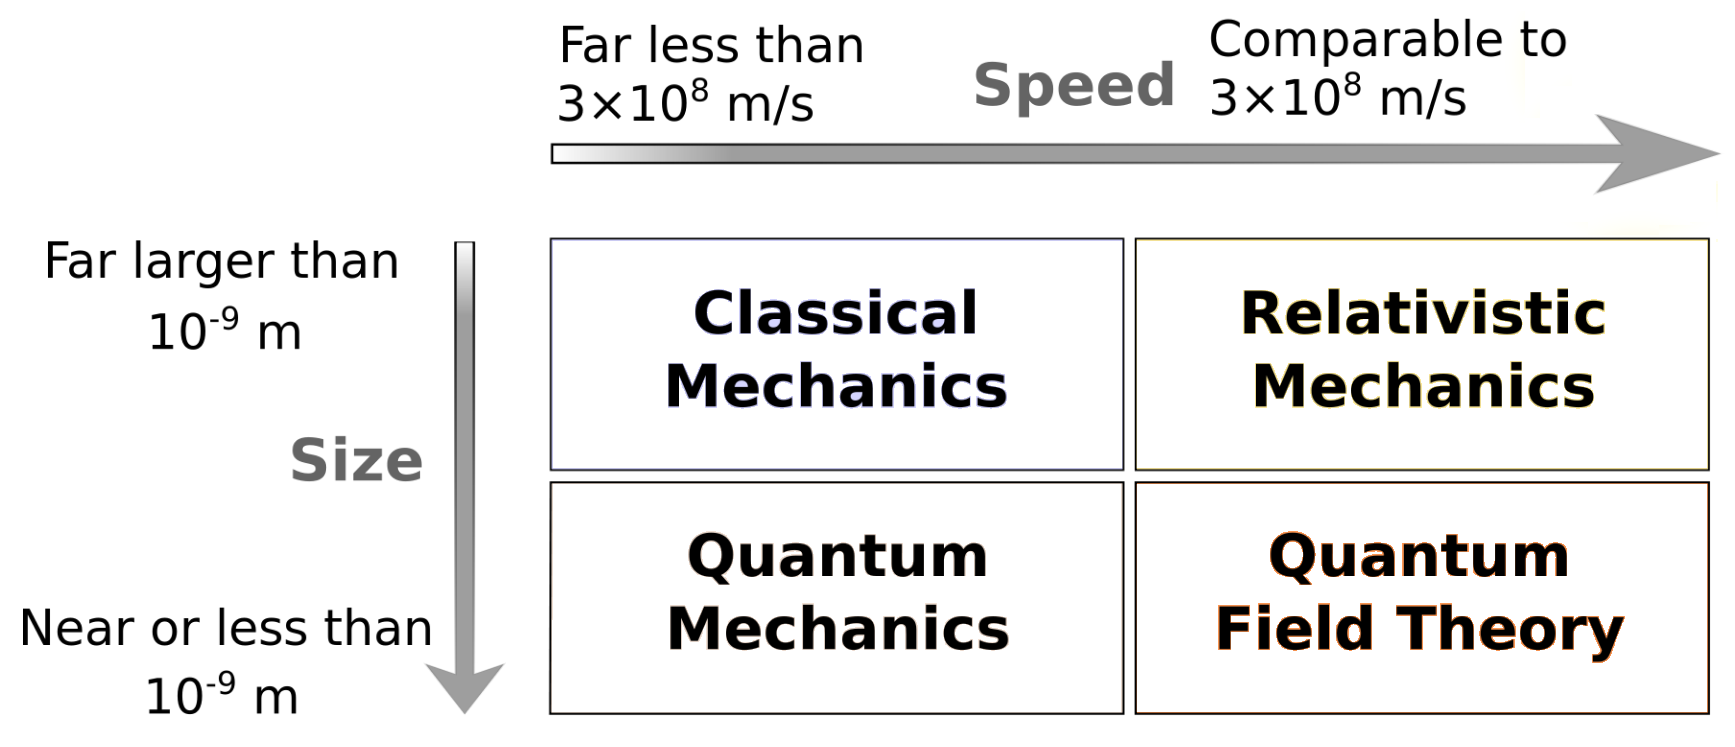
\includegraphics[width=0.6\textwidth]{figures/ov}
\end{figure}

\section{Notation}
\label{sec:notation}
\paragraph{Units:}
\index{Natural units}
Since this book will cover many different fields of physics will vary slightly throughout. As a rule of thumb; In the non-relativistic limit ($v\ll c$) SI units will be employed whereas in the relativistic limit ($v\simeq c$) natural units ($\hbar=k_B=c=1$) will be utilized. 

\paragraph{Vectors:}
Apart from the statistics part, a three vector will be denoted by a vector arrow, eg. $\vec{x}$, whereas a four vector will most often have no specific notation, eg. $x=x^\mu\doteq (x^0,x^1,x^2,x^3)^T$. A four vector with index up, eg. $x^\mu$, is a contravariant vector whereas a four vector with index down, eg. $x_\mu$, is a covariant vector (a deeper explanation and definition is found in section \ref{sec:lor}).

\paragraph{Derivatives:}
The partial derivative is denoted by $\partial_\mu= \frac{\partial}{\partial x^\mu}$ and the (Minkowski space) d'Alembertian is $\square=\partial_\mu\partial^\mu=\partial_0^2-\vec{\nabla}^2$. The symbol $\breve{\partial}_\mu$ is defined by $f\breve{\partial}_\mu g=f\partial_\mu g-(d_\mu f)g$.

\paragraph{Metric:}$\eta^{(qft)}_{\mu\nu} \doteq diag(1,-1,-1,-1)$ will be used in quantum field theory\footnote{Such that $x\cdot x=x_{(0)}x^{(0)}-(x_{(1)}x^{(1)}+x_{(2)}x^{(2)}+x_{(3)}x^{(3)})$.} and $\eta^{(sr)}_{\mu\nu}\doteq diag(-1,1,1,1)$ will be used in special relativity\footnote{Such that $x\cdot x=-x_{(0)}x^{(0)}+(x_{(1)}x^{(1)}+x_{(2)}x^{(2)}+x_{(3)}x^{(3)})$.}. Under normal conditions it will be quite clear which metric is used, and so the superscripts will be suppressed. A generic metric, valid in spaces which differ from Minkowski (special relativity), is denoted by $g_{\mu\nu}$. Often $g_{\mu\nu}$ and $\eta_{\mu\nu}$ will be used interchangeably.

\paragraph{Dirac matrices:} 
\index{Dirac matrices} 
Dirac matrices, $\gamma^\mu$, satisfy

\begin{equation}
	\{\gamma^\mu,\gamma^\nu\}=\gamma^\mu\gamma^\nu+\gamma^\nu\gamma^\mu=2\eta^{\mu\nu}.
\end{equation} 
Therefore $(\gamma^{0})^2=I\doteq1$ and $(\gamma^i)=-I\doteq -1$. $\gamma^0$ is hermitian whereas $\gamma^i$ is anti-hermitian, i.e.

\begin{equation}
	(\gamma^0)^\dagger=\gamma^0, \quad (\gamma^i)^\dagger=-\gamma^i \rightleftarrows (\gamma^\mu)^\dagger=\gamma^0\gamma^\mu\gamma^0,
\end{equation} 
where $\dagger=*T$ in matrix notation. The Dirac matrices satisfy the contraction identities

\begin{equation}
	\begin{split}
		\gamma^\mu\gamma_\mu&=\eta_{\mu\nu}\gamma^\mu\gamma^\nu=\frac{1}{2}g_{\mu\nu}\{\gamma^\mu,\gamma^\nu\}=\eta_{\mu\nu}\eta^{\mu\nu}=4,\\
		\gamma^\mu\gamma^\nu\gamma_\mu&=-2\gamma^\nu,\\
		\gamma^\mu\gamma^\nu\gamma^\alpha\gamma_\mu&=4\eta^{\nu\alpha},\\
		\gamma^\mu\gamma^\nu\gamma^\alpha\gamma^\beta\gamma_\mu&=-2\gamma^\beta\gamma^\alpha\gamma^\nu,\\
	\end{split}
\end{equation} 
where Einstein summations is used (repeated indices are summed implicitly). The matrix $\gamma^5$ is defined as follows

\begin{equation}
	\gamma^5\equiv i\gamma^0\gamma^1\gamma^2\gamma^3,
\end{equation} 
where

\begin{equation}
	(\gamma^5)^2=I\doteq 1, \quad (\gamma^5)^\dagger=\gamma^5, \quad \{\gamma^5,\gamma^\mu\}=0.
\end{equation} 
The commutator of the Dirac matrices is defined as follows

\begin{equation}
	[\gamma^\mu,\gamma^\nu]=\gamma^\mu\gamma^\nu-\gamma^\nu\gamma^\mu\equiv -2i\sigma^{\mu\nu},
\end{equation} 
where $\sigma^{\mu\nu}$ is a rank 2 tensor. The Dirac matrices obey the following trace identities

\begin{equation}
	\begin{split}
		Tr(I)&=Tr(1)=4,\\
		Tr(\gamma^\mu)&=0,\\
		Tr(\gamma^5)&=0,\\
		Tr(\text{odd $\#$ of $\gamma$'s})&=0,\\
		Tr(\gamma^\mu\gamma^\nu)&=4\eta^{\mu\nu},\\
		Tr(\gamma^\mu\gamma^\nu\gamma^\alpha\gamma^\beta\dots)&=Tr(\dots\gamma^\beta\gamma^\alpha\gamma^\nu\gamma^\mu),\\
		Tr(\gamma^5\gamma^\mu\gamma^\nu)&=0,\\
		Tr(\gamma^\mu\gamma^\nu\gamma^\alpha\gamma^\beta)&=4(\eta^{\mu\nu}\eta^{\alpha\beta}-\eta^{\mu\alpha}\eta^{\nu\beta}+\eta^{\mu\beta}\eta^{\nu\alpha}),\\
		Tr(\gamma^5\gamma^\mu\gamma^\nu\gamma^\alpha\gamma^\beta)&=-4i\varepsilon^{\mu\nu\alpha\beta},\\
	\end{split}
\end{equation} 

where $\varepsilon^{\dots}$ is the Levi-Civita tensor which obeys

\begin{equation}
	\begin{split}
		\varepsilon^{0123}&=1\\
		\varepsilon^{0132}&=-1\\
		\varepsilon^{\mu\nu\alpha\beta}\varepsilon_{\mu\nu\alpha\beta}&=-24,\\
		\varepsilon^{\mu\nu\alpha\beta}\varepsilon_{\mu\nu\alpha\sigma}&=-6\delta^\beta_{\,\,\, \sigma},\\
		\varepsilon^{\mu\nu\alpha\beta}\varepsilon_{\mu\nu\rho\sigma}&=-2(\delta^\alpha_{\,\,\, \rho}\delta^\beta_{\,\,\, \sigma}-\delta^\alpha_{\,\,\, \sigma}\delta^\beta_{\,\,\, \rho}).\\
	\end{split}
\end{equation} 
The Dirac matrices can be represented by several, equivalent, matrix representations (there is an ambiguity in the definition from the Dirac equation). Two often used representations are the Weyl representation (also called the chiral representation) and the standard representation

\begin{equation}
	\begin{split}
		&\text{Weyl rep.:} \quad \gamma^0\doteq \begin{bmatrix}
			0 & 1 \\
			1 & 0 \\
		\end{bmatrix}, \quad \gamma^i\doteq\begin{bmatrix}
			0 & \sigma^i \\
			-\sigma^i & 0 \\
		\end{bmatrix}, \quad \gamma^5\doteq\begin{bmatrix}
			-1 & 0 \\
			0 & 1 \\
		\end{bmatrix},\\
		&\text{Std. rep.:} \quad \gamma^0\doteq \begin{bmatrix}
			1 & 0 \\
			0 & -1 \\
		\end{bmatrix}, \quad \gamma^i\doteq\begin{bmatrix}
			0 & \sigma^i \\
			-\sigma^i & 0 \\
		\end{bmatrix}, \quad \gamma^5\doteq\begin{bmatrix}
			0 & 1 \\
			1 & 0 \\
		\end{bmatrix}.\\
	\end{split}
\end{equation} 
The above matrices are in block diagonal form. The Dirac matrices are $4\times 4$ matrices, so each block is $2\times 2$. $\sigma^i$ are called the Pauli matrices and are defined viz

\begin{equation}
	\sigma^1\doteq \begin{bmatrix}
		0 & 1\\
		1 & 0 \\
	\end{bmatrix}, \quad \sigma^2\doteq \begin{bmatrix}
		0 & -i\\
		i & 0 \\
	\end{bmatrix}, \quad \sigma^3\doteq \begin{bmatrix}
		1 & 0\\
		0 & -1 \\
	\end{bmatrix}.
\end{equation} 
The Pauli matrices satisfy

\begin{equation}
	\sigma^i \sigma^j=\delta^{ij}+i\varepsilon^{ijk}\sigma^k.
\end{equation} 
In relation to the Pauli matrices two 4-vectors are defined

\begin{equation}
	\sigma^\mu\equiv (1,\sigma^i), \quad \bar{ \sigma}^\mu\equiv (1,-\sigma^i).
\end{equation} 

\paragraph{Slash and bar notation:}
Feynman slash-notation is defined by

\begin{equation}
	\slashed A \equiv A_\mu\gamma^\mu=\gamma^\mu A_\mu=\gamma_\mu A^\mu=A^\mu\gamma_\mu.
\end{equation} 
Often the partial derivative will appear in slashed notation, i.e. $\slashed \partial =\gamma^\mu\partial _\mu$. The barred notation is defined by

\begin{equation}
	\bar{A}=A^\dagger \gamma^0_{Weyl},
\end{equation} 
where it is clear that the $\gamma^0$ to be used is only the one from the Weyl representation. The function of this $\gamma^0$ is to swap the upper and lower components in a $2\times 1$ matrix and this is what is needed. The $\gamma^0$ from the standard representation does not do this. Note however that henceforth the subscript on the $\gamma^0$ will be omitted and it it understood that for barred quantities (other than $\bar{\sigma}$ which is poorly defined in this notation) the relevant $\gamma^0$ is the one from the Weyl representation.

\paragraph{Dirac Spinors:} The Dirac spinors are defined as follows

\begin{equation}
	\begin{split}
		&u^s(\vec{p})=\begin{bmatrix}
			\sqrt{p\cdot \sigma}\xi^s\\
			\sqrt{p\cdot \bar{\sigma}}\xi^s\\
		\end{bmatrix}, \quad \bar{u}^s(\vec{p})=\begin{bmatrix}
			\xi^{\dagger s}\sqrt{p\cdot \sigma} & \xi^{\dagger s}\sqrt{p\cdot \bar{\sigma}}
		\end{bmatrix}\gamma^0, \\
		&v^{s'}(\vec{k})=\begin{bmatrix}
			\sqrt{k\cdot \sigma} \eta^{s'}\\
			-\sqrt{k\cdot \bar{\sigma}}\eta^{s'}
		\end{bmatrix}, \quad \bar{v}^{s'}(\vec{k})=\begin{bmatrix}
			\eta^{\dagger s'}\sqrt{k\cdot \sigma} & -\eta^{\dagger s'}\sqrt{k\cdot \bar{\sigma}}
		\end{bmatrix}\gamma^0,
	\end{split}
\end{equation} 
where\footnote{The identity $\xi^{\dagger s'}\eta^{s}=\delta^{ss'}$ encourages the identification $\xi=\eta$, just as \citet{Peskin1995}[p. 65] has done.} $\xi^{\dagger s'}\xi^s=\delta^{ss'}$, $\eta^{\dagger s'}\eta^s=\delta^{ss'}$, $\xi^{\dagger s'}\eta^{s}=\delta^{ss'}$ and the $\sqrt{p\cdot \sigma}$-like expressions are to be understood as the square root of the positive eigenvalue of the matrix $p\cdot \sigma$. Hence, the $\sqrt{p\cdot \sigma}$-like expressions are numbers and can be moved around as such. The $\sqrt{p\cdot \sigma}$-like expressions obey

\begin{equation}
	\begin{split}
		&\sqrt{p\cdot \sigma}=\sqrt{p^0-\vec{\sigma}\cdot\vec{p}}=\sqrt{eigenvals(p^0I-\vec{\sigma}\cdot\vec{p})}\\
		&\qquad \,\,\,\, =\begin{bmatrix}
			\sqrt{p^0-|\vec{p}|} & 0 \\
			0 & \sqrt{p^0+|\vec{p}|}\\
		\end{bmatrix},\\
		&\sqrt{p\cdot \bar{\sigma}}=\sqrt{p^0+\vec{\sigma}\cdot\vec{p}}=\sqrt{eigenvals(p^0I+\vec{\sigma}\cdot\vec{p})}\\
		&\qquad \,\,\,\, =\begin{bmatrix}
			\sqrt{p^0+|\vec{p}|} & 0 \\
			0 & \sqrt{p^0-|\vec{p}|}\\
		\end{bmatrix}.
	\end{split}
\end{equation} 
Since there are several eigenvalues which one is taken depends on the vector ($\xi,\eta$) which is multiplied (see \citealt{Lancaster2014}[p. 329]). For the Dirac spinors
\begin{equation}
	\begin{split}
		&u^{\dagger s}(\vec{p})u^{s'}(\vec{k})=\begin{cases}
			2p^0\delta^{ss'} & \text{if}\quad p=k\\
			\xi^{\dagger s'}[\sqrt{p\cdot \sigma}\sqrt{k\cdot \sigma}+\sqrt{p\cdot \bar{\sigma}}\sqrt{k\cdot \bar{\sigma}}\,]\xi^{s'}& \text{if}\quad p\neq k\\  
		\end{cases},\\
		&v^{\dagger s}(\vec{p})v^{s'}(\vec{k})=\begin{cases}
			2p^0\delta^{ss'} & \text{if}\quad p=k\\
			\eta^{\dagger s'}[\sqrt{p\cdot \sigma}\sqrt{k\cdot \sigma}+\sqrt{p\cdot \bar{\sigma}}\sqrt{k\cdot \bar{\sigma}}\,]\eta^{ s'}& \text{if}\quad p\neq k\\  
		\end{cases},\\
		&\bar{u}^{s}(\vec{p})u^{s'}(\vec{k})=\begin{cases}
			2m\delta^{ss'} & \text{if}\quad p=k\\
			\xi^{\dagger s'}[\sqrt{p\cdot \sigma}\sqrt{k\cdot \bar{\sigma}}+\sqrt{p\cdot \bar{\sigma}}\sqrt{k\cdot \sigma} \,]\xi^{ s'}& \text{if}\quad p\neq k\\  
		\end{cases},\\
		&\bar{v}^{s}(\vec{p})v^{s'}(\vec{k})=\begin{cases}
			-2m\delta^{ss'} & \text{if}\quad p=k\\
			-\eta^{\dagger s'}[\sqrt{p\cdot \sigma}\sqrt{k\cdot \bar{\sigma}}+\sqrt{p\cdot \bar{\sigma}}\sqrt{k\cdot \sigma} \,]\eta^{s'} & \text{if}\quad p\neq k\\ 
		\end{cases},\\
		&\bar{u}^{s}(\vec{p})v^{s'}(\vec{k})=\begin{cases}
			0 & \text{if}\quad p=k\\
			\xi^{\dagger s}[\sqrt{p\cdot \bar{\sigma}}\sqrt{k\cdot \sigma}-\sqrt{p\cdot \sigma}\sqrt{k\cdot \bar{\sigma}} \,] \eta^{s'} & \text{if}\quad p\neq k\\  
		\end{cases},\\
		&\bar{v}^{s}(\vec{p})u^{s'}(\vec{k})=\begin{cases}
			0 & \text{if}\quad p=k\\
			\eta^{\dagger s}[\sqrt{p\cdot \sigma}\sqrt{k\cdot \bar{\sigma}}-\sqrt{p\cdot \bar{\sigma}}\sqrt{k\cdot \sigma} \,] \xi^{s'}  & \text{if}\quad p\neq k\\  
		\end{cases}.\\
	\end{split}
\end{equation} 
Spin sums

\begin{equation}
	\sum_{s=1,2}u^s(\vec{p})\bar{u}^s(\vec{p})=\slashed p+m, \quad \sum_{s=1,2}v^s(\vec{p})\bar{v}^s(\vec{p})=\slashed p-m.
\end{equation} 
The solutions to Diracs equation should also be solutions to Klein-Gordons equation. The solutions to Klein-Gordons equation are plane waves, so $\psi\propto e^{\pm ip\cdot x}$ for Diracs equation. The "$\propto$" covers over $u^s(\vec{p}), v^s(\vec{o})$ (either of them). Using solutions on this form in Diracs equation results in a reduced equation from which (see equation \eqref{orse})
\begin{equation}
	\begin{split}
		u^s(\vec{p})&=\frac{\slashed p}{m}u^s(\vec{p}),\\
		\bar{u}^s(\vec{p})&=\bar{u}^s(\vec{p})\frac{\slashed p}{m},\\
		v^s(\vec{p})&=-\frac{\slashed p}{m}v^s(\vec{p}),\\
		\bar{v}^s(\vec{p})&=-\bar{v}^s(\vec{p})\frac{\slashed p}{m},\\
	\end{split}
\end{equation} 
These expressions are formidable for reducing terms on the form $\bar{u}^s(\vec{p})\Gamma v^{s'}(\vec{k})$. The procedure is as follows

\begin{equation}
	\begin{split}
		\bar{u}^s(\vec{p})\Gamma v^{s'}(\vec{k})&=\frac{1}{2}[\bar{u}^s(\vec{p})\Gamma v^{s'}(\vec{k})+\bar{u}^s(\vec{p})\Gamma v^{s'}(\vec{k})]\\
		&=\frac{1}{2}[\bar{u}^s(\vec{p})\frac{\slashed p}{m}\Gamma v^{s'}(\vec{k})-\bar{u}^s(\vec{p})\Gamma \frac{\slashed k}{m} v^{s'}(\vec{k})]\\
		&=\dots.
	\end{split}
\end{equation} 
To proceed use the specific form of $\Gamma$ alongside commutator relations and so forth.

\paragraph{Fourier transform:}
\index{Fourier transform}
The four dimensional Fourier transform is defined by

\begin{equation}
	\begin{split}
		f(x)&=\int \frac{d^4k}{(2\pi)^4}e^{-ik\cdot x}\tilde{f}(k),\\
		\tilde{f}(k)&=\int d^4x e^{ik\cdot x}f(x),\\
	\end{split}
\end{equation} 
where $x,k$ are four vectors of position an momentum, respectively and $\int d^4x=\int dx^0dx^1dx^2dx^3$. Taking the qft metric, the three dimensional Fourier transforms are defined by

\begin{equation}
	\begin{split}
		f(\vec{x})&=\int \frac{d^3k}{(2\pi)^3}e^{+i\vec{k}\cdot \vec{x}}\tilde{f}(\vec{k}),\\
		\tilde{f}(\vec{k})&=\int d^3x e^{-i\vec{k}\cdot \vec{x}}f(\vec{x}).\\
	\end{split}
\end{equation} 
For arbitrary $n$, the $n$-dimensional Dirac delta function satisfies

\begin{equation}
	\begin{split}
		\int_{-\infty}^\infty e^{-i\omega (t-t')}d\omega &=2\pi\delta(t-t'),\\
		\int d^4x e^{i(k+p)\cdot x}&=\int dx^0 e^{-i[-(k^0+p^0)]x^0}\int d^3xe^{-i(\vec{k}+\vec{p})\cdot \vec{x}},\\
		&=(2\pi)\delta[-(k^0+p_0)](2\pi)^3\delta^{(3)}(\vec{k}+\vec{p}),\\
		&=(2\pi)^4\delta^{(4)}(k+p),\\
		\int d^nx e^{i(k+p)\cdot x}&=(2\pi)^{n}\delta^{(n)}(k+p).
	\end{split}
\end{equation} 

\paragraph{Random variables:}
\index{Random variable}
The fundamental building blocks for statistics are random variables (usually denoted by $X$ or $Y$). A random variable is a way to quantify the outcome of a generic experiment. In practice this means mapping the sample space to a line of real numbers. The random variables are manipulated by operators, the most common of which are the expectation operator, $\mathbb{E}$ and the variance operator, $Var$. The two operators obey the identities
\begin{equation}
	\begin{split}
		&\mathbb{E}[X+Y]=\mathbb{E}[X]+\mathbb{E}[Y],\\
		&\mathbb{E}[aX]=a\mathbb{E}[X],\\
		&Var[X]\equiv \mathbb{E}[(X-\mathbb{E}[X])^2]\\
		&\qquad\quad=\mathbb{E}[X^2]-(\mathbb{E}[X])^2,\\
		&Var[a+X]=Var[X],\\
		&Var[aX]=a^2Var[X],\\
		&Var[aX+bY]=a^2Var[X]+b^2Var[Y]+2abCov[X,Y],\\
		&Var[aX-bY]=a^2Var[X]+b^2Var[Y]-2abCov[X,Y],\\
	\end{split}
\end{equation}
where
\begin{equation}
	\begin{split}
		Cov[X,Y]&=\mathbb{E}[(X-\mathbb{E}[X])(Y-\mathbb{E}[Y])]\\
		&=\mathbb{E}[XY]-\mathbb{E}[X]\mathbb{E}[Y],
	\end{split}
\end{equation}
where
\begin{equation}
	\begin{split}
		&Cov[X,a]=0,\\
		&Cov[X,X]=Var[X],\\
		&Cov[X,Y]=Cov[Y,X],\\
		&Cov[aX,bY]=abCov[X,Y],\\
		&Cov[a+X,b+Y]=Cov[X,Y],\\
		&Cov[aX+bY,cW+dV]=acCov[X,W]+adCov[X,V]+bcCov[Y,W]+bdCov[Y,V].\\
	\end{split}
\end{equation}
If two observations are independent, then $\mathbb{E}[XY]=\mathbb{E}[X]\mathbb{E}[Y]$. In this case it follows that the covariance vanishes. \newline\newline
The random variables can be either discrete or continuous. The random variable is discrete if the outcomes are countable, and continuous otherwise. Both discrete and continuous random variables are described by a probability function (PMF or PDF) and a cumulative function (CMF or CDF).

\paragraph{Discrete Random Variables}
In the case that the random variable, $X$, is discrete, the PMF will equal the point probability
\begin{equation}
	f(x_i)=\mathbb{P}(X=x_i),
	\label{eq1}
\end{equation} 
where
\begin{equation}
	f(x_i)>0\wedge \sum_{i=1}^{n}f(x_i)=1.
	\label{eq2}
\end{equation}
The CMF is an equivalent representation of data which is defined as
\begin{equation}
	F(x)=\mathbb{P}(X\leq x)=\sum_{x_i\leq x}f(x_i),
\end{equation}
where $0\leq F(x)\leq 1$. In the discrete case the expectation value and variance are defined viz.
\begin{equation}
	\mathbb{E}[X]=\sum_{x_i\leq x}x_if(x_i)
	,\qquad 
	Var[X]=\sum_{x_i\leq x}(x_i-\mu)^2f(x_i).
\end{equation}

\paragraph{Continuous Random Variables}
In the case that the random variable, $X$, is continuous the point probability will vanish since now the integral of the PDF must be unity, i.e. 
\begin{equation}
	\int_{-\infty }^{\infty }dx f(x)=1.
\end{equation}
Since the function integrated over an infinite interval must be finite, the value in any given point must vanish. Hence, in this case the PDF does not provide a probability but a probability density instead. The probability is obtained by integrating the PDF
\begin{equation}
	\mathbb{P}(A\leq X\leq B)=\int_{A}^{B}dxf(x)=F(B)-F(A),
\end{equation} 
where $F$ is the CDF defined as
\begin{equation}
	F(x)\equiv \int_{-\infty}^{x}dx'f(x').
\end{equation} 
In the continuous case the expectation value and variance are defined viz.
\begin{equation}
	\mathbb{E}[X]=\int_{-\infty}^{\infty}dx xf(x), \qquad
	Var[X]=\int_{-\infty }^{\infty}dx\bigg(x-\int_{-\infty}^{\infty}dx' x'f(x')\bigg)^2f(x).
\end{equation}

	\part{Classical Mechanics}
		\chapter{Newtonian Mechanics}
Newtonian mechanics is the framework, derived by Isaac Newton in $1687$, the describes physics of point particles in the non-relativistic, macroscopic limit (i.e. the limit in which the effect of relativity and quantum mechanics can be neglected). The centerpiece of Newtonian mechanics is Newtons five laws and the laws, the principle of conserved quantities and the choice of reference frame.


\section{Newtons laws}
\index{Newtons laws}
Armed with the enormous empirical material which is condensed in the laws of Kepler and Galileo, Isaac Newton managed to discover his famous laws of motion alongside the law of gravitational interaction. Newtons five laws of motion can be stated as follows~\citep{hjort}
\begin{enumerate}
	\item \emph{The law of inertia:} A body which is not acted upon by any force will either be at rest or in a state of uniform,  linear motion. This law is manifested in the definition of linear momentum. The linear momentum of an object is defined as the mass of the object, $m$, times the velocity of the object, $\vec{v}$, i.e.
	\begin{equation}
		\vec{p}=m\vec{v}=m\dot{\vec{x}},
	\end{equation} 
	where the dot indicates the time derivative of the position vector. From the definition of linear momentum, the law of inertia can be stated as follows
	\begin{equation}
		\text{No external force} \Rightarrow \vec{p}= \text{constant vector}.
	\end{equation} 
	In this way the law of inertia coincides with the law of conservation of linear momentum for an isolated particle. 
	
	\item \emph{The law of acceleration:} The mass, $m$, of a body, times its acceleration, $\vec{a}$, equals the force, $\vec{F}$, on the body, i.e. 
	\begin{equation}
		\vec{F}=m\vec{a}=m\ddot{\vec{x}},
	\end{equation} 
	where the dots denote the second time-derivative of the position vector. From the definition of linear momentum, the law of acceleration can be written as follows
	\begin{equation}
		\vec{F}=\frac{d\vec{p}}{dt}.
	\end{equation} 
	
	\item \emph{The law of action and reaction:} If body A acts on body B with a force, then body B will act on body A with an equal but oppositely directed force.
	
	\item \emph{The postulate of absolute time:} Absolute, true, and mathematical time, of itself, and from its own nature, flows equally without relation to anything external, and by another name is called duration.
	
	\item \emph{The postulate of absolute space:} Absolute space, in its own nature, without relation to anything external, remains always similar and immovable.
\end{enumerate} 
The five laws are, in the form stated above, only valid in what is called an inertial reference frame. An inertial reference frame is defined as a reference frame in which Newtons first law (the law of inertia) holds true. That is to say an inertial reference frame is a reference frame in which if an object is not subject to a resulting force, it will remain at rest or move with a uniform velocity, i.e. it will not accelerate. A non-inertial reference frame is a reference frame in which Newtons first law does not hold. Examples of non-inertial reference frames are eg. rotating reference frames or accelerating reference frames. The reader may be familiar with riding a marry-go-round or accelerating in a car. In both cases the reader might recall being pushed outwards or back into th seat. In both cases, the body is required to either hold onto the marry-go-round or push back into the seat, in order to remain at rest in the car or the marry-go-round. Hence, both of these reference frame are not inertial.
\begin{example}
	An important example of a force is the gravitational force in the Newtonian limit. Newtonian gravity states that the gravitational force between two particles act to attract the two particles. The force is given by
	\begin{equation}
		\vec{F}_g=-\frac{G_Nm_1m_2}{r^2}\hat{r}=m_1\vec{g},
	\end{equation} 
	where $G_N=6.67\cdot 10^{-11}\frac{Nm^2}{kg^2}$ is Newtons gravitational constant, $m_i$ are the masses of the two particles and $r$ is the radial vector connecting the two particles. The minus sign indicated the force is attractive.
\end{example}
\begin{example}
	\emph{Determine and solve the EOM for a simple pendulum.}\newline
	
	The simple pendulum is a mass hanging from a massless string, free to swing (see figure \ref{fig:pen}).
	\begin{figure}[H]
		\captionsetup{width=1\textwidth}
		\centering
		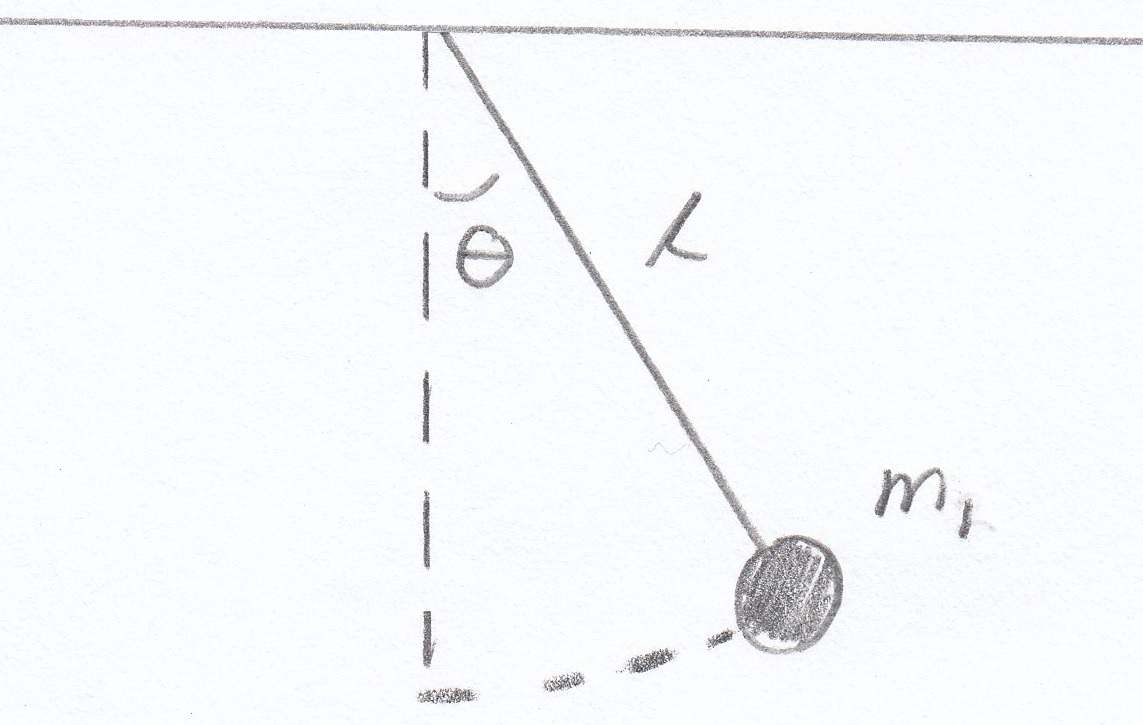
\includegraphics[width=0.3\textwidth]{figures/pen}
		\caption{The simple pendulum.}
		\label{fig:pen}
	\end{figure}
	From Newtons second law
	\begin{equation}
		\vec{F}_{res}=m_1\vec{a}
		=\vec{F}_g+\vec{F}_s,
	\end{equation} 
	where $\vec{F}_s$ is the force from the string onto the mass, $m_1$. $m_1$ does not move in the radial direction, so $\vec{F}_s$ must cancel the part of $\vec{F}_g$ in the radial direction,  i.e.
	\begin{equation}
		|\vec{F}_s|=-|\vec{F}_g|cos(\theta).
	\end{equation} 
	Therefore
	\begin{equation}
		m_1|\vec{a}|=-|\vec{F}_g|sin(\theta).
	\end{equation} 
	Now, $\vec{a}$ is the linear acceleration, in terms of the angular acceleration; $|\vec{a}|=\ddot{\theta}l$. Taking the small angle limit ($sin(\theta)\simeq \theta$), and using that $|\vec{F}_g|=m_1g$
	\begin{equation}
		\ddot{\theta}+\frac{g}{l}\theta\simeq 0\Rightarrow \theta\simeq \theta_0cos\bigg(\sqrt{\frac{g}{l}t}\bigg).
	\end{equation} 
	
\end{example}

\section{Non-inertial reference frames}
\index{Non-inertial reference frames}
When considering non-inertial reference frames it is desired to relate the force in a non-inertial reference frame to the forces in an inertial reference frame. Hence, the procedure of interest is how to transform Newtons second law from an inertial reference frame to a non-inertial reference frame. For this reason, a particle is considered from two different coordinate systems. One coordinate system, I, is an inertial reference frame that describes the location of the particle in terms of the position vector, $\vec{x}$. The non-inertial reference frame, I', performs a translating and rotating motion with respect to I. The distance from Origo in I to Origo in I' is defined by the vector $\vec{x}_0$, while the distance from Origo in I' to the particle is denoted by the vector $\vec{x'}$ (see figure \ref{fig:ref}).
\begin{figure}[h]
	\captionsetup{width=1\textwidth}
	\centering
	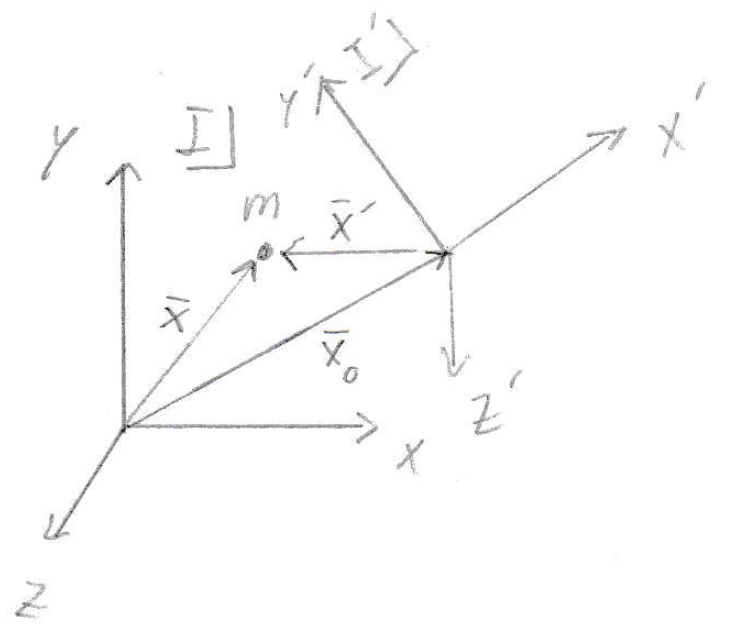
\includegraphics[width=0.5\textwidth]{figures/ref}
	\caption{The definition of the inertial an non-inertial reference frames, I,I', respectively.}
	\label{fig:ref}
\end{figure}
The two coordinate system could for example be the heliocentric reference frame as the inertial reference frame and the geocentric reference frame as the non-inertial reference frame\footnote{Depending on which approximations are made. Often the geocentric reference frame is taken to be an inertial reference frame. This is a valid approximation as long as the physical experiment under consideration does not span a significant portion of the Earth, i.e. as long as the experiment is confined to a smaller region of the Earth.}. From the definitions made in figure \ref{fig:ref} the position vector, $\vec{x}$, can be expressed in terms of $\vec{x}_0$ and $\vec{x'}$ viz
\begin{equation}
	\vec{x}=\vec{x}_0+\vec{x'}.
	\label{x1}
\end{equation} 
Equation \eqref{x1} can be used to relate the acceleration on $m_1$ as seen from I, I' by differentiating it twice with respect to time
\begin{equation}
	\begin{split}
		\ddot{\vec{x}}=\ddot{\vec{x}}_0+\ddot{\vec{x'}}+\vec{\omega}\times (\vec{\omega}\times \vec{x'})+2(\vec{\omega}\times \dot{\vec{x'}})+\dot{\vec{\omega}}\times \vec{x'}.
	\end{split}
	\label{x2}
\end{equation} 
By multiplying with the mass of the particle, and isolating $\vec{F}_{res,I'}=m\ddot{\vec{x'}}$ from equation \eqref{x2}
\begin{equation}
	\begin{split}
		\vec{F}_{res,I'}&=m\ddot{\vec{x'}}\\
		&=m[\ddot{\vec{x}}-\ddot{\vec{x}}_0-\vec{\omega}\times (\vec{\omega}\times \vec{x'})-2(\vec{\omega}\times \dot{\vec{x'}})-\dot{\vec{\omega}}\times \vec{x'}],\\
	\end{split}
	\label{x3}
\end{equation} 
where $\omega$ is the angular velocity of a given rotation around the axis going through the origin in I'. From equation \eqref{x3} it is clear that the resulting force in the reference frame of I' is equal to the resulting force in I subtracted some terms. These subtracted terms are what is called fictitious forces. Fictitious" because the forces are not real in the sense that they appear in an inertial reference frame. The fictitious forces represent the movement of the non-inertial reference frame, and as such they do not originate from any other body (as inertial forces do). The fictitious forces are defined as follows
\begin{equation}
	\begin{split}
		&\text{Origins; linear acceleration of I', wrt. I:}\qquad \ddot{\vec{x}}_0,\\
		&\text{Centrifugal acceleration:}\quad\qquad\quad\qquad\qquad\,\,\,\, \vec{\omega}\times (\vec{\omega}\times \vec{x'}),\\
		&\text{Coriolis acceleration: }\qquad\quad\quad\qquad\quad\qquad\,\,\,\, 2(\vec{\omega}\times \dot{\vec{x'}}),\\
		&\text{Azimuthal acceleration: }\qquad\quad\quad\qquad\qquad\,\,\,\, \dot{\vec{\omega}}\times \vec{x'}.\\
	\end{split}
\end{equation} 
The linear acceleration term is the one experience when sitting inside an accelerating car. The centrifugal term is one which is experience on a marry-go-round. The Coriolis term is more obscure. It is a force experience by particles which move in a rotating reference frame. For example, one would experience the Coriolis force if one walked around on a rotating marry-go-round. If one walked towards the center of a marry-go-round one would experience the Coriolis force pushing from the side. The azimuthal term, also called the Euler term, is also an obscure term. It is experience if the angular velocity of the rotating reference frame is changed. For example it would be experienced if the marry-go-round's rotational velocity accelerated or decelerated. If walking towards the center of a marry-go-round that is accelerating in rotational velocity, the azimuthal force would act to the opposite side as that of the Coriolis force. From the above definitions, the resulting force in a non-inertial reference frame can be written viz
\begin{equation}
	\vec{F}_{res,I'}=\vec{F}_{res,I}+\vec{F}_{trans}+\vec{F}_{centr}+\vec{F}_{cor}+\vec{F}_{azi},
\end{equation} 
where the fictitious forces are defined to absorb the minus signs.

\section{Center of mass}
Consider a system of point particles observed from some inertial reference frame, I. The particles might be mutually interacting (eg. via the gravitational interaction or the electromagnetic interaction) such that they form a rigid body. A rigid body is defined as a body consisting of many particles which do not change position during movement of the rigid body. The center of mass, with respect to origin in the inertial coordinate system, of both a system of particles and a rigid body is found by summing the positions of the individual particles weighted with their individual masses and divided by the total mass,  i.e.
\begin{equation}
	\vec{x}_{CM}=\frac{1}{m_{tot}}\sum_{i}m_i\vec{x}_i,
	\label{y1}
\end{equation} 
where $m_{tot}=\sum_i m_i$. Differentiating equation \eqref{y1} with respect to time, and taking $m_{tot}$ to the left hand side, reveals
\begin{equation}
	\begin{split}
		m_{tot}\vec{v}_{CM}=\sum_im_i\vec{v}_i=\sum_i\vec{p}_i=\vec{p}.
	\end{split}
	\label{y2}
\end{equation} 
Equation \eqref{y2} informs that the total, linear momentum of a system of particles, i.e. $\vec{p}$, is the sum of the linear momenta of all the constituent particles. Differentiating equation \eqref{y2} once more with respect to time
\begin{equation}
	\begin{split}
		\vec{F}_{res}&=\frac{d \vec{p}}{dt}=\sum_i \frac{d \vec{p}_i}{dt}=\sum_i m_i\ddot{\vec{x}}_i.\\
	\end{split}
	\label{y3}
\end{equation} 
The resulting force can be divided into two categories; the external forces and the internal forces. The external forces is forces that originate from bodies outside the system of particles whereas internal forces are forces that originate between constituents of the system of particles. According to Newtons third law (the law of action and reaction); the force from any particle onto another results in an equal force with opposite direction the other way around. Hence, denoting the force between particles $i,j$ as $\vec{F}_{ij}$
\begin{equation}
	\vec{F}_{ij}=-\vec{F}_{ji}.
	\label{y4}
\end{equation} 
Using equation \eqref{y4} in equation \eqref{y3} it is clear that the contribution to the resulting force from the internal forces vanish, and so
\begin{equation}
	\vec{F}_{res}=\sum_i\vec{F}_{ext,i}.
	\label{y5}
\end{equation} 
\paragraph{Center of mass theorem:}\index{Center of mass theorem} \emph{Hence, the entire mass of a system of particles, rigid or not, behaves as if the entire mass were concentrated in the center of mass and all external forces act in this point (from equation \eqref{y5}).} 
\paragraph{Conservation of linear momentum:} \index{Conservation of linear momentum} \emph{If no external forces act on a system of particles the total momentum, $\vec{p}$, of the system is a constant vector (from equation \eqref{y5}, \eqref{y3}).} \newline


\section{Energy}
Consider a particle, observed from an inertial reference frame, moving under the influence of a generic force, $\vec{F}$, which is taken to be a function of any relevant variables. When the particle is moved, by the force, from point a to point b, the force performs an amount of work, $W_{AB}$, on the particle, given by
\begin{equation}
	W_{ab}=\int_{a}^{b}\vec{F}\cdot d\vec{x}=\int\vec{F}\cdot\hat{n} d^3x,
	\label{w1}
\end{equation} 
where $\hat{n}$ is the unit tangent vector along the path of integration, i.e. the path along which which the particle is moving. Using Newtons second law equation \eqref{w1} can be written as follows
\begin{equation}
	W_{ab}=\int_a^bm\frac{d\vec{v}}{dt}\cdot d\vec{x}=\int_{a}^{b}m\vec{v}\cdot d\vec{v}=\frac{1}{2}mv_b^2-\frac{1}{2}mv_a^2.
	\label{w2}
\end{equation} 
The quantity $T=\frac{1}{2}mv^2$ is defined as the kinetic energy of the particle. From equation \eqref{w2} it is clear that the work done by all force acting on a particle equals the increase in kinetic energy of the particle,  i.e.
\begin{equation}
	W=\int\vec{F}\cdot d\vec{x}=\Delta T\Rightarrow dT=\vec{F}\cdot d\vec{x}\Rightarrow \frac{dT}{dt}=\vec{F}\cdot \vec{v}.
	\label{w3}
\end{equation} 
$\vec{F}\cdot \vec{v}$ is defined as the power done by the force $\vec{F}$. Related to the work integral is the definition of a conservative force and a conservative force field. 
\paragraph{Conservative force fields:}\index{Conservative force fields} \emph{A force field is called conservative if the work integral, $W_{ab}=\int_{a}^{b}\vec{F}\cdot d\vec{x}$, is independent on the path of integration, and depends only on the initial and final points.}

\paragraph{Central force fields:} \index{Central force fields} \emph{A central force field is a field where the force on the particle is always directed towards (or away from) a point, fixed in an inertial reference frame. This point is called the force center. All central force fields are conservative force fields and as such central force fields are a subgroup of conservative force fields.}\newline

A particle in a conservative force field has associated to it a potential energy, $V=V(\vec{x})$. The potential energy is defined with respect to some reference point and the notion of the "total potential energy" is senseless. Taking $U(P)=0$, the potential energy of a particle at point $a$ (in a conservative force field), is given by 
\begin{equation}
	V(\vec{a})=-\int_{P}^{a}\vec{F}\cdot d\vec{x}=-W_{ab}\Rightarrow \vec{F}=-\vec{\nabla}V(\vec{x}),
	\label{w4}
\end{equation}  
where $\vec{\nabla}=\begin{bmatrix}
	\partial_x & \partial_y & \partial _z\\
\end{bmatrix}^T$ is the gradient operator\footnote{A mathematical operator. Not to be confused with a quantum mechanical operator}. From equation \eqref{w4} it is clear that the potential energy is equal to minus the work done in moving a particle between two points. So, one can think of the potential energy as a means to store work. Consider now two arbitrary points in a conservative force field ($a,b$). For these points
\begin{equation}
	\int_P^a\vec{F}\cdot d\vec{x}=-V(a), \quad \int_P^b\vec{F}\cdot d\vec{x}=-V(b).
	\label{w5}
\end{equation} 
From equation \eqref{w5}
\begin{equation}
	\int_{a}^{b}\vec{F}\cdot d\vec{x}=\int_a^P\vec{F}\cdot d\vec{x}+\int_P^b\vec{F}\cdot d\vec{x}=V(a)-V(b).
	\label{w6}
\end{equation} 
Comparing equation \eqref{w6} to equation \eqref{w2}
\begin{equation}
	\frac{1}{2}mv_b^2-\frac{1}{2}mv_a^2=V(a)-V(b)\Rightarrow \frac{1}{2}mv_b^2+V(b)=\frac{1}{2}mv_a^2+V(a).
	\label{w8}
\end{equation}  
From equation \eqref{w8} it is clear that the sum of the kinetic and potential energy does not change as as the particle is moved, by a force, through a conservative force field. The sum of the kinetic and potential energy is defined as the mechanical energy, $E_{mek}$, so
\begin{equation}
	\text{In a conservative force field:}\quad E_{mek}=T+V=const.
\end{equation} 
\begin{example}
	\emph{A professional skier is skiing downhill  along the slope shown in figure \ref{fig:ski}. 
		\begin{figure}[H]
			\captionsetup{width=1\textwidth}
			\centering
			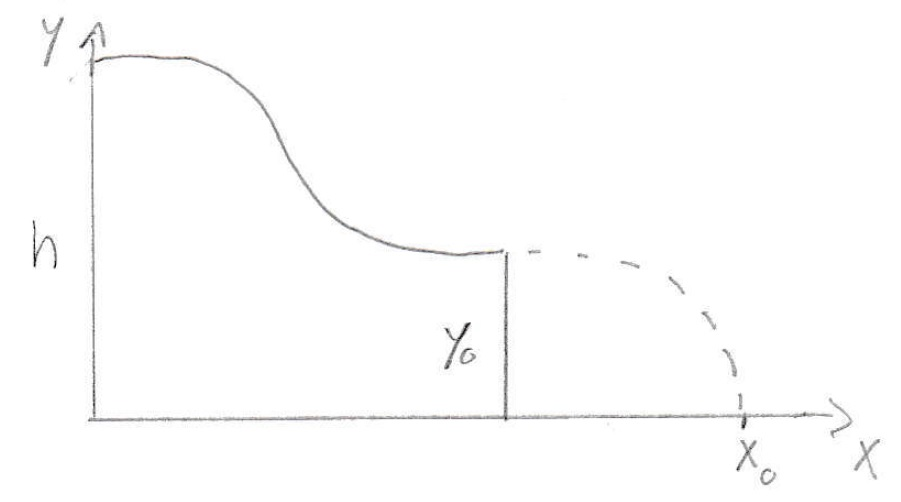
\includegraphics[width=0.3\textwidth]{figures/ski}
			\caption{The scenario of the ski-jumper.}
			\label{fig:ski}
		\end{figure}	
		The skier begins at $h=10m$ with $v=0\frac{m}{s}$. Assuming that there is no friction between the skies and the snow the skier arrives at the horizontal trampoline  with height $y_0$. Jumping out the skier lands at a distance $x_0$ from the horizontal trampoline.}
	
	\begin{enumerate}
		\item \emph{Determine the value of the trampoline hight, $y_0$, which maximizes $x_0$.}
		
		Since the skier is at rest when initiating the descend, from conservation of mechanical energy (no friction forces)
		\begin{equation}
			E_{mek}=mgh=\frac{1}{2}mv_0^2+mgy_0\Rightarrow v_0=\sqrt{2g(h-y_0)}.
		\end{equation} 
		Next use that the skier exits the jump at a horizontal direction. Subsequent to exiting the jump, the only force the skier is subject to is gravity. Since the gravitational acceleration is constant close to the Earth, the skier will take a time, $t_0$, before landing, given by
		\begin{equation}
			y_0=\frac{1}{2}gt_0^2\Rightarrow t_0=\sqrt{\frac{2y_0}{g}}.
		\end{equation} 
		During this time, the horizontal distance traversed is given by
		\begin{equation}
			x_0=v_0t_0\Rightarrow x_0=\sqrt{2g(h-y_0)}\sqrt{\frac{2y_0}{g}}=2\sqrt{hy_0-y_0^2}.
		\end{equation} 
		To maximize $x_0(y_0)$, isolate $y_0$ from $\frac{d x_0(y_0)}{dy_0}=0$ as follows
		\begin{equation}
			\frac{d x_0(y_0)}{dy_0}=\frac{h-2y_0}{\sqrt{hy_0-y_0^2}}=0 \Rightarrow y_0=\frac{h}{2}=5m.
		\end{equation} 
		$\frac{d^2x_0(y_0)}{dy_0^2}<0$ is indeed the case, so the point is a local maximum - Just as intended. This means $y_0=\frac{h}{2}=5m$ maximizes $x_0$.
		
		\item \emph{Determine the velocity of the skier when leaving the trampoline ($v_0$), and the distance in free air ($x_0$).}
		
		\begin{equation}
			\begin{split}
				&v_0=\sqrt{2g(h-\frac{h}{2})}=9.9\frac{m}{s},\\
				&x_0=\sqrt{2h^2-h^2}=10m.
			\end{split}
		\end{equation} 
	\end{enumerate}
\end{example}
\begin{example}
	\emph{An experienced mountaineer, which weights $m=80kg$, is climbing a near vertical wall. The mountaineer is secured against a possible fall by a climbing robe. One end of the robe is attached to the mountaineer while the other is secured by a pole in the rock below the mountaineer. The mountaineer climbs sufficiently high that he has used up the full length of the rope, $l_0$, which is still not stretched. This fill length of the rope is therefore identical to the difference in height between the mountaineer and the second pole below him. Assume negligible rope weight, and that the rope behaves as an ideal string with elastic constant $K=\frac{a}{l_0}$, with $a=40000N$.}
	
	\begin{enumerate}
		\item \emph{Determine the maximum tension of the rope if the mountaineer falls.}
		
		The physical scenario is modeled as shown in figure \ref{fig:moun}.
		\begin{figure}[H]
			\captionsetup{width=1\textwidth}
			\centering
			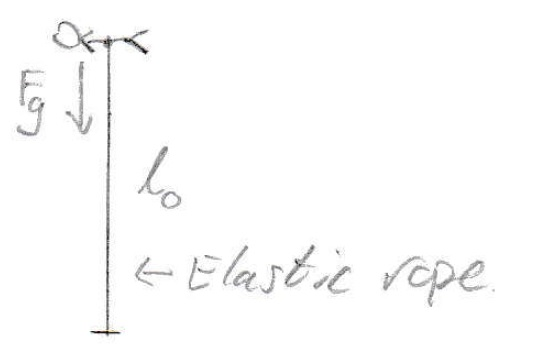
\includegraphics[width=0.3\textwidth]{figures/moun}
			\caption{The scenario of the mountaineer.}
			\label{fig:moun}
		\end{figure}
		Use that the maximum force from the rope is given by
		\begin{equation}
			F_{max}=kx_{max},
		\end{equation} 
		where $x_{max}$ is found by using the conservation of energy. The mountaineer initiates the fall with only potential energy. Subsequent to falling the mountaineer will stretch the rope and at some point, at which time the rope will eb stretched maximally, come to rest. When the rope is stretched maximally the tension of the rope will be at its highest, so 
		\begin{equation}
			\begin{split}
				E_{pot}&=mg(2l_0+x_{max})=\frac{1}{2}kx_{max}^2\\
				&\Rightarrow x_{max}=\frac{mg+\sqrt{(mg)^2+4Kmgl_0}}{k}\\
				&\Rightarrow F_{max}=mg+\sqrt{(mg)^2+4kmgl_0}\simeq 12 015 N.
			\end{split}
		\end{equation} 
	\end{enumerate}
\end{example}

\section{Angular momentum in classical mechanics}
Consider a particle of mass $m$ moving with a velocity $\vec{v}$ relative to some inertial reference frame I with origins in the point O. Relative to the point O, the angular momentum is defined as
\begin{equation}
	\vec{L}=\vec{x}\times \vec{p}=m\vec{x}\times \vec{v}=m rvsin(\theta),
	\label{ll1}
\end{equation} 
where $r=|\vec{x}|$ and $\theta$ is the angle between $\vec{v}$ and $\vec{x}$. The cross product multiplies the radius vector with the part of the velocity that is perpendicular to the radius vector. Differentiating equation \eqref{ll1} with respect to time reveals
\begin{equation}
	\frac{d\vec{L}}{dt}=\frac{d}{dt}(\vec{x}\times \vec{p})=\frac{d\vec{x}}{dt}\times \vec{p}+\vec{x}\times \frac{d\vec{p}}{dt}.
	\label{ll2}
\end{equation} 
Since $\frac{d\vec{x}}{dt}=\vec{v}\parallel \vec{p}$ the first term in equation \eqref{ll2} vanishes and so
\begin{equation}
	\frac{d\vec{L}}{dt}\vec{x}\times \frac{d\vec{p}}{dt}=\vec{x}\times\vec{F}.
\end{equation} 
The product $\vec{x}\times\vec{F}$ is defined as torque, $\vec{N}$, so
\begin{equation}
	\vec{N}\equiv \vec{x}\times\vec{F}=\frac{d\vec{L}}{dt}.
	\label{ll3}
\end{equation}  
\paragraph{The angular momentum theorem:}\index{Angular momentum theorem} \emph{The rate of change of the angular momentum of a particle around some point, O, equals the torque on the particle, with respect to O.}

\paragraph{Conservation of angular momentum:}\index{Conservation of angular momentum} \emph{If no torque acts on a particle, the angular momentum, around some point O, of that particle, with respect to the point O, is constant in time.}

\begin{example}
	A classic example of a system in which angular momentum is conserved is a central force field, eg. the gravitational field of a point particle. 
\end{example}
\begin{example}
	The angular momentum of a closed system, i.e. a system upon which no external forces act, is conserved. 
\end{example}

For a system of particles torque is given by
\begin{equation}
	\vec{N}_{res}=\sum_i\vec{N}_i=\sum_i\frac{d\vec{L}_i}{dt},
\end{equation} 
where $i$ runs over both external and internal forces. From Newtons third law $\vec{F}_{ij}=-\vec{F}_{ji}$, so for the internal torque
\begin{equation}
	\vec{N}_{ij}=\vec{x}_i\times \vec{F}_{ij}+\vec{x}_j\times \vec{F}_{ji}=(\vec{x}_i-\vec{x}_j)\times \vec{F}_{ij}=\vec{0}.
\end{equation} 
Hence, analogous to the case of Newtons second law for linear motion in which the resulting force was indifferent to the internal forces; the resulting torque is indifferent to the internal torques, so
\begin{equation}
	\vec{N}_{res}=\sum_{i}\vec{N}_{ext,i}.
\end{equation} 

\begin{example}
	\index{Planetary physics in Newtonian limit}
	\emph{Halley's comet is the most famous of all comets. It has a period of $76$ years and has been observed regularly since the battle of Hastings in $1066$. It has, in the point where it is closest to the Sun, a distance $r_0$ to the Sun, and a velocity $v_0$ relative to the heliocentric reference frame.}
	
	\begin{enumerate}
		\item \emph{Find a formal expression of the areal velocity of the comet, $\frac{dA}{dt}$, expressed in terms of $r_0$ and $v_0$.}
		
		Use that the cross product between two vectors denotes the area of the parallelogram they enclose (see figure \ref{fig:par}).
		\begin{figure}[h]
			\captionsetup{width=1\textwidth}
			\centering
			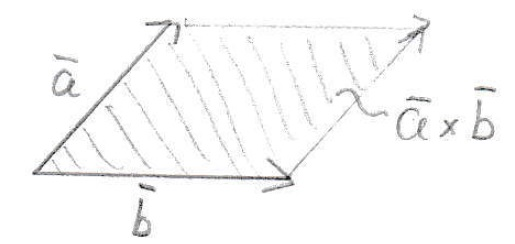
\includegraphics[width=0.3\textwidth]{figures/par}
			\caption{The parallelogram of the cross product.}
			\label{fig:par}
		\end{figure}
		The vectors relevant for the parallelogram in the physical scenario is $\vec{v}(t)$ and $\vec{r}(t+\Delta t)$ (see figure \ref{fig:par2}).
		\begin{figure}[h]
			\captionsetup{width=1\textwidth}
			\centering
			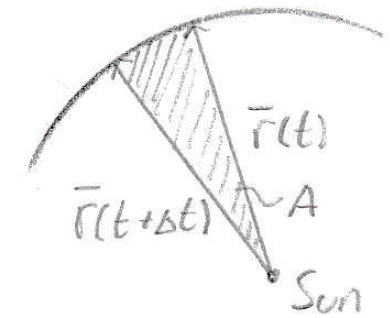
\includegraphics[width=0.3\textwidth]{figures/par2}
			\caption{The area under consideration.}
			\label{fig:par2}
		\end{figure}
		From figure \ref{fig:par2}
		\begin{equation}
			\Delta A=\frac{\vec{r}(t)\times \vec{r}(t+\Delta t)}{2}
			\label{A1}
		\end{equation} 
		Dividing equation \eqref{A1} by $\Delta t$ and taking the limit of $\Delta t\Rightarrow 0$
		\begin{equation}
			\begin{split}
				\frac{dA}{dt}&=\lim\limits_{\Delta t\Rightarrow 0}\bigg(\frac{\Delta A}{\Delta t}\bigg)=\lim\limits_{\Delta t\Rightarrow 0}\bigg(\frac{\vec{r}(t)\times \vec{r}(t+\Delta t)}{2\Delta t}\bigg)\\
				&=\lim\limits_{\Delta t\Rightarrow 0}\bigg(\frac{\vec{r}(t)\times (\vec{r'}(t)+\dot{\vec{r}}(t)\Delta t)}{2\Delta t}\bigg)\\
				&=\lim\limits_{\Delta t\Rightarrow 0}\bigg(\frac{\vec{r}(t)\times \dot{\vec{r}}(t)}{2}\frac{\Delta t}{\Delta t}\bigg)=\frac{\vec{r}(t)\times \vec{v}(t)}{2},\\
			\end{split}
		\end{equation} 
		where it has been used that $\vec{r}(t)\times \vec{r}(t)=\vec{0}$. Since the area velocity is constant the values of $v,r$ at the closest approach to the Sun can be used. At closest approach $\vec{v}_0\perp\vec{r}_0$, so
		\begin{equation}
			\frac{dA}{dt}=\frac{r_0v_0}{2}.
		\end{equation} 
		Alternatively, angular momentum can be used to obtain the same result. Consider figure \ref{fig:an}
		\begin{figure}[h]
			\captionsetup{width=1\textwidth}
			\centering
			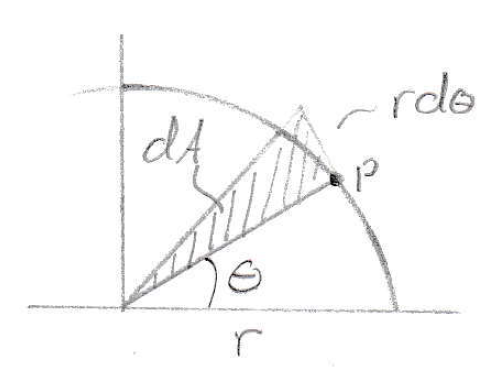
\includegraphics[width=0.3\textwidth]{figures/an}
			\caption{The orbit in polar coordinates.}
			\label{fig:an}
		\end{figure}
		From figure \ref{fig:an}
		\begin{equation}
			dA=\frac{1}{2}r^2d\theta\Rightarrow \frac{dA}{dt}=\frac{1}{2}r^2\frac{d\theta}{dt}.
			\label{r4}
		\end{equation} 
		To determine $\frac{d\theta}{dt}$ use conservation of angular momentum. The equation of motion for the comet is given by
		\begin{equation}
			m_C\ddot{\vec{r}}=-\frac{G_Nm_Cm_\odot}{|\vec{r}|^2}\frac{\vec{r}}{|\vec{r}|},
			\label{r1}
		\end{equation} 
		where $m_C$ is the mass of the comet and $m_\odot$ is the mass of the Sun. In polar coordinates
		\begin{equation}
			\ddot{\vec{r}}=\bigg(|\ddot{\vec{r}}|-|\vec{r}|\bigg(\frac{d\theta}{dt}\bigg)^2\bigg)\hat{e}_r+\frac{1}{|\vec{r}|}\frac{d}{dt}\bigg(|\vec{r}|^2\frac{d\theta}{dt}\bigg)\hat{e}_\theta.
			\label{r2}
		\end{equation} 
		Using equation \eqref{r2} in equation \eqref{r1} results in two equations; a radial and an angular
		\begin{equation}
			\begin{split}
				&\text{Radial:} \quad m_C\bigg(|\ddot{\vec{r}}|-|\vec{r}|\bigg(\frac{d\theta}{dt}\bigg)^2\bigg)\hat{e}_r=-\frac{G_Nm_Cm_\odot}{|\vec{r}|^2}\hat{e}_r,\\
				&\text{Angular:} \quad \frac{1}{|\vec{r}|}\frac{d}{dt}\bigg(|\vec{r}|^2\frac{d\theta}{dt}\bigg)\hat{e}_\theta=0.\\
			\end{split}
			\label{shi}
		\end{equation} 
		From the angular equation
		\begin{equation}
			\begin{split}
				\frac{d}{dt}\bigg(|\vec{r}|^2m_C\dot{\theta}\bigg)=0&\Rightarrow m_C|\vec{r}|^2\dot{\theta}=const\equiv L\\
				&\Rightarrow \dot{\theta}=\frac{L}{m_Cr^2},\\
			\end{split}
			\label{r3}
		\end{equation} 
		where $r=|\vec{r}|$. Using equation \eqref{r3} in equation \eqref{r4}
		\begin{equation}
			\frac{dA}{dt}=\frac{L}{2m_C}=\frac{m_C\vec{r}\times \vec{v}}{2m_C}=\frac{r_0v_0}{2}.
			\label{r15}
		\end{equation} 
		
		\item \emph{Find formal expressions of the angular momentum, $L$, and the total energy, $E_{mek}$, of the comet. From these two expressions obtain expressions for the eccentricity, $e$, the semi-major axis of the comets orbit, $a$, and the period, $T$, of the orbital motion. All expressions should be formulated in terms of $r_0$, $v_0$, $m_\odot$ and $G_N$.}
		
		Begin by considering the radial equation (equation \eqref{shi}). Substituting equation \eqref{r3} into the radial equation of equation \eqref{shi}
		\begin{equation}
			m_C\ddot{r}-r\frac{L^2}{m_Cr^4}=-\frac{G_Nm_Cm_\odot}{r^2}\Rightarrow \ddot{r}-\frac{L^2}{m_C^2r^3}=\frac{C}{m_Cr^2},
			\label{r5}
		\end{equation} 
		where $C\equiv-G_Nm_Cm_\odot$. Equation \eqref{r5} is a differential equation for $r(t)$, however, in relation to the orbit the quantity of interest is not $r(t)$, but rather $r(\theta)$. To introduce $r(\theta)$ into equation \eqref{r5}, use that
		\begin{equation}
			\begin{split}
				\ddot{r}&=\frac{d}{dt}\bigg(\frac{dr}{dt}\bigg)=\frac{d}{dt}\bigg(\frac{dr}{d\theta}\frac{d\theta}{dt}\bigg)=\frac{d}{dt}\bigg(\frac{dr}{d\theta}\frac{L}{m_Cr^2}\bigg)\\
				&=\frac{d}{d\theta}\bigg(\frac{dr}{d\theta}\frac{L}{m_Cr^2}\bigg)\frac{d\theta}{dt}=\frac{L^2}{m_C^2r^4}\frac{d^2r}{d\theta^2}+\frac{L^2}{m_C^2r^2}\bigg(-2r^{-3}\frac{dr}{d\theta}\bigg)\frac{dr}{d\theta}\\
				&=\frac{L^2}{m_C^2r^4}\bigg(\frac{d^2r}{d\theta^2}-\frac{2}{r}\bigg(\frac{dr}{d\theta}\bigg)^2\bigg).
			\end{split}
			\label{r6}
		\end{equation} 
		Next, introduce the variable $u=r^{-1}$, for which
		\begin{equation}
			\begin{split}
				\frac{d^2u}{d\theta^2}&=\frac{d}{d\theta}\bigg(\frac{du}{d\theta}\bigg)=\frac{d}{d\theta}\bigg(\frac{du}{dr}\frac{dr}{d\theta}\bigg)=\frac{d}{d\theta}\bigg(-r^{-2}\frac{dr}{d\theta}\bigg)\\
				&=\frac{d}{dr}\bigg(-r^{-2}\bigg)\bigg(\frac{dr}{d\theta}\bigg)^2+(-r^{-2})\frac{d^2r}{d\theta^2}\\
				&=\frac{2}{r^3}\bigg(\frac{dr}{d\theta}\bigg)^2-\frac{1}{r^2}\frac{d^2r}{d\theta^2}\\
				&=-\frac{1}{r^2}\bigg(\frac{d^2r}{d\theta^2}-\frac{2}{r}\bigg(\frac{dr}{d\theta}\bigg)^2\bigg).
			\end{split}
			\label{r7}
		\end{equation} 
		Comparing equation \eqref{r6} and \eqref{r7}
		\begin{equation}
			\ddot{r}=-\frac{L^2}{m_C^2r^2}\frac{d^2u}{d\theta^2}.
			\label{r8}
		\end{equation} 
		Using equation \eqref{r8} in equation \eqref{r5}, alongside the definition of $u=r^{-1}$
		\begin{equation}
			-\frac{L^2}{m_C^2}u^2\frac{d^2u}{d\theta^2}-\frac{L^2}{m_C^2}u^3=\frac{C}{m_C}u^2\Rightarrow \frac{d^u2}{d\theta^2}+u=-\frac{Cm_C}{L^2}.
			\label{r9}
		\end{equation} 
		Equation \eqref{r9} is an inhomogeneous, second order, linear, ordinary differential equation. The solution is a sum of \emph{one} solution to the inhomogeneous equation ($u_p$) and \emph{the} solution to the homogeneous equation ($u_h$). \emph{One} solution to the inhomogeneous equation is
		\begin{equation}
			u_p=-\frac{Cm_C}{L^2}.
		\end{equation} 
		The solution to the homogeneous equation is found via the conventional means (see \citealt{calculus})
		\begin{equation}
			u_h=Acos(\theta+\phi_0),
		\end{equation} 
		where $\phi_0$ is some phase. Hereby	
		\begin{equation}
			u=Bcos(\theta+\phi_0)-\frac{Cm_C}{L^2}.
			\label{r10}
		\end{equation} 
		By an appropriate placement of the coordinate system, $\phi_0=0$. To determine the integration-constant, $B$, initial conditions must be applied, or alternatively conservation laws. From conservation of energy
		\begin{equation}
			E_{mek}=\frac{1}{2}m_Cv^2+\frac{C}{r}=\frac{1}{2}m(\dot{r}^2+r^2\dot{\theta})+\frac{C}{r},
		\end{equation} 
		where polar coordinates have been used to express $v$. Using $\dot{\theta=\frac{L}{m_Cr^2}}$, from equation \eqref{r3}, the mechanical energy can be written as follows
		\begin{equation}
			E_{mek}=\frac{L^2}{2m_Cr^4}\bigg(\bigg(\frac{dr}{d\theta}\bigg)^2+r^2\bigg)+\frac{C}{r}.
			\label{r11}
		\end{equation} 
		Using equation \eqref{r10} in equation \eqref{r11}
		\begin{equation}
			\begin{split}
				\frac{dr}{d\theta}&=\frac{1}{B}\frac{sin(\theta)}{cos(\theta)^2}=Br^2sin(\theta)\\
				&\Rightarrow E_{mek}=\frac{L^2}{2m_Cr^4}\bigg(B^2r^4sin(\theta)^2+r^2\bigg)+\frac{C}{r}.\\
			\end{split}
			\label{r12}
		\end{equation} 		
		Using again equation \eqref{r10} in equation \eqref{r12}
		\begin{equation}
			E_{mek}=\frac{L^2B^2}{2m_C}-\frac{C^2m_C}{2L^2}\Rightarrow B=\sqrt{\bigg(E_{mek}+\frac{C^2m_C}{2L^2}\bigg)\frac{2m_C}{L^2}}.
			\label{r13}
		\end{equation} 
		Using equation \eqref{r13} in equation \eqref{r10}
		\begin{equation}
			\frac{1}{r}=\sqrt{\frac{2m_CE_{mek}}{L^2}+\frac{G_N^2m_\odot^2m_C^4}{L^4}}cos(\theta)+\frac{G_Nm_C^2m_\odot}{L^2}.
			\label{r14}
		\end{equation} 
		Equation \eqref{r14} can be written on the form of an ellipse equation,  i.e.
		\begin{equation}
			\frac{1}{r}=\frac{1}{p}(1+e\cdot cos(\theta)),
		\end{equation} 
		where
		\begin{equation}
			\begin{split}
				&p=\frac{L^2}{G_Nm_C^2m_\odot},\\
				&e=\sqrt{1+\frac{2E_{mek}L^2}{G_N^2m_C^3m_\odot^2}},
			\end{split}
		\end{equation} 
		where $e$ is the eccentricity of the orbit and $p$ is half the length of the chord perpendicular to the axis of the conic section and passing through the focus point. To get some results, use that from equation \eqref{r15}
		\begin{equation}
			\frac{dA}{dt}=\frac{L}{2m_c}\Rightarrow A=\frac{LT}{2m_C}=\pi ab=\pi a^2\sqrt{1-e^2},
			\label{r16}
		\end{equation} 
		where $a$ is the length of the semi-major axis, $b$ is the length of the semi-minor axis, $A=\pi ab$ is the area of an ellipse and $b=a\sqrt{1-e^2}$ is valid for an ellipse. Next use that
		\begin{equation}
			\begin{split}
				p&=a(1-e^2)=\frac{L^2}{G_Nm_c^2m_\odot}\\
				&\Rightarrow a=\frac{L^2}{G_Nm_C^2m_\odot}\frac{1}{1-e^2}=\frac{G_Nm_Cm_\odot}{2|E_{mek}|}.
			\end{split}
			\label{r17}
		\end{equation} 
		Using equation \eqref{r17} in equation \eqref{r16}
		\begin{equation}
			\begin{split}
				A&=\frac{LT}{2m_C}=\pi\bigg(\frac{G_Nm_Cm_\odot}{2|E_{mek}|}\bigg)^2\sqrt{1-e^2}\\
				&=\pi\bigg(\frac{G_Nm_Cm_\odot}{2|E_{mek}|}\bigg)^2\sqrt{\frac{2|E_{mek}|L^2}{G_N^2m_C^3m_\odot^2}}\\
				&=\pi G_NM_\odot L\sqrt{m_c}(2|E_{mek}|)^{-\frac{3}{2}}=\frac{\pi G_N m_\odot v_0r_0}{\big(v_0^2-\frac{2G_Nm_\odot}{r_0}\big)^{\frac{3}{2}}},
			\end{split}
		\end{equation} 
		where $L,E_{mek}$ has been inserted for the last equality. Using $E_{mek}$ in equation \eqref{r17}
		\begin{equation}
			a=\frac{G_N M_\odot m_C}{2|E_{mek}|}=\frac{1}{\frac{v_0^2}{G_Nm_\odot}-\frac{2}{r_0}}
		\end{equation} 
		Lastly, the period of the orbit:
		\begin{equation}
			T=\frac{2m_CA}{L}=\frac{2\pi G_N m_\odot}{\big(v_0^2-\frac{2G_Nm_\odot}{r_0}\big)^{\frac{3}{2}}}
		\end{equation} 
		
		\item \emph{Find numerical values for $e$ and $T$ by using $r_0=0.5870 AU$, $1AU= 1.496\cdot 10^9m$, $v_0=54.53\frac{km}{s}$, $G_N=6.76\cdot 10^{-11}\frac{Nm^2}{kg^2}$ and $m_\odot=1.989\cdot 10^30kg$.}
		
		By inserting the numbers:
		\begin{equation}
			\begin{split}
				&a=\frac{G_Nm_\odot}{2|\frac{1}{2}v_0^2-\frac{G_Nm_\odot}{r_0}|}\simeq 2.69\cdot 10^9 km\simeq 18 AU\\
				&e=\sqrt{1+\frac{v_0^4r_0^2-2G_Nm_\odot v_0^2r_0}{G_N^2m_\odot^2}}\simeq 0.967\\
				&T=\frac{2\pi a^2\sqrt{1-e^2}}{r_0v_0}\simeq 76.28\, years
			\end{split}
		\end{equation} 		
	\end{enumerate}
\end{example}

\begin{example}
	\index{Planetary physics in Newtonian limit}
	\emph{The Enterprise's last tour into darkness has been completed. After the last deep-space mission the spaceship has re-entered the Solar system. It is now on a circular orbit of radius $R_0$ around the Earth. The Enterprise has velocity $\vec{v}_0$ with respect to the reference frame with origin in the center of the Earth and the axis towards what seems to be the fixed stars in the night sky. Consider this reference frame to be inertial. Upon the sudden news that a new super villain is attacking the headquarters of the intergalactic confederation fleet, the Enterprise moves from a circular orbit of radius $R_0$ to another, elliptical orbit, with perigee, $P$, at a distance, $R$, from the center of the Earth. During this maneuverer the Enterprise expels the mass $m_1$ of fuel while acquiring the velocity $\vec{v}_1=\vec{v}_0+\Delta\vec{v}$ with $\Delta\vec{v}$ in the direction of the Earths center. When the Enterprise passes through the perigee, $P$, again, it ejects fuel of mass $m_2$ to acquire the escape velocity tangent to the elliptic orbit. 
		In all the cases considered above, assume, for simplicity, that the fuel is expelled instantaneously and that the modulus of its speed relative to the Enterprise,	after been expelled, is $v_r$. Lieutenant Commander Spock (you) acquires the following data from the command deck: $R=0.91R_0$ and $v_r=2\sqrt{\frac{G_NM_E}{R_0}}$. 
		James T. Kirk, the commander of the Enterprise, asks the Lieutenant Commander Spock (you):}
	
	\begin{enumerate}
		\item \emph{What is the ratio between the mass $m_1+m_2$ of fuel consumed and the total mass, $m_s$, of the Enterprise?}
		
		The physical scenario is shown in figure \ref{fig:ent}.		
		\begin{figure}[h]
			\captionsetup{width=1\textwidth}
			\centering
			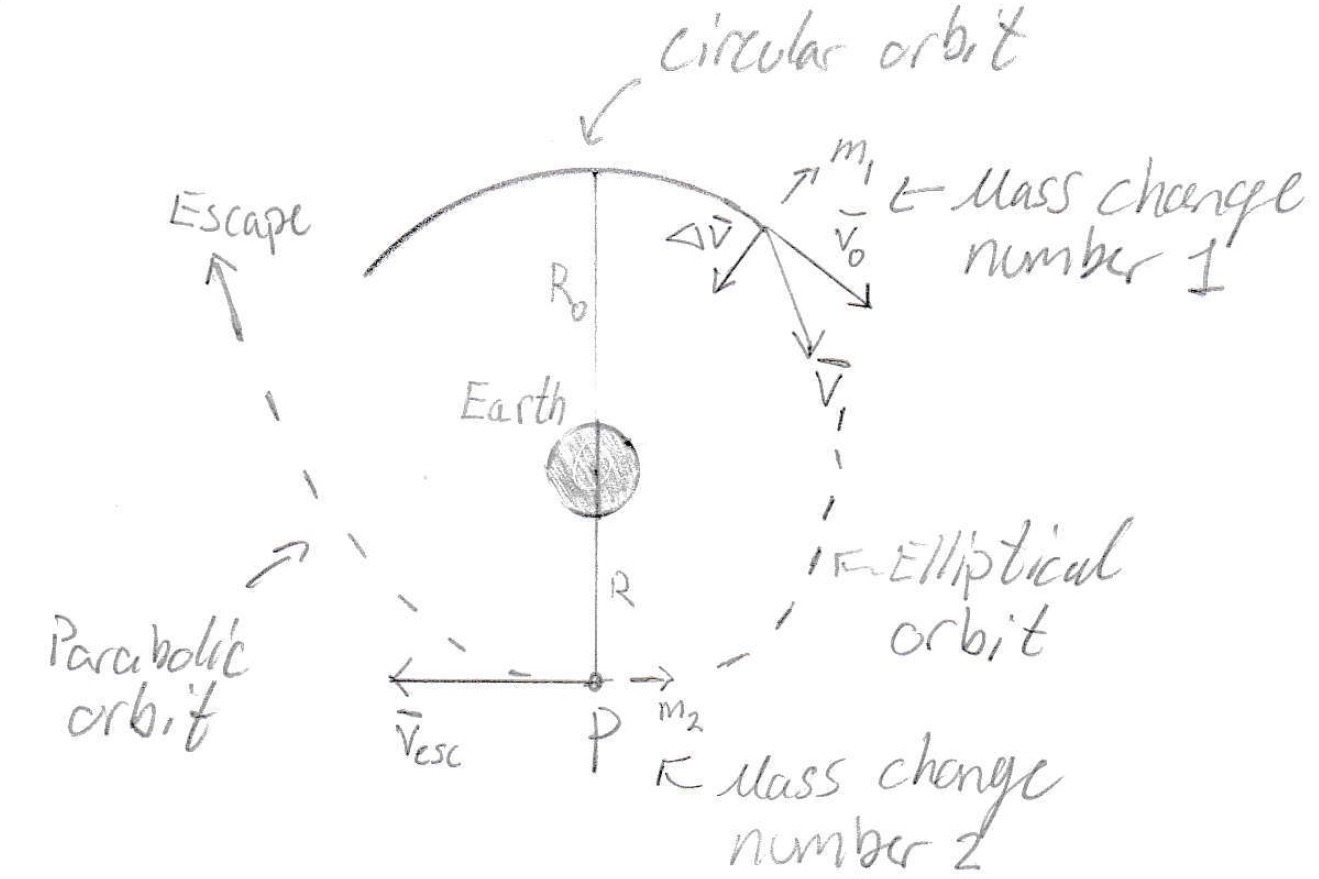
\includegraphics[width=0.8\textwidth]{figures/ent}
			\caption{The scenario of the Enterprise.}
			\label{fig:ent}
		\end{figure}
		The goal is to determine: $\text{Ratio 1}=\frac{m_1+m_2}{m_s}$. To do so, $m_1$ must be specified in terms of $m_2$ and $m_s$ must be specified in terms of $m_1,m_2$. The plan is to use conservation of linear and angular momentum to do so. Conservation across the first ejection of mass dictates:
		\begin{equation}
			\begin{split}
				m_s\vec{v}_0&=(m_s-m_1)(\vec{v}_0+\Delta\vec{v}_1)+m_1\vec{u}_1\\
				&=m_s\vec{v}_0+m_s\Delta\vec{v}_1+m_1(\vec{u}_1-\vec{v}_0-\Delta\vec{v}_1)\\
				&=m_s\vec{v}_0+m_s\Delta\vec{v}_1+m_1\vec{v}_r\\
				&\Rightarrow \Delta \vec{v}_1=-\frac{m_1}{m_s}\vec{v}_r\\
			\end{split}
		\end{equation} 
		where $\Delta \vec{v}_i$ denotes the velocity gained, $\vec{u}_i$ denotes the velocity of the fuel with respect to the (approximated) inertial reference frame of the Earth and $\vec{v}_r=\vec{u}-\vec{v}_0-\Delta\vec{v}_1$ is the relative velocity between the Enterprise and the fuel after it has been ejected. $\Delta \vec{v}_1\perp \vec{v}_0$, so $v_1^2=v_0^2+\Delta v_1^2+2\vec{v}_0\cdot \Delta \vec{v}_1=v_0^2+\Delta v_1^2=v_0^2+\big(\frac{m_1}{m_s}v_r\big)^2$. Hence, $v_1(v_0,m_1,m_s)$ has been determined. In order to determine the relation between $m_1$ and $m_s$, another (independent) equation for $v_1$ must be obtained. Such an equation comes from energy conservation between ejection of $m_1$ and $m_2$:
		\begin{equation}
			\begin{split}
				E_{mek}&= \frac{1}{2}(m_s-m_1)v_1^2-\frac{G_N(m_s-m_1)m_E}{R_0}\\
				&=\frac{1}{2}(m_s-m_1)v_p^2-\frac{G_N(m_s-m_1)m_E}{0.91R_0}\\
			\end{split}
			\label{l3}
		\end{equation} 
		To express the gravitational potential energy in terms of the circular, orbital velocity, $v_0$, use that for a circular orbit the eccentricity vanishes,  i.e.
		
		\begin{equation}
			\begin{split}
				e&=\sqrt{1+\frac{2E_{mek}L^2}{G_N^2m_s^3m_E^2}}=0\\
				&\Rightarrow \frac{2E_{mek}L^2}{G_N^2m_s^3m_E^2}=-1\\
				&\Rightarrow E_{mek}=\frac{G_N^2m_s^3m_E^2}{2L^2}=-\frac{G_N^2m_sm_E^2}{2(R_0v_0)^2}\\
			\end{split}
		\end{equation} 
		\normalsize
		where $L=v_0R_0$ for a circular orbit. From this the velocity of the circular orbit can be determined:
		\begin{equation}
			E_{mek}=\frac{1}{2}m_sv_0^2-\frac{G_Nm_sm_E}{R_0}=-\frac{G_N^2m_E^2m_s}{2R_0^2v_0^2}\Rightarrow v_0=\sqrt{\frac{G_Nm_E}{R_0}}
			\label{v_0}
		\end{equation} 
		Using equation \eqref{v_0} in equation \eqref{l3}
		\begin{equation}
			\begin{split}
				v_p^2&=v_1^2+2v_0^2\bigg(\frac{1}{0.91}-1\bigg)\\
				&=v_0^2+\frac{2m_1}{m_s}v_0^2+2v_0^2\bigg(\frac{1}{0.91}-1\bigg)\\
				&=v_0^2\bigg[\bigg(\frac{2m_1}{m_s}\bigg)^2+\frac{2}{0.91}-1\bigg].\\
			\end{split}
			\label{l5}
		\end{equation} 
		$v_p$ can be determined from conservation of angular momentum between ejection of $m_1$ and $m_2$. Just after $m_1$ is ejected
		\begin{equation}
			\vec{L}_1=(M-m_1)\vec{R}_0\times \vec{v}_1.
		\end{equation} 
		The cross product multiplies $R_0$ with the part of $\vec{v}_1$ perpendicular to $\vec{R}_0$, so
		\begin{equation}
			L_1=(M-m_1)R_0v_0.
			\label{l1}
		\end{equation} 
		Just before the Enterprise ejects the second mass, $m_2$, at perigee
		\begin{equation}
			L_2=(M-m_1)Rv_p=0.91R_0v_p.
			\label{l2}
		\end{equation} 
		Equating equation \eqref{l1} and \eqref{l2}
		\begin{equation}
			v_0=0.91v_p.
			\label{l4}
		\end{equation} 
		Using equation \eqref{l4} in equation \eqref{l5} reveals
		\begin{equation}
			m_s=\frac{2\cdot 0.91}{1-0.91}m_1\simeq 20.22 m_1.
			\label{l6}
		\end{equation} 
		With equation \eqref{l6} in the bag only a relation between $m_1$ and $m_2$ is needed to determine the desired ratio. such an expression is obtained from conservation of momentum across the second mass ejection
		\begin{equation}
			\begin{split}
				(m_s-m_1)\vec{v}_p&=(m_s-m_1-m_2)(\vec{v}_p+\Delta \vec{v}_2)+m_2\vec{u}_2\\
				&=(m_s-m_1)(\vec{v}_p+\Delta \vec{v}_2)+m_2(\vec{u}_2-\vec{v}_p-\Delta \vec{v}_2)\\
				&=(m_s-m_1)\vec{v}_{esc}+m_2\vec{v}_r.\\
			\end{split}
		\end{equation} 
		Since the mass is pushed directly backwards from the Enterprise this time
		\begin{equation}	
			(m_s-m_1)v_p=(m_s-m_1)v_{esc}-m_2v_r,
			\label{l7}	
		\end{equation} 
		where the direction has been extracted from $\vec{v}_r$. $v_{esc}$ can be specified in terms of $v_0$ by using that $v_{esc}$ is defined as the velocity which corresponds to $E_{mek}=0$,  i.e.
		\begin{equation}
			\begin{split}
				E_{mek}&=\frac{1}{2}(m_s-m_1-m_2)v_{esc}^2-\frac{G_N(m_s-m_1-m_2)m_E}{R}=0\\
				&\Rightarrow v_{esc}=\sqrt{\frac{2}{0.91}}v_0.
			\end{split}
			\label{l8}
		\end{equation} 
		Using equation \eqref{l8}, \eqref{v_0} and $v_r=2v_0$ in equation \eqref{l7}
		\begin{equation}
			m_s= m_1+\frac{2}{\sqrt{\frac{2}{0.91}}-\frac{1}{0.91}}m_2\simeq m_1+5.21m_2.
			\label{l9}
		\end{equation} 
		Equating equation \eqref{l6} and \eqref{l9}
		\begin{equation}
			m_2\simeq\frac{1}{2}\bigg(\frac{2\cdot 0.91}{1-0.91}-1\bigg)\bigg(\sqrt{\frac{2}{0.91}}-\frac{1}{0.91}\bigg) m_1\simeq 3.69 m_1.
		\end{equation} 
		Hereby, the ratio is given by
		\begin{equation}
			\text{Ratio 1}=\frac{m_1+m_2}{m_s}\simeq 0.23.
			\label{ratio1}
		\end{equation} 
		
		\item \emph{Compare the previous ratio with the ratio $\frac{m_3}{m_s}$, where $m_3$ is the fuel needed for the Enterprise to escape the Earths gravitational field directly from circular orbit of radius $R_0$. $m_3$ is assumed to be ejected tangentially to the circular orbit.}
		
		When escaping directly from circular orbit
		\begin{equation}
			v_{esc}=\sqrt{\frac{2G_Nm_E}{R_0}}=\sqrt{2}v_0.
		\end{equation} 
		Conservation of linear momentum across the ejection of $m_3$ dictates
		\begin{equation}
			\begin{split}
				m_s\vec{v}_0&=(m_s-m_3)(\vec{v}_0+\Delta \vec{v}_3)+m_3\vec{u}_3\\
				&=m_s(\vec{v}_0+\Delta \vec{v}_3)+m_3(\vec{u}_3-\vec{v}_0-\Delta \vec{v}_3)\\
				&=m_s\vec{v}_{esc}+m_3\vec{v}_r.\\
			\end{split}
		\end{equation} 
		Since the mass is ejected directly backwards from the Enterprise
		\begin{equation}
			\begin{split}
				m_sv_0&=m_sv_{esc}-m_3v_r\\
				&=m_s\sqrt{\frac{2}{0.91}}v_0-2m_3v_0\\
				&\Rightarrow m_s=\frac{2}{\sqrt{\frac{2}{0.91}}-1}m_3\simeq 4.15 m_3.
			\end{split}
		\end{equation} 
		So, the new ratio is given by
		\begin{equation}
			\text{Ratio 2}=\frac{m_3}{m_s}\simeq 0.24.
			\label{ratio2}
		\end{equation} 
		Comparing equation equation \eqref{ratio1} and \eqref{ratio2} reveals a small difference. Escaping directly from circular orbit seems to require more fuel than escaping via an elliptical orbit. The reason for this is that whilst in the elliptical orbit the Enterprise is accelerated by the gravitational field of the planet. This procedure is well known and often used in space-travel. the procedure of using the gravitational field of an object in space to accelerate a spacecraft is called a gravitational assist.
	\end{enumerate}
\end{example}

\section{Navier-Stokes Equation}
\index{Navier-Stokes equation}
An important application of Newtonian mechanics is to derive the fundamental equation of fluid dynamics; the Navier-Stokes equation. The Navier-Stokes equation is derived from Cauchy's equation which describes a generic fluid. Cauchy's equation can be derived from Newtons second law, $\vec{F}=m\vec{a}$, and is as such valid only in the non-relativistic limit- Just as Newtons second law. To derive Cauchy's equation the forces on a material particle, flowing along a stream in a fluid, is considered. The material particle is taken to be a small portion of the fluid which contains millions of molecules. Hence, the material particle is a small part of the fluid, but not at the quantum mechanics level (size $~$ molecule). Newtons second law for the material particle can be written as follows
\begin{equation}
	\vec{F}=m_p\frac{d\vec{v}_{p}}{dt},
\end{equation}   
where $\vec{v}_p$ is the velocity and $m_p$ is the mass - Both of the material particle. It is convenient to express the acceleration in terms of the velocity field ($v_f(x(t),y(t),z(t),t)$) of the fluid instead of the velocity of the material particle. In terms of the velocity field the derivative of the velocity of the particle is given by
\begin{equation}
	\begin{split}
		\frac{d\vec{v}_{p}}{dt}&=\frac{\partial \vec{v}_f}{\partial t}+\sum_{i=1}^{3}\frac{\partial \vec{v}_f}{\partial x_i}\frac{\partial x_i}{\partial t}\\
		&=\frac{\partial \vec{v}_f}{\partial t}+\vec{v}_f\cdot (\vec{\nabla}\cdot\vec{v}_f).
	\end{split}
	\label{N1}
\end{equation} 
The first term in equation \eqref{N1} accounts for the time-variation in the velocity field at a given point whereas the second term, called the advective acceleration, accounts for how the velocity field changes as a particle travels through the field (as seen from the perspective of the particle). Factorizing $\vec{v}_f$ in equation \eqref{N1} leads to the definition of the material derivative. The material derivative is a differential operator given by
\begin{equation}
	\frac{D}{Dt}\equiv \frac{\partial }{\partial t}+\vec{v}_f\cdot \vec{\nabla}.
\end{equation}  
By using the definition of the material derivative Newtons second law can be written in terms of the velocity field. Dividing through with the volume of the material particle and writing the force as a sum of surface forces ($\vec{f}_{s}$) and body forces ($\vec{f}_{b}$) results in
\begin{equation}
	\rho_p\frac{D\vec{v}_f}{Dt}=\vec{f}_{b}+\vec{f}_{s}.
	\label{N2}
\end{equation} 
Among body forces is gravity, electromagnetic forces and fictitious forces. Among surface forces is pressure forces and viscous forces. The surface forces can be specified in terms of the stress tensor. The stress tensor can always be separated into two parts; a pressure part and a shear stress-part viz
\begin{equation}
	\sigma_{ij}=-p\delta_{ij}+\tau_{ij}.
\end{equation}  
The surface forces are given in terms of the divergence of the stress tensor,  i.e.
\begin{equation}
	\begin{split}
		\vec{f}_s&=\vec{\nabla}\cdot \sigma\\
		&=-\vec{\nabla}p+\sum_{i,j}\partial_j \tau_{ij} \hat{e}_i\\
		&=-\begin{bmatrix}
			\frac{\partial p}{\partial x}\\
			\frac{\partial p}{\partial y}\\
			\frac{\partial p}{\partial z}\\
		\end{bmatrix}+\begin{bmatrix}
			\sum_{j=x,y,z} \frac{\partial \tau_{xj}}{\partial x_j}\\
			\sum_{j=x,y,z} \frac{\partial \tau_{yj}}{\partial x_j}\\
			\sum_{j=x,y,z} \frac{\partial \tau_{zj}}{\partial x_j}\\
		\end{bmatrix}.
	\end{split}
	\label{N3}
\end{equation} 
Using equation \eqref{N3} in equation \eqref{N2} results in Cauchy's equation
\begin{equation}
	\rho_p\frac{D\vec{v}_f}{Dt}=\vec{f}_{b}-\vec{\nabla}p+\sum_{i,j}\partial_j \tau_{ij} \hat{e}_i.
	\label{N4}
\end{equation} 
Cauchy's equation (equation \eqref{N4}) is valid for all non-relativistic fluids (gases and liquids). The Navier-Stokes equation is obtained from Cauchy's equation by approximating the fluid under consideration as isotropic, Newtonian and with a constant viscosity. Taking the fluid to be isotropic and Newtonian means that the different shear components of the stress tensor can be expressed in terms of velocity gradients since it is changes in the fluid velocity that creates stress in the fluid,  i.e.
\begin{equation}
	\begin{split}
		&\text{Newtonian:} \quad\, \sigma_{ij}=\eta\frac{d v_x}{dy},\\
		&\text{Newt.+Iso.:} \quad \sigma_{ij}=-p\delta_{ij}+\eta\bigg(\partial_iv_{f,j}+\partial_jv_{f,i}(\zeta-\frac{2}{3})\vec{\nabla}\cdot \vec{v}_f\delta_{ij}\bigg),\\
	\end{split}
	\label{N5}
\end{equation} 
where "Newt" abbreviates "Newtonian", "Iso" abbreviates "isotropic", $\eta$ is the dynamic viscosity and $\zeta$ is the bulk viscosity. The fact that the viscosity is constant means that it can be taken outside the derivative when the divergence of the stress tensor is considered. Taking the divergence of $\sigma_{ij}$ from equation \eqref{N5} (the Newtonian + isotropic one) and using it in equation \eqref{N4} Cauchy's equation becomes the Navier-Stokes equation
\begin{equation}
	\begin{split}
		\rho_p\frac{D\vec{v}_f}{Dt}&=\vec{f}_{b}-\vec{\nabla}p+\eta\bigg(\nabla^2\vec{v}_f+\frac{1}{3}\vec{\nabla}(\vec{\nabla}\cdot\vec{v}_f)\bigg)+\zeta\vec{\nabla}(\vec{\nabla}\cdot \vec{v}_f)\\
		&=\vec{f}_{b}-\vec{\nabla}(p-\zeta\vec{\nabla}\cdot \vec{v}_f)+\eta\bigg(\nabla^2\vec{v}_f+\frac{1}{3}\vec{\nabla}(\vec{\nabla}\cdot\vec{v}_f)\bigg)\\
		&=\vec{f}_{b}-\vec{\nabla}p_{mek}+\eta\bigg(\nabla^2\vec{v}_f+\frac{1}{3}\vec{\nabla}(\vec{\nabla}\cdot\vec{v}_f)\bigg)\\
	\end{split}
	\label{N6}
\end{equation} 
where $p_{mek}\equiv p-\zeta\vec{\nabla}\cdot \vec{v}_f$ has been used. Equation \eqref{N6} can be interpreted as follows The left hand side (the material acceleration) describes the acceleration a material particle experiences in terms of the velocity field. The right hand side describes the forces the forces the material particle is subject to; body forces and surface forces. The body forces, which in most cases are just gravity, act to accelerate the fluid. The surface forces contains the pressure gradient, which denotes a force in the direction of lower pressure. Lastly there are the viscous forces. These create friction in the fluid and damps acceleration of the material particle. 
The Navier-Stokes equation (equation \eqref{N6}) is not solve-able in the general case, and so approximations obtained from the physical scenario under consideration must be used in order to apply Navier-Stokes equation. 
\begin{example}
	An often used simplification of Navier-Stokes equation is to take the fluid as non-viscous, i.e. $\eta\simeq\zeta\simeq0$. Hereby
	\begin{equation}
		\rho_p\frac{D\vec{v}_f}{Dt}\simeq \vec{f}_{b}-\vec{\nabla}p.
		\label{E}
	\end{equation} 
	Equation \eqref{E} is called Eulers equation.
\end{example}

\begin{example}
	Another often used simplification of Navier-Stokes equation is to take the fluid flow as steady, i.e. $\partial_t\vec{v}_f\simeq \vec{0}$. Taking the fluid to be both non-viscous and the flow as steady means the Navier-Stokes equation simplifies as follows
	\begin{equation}
		\rho_p\vec{v}_f\cdot(\vec{\nabla}\cdot \vec{v}_f)\simeq \vec{f}_{b}-\vec{\nabla}p.
		\label{E4}
	\end{equation} 
	Equation \eqref{E4} is equivalent to Bernoullis equation if gravity is taken as the only body force, i.e. $\vec{f}_b=\vec{f}_g=\rho_p\vec{g}$. To see this use that $\vec{v}_f\cdot(\vec{\nabla}\cdot \vec{v}_f)=\frac{1}{2}\vec{\nabla}(v_f^2)-\vec{v}_f\times(\vec{\nabla}\times\vec{v}_f)$ and recall that Bernoullis equation is along a streamline. A streamline is the line where the velocity field at any given point is tangent to the line. To acquire the equation of motion along the streamline dot equation \eqref{E4}, with the vector identity, with an infinitesimal line element, $d\vec{s}$, along the streamline. Since the streamline is tangent to $d\vec{s}$, $d\vec{s}$ is parallel with the velocity field, i.e. $d\vec{s}\parallel\vec{v}_f$. $\vec{v}_f\times(\vec{\nabla}\times\vec{v}_f)$ results in a vector perpendicular to $\vec{v}_f$, so $d\vec{s}\cdot [\vec{v}_f\times(\vec{\nabla}\times\vec{v}_f)]=0$. Hereby
	\begin{equation}
		\frac{\rho_p}{2}d\vec{s}\cdot\vec{\nabla}(v_f^2)\simeq \rho_p\vec{g}-\vec{\nabla}p.
		\label{E5}
	\end{equation}  
	Use then that
	\begin{equation}
		d\vec{s}\cdot\vec{\nabla}(v_f^2)=\begin{bmatrix}
			dx &
			dy &
			dz\\
		\end{bmatrix} \begin{bmatrix}
			\frac{\partial (v_f^2)}{\partial x}\\
			\frac{\partial (v_f^2)}{\partial y}\\
			\frac{\partial (v_f^2)}{\partial z}\\
		\end{bmatrix}=d(v_f^2).
		\label{E6}
	\end{equation} 
	Similarly to equation \eqref{E6} $d\vec{s}\cdot \vec{\nabla}p=dp$. Using that $\vec{g}=-g\hat{e}_z$; $d\vec{s}\cdot\vec{g}=-dzg$ Navier-Stokes equation reduces to
	\begin{equation}
		\frac{\rho_p}{2}d(v_f^2)+\rho_pdzg+dp=0\Rightarrow \frac{\rho_p}{2}v_f^2+\rho_pgz+p=const.
		\label{E7}
	\end{equation} 
	Equation \eqref{E7} is Bernoullis equation.	Bernoullis equation represents energy conservation. 
\end{example}

\begin{example}
	\emph{Consider an open wine barrel standing up. The barrel has a hole in the side from which wine can flow out of the barrel. Compute the velocity of the escaping wine as a function of the hight of the wine column above the hole of the barrel.}\newline
	
	In order to derive the velocity of the fluid as it escapes the barrel, I consider a material particle flowing along a streamline. Taking the flow to be steady and the fluid to be ideal (non-viscous), Bernoullis equation can be used. At the top of the barrel the velocity of the fluid particle will approximately be zero whilst the particle will have a potential energy related to the vertical distance from the particle to the hole in the barrel. I denote the vertical hight of the top of the wine relative to the hole in the barrel to be $z$. Hereby, at the top of the barrel
	\begin{equation}
		\rho_pgz+p_{ambient}=const.
		\label{E8}
	\end{equation} 
	As the particle exits the hole, the potential energy will have been turned into kinetic energy. Therefore
	\begin{equation}
		\frac{\rho_p v^2}{2}+p_{ambient}=const.
		\label{E9}
	\end{equation} 
	Equating equation \eqref{E8} and \eqref{E9} reveals $v=\sqrt{2gz}$. 
	
\end{example}

\subsection{Computational Fluid Dynamics}
Few real-world problems are solve-able in fluid dynamics due to the complexity of the governing equations. In order to apply the theoretical knowledge to real problems the theoretical equations are therefore discretized and solved numerically as opposed to obtaining an analytical solution. The branch dealing with this procedure is computational fluid dynamics (CFD).

\subsubsection{Discretization of Navier-Stokes Equations}
The Navier-Stokes equations can only be solved analytically under both simplifying assumptions and settings. In order to apply the Navier-Stokes equations to the diverse set of problems relevant for engineering, the equations must be discretized and solved numerically. In order to do so it is expedient to reformulate the Navier-Stokes equations as follows
\begin{equation}
	\rho\frac{\partial \vec{v}}{\partial t}=\vec{f}-\vec{\nabla}p,
	\label{o1}
\end{equation}
where it is now, and for future reference, understood that $\rho=\rho_p$, $\vec{v}=\vec{v}_f$, $\vec{f}=\vec{f}_{gen}$ and
\begin{equation}
	\vec{f}=\vec{f}_{b}-\rho(\vec{v}\cdot\vec{\nabla})\vec{v}+\eta\bigg(\nabla^2\vec{v}+\frac{1}{3}\vec{\nabla}(\vec{\nabla}\cdot\vec{v})\bigg)+\zeta\vec{\nabla}(\vec{\nabla}\cdot \vec{v})
	\label{o2}
\end{equation}
is a generalized force. The discretization of equations \eqref{o1} and \eqref{o2} has to be performed both in time and space. Since there is only one time-coordinate the discretization of the time derivative proceeds as follows
\begin{equation}
	\frac{\partial h(\vec{x},t)}{\partial t}\simeq \frac{h(\vec{x},t+\Delta t)-h(\vec{x},t)}{\Delta t},
\end{equation}
where $h$ is a generic function used for these definitions. For the spatial derivatives there are more subtleties to consider since there are several coordinates that are to be discretized "together". The "issue" is that when the derivative is discretized it refers to the midway-point between the two extremes. E.g. the time derivative refer to the time stamp $t+\frac{\Delta t}{2}$. This is not an issue since there is only one time coordinate. For the spatial coordinates this is however an issue. To see this consider the naive discretizations of the spatial derivatives
\begin{equation}
	\frac{\partial h(x_i,t)}{\partial x_i}\simeq \frac{h(x_i+\Delta x_i,x_{j\neq i},t)-h(x_i,x_{j\neq i},t)}{\Delta x_i}.
\end{equation}
These derivatives belong to the points $x_i+\frac{\Delta x_i}{2}$. This is an issue because, as is evident from equation \eqref{o2}, it is necessary to consider terms like the divergence $\frac{\partial v_x}{\partial x}+\frac{\partial v_y}{\partial y}+\frac{\partial v_z}{\partial z}$. In order for the divergence to make sense, the derivatives w.r.t. each spatial component must refer to the \emph{same} point and so by extension the velocity components themselves cannot belong to the same point. Instead the velocity points are placed on different, interwoven grids which together make up what is called a \emph{staggered grid}. A cell on the staggered grid is a region which contain the different points corresponding to the same area (see figure \ref{fig:1}). Hence $v_x[1,1,1]$ actually refer to a (slightly) different spatial location than $v_y[1,1,1]$.  
\begin{figure}[H]
	\captionsetup{width=1\textwidth}
	\centering
	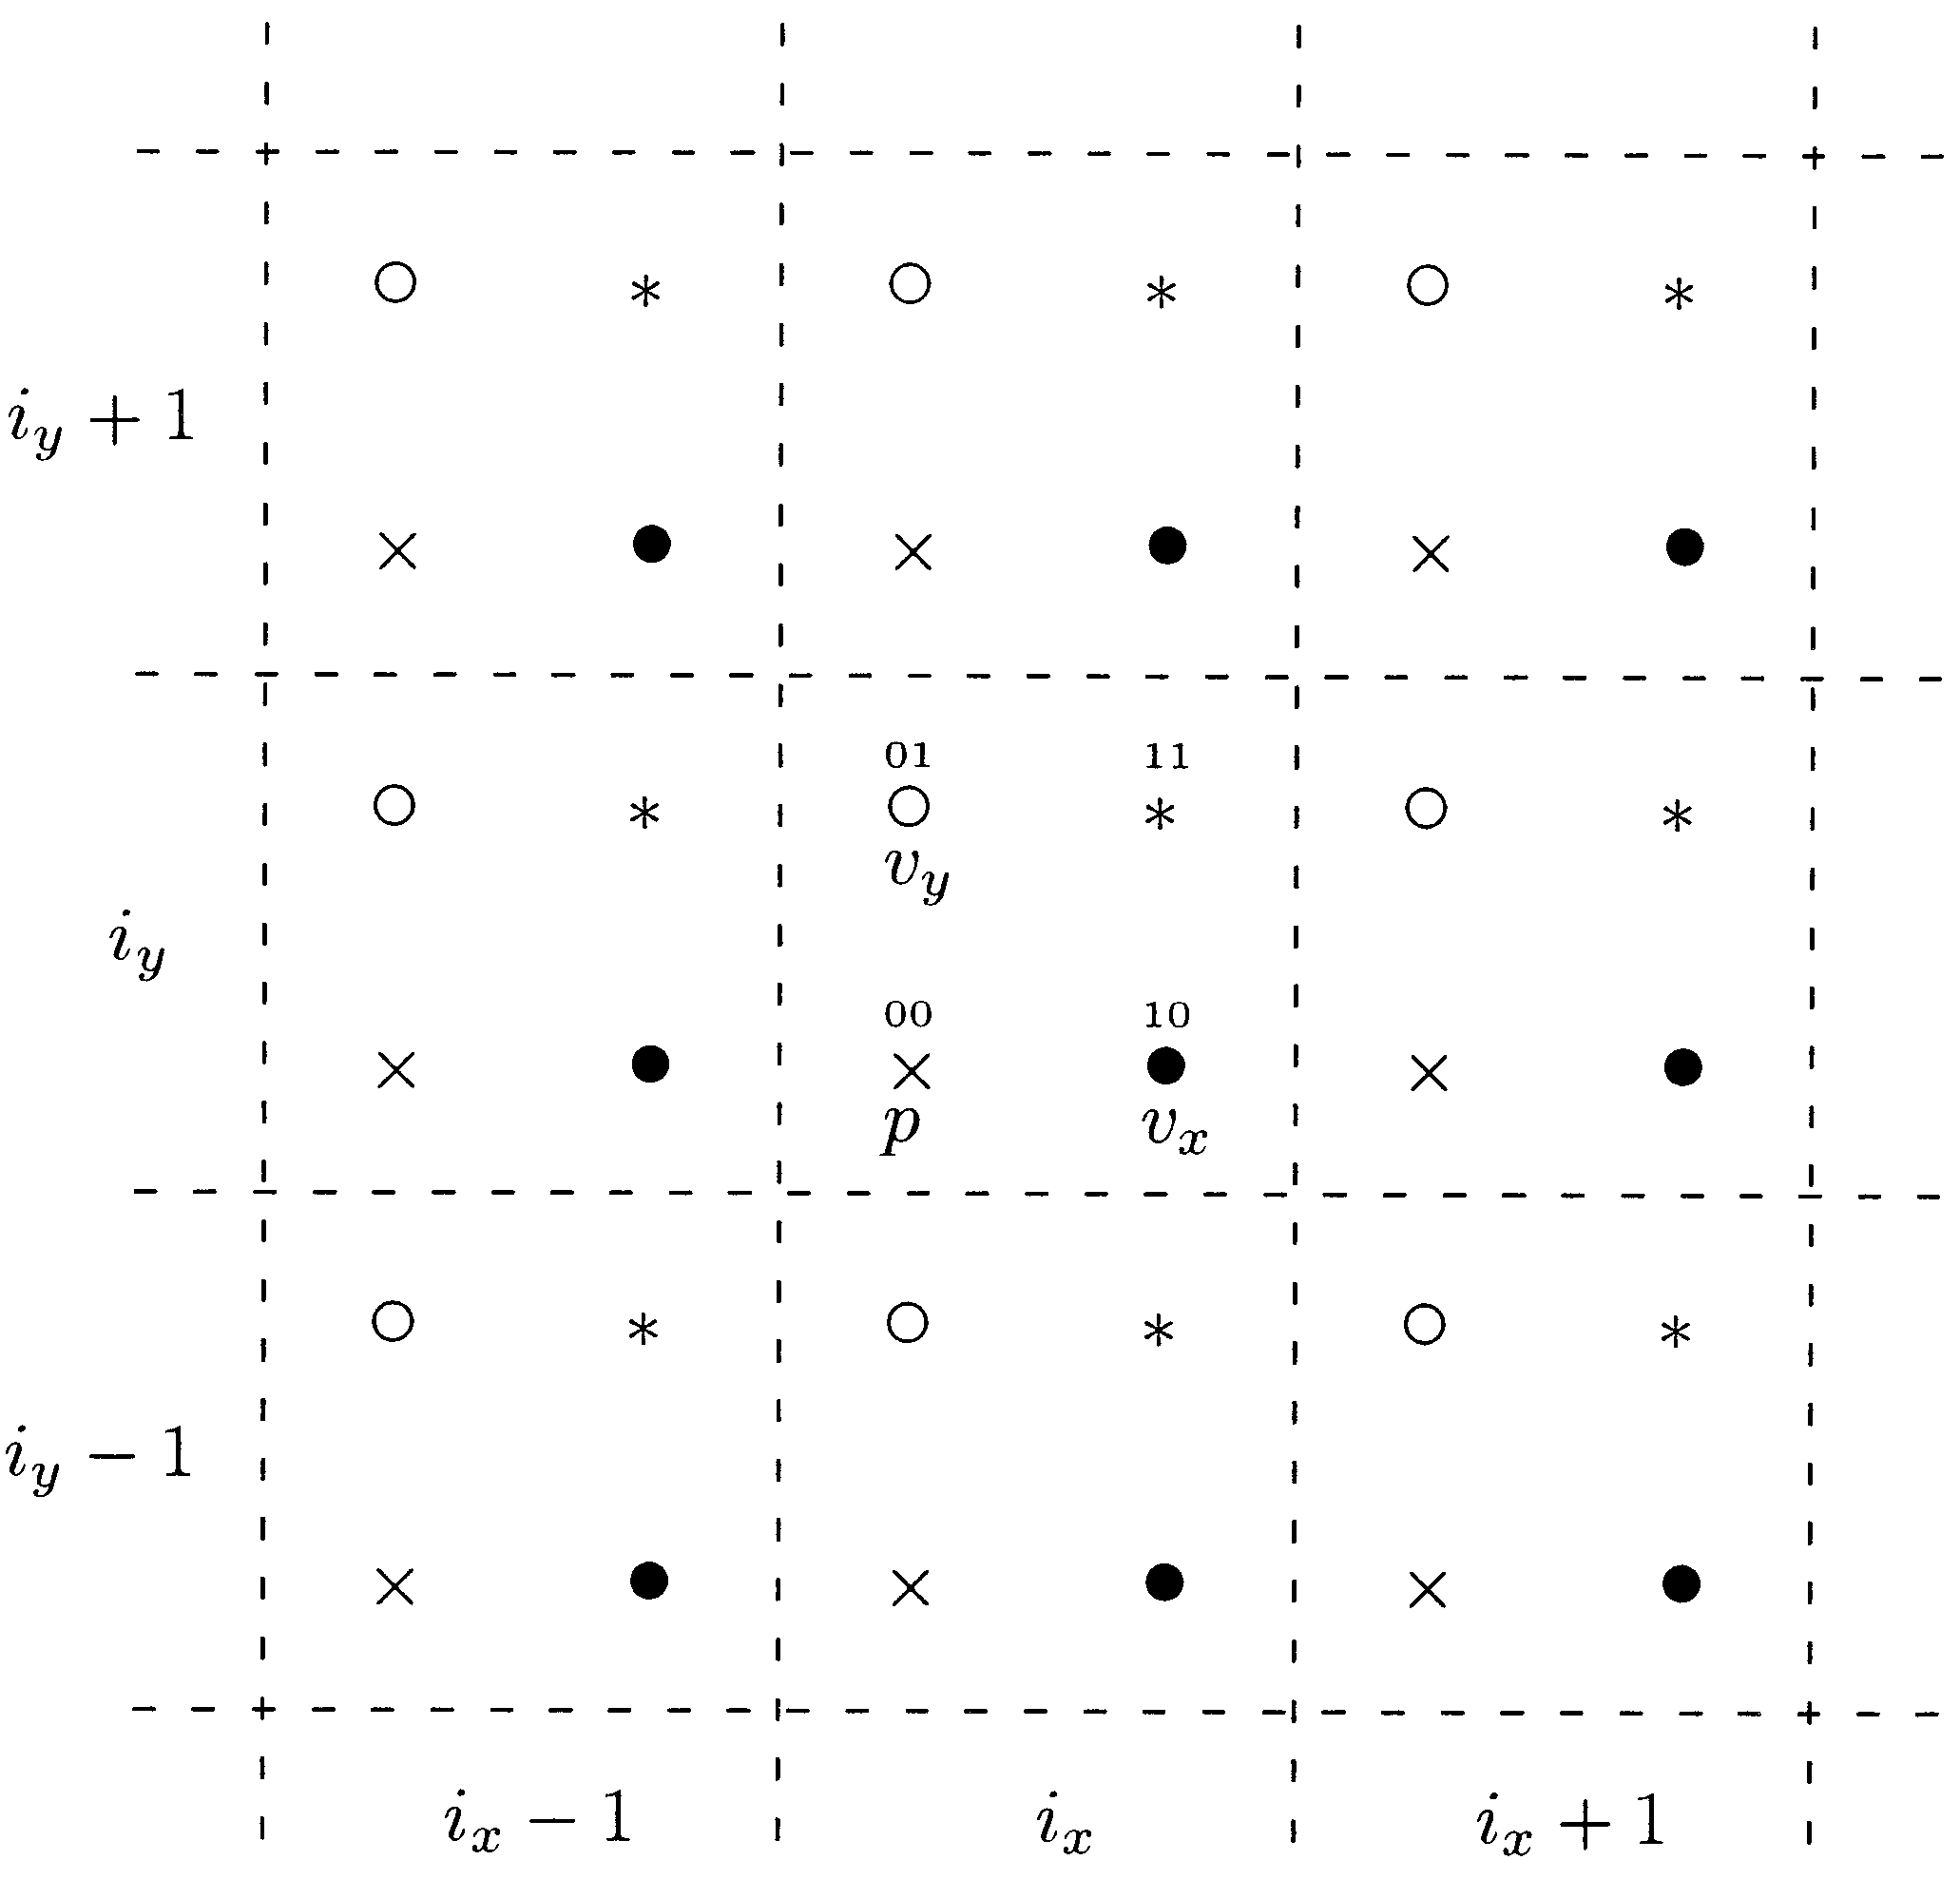
\includegraphics[width=0.4\textwidth]{figures/stag1}
	\caption{The placement of the pressure and velocity variables on a 2D staggered grid. The dashed squares denote the cells. The figure is taken form \citet{Lautrup}.}
	\label{fig:1}
\end{figure}
With this information in hand equation \eqref{o1} can be discretized as follows
\begin{equation}
	\rho \begin{bmatrix}
		\frac{v_x[i_x,i_y,i_z,t+1]-v_x[i_x,i_y,i_z,t]}{\Delta t}\\
		\frac{v_y[i_x,i_y,i_z,t+1]-v_y[i_x,i_y,i_z,t]}{\Delta t}\\
		\frac{v_z[i_x,i_y,i_z,t+1]-v_z[i_x,i_y,i_z,t]}{\Delta t}\\
	\end{bmatrix}=\begin{bmatrix}
		f_x[i_x,i_y,i_z,t]-\frac{p[i_x+1,i_y,i_z,t]-p[i_x,i_y,i_z,t]}{\Delta x}\\
		f_y[i_x,i_y,i_z,t]-\frac{p[i_x,i_y+1,i_z,t]-p[i_x,i_y,i_z,t]}{\Delta y}\\
		f_z[i_x,i_y,i_z,t]-\frac{p[i_x,i_y,i_z+1,t]-p[i_x,i_y,i_z,t]}{\Delta z}\\
	\end{bmatrix}.
\end{equation}
Note that the first equation is located on the same grid-point as $v_x$, the second on the same grid-point as $v_y$ and the third on the same grid-point as $v_z$. From the derivative of the pressure it is clear that the $v_z$ point must be orthogonal to the pressure point\footnote{$v_z$ is out of the screen on figure \ref{fig:1} since $i_z+1$ minus $i_z$ must land on the pressure point.}. This information is important since the different components of the generalized force is forced to be located on the grid-points corresponding to the rest of the given equation. Writing out the generalized force
\begin{equation}
	\vec{f}=\begin{bmatrix}
		f_{b,x}-\rho\big(v_x\frac{\partial v_x}{\partial x}+v_y\frac{\partial v_x}{\partial y}+v_z\frac{\partial v_x}{\partial z}\big)+\eta \big[\frac{\partial^2 v_x}{\partial x^2}+\frac{\partial^2 v_x}{\partial y^2}+\frac{\partial^2 v_x}{\partial z^2}+(\frac{1}{3}+\frac{\zeta}{\eta})\big(\frac{\partial^2 v_x}{\partial x^2}+\frac{\partial^2 v_y}{\partial x\partial y}+\frac{\partial^2 v_z}{\partial x\partial z}\big)\big]\\
		f_{b,y}-\rho\big(v_x\frac{\partial v_y}{\partial x}+v_y\frac{\partial v_y}{\partial y}+v_z\frac{\partial v_y}{\partial z}\big)+\eta \big[\frac{\partial^2 v_y}{\partial x^2}+\frac{\partial^2 v_y}{\partial y^2}+\frac{\partial^2 v_y}{\partial z^2}+(\frac{1}{3}+\frac{\zeta}{\eta})\big(\frac{\partial^2 v_x}{\partial y\partial x}+\frac{\partial^2 v_y}{\partial y^2}+\frac{\partial^2 v_z}{\partial y\partial z}\big)\big]\\
		f_{b,z}-\rho\big(v_x\frac{\partial v_z}{\partial x}+v_y\frac{\partial v_z}{\partial y}+v_z\frac{\partial v_z}{\partial z}\big)+\eta \big[\frac{\partial^2 v_z}{\partial x^2}+\frac{\partial^2 v_z}{\partial y^2}+\frac{\partial^2 v_z}{\partial z^2}+(\frac{1}{3}+\frac{\zeta}{\eta})\big(\frac{\partial^2 v_x}{\partial z\partial x}+\frac{\partial^2 v_y}{\partial z\partial y}+\frac{\partial^2 v_z}{\partial z^2}\big)\big]\\
	\end{bmatrix}.
\end{equation}
In order for the advective term ($\propto \rho$) to belong to the same point as $v_x$, the derivative must be averaged over the adjacent points, meaning e.g.
\begin{equation}
	\begin{split}
		&v_x\frac{\partial v_x}{\partial x} \rightarrow  v_x[i_x,i_y,i_z,t]\frac{v_x[i_x+1,i_y,i_z,t]-v_x[i_x-1,i_y,i_z,t]}{2\Delta x},\\
		&v_y\frac{\partial v_x}{\partial y}\rightarrow  \braket{v_y}\frac{v_x[i_x,i_y+1,i_z,t]-v_x[i_x,i_y-1,i_z,t]}{2\Delta y},\\
		&v_z\frac{\partial v_x}{\partial z}\rightarrow  \braket{v_z}\frac{v_x[i_x,i_y,i_z+1,t]-v_x[i_x,i_y,i_z-1,t]}{2\Delta z},\\
	\end{split}
\end{equation}
where
\begin{equation}
	\begin{split}
		&\braket{v_y}\equiv \frac{v_y[i_x,i_y,i_z,t]+v_y[i_x,i_y-1,i_z,t]+v_y[i_x+1,i_y,i_z,t]+v_y[i_x+1,i_y-1,i_z,t]}{4},\\
		&\braket{v_z}\equiv \frac{v_z[i_x,i_y,i_z,t]+v_z[i_x,i_y,i_z-1,t]+v_z[i_x,i_y+1,i_z,t]+v_z[i_x,i_y+1,i_z-1,t]}{4}.\\
	\end{split}
\end{equation}
The second derivatives are with respect to the same variable are naturally located on the same point e.g.
\begin{equation}
	\begin{split}
		&\frac{\partial^2 v_x}{\partial x^2} \rightarrow  \frac{v_x[i_x+1,i_y,i_z,t]+v_x[i_x-1,i_y,i_z,t]-2v_x[i_x,i_y,i_z,t]}{\Delta x^2},\\
		&\frac{\partial^2 v_x}{\partial y^2}\rightarrow   \frac{v_x[i_x,i_y+1,i_z,t]+v_x[i_x,i_y-1,i_z,t]-2v_x[i_x,i_y,i_z,t]}{\Delta x^2},\\
		&\frac{\partial^2 v_x}{\partial z^2}\rightarrow  \frac{v_x[i_x,i_y,i_z+1,t]+v_x[i_x,i_y,i_z-1,t]-2v_x[i_x,i_y,i_z,t]}{\Delta x^2}.\\
	\end{split}
\end{equation}
For the divergence term it is less simple for the terms with mixed derivatives. Here the average of both derivatives must be used such that
\begin{equation}
	\begin{split}
		\frac{\partial^2 v_x}{\partial x\partial y} \rightarrow \frac{1}{4\Delta x \Delta y}\bigg(&v_x[i_x+1,i_y+1,i_z,t]+v_x[i_x-1,i_y-1,i_z,t]\\
		&-v_x[i_x+1,i_y-1,i_z,t]-v_x[i_x-1,i_y+1,i_z,t]\bigg),\\
	\end{split}
\end{equation}                           
\begin{equation}
	\begin{split}
		\frac{\partial^2 v_x}{\partial x\partial z} \rightarrow \frac{1}{4\Delta x \Delta z}\bigg(&v_x[i_x+1,i_y,i_z+1,t]+v_x[i_x-1,i_y,i_z-1,t]\\
		&-v_x[i_x+1,i_y,i_z-1,t]-v_x[i_x-1,i_y,i_z-1,t]\bigg),\\
	\end{split}
\end{equation}   
The specific approach (read programming) to obtaining a solution from the discretized equations of motion depend on the physical scenario under consideration and potential simplifying assumptions that can be made.

\begin{example}
	The perhaps most used simplification of Navier-Stokes equations is to take the fluid to be incompressible ($\rho\simeq const$). Taking the density to be constant means the velocity field will be divergence-less. To see this, consider a material particle riding along with the flow in a fluid. At time $t+\delta t$ the particle will be displaced by an amount $\vec{x}+v(\vec{x},t)\delta t$. The change in mass density during this time
	\begin{equation}
		\begin{split}
			\delta \rho &=\rho(\vec{x}+v(\vec{x},t)\delta t,t+\delta t)-\rho(\vec{x},t)\\
			&= v_{x}\delta t\frac{\partial \rho (\vec{x},t)}{\partial x}+v_{y}\delta t\frac{\partial \rho (\vec{x},t)}{\partial y}+v_{z}\delta t\frac{\partial \rho (\vec{x},t)}{\partial z}+\delta t\frac{\partial \rho (\vec{x},t)}{\partial t}+\mathcal{O}(\delta t^2)\\
			&=\bigg(\frac{\partial \rho}{\partial t}+(\vec{v}\cdot \vec{\nabla})\rho\bigg)\delta t.
		\end{split}
	\end{equation}
	Dividing by $\delta t$ reveals the rate of change of density as seen from the material particle, i.e. the material derivative of the density
	\begin{equation}
		\frac{D \rho}{Dt}=\frac{\partial \rho}{\partial t}+(\vec{v}\cdot \vec{\nabla})\rho.
		\label{one}
	\end{equation}
	Imposing conservation of mass means
	\begin{equation}
		\frac{\partial \rho}{\partial t}+\vec{\nabla}(\rho\vec{v})=0,
		\label{two}
	\end{equation}
	with $\vec{\nabla}(\rho\vec{v})=(\vec{v}\cdot \vec{\nabla})\rho+\rho\vec{\nabla}\cdot \vec{v}$. Combining equation \eqref{one} and \eqref{two} reveals
	\begin{equation}
		\frac{D \rho}{Dt}+\rho\vec{\nabla}\cdot \vec{v}=0.
		\label{three}
	\end{equation}
	From equations \eqref{three} and \eqref{one} it is clear that by taking $\rho=const$ the material derivative vanish and by extension it is required that the velocity field is divergence-free ($\vec{\nabla}\cdot \vec{v}=0$). This information can be used to simplify the Navier-Stokes equations. Taking the divergence of equation \eqref{o1}
	\begin{equation}
		\vec{\nabla}^2p=\vec{\nabla}\cdot\vec{f}\equiv s,
		\label{o3}
	\end{equation}
	where $s$ abbreviates "source". 
\end{example}



\chapter{Analytical Mechanics}
Analytical mechanics, derived primarily by Joseph-Louis Lagrange and William Rowan Hamilton in the late 1700's and early 1800's, is a framework equivalent to Newtonian mechanics for conservative forces\footnote{The Lagrangian formalism utilizes the potential energy function which is only defined for a conservative force field. Non-conservative forces can be incorporated with much difficulty however.}. The framework consists of three equivalent schemes; Lagrangian mechanics, Hamiltonian mechanics and Hamilton-Jacobi mechanics. These schemes provide the foundation for three of the quantum mechanical formalisms. These generalizations will be considered in chapter \ref{chp:4}. 
\begin{figure}[h]
	\captionsetup{width=1\textwidth}
	\centering
	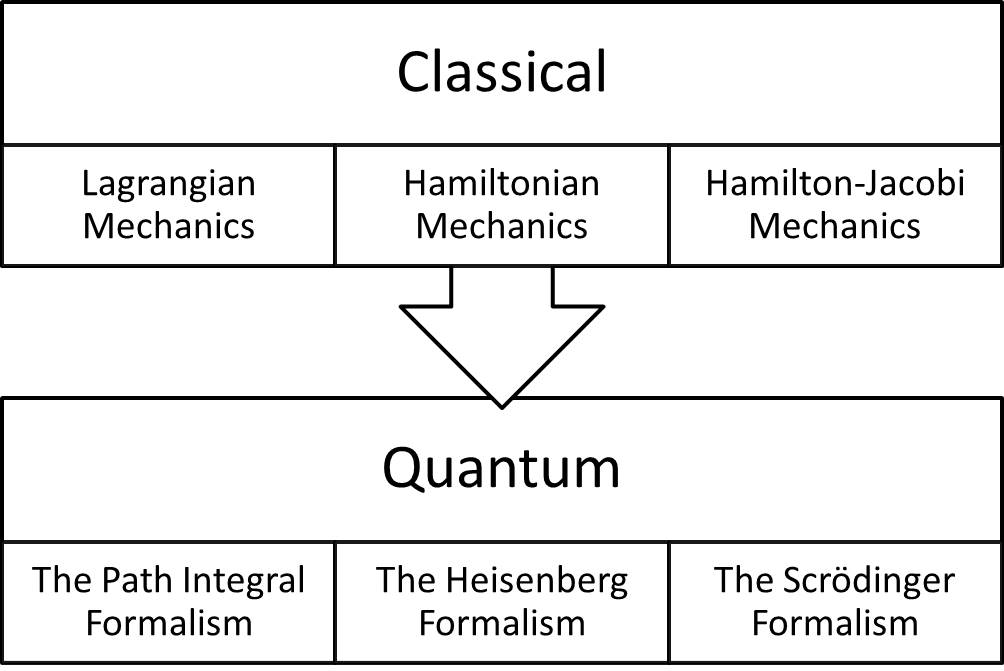
\includegraphics[width=0.5\textwidth]{figures/Billede1}
\end{figure}
The schemes of analytical mechanics was derived with the intention to investigate the fundamental processes in nature that led to Newtons laws. This quest was by and large successful and significant physical insight can be gained by studying the schemes of analytical mechanics. 

\section{Lagrangian Mechanics}
The Lagrangian formalism was introduced by Joseph-Luis Lagrange in 1788 ($\sim100$ years after Newtons laws). Back in the days scientists were concentrated on finding a more general formulation of the principles of physics - Compared to the Newtonian formalism. Newtons laws provide instructions to acquire the laws of motion, but they do not provide an explanation as to \emph{why} the laws are in the way they are. An explanation as to why came from developing Lagrangian mechanics; everything in physics derives from the principle of least action! 

\subsection*{The principle of least action}
Consider a generic physical system which has an instantaneous configuration described by the values of $n$ generalized coordinates, $\bar{q}\equiv(q_1, q_2,...q_n)$. Because the generalized coordinates determine the configuration of the system, they span what is called \emph{configuration space}\index{Configuration space}, and the physical state of the system is given as a point in this $n$-dimensional hyperspace~\citep{Goldstein}. As time progresses, the state of the general physical system will change. For the generalized coordinates, this change of state results in the point tracing out a line (or path), called the path of motion, in configuration space. Which path of motion the system will take is described by \emph{Hamiltons principle}\index{Hamiltons principle}\index{Principle of least action}, also called the principle of stationary (or least) action. 

\paragraph{The principle of stationary action:} \emph{The motion of the system from time $t_1$ to $t_2$ is such that the action ($S$) is extremized (minimized most often)\footnote{The reason why the system traces the path in configuration space that corresponds to the minimized action can be explained from quantum mechanics and the path integral scheme. In the path integral scheme the transition probability is given in terms of the path integral of $e^{\frac{iS}{\hbar}}$ (SI units). In the classical limit ($\hbar\Rightarrow 0$ the exponential will fluctuate wildly and all contributions besides those which corresponds to a minimized action will cancel cf. the random phase principle.)}}\newline

The action\index{Action, classical} is defined by the integral~\citep{Sannino}
\begin{equation}
	S\big[\bar{q},\dot{\bar{q}}, t_1,t_2\big]=\int_{t_1}^{t_2}L\big(\bar{q}(t),\dot{\bar{q}}(t),t\big)dt,
	\label{action}
\end{equation} 
where the square brackets indicate that the action is a \emph{functional} rather than a \emph{function}\footnote{A function is a rule that assigns a unique element, $f(x)$, from a set to each value, $x$, in another set; a function takes in a number and produces a number. A functional, on the other hand, associates a vector valued function with a real number.}. The function $L$ is the \emph{Lagrangian}\index{Lagrangian, definition} and is defined as
\begin{equation}
	L\big(\bar{q}(t),\dot{\bar{q}}(t),t\big)=T\big(\dot{\bar{q}}(t)\big)-V\big(\bar{q}(t),t\big),
	\label{Lagrangeian}
\end{equation} 
where $T$ is the kinetic energy of the system and $V$ is the potential energy of the system. 

\subsubsection*{The Euler-Lagrange equation}
By minimizing the action of equation \eqref{action} the master equation of Lagrangian mechanics, the Euler-Lagrange equation, is obtained. Consider a variation of the action:
\begin{equation}
	\begin{split}
		\delta S\big[\bar{q},\dot{\bar{q}}, t_1,t_2\big]
		&=\delta\int_{t_1}^{t_2} L\big(\bar{q}(t),\dot{\bar{q}}(t),t\big)dt\\
		&=\int_{t_1}^{t_2}\sum_{j=1}^{n}\bigg(\frac{\partial L\big(\bar{q}(t),\dot{\bar{q}}(t),t\big)}{\partial q_j(t)}\delta q_j(t)+\frac{\partial L\big(\bar{q}(t),\dot{\bar{q}}(t),t\big)}{\partial \dot{q}_j(t)}\delta \dot{q}_j(t)\bigg)dt\\
		&=\int\sum_{j}\frac{\partial L\big(\bar{q}(t),\dot{\bar{q}}(t),t\big)}{\partial q_j(t)}\delta q_j(t)dt+\int\sum_{j}\frac{\partial L\big(\bar{q}(t),\dot{\bar{q}}(t),t\big)}{\partial \dot{q}_j(t)}\delta \dot{q}_j(t)dt,
	\end{split}
	\label{lag3}
\end{equation} 
where $\dot{\bar{q}}(t)=(\dot{q}_1(t), \dot{q}_2(t),\dots\dot{q}_n(t))$\normalsize and $\bar{q}(t)=(q_1(t), q_2(t),\dots q_n(t))$\normalsize. The last term is evaluated by partial integration
\begin{equation}
	\begin{split}
		\int\sum_{j}\frac{\partial L\big(\bar{q}(t),\dot{\bar{q}}(t),t\big)}{\partial \dot{q}_j(t)}\delta \dot{q}_j(t)dt&=\int\sum_{j}\frac{d}{dt}\bigg(\frac{\partial L\big(\bar{q}(t),\dot{\bar{q}}(t),t\big)}{\partial \dot{q}_j(t)}\delta q_j(t)\bigg)dt\\
		&\quad-\int\sum_{j}\frac{d}{dt}\bigg(\frac{\partial L\big(\bar{q}(t),\dot{\bar{q}}(t),t\big)}{\partial \dot{q}_j(t)}\bigg)\delta q_j(t)dt,
	\end{split}
	\label{lag2}
\end{equation} 
where
\begin{equation}
	\int_{t_1}^{t_2}\sum_{j}\frac{d}{dt}\bigg(\frac{\partial L\big(\bar{q}(t),\dot{\bar{q}}(t),t\big)}{\partial \dot{q}_j(t)}\delta q_j(t)\bigg)dt=\sum_{j}\frac{\partial L\big(\bar{q}(t),\dot{\bar{q}}(t),t\big)}{\partial \dot{q}_j(t)}\delta q_j(t)\bigg|_{t_1}^{t_2}=0.
	\label{lag1}
\end{equation} 
Equation \eqref{lag1} vanish by taking the endpoints of the path to be fixed, i.e. $\delta q_j(t_1)=\delta q_j(t_2)=0$ is taken as boundary conditions. By using equation \eqref{lag1} in equation \eqref{lag2} and the result in equation \eqref{lag3} the variation in the action can be written as
\begin{equation}
	\delta S\big[\bar{q},\dot{\bar{q}}, t_1,t_2\big]=\int\sum_{j}\bigg(\frac{\partial L\big(\bar{q}(t),\dot{\bar{q}}(t),t\big)}{\partial q_j(t)}-\frac{d}{dt}\bigg(\frac{\partial L\big(\bar{q}(t),\dot{\bar{q}}(t),t\big)}{\partial \dot{q}_j(t)}\bigg) \bigg)\delta q_j(t)dt.
	\label{lag4}
\end{equation} 
To minimize the action (find a minimum in $S$), the variation (equation \eqref{lag4}) must vanish. In order for the variation to vanish for an arbitrary $\delta q_j(t)$, the remaining part of the integrand must always be zero. That is
\begin{equation}
	\frac{\partial L\big(\bar{q}(t),\dot{\bar{q}}(t),t\big)}{\partial q_j(t)}-\frac{d}{dt}\bigg(\frac{\partial L\big(\bar{q}(t),\dot{\bar{q}}(t),t\big)}{\partial \dot{q}_j(t)}\bigg)=0. 
	\label{lag5}
\end{equation} 
Equation \eqref{lag5} is called the \emph{Euler-Lagrange} equation\index{Euler-Lagrange equation}. It is often written in the less detailed form
\begin{equation}
	\frac{\partial L}{\partial q_j}-\frac{d}{dt}\bigg(\frac{\partial L}{\partial \dot{q}_j}\bigg)=0. 
	\label{EL}
\end{equation} 
The Euler-Lagrange equation is a second order differential equation in time, and from it the equations of motion can be determined by specifying, and inserting, the Lagrangian. Thus, the Euler-Lagrange equation is equivalent to Newtonian dynamics, but instead of postulating a series of laws, the equations of motions are derived from the assumption that the path of the system in configuration space is the path of least action. This provides profound, new physical insight into the machinery of nature.
\begin{example}
	\emph{Determine and solve the EOM for a movable, simple pendulum.}\newline
	
	The movable, simple pendulum consist of two particles; one particle ($m_1$) is confined to a horizontal movement, whereas another particle ($m_2$) is attached to the first via a (massless) string, and is free to swing back and forth - See figure \ref{fig:sphere}.
	\begin{figure}[h]
		\captionsetup{width=1\textwidth}
		\centering
		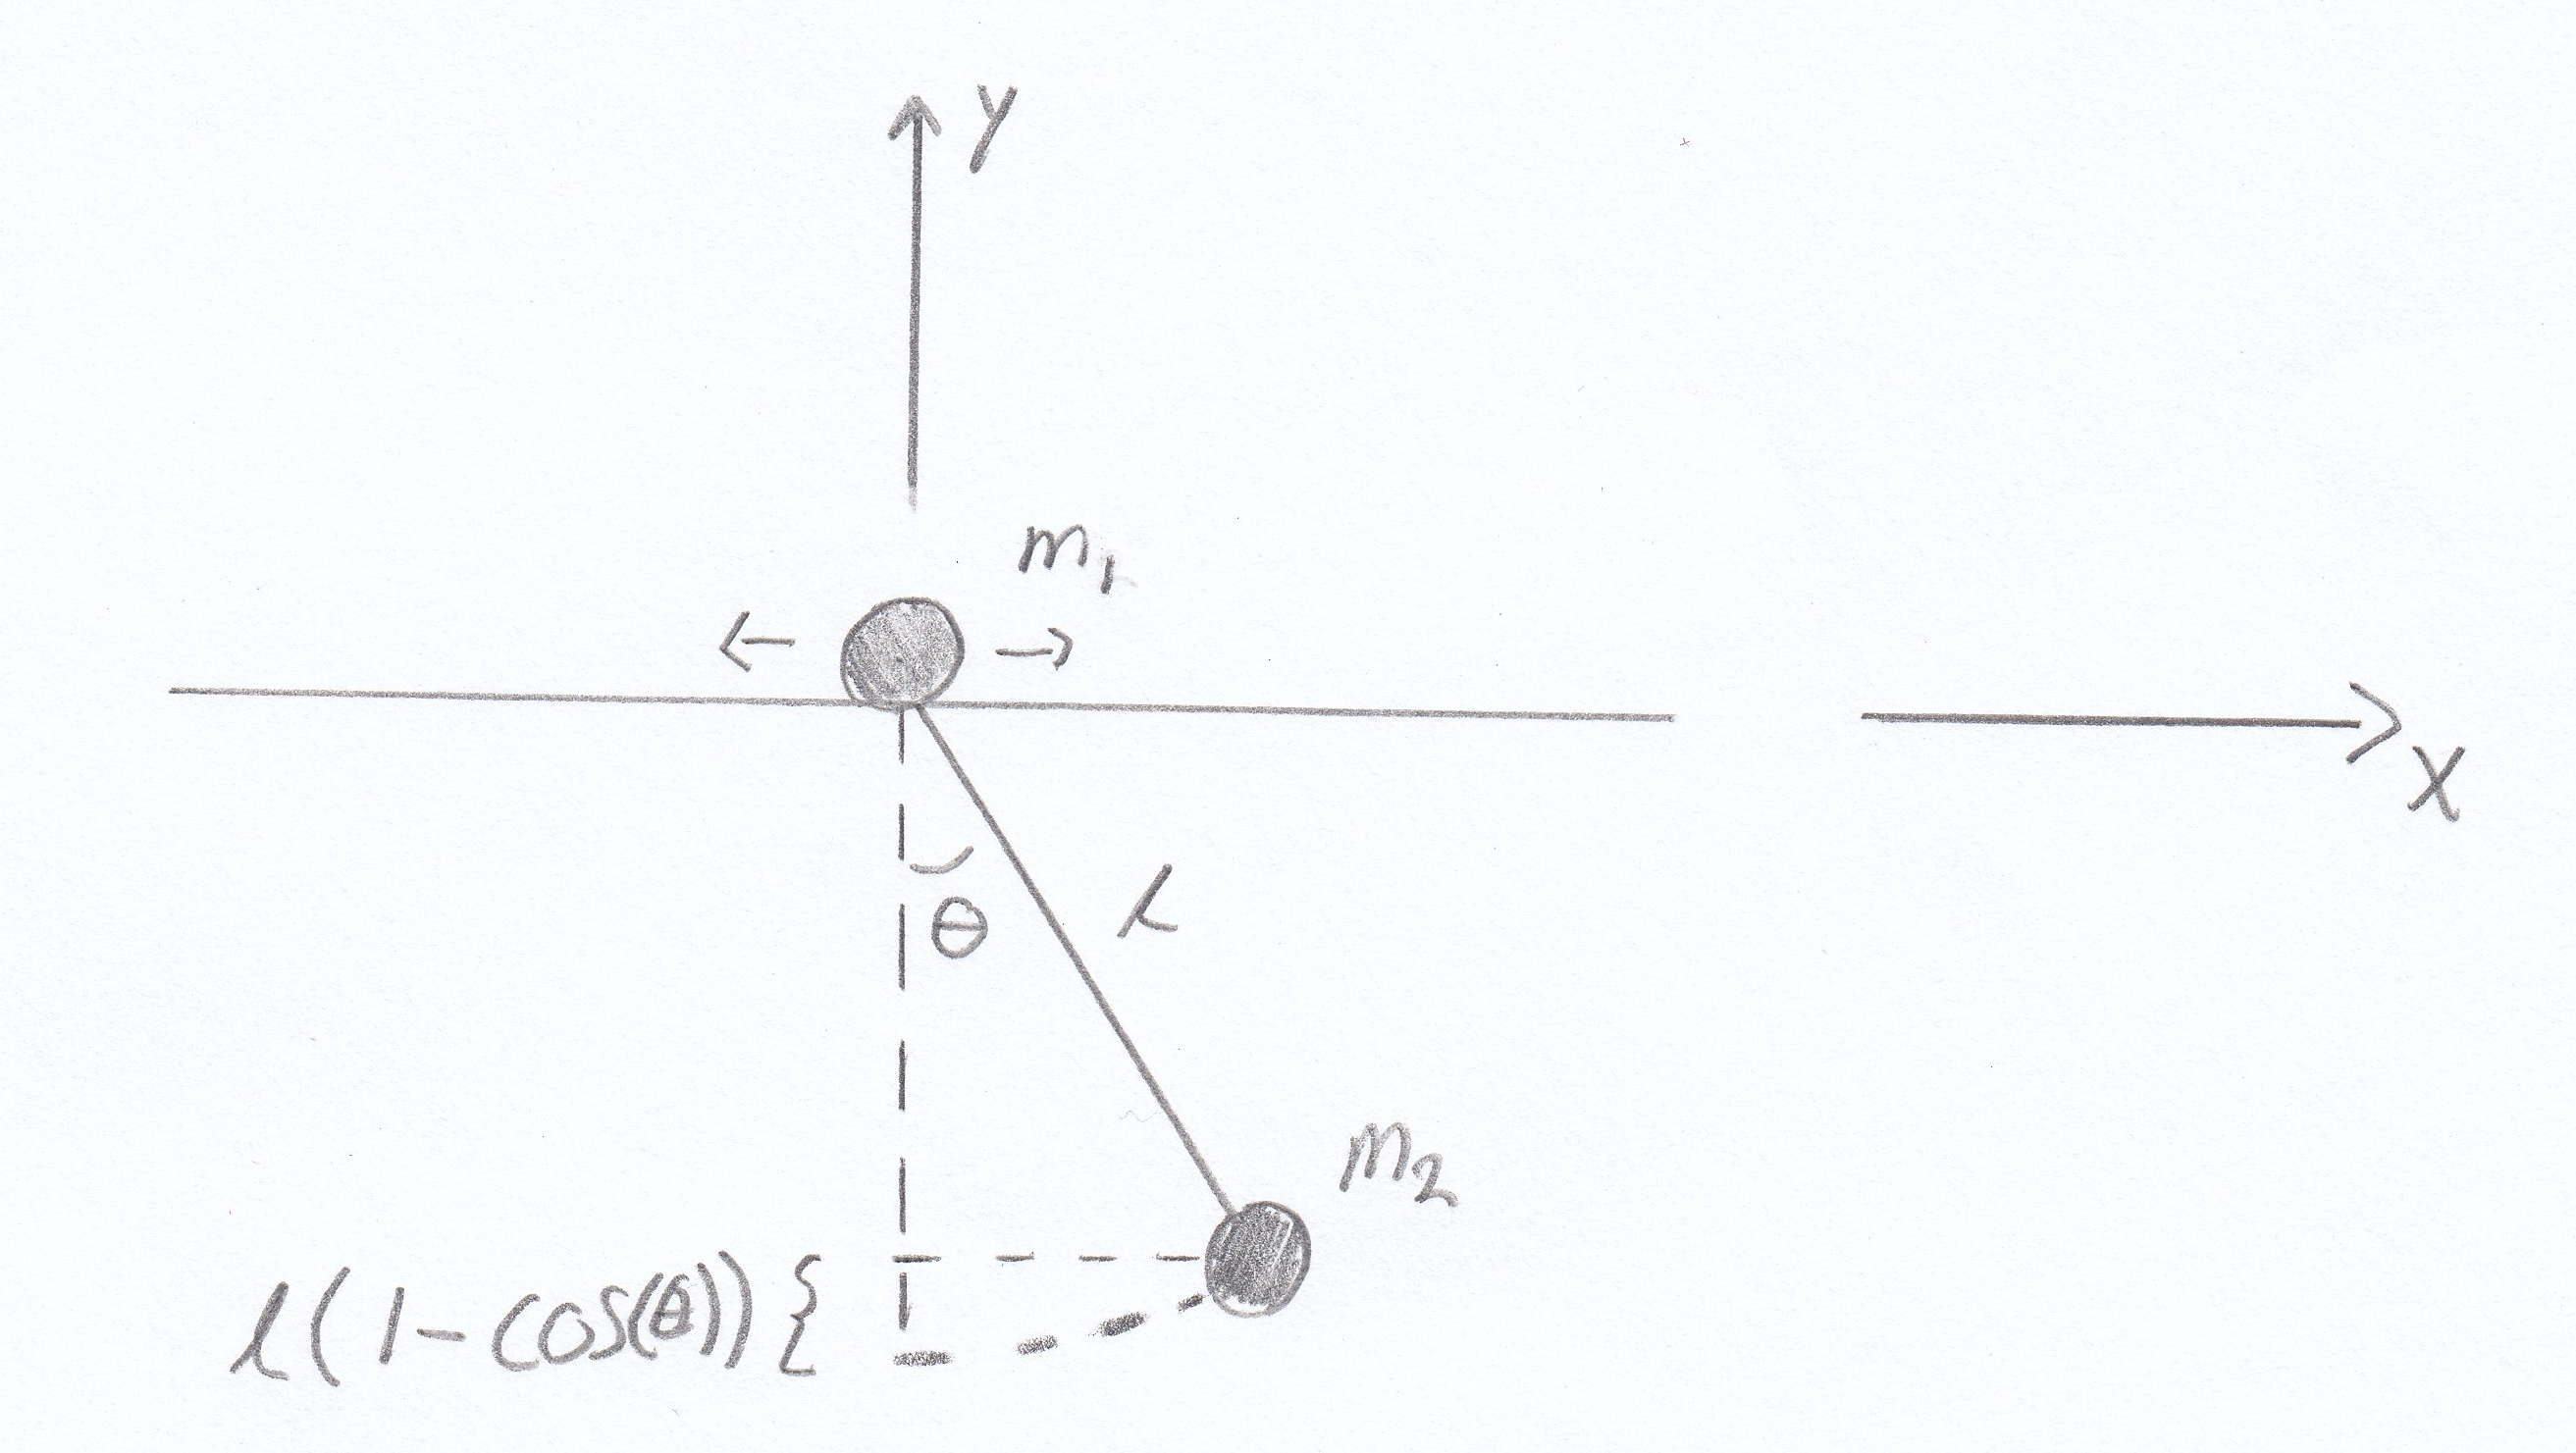
\includegraphics[width=0.5\textwidth]{figures/sphere}
		\caption{The spherical pendulum with spherical coordinates.}
		\label{fig:sphere}
	\end{figure}
	In terms of the, from the figure, defined coordinate system, the coordinates are given by
	\begin{equation}
		x_1=x_1, \quad y_1=0,
	\end{equation} 
	\begin{equation}
		x_2=x_1+lsin(\theta), \quad y_2=-lcos(\theta),
	\end{equation} 
	where the minus sign in $y_2$ is there because the second particle is defined to swing at negative $y$. For the potential energy in the Lagrangian the relevant distance\footnote{So that the potential energy is positive when the mass is displaced from equilibrium.} is the vertical displacement from equilibrium $(l-y_2)$, so the Lagrangian is given by
	\begin{equation}
		L=\frac{1}{2}m_1\dot{x}_1^2+\frac{1}{2}m_2(\dot{x}_2^2+\dot{y}_2^2)-m_2gl(1-cos(\theta)).
	\end{equation} 
	The velocity of the second particle is
	\begin{equation}
		\begin{split}
			\dot{x}_2^2+\dot{y}_2^2&=\dot{x}_1^2+2\dot{x}_1lcos(\theta)\dot{\theta}+l^2cos(\theta)^2\dot{\theta}^2+l^2sin(\theta)^2\dot{\theta}^2\\
			&=\dot{x}_1^2+l^2\dot{\theta}^2+2l\dot{x}_1\dot{\theta}cos(\theta).
		\end{split}
	\end{equation} 
	So
	\begin{equation}
		L=\frac{1}{2}m_1\dot{x}_1^2+\frac{1}{2}m_2(\dot{x}_1^2+l^2\dot{\theta}^2+2l\dot{x}_1\dot{\theta}cos(\theta))-m_2gl(1-cos(\theta)).
	\end{equation} 
	Using $x_1$ and $\theta$ as generalized coordinates, the EOM can be found from the Euler-Lagrange equation
	\begin{equation}
		\underbrace{\frac{\partial L}{\partial x_1}}_{=0}-\frac{d}{dt}\bigg(\frac{\partial L}{\partial \dot{x}_1}\bigg)=0\Rightarrow \dot{x}_1(m_1+m_2)+m_2lcos(\theta)\dot{\theta}=const=p_{x_1},
	\end{equation} 
	\begin{equation}
		\begin{split}
			0&=\frac{\partial L}{\partial \theta}-\frac{d}{dt}\bigg(\frac{\partial L}{\partial \dot{\theta}}\bigg)\Rightarrow -m_2lsin(\theta)(\dot{x}_1\dot{\theta}+g)-m_2l(l\ddot{\theta}+\ddot{x}_1cos(\theta)-\dot{x}_1\dot{\theta}sin(\theta))=0.
		\end{split}
	\end{equation} 
	Two of the terms ($\dot{x}_1\dot{\theta}$) cancel, so
	\begin{equation}
		m_2l^2\ddot{\theta}+m_2glsin(\theta)+m_2l\ddot{x}_1cos(\theta)=0.
	\end{equation} 
	Eliminate $\ddot{x}_1$ from the above equation by using the Euler-Lagrange equation for $x_1$. Hereby
	\begin{equation}
		\begin{split}
			0&=\ddot{x}_1(m_1+m_2)+m_2l(cos(\theta)\ddot{\theta}-sin(\theta)\dot{ \theta}^2)\\
			&\Rightarrow \ddot{x}_1=\frac{m_2l}{m_1+m_2}(\dot{\theta}^2sin(\theta)-\ddot{\theta}cos(\theta)).
		\end{split}
	\end{equation} 
	So
	\begin{equation}
		m_2l^2\ddot{\theta}-\frac{m_2^2l^2cos(\theta)^2}{m_1+m_2}\ddot{\theta}+\frac{m_2^2l^2cos(\theta)sin(\theta)}{m_1+m_2}\dot{\theta}^2+m_2lgsin(\theta)=0.
	\end{equation} 
	This is in general difficult to solve, so I consider the  limiting cases
	\begin{equation}
		m_2\gg m_1 \wedge \theta=\text{small:}\quad \dot{\theta}^2+\frac{g}{l}\approx 0 \Rightarrow \theta\approx
		\sqrt{-\frac{g}{l}}t+A.
	\end{equation} 
	Since $g>0$ the above EOM is complex. This makes sense physically since if $m_2\gg m_1$, $m_2$ will drag $m_1$ along and no swinging motion at small angles will occur. Hence, $m_2\gg m_1$ and $\theta=\text{small}$ ar incompatible approximations. Instead I consider $m_2\ll m_1 \wedge \theta=\text{small}$. This corresponds to a small mass swinging fro a large mass. In the limit of large $m_1$ this should simplify to the simple pendulum since at small angles $m_1$ should not move. Indeed this is what I find
	\begin{equation}
		m_2\ll m_1 \wedge \theta=\text{small:}\quad \ddot{\theta}+\frac{g}{l}\theta\approx 0 \Rightarrow \theta\approx \theta_0cos\bigg(\sqrt{\frac{g}{l}}t\bigg).
	\end{equation} 
\end{example}
Since the equations of motion falls out directly from the Euler-Lagrange equation, and since the equations of motion in Newtonian mechanics are directly related to the rate of change of momentum, it is no surprise that the momentum, and the rate of change of momentum, is related to the Euler-Lagrange equation. However, since the Euler-Lagrange equation deals with generalized coordinates, the momentum that is referred to is not necessarily the linear momentum. If for example a system of polar coordinates are considered, the momentum derived from the Euler-Lagrange equation is the angular momentum. Thus, the momentum related to the Euler-Lagrange equation is called the canonical momentum conjugate \index{Conjugate momentum} to the generalized coordinate $q_j$, $p_j$, and it is defined as
\begin{equation}
	p_j=\frac{\partial L}{\partial \dot{q}_j}.
	\label{conj. momentum}
\end{equation} 
By using this definition in the Euler-Lagrange-equation, it directly follows that
\begin{equation}
	\dot{p}_j=\frac{\partial L}{\partial q_j}.
	\label{diff. conj. momentum}
\end{equation} 
Using equation \eqref{conj. momentum} and \eqref{diff. conj. momentum} in the Euler-Lagrange equation it is clear that it (the Euler-Lagrange equation) stipulates $\dot{p}-\dot{p}=0$, which is indeed the case. Memo-technically this is a good thing to remember because one of the quantities are to be differentiated wrt. time, so if the equation must read $\dot{p}-\dot{p}=0$ it can be deduced that $\frac{\partial L}{\partial \dot{q}_j}$, which is to be differentiated wrt. time in the Euler-Lagrange equation, must equal $p$. From equation \eqref{diff. conj. momentum} it follows that if the Lagrangian does not depend on a given coordinate, $q_j$, the corresponding momentum is conserved; $\frac{\partial p_j}{\partial t}=0\Rightarrow p_j=\mbox{conserved}$. An alternative way to formulate the principle of conserved quantities is via Noethers theorem\index{Noethers theorem, classical mechanics}.

\paragraph{Noethers theorem:}\emph{Transformations under which the Lagrangian is unchanged have a conserved quantity associated to them.}


\begin{example}
	Consider a translational invariant physical system described by the Lagrangian $L(x_i,\dot{x}_i)$. A constant displacement of $x_i$ will leave the Lagrangian invariant. Hence, the Lagrangian is invariant under the transformation
	\begin{equation}
		x_i\Rightarrow x_i+\delta x,
	\end{equation} 
	where $\delta x$ is a constant. The change in the Lagrangian under this transformation can be described as
	\begin{equation}
		\delta L=\frac{\partial L}{\partial x_i}\delta x_i+\frac{\partial L}{\partial \dot{x}_i}\delta\dot{x}_i=\delta x\frac{\partial L}{\partial x_i}=\delta x\frac{d}{dt}\bigg(\frac{\partial L}{\partial \dot{x}_i}\bigg)=0,
	\end{equation} 
	where $\delta L=0$ cf. the invariance of $L$ under the transformation and the Euler-Lagrange equation has been used for the last equality. Since $\delta x\neq0$ in general, $\frac{d}{dt}\big(\frac{\partial L}{\partial \dot{x}_i}\big)=0$ must hold and so $\frac{\partial L}{\partial \dot{x}_i}=p_i=const$ w.r.t. time. This example therefore illustrates how invariance of the Lagrangian, under a constant spatial translation, leads to conservation of linear momentum. 
\end{example}

\begin{example}
	Consider a Lagrangian that is invariant under the infinitesimal rotation around some vector, $\delta \vec{\phi}(=\epsilon \hat{n})$ i.e. the Lagrangian that is invariant under
	\begin{equation}
		\delta x_i=(\delta \vec{\phi} \times \vec{r})_i,
	\end{equation} 
	where $\vec{r}$ is the radius vector in spherical coordinates. Then change in the Lagrangian under this transformation can be described viz
	\begin{equation}
		\begin{split}
			\delta L&=\frac{\partial L}{\partial x_i}\delta x_i+\frac{\partial L}{\partial \dot{x}_i}\delta\dot{x}_i\\
			&=\frac{\partial L}{\partial x_i}(\delta \vec{\phi} \times \vec{r})_i+\frac{\partial L}{\partial \dot{x}_i}(\delta \vec{\phi} \times \dot{\vec{r}})_i\\
			&=\dot{\vec{p}}\cdot(\delta \vec{\phi} \times \vec{r})+\vec{p}\cdot(\delta \vec{\phi} \times \dot{\vec{r}})\\
			&=\delta \vec{\phi}\cdot[(\vec{r}\times\dot{\vec{p}})+(\dot{\vec{r}}\times\vec{p})]\\
			&=\delta\vec{\phi}\cdot\frac{d}{dt}\bigg(\vec{r}\times\vec{p}\bigg)=0.\\
		\end{split}
	\end{equation} 
	Since $\delta \vec{\phi}\neq \vec{0}$ in general; $\frac{d}{dt}\big(\vec{r}\times\vec{p}\big)=\vec{0}$ must hold and so $\vec{L}=\vec{r}\times\vec{p}=const$. This example illustrates how invariance of the Lagrangian, under a constant spatial rotation, leads to conservation of angular momentum.
	
\end{example}

\begin{example}
	\emph{Consider the transformation $q\Rightarrow q+\epsilon$, where $\epsilon$ is an infinitesimal, constant parameter. Why does this transformation not change the EOM?}\newline
	
	Invariance in the EOM means $\delta S=\delta S'=0$, where $S$ and $S'$ refers to the action before and after transformation. To show that this is indeed the case, consider the Taylor expansion of the transformed Lagrangian
	\begin{equation}
		\begin{split}
			L(q+\epsilon,\dot{q})&=L(q,\dot{q})+\frac{\partial L}{\partial q}\epsilon+\mathcal{O}(\epsilon^2)\\
			&=L(q,\dot{q})+\dot{p}\epsilon,
		\end{split}
	\end{equation} 
	where equation \eqref{conj. momentum} has been used for the second equality and $\mathcal{O}(\epsilon^2)$ has been neglected since $\epsilon$ is infinitesimal. The corresponding action is given by
	\begin{equation}
		\begin{split}
			S'&=\int dt L(q+\epsilon,\dot{q})\\
			&=\int dt L(q,\dot{q})+\int dt\dot{p}\epsilon\\
			&=S+\epsilon \bigg(p(q_t,t_2)-p(q_1,t_1)\bigg).
		\end{split}
	\end{equation} 
	$S$ and $S'$ differs by a quantity which depends on the endpoints of the path. Since the path endpoints are kept fixed, this vanishes upon variation. Therefore $\delta S=\delta S'=0$. 
\end{example}
The result of example 3.2 can be generalized as follows; it is in general true that Lagrangians, which differ by a time-derivative of a function of coordinates and time, leads to the same EOM. Consider
\begin{equation}
	L'(q,\dot{q},t)=L(q,\dot{q},t)+\frac{df(q,t)}{dt},
\end{equation} 
where $f$ is a generic function of the coordinates and time. In general $L$ and $L'$ will lead to the same EOM since $\delta S=\delta S'=0$ cf. the above arguments. Therefore the Lagrangian is only defined up to a total derivative of some generic function of the coordinates and time. 

\section{Hamiltonian Mechanics}
The Lagrangian is a function of the generalized coordinates which defines a point in configuration space. Time evolution of the system traces out a path in configuration space. However, the state of the system is defined by $\{q_i\}$ and $\{p_i\}$ in the sense that this information enables a determination of the system state at all times in the future. The pair $\{q_i,p_i\}$ defines a point in $2n$-dimensional \emph{phase space}\footnote{Since a point in phase space is sufficient to determine the future evolution of the system, paths in phase space can never cross. We say that evolution is governed by a flow in phase space. The movement in phase space can therefore be modeled as the flow of an ideal (incompressible) fluid.}. The desire is therefore to find the function (the Hamiltonian) on phase space that will determine the unique evolution of $\{q_i\}$ and $\{p_i\}$ and contain the same information as the Lagrangian. Since $\{q_i,p_i\}$ and $\{q_i,\dot{q}_i\}$ are conjugate sets of variables, the Hamiltonian can be determined from the Lagrangian via a transformation called a \emph{Legendre transformation}\index{Legendre transformation}. A Legendre transformation converts a function of a set of variables to another, conjugate, set of variables. The Legendre transformation from $L\Rightarrow H$ is done in the following way; take $L=L(q_i,\dot{q}_i)$. Hereby
\begin{equation}
	\begin{split}
		dL&=\sum_i\frac{\partial L}{\partial q_i}dq_i+\sum_i\frac{\partial L}{\partial \dot{q}_i}d\dot{q}_i\\
		&=\sum_i\dot{p}_idq_i+\sum_ip_id\dot{q}_i.
	\end{split}
\end{equation} 
The variables of the function is expressed as differentials. In order to shift from $(q_i,\dot{q}_i)\Rightarrow (q_i,p_i)$ use that $\sum_ip_id\dot{q}_i=d(\sum_ip_i\dot{q}_i)-\sum_i\dot{q}_idp_i$, take the differential $d(\sum_ip_i\dot{q}_i)$ to the left hand side and reverse the signs. Hereby
\begin{equation}
	\begin{split}
		dH(q_i,p_q)&\equiv d(\sum_ip_i\dot{q}_i-L)\\
		&=-\sum_i\dot{p}_idq_i+\sum_i\dot{q}_idp_i.\\
	\end{split}
	\label{ham}
\end{equation} 
To interpret the Hamiltonian; rewrite the Hamiltonian by identifying the sum as $\sum_{j=1}^{n}\big(p_j\dot{q}_j\big)=2T$ and using that $L\equiv T-V$, the Hamiltonian can be written as\index{Hamiltonian, definition}
\begin{equation}
	H=T+V.
\end{equation} 
Hence, the Hamiltonian can be interpreted as the total energy of the system. The partial derivatives of the Hamiltonian are the Hamilton equations
\begin{equation}
	\frac{\partial H}{\partial p_i}=\dot{q}_i, \quad \frac{\partial H}{\partial q_i}=-\dot{p}_i.
	\label{ham1}
\end{equation} 
Hamiltons equations are equivalent to the Euler-Lagrange equation. They comprise a set of $2i$ first order PDE's - as opposed to the Euler-Lagrange equation which make up $i$ second order PDE's. From the Hamiltonian the principle of conservation of energy of a closed system can be understood by taking the derivative w.r.t. time of a generic Hamiltonian, $H=H(q_i,p_i,t)$
\begin{equation}
	\begin{split}
		\frac{dH}{dt}&=\frac{\partial H}{\partial t}+\sum_i\frac{\partial H}{\partial q_i}\dot{q}_i+\sum_i\frac{\partial H}{\partial p_i}\dot{p}_i\\
		&=\frac{\partial H}{\partial t},\\
	\end{split}
	\label{H1}
\end{equation} 
where Hamilton's equations has been used to simplify. From equation \eqref{H1} it is clear that if $H$ does not explicitly depend on time, i.e. if the system is not open, the energy of the Hamiltonian (the energy) is conserved.

\subsection*{The Poisson bracket}
The Hamilton equations can be used to define a quantity called the Poisson bracket; consider the time derivative of a function, $f=f(q_1,q_2,...q_n,p_1,p_2,...p_n,t)$
\begin{equation}
	\begin{split}
		\frac{d f}{dt}
		&=\sum_{j=1}^{n}\bigg(\frac{\partial f}{\partial q_j}\dot{q_j}+\frac{\partial f}{\partial p_j}\dot{p_j}\bigg)+\frac{\partial f}{\partial t}\\
		&=\sum_{j=1}^{n}\bigg(\frac{\partial f}{\partial q_j}\frac{\partial H}{\partial p_j}-\frac{\partial f}{\partial p_j}\frac{\partial H}{\partial q_j}\bigg)+\frac{\partial f}{\partial t}\\
		&\equiv\{f,H\}+\frac{\partial f}{\partial t}.\\
	\end{split}
	\label{pois2}
\end{equation} 
$\{f,H\}$ is defined as the Poisson bracket between $f$ and $H$. For two generic functions, the Poisson bracket is given by\index{Poisson bracket}

\begin{equation}
	\begin{split}
		\{f,g\}
		&=\sum_{j=1}^{n}\bigg(\frac{\partial f}{\partial q_j}\frac{\partial g}{\partial p_j}-\frac{\partial f}{\partial p_j}\frac{\partial g}{\partial q_j}\bigg)\\
		&=\frac{\partial f}{\partial q_1}\frac{\partial g}{\partial p_1}-\frac{\partial f}{\partial p_1}\frac{\partial g}{\partial q_1}+...\frac{\partial f}{\partial q_n}\frac{\partial g}{\partial p_n}-\frac{\partial f}{\partial p_n}\frac{\partial g}{\partial q_n}.
	\end{split}
	\label{pois}
\end{equation} 
The Poisson bracket has the properties
\begin{equation}
	\begin{split}
		&\mbox{Anti-symmetric:} \Rightarrow \{f,H\}=-\{H,f\},\\
		&\mbox{Linear in arguments:} \Rightarrow \{f_1+f_2,H\}=\{f_1,H\}+\{f_2,H\}.
	\end{split}
\end{equation} 
An important usage of the Poisson bracket is in relation to the search for constants of motion\index{Constants of motion}. A constant of motion is a function of phase space, independent of time, whose value is constant for any particle. Alternatively put; the time derivative, equation $\frac{df}{dt}$, vanishes for a constant of the motion. Considering the case of a function, $f(q_i,p_i)$, which does not explicitly depend on time, it follows that $f(q_i,p_i)$ is a constant of motion if the Poisson bracket vanish for all points in phase space. That is
\begin{equation}
	\{f(q_i,p_i),H\}=0 \Rightarrow f(q_i,p_i)=\mbox{constant of motion}.
\end{equation} 
Constants of motion play a prominent role in both classical and quantum mechanics, so this tool to find these functions is important\footnote{Think about the importance of conservation of linear momentum, angular momentum, energy and so on.}. All the familiar conservation laws can be derived from this knowledge.

\begin{example}
	The conservation of energy can be derived by considering the Poisson bracket of Hamiltonian. Using $f=H$ in equation \eqref{pois2}
	\begin{equation}
		\frac{d H}{dt}=\{H,H\}+\frac{\partial H}{\partial t}=\frac{\partial H}{\partial t},\\
		\label{energy con}
	\end{equation} 
	where $\{f,f\}=0$ has been used. Equation \eqref{energy con} is identical to equation \eqref{H1} and illustrates the same thing - just derived from a different principle.	The derivative, in equation \eqref{energy con}, on the right hand side is taken at a fixed point in phase space while the one on the left hand side is taken by following a particle along as it moves through phase space. The fact that these two derivatives give the same result is quite remarkable. Equation \eqref{energy con} states that energy is conserved when the Hamiltonian is time-independent.
\end{example}

\begin{example}
	The conservation of linear momentum can be derived directly from Hamiltons equations as follows
	\begin{equation}
		\frac{d p_k}{dt}=\{p_k,H\}+\frac{\partial p_k}{\partial t}=-\frac{\partial H}{\partial q_k}\\.
		\label{linear momentum con}
	\end{equation} 
	From equation \eqref{linear momentum con} it is clear that in the case where the Hamiltonian does not depend on the coordinate conjugate to a particular momentum, that momentum is a constant of motion. The is equivalent to what was found in example $2.1$.
\end{example}

\section{Hamilton-Jacobi Mechanics}
Consider the Hamiltonian of a generic system, $H(q_i,p_i,t)$. This Hamiltonian can be transformed to another set of coordinate and momenta  variables, eg. $H(q_i,p_i,t)\Rightarrow \tilde{H}(\tilde{q}_i,\tilde{p}_i,t)$. Such a transformation will, in general, not conserve the equations of motion. However, a subset of transformations will - This subset of transformations is called \emph{canonical transformations}\index{Canonical transformation}.
\paragraph{Canonical transformation:} \emph{A canonical transformation is a change of canonical coordinates (coordinates which locate the the system in phase space) that preserves the equations of motion (equivalently preserves the form of Hamiltons equations).}\newline

To distinguish a canonical transformation from a generic transformation of the coordinate and momentum variables, such coordinate transformations are denoted viz\footnote{The Poisson bracket can be used to test whether or not a set of variables are canonical. If they are canonical $\{q,p\}=1$.}
\begin{equation}
	H(q_i,p_i,t)\Rightarrow K(Q_i,P_i,t),
\end{equation} 
where $Q_i=Q_i(q_i,p_i,t)$ and $P_i=P_i(q_i,p_i,t)$ in general. Since the equations of motion are (defined to be) invariant under a canonical transformation the variation of the action must vanish in both cases. Therefore
\begin{equation}
	\begin{split}
		\delta S&= \delta\int dt  L\\
		&= \int dt \delta\bigg(\sum_ip_i\dot{q}_i-H(q_i,p_i,t)\bigg)\\
		&= \int dt \delta\bigg(\sum_iP_i\dot{Q}_i-K(Q_i,P_i,t)\bigg)\\
		&=\delta S'=0.
	\end{split}
	\label{HJa}
\end{equation} 
Recall that the Lagrangian is only defined up to a time derivative of a generic function of the coordinates and time (see example 3.4). From equation \eqref{HJa} it is clear that the integrands must be equal up to such a derivative, i.e.
\begin{equation}
	\sum_ip_i\dot{q}_i-H(q_i,p_i,t)=\sum_iP_i\dot{Q}_i-K(Q_i,P_i,t)+\frac{dF(q_i,Q_i,t)}{dt}.
	\label{HJaaa}
\end{equation} 
The function $F$ is called the generating function of the canonical transformation. It is convenient to Legendre transform $F$ to another generating function that is a function of $q_i,P_i,t$ rather than $q_i,Q_i,t$. From equation \eqref{HJaaa} the differential of $F$ is given by
\begin{equation}
	\begin{split}
		dF(q_i,Q_i,t)=&\sum_i\frac{\partial F(q_i,Q_i,t)}{\partial q_i}dq_i+\sum_i\frac{\partial F(q_i,Q_i,t)}{\partial Q_i}dQ_i+\frac{\partial F(q_i,Q_i,t)}{\partial t}dt\\
		&=\sum_ip_idq_i-\sum_iP_idQ_i+[K(Q_i,P_i,t)-H(q_i,p_i,t)]dt\\
		&=\sum_ip_idq_i-d\bigg(\sum_iP_iQ_i\bigg)+\sum_iQ_idP_i+[K(Q_i,P_i,t)-H(q_i,p_i,t)]dt.\\
	\end{split}
\end{equation}\normalsize
So, denoting the transformed potential $F_2(q_i,P_i,t)$ reveals
\begin{equation}
	\begin{split}
		dF_2(q_i,P_i,t)&=d(F(q_i,Q_i,t)+\sum_iP_iQ_i)\\
		&=\sum_ip_idq_i+\sum_iQ_idP_i+[K(Q_i,P_i,t)-H(q_i,p_i,t)]dt.\\
	\end{split}
\end{equation}\normalsize
From which
\begin{equation}
	\frac{\partial F_2}{\partial q_j}=p_j, \quad \frac{\partial F_2}{\partial P_j}=Q_j, \quad \frac{\partial F_2}{\partial t}=K-H.
	\label{HJa3}
\end{equation} 

\begin{example}
	\emph{Consider the canonical transformation defined by the generating function $F_2(q_i,P_i,t)=\sum_iq_iP_i$. What does this transformation say about the transformed Hamiltonian ($K$)?}\newline 
	
	Using equation \eqref{HJa3} it is clear that
	\begin{equation}
		K(Q_i,P_i,t)=H(q_i,p_i,t)+\frac{\partial F_2(q_i,P_i,t)}{\partial t}=H(q_i,p_i,t),
	\end{equation} 
	where $\frac{\partial F_2(q_i,P_i,t)}{\partial t}=0$ since $F_2\neq F(t)$ in this case. Hence, this canonical transformation is the identity transformation.
\end{example}

Using the result from example 3.7 (that $F_2(q_i,P_i,t)=\sum_iq_iP_i$ is the identity transformation) an infinitesimal canonical transformation can be parametrized viz
\begin{equation}
	F_2(q_i,P_i,t)=\sum_iq_iP_i+\epsilon G(q_i,P_i,t),
	\label{HJa4}
\end{equation} 
where $\epsilon$ is an infinitesimal parameter and $G(q_i,P_i,t)$ is the generator of the infinitesimal canonical transformation. Equation \eqref{HJa4} implies that
\begin{equation}
	\begin{split}
		&p_j=\frac{\partial F_2}{\partial q_j}=P_j+\varepsilon \frac{\partial G}{\partial q_j}\Rightarrow \delta p_j=P_j-p_j=-\varepsilon \frac{\partial G}{\partial q_i},\\
		& Q_j=\frac{\partial F_2}{\partial P_j}=q_j+\varepsilon \frac{\partial G}{\partial P_j}\Rightarrow \delta q_j=Q_j-q_j=\varepsilon \frac{\partial G}{\partial P_j}.\\
	\end{split}
\end{equation} 
Since $P_j=p_j+\mathcal{O}(\varepsilon)$; $\frac{\partial G}{\partial P_j}=\frac{\partial G}{\partial p_j}+\mathcal{O}(\varepsilon)$ (since $\frac{1}{p_j+\mathcal{O}(\varepsilon)}=p_j-\mathcal{O}(\varepsilon)$). Hereby
\begin{equation}
	\begin{split}
		&\delta p_j=P_j-p_j=-\varepsilon \frac{\partial G}{\partial q_i},\\
		&\delta q_j=Q_j-q_j=\varepsilon \frac{\partial G}{\partial p_j}.\\
	\end{split}
	\label{HJa6}
\end{equation} 
\begin{example}
	\emph{Consider the canonical transformation defined by}
	\begin{equation}
		Q_j=q_j(t+\delta t), \quad P_j=p_j(t+\delta t).
	\end{equation} 
	\emph{What is the function generating the canonical transformation in the time coordinate?} \newline
	
	Take $\delta t$ to be infinitesimal and Taylor expand $Q_j,p_j$ viz
	\begin{equation}
		\begin{split}
			&Q_j=q_j(t)+\dot{q}_j\delta t=q_j(t)+\frac{\partial H}{\partial p_j}\delta t,\\
			&P_j=p_j(t)+\dot{p}_j\delta t=p_j(t)-\frac{\partial H}{\partial q_j}\delta t,\\
		\end{split}
		\label{HJa5}
	\end{equation} 
	where Hamiltons equations (equation \eqref{ham1}) have been applied. By comparing equation \eqref{HJa5} and \eqref{HJa6} it is clear that $H\Leftrightarrow G$ and as such the Hamiltonian is the generator of time translations.
\end{example}
\begin{example}
	\emph{Consider a generic function of the phase space coordinates, $O(q_i,p_i,t)$. Write the change in the function, $\delta O$, under the simultaneous, infinitesimal canonical transformations; $q_j\rightarrow Q_j=q_j+\delta q_j$ and $p_j\rightarrow P_j=p_j+\delta p_j$.}
	\begin{equation}
		\begin{split}
			\delta O(q_i,p_i,t)&=O(Q_i,P_i,t)-O(q_i,p_i,t)\\
			&=\sum_j\frac{\partial O}{\partial q_j}\delta q_j+\sum_j\frac{\partial O}{\partial p_j}\delta p_j\\
			&=\varepsilon\sum_j\bigg(\frac{\partial O}{\partial q_j}\frac{\partial G}{\partial p_j}-\frac{\partial O}{\partial p_j} \frac{\partial G}{\partial q_i}\bigg)+\mathcal{O}(\varepsilon^2)\\
			&=\varepsilon\{O,G\}+\mathcal{O}(\varepsilon^2).\\
		\end{split}
	\end{equation} 
	\noindent So, the Poisson bracket denotes the change in a phase space function, $O$, induced by the generator, $G$.
	
\end{example}
Hamilton-Jacobi mechanics revolves around the Hamilton-Jacobi equation\index{Hamilton-Jacobi equation}. The Hamilton-Jacobi equation is obtained from considering the specific canonical transformation for which $K=0$. Using $K=0$ in equation \eqref{HJa3} reveals the Hamilton-Jacobi equation
\begin{equation}
	H(q_i,p_i,t)+\frac{\partial F_2(q_i,P_i,t)}{\partial t}=0.
	\label{HJeq}
\end{equation} 
From Hamiltons equations, which must also be valid for $K=0$ since it is a canonical transformation
\begin{equation}
	\frac{\partial K}{\partial P_j}=\dot{Q}_j=0, \quad -\frac{\partial K}{Q_j}=\dot{P}_j=0.
	\label{HJa7}
\end{equation} 
\begin{example}
	\emph{Equation \eqref{HJa7} suggests that in the transformed coordinates there is no dynamics, i.e. the system is static. How should this be interpreted? Is the system still dynamical?}\newline 
	
	For a dynamical system the original coordinates will depend on time. The new coordinates does not need to depend on time if they are such that the time-dependence of the old coordinates are transformed away. The trivial example is that if $q=at$, $Q=q-at=0$ would be a constant coordinate. From this example it is clear that the system can be dynamical and the transformed coordinates constant at the same time.
\end{example} 

Equation \eqref{HJa7} can be understood as follows; consider a scenario in which the trajectories of a generic system in $q_i,p_i,t$-space is plotted. The coordinates $Q_i,P_i$ are "tags" for each trajectory in $q_i,p_i,t$-space. Hence, in this space each line trajectory will have the same values of $Q_i,P_i$ for different values of $q_i,p_i,t$. Hence, $Q_i,P_i$ are to be understood as constants of the motion. This does not necessarily mean that momentum and position is conserved in these new coordinates. Consider a system for which energy is conserved. Divide this conserved energy with the appropriate natural constants, and a constant of motion with arbitrary units will appear. Hence, in this way the "usual" conserved quantities can be disguised as position and momenta.
\begin{example}
	\emph{Consider the Hamiltonian of the harmonic oscillator}
	\begin{equation}
		H=\frac{p^2}{2m}+\frac{1}{2}m\omega^2q^2=\frac{p^2}{2m}+\frac{1}{2}kq^2.
	\end{equation} 
	\emph{Determine $q(t)$, $p(t)$ via Hamilton-Jacobi mechanics.}\newline
	
	From equation \eqref{HJeq}
	\begin{equation}
		\frac{p^2}{2m}+\frac{1}{2}kq^2+\frac{\partial F_2}{\partial t}=0.
	\end{equation} 
	Since $\frac{\partial H}{\partial t}=0\Rightarrow H=E=const\Rightarrow \frac{\partial F_2}{\partial t}=-E\Rightarrow F_2=F_2(t=0)-Et$
	\begin{equation}
		\frac{p^2}{2m}+\frac{1}{2}kq^2-E=0.
	\end{equation} 
	Next use that, from equation \eqref{HJa3}, $p=\frac{\partial F_2}{\partial q}$. Hereby
	\begin{equation}
		\frac{1}{2m}\bigg(\frac{\partial F_2(t=0)}{\partial q}\bigg)^2+\frac{1}{2}kq^2-E=0.
	\end{equation} 
	From separation of variables
	\begin{equation}
		\begin{split}
			dF_2(t=0)&=\sqrt{2mE-mkq^2}dq\Rightarrow F_2(t=0)=\sqrt{mk}\int\sqrt{\frac{2E}{k}-q^2}dq+C_0.
		\end{split}
	\end{equation} 
	Hence
	\begin{equation}
		F_2=\sqrt{mk}\int\sqrt{\frac{2E}{k}-q^2}dq+C_0-Et.
	\end{equation} 
	The generalized momentum is determined by using equation \eqref{HJa3} as follows
	\begin{equation}
		\begin{split}
			p(t)&=\frac{\partial F_2}{\partial q}\\
			&=\frac{\partial }{\partial q}\bigg(\sqrt{mk}\int\sqrt{\frac{2E}{k}-q^2}dq+C_0-Et\bigg)\\
			&=\sqrt{mk}\sqrt{\frac{2E}{k}-q^2}.
		\end{split}
	\end{equation} 
	The generalized momentum, $P$, does not immediately appear in $F_2$, so the usage of equation \eqref{HJa3} to determine $q(t)$ is not clear. If $P$ did appear equation \eqref{HJa3} could be used to find $Q=Q(q,p,t)$ which in turn could be flipped to find $q(t)$. Instead recall that the conserved canonical coordinates represents the constants of the motion. The energy is in this case a constant of motion, so rescale $P$ by the appropriate constant prefactor to make it the energy of the system. Since the prefactor is undefined it is unclear what the result of this will be, however, from equation \eqref{HJa3}, it is clear that by letting $P\Rightarrow E$; $\frac{\partial F_2}{\partial E}=\text{constant of unit time}$. Hereby
	\begin{equation}
		\frac{\partial F_2}{\partial E}=\sqrt{mk}\int\frac{1}{2\sqrt{\frac{2E}{k}-q^2}}\frac{2}{k}dq-t=\text{const of unit: time}=t_0. 
	\end{equation} 
	From this
	\begin{equation}
		t=\sqrt{\frac{m}{k}}\int\frac{1}{2\sqrt{\frac{2E}{k}-q^2}}dq-t_0.
	\end{equation} 
	Evaluate the integral by using $\int \frac{1}{\sqrt{a^2-x^2}}dx=asin(\frac{x}{a})$. Hereby
	\begin{equation}
		t=\sqrt{\frac{m}{k}}asin\bigg(\sqrt{\frac{k}{2E}}q\bigg)-t_0.
	\end{equation} 
	Isolating $q(t)$ from $t$
	\begin{equation}
		q(t)=\sqrt{\frac{2E}{k}}sin\bigg(\sqrt{\frac{k}{m}}(t+t_0)\bigg).
	\end{equation} 
\end{example}
\begin{example}
	\emph{Consider the Lagrangian}
	\begin{equation}
		L=\frac{1}{2}m\dot{q}^2.
	\end{equation} 
	\begin{enumerate}
		\item \emph{Determine $q(t),p(t)$ from Lagrangian mechanics.}
		The Lagrangian is cyclic in $q$, so the corresponding momentum, $p$, is conserved. From the Euler-Lagrange equation
		\begin{equation}
			\frac{\partial L}{\partial q}-\frac{d}{d t}\frac{\partial L}{\partial \dot{q}}=0\Rightarrow \frac{d }{d t}\bigg(m\dot q\bigg)\Rightarrow m\dot{q}\equiv p=const.
		\end{equation} 
		The differential equation ($\dot{q}=\frac{p}{m}$) can be solved by separation of variables to find
		\begin{equation}
			q(t)=\frac{p}{m}t+q_0.
		\end{equation} 
		
		\item \emph{Determine $q(t),p(t)$ from Hamiltonian mechanics.}
		Use that $H=L=\frac{p^2}{2m}$ since $V(q)=0$ in this case. So, from Hamiltons equations
		\begin{equation}
			\begin{split}
				&\frac{\partial H}{\partial q}=-\dot{p}=0\Rightarrow p=const\\
				&\frac{\partial H}{\partial p}=\dot{q}=\frac{p}{m}\Rightarrow q(t)=\frac{p}{m}t+q_0.
			\end{split}
		\end{equation} 
		
		\item \emph{Determine $q(t),p(t)$ from Hamiltonian-Jacobi mechanics.}
		Use that $\frac{\partial H}{\partial t}=0\Rightarrow H=E=const=\frac{p^2}{2m}\Rightarrow p=\sqrt{2mE}=const$. To determine $q(t)$ use that $E$ can be viewed as the rescaled momentum constant, such that
		\begin{equation}
			\frac{\partial F_2}{\partial E}=\tilde{t}_0.
		\end{equation} 
		$F_2$ is determined by using that
		\begin{equation}
			H+\frac{\partial F_2}{\partial t}=E+\frac{\partial F_2}{\partial t}=0\Rightarrow F_2(t)=F_2(0)-Et.
		\end{equation} 
		$F_2(0)$ is determined from
		\begin{equation}
			\frac{\partial F_2}{\partial q}=\frac{\partial F_2(0)}{\partial q}=p=\sqrt{2mE}\Rightarrow F_2(0)=\sqrt{2mE}q+C .
		\end{equation} 
		So
		\begin{equation}
			\frac{\partial F_2}{\partial E}=\tilde{t}_0=\frac{1}{2}\frac{2m}{\sqrt{2mE}}q-t\Rightarrow q(t)=\frac{p}{m}t+q_0.
		\end{equation} 
	\end{enumerate}
	
\end{example}

\subsection{Identifying $F_2$ with the action}
The generating function $F_2$ can be identified with a well known quantity. The relation can be realized by considering
\begin{equation}
	\frac{dF_2}{dt}=\sum_i\frac{\partial F_2}{\partial q_i}\dot{q}_i+\sum_i\frac{\partial F_2}{\partial P_i}\dot{P}_i+\frac{\partial F_2}{\partial t}.
\end{equation} 
Taking the canonical transformation for which $K=0\Leftrightarrow\dot{P}_i=0$ as well as $\frac{\partial F_2}{\partial q_j}=p_j$ and $\frac{\partial F_2}{\partial t}=-H$
\begin{equation}
	\frac{dF_2}{dt}=\sum_ip_i\dot{q}_i-H=L\Rightarrow F_2=\int dtL+const.
	\label{asd}
\end{equation} 
From equation \eqref{asd} it is clear that $F_2$ corresponds to the action. However, this correspondence must be followed by an asterix since $F_2$ is a function of time whereas the action is not. In order to identify $F_2$ with the action one parameterizes the action as a function of the endpoint of the path (recall that $S=S[q_i(t_i),q_f(t_f),t_i,t_f]$). Locking the initial point one can view the action as a function of the endpoint. Hereby the action can be expressed viz
\begin{equation}
	S[q_i(t_0),q_f(t),t_0,t]=\int_{t_0}^{t}dt'L(q_i(t'),\dot{q}_i(t'),t')=\int dt L+S(t_0).
\end{equation} 
In the second equality it is used that the upper limit of the integral corresponds to evaluating the integral as an indefinite integral and placing the lower limit in a separate term. From this parametrization is is clear how the action and $F_2$ are related; $F_2=S$ if the action is taken as a function of the final point with locked initial point. The time dependence of $F_2$ translates to the dependence of the upper integration limit of the action integral ($t_2$) whereas the term from the lower integration limit ($t_0$) is placed in the "const"-term in equation \eqref{asd}.

\chapter{Thermodynamics}
Thermodynamics is the branch of physics which considers heat($Q$) and temperature($T$) and their relation to work($W$) an energy (internal energy, $U$). It was born in the 19th century as scientists were first discovering how to build and operate steam engines. Thermodynamics deals only with the large scale response of a system which can be observed and measured in experiments. In thermodynamics a system is defined to be whatever part of the universe that is subject to study. Around the system are the surroundings of the system(see figure \ref{fig:syst}).
\begin{figure}[H]
	\captionsetup{width=1\textwidth}
	\centering
	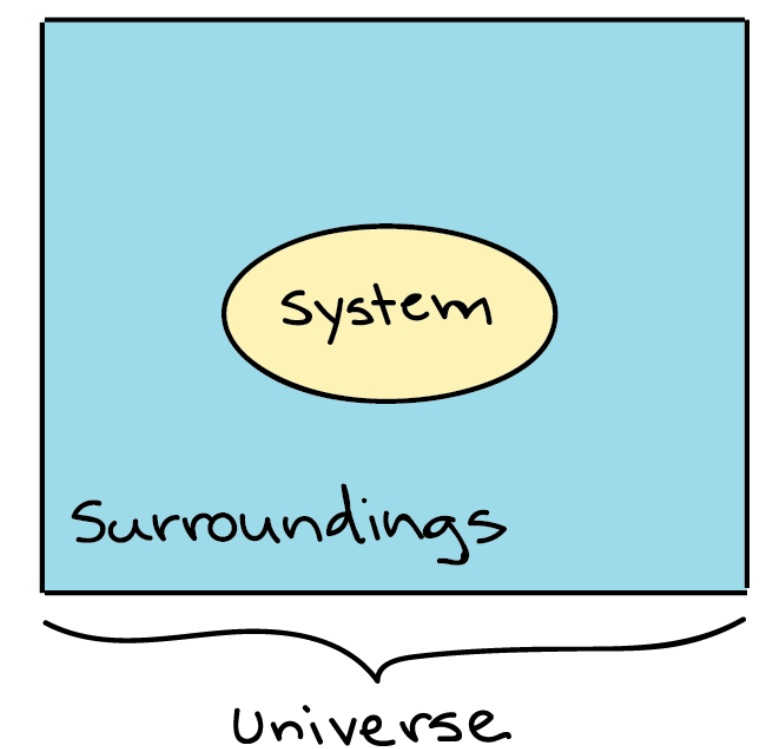
\includegraphics[width=0.4\textwidth]{figures/syst}
	\caption{The definition of a system and its surroundings in thermodynamics.}
	\label{fig:syst}
\end{figure}
The system and the surroundings together make up the universe. In general there are three categorizations of systems in thermodynamics:
\begin{enumerate}
	\item \emph{Open:} An open system is defined as a system that can exchange both energy and matter with its surroundings.
	
	\item \emph{Closed:} A closed system can exchange neither energy nor matter with its surroundings.
	
	\item \emph{Isolated:} An isolated system  can exchange either energy or matter with its surroundings.
\end{enumerate}
The system is said to be in thermodynamic equilibrium if the macroscopic variables characterizing the system (eg. $T,P,V,\dots$ of a gas) is independent of time. Central to thermodynamics is the notion of functions of state, the four laws to thermodynamics and the analysis of system stability.

\section{Functions of state}
As mentioned, a system is in thermodynamic equilibrium if the macroscopic observables are independent of time. The macroscopic observables are functions of state. A function of state is defined as the negative gradient of some abstract, conservative vector field(just like the case of equation \eqref{w6}). That is, a function of state is defined from the path integral
\begin{equation}
	\int_{\vec{x}_i}^{\vec{x}_f}df=f(\vec{x}_f)-f(\vec{x}_i).
	\label{f2}
\end{equation} 
The force field corresponding to the potential function is usually not ascribed any physical interpretation, it is the potential that has physical significance in this case - Since the potential is the physical observable. In general the differential of a function of state is called an exact differential. 
\begin{example}
	A conservative vector field has many useful properties, one of which is that the curl of the vector field is 0. This translates to symmetry of the second derivatives of the potential function. Eg. for a potential $U=U(S,V)$
	\begin{equation}
		\frac{\partial^2U}{\partial S\partial V}=\frac{\partial ^2U}{\partial V\partial S},
	\end{equation} 
	where $S,V$ at this point can be considered as nothing more than variables. Later on they can be considered as entropy($S$) and volume($V$). In thermodynamics, such relations are called Maxwell relations and will prove very useful when the potentials are expressed in terms of state functions.
\end{example}

\section{The laws of thermodynamics}
There are three principal laws of thermodynamics, however, these are supplemented by what is called the zeroth law of thermodynamics to make up four laws in total. Each law leads to the definition of thermodynamic properties which enables one to understand and predict the operation of a physical system.

\begin{enumerate}
	\item \emph{The zeroth law:} The zeroth law of thermodynamics state that two systems, each separately in thermal equilibrium with a third, are in equilibrium with each other. 
	
	\item \emph{The first law:} The first law of thermodynamics state that energy is conserved and heat and work are both forms of energy. The energy under consideration in thermodynamics is the internal energy, $U$. The internal energy is the sum of all the energy of all the internal degrees of freedom that the system posses. It is a function of state since the energy of a system is independent of how the energy is acquired. The internal energy of a system can be changed by doing work on the system or by being heated. The heat, $Q$, and work, $W$, are not functions of state since they describe how energy is delivered to the system. The equation describing the differential change in internal energy is the equation associated to the first law of thermodynamics
	\begin{equation}
		dU=\dbar Q+\dbar W,
	\end{equation} 
	where the bar-notation denotes inexact differentials. $\dbar Q>0$ is the heat applied to the system and $\dbar W>0$ is the work done on the system. $\dbar Q>0$.
	
	\item \emph{The second law:} The second law of thermodynamics can be formulated as a statement about the direction of heat flow that occurs as the system approaches equilibrium from an out of equilibrium state; no process is possible whose sole result is the transfer of heat from a colder to a hotter body. The most common manifestation of the second law of thermodynamics is in terms of entropy. Entropy in again defined in terms of the heat change under a reversible process. A reversible process is a process in which the system and surroundings can be restored to the initial state from the final state without producing any changes in the thermodynamic variables of the universe. In practice most processes are reversible\footnote{The macroscopic variables(eg. T, V,P) are only defined in equilibrium, so a quasi-static process has the macroscopic variables defined all the time - Unlike a process which is not quasi-static by fast.} if they are made sufficiently slow (quasi-static) such that the system passes through a series of equilibrium states between two macro-states. Any reversible process is quasi-static, but not all quasi-static processes are reversible. For example, a quasi-static process involving friction in the mechanics will not be reversible. In general are processes which involve a heat transfer between two systems not reversible. The change of entropy ($dS$) is defined in terms of the reversible change of heat $\dbar Q_{rev}$ as follows
	\begin{equation}
		dS=\frac{\dbar Q_{rev}}{T}.
	\end{equation} 
	The entropy is a state function so the differential is exact. Therefore, taking the endpoint to equal the initial point
	\begin{equation}
		\oint dS=\oint \frac{\dbar Q_{rev}}{T}=0.
		\label{ss1}
	\end{equation} 
	From Clausius theorem, for a process containing irreversible parts~\citep{blundell}
	\begin{equation}
		\oint \frac{\dbar Q}{T}\leq 0.
		\label{q1}
	\end{equation} 
	Taking $a\Rightarrow b$ to be done irreversibly and $b\Rightarrow a$ to be done reversible
	\begin{equation}
		\int_{a}^{b}\frac{\dbar Q}{T}+\int_{b}^{a}\frac{\dbar Q_{rev}}{T}\leq 0\Rightarrow \int_a^b\frac{\dbar Q}{T}\leq \int_{a}^{b}\frac{\dbar Q_{rev}}{T}.
		\label{q2}
	\end{equation} 
	Equation \eqref{q2} holds true however close $a,b$ are as points in state space. So, in general
	\begin{equation}
		dS=\frac{\dbar Q_{rev}}{T}\geq \frac{dQ}{T}.
		\label{q3}
	\end{equation} 
	The equality in $\geq$ only holds if the process is reversible. For an isolated system $\dbar Q=0$, so in general
	\begin{equation}
		dS\geq 0.
		\label{q4}
	\end{equation} 
	Equation \eqref{q4} states that any change for a thermally isolated system results in the entropy staying the same (for a reversible process) or increasing (for an irreversible process). This leads to another statement of the second law of thermodynamics; the entropy of an isolated system tends to a maximum. Equation \eqref{q4} is the manifestation of this version of the second law and is often used in analyzing the stability of thermodynamic systems. This version of the second law is also often applied to the universe. Taking th entire universe to be a closed system, it is clear that the entropy of the universe can only stay the same or go up\footnote{This description is on average. In analyzing the movement of individual molecules the entropy can indeed be found to go down.}. Taking $\dbar Q_{rev}=TdS$ and $\dbar W=-pdV+\mu dN+\dots$, where $p$ is pressure, $V$ is volume, $\mu$ is chemical potential and $N$ is the number of particles, the first law can be written viz
	\begin{equation}
		dU=TdS-pdV+\mu dN+\dots|_{rev}.
		\label{q5}
	\end{equation} 
	Equation \eqref{q5} is valid for reversible processes only at first glance. However, since all quantities in equation \eqref{q5} are functions of state (exact differentials), and therefore independent of the path in state space, the equation holds for irreversible processes as well. In irreversible processes $\dbar Q<0$ and $\dbar W>0$ such that $dU$ is the same whether the change is reversible or not. Hence, in general
	\begin{equation}
		dU=TdS-pdV+\mu dN+\dots.
		\label{q6}
	\end{equation} 
	
	\item \emph{The third law:} The third law of thermodynamics state that the entropy of all systems in internal equilibrium is the same at $T=0K$ (at absolute zero Kelvin), and may be taken to be zero, i.e.; $S(T=0K)=0$.
	
\end{enumerate} 

\section{Manipulation of thermodynamic potentials}	
A central part of practical application of thermodynamics is consist of manipulation of the thermodynamic potentials at hand. From the first law of thermodynamics
\begin{equation}
	dU=TdS-pdV+\mu dN+\dots.
	\label{qq1}
\end{equation} 
Note that $U=U(S,V,N,\dots)$. The potential $U$ can be transformed to another potential function, which is a function of different state functions, by performing a Legendre transformation(just as in advanced classical mechanics). The potential $U=U(S,V,N,\dots)$ can be transformed to the potential $F(T,V,N,\dots)$ viz
\begin{equation}
	\begin{split}
		dU&=TdS-pdV+\mu dN\dots\\
		&=d(TS)-SdT-pdV+\mu dN\dots.\\
	\end{split}
	\label{q12}
\end{equation} 
Taking $d(TS)$ to the left hand side of equation \eqref{q12} reveals
\begin{equation}
	\begin{split}
		dF(T,V,N,\dots)&=d(U(S,V,N,\dots)-TS)\\
		&=-SdT-pdV+\mu dN\dots.
	\end{split}
\end{equation} 
From the thermodynamic potentials, the equations of state are defied as the partial derivatives. From equation \eqref{q12}
\begin{equation}
	T=\frac{\partial U}{\partial S}\bigg|_{V,N,\dots}, \quad -p=\frac{\partial U}{\partial V}\bigg|_{S,N,\dots}, \quad \mu=\frac{\partial U}{\partial N}\bigg|_{S,V,\dots}, \quad \dots.
	\label{q7}
\end{equation} 
Similar equations of state can be derived from $F$. The equation of equation \eqref{q7} are called equations of state. Equations of state are the first partial derivatives of thermodynamic potentials. Now, from the Maxwell relations
\begin{equation}
	\begin{split}
		&\frac{\partial^2 U}{\partial S\partial V}=\frac{\partial^2 U}{\partial V\partial S}\Rightarrow -\frac{\partial p}{\partial S}\bigg|_{_{N,\dots}}=\frac{\partial T}{\partial V}\bigg|_{_{N,\dots}},\\
		&\frac{\partial^2 U}{\partial N\partial V}=\frac{\partial^2 U}{\partial V\partial N}\Rightarrow -\frac{\partial p}{\partial N}\bigg|_{_{S,\dots}}=\frac{\partial \mu}{\partial V}\bigg|_{_{S,\dots}},\\
		&\frac{\partial^2 U}{\partial N\partial S}=\frac{\partial^2 U}{\partial S\partial N}\Rightarrow \frac{\partial T}{\partial N}\bigg|_{_{V,\dots}}=\frac{\partial \mu}{\partial S}\bigg|_{_{V,\dots}}.\\
	\end{split}
	\label{q8}
\end{equation} 
The Maxwell relations are often supplemented by mathematical tools such as Eulers triangle rule and the reciprocal theorem. Eulers triangle rule
\begin{equation}
	\text{Eulers triangle rule:} \quad \frac{\partial S}{\partial T}\bigg|_{_{V,N,\dots}}\frac{\partial T}{\partial V}\bigg|_{_{S,N,\dots}}\frac{\partial V}{\partial S}\bigg|_{_{T,N,\dots}}=-1.
	\label{q9}
\end{equation} 
Note how the derivatives are cyclic, and the relation can be composed from just \textbf{one} partial derivative. The reciprocal theorem
\begin{equation}
	\text{Reciprocal tehorem:}\quad \Rightarrow \frac{\partial S}{\partial V}\bigg|_{_{T,N,\dots}}=\frac{1}{\frac{\partial V}{\partial S}\big|_{_{T,N,\dots}}}.
	\label{q10}    
\end{equation} 

\begin{example}
	Eulers triangle rule and the reciprocal theorem are often used in conjunction to rewrite state functions viz
	\begin{equation}
		\frac{\partial S}{\partial T}\bigg|_{_{V,N,\dots}}=-\frac{\partial S}{\partial V}\bigg|_{_{T,N,\dots}}\frac{\partial V}{\partial T}\bigg|_{_{S,N,\dots}}  .
	\end{equation}  
	In this way, a possibly non-calculable differential can be turned into a perhaps calculate-able one. These relations can in turn be combined with the equations of state and the Maxwell relations in order to really make the magic happen. 
\end{example}

\section{System stability}
In thermodynamics the thermodynamic potentials are often used to analyze the stability of the system. The condition for stability is that for fixed variables, any change in the thermodynamic potential system must be positive. For example for $F=F(T,V,N)$ when $T,V,N$ are fixed, $\delta F \geq0$. Another way of stating this is that if you leave a system alone, it is stable if it is in a minimum of the potential. In the minimum, every change in the potential is positive! In equilibrium, the potential must be convex. A convex function has a positive curvature. This is mathematically expressed as
\begin{equation}
	d^2F>0
\end{equation}   
To examine the stability, investigate the fluctuations between two subsystems, when the system is in a stable equilibrium. Take $N=const$, while allowing $T,V$ to vary. A small perturbation in the potential can then be written as follows
\begin{equation}
	\delta F=F_2(T+\Delta T, V+\Delta V, N)+F_1(T-\Delta T, V- \Delta V, N) - 2F(T,M,N)\geq 0,
	\label{variationF}
\end{equation} 
where the last term is included to subtract the average offset of the potential. Only the fluctuations around the minimum is of interest, not with respect to the arbitrary reference value that has been chosen. Next, Taylor expand $F_1 $ and $F_2$
\begin{equation}
	\begin{split}
		&F_2=F(T,V,N)+\frac{\partial F}{\partial T}\bigg|_{_{V,N}}\Delta T+\frac{\partial F}{\partial V}\bigg|_{_{T,N}}\Delta V\\
		&\qquad+\frac{1}{2}\bigg(\frac{\partial^2 F}{\partial T^2}\bigg|_{_{V,N}}(\Delta T)^2+\frac{\partial^2 F}{\partial V^2}\bigg|_{_{T,N}}(\Delta V)^2+2\frac{\partial^2 F}{\partial T \partial V}\bigg|_{_{N}}\Delta M \Delta T \bigg)+...,\\
		&F_1=F(T,V,N)-\frac{\partial F}{\partial T}\bigg|_{_{V,N}}\Delta T-\frac{\partial F}{\partial V}\bigg|_{_{T,N}}\Delta V\\
		&\qquad+\frac{1}{2}\bigg(\frac{\partial^2 F}{\partial T^2}\bigg|_{_{V,N}}(\Delta T)^2 +\frac{\partial^2 F}{\partial V^2}\bigg|_{_{T,N}}(\Delta V)^2+2\frac{\partial^2 F}{\partial T \partial V}\bigg|_{_{N}}\Delta V \Delta T \bigg)+...,
	\end{split}
	\label{taylor}
\end{equation}  
where the terms of higher order is neglected in the usual analysis of stability. By inserting equation \eqref{taylor} in equation \eqref{variationF}, the first order terms, along with the zero order terms, disappear and leave only the second order terms. Let the changes go to infinitesimal sizes ($\Delta \Rightarrow d$) to find
\begin{equation}
	\delta F\cong\frac{\partial^2 F}{\partial T^2}\bigg|_{_{V,N}}(dT)^2+\frac{\partial^2 F}{\partial V^2}\bigg|_{_{T,N}}(dV)^2+2\frac{\partial^2 F}{\partial T \partial V}\bigg|_{_{N}}dVdT=d^2F > 0.
	\label{d^2F}
\end{equation} 
The "$\cong$" in equation \eqref{d^2F} come from neglecting higher order terms from the Taylor series. Equation \eqref{d^2F} can be written in matrix form
\begin{equation}
	d^2F=
	\begin{bmatrix}
		dT & dV\\
	\end{bmatrix}
	\begin{bmatrix}
		\frac{\partial^2 F}{\partial T^2}\bigg|_{_{V,N}}       & \frac{\partial^2 F}{\partial T \partial V}\bigg|_{_{N}}  \\
		\frac{\partial^2 F}{\partial T \partial V}\bigg|_{_{N}}       &
		\frac{\partial^2 F}{\partial V^2}\bigg|_{_{T,N}}
		\\
	\end{bmatrix}
	\begin{bmatrix}
		dT\\
		dV\\
	\end{bmatrix} > 0.
	\label{matrix1}
\end{equation} 
Since the matrix is symmetric, it can be diagonalized with the eigenvalues in the diagonal. That is, equation \eqref{matrix1} can be written on the form
\begin{equation}
	d^2F=
	\begin{bmatrix}
		dT & dV\\
	\end{bmatrix}
	\begin{bmatrix}
		\lambda_1       & 0  \\
		0       &
		\lambda_2
		\\
	\end{bmatrix}
	\begin{bmatrix}
		dT\\
		dM\\
	\end{bmatrix}=\lambda_1(dT)^2+\lambda_2(dV)^2 > 0.
\end{equation} 
For this expression to hold for every possible eigenvalue, the eigenvalues must be positive. Since they must be positive, the determinant and trace of the diagonalized matrix must be positive as well. That is
\begin{equation}
	\begin{split}
		det
		\begin{bmatrix}
			\lambda_1       & 0  \\
			0       &
			\lambda_2
			\\
		\end{bmatrix}&=\lambda_1 \lambda_2 >0,\\
		tr
		\begin{bmatrix}
			\lambda_1       & 0  \\
			0       &
			\lambda_2
			\\
		\end{bmatrix}&=\lambda_1 + \lambda_2 >0.
	\end{split}
\end{equation} 
Note that the determinant can be positive if both eigenvalues are negative, and the trace can be positive if the smallest eigenvalue is negative. If both conditions are fulfilled, then both eigenvalues must be positive. A diagonalization is a linear transformation. Under such a transformation both the determinant and trace are conserved quantities. That means the trace and determinant of the diagonalized matrix can be determined directly from the undiagonalized matrix. No diagonalization have to be performed in practice. The determinant and trace of the "middle" matrix in equation \ref{matrix1}, are in this case found to be:
\begin{equation}
	\begin{split}
		det
		\begin{bmatrix}
			\frac{\partial^2 F}{\partial T^2}\bigg|_{_{V,N}}       & \frac{\partial^2 F}{\partial T \partial V}\bigg|_{_{N}}  \\
			\frac{\partial^2 F}{\partial T \partial V}\bigg|_{_{N}}       &
			\frac{\partial^2 F}{\partial V^2}\bigg|_{_{T,N}}
			\\
		\end{bmatrix}
		&=\frac{\partial^2 F}{\partial T^2}\bigg|_{_{V,N}}\frac{\partial^2 F}{\partial V^2}\bigg|_{_{T,N}}-\bigg(\frac{\partial^2 F}{\partial T \partial V}\bigg|_{_{N}}\bigg)^2 >0\\
		tr
		\begin{bmatrix}
			\frac{\partial^2 F}{\partial T^2}\bigg|_{_{V,N}}       & \frac{\partial^2 F}{\partial T \partial V}\bigg|_{_{N}}  \\
			\frac{\partial^2 F}{\partial T \partial V}\bigg|_{_{N}}       &
			\frac{\partial^2 F}{\partial V^2}\bigg|_{_{T,N}}
			\\
		\end{bmatrix}
		&=\frac{\partial^2 F}{\partial T^2}\bigg|_{_{V,N}}+\frac{\partial^2 F}{\partial V^2}\bigg|_{_{T,N}}>0
	\end{split}
	\label{det}
\end{equation} 
After this expression is reached, the expressions for the derivatives must be analyzed in order to interpret the physical content of the stability of the system \footnote{Note that \ref{det} is derived on the basis that a perturbation in V and T is performed whilst N is held constant. If these conditions are not met, the equations does not hold(!).}. The second derivatives couple to the heat capacities, so the stability of the system couples to the allowed signs of the heat capacities\footnote{Often they must be positive in a stable system}. Further more, the general derivatives can be analyzed by determining whether a thermodynamic variable is extensive or intensive. Thermodynamic potentials are convex functions of their extensive variables, and concave functions of their intensive variables. For example the temperature is an intensive variable; it does not change if the system size is altered. From this it can be concluded that $\frac{\partial^2 F}{\partial T^2}\big|_{_{M,N}}\leq0$. Likewise for other thermodynamic variables and potentials\footnote{That goes for the evaluation of the second derivatives as well as the stability treatment of the potential.}.
	
	\part{Quantum Mechanics}
		\chapter{Mathematical setup}
Quantum mechanics is the science of small systems in which the particles move at non-relativistic speeds. The involved speeds need to be non-relativistic (i.e. relatively low) since if the this is not the case, the energies involved will be so large that particles can be created and annihilated. Since conservation of particle number is central in QM it cannot accommodate a variable number of particles without problems. This is the reason for introducing QFT later on. \newline
A quantum mechanical system is defined as a system which is disturbed by the act of (a very careful) measurement\footnote{There exist several interpretations of quantum mechanics, including The Copenhagen interpretation and Bohmian mechanics (pilot wave theory). The former assume probability waves are the true nature of quantum mechanics and upon measurement the probability wave collapse into a particle. The latter assume there is a real particle that are pused around by real waves of unknown nature. The two interpretations yield the same predictions, but have different interpretations. Only the Copenhagen interpretation, however, have a relativistic version in QFT. This is because QFT require all possible particle paths to be equally real, which is not the case in Bohmian mechanics where there is a real particle that takes a single path.}. In the words of Paul Dirac~\citep{dirac}
\begin{quote}
	“\textit{... We have to assume that there is a limit to the finiteness of our powers of observation and the smallness of the accompanying disturbance - a limit which is inherent in the nature of things and can never be surpassed by improved technique or increased skill on the part of the observer.}”
\end{quote}
Because measurements disturb the systems in quantum mechanics the QM system is fundamentally different from a system of classical mechanics. In classical mechanics the physical state of a system can be specified by specifying the system particles' positions and momenta ($q_i,p_i$) at a given time. Because the act of measurement disturbs a quantum mechanical system, the data that can be assigned to a quantum mechanical system depends on whether or not measurements of the different quantities disturb each other. In the words of Paul Dirac~\citep[p.11]{dirac}
\begin{quote}
	“\textit{The limitation in the power of observation puts a limitation on the number of data that can be assigned to a state. Thus a state of an atomic system must be specified by fewer or more indeterminate data...}”
\end{quote} 
\begin{quote}
	“\textit{A state of a system may be defined as an undisturbed motion that is restricted by as many conditions or data as are theoretically possible without mutual interference or contradiction.}”
\end{quote} 

\section{The vector space of quantum mechanics}
Because of this difference (from classical mechanics) the quantum mechanical state of a system is represented as a vector, called the \emph{state vector}\index{State vector}, in a complex vector space of $N$ dimensions. If the possible results of a measurement make up an infinite set, as is the case when measuring position or momentum, the vector space is of infinite dimension and called a \emph{Hilbert space}\index{Hilbert space}\footnote{However, physicists often denote the vector space of quantum mechanics a Hilbert space even if the dimensions are finite!}. I shall use the notation of Paul Dirac, and call a vector in the complex vector space (of any dimension) a \emph{ket}. I will refer to general vectors representing a general physical state as $\ket{\alpha},\ket{\beta}, \ket{\gamma},...$. Initially I will take the state vector to the independent of time. This provides the opportunity to introduce symmetry operators and derive the Schroedinger equation later on\footnote{How to describe the time-dependence of the state vector is, as so many other things in QM, a matter of taste.}. For two arbitrary vectors, $\ket{\alpha}$ and $\ket{\beta}$, in the complex vector space the following axioms ~apply\citep{Sakurai}.
\begin{enumerate} 
	\item Two vectors can be added to form a new vector
	\begin{equation}
		\ket{\alpha}+\ket{\beta}=\ket{\gamma}.
	\end{equation}  
	\item Vector addition is cumulative
	\begin{equation}
		\ket{\alpha}+\ket{\beta}=\ket{\beta}+\ket{\alpha}.
	\end{equation} 
	\item Vector addition is associative
	\begin{equation}
		(\ket{\alpha}+\ket{\beta})+\ket{\gamma}=\ket{\beta}+(\ket{\alpha}+\ket{\gamma}).
	\end{equation} 
	\item There is a unique vector which can be added, to another vector, which results in the first vector(null vector)
	\begin{equation}
		\ket{0}+\ket{\alpha}=\ket{\alpha}.
	\end{equation} 
	\item Given any ket, there is a unique ket that when added results in zero
	\begin{equation}
		\ket{\alpha}+(-\ket{\alpha})=0.
	\end{equation} 
	\item The distributive property holds (for a complex number $c$)
	\begin{equation}
		c(\ket{\alpha}+\ket{\beta})=c\ket{\alpha}+c\ket{\beta}.
	\end{equation} 
	\item Vectors can be multiplied with a complex number to form a new vector
	\begin{equation}
		c\ket{\alpha}=\ket{\alpha'}.
	\end{equation} 
\end{enumerate}
Axioms 6 and 7 together are called linearity. Ordinary 3-vectors would satisfy these axioms, except for one thing: Axiom 7 allows a vector to be multiplied with a complex number, whereas ordinary 3-vectors are only allowed to be multiplied with a real number. If axiom 7 is applied to the state vector, it would change the length of the vector, but not the physical state the vector is referring to - it is only the direction, not the magnitude, of the state vector that is of importance (regarding the physical state of the system).\newline
Just like complex numbers have dual versions in the form of complex conjugate numbers, so have the ket vector space a dual version that is essentially the complex conjugate version. This dual vector space contains vectors called bra's. For each ket there exists a bra and there is a one-to-one correspondence between the vectors in the two vector spaces, i.e. for each ket $\ket{\alpha}$ there exists a bra $\bra{\alpha}$. The above axioms containing kets apply for bra's if all kets are replaced with bra's.\newline
Because the act of measurement disturbs the system, measurements in quantum mechanics are represented by operators, which are applied to the state vector. Operators representing a measurable physical quantity are called \emph{observables}, and could be position ($x, y,z$), momentum($p$), energy($H$) and so on\footnote{A common notation for operators is a hat. However, this notation is absent in more advanced texts and so it is a good exercise to get used to it from the beginning.}. Mathematically a general operator, $A$, operates on the ket to its right to form a new ket
\begin{equation}
	A\cdot(\ket{\alpha})=A\ket{\alpha}=\ket{\alpha'},
	\label{random}
\end{equation} 
where $\ket{\alpha'}$ just denotes that the result of an operator operating on a ket is just another ket. Likewise, an operator operates on a bra from the right side to form a new bra
\begin{equation}
	(\bra{\alpha})\cdot A=\bra{\alpha}A=\bra{\alpha
		'}.
\end{equation} 
The ket $A\ket{\alpha}$ and bra $\bra{\alpha}A$ are, in general, not dual to each other. The operator operating on a dual bra to create a bra dual to $A\ket{\alpha}$ is denoted as the \emph{Hermitian adjoint of operator}\index{Hermitian adjoint} of an operator. It is defined as
\begin{equation}
	A\ket{\alpha}\iff\bra{\alpha}A^\dagger
\end{equation} 
With the Hermitian adjoint operator comes the following axioms.
\begin{enumerate} 
	\item The Hermitian adjoint of a ket is a bra
	\begin{equation}
		(\ket{\alpha})^\dagger=\bra{\alpha}.
	\end{equation} 
	\item Considering an operator sandwiched by a ket and bra the operator will initially act on the ket to the right, however by taking the Hermitian adjoint of the operator the operator can be made to act on the bra to the right. That is\footnote{The Hermitian adjoint is defined as the operator giving the complex conjugate eigenvalue if operating on a dual eigenvector to the left. If one made the operator operate to the right the outcome would in general not be the complex conjugate eigenvector. So $A^\dagger\ket{a'}\neq a'^*\ket{a'}$.}
	\begin{equation}
		\bra{\beta}(A\ket{a})=(\bra{\beta}A^\dagger)\ket{a}.
	\end{equation} 
	\item The Hermitian adjoint of an operator that is already the Hermitian adjoint of an operator is the operator itself
	\begin{equation}
		(A^\dagger)^\dagger=A.
	\end{equation} 
	\item The Hermitian adjoint is distributive in the way that
	\begin{equation}
		(AB)^\dagger=B^\dagger A^\dagger,
	\end{equation} 
	where  $B$ is just another operator.
	\item The Hermitian adjoint is also distributive in the way that
	\begin{equation}
		(A+B)^\dagger=A^\dagger+B^\dagger.
	\end{equation} 
	\item The Hermitian adjoint of a number is the complex conjugate of the number
	\begin{equation}
		c^\dagger=c^*.
	\end{equation} 
	\item Taking the Hermitian adjoint of two operators reverses the direction they act but also the order
	\begin{equation}
		\bra{\beta}AB\ket{\alpha}=(\bra{\beta}A^\dagger)B\ket{\alpha}=((\bra{\beta}A^\dagger)B^\dagger)\ket{\alpha}.
	\end{equation} 
\end{enumerate}
If an operator is equal to the Hermitian adjoint of itself it is said to be \emph{Hermitian}\index{Hermitian operator}. That is an operator is Hermitian if
\begin{equation}
	A=A^\dagger.
\end{equation} 
This is the case for all operators corresponding to a measurable physical quantity, i.e. for observables. The reason for this is that Hermitian operators have real eigenvalues, and the eigenvalues are the possible outcomes of a measurement\index{Outcome of an experiment, QM}. Since a measurement must be a real number, the operators corresponding to something measurable must be Hermitian. For general operators, $A, B$ and $C$, the following axioms apply.
\begin{enumerate} 
	\item Addition of operators are commutative
	\begin{equation}
		A+B=B+A.
	\end{equation}  
	\item Addition of operators are associative
	\begin{equation}
		A+(B+C)=(A+B)+C.
	\end{equation} 
	\item The majority of operators are linear\footnote{With the exception of the time-reversal operator, all operators in is linear.}
	\begin{equation}
		A(c_\alpha\ket{\alpha}+c_\beta\ket{\beta})=c_\alpha A\ket{\alpha}+c_\beta A\ket{\beta}.
	\end{equation} 
	\item Multiplication of operators are in general \emph{not} commutative
	\begin{equation}
		AB\neq BA.
	\end{equation} 
	\item Multiplication of operators are associative
	\begin{equation}
		A(BC)=(AB)C=ABC.
	\end{equation} 
\end{enumerate}
In general when a linear operator acts on a vector, it will change the direction of the vector. However, for a given operator, there will be a set of vectors that will have the same direction, but possibly a different magnitude, after the operator acts upon them - these vectors are called \emph{eigenvectors}\index{Eigenvector}, and the constant representing the possible change in length of the eigenvector is called the \emph{eigenvalue}\index{Eigenvalue}. It is said that the eigenvectors corresponds to an eigenvalue, and therefore these vectors are written in a special way
\begin{equation}
	A\ket{a'}=a'\ket{a'} \qquad \mbox{and} \qquad \bra{a'}A^\dagger=\bra{a'}a'^*,
	\label{eig1}
\end{equation} 
where the primed notation denote that there can be more, and that the vector and constant belong together in sets. In general when considering a ket that is an eigenvector of some observable I will indicate it with a label (subscript, superscript or primed notation). The eigenvalue is in general a complex number, but for the physically measurable quantities (hermitian operators) the eigenvalues are, as mentioned, what can be the outcome of an experiment, and must be \emph{real}.\newline
With both kets, bras and operators defined, I move on to the inner product. Between the two vector spaces, the ket and bra space, an inner product, which results is a complex number in general, is defined as $\braket{\alpha|\beta}$\footnote{The definition of the inner product is the reason for the names of the ket and bra. When put together to an inner product they form a bracket.}. For the inner product applies the following axioms.
\begin{enumerate} 
	\item Inner products are linear
	\begin{equation}
		\bra{\gamma}(\ket{\alpha}+\ket{\beta})=\braket{\gamma|\alpha}+\braket{\gamma|\beta}.
	\end{equation}  
	\item Interchanging bras and kets correspond to complex conjugation
	\begin{equation}
		\braket{\alpha|\beta}=\braket{\beta|\alpha}^*.
	\end{equation} 
	\item The inner product between corresponding bras and kets is a real, positive number
	\begin{equation}
		\braket{\alpha|\alpha}=\Re\geq 0.
	\end{equation} 
\end{enumerate}
where the equality in axiom 3 only holds if $\ket{\alpha}$ is a null ket and the part about $\braket{\alpha|\alpha}$ being real in axiom 3 follows from axiom 2. Two kets are said to be orthogonal if the inner product between the one as a ket and the other as a bra is zero,  i.e.
\begin{equation}
	\braket{\alpha|\beta}=0.
\end{equation}   
This analog to 3-space, where the inner product between orthogonal vectors, eg. representing two of the axis of 3-space, is zero.  From the inner product a normalized ket can be constructed
\begin{equation}
	\ket{\tilde{\alpha}}=\bigg(\frac{1}{\sqrt{\braket{\alpha|\alpha}}}\bigg)\ket{\alpha}.
	\label{norm}
\end{equation} 
The normalized ket has the property
\begin{equation}
	\braket{\tilde{\alpha}|\tilde{\alpha}}=1.
\end{equation} 
Because $\ket{\alpha}$ and $c\ket{\alpha}$ represent the same physical state, physical states are by convention required to be normalized\footnote{Although obviously an un-normalized state vector corresponds to the same physical.}. In practice when evaluating the inner product the identity operator is used to project the state vector onto a set of basis vectors. The identity operator is defined from the completeness relation (defined in equation \eqref{identity operator} and \eqref{identity operator2}), and state that the sum of outer products (eg. $\ket{a'}\bra{a'}$) between kets of a complete, orthogonal set is $1$. The completeness relation\index{Completeness relation} exists both in a discrete and continuous version
\begin{equation}
	\sum_{a'}^{}\ket{a'}\bra{a'}=1,
	\label{identity operator}
\end{equation}  
\begin{equation}
	\int_{-\infty}^{\infty}\ket{x}\bra{x}dx=1,
	\label{identity operator2}
\end{equation} 
where $a'$ is just an example, and it could be another complete, orthogonal, discrete set of vectors as well (eg. $\ket{n}$) and $1$ is the identity operator; it has the property of  $1\ket{\alpha}=\ket{\alpha}$ for any $\ket{\alpha}$. Equation \eqref{identity operator2} can be used to write the inner product\footnote{Between to identical state vectors in this case - it could be two arbitrary kets in general.} as
\begin{equation}
	\braket{\alpha|\alpha}=\int_{-\infty}^{\infty}\braket{\alpha|x}\braket{x|\alpha}dx,
\end{equation} 
where $\braket{x|\alpha}$ is a complex function called the wave function\footnote{If the variables are defined, the inner product becomes a complex number in general. You can view it as $\braket{x=1|\alpha}=number$ or $\psi(x=1)=number$ - the two are equivalent.}. The wave function is a central element in QM since it describes the state vector in the often utilized position basis. One finds a complete orthogonal set of kets as the eigenkets of \emph{any} arbitrary observable! It is a fundamental theorem of quantum mechanics that the eigenvectors of Hermitian operators make up a complete, orthogonal ($\braket{\alpha|\beta}=\delta_{\alpha\beta}$) set. The complete, orthogonal set of vectors span the vector space in which the operator is defined. Hence, as an example, the complete set from the spin operator span a different vector space than the complete set from the Hamiltonian operator for the harmonic oscillator. This might seem like a mathematical subtlety, however it becomes relevant when the complete, orthogonal set is used to expand a state vector upon.

\section{Matrix notation}
So far I have used the notation of Paul Dirac for the vectors in the complex vector space. However, as is clear from the axioms regarding both operators and kets, the operators and kets obey axioms that are similar to that of linear algebra. This means that operators\footnote{Any \emph{linear} operator can be represented by a matrix. Almost all operators are linear, but not all!}, with discrete eigenvalues, obeying the axioms can be regarded as matrices and kets and bras as vectors. In the words of Paul Dirac~\citep[p.69]{dirac}
\begin{quote}
	“\textit{We can summarize our results for the case when there is only one $\xi$ and it has discrete eigenvalues as follows \newline
		(i) Any linear operator is represented by a matrix. \newline
		(ii) The unit operator is represented by the unit matrix. \newline
		(iii) A real linear operator is represented by a Hermitian matrix.\newline
		(iv) $\xi$ and functions of $\xi$ are represented by diagonal matrices.\newline
		(v) The matrix representing the product of two linear operators is the product of the matrices representing the two factors.}”
\end{quote}

In order to develop the matrix notation I consider the operator $B$. I use the completeness relation twice, such that
\begin{equation}
	B=\sum_{a'}^{}\sum_{a''}^{}\ket{a''}\bra{a''}B\ket{a'}\bra{a'},
	\label{matrixop}
\end{equation} 
where $\{\ket{a'}\}$ is a complete orthogonal set, which are in general \emph{not} eigenvectors of $B$, and $\ket{a''}$ and $\ket{a'}$ are just kets from $\{\ket{a'}\}$. The elements (numbers) $\bra{a''}B\ket{a'}$ determine the operator ($B$) completely. They can be arranged in a matrix to represent $B$ in matrix representation. They are in general calculated by using the completeness relation twice
\begin{equation}
	\begin{split}
		\braket{a''|B|a'}&=\int_{-\infty}^{\infty}\int_{-\infty}^{\infty}\braket{a''|x'}\braket{x'|B|x}\braket{x|a'}dxdx'\\
		&=\int_{-\infty}^{\infty}\psi_{a'}^*(x)b(x)\psi_{a'}(x)dx,
	\end{split}
	\label{B}
\end{equation} 
where\footnote{$\psi_{a'}(x)$ is completely analog to $\psi_n(x)$.} I have used that $B=B(x)$, and thereby the eigenvalues of the operator can be inserted in its place; $B(x)\ket{x}=b(x)\ket{x}$. The eigenvalue of the operator is the "scalar" operator in the position basis. This is analog to the known relation $V(x)\ket{x}=V(x)\ket{x}$. By using $B(x)\ket{x}=b(x)\ket{x}$ I find that $\braket{x'|B|x}=b(x)\delta(x'-x)$ - which reduces the double integral to a single integral. To interpret the physical significance of the the matrix elements, $\braket{i|B|j}$, I cite from \citet[p.45]{dirac}
\begin{quote}
	“\textit{In classical mechanics an observable always, as we say, 'has a value' for any particular state of the system. What is there in quantum mechanics corresponding to this? If we take any observable $\xi$ and any two states $x$ and $y$, corresponding to the vectors $\bra{x}$ and $\ket{y}$, then we can form the number $\braket{x|\xi|y}$. This number is not very closely analogous to the value which an observable can 'have' in the classical theory, for the reasons, namely, (i) it refers to \emph{two} states of the system, while the classical value always refers to \emph{one}, (ii) it is in general not a real number, and (iii) it is not uniquely determined by the observables and the states, since the vectors $\bra{x}$ and $\ket{y}$ contain arbitrary numerical factors. Even if we impose on $\bra{x}$ and $\ket{y}$ the condition that they shall be normalized, there will still be an undetermined factor of modulus unity in $\braket{x|\xi|y}$. These three reasons cease to apply, however, if we take the two states to be identical and $\ket{y}$ to be the conjugate imaginary vector to $\bra{x}$. The number that we then get, namely $\braket{x|\xi|x}$ is necessarily real, and also it is uniquely determined when $\bra{x}$ is normalized, since we multiply $\bra{x}$ by the numerical factor $e^{ic}$, c being some real number, we must multiply $\ket{x}$ by $e^{-ic}$ and $\braket{x|\xi|x}$ will be unaltered.\newline(...) We therefore make the general assumption that if the measurement of the observable $\xi$ for the system in the state corresponding to $\ket{x}$ is made a large number of times, the average of all the results obtained will be $\braket{x|\xi|x}$, provided $\ket{x}$ is normalized. If $\ket{x}$ is not normalized, as is necessarily the case if the state x is an eigenstate of some observable belonging to an eigenvalue in a range, the assumption becomes that the average result of a measurement of $\xi$ is proportional to $\braket{x|\xi|x}$.}”
\end{quote}
To recap; the general element $\braket{i|B|j}$ does not hold any special position whilst $\braket{i|B|i}$ denotes the expectation value of measuring the operator $B$. In matrix notation, and in the basis of $\ket{a'}$, the operator, $B$, can be represented by
\begin{equation}
	B\doteq\begin{bmatrix}
		\braket{a'|B|a'} & \braket{a'|B|a''}&\dots\\
		\braket{a''|B|a'} & \braket{a''|B|a''} &\\
		\vdots&  &\ddots\\
	\end{bmatrix},
	\label{matrix11}
\end{equation}  
where $\ket{a'}$,as states before, in general are not the eigenvectors of $B$. In the special case where the basis kets \emph{are} eigenvectors of the operator, equation \eqref{matrixop} reduces to
\begin{equation}
	A=\sum_{a'}^{}\sum_{a''}^{}\ket{a''}\bra{a''}A\ket{a'}\bra{a'}=\sum_{a'}^{}a'\ket{a'}\bra{a'},
	\label{matrixop1}
\end{equation} 
where I have used that the square matrix $\bra{a''}A\ket{a'}$ is diagonal in its eigenbasis. Therefore
\begin{equation}
	\bra{a''}A\ket{a'}=\bra{a'}A\ket{a'}\delta_{a'a''}=a'\delta_{a'a''}.
	\label{matrixop2}
\end{equation} 
Equation \eqref{matrixop1} is used to express an operator when the eigenvalues and eigenvectors are known.\newline
Going back to the general case where the basis is not the eigenbasis of the operator; I use the information (that $B$ can be represented as a matrix) to define kets and bras as vectors. I use equation \eqref{random} with $B$ instead of $A$, and the general kets $\ket{\gamma}$ and $\ket{\alpha}$ instead of the eigenkets. I write
\begin{equation}
	\ket{\gamma}=B\ket{\alpha}.
\end{equation}  
I now sandwich with $\bra{a'}$ from the left and insert the completeness relation
\begin{equation}
	\braket{a'|\gamma}=\sum_{a''}^{}\bra{a'}B\ket{a''}\braket{a''|\alpha}.
	\label{vector def}
\end{equation}  
Equation \eqref{vector def} can be considered as a linear transformation. The matrix is represented by the elements $\bra{a'}B\ket{a''}$ whereas the kets are represented by the vector elements $\ket{\alpha}\doteq\braket{a''|\alpha}$ and $\ket{\gamma}\doteq\braket{a'|\gamma}$. Thus, I can represent the kets in vector notation as
\begin{equation}
	\ket{\alpha^j}\doteq\begin{bmatrix}\braket{a'|\alpha^j}\\ \braket{a''|\alpha^j}\\ \braket{a'''|\alpha^j}\\ \vdots \\\braket{a^{i}|\alpha^j}\end{bmatrix}, \quad
	\ket{\gamma^j}\doteq\begin{bmatrix}\braket{a'|\gamma^j}\\ \braket{a''|\gamma^j}\\ \braket{a'''|\gamma^j}\\ \vdots \\\braket{a^{i}|\gamma^j}\end{bmatrix},
\end{equation} 
where the superscript "j" denotes that there are different eigenvectors of $B$ - each corresponding to an eigenvalue. As for the bra's; in matrix notation they are represented as the complex conjugate transposed of the kets. Thus, the inner product can be written in matrix form as 
\begin{equation}
	\braket{a|b}=\begin{bmatrix}a_1^* & a_2^* & a_3^* &...& a_i^* \end{bmatrix}\begin{bmatrix}b_1\\ b_2\\ b_3\\ \vdots  \\b_i\end{bmatrix}=a_1^*b_1+\dots a_i^*b_i.
\end{equation} 
So, what is the purpose of going to a matrix notation instead of the notation of Dirac? Well, first of all; most people are more used to linear algebra, so it is more familiar to them, but the main reason is because the eigenvalue problem, given eg. by equation \eqref{eig1}, can be solved quite neatly by using linear algebra. To illustrate this I consider the task of finding the eigenvalues and eigenvectors of an operator, $B$. The eigenvectors and eigenvalues of $B$ are defined from the eigenvalue equation
\begin{equation}
	B\ket{b'}=b'\ket{b'},
	\label{eig2}
\end{equation} 
where $b'$ and $\ket{b'}$ are to be determined. I sandwich equation \eqref{eig2} from the left with $\bra{a''}$, which I assume is from the \emph{known} set $\{\ket{a'}\}$(else I would not be able to calculate the matrix elements), and use the completeness relation\footnote{I take $\ket{a'}$ to (still) be the eigenkets of an observable, and therefore make up a complete set of orthogonal vectors. Thus, i can use the completeness relation.}
\begin{equation}	\sum_{a'}^{}\bra{a''}B\ket{a'}\braket{a'|b'}=b'\braket{a''|b'}.
	\label{matrix5}	
\end{equation} 
Equation \eqref{matrix5} can be written in matrix notation as
\begin{equation}
	\begin{bmatrix}
		\braket{a'|B|a'} & \braket{a'|B|a''}&\dots\\
		\braket{a''|B|a'} & \braket{a''|B|a''} &\\
		\vdots& & \ddots \\
	\end{bmatrix}
	\begin{bmatrix}
		\braket{a'|b'}\\
		\braket{a''|b'}\\
		\vdots\\
	\end{bmatrix}
	=b'\begin{bmatrix}
		\braket{a'|b'}\\
		\braket{a''|b'}\\
		\vdots\\
	\end{bmatrix}.
	\label{matrixeig1}
\end{equation}  
From Cramers rule, equation \eqref{matrixeig1} only has non-trivial for $\braket{a^{(k)}|b^{(l)}}$ when
\begin{equation}
	det(B-\lambda I)=0,
	\label{cramer1}
\end{equation} 
where $I$ is the identity matrix. This corresponds to diagonalizing\footnote{When diagonalization of an operator is mentioned the operator is always implicitly thought of in matrix notation.} $B$. The eigenvalues of $B$ are the eigenvalues of $B$ and the eigenvectors of $B$ make up the coefficients $\braket{a^{(k)}|b^{(l)}}$, which are the elements of the eigenvectors of $B$. Thus
\begin{equation}
	\lambda_i=b^i=\mbox{eigenvalues of $B$},
\end{equation} 
\begin{equation}
	\ket{b'}\doteq\begin{bmatrix}
		\braket{a'|b'}\\
		\braket{a''|b'}\\
		\vdots\\
	\end{bmatrix}= \mbox{the b'th eigenvector of $B$}.
	\label{eigenket}
\end{equation} 
The elements, $\braket{a^{(k)}|b^{(l)}}$, of the eigenvectors, $\ket{b^{(l)}}$, can be arranged into a matrix called the \emph{transformation matrix} ($U$) \index{Transformation matrix}, which can be used to transform an operator, or state vector, from the basis of $\ket{a'}$ to the basis of $\ket{b'}$. I will come back to how the eigenvectors fit into the transformation matrix, but before I do so, let me make a formal introduction of the transformation operator! A transformation of basis becomes relevant when one considers two non-commuting observables. These does not have simultaneous eigenvectors, but since they are both observables, their eigenvectors clearly make a complete, orthogonal set and span the same vector space. Thus, one might be interested in changing from representing a given state vector, say $\ket{\alpha}$, in one basis to the other. To this end the transformation operator is used. To be more explicit, I consider the eigenkets of two non-commuting observables, $A$ and $B$ ($[A,B]\neq0$); $\{\ket{a'}\}$ and $\{\ket{b'}\}$. I define the operator corresponding to the transformation matrix as the operator responsible for a basis transformation
\begin{equation}
	U\ket{a^{(l)}}=\ket{b^{(l)}}.
	\label{eig3}
\end{equation} 
The obvious representation of $U$ is\footnote{Because it operates on $\ket{a^{(l)}}$ with $\bra{a^{(k)}}$. Since there kets are orthogonal the inner product is $1$ when $a^{(l)}=a^{(k)}$ and $0$ otherwise. In the case where it is $1$, the corresponding ket $\ket{b^{(k)}}=\ket{b^{(l)}}$ gets to "survive" - the rest of the b's don't.}
\begin{equation}
	U=\sum_{k}^{}\ket{b^{(k)}}\bra{a^{(k)}}.
	\label{unit}
\end{equation} 
From equation \eqref{unit} it is clear that $U$ is a unitary operator ($UU^\dagger=1$). I can represent $U$ in matrix form by multiplying $\bra{a^{(k)}}$ from the left
\begin{equation}
	\bra{a^{(k)}}U\ket{a^{(l)}}=\braket{a^{(k)}|b^{(l)}}.
	\label{trans matrix}
\end{equation} 
From equation \eqref{trans matrix} it is clear that the elements of the transformation matrix is the elements of the eigenvectors of $B$. In matrix notation
\begin{equation}
	U=
	\begin{bmatrix}
		\braket{a^{1}|b^{1}} & \braket{a^{1}|b^{2}}&\dots\\
		\braket{a^{2}|b^{1}} & \braket{a^{2}|b^{2}} &&&\\
		\vdots& &\ddots \\
	\end{bmatrix}=
	\begin{bmatrix}
		&&&&\\
		&&&&\\
		\ket{b^{1}} & \ket{b^{2}}&\dots\\
		&&&&\\
		&&&&\\
	\end{bmatrix},
	\label{U}
\end{equation} 
where the last "matrix" in equation \eqref{U} is to be interpreted such that the eigenvectors of $B$ are listed from left to right as column vectors in the matrix $U$. So, say I have an operator $C$ in the basis $\ket{a'}$ under consideration. I want to transform the basis to that of $\ket{b'}$. If I have $\ket{b'}$ in the basis of $\ket{a'}$ I just list the kets, $\ket{b^1}, \ket{b^2}, \ket{b^3},...$ as columns in a matrix. That matrix is then the transformation matrix, $U$, responsible for transforming operators in the basis of $\ket{a'}$ to that of $\ket{b'}$! Now, in this case the new basis, $\ket{b'}$, is not the eigenbasis of the operator $C$, but it could have been - it applies in that case too.\newline 
To show how $U$ transforms operators and kets to different basis', I consider the operator, $C$, expressed in the basis of $\ket{a'}$ - just like in equation \eqref{matrixop} with $B\Rightarrow C$. I sandwich it with kets from the basis $\ket{b'}$
\begin{equation}
	\begin{split}
		\overbrace{\braket{b''|C|b'}}^{C'}&
		=\sum_{a'}^{}\sum_{a''}^{}\braket{b''|a''}\bra{a''}C\ket{a'}\braket{a'|b'}\\
		&=\sum_{a'}^{}\sum_{a''}^{}\underbrace{\braket{a''|U^\dagger|a''}}_{U^\dagger}\underbrace{\bra{a''}C\ket{a'}}_{C}\underbrace{\braket{a'|U|a'}}_{U}
	\end{split}\Rightarrow  C'=U^\dagger CU.
	\label{matrixop3}
\end{equation} 
The above transformation transforms the operator $C$ from the basis of $\ket{a'}$ to the basis of $\ket{b'}$ ($C\Rightarrow C'$). Equation \eqref{matrixop3} may seem complicated, but in matrix notation it is just the linear transformation of $C$ from one basis to another, given by $C'=U^\dagger CU$. where the hermitian adjoint\index{Hermitian adjoint} of the transformation matrix is the complex conjugate transposed; $U^\dagger=(U^*)^T$.\newline 
To illustrate how $U$ performs a basis change for a general ket, I consider the case where I would like to change the basis to that of $\{\ket{b'}\}$, from the basis of $\ket{a'}$. I am therefore interested in finding the expansion coefficients in the basis; $\braket{b^{(k)}|\alpha}$. I find these by multiplying $\bra{b^{(k)}}$ from the left and using equation \eqref{trans matrix}
\begin{equation}
	\begin{split}
		\braket{b^{(k)}|\alpha}&
		=\sum_{l}^{}\braket{b^{(k)}|a^{(l)}}\braket{a^{(l)}|\alpha}\\
		&=\sum_{l}^{}\braket{a^{(k)}|U^\dagger|a^{(l)}}\braket{a^{(l)}|\alpha}\\
		&\doteq\begin{bmatrix}
			\braket{b^1|a^1} & \braket{b^1|a^2} & \braket{b^1|a^3} & \dots\\
			\braket{b^2|a^1} & \braket{b^2|a^2} & \braket{b^2|a^3} & \\
			\vdots &  &  & \ddots \\
		\end{bmatrix}\begin{bmatrix}
			\braket{a^1|\alpha} \\
			\braket{a^2|\alpha}\\
			\vdots \\
		\end{bmatrix}
		=\begin{bmatrix}
			\braket{b^1|\alpha} \\
			\braket{b^2|\alpha}\\
			\vdots \\
		\end{bmatrix}.
	\end{split}
	\label{transform}
\end{equation} 
As is clear from equation \eqref{transform}; $U^\dagger$ transforms the basis vectors from one basis to another. Thus, $U$ is central to making a basis transformation of both operators and basis vectors. To recap in an intuitive notation
\begin{equation}
	\mbox{Operator:}\qquad A_{new}=U^\dagger A_{old}U,
\end{equation} 
\begin{equation}
	\mbox{Basis vectors:}\qquad\braket{new|\alpha}=U^\dagger\braket{old|\alpha},
\end{equation} 
where $A$ is just some general operator and the column vectors in $U$ is the eigenvectors of the \emph{new} basis, expressed in the \emph{old} basis.

\begin{example}
	\index{Eigenvalue problem, matrix notation}
	\emph{An operator, $A$, is given by}
	\begin{equation}
		A=2\ket{1}\bra{1}+3\ket{2}\bra{2}+\ket{1}\bra{2}+\ket{2}\bra{1}.
	\end{equation} 
	
	\emph{where $\ket{1}$ and $\ket{2}$ are normalized and orthogonal.}\newline
	\begin{enumerate}
		\item \emph{Write $A$ as a $2x2$ matrix.}\newline
		I take $\ket{1}$ and $\ket{2}$ as a complete, orthogonal basis and use equation \eqref{matrixop} to represent the operator as a matrix
		\begin{equation}
			A\doteq \begin{bmatrix}
				\braket{1|A|1} & \braket{1|A|2}\\
				\braket{2|A|1} & \braket{2|A|2} \\
			\end{bmatrix}=
			\begin{bmatrix}
				2 & 1\\
				1 & 3 \\
			\end{bmatrix}.
		\end{equation} 
		
		\item \emph{Find the eigenvalues of $[A]$ and show they are real.}\newline
		I use equations \eqref{eig2} through \eqref{matrixeig1} to write
		\begin{equation}	
			A\ket{a'}=a'\ket{a'}.
		\end{equation} 
		\begin{equation}	
			\sum_{b'}^{}\bra{b''}A\ket{b'}\braket{b'|a'}=a'\braket{b''|a'}.
		\end{equation} 
		Because the basis only contains $\ket{1}$ and $\ket{2}$		
		\begin{equation}
			\begin{bmatrix}
				\braket{1|A|1} & \braket{1|A|2}\\
				\braket{2|A|1} & \braket{2|A|2} \\
			\end{bmatrix}
			\begin{bmatrix}
				\braket{1|a'}\\
				\braket{2|a'}\\
			\end{bmatrix}
			=\lambda\begin{bmatrix}
				\braket{1|a'}\\
				\braket{2|a'}\\
			\end{bmatrix}.
			\label{matrixeig2}
		\end{equation} 
		Hereafter I use equation \eqref{cramer1} to write
		\begin{equation}
			det\begin{bmatrix}
				2-\lambda & 1\\
				1 & 3-\lambda \\
			\end{bmatrix}
			=\lambda^2-5\lambda+5=0.
			\label{matrixeig3}
		\end{equation} 
		Equation \eqref{matrixeig3} reveals a second order polynomial. Defining $a=1$, $b=-5$ and $c=5$ the solutions are on the form
		\begin{equation}
			\lambda_{1,2}=\frac{-b\pm\sqrt{b^2-4ac}}{2a}=\frac{5\pm\sqrt{5}}{2}.
			\label{roots}
		\end{equation} 
		It is clear that both eigenvalues are real. Thereby $A$ \emph{can} be an observable since the eigenvalues, which are the possible results of measurement, is real - as they must be in order to be physically measurable. \newline
		
		\item \emph{Find the eigenkets and show they are orthogonal.}\newline
		The eigenkets are found by finding the eigenvectors of $A$ and hereafter using equation \eqref{eigenket}. By inserting $\lambda_1$ in equation \eqref{matrixeig2} I find
		\begin{equation}
			\begin{bmatrix}
				2-\frac{5+\sqrt{5}}{2} & 1\\
				1 & 3 -\frac{5+\sqrt{5}}{2}\\
			\end{bmatrix}
			\begin{bmatrix}
				\braket{1|a'}\\
				\braket{2|a'}\\
			\end{bmatrix}
			=\begin{bmatrix}
				0\\
				0\\
			\end{bmatrix}.
		\end{equation} 
		Taking just the first equation
		\begin{equation}
			(2-\frac{5+\sqrt{5}}{2})\braket{1|a'}+\braket{2|a'}=0.
			\label{egv}	
		\end{equation} 
		The other equation is not linearly independent, so it cannot be used. From equation \eqref{egv} I can find the non-normalized eigenvector corresponding to $\lambda_1$. To normalize it I require
		\begin{equation}
			|\braket{1|a'}|^2+|\braket{2|a'}|^2=1,
		\end{equation} 
		where in general $\braket{1|a'}$ can be a complex number. However, since the elements of $A$ are all real numbers, the coefficients are also real. Thus, I can use\footnote{If the numbers could be imaginary, I would define: $\braket{1|a'}=real$ and $\braket{1|a'}=Ae^{i\theta}$. This would result in more complex criterion's for normality.}
		\begin{equation}
			\braket{1|a'}^2+\braket{2|a'}^2=1.
		\end{equation} 
		Using normality, I find the eigenvector corresponding to $\lambda_1$. Thus, if $\lambda_1$ is obtained from measuring $A$, the system is in the eigenstate denoted by
		\begin{equation}
			\lambda_1=a'\Rightarrow
			\ket{a'}=\begin{bmatrix}
				\braket{1|a'}\\
				\braket{2|a'}\\
			\end{bmatrix}=\begin{bmatrix}
				0.526\\
				0.851\\
			\end{bmatrix}=0.526\ket{1}+0.851\ket{2}.
		\end{equation} 
		Likewise for $\lambda_2$ I find
		\begin{equation}
			\lambda_2=a''\Rightarrow
			\ket{a''}=\begin{bmatrix}
				\braket{1|a''}\\
				\braket{2|a''}\\
			\end{bmatrix}=\begin{bmatrix}
				0.851\\
				-0.526\\
			\end{bmatrix}=0.851\ket{1}-0.526\ket{2}.
		\end{equation} 	
		That the eigenvectors are orthogonal can be found from the inner product
		\begin{equation}
			\begin{split}
				\braket{a'|a''}&=\begin{bmatrix}
					0.526 & 0.851\\
				\end{bmatrix}\begin{bmatrix}
					0.851\\
					-0.526\\
				\end{bmatrix}\\
				&=0.526\cdot0.851-0.851\cdot0.526=0.
			\end{split}
		\end{equation} 	
	\end{enumerate}
\end{example}
\begin{example}
	\index{Eigenvalue prob., intuitive understanding}
	\emph{Consider $A$ from the previous example. A system is prepared in $\ket{1}$ before a measurement of $A$ is performed.}\newline
	
	\begin{enumerate}
		\item \emph{What are the possibilities of measuring $A$?}\newline
		The possible outcomes of measuring an observable is the eigenvalues of the operator. thus, the possible values that can be measured is $\lambda_i$. For the same reason the eigenvalues of the operator must be real in order for the operator to be an observable! \newline
		\item \emph{What is the probability of measuring either outcome?}\newline
		The probability of measuring $\lambda_i$, i.e. finding the system in a given state, is given as the squared amplitude of the inner product between the eigenstate and the initial state. The initial state goes to the right in the inner product, that is
		\begin{equation}
			\mbox{Probability of measuring $\lambda_i$}=|\braket{a^i|1}|^2.
		\end{equation} 
		For example
		\begin{equation}
			\mbox{Probability of measuring $\lambda_1=a'$}=|\braket{a'|1}|^2=0.526^2=0.276,
		\end{equation} 
		\begin{equation}
			\mbox{Probability of measuring $\lambda_2=a''$}=|\braket{a''|1}|^2=0.851^2=0.724,
		\end{equation} 
		where of course $|\braket{a'|1}|^2+|\braket{a''|1}|^2=1$ must hold, since the system must be in either of the possible states.\newline	
		
		\item \emph{What is the ket of the system in each case?}\newline
		The ket of the system is the ket corresponding to the eigenvalue that is measured. That is
		\begin{equation}
			\lambda_1=a'\Rightarrow\ket{a'},
		\end{equation} 
		\begin{equation}
			\lambda_2=a''\Rightarrow\ket{a''}.
		\end{equation} 
		
	\end{enumerate}
\end{example}

\chapter{Generalization of the classical schemes}
\label{chp:4}
With the mathematical setup of QM in the bag it is time to consider the generalization of the classical schemes to QM. To do so I will consider the time evolution in quantum mechanics. It turns out that there are different, equivalent, interpretations of time evolution in QM. Time evolution is represented by symmetry operator.

\section{Symmetry operators}
\index{Symmetry operators}
So far I have considered the mathematical setup of QM; I have introduced operators, vector spaces, kets, bras, commutators, wave functions and a useful way to view it all; in terms of matrices and vectors. The next step is to consider how to make things move in space and time - this is done by a special class of operators; symmetry operators!\newline
The space and time evolution of the state vector is a special case of transformations that can be performed on the state of a system. This is also true in classical mechanics where the motion of the system is represented as a transformation of the phase space position. Transformations that do not change the properties of the system is called a symmetry transformation. A symmetry is a transformation on the space of physical configurations, so in quantum mechanics, it must be represented by a map from the Hilbert space onto itself. The transformation should map states to physically equivalent states, so the inner product between a pair of transformed states must be the same as the inner product between
the original states. Because the inner product contains information about the probabilities of measurement, this can be restated as requiring conservation of probability. Conservation of probability leads to requiring the operator to be unitary. To be specific I define an infinitesimal symmetry operator ($\mathcal{S}(\epsilon)$), that differs infinitesimally from the unitary operator, to be given by
\begin{equation}
	\mathcal{S}(\epsilon)=1-\frac{i\epsilon}{\hbar}G.
	\label{sym}
\end{equation} 
where $\epsilon$ is the infinitesimal transformation, the $1$ comes from the fact that the transformation is infinitesimal and $G$ is the Hermitian operator generating the symmetry in question. If a transformation is zero, then the original state must be recovered. Thus, an infinitesimal transformation must only differ slightly from the identity operator. Conservation of probability leads to
\begin{equation}
	\braket{\beta|\alpha}=\braket{\beta'|\alpha'}=\braket{\beta|\mathcal{S}(\epsilon)^\dagger\mathcal{S}(\epsilon)|\alpha} \quad \Rightarrow \quad \mathcal{S}^\dagger(\epsilon)\mathcal{S}(\epsilon)=1.
\end{equation} 
Which illustrates the requirement of the symmetry operator to be unitary. The group of symmetries where the symmetries are continuous is called the \emph{Lie group}\index{Lie group}\footnote{See chapter \ref{chp:group theory}}. This group contain, among other symmetries, spatial, time and rotational translation.
\begin{enumerate}
	\item \emph{Translation operator:}\newline
	The infinitesimal translation operator is defined as the operator translating the state of a system by an infinitesimal amount. That is
	\begin{equation}
		\mathcal{T}(d\vec{x}')\ket{\vec{x}'}=\ket{\vec{x}'+d\vec{x}'}.
	\end{equation} 
	The generator of translation is linear momentum, and the infinitesimal transformation is in this case spatial translation. Thereby, from equation \eqref{sym}
	\begin{equation}
		\mathcal{T}(d\vec{x}')=1-\frac{id\vec{x}'}{\hbar}\vec{p}.
		\label{trans}
	\end{equation} 
	The operator responsible for finite translations can be found by compounding infinitesimal translations
	\begin{equation}
		\mathcal{T}(\Delta\vec{x}')=\lim\limits_{N\Rightarrow\infty}\bigg(1-\frac{i\Delta\vec{x}'}{\hbar N}\vec{p}\bigg)^N=e^{-\frac{i\Delta\vec{x}'\vec{p}}{\hbar}},
		\label{trans finit}
	\end{equation} 
	where the exponential is understood to be a function of the vector operator $\vec{p}$. The exponential applied to a state will generate a finite translation of the state. That is
	\begin{equation}
		\begin{split}
			\mathcal{T}(\Delta\vec{x}')\ket{\vec{x}'}&=e^{-\frac{i\Delta\vec{x}'\vec{p}}{\hbar}}\ket{\vec{x}'}\\
			&=\bigg(1-\frac{i\vec{p}}{\hbar}\Delta\vec{x}'+\frac{(-i)^2}{2}\bigg(\frac{\vec{p}\Delta \vec{x}'}{\hbar}\bigg)^2+...\bigg)\ket{\vec{x}'}\\
			&=\ket{\vec{x}'+\Delta\vec{x}'}.
		\end{split}
	\end{equation} 
	Performing two subsequent translations corresponds to one translation of the length equal to the sum of the two translations. Hence
	\begin{equation}
		\mathcal{T}(d\vec{x}'')\mathcal{T}(d\vec{x}')=\mathcal{T}(d\vec{x}'+d\vec{x}'').
	\end{equation} 
	
	\item \emph{Rotational translation operator:}\newline
	The rotational translation operator is defined as the operator rotating some state an infinitesimal angle around some axis. The generator of rotational translation is the angular momentum operator. By a completely analog procedure the infinitesimal rotational operator is given by
	\begin{equation}
		\mathcal{D}(\hat{e}_n,d\phi)=1-\frac{i\hat{e}_n\cdot\vec{J}}{\hbar}d\phi,
		\label{trans3}
	\end{equation} 
	where $\vec{J}$ is the angular momentum vector operator and $\hat{e}_n$ denotes a unit vector in the $\vec{n}$-direction. For a finite rotational translation around the $z$-axis
	\begin{equation}
		\mathcal{D}_z(\Delta\phi)=\lim\limits_{N\Rightarrow\infty}\bigg(1-\frac{i\Delta\phi}{\hbar N}J_z\bigg)^N=e^{-\frac{i\Delta \phi J_z}{\hbar}}.
		\label{trans finit3}
	\end{equation} 
	
	\item \emph{Time translation operator:}\newline
	The time translation operator can be defined in complete analogy to the translation operator; the time translation operator can be defined as the operator translating the state of a system by an infinitesimal amount in time. That is
	\begin{equation}
		\mathcal{U}(dt)\ket{\alpha,t_0}=\ket{\alpha,t_0+dt}.
		\label{eq a}
	\end{equation} 
	The generator of time translations is the Hamiltonian operator. The Hamiltonian operator describes the energy of the system and it can be found by quantizing the classical Hamiltonian. By using a generic, quantized Hamiltonian operator as the generator of time translations 
	\begin{equation}
		U(dt)=1-\frac{idt}{\hbar}H.
		\label{trans2}
	\end{equation} 
	The specific form of the time evolution operator depends on the time dependence of the Hamiltonian operator. 
	In analog to the translation operator the time evolution operator applied twice to the same state will be the same as applying a single time translation of the summed duration once. Hence
	\begin{equation}
		U(t_2,t_1)\mathcal{U}(t_1,t_0)=\mathcal{U}(t_2,t_0).
		\label{ttrans}
	\end{equation} 
	From equation \eqref{eq a} it is clear that the ket, $\ket{\alpha,t_0+dt}$, acquires a time dependence (on $dt$) from the time evolution operator. This interpretation of kets as time dependent, and operators as time-independent, is characteristic of one of the generalized schemes from classical mechanics. This scheme is called the Schroedinger scheme. Another scheme is defined by making another interpretation; consider a generic matrix element in which the states are time-dependent
	\begin{equation}
		\braket{a(t)|C|b(t)}=\bra{a}U^\dagger CU\ket{b}.
		\label{eq b}
	\end{equation} 
	From equation \eqref{eq b} the time evolution operators can be interpreted as acting upon the states - this is the Schroedinger picture. However, it is equally valid to interpret the time evolution operators as time-evolving the operator, i.e. $C$ in this case, and leaving the kets time-independent. This gives rise to a second scheme of QM called the Heisenberg scheme. In this scheme the operators depend on time whereas the kets do not. These two different approaches will lead to two different equations of motion; one for the time-dependent state vector (the Schroedinger equation) and one for the time-dependent operator (the Heisenberg equation). These two equations define each scheme.
\end{enumerate}

\section{The Schroedinger Scheme}
As mentioned the Schroedinger scheme is defined by interpreting the kets as time-dependent and the operators as time-independent. That is
\begin{equation}
	\ket{\alpha(t)}_s\equiv\ket{\alpha(t)}=U(t,t_0)\ket{\alpha} \quad \wedge \quad A^{s}\neq A(t).
\end{equation}   
The index "s" denotes that the quantity belongs to the Schroedinger picture. The sub/super-scripts denoting the scheme are usually omitted in place of an explicit denotation of time-dependence of the kets and operators involved.
To derive the EOM, the Schroedinger equation (SE), for the time-dependence of the states, which characterize the time-evolution of the system, I begin with the time evolution operator. I start out by exploiting the identity of the time evolution operator given by equation \eqref{ttrans}. By letting $t_1=t$ and $t_2=t+dt$
\begin{equation}
	U(t+dt,t_0)=U(t+dt,t)U(t,t_0)=\bigg(1-i\frac{H}{\hbar}dt\bigg)U(t,t_0).
\end{equation}  
By subtracting $U(t,t_0)$ the LHS is going to express the change in the time evolution operator ($U(t+dt,t_0)-U(t,t_0)$). Taking the differential of this and dividing $dt$ to the LHS along with $i\hbar$
\begin{equation}
	i\hbar\frac{\partial U(t,t_0)}{\partial t}=HU(t,t_0).
	\label{U1}
\end{equation}  
This equation is the SE equation for the time evolution operator. From equation \eqref{U1} the specific form of the time evolution operator can be determined, depending on how the Hamiltonian operator depends on time. The simplest case, in which the Hamiltonian is independent of time, is the one encountered most often. Here equation \eqref{U1} reduces to a first order differential equation from which the time evolution operator can be found to be
\begin{equation}
	U(t,t_0)=e^{-\frac{iH(t-t_0)}{\hbar}}.
	\label{TEO}
\end{equation} 
If the Hamiltonian depends on time the time evolution operator will take a different form.\newline
From equation \eqref{U1} the SE is found by multiplying both sides with $\ket{\alpha}$
\begin{equation}
	i\hbar\frac{\partial \ket{\alpha(t)}}{\partial t}=H\ket{\alpha(t)}.
	\label{SE}
\end{equation} 
As is evident from equation \eqref{SE} the time-evolution of the state vector is determined by the Hamiltonian operator. The Hamiltonian operator for a single particle is determined by quantizing the classical Hamiltonian via what is called \emph{canonical quantization}\index{Canonical quantization}. Canonical quantization consists of taking the dynamical variables of classical mechanics, i.e. $q,p$, promoting them to operators and imposing the canonical commutator relation. The commutator\index{Commutator, definition} is a generalization of the Poisson bracket cf.
\begin{equation}
	\{A,B\}=\sum_i\frac{\partial A}{\partial q_i}\frac{\partial B}{\partial p_i}-\frac{\partial A}{\partial p_i}\frac{\partial B}{\partial q_i}\Rightarrow \frac{1}{i\hbar}[A,B]=AB-BA.
\end{equation} 
The commutator denotes whether or not two operators interfere with one another; if two operators commute, i.e. $[A,B]=0$, they do not interfere and they therefore have simultaneous eigenstates and can be measured simultaneously.

\begin{example}
	\emph{Let $A$ and $B$ be observables. Suppose the simultaneous eigenkets of $A$ and $B$, $\{\ket{a',b'}\}$ form a complete orthonormal set of base kets. Can it always be concluded that $[A,B]=0$? Prove your answer.}\newline
	
	If two observables have simultaneous eigenstates, their commutator will always be zero - that comes from the definition! So the answer is yes. This can be proved by first expanding the commutator on two completeness relations
	\begin{equation}
		[A,B]=\sum_{a',b'}^{}\sum_{a'',b''}^{}\ket{a',b'}\braket{a',b'|[A,B]|a'',b''}\bra{a'',b''}.
	\end{equation} 
	If this is to be zero, then the following must be true
	\begin{equation}
		[A,B]\ket{a'',b''}=AB\ket{a'',b''}-BA\ket{a'',b''}=(a''b''-b''a'')\ket{a'',b''}=0.
	\end{equation} 
	This is always true since the last part is just numbers, and numbers commute. Thereby $[A,B]=0$ for observables with simultaneous eigenstates.
\end{example}

\begin{example}
	\index{Simultaneous eigenkets}
	\emph{Two Hermitian operators anti-commute}
	\begin{equation}
		\{A,B\}=AB+BA=0.
	\end{equation} 
	
	\emph{Is it possible to have a simultaneous eigenket of $A$ and $B$?}\newline
	No, it is not possible since it is the commutator, not the anti-commutator, that has to be zero. The one being zero eliminates the possibility of the other being zero in general.
\end{example}

\begin{example}
	\index{Eigenstates, simultaneous}
	\emph{Consider a three dimensional ket space. If a certain set of orthogonal kets - say, $\ket{1}, \ket{2}, \ket{3}$ - are used as the base kets, the operators $A$ and $B$ are represented by}
	\begin{equation}
		A\doteq
		\begin{bmatrix}
			a & 0 & 0 \\
			0 & -a & 0\\
			0 & 0 & -a \\
		\end{bmatrix}, \quad B\doteq\begin{bmatrix}
			b & 0 & 0 \\
			0 & 0 & -ib\\
			0 & ib & 0 \\
		\end{bmatrix},
	\end{equation} 
	\emph{where $a$ and $b$ are real. }
	\begin{enumerate}
		\item \emph{Obviously $A$ exhibits a degenerate spectrum. Does $B$ also?}\newline
		I set up the eigenvalue equation, and use Cramer's rule. Thereby 
		\begin{equation}
			\begin{split}
				det\begin{bmatrix}
					b-\lambda & 0 & 0 \\
					0 & -\lambda & -ib\\
					0 & ib & -\lambda \\
				\end{bmatrix}
				&=(b-\lambda)(b-\lambda)(b+\lambda)=0\\
				&\Rightarrow \lambda_i=b,b,-b.
			\end{split}
		\end{equation} 
		Thus, $B$ has twofold degenerate eigenvalues - like $A$. \newline
		
		\item \emph{Show that $A$ and $B$ commute.}\newline
		To this end I use the matrix representation
		\begin{equation}
			AB\doteq
			\begin{bmatrix}
				a & 0 & 0 \\
				0 & -a & 0\\
				0 & 0 & -a \\
			\end{bmatrix}\begin{bmatrix}
				b-\lambda & 0 & 0 \\
				0 & -\lambda & -ib\\
				0 & ib & -\lambda \\
			\end{bmatrix}\doteq BA,
		\end{equation} 
		since $AB=BA$ the commutator; $[A,B]=AB-BA=0$. \newline
		
		\item \emph{Find a new set of orthonormal kets that are simultaneous eigenkets of both $A$ and $B$.}\newline
		Since $[A,B]=0$ the eigenvectors of $B$ will do. I set up the eigenvalue equation
		\begin{equation}
			\begin{bmatrix}
				b-\lambda_i & 0 & 0 \\
				0 & -\lambda_i & -ib\\
				0 & ib & -\lambda_i \\
			\end{bmatrix}
			\begin{bmatrix}
				\braket{1|b_i}\\
				\braket{2|b_i}\\
				\braket{2|b_i}\\
			\end{bmatrix}
			=\begin{bmatrix}
				0\\
				0\\
				0\\
			\end{bmatrix}.
		\end{equation} 
		The eigenvector corresponding to the first eigenvalue, $\lambda_1=b$, result in the first equation, the only one involving $\braket{1|b_1}$. Thus, $\braket{1|b_1}$ is arbitrary\footnote{This is a result of the degenerate eigenvalues.}. I at first set $\braket{1|b_1}=1$. From normalization the other coefficients must be zero. Thereby
		\begin{equation}
			\lambda_1=b\Rightarrow
			\ket{b_1}=\begin{bmatrix}
				\braket{1|b_1}\\
				\braket{2|b_1}\\
				\braket{3|b_1}\\
			\end{bmatrix}=\begin{bmatrix}
				1\\
				0\\
				0\\
			\end{bmatrix}=\ket{1}.
		\end{equation} 
		For the case of $\lambda_1=b$ I denote the coefficients $\braket{i|b_2}$. Before I put the first coefficient to 1, now I put it to zero; $\braket{1|b_2}=0$. Hereby I can set $\braket{2|b_2}=1$ and find $\braket{3|b_2}=i$. After normalization
		\begin{equation}
			\lambda_2=b\Rightarrow
			\ket{b_2}=\begin{bmatrix}
				\braket{1|b_2}\\
				\braket{2|b_2}\\
				\braket{3|b_2}\\
			\end{bmatrix}=\frac{1}{\sqrt{2}}\begin{bmatrix}
				0\\
				1\\
				i\\
			\end{bmatrix}=\frac{1}{\sqrt{2}}(\ket{2}+i\ket{3}).
		\end{equation} 
		For the case of $\lambda_1=-b$ I find equation one revealing $b\braket{1|b_3}=0$, and so $\braket{1|b_3}=0$. I hereafter set $\braket{2|b_3}=1$ and find $\braket{3|b_3}=-i$. After normalization
		\begin{equation}
			\lambda_3=-b\Rightarrow
			\ket{b_3}=\begin{bmatrix}
				\braket{1|b_3}\\
				\braket{2|b_3}\\
				\braket{3|b_3}\\
			\end{bmatrix}=\frac{1}{\sqrt{2}}\begin{bmatrix}
				0\\
				1\\
				-i\\
			\end{bmatrix}=\frac{1}{\sqrt{2}}(\ket{2}-i\ket{3}).
		\end{equation} 
		Two of the eigenvectors are at the moment characterized by the same eigenvalue. In order to make them distinguishable, I bring in a commuting observables eigenvalues; I bring in $A$'s eigenvalues. Since $[A,B]=0$ the eigenvectors of $B$ (and $A$) are simultaneous eigenvectors, and so the eigenvectors of $B$ correspond to an eigenvalue of $A$ also. I find out which corresponds to which
		\begin{equation}
			\begin{bmatrix}
				a & 0 & 0 \\
				0 & -a & 0\\
				0 & 0 & -a \\
			\end{bmatrix}
			\begin{bmatrix}
				\braket{1|b_i}\\
				\braket{2|b_i}\\
				\braket{3|b_i}\\
			\end{bmatrix}=
			\lambda^A_i\begin{bmatrix}
				\braket{1|b_i}\\
				\braket{2|b_i}\\
				\braket{3|b_i}\\
			\end{bmatrix}.
		\end{equation} 
		Hereby
		\begin{equation}
			\begin{split}
				&\ket{b_1}\text{ :}\quad 
				\begin{bmatrix}
					a & 0 & 0 \\
					0 & -a & 0\\
					0 & 0 & -a \\
				\end{bmatrix}
				\begin{bmatrix}
					1\\
					0\\
					0\\
				\end{bmatrix}=
				a\begin{bmatrix}
					1\\
					0\\
					0\\
				\end{bmatrix}\Rightarrow\ket{b_1}=\ket{b,a},\\
				&\ket{b_2}\text{ :}\quad 
				\begin{bmatrix}
					a & 0 & 0 \\
					0 & -a & 0\\
					0 & 0 & -a \\
				\end{bmatrix}\frac{1}{\sqrt{2}}
				\begin{bmatrix}
					0\\
					1\\
					i\\
				\end{bmatrix}=
				-a\frac{1}{\sqrt{2}}
				\begin{bmatrix}
					0\\
					1\\
					i\\
				\end{bmatrix}\Rightarrow\ket{b_2}=\ket{b,-a},\\
				&\ket{b_3}\text{ :}\quad 
				\begin{bmatrix}
					a & 0 & 0 \\
					0 & -a & 0\\
					0 & 0 & -a \\
				\end{bmatrix}\frac{1}{\sqrt{2}}
				\begin{bmatrix}
					0\\
					1\\
					-i\\
				\end{bmatrix}=
				-a\frac{1}{\sqrt{2}}
				\begin{bmatrix}
					0\\
					1\\
					-i\\
				\end{bmatrix}\Rightarrow\ket{b_3}=\ket{-b,-a}.
			\end{split}
		\end{equation} 
		As it is evident, the three eigenvectors are now characterized by a unique set of eigenvalues of commuting operators.	
	\end{enumerate}
\end{example}
Note that the commutator does not immediately look like the Poisson bracket. However, the commutator is derived from the desired to have a quantum mechanical quantity that obeys the same identities as the Poisson bracket. The canonical commutator relations are then defined as the QM generalization of the classical Poisson bracket between the generalized position and momenta,  i.e.
\begin{equation}
	\{q,p\}=1\Rightarrow \frac{1}{i\hbar}[q,p]=qp-pq=1.
\end{equation} 
In this way the classical Hamiltonian function can be generalized to a QM operator cf.
\begin{equation}
	H(q,p)=\frac{p^2}{2m}+V(q)\Rightarrow H(q,p)=\frac{p^2}{2m}+V(q).
	\label{nodif}
\end{equation} 
In equation \eqref{nodif} there is no \emph{apparent} difference in going from a classical to a quantum mechanical Hamiltonian. In reality there is however a very important difference; the difference lies in interpreting the momentum and position as operators rather than dynamical variables. From the Hamiltonian operator the time development of the state vector can be determined by specifying the Hamiltonian operator (i.e. specifying the potential specific to the physical system) and expanding the state vector in terms of eigenvectors of the Hamiltonian cf.
\begin{equation}
	\ket{\alpha(t)}=\sum_n\ket{n}\braket{n|\alpha(t)}=\sum_nc_n(t)\ket{n}.
\end{equation} 
Hereafter the state vector can be projected into a given basis (most often the position basis) and the SE can be solved by means depending on the potential of the Hamiltonian operator. Most often the Hamiltonian will be independent of time. In this case the Schroedinger equation can be solved via separation of variables. In this case the Schroedinger equation can be separated into a time-dependent and time-independent equation cf.
\begin{equation}
	\begin{split}
		\braket{\vec{x}|\alpha(t)}&=\sum_nc_n(t)\braket{\vec{x}|n}\\
		&=\sum_nc_n(t)\psi_n(\vec{x}).\\
	\end{split}
	\label{exp}
\end{equation} 
Considering only the n'th functions, and using equation \eqref{exp} in the Schroedinger equation
\begin{equation}
	i\hbar \psi_n(\vec{x})\frac{\partial c_n(t)}{\partial t}=c_n(t)H(\vec{x},\vec{p})\psi_n(\vec{x})=c_n(t)E_n\psi_n(\vec{x}),
\end{equation} 
where, if the Hamiltonian depends on time $c_n(t)$ cannot be moved "through" the Hamiltonian. From the above two ODE's are obtained\index{TISE}\index{TDSE}
\begin{equation}
	\begin{split}
		\text{Time-Independent Schr. eq.:} \quad &H(\vec{x},\vec{p})\psi_n(\vec{x})=E_n\psi_n(\vec{x}),\\
		\text{Time-dependent Schr.r eq.:} \quad &i\hbar \frac{\partial c_n(t)}{\partial t}=c_n(t)E_n.
	\end{split}
	\label{TISE}
\end{equation}  
By solving equation \eqref{TISE}, and using equation \eqref{exp}, the time-evolution of the state vector in the position representation can be determined. What varies between physical systems is the potential of the Hamiltonian, so the time-dependent Schroedinger equation will be the same for all systems\footnote{All systems in which the Hamiltonian does not depend on time that is.}. Equation \eqref{TISE} is a first order ODE and has a solution on the form
\begin{equation}
	c_n(t)=c_n(t=0)e^{-\frac{iE_n}{\hbar}t}=c_ne^{-\frac{iE_n}{\hbar}t}.
\end{equation} 
Hence, the expansion of the state vector can, for a time-independent Hamiltonian\footnote{When the Hamiltonian depends on time perturbation theory is used. In perturbation theory a similar expression is used, however $c_n=c_n(t)$. This corresponds to pulling $e^{-\frac{iE_n}{\hbar}t}$ out of $c_n(t)$.}, be written as
\begin{equation}
	\ket{\alpha(t)}=\sum_nc_ne^{-\frac{iE_n}{\hbar}t}\ket{n},
	\label{statevec}
\end{equation} 
where the coefficients $c_n$ are independent of time. The time-independent Schroedinger equation, equation \eqref{TISE}, is more complicated to solve in general. Unless the potential is sufficiently simple, the differential equation cannot be solved exactly and approximation methods must be used. See appendix \ref{chp:TDPT} for perturbation theory in QM.
After determining the state coefficients for the state vector, the probability for a given outcome of a measurement can be determined cf.
\begin{equation}
	P_{a}=|\braket{a|\alpha(t)}|^2,
\end{equation} 
where $a$ is one of the $n$ states which the state vector is expanded upon.
\begin{example}
	\index{Eigenvalue problem, matrix notation}
	\index{Time evolution of state vector}
	\emph{Let $\ket{a'}$ and $\ket{a''}$ be eigenstates of a Hermitian operator $A$ with eigenvalues $a'$ and $a''$, respectively ($a'\neq a''$). The Hamiltonian operator is given by}	
	\begin{equation}
		H=\delta\ket{a'}\bra{a''}+\delta\ket{a''}\bra{a'},
	\end{equation} 
	\emph{where $\delta$ is a real number.}
	\begin{enumerate}
		\item \emph{Clearly $\ket{a'}$ and $\ket{a''}$ is not eigenstates of the Hamiltonian (in that case the Hamiltonian would be diagonal). Write down the eigenstates of the Hamiltonian. What are their energy eigenvalues?}\newline
		I write up the Hamiltonian on matrix form
		\begin{equation}
			H\doteq\begin{bmatrix}
				0 & \delta  \\
				\delta & 0\\
			\end{bmatrix}.
		\end{equation} 
		I diagonalize the matrix to find the eigenvalues and eigenvectors of the Hamiltonian:
		\begin{equation}
			det\begin{bmatrix}
				-\lambda & \delta  \\
				\delta & -\lambda\\
			\end{bmatrix}=\lambda^2-\delta^2=0 \Rightarrow \lambda_n=E_n=\pm\delta.
		\end{equation} 
		I determine the corresponding eigenvectors by inserting the eigenvalues one after the other into the eigenvalue equation
		\begin{equation}
			\begin{bmatrix}
				0-\lambda_n & \delta\\
				\delta & -0 -\lambda_n\\
			\end{bmatrix}
			\begin{bmatrix}
				\braket{a'|E_n}\\
				\braket{a''|E_n}\\
			\end{bmatrix}
			=\begin{bmatrix}
				0\\
				0\\
			\end{bmatrix}.
		\end{equation} 
		I use only one of the linearly dependent equations from each eigenvalue along with a normalization requirement ($\braket{1|E_n}^2+\braket{2|E_n}^2=1$), to find the eigenvectors. I find
		\begin{equation}
			\lambda_1=E_1=\delta\Rightarrow
			\ket{E_1}=\begin{bmatrix}
				\braket{a'|E_1}\\
				\braket{a''|E_1}\\
			\end{bmatrix}=\frac{1}{\sqrt{2}}\begin{bmatrix}
				1\\
				1\\
			\end{bmatrix}=\frac{1}{\sqrt{2}}(\ket{a'}+\ket{a''}),
		\end{equation} 
		\begin{equation}
			\lambda_2=E_2=-\delta\Rightarrow
			\ket{E_2}=\begin{bmatrix}
				\braket{a'|E_2}\\
				\braket{a''|E_2}\\
			\end{bmatrix}=\frac{1}{\sqrt{2}}\begin{bmatrix}
				1\\
				-1\\
			\end{bmatrix}=\frac{1}{\sqrt{2}}(\ket{a'}-\ket{a''}).
		\end{equation} 
		\item \emph{Suppose the system is known to be in $\ket{a'}$ at $t=0$. Write down the state vector in the Schroedinger picture for $t>0$.}\newline
		Since the Hamiltonians eigenvectors make up a complete orthogonal set I can develop the ket on them. Cf. equation \eqref{statevec}
		\begin{equation}
			\begin{split}
				\ket{\alpha}&=c_1e^{-\frac{i\delta}{\hbar}t}\ket{E_1}+c_2e^{\frac{i\delta}{\hbar}t}\ket{E_2}\\
				&=\frac{1}{\sqrt{2}}(c_1e^{-\frac{i\delta}{\hbar}t}\ket{a'}+c_1e^{-\frac{i\delta}{\hbar}t}\ket{a''}+c_2e^{\frac{i\delta}{\hbar}t}\ket{a'}-c_2e^{\frac{i\delta}{\hbar}t}\ket{a''})\\
				&=\frac{1}{\sqrt{2}}\bigg((c_1e^{-\frac{i\delta}{\hbar}t}+c_2e^{\frac{i\delta}{\hbar}t})\ket{a'}+(c_1e^{-\frac{i\delta}{\hbar}t}-c_2e^{\frac{i\delta}{\hbar}t})\ket{a''}\bigg).\\
			\end{split}
		\end{equation} 
		Now, to find the time independent coefficients.
		\begin{equation}
			t=0:\qquad \ket{\alpha(0)}=\ket{a'} \Rightarrow c_1=c_2.
		\end{equation} 
		From requiring normalization also I find $c_i=\frac{1}{\sqrt{2}}$. Thereby
		\begin{equation}
			\ket{\alpha}=cos\bigg(\frac{\delta}{\hbar}t\bigg)\ket{a'}-isin\bigg(\frac{\delta}{\hbar}t\bigg)\ket{a''}\doteq \begin{bmatrix}
				cos\bigg(\frac{\delta}{\hbar}t\bigg)\\
				-isin\bigg(\frac{\delta}{\hbar}t\bigg)\\
			\end{bmatrix}.
		\end{equation} 
		Test by insertion into Schroedinger equation
		\begin{equation}
			i\hbar \frac{\partial}{\partial t}\begin{bmatrix}
				cos\bigg(\frac{\delta}{\hbar}t\bigg)\\
				-isin\bigg(\frac{\delta}{\hbar}t\bigg)\\
			\end{bmatrix}=\begin{bmatrix}
				0 & \delta  \\
				\delta & 0\\
			\end{bmatrix}\begin{bmatrix}
				cos\bigg(\frac{\delta}{\hbar}t\bigg)\\
				-isin\bigg(\frac{\delta}{\hbar}t\bigg)\\
			\end{bmatrix}.
		\end{equation} 
		Which checks out.
		\item \emph{What is the probability for finding the system in $\ket{a''}$ for $t>0$ if the system is known to be in $\ket{a'}$ at $t=0$?}\newline
		\begin{equation}
			P=|\braket{a''|\alpha}|^2=sin\bigg(\frac{\delta}{\hbar}t\bigg)^2.
		\end{equation} 
		\item \emph{Can you think of a physical situation corresponding to this problem?}\newline
		The Hamiltonian is similar to $S_x$ if $\delta=\frac{\hbar}{2}$. Therefore the state vector can be thought of as describing the time evolution of a state initially in the eigenstate of $\ket{S_x;+}$.
	\end{enumerate}
\end{example}

\subsection*{Relation to classical schemes}
In relation to the classical schemes the Schroedinger scheme is the QM generalization of the HJ scheme. The generalization proceeds cf.
\begin{equation}
	\frac{\partial S}{\partial t}+H\bigg(q,\frac{\partial q}{\partial q}\bigg)=0\Rightarrow i\hbar \frac{\partial \psi}{\partial t}=H(x,-i\hbar\nabla)\psi,
\end{equation} 
where the wave function is projected into the position basis, hence the position dependence of the Hamiltonian. The operator sign is omitted from the Hamiltonian because a QM operator is defined to act on a quantum state, i.e. a ket, whereas when the state vector is projected into the position basis, and the Hamiltonian likewise, the Hamiltonian acts on the wave function, and is as such not an operator any more. This is however debatable and interpreted differently in different books. 

\section{The Heisenberg Scheme}
As mentioned the Heisenberg scheme is defined by interpreting the operators as time-dependent and the kets as time-independent. That is
\begin{equation}
	\ket{\alpha}_h\neq \ket{\alpha(t)} \quad \wedge \quad A^{h}\equiv U^\dagger A^sU=A(t).
\end{equation}   
The index "h" denotes that the quantity belongs to the Heisenberg picture. Like for the Schroedinger picture the sub/super-scripts denoting the scheme are usually omitted in place of an explicit denotation of time-dependence of the kets and operators involved.
The EOM for the time-dependence of the operator is found by generalizing equation \eqref{pois2} cf. the generalization of the Poisson bracket to QM
\begin{equation}
	\frac{dA(t)}{dt}=\frac{1}{i\hbar}[A(t),H]+\frac{\partial A(t)}{\partial t}.
	\label{heisenberg eq}
\end{equation}   
Often the operator has no explicit time dependence and the last term in equation \eqref{heisenberg eq} vanishes.
\begin{example}
	\index{Heisenbergs equation of motion}
	\index{Uniform magnetic field}
	\emph{Consider an electron in a uniform, time-independent magnetic field of Strength $B$ in the $z$-direction. I take the Hamiltonian to be given by}
	\begin{equation}
		H=\frac{|q_e|B}{m_ec}S_z=\omega S_z,
	\end{equation} 
	\emph{where $\omega$ is the precession angular frequency around the $z$-axis. Write, and solve, the Heisenberg equations of motion for the time-dependent operators $S_i^h(t)$.}\newline
	
	I consider Heisenberg's equation of motion
	\begin{equation}
		\frac{d S_i^h(t)}{dt}=\frac{1}{i\hbar}[S_i^h(t),H].
	\end{equation} 
	Heisenberg's equation is applied by evaluating the commutator in the Schroedinger picture. Since in this case $H\propto S_z$ the relevant commutator relations are $[S_i,S_z]$. Using the commutation relations from angular momentum, which spin is just a special case of
	\begin{equation}
		[S_i,S_j]=i\hbar\epsilon_{ijk}S_k 	\Rightarrow [S_x,S_z]=-i\hbar S_y,\, [S_y,S_z]=i\hbar S_x,\, [S_z,S_z]=0.
	\end{equation} 
	Using these I find three differential equations, two of which is coupled
	\begin{equation}
		\frac{d S_x^H(t)}{dt}=\frac{1}{i\hbar}[S_x,H]=-\omega S_y^h(t),
		\label{eq13}
	\end{equation} 
	\begin{equation}
		\frac{d S_y^H(t)}{dt}=\frac{1}{i\hbar}[S_y,H]=\omega S_x^h(t),
		\label{eq14}
	\end{equation} 
	\begin{equation}
		\frac{d S_z^H(t)}{dt}=\frac{1}{i\hbar}[S_z,H]=0.
		\label{eq15}
	\end{equation} 
	From equation \eqref{eq15} I immediately find $S_z^h(t)=const$. Since at $t=0$ $S_i^h(t)=S_i$ (where no superscript is the Scrodinger picture) the operator $S_z$ in the Heisenberg picture must equal the operator in the Schroedinger picture
	\begin{equation}
		S_z^h(t)=S_z.
	\end{equation} 
	In the case of the other two operators, I isolate $S_y^h(t)$ from equation \eqref{eq13} and insert it into equation \eqref{eq14} to obtain
	\begin{equation}
		\frac{d^2 S_x^h(t)}{dt^2}=-\omega^2S_x^h(t).
	\end{equation} 
	This is a second order Ode with $a=1,b=0,c=\omega^2$ resulting in $D=b^2-4ac<0$ and a general solution on the form
	\begin{equation}
		\frac{-b\pm\sqrt{D}}{2a}=k\pm iw\Rightarrow y(t)=Ae^{kt}cos(w t)+Be^{kt}sin(w t),
	\end{equation} 
	where in this particular case $b=0\Rightarrow k=0$ and $w=\omega$. Thereby the solution is on the form
	\begin{equation}
		S_x^h(t)=Acos(\omega t)+Bsin(\omega t).
	\end{equation} 	
	Likewise for $S_y^H(t)$
	\begin{equation}
		S_y^h(t)=Ccos(\omega t)+Dsin(\omega t).
	\end{equation} 
	All I need to do now is to determine the coefficients $A,B,C,D$. From using that at $t=0$ $S_i^h(t)=S_i$ I find $A=S_x$ and $C=S_y$. The remaining two coefficients are found by inserting the solutions into equation \eqref{eq13} and equation \eqref{eq14}. From insertion into equation \eqref{eq13}, and isolating $B$, I find
	\begin{equation}
		B=(A-D)tan(\omega t)-C.
	\end{equation} 
	From insertion into equation \eqref{eq14}, and isolating $B$, I find
	\begin{equation}
		B=(D-A)\frac{1}{tan(\omega t)}-C.
	\end{equation} 
	Setting the two expressions equal reveals that $B=A$. Using this in either expression for $B$ reveals $B=-C$. Thereby
	\begin{equation}
		S_x^h(t)=S_xcos(\omega t)-S_ysin(\omega t),
	\end{equation} 
	\begin{equation}
		S_y^h(t)=S_ycos(\omega t)+S_xsin(\omega t).
	\end{equation} 
\end{example}

\subsection*{Relation to classical schemes}
The QM analog of the Hamiltonian scheme is the Heisenberg picture. The generalization proceeds cf.
\begin{equation}
	\frac{dA}{dt}=\{A,H\}+\frac{\partial A}{\partial t} \Rightarrow \frac{dA^h}{dt}=\frac{1}{i\hbar}[A^h,H]+\frac{\partial A^h}{\partial t}.
\end{equation} 


\section{The Path Integral Scheme}
\label{sec:path scheme}
The path integral scheme is defined somewhat different as opposed to the Schroedinger and Heisenberg schemes. Instead of considering the time evolution of the states or operators, the path integral scheme formulates the transition probability in terms of a path integral. To derive the path integral I begin by considering the transition amplitude, $\mathcal{A}$, for the system to evolve between the state $\ket{q_i}$ at time $t_i$ to the state $\ket{q_f}$ at time $t_f$
\begin{equation}
	\mathcal{A}=\underbrace{\bra{q_f}e^{iH(t_f-t_i)}\ket{q_i}}_{\text{Schroedinger scheme}}=\underbrace{\braket{q_f,t_f|q_i,t_i}}_{\text{Heisenberg scheme}}.
\end{equation} 
At any fixed time, the Heisenberg states make a complete, orthogonal set, so the completeness relation can be expressed cf.
\begin{equation}
	1=\int dq \ket{q,t}\bra{q,t}.
\end{equation} 
Inserting $N-1$ of these completeness relations into $\mathcal{A}$ with small time separations ($t_{i+1}-t_i=\varepsilon$)
\begin{equation}
	\begin{split}
		\mathcal{A}&=\braket{q_f,t_f|q_i,t_i}\\
		&=\int dq_1\int dq_2 \dots \int dq_{N-1}\prod_{i=0}^{N-1}\braket{q_{i+1},t_{i+1}|q_i,t_i}.
	\end{split}
\end{equation} 
The bracket can then be rewritten
\begin{equation}
	\begin{split}
		\braket{q_{i+1},t_{i+1}|q_i,t_i}&=\bra{q_{i+1}}e^{-iHt_{i+1}}e^{iHt_{i}}\ket{q_i}\\
		&=\bra{q_{i+1}}e^{-iH\varepsilon}\ket{q_i}\\
		&=\int dp_i\braket{q_{i+1}|p_i}\bra{p_i}e^{-iH\varepsilon}\ket{q_i}\\
		&=\int dp_ie^{iq_{i+1}p_i}\bra{p_i}1-iH\varepsilon+\mathcal{O}(\varepsilon^2)\ket{q_i}\\
		&=\int dp_ie^{iq_{i+1}p_i}e^{iH(q_i,p_i)\varepsilon}\braket{p_i|q_i}\\
		&=\int dp_ie^{-i\varepsilon\big(H(q_i,p_i)-p_i\frac{q_{i+1}-q_i}{\varepsilon}\big)}.\\
	\end{split}
\end{equation} 
Using this in $\mathcal{A}$
\begin{equation}
	\begin{split}
		\mathcal{A}&=\int dp_0\int dq_1 \int dp_1 \int dq_2  \int dp_2\dots \int dq_{N-1} \int dp_{N-1}e^{-i\varepsilon\sum_{i=0}^{N-1}\big(H(q_i,p_i)-p_i\frac{q_{i+1}-q_i}{\varepsilon}\big)}.
	\end{split}
\end{equation} 
Taking now the limit $\varepsilon\Rightarrow 0$ the integral runs over an infinite number of interaction variables and defines a functional integral. Further more, the $\frac{q_{i+1}-q_i}{\varepsilon}$-term becomes a derivative and $\sum\Rightarrow \int$. Defining $\lim\limits_{\varepsilon\Rightarrow 0}(N(\varepsilon)\int dp_0\int dq_1 \int dp_1 \int dq_2  \int dp_2\dots \int dq_{N-1} \int dp_{N-1})= \int Dq\int Dp$, where $N(\varepsilon)$\normalsize is a normalization constant, the transition amplitude can be written as
\begin{equation}
	\begin{split}
		\mathcal{A}&=\int Dq \int Dp e^{i\int dt'(p\dot{q}-H(q,p))}.
	\end{split}
\end{equation} 
Taking $H(q,p)=\frac{p^2}{2m}-V(q)$ means the integral over $p$ is a set of Gaussian integrals. Absorbing these integrals into the normalization constant the transition amplitude can be written as
\begin{equation}
	\mathcal{A}=\int Dq e^{iS}.
	\label{path}
\end{equation} 
Equation \eqref{path} is the final expression for the transition amplitude in terms of a path integral. The physical interpretation of equation \eqref{path} can be understood in terms of the classical scheme.

\subsection*{Relation to classical schemes}
The QM analog of Lagrangian mechanics is the path integral scheme. This generalization to QM is less straightforward than the other schemes. The central element of Lagrangian mechanics is the Euler-Lagrange equation. In deriving the Euler-Lagrange equation it is used that the path a system takes through configuration space is the one that minimizes the action. In QM this is however not true, and \emph{all} paths of motion contribute. To "taste" this strange fact, consider the double split experiment; particles, one at a time, is shot through a sheet containing holes. If not detected, the registration of the different particle's locations will reveal an interference pattern. This illustrate that each particle takes all paths through the sheet, and the different paths interfere with each other. No matter how many holes there is in the sheet, poke another one and the interference pattern will change so that it stems from the new set of holes. Poke another one and the pattern will change again. Poke infinitely many and there will be no sheet and the particle is free to take \emph{any} path, and all these possible paths will interfere. In QM each path is associated with a phase ($~e^{i\frac{S}{\hbar}}$), and because random phases cancel, many contributions cancel. It is only when the phase is stationary (the action is minimum) that the nearby paths contribute. This idea is in QM generalized to the path integral formalism which is a way of calculating probability amplitudes. The analogy
\begin{equation}
	\frac{\partial L}{\partial q}-\frac{d}{dt}\bigg(\frac{\partial L}{\partial \dot{q}}\bigg)=0 \Rightarrow \mathcal{A}\equiv\braket{q_f,t_f|q_i,t_i}=\int Dqe^{i\frac{S}{\hbar}}.
\end{equation} 

\chapter{Angular momentum in quantum mechanics}
As illustrated in the previous chapter, angular momentum is the generator of rotations. The angular momentum operator ($\vec{J}$) is defined as the sum of two sources; orbital angular momentum ($\vec{L}=\vec{x}\times \vec{p}$) and spin angular momentum ($\vec{S}$). Orbital angular momentum is the quantity known from classical mechanics. It originates from movements external to some particle, eg. an electron around a nucleus. Spin angular momentum originates due to intrinsic properties of a particle. 
\begin{example}
	\index{Spin half system}
	\emph{Represent the components of the spin operator, $S_i$, in matrix notation. Use the basis of $S_z$.}\newline
	
	Consider a spin half system. This system has a two-dimensional Hilbert space; the system can be in spin up or spin down. To represent the components of the spin operator in matrix notation, a basis(a complete set of orthogonal basis vectors) must be chosen. In the case of a spin half system the system can either be in spin-up-state, or spin-down-state, and so the complete set of basis vectors will just consist of two vectors in this case. There are several sets of vectors that make up a complete, orthogonal set for this system. Since the spin operator is an observable, the eigenvectors of $S_i$ each make up such a set. By convention the eigenvectors of $S_z$ is taken as the basis. In this basis set the completeness relation can be written as follows\footnote{where $\ket{S_z;+}$ denotes that the ket represents the spin up state for the operator $S_z$. In reality the spin state is defined in terms of $\ket{s,m}$, where $s$ denotes the spin angular momentum and $m$ denotes the spin state. Since $m=\pm1$ often $\pm$ is written instead of $m=\pm1$. In the case of an electron (spin half) the spin is trivial $s=\frac{1}{2}$ and is often omitted.}
	\begin{equation}
		\ket{S_z;+}\bra{S_z;+}+\ket{S_z;-}\bra{S_z;-}=1.
		\label{basis}
	\end{equation} 
	To express the operator $S_z$ in terms of its eigenvectors, use the eigenvalues ($\pm\frac{\hbar}{2}$) and the basis from equation \ref{basis} in equation \ref{matrixop1}. Hereby
	\begin{equation}
		S_z=\frac{\hbar}{2}\bigg(\ket{S_z;+}\bra{S_z;+}-\ket{S_z;-}\bra{S_z;-}\bigg)\Rightarrow S_z\doteq\frac{\hbar}{2} \begin{bmatrix}
			1 & 0\\
			0 & -1 \\
		\end{bmatrix}=\frac{\hbar}{2}\sigma^3,
	\end{equation} 
	where $\sigma^i$ are the Pauli matrices defined in section \ref{sec:notation}. The other operators are expressed in terms of the eigenvectors of $S_z$\footnote{Remember that the eigenvectors of $S_z$ make up a complete set so they can also describe the other spin operators.} by considering  the Stern-Gerlach experiment~\citep[p.26]{Sakurai}. Here it is used that since the operators does not commute, the probability of the system to end up in $\ket{S_z;\pm}$ given the system is in $\ket{S_x;+}$, is 50/50. That is
	\begin{equation}
		|\braket{S_z;\pm|S_x;+}|=\frac{1}{2}\Rightarrow \ket{S_x;+}=\frac{1}{\sqrt{2}}(e^{i\alpha}\ket{S_z;+}+e^{i\beta}\ket{S_z;-}),
	\end{equation} 
	where the exponential terms represent the possible phase difference. Since the phase of the two are relative to each other, the phase of one of the coefficients can always be set to zero (i.e. $\alpha=0$ and $\beta\Rightarrow\beta'$). Hereby
	\begin{equation}
		\ket{S_x;+}=\frac{1}{\sqrt{2}}(\ket{S_z;+}+e^{i\beta'}\ket{S_z;-}).
	\end{equation} 
	The same procedure can be repeated for $\ket{S_x;+}$ and $\ket{S_y;\pm}$. The phase is found by determining the inner product; $\braket{S_y;\pm|S_x;\pm}=\frac{1}{\sqrt{2}}$. Hereby, the eigenvectors of all the spin operators, in the basis of the eigenvectors of $S_z$, can be determined viz
	\begin{equation}
		\begin{split}
			&\ket{S_z;\pm}=\ket{S_z;\pm}\Rightarrow \ket{S_z;+}\doteq\begin{bmatrix}
				1 \\
				0 \\
			\end{bmatrix} \quad \mbox{and} \quad \ket{S_z;-}\doteq\begin{bmatrix}
				0 \\
				1 \\
			\end{bmatrix},\\
			&\ket{S_x;\pm}=\frac{1}{\sqrt{2}}(\ket{S_z;+}\pm\ket{S_z;-})\doteq\frac{1}{\sqrt{2}}\bigg(\begin{bmatrix}
				1 \\
				0 \\
			\end{bmatrix}\pm\begin{bmatrix}
				0 \\
				1 \\
			\end{bmatrix}\bigg),\\
			&\ket{S_y;\pm}=\frac{1}{\sqrt{2}}(\ket{S_z;+}\pm i\ket{S_z;-})\doteq\frac{1}{\sqrt{2}}\bigg(\begin{bmatrix}
				1 \\
				0 \\
			\end{bmatrix}\pm i\begin{bmatrix}
				0 \\
				1 \\
			\end{bmatrix}\bigg).
		\end{split}
	\end{equation} 
	Now that the eigenstates of the operators are determined, use these, along with the eigenvalues of the operators, to define the $S_y,S_x$ in the basis of $S_z$ viz
	\begin{equation}
		\begin{split}
			&S_x=\frac{\hbar}{2}\bigg(\ket{S_z;+}\bra{S_z;-}+\ket{S_z;-}\bra{S_z;+}\bigg)\Rightarrow S_x=\frac{\hbar}{2} \begin{bmatrix}
				0 & 1\\
				1 & 0 \\
			\end{bmatrix}=\frac{\hbar}{2}\sigma^1,\\
			&S_y=-\frac{i\hbar}{2}\bigg(\ket{S_z;+}\bra{S_z;-}-\ket{S_z;-}\bra{S_z;+}\bigg)\Rightarrow S_y=\frac{\hbar}{2} \begin{bmatrix}
				0 & -i\\
				i & 0 \\
			\end{bmatrix}=\frac{\hbar}{2}\sigma^2.
		\end{split}
		\label{Sxop}
	\end{equation} 
	
\end{example}
For two particles, of angular momenta $\vec{J}_i$, the total angular momentum is given as follows
\begin{equation}
	\begin{split}
		\vec{J}&=\vec{J}_1\otimes I_{2}+\vec{J}_2\otimes I_1\\
		&=(\vec{L}_1\otimes I_{S_1}+\vec{S}_1\otimes I_{L_1})\otimes I_{2}+(\vec{L}_2\otimes I_{S_2}+\vec{S}_2\otimes I_{L_2}),\\
	\end{split}
\end{equation} 
where $I_S$ denotes the identity operator in spin space, $I_L$ denotes the identity operator in position space and $I_{1,2}$ denotes the identity operators in the spaces of the two angular momenta corresponding to the two particles. The tensor product makes sure that the operators are of the same dimension and as such addable. If the angular momentum of more than two particles is considered, the angular momentum of the third particle can be added in the same way as the angular momenta, $\vec{J}_{1,2}$, are added. Often the tensor products are omitted and the angular momentum of a particle is just written as
\begin{equation}
	\vec{J}=\vec{J}_1+\vec{J}_2=\vec{L}_1+\vec{S}_1+\vec{L}_2+\vec{S}_2,
\end{equation} 
where the identity operators are understood. The angular momentum operator obeys the commutator relations given as follows
\begin{equation}
	[J_{1i},J_{2j}]=0, \quad[J_i,J_j]=i\hbar\varepsilon_{ijk}J_k=i\hbar\varepsilon_{ijk}(L_k+S_k).
	\label{j1}
\end{equation} 
From equation \eqref{j1} it is clear that angular momentum operators of different particles commute whereas the component of the same angular momentum operator does not commute. Writing out the commutator
\begin{equation}
	\begin{split}
		[J_i,J_j]&=J_iJ_j-J_jJ_i\\
		&=(L_i+S_i)(L_j+S_j)-(L_j+S_j)(L_i+S_i)\\
		&=L_iL_j+L_iS_j+S_iL_j+S_iS_j-L_jL_i-L_jS_i-S_jL_i-S_jS_i\\
		&=[L_i,L_j]+[L_i,S_j]+[S_i,L_j]+[S_i,S_j].
	\end{split}
	\label{j2}
\end{equation} 
The orbital and angular momentum commutes, so $[L_i,S_j]=0$, $[S_i,L_j]=0$. By combining this with equation \eqref{j1} and \eqref{j2}
\begin{equation}
	[L_i,L_j]=i\hbar\varepsilon_{ijk}L_k, \quad [S_i,S_j]=i\hbar\varepsilon_{ijk}S_k.
\end{equation} 

\section{Eigenvalues and eigenstates of angular momentum}
In order to determine the eigenstates of the angular momentum operator the notion of a complete set of commuting observables must be discussed. A complete set of commuting observables are defined viz

\paragraph{Complete set of commuting observables:} \emph{A complete set of commuting observables is the set of observables (Hermitian operators) that is needed to uniquely label each eigenvector in a complete set.}\newline 

As an example, take $A$ to be an observable with eigenstates $\ket{a'}$. If the eigenvalues of $A$, i.e. $a'$, are non-degenerate, then all the eigenvectors, i.e. $\ket{a'}$, are uniquely specified. This can be generalized viz If the eigenvalues of an observable are non-degenerate, the eigenvectors of the observable are uniquely specified and the observable is said to, by itself, form a complete set of commuting observables. Conversely; if some of the eigenvalues were degenerate, all the eigenvectors would not be uniquely specified. In this case, one must find other observables (eg. $B$) that commute with $A$ ($[A,B]=0$). Commuting observables have simultaneous eigenstates, and so it is possible to label the states by eigenvalues from both observables. In this way, some of the states with the same value of $a'$ may become uniquely specified by being assigned with a unique value of $b'$. If in this way all degenerate states become non-degenerate $A,B$ is said to make up a complete set of commuting observables. If some degenerate states remain, more commuting observables must be introduced until no degenerate states remain.
In terms of angular momentum eigenstates three observables are needed to uniquely specify each eigenstate. Several sets of observables that will do the job. For a system described by $\vec{J}=\vec{J}_1+\vec{J}_2$, the following two sets are, by convention, used:
\begin{enumerate}
	\item \emph{Set 1:} Simultaneous eigenvectors of $\vec{J}_1^2$, $\vec{J}_2^2$, $J_{1z}$ and $J_{2z}$; $\ket{\dots}=\ket{j_1,j_2,m_1,m_2}$.
	
	\item \emph{Set 2:} Simultaneous eigenvectors of $\vec{J}\,^2$, $\vec{J}_1^2$, $J_{2}$ and $J_{z}$;  $\ket{\dots}=\ket{j_1,j_2,j,m}$.
\end{enumerate}
where $J_z$ is the $z$-component of $\vec{J}\,^2$, $j_i$ belongs to the eigenvalues of $\vec{J}_i^2$, $j$ belongs to the eigenvalue of $\vec{J}\,^2$, $m_i$ belongs to the eigenvalues of $J_{iz}$ and $m$ belongs to the eigenvalue of $J_z$. The eigenvalues of the operators belonging to the two sets are determined by introducing the ladder operators defined by
\begin{equation}
	J_{\pm}\equiv J_x\pm iJ_y
\end{equation} 
The ladder operators obey
\begin{equation}
	[J_+,J_-]=2\hbar J_z, \quad [J_z,J_\pm]=\pm \hbar J_{\pm} \quad \text{and} \quad [\vec{J}\,^2,J_\pm]=0.
\end{equation} 
Take the eigenvalues of $\vec{J}\,^2, J_z$ to be denoted by $a,b$ respectively , i.e.
\begin{equation}
	\vec{J}\,^2\ket{a,b}=a\ket{a,b}, \quad J_z\ket{a,b}=b\ket{a,b}.
\end{equation} 
The ladder operators then act viz
\begin{equation}
	J_z(J_\pm\ket{a,b})=([J_z,J_\pm]+J_\pm J_z)\ket{a,b}=(b\pm \hbar)J_\pm\ket{a,b}.
	\label{j3}
\end{equation} 
From equation \eqref{j3} it is clear that $J_\pm\ket{a,b}$ is an eigenvector of $J_z$ with eigenvalue $(b\pm \hbar)$. Hence by applying $J_\pm$ to a $J_z$ eigenstate the eigenstate remains the same and the eigenvalue is changed by $\pm \hbar$. For $\vec{J}\,^2$
\begin{equation}
	\vec{J}\,^2(J_\pm\ket{a,b})=J_\pm\vec{J}\,^2\ket{a,b}=a(J_\pm\ket{a,b}).
	\label{j4}
\end{equation}  
From equation \eqref{j4} it is clear that $J_\pm\ket{a,b}$ is an eigenvector of $\vec{J}\,^2$ with eigenvalue $a$. Hence, the effect of $J_\pm$ onto $\ket{a,b}$ can be written viz
\begin{equation}
	J_\pm\ket{a,b}=c_\pm\ket{a,b\pm\hbar},
\end{equation} 
where $c_\pm$ is a proportionality constant to be determined by normalization later on. To determine the possible values of $a,b$, use that
\begin{equation}
	\begin{split}
		\braket{a,b|\vec{J}\,^2-J_z^2|a,b}&=\braket{a,b|(J_x^2+J_y^2+J_z^2)-J_z^2|a,b}\\
		&=\braket{a,b|J_x^2+J_y^2|a,b}\\
		&=\frac{1}{2}\braket{a,b|J_+J_-+J_-J_+|a,b}\\
		&=\frac{1}{2}\braket{a,b|J_+J_+^\dagger+J_+^\dagger J_+|a,b},\\
	\end{split}
\end{equation} 
where it has been used that $J_-=J_+^\dagger$. Both $\braket{a,b|J_+J_+^\dagger|a,b}\geq 0$ and $\braket{a,b|J_+^\dagger J_+|a,b}\geq 0$ and so
\begin{equation}
	\braket{a,b|\vec{J}\,^2-J_z^2|a,b}\geq 0 \Rightarrow a\geq b^2.
\end{equation} 
Since $a\geq b^2$ there must be a maximum value for $b$. Acting with $J_+$ on this maximum value will annihilate the state, i.e.
\begin{equation}
	J_+\ket{a,b_{max}}=0\Rightarrow J_-J_+\ket{a,b_{max}}=0.
	\label{j5}
\end{equation} 
$J_-J_+=\vec{J}\,^2-J_z^2-\hbar J_z$, so equation \eqref{j5} implies
\begin{equation}
	\begin{split}
		(\vec{J}\,^2-J_z^2-\hbar J_z)\ket{a,b{_max}}&=0\Rightarrow a-b_{max^2}-b_{max}\hbar=0\Leftrightarrow a=b_{max}(b_{max}+\hbar). 
	\end{split}
\end{equation} 
Similarly, $J_-\ket{a,b_{min}}=0$ leads to $a=b_{min}(b_{min}-\hbar)$. By comparison; $b_{max}=-b_{min}$ and $-b_{max}\leq b\leq b_{max}$. $\ket{a,b_{max}}$ must be reachable by applying $J_+$ repeatedly to $\ket{a,b_{min}}$. Therefore $b_{max}=b_{min}+n\hbar$, where $n$ is an integer denoting the number of times $J_+$ has been applied in going from the ground state to the highest state. Since $b_{min}=-b_{max}$
\begin{equation}
	b_{max}=\frac{n\hbar}{2}.
\end{equation}  
Conventionally $j\equiv \frac{b_{max}}{\hbar}$ is used instead of $b_{max}$. Hereby
\begin{equation}
	a=\hbar^2j(j+1).
\end{equation} 
Defining $b=m\hbar$; $m=-j,\dots j$. Hereby, the eigenvalues and eigenkets of the two sets are given viz
\begin{enumerate}
	\item \emph{Set 1:} Simultaneous eigenvectors of $\vec{J}_1^2$, $\vec{J}_2^2$, $J_{1z}$ and $J_{2z}$;
	\begin{equation}
		\begin{split}
			&\vec{J}_1\,^2\ket{j_1,j_2,m_1,m_2}=j_1(j_1+1)\hbar^2\ket{j_1,j_2,m_1,m_2},\\
			&\vec{J}_2\,^2\ket{j_1,j_2,m_1,m_2}=j_2(j_2+1)\hbar^2\ket{j_1,j_2,m_1,m_2},\\
			&J_{1z}\ket{j_1,j_2,m_1,m_2}=m_1\hbar\ket{j_1,j_2,m_1,m_2},\\
			&J_{2z}\ket{j_1,j_2,m_1,m_2}=m_2\hbar\ket{j_1,j_2,m_1,m_2}.\\
		\end{split}
	\end{equation} 
	
	\item \emph{Set 2:} Simultaneous eigenvectors of $\vec{J}\,^2$, $\vec{J}_1^2$, $J_{2}$ and $J_{z}$ 
	\begin{equation}
		\begin{split}
			&\vec{J}_1\,^2\ket{j_1,j_2,j,m}=j_1(j_1+1)\hbar^2\ket{j_1,j_2,j,m},\\
			&\vec{J}_2\,^2\ket{j_1,j_2,j,m}=j_2(j_2+1)\hbar^2\ket{j_1,j_2,j,m},\\
			&\vec{J}\,^2\ket{j_1,j_2,j,m}=j(j+1)\hbar^2\hbar\ket{j_1,j_2,j,m},\\
			&J_{z}\ket{j_1,j_2,j,m}=m\hbar\ket{j_1,j_2,j,m}.\\
		\end{split}
	\end{equation} 
	
\end{enumerate}

The two basis sets are related via a set of coefficients denoted by Clebsch-Gordon coefficients. These coefficients will be the subject of example 8.4.

\begin{example}
	\begin{enumerate}
		\index{Triplet state}
		\index{Singlet state}
		\index{Two-electron system}
		\item \emph{If two particles have spin $\frac{1}{2}$, the direct product spin space of the composite system is four dimensional. A particular basis is spanned by the eigenvectors of $S^{(1)}_z$ and $S^{(2)}_z$}
		\begin{equation}
			\{\ket{+,+}, \ket{+,-},\ket{-,+},\ket{-,-}\}.
		\end{equation} 
		\emph{In this particular basis, find the elements of the $4\times 4$ matrices $S_z$ and $\vec{S}^2$ - where $\vec{S}=\vec{S}_1+\vec{S}_2=S_x^2+S_y^2+S_z^2$.}\newline
		
		Begin by determining the matrix forms of $S_i$. From these  $\vec{S}^2$ can be determined. Use that $S_i$ can be found via
		\begin{equation}
			S_i=S^{(1)}_i \otimes I_{S^{(2)}} +I_{S^{(1)}}\otimes S^{(2)}_i,
		\end{equation} 
		where $I_{S^{(2)}}$ is the identity matrix with dimensions corresponding to $S^{(2)}_i$. The tensor product is evaluated by using that in general
		\begin{equation}
			A\otimes B\doteq \begin{bmatrix}
				A_{11}B & A_{12}B & A_{13}B & ...\\
				A_{21}B & A_{22}B & A_{23}B & ...\\
				A_{31}B & A_{32}B & A_{33}B & ...\\
				. & & &\\
				. & & &\\
				. & & &\\
			\end{bmatrix},
		\end{equation} 
		where $B$ in the matrix denotes an entire matrix multiplied to $A_{ij}$. In this case the two matrices are two-dimensional, so
		\begin{equation}
			\begin{split}
				S_x&=S^{(1)}_x \otimes I +I\otimes S^{(2)}_x\\
				&=\begin{bmatrix}
					0\cdot I & \frac{\hbar}{2}\cdot I \\
					\frac{\hbar}{2}\cdot I & 0\cdot I\\
				\end{bmatrix}+\begin{bmatrix}
					1\cdot S^{(2)}_x & 0\cdot S^{(2)}_x & \\
					0\cdot S^{(2)}_x & 1\cdot S^{(2)}_x\\
				\end{bmatrix}\\
				&=\frac{\hbar}{2}\begin{bmatrix}
					0 & 0 & 1 & 0 \\
					0 & 0 & 0 & 1 \\
					1 & 0 & 0 & 0 \\
					0 & 1 & 0 & 0 \\
				\end{bmatrix}+\frac{\hbar}{2}\begin{bmatrix}
					0 & 1 & 0 & 0 \\
					1 & 0 & 0 & 0 \\
					0 & 0 & 0 & 1 \\
					0 & 0 & 1 & 0 \\
				\end{bmatrix}\\
				&=\frac{\hbar}{2}\begin{bmatrix}
					0 & 1 & 1 & 0 \\
					1 & 0 & 0 & 1 \\
					1 & 0 & 0 & 1 \\
					0 & 1 & 1 & 0 \\
				\end{bmatrix},
			\end{split}
		\end{equation}
		\begin{equation}
			\begin{split}
				S_y&=S^{(1)}_y \otimes I +I\otimes S^{(2)}_y\\
				&=\begin{bmatrix}
					0\cdot I & -\frac{i\hbar}{2}\cdot I \\
					\frac{i\hbar}{2}\cdot I & 0\cdot I\\
				\end{bmatrix}+\begin{bmatrix}
					1\cdot S^{(2)}_y & 0\cdot S^{(2)}_y & \\
					0\cdot S^{(2)}_y & 1\cdot S^{(2)}_y\\
				\end{bmatrix}\\
				&=\frac{\hbar}{2}\begin{bmatrix}
					0 & 0 & -i & 0 \\
					0 & 0 & 0 & -i \\
					i & 0 & 0 & 0 \\
					0 & i & 0 & 0 \\
				\end{bmatrix}+\frac{\hbar}{2}\begin{bmatrix}
					0 & -i & 0 & 0 \\
					i & 0 & 0 & 0 \\
					0 & 0 & 0 & -i \\
					0 & 0 & i & 0 \\
				\end{bmatrix}\\
				&=\frac{\hbar}{2}\begin{bmatrix}
					0 & -i & -i & 0 \\
					i & 0 & 0 & -i \\
					i & 0 & 0 & -i \\
					0 & i & i & 0 \\
				\end{bmatrix},
			\end{split}
		\end{equation}
		\begin{equation}
			\begin{split}
				S_z&=S^{(1)}_z \otimes I +I\otimes S^{(2)}_z\\
				&=\begin{bmatrix}
					\frac{\hbar}{2}\cdot I & 0\cdot I \\
					0\cdot I & -\frac{\hbar}{2}\cdot I\\
				\end{bmatrix}+\begin{bmatrix}
					1\cdot S^{(2)}_z & 0\cdot S^{(2)}_z & \\
					0\cdot S^{(2)}_z & 1\cdot S^{(2)}_z\\
				\end{bmatrix}\\
				&=\frac{\hbar}{2}\begin{bmatrix}
					1 & 0 & 0 & 0 \\
					0 & 1 & 0 & 0 \\
					0 & 0 & -1 & 0 \\
					0 & 0 & 0 & -1 \\
				\end{bmatrix}+\frac{\hbar}{2}\begin{bmatrix}
					1 & 0 & 0 & 0 \\
					0 & -1 & 0 & 0 \\
					0 & 0 & 1 & 0 \\
					0 & 0 & 0 & -1 \\
				\end{bmatrix}\\
				&=\hbar\begin{bmatrix}
					1 & 0 & 0 & 0 \\
					0 & 0 & 0 & 0 \\
					0 & 0 & 0 & 0 \\
					0 & 0 & 0 & -1 \\
				\end{bmatrix}.
			\end{split}
		\end{equation} 
		At last $\vec{S}^2$ can be determined viz
		\begin{equation}
			\vec{S}^2=S_x^2+S_y^2+S_z^2=\hbar^2\begin{bmatrix}
				2 & 0 & 0 & 0 \\
				0 & 1 & 1 & 0 \\
				0 & 1 & 1 & 0 \\
				0 & 0 & 0 & 2 \\
			\end{bmatrix}.
		\end{equation} 
		
		\item \emph{Show by explicit diagonalization of the $\vec{S}^2$-matrix that the singlet and triplet states are the eigenvectors with the appropriate eigenvalues.}\newline
		
		The eigenvalues of $\vec{S}^2$
		\begin{equation}
			\vec{S}^2:\qquad \lambda_i=j(j+1)\hbar^2=0,2\hbar^2,2\hbar^2,2\hbar^2 \qquad \Rightarrow \qquad j=0,1,1,1,
		\end{equation} 
		where $j=1$ is threefold degenerate (the triplet state) and $j=0$ is non-degenerate (the singlet state). The corresponding eigenvectors
		\begin{equation}
			\begin{split}
				&\vec{S}^2: \quad\lambda_1^{(j=0,m=0)}=0: \quad   \ket{\lambda_1}=\begin{bmatrix}
					\braket{+,+|\lambda_1} \\
					\braket{+,-|\lambda_1} \\
					\braket{-,+|\lambda_1} \\
					\braket{-,-|\lambda_1} \\
				\end{bmatrix}=\begin{bmatrix}
					0 \\
					1 \\
					-1 \\
					0 \\
				\end{bmatrix},\\
				&\vec{S}^2:\quad \lambda_2^{(j=1,m=1)}=\frac{\hbar^2}{2} \quad \ket{\lambda_2}=\begin{bmatrix}
					\braket{+,+|\lambda_2} \\
					\braket{+,-|\lambda_2} \\
					\braket{-,+|\lambda_2} \\
					\braket{-,-|\lambda_2} \\
				\end{bmatrix}=\begin{bmatrix}
					1 \\
					0 \\
					0 \\
					0 \\
				\end{bmatrix},\\
				&\vec{S}^2: \quad\lambda_3^{(j=1,m=-1)}=\frac{\hbar^2}{2}  \quad \ket{\lambda_3}=\begin{bmatrix}
					\braket{+,+|\lambda_3} \\
					\braket{+,-|\lambda_3} \\
					\braket{-,+|\lambda_3} \\
					\braket{-,-|\lambda_3} \\
				\end{bmatrix}=\begin{bmatrix}
					0 \\
					0 \\
					0 \\
					1 \\
				\end{bmatrix},\\
				&\vec{S}^2: \quad\lambda_4^{(j=1,m=0)}=\frac{\hbar^2}{2}\quad  \ket{\lambda_4}=\begin{bmatrix}
					\braket{+,+|\lambda_4} \\
					\braket{+,-|\lambda_4} \\
					\braket{-,+|\lambda_4} \\
					\braket{-,-|\lambda_4} \\
				\end{bmatrix}=\begin{bmatrix}
					0 \\
					1 \\
					1 \\
					0 \\
				\end{bmatrix}.\\
			\end{split}
			\label{sing}
		\end{equation} 
		The eigenvectors must be simultaneous eigenstates of $S_z$. The eigenvalues of $S_z$
		\begin{equation}
			S_z:\qquad \lambda_i'=m\hbar=-\hbar,0,\hbar,0 \qquad \Rightarrow \qquad m=-1,0,1,0.
		\end{equation} 
		As is apparent from the eigenvalues of the two matrices, the allowed states are
		\begin{equation}
			\ket{j=1,m=1},\ket{j=1,m=0}, \ket{j=1,m=-1}, \ket{j=0,m=0},
		\end{equation} 
		where the triplet state is $j=1$ and the singlet state is $j=0$. The eigenvectors of $\vec{S}^2$ listed above are also eigenvectors of $S_z$ - they need not necessarily be so! There exists simultaneous eigenvectors since the two observables commute, but there also exists eigenvectors unique to the two matrices. For example $\ket{+,-}$ is an eigenvector of $S_z$ but not of $\vec{S}^2$. So one should really check that the eigenvectors are simultaneous!\footnote{This can be done by checking that $S_z\cdot \text{eigenvec}=\text{eigenval}\cdot \text{eigenvec}$, cf. equation \eqref{matrixeig1}.}\newline
		As a last thing the linear combinations of $\ket{+,-}=\ket{m_1,m_2}$ which results in $\ket{j,m}$ will be determined. Begin by determining the maximum state. Since $m=m_1+m_2$ and $m=-j,..j$ the case of $m=1$ and $m=-1$ are trivial
		\begin{equation}
			\ket{\psi_2}=\ket{j=1,m=1}=\ket{+,+},
		\end{equation} 
		\begin{equation}
			\ket{\psi_3}=\ket{j=1,m=-1}=\ket{-,-}.
		\end{equation} 
		From this $\ket{j=1,m=0}$ can be found by using the lowering or raising operator. Alternatively; the eigenvector corresponding to $\lambda_1=0$ corresponds, cf. the eigenvalue, to $\ket{j=0,m=0}$. $\ket{\psi_2}$ has both particles in spin up, and so must correspond to $\ket{j=1,m=1}$. $\ket{\psi_3}$ has both particles in spin down and must correspond to $\ket{j=1,m=-1}$. $\ket{\psi_3}$ has $j=1$ and $m=0$, so it must correspond to $\ket{j=1,m=0}$. That is
		\begin{equation}
			\ket{\psi_1}=\ket{j=0,m=0}=\frac{1}{\sqrt{2}}(\ket{+,-}-\ket{-,+}),
		\end{equation} 
		\begin{equation}
			\ket{\psi_4}=\ket{j=1,m=0}=\frac{1}{\sqrt{2}}(\ket{+,-}+\ket{-,+}).
		\end{equation} 
	\end{enumerate}
\end{example}

\begin{example}
	\emph{In a system of three spin $\frac{1}{2}$ particles, a basis for the states of the system is given by the eight product vectors $\ket{m_1}\otimes\ket{m_2}\otimes\ket{m_3}$, where $m_i=\pm\frac{1}{2}$. In terms of these product vectors, find the eigenvectors of the total angular momentum operators $\vec{J}\,^2$ and $J_z$. where $\vec{J}=\vec{S}_1+\vec{S}_2+\vec{S}_3$.}\newline
	
	Since three spin half particles are involved, the maximum value of $j$ must be $j=\frac{3}{2}$. Now, to find the minimum value consider the scenarios; If all three particles point in the same direction, the value is $j=\frac{3}{2}$ - that goes for the one or the other direction. If two particles point in the same direction $j=\frac{1}{2}$ - these are the only options. Therefore
	\begin{equation}
		j=\frac{3}{2} \Rightarrow m=\frac{3}{2},\frac{1}{2},-\frac{1}{2},-\frac{3}{2},
	\end{equation} 
	\begin{equation}
		j=\frac{1}{2} \Rightarrow m=\frac{1}{2},-\frac{1}{2}.
	\end{equation} 
	Since the above only gives rise to six different kets on the form $\ket{j,m}$, two vectors must be degenerate! Hence, the procedure is to determine the matrix-representations of $\vec{J}\,^2$ and $J_z$ and determine the simultaneous eigenvectors of the two matrices. Since there are three particles, the operators $S_i$ are given by taking the tensor product of three two-dimensional operators. Alternatively use that in example 8.2 $S_i$ for two spin $\frac{1}{2}$ particles have been determined. Hence, in "adding" one more spin half to these results will suffice,  i.e.
	\begin{equation}
		S_x=S^{(1)}_x \otimes I_{S^{(2)}} +I_{S^{(1)}}\otimes S^{(2)}_x.
	\end{equation} 
	However now
	\begin{equation}
		S^{(1)}_x=\frac{\hbar}{2}\begin{bmatrix}
			0 & 1 & 1 & 0 \\
			1 & 0 & 0 & 1 \\
			1 & 0 & 0 & 1 \\
			0 & 1 & 1 & 0 \\
		\end{bmatrix} \qquad \mbox{and} \qquad S^{(2)}_x=\frac{\hbar}{2}\begin{bmatrix}
			0 & 1 \\
			1 & 0 \\
		\end{bmatrix},
	\end{equation} 
	where it is clear that $S^{(1)}_x$ is already the tensor product between two of the spin half particles. This results in
	\begin{equation}
		\begin{split}
			S_x&=\frac{\hbar}{2}\begin{bmatrix}
				0 & I_{S^{(2)}} & I_{S^{(2)}} & 0 \\
				I_{S^{(2)}} & 0 & 0 & I_{S^{(2)}} \\
				I_{S^{(2)}} & 0 & 0 & I_{S^{(2)}} \\
				0 & I_{S^{(2)}} & I_{S^{(2)}} & 0 \\
			\end{bmatrix}+\begin{bmatrix}
				S^{(2)}_x & 0 & 0 & 0 \\
				0 & S^{(2)}_x & 0 & 0 \\
				0 & 0 & S^{(2)}_x & 0 \\
				0 & 0 & 0 & S^{(2)}_x \\
			\end{bmatrix} \\
			&=\frac{\hbar}{2}\begin{bmatrix}
				0 & 0 & 1 & 0 & 1 & 0 & 0 & 0 \\
				0 & 0 & 0 & 1 & 0 & 1 & 0 & 0 \\
				1 & 0 & 0 & 0 & 0 & 0 & 1 & 0 \\
				0 & 1 & 0 & 0 & 0 & 0 & 0 & 1 \\
				1 & 0 & 0 & 0 & 0 & 0 & 1 & 0 \\
				0 & 1 & 0 & 0 & 0 & 0 & 0 & 1 \\
				0 & 0 & 1 & 0 & 1 & 0 & 0 & 0 \\
				0 & 0 & 0 & 1 & 0 & 1 & 0 & 0 \\
			\end{bmatrix}+\frac{\hbar}{2}\begin{bmatrix}
				0 & 1 & 0 & 0 & 0 & 0 & 0 & 0 \\
				1 & 0 & 0 & 0 & 0 & 0 & 0 & 0 \\
				0 & 0 & 0 & 1 & 0 & 0 & 0 & 0 \\
				0 & 0 & 1 & 0 & 0 & 0 & 0 & 0 \\
				0 & 0 & 0 & 0 & 0 & 1 & 0 & 0 \\
				0 & 0 & 0 & 0 & 1 & 0 & 0 & 0 \\
				0 & 0 & 0 & 0 & 0 & 0 & 0 & 1 \\
				0 & 0 & 0 & 0 & 0 & 0 & 1 & 0 \\
			\end{bmatrix} ,\\
		\end{split}
	\end{equation} 
	where every zero in the $4\times4$ notation is a $2\times2$ matrix of zeros.
	\begin{equation}
		\begin{split}
			S_y&=\frac{i\hbar}{2}\begin{bmatrix}
				0 & -I_{S^{(2)}} & -I_{S^{(2)}} & 0 \\
				I_{S^{(2)}} & 0 & 0 & -I_{S^{(2)}} \\
				I_{S^{(2)}} & 0 & 0 & -I_{S^{(2)}} \\
				0 & I_{S^{(2)}} & I_{S^{(2)}} & 0 \\
			\end{bmatrix}+\begin{bmatrix}
				S^{(2)}_y & 0 & 0 & 0 \\
				0 & S^{(2)}_y] & 0 & 0 \\
				0 & 0 & S^{(2)}_y & 0 \\
				0 & 0 & 0 & S^{(2)}_y \\
			\end{bmatrix} \\
			&=\frac{i\hbar}{2}\begin{bmatrix}
				0 & 0 & -1 & 0 & -1 & 0 & 0 & 0 \\
				0 & 0 & 0 & -1 & 0 & -1 & 0 & 0 \\
				1 & 0 & 0 & 0 & 0 & 0 & -1 & 0 \\
				0 & 1 & 0 & 0 & 0 & 0 & 0 & -1 \\
				1 & 0 & 0 & 0 & 0 & 0 & -1 & 0 \\
				0 & 1 & 0 & 0 & 0 & 0 & 0 & -1 \\
				0 & 0 & 1 & 0 & 1 & 0 & 0 & 0 \\
				0 & 0 & 0 & 1 & 0 & 1 & 0 & 0 \\
			\end{bmatrix}+\frac{i\hbar}{2}\begin{bmatrix}
				0 & -1 & 0 & 0 & 0 & 0 & 0 & 0 \\
				1 & 0 & 0 & 0 & 0 & 0 & 0 & 0 \\
				0 & 0 & 0 & -1 & 0 & 0 & 0 & 0 \\
				0 & 0 & 1 & 0 & 0 & 0 & 0 & 0 \\
				0 & 0 & 0 & 0 & 0 & -1 & 0 & 0 \\
				0 & 0 & 0 & 0 & 1 & 0 & 0 & 0 \\
				0 & 0 & 0 & 0 & 0 & 0 & 0 & -1 \\
				0 & 0 & 0 & 0 & 0 & 0 & 1 & 0 \\
			\end{bmatrix} \\
		\end{split}
	\end{equation} 
	\begin{equation}
		\begin{split}
			S_z&=\hbar\begin{bmatrix}
				I_{S^{(2)}} & 0 & 0 & 0 \\
				0 & 0 & 0 & 0 \\
				0 & 0 & 0 & 0 \\
				0 & 0 & 0 & -I_{S^{(2)}} \\
			\end{bmatrix}+\begin{bmatrix}
				S^{(2)}_z & 0 & 0 & 0 \\
				0 & S^{(2)}_z & 0 & 0 \\
				0 & 0 & S^{(2)}_z & 0 \\
				0 & 0 & 0 & S^{(2)}_z \\
			\end{bmatrix} \\
			&=\hbar\begin{bmatrix}
				1 & 0 & 0 & 0 & 0 & 0 & 0 & 0 \\
				0 & 1 & 0 & 0 & 0 & 0 & 0 & 0 \\
				0 & 0 & 0 & 0 & 0 & 0 & 0 & 0 \\
				0 & 0 & 0 & 0 & 0 & 0 & 0 & 0 \\
				0 & 0 & 0 & 0 & 0 & 0 & 0 & 0 \\
				0 & 0 & 0 & 0 & 0 & 0 & 0 & 0 \\
				0 & 0 & 0 & 0 & 0 & 0 & -1 & 0 \\
				0 & 0 & 0 & 0 & 0 & 0 & 0 & -1 \\
			\end{bmatrix} +\frac{\hbar}{2}\begin{bmatrix}
				1 & 0 & 0 & 0 & 0 & 0 & 0 & 0 \\
				0 & -1 & 0 & 0 & 0 & 0 & 0 & 0 \\
				0 & 0 & 1 & 0 & 0 & 0 & 0 & 0 \\
				0 & 0 & 0 & -1 & 0 & 0 & 0 & 0 \\
				0 & 0 & 0 & 0 & 1 & 0 & 0 & 0 \\
				0 & 0 & 0 & 0 & 0 & -1 & 0 & 0 \\
				0 & 0 & 0 & 0 & 0 & 0 & 1 & 0 \\
				0 & 0 & 0 & 0 & 0 & 0 & 0 & -1 \\
			\end{bmatrix}, \\
		\end{split}
	\end{equation} 
	which results in
	\begin{equation}
		\begin{split}
			\vec{S}^2&=S_xS_x+S_yS_y+S_zS_z=\hbar^2\begin{bmatrix}
				\frac{15}{4} & 0 & 0 & 0 & 0 & 0 & 0 & 0 \\
				0 & \frac{7}{4} & 1 & 0 & 1 & 0 & 0 & 0 \\
				0 & 1 & \frac{7}{4} & 0 & 1 & 0 & 0 & 0 \\
				0 & 0 & 0 & \frac{7}{4} & 0 & 1 & 1 & 0 \\
				0 & 1 & 1 & 0 & \frac{7}{4} & 0 & 0 & 0 \\
				0 & 0 & 0 & 1 & 0 & \frac{7}{4} & 1 & 0 \\
				0 & 0 & 0 & 1 & 0 & 1 & \frac{7}{4} & 0 \\
				0 & 0 & 0 & 0 & 0 & 0 & 0 & \frac{15}{4} \\
			\end{bmatrix}. \\
		\end{split}
	\end{equation} 
	Because of the dimensionality of the involved matrices it is convenient to use a computer program to compute the eigenvectors and values. In this instance the function "genvec(A,B)" of Mathcad has been used to determine the simultaneous eigenvectors of matrices $A$ and $B$. the results
	\begin{equation}
		\ket{\lambda_1}=\sqrt{\frac{2}{3}}
		\begin{bmatrix}
			0 \\
			0 \\
			0.5 \\
			0 \\
			0.5 \\
			-1 \\
			0 \\
			0 \\
		\end{bmatrix}, \quad \ket{\lambda_2}=\sqrt{\frac{1}{3}}
		\begin{bmatrix}
			0 \\
			0 \\
			1 \\
			0 \\
			1 \\
			1 \\
			0 \\
			0 \\
		\end{bmatrix}, \quad \ket{\lambda_3}=\sqrt{\frac{2}{3}}
		\begin{bmatrix}
			0 \\
			-1 \\
			0.5 \\
			0 \\
			0.5 \\
			0 \\
			0 \\
			0 \\
		\end{bmatrix}, \quad \ket{\lambda_4}=\sqrt{\frac{1}{3}}
		\begin{bmatrix}
			0 \\
			1 \\
			1 \\
			0 \\
			1 \\
			0 \\
			0 \\
			0 \\
		\end{bmatrix}	
	\end{equation}
	\begin{equation}
		\ket{\lambda_5}=\sqrt{\frac{1}{2}}
		\begin{bmatrix}
			0 \\
			0 \\
			-1 \\
			0 \\
			1 \\
			0 \\
			0 \\
			0 \\
		\end{bmatrix}, \quad \ket{\lambda_6}=\sqrt{\frac{1}{2}}
		\begin{bmatrix}
			0 \\
			0 \\
			0 \\
			-1 \\
			0 \\
			1 \\
			0 \\
			0 \\
		\end{bmatrix}, \quad \ket{\lambda_7}=
		\begin{bmatrix}
			1 \\
			0 \\
			0 \\
			0 \\
			0 \\
			0 \\
			0 \\
			0 \\
		\end{bmatrix},\quad \ket{\lambda_8}=
		\begin{bmatrix}
			0 \\
			0 \\
			0 \\
			0 \\
			0 \\
			0 \\
			0 \\
			1 \\
		\end{bmatrix},	
	\end{equation} 
	where
	\begin{equation}
		\ket{\lambda_i}=\begin{bmatrix}
			\braket{+,+,+|\lambda_i} \\
			\braket{+,+,-|\lambda_i} \\
			\braket{+,-,+|\lambda_i} \\
			\braket{+,-,-|\lambda_i} \\
			\braket{-,+,+|\lambda_i} \\
			\braket{-,+,-|\lambda_i} \\
			\braket{-,-,+|\lambda_i} \\
			\braket{-,-,-|\lambda_i} \\
		\end{bmatrix}.
	\end{equation} 
	Since the vectors are the tensor products between the vectors with two and 4 elements, lock the leftmost index and permute the two at the right cf. how it is done in example 8.2. Next repeat the permutation of the two at the right but switch the index at the left. What remains is to label the eigenvectors. To this end use that
	\begin{equation}
		S_z\ket{\lambda_i}=m\hbar\ket{\lambda_i} \qquad \mbox{and} \qquad \vec{S}^2\ket{\lambda_i}=j(j+1)\hbar^2\ket{\lambda_i}.
	\end{equation} 
	By inserting the different eigenvectors determine the corresponding eigenvalues ($j,m$). The eigenvectors in the common notation; Ladder 1
	\begin{equation}
		\begin{split}
			&\ket{j=\frac{3}{2},m=\frac{3}{2}}=\ket{+,+,+}\\
			&\ket{j=\frac{3}{2},m=\frac{1}{2}}=\frac{1}{\sqrt{3}}(\ket{+,-,+}+\ket{-,+,+}-\ket{+,+,-})\\
			&\ket{j=\frac{3}{2},m=-\frac{1}{2}}=\frac{1}{\sqrt{3}}(\ket{+,-,-}+\ket{-,+,-}+\ket{-,-,+})\\
			&\ket{j=\frac{3}{2},m=-\frac{3}{2}}=\ket{-,-,-}.
		\end{split}
	\end{equation} 
	Ladder 2
	\begin{equation}
		\begin{split}
			&\ket{j=\frac{1}{2},m=\frac{1}{2}}=\frac{1}{\sqrt{2}}(\ket{-,+,+}-\ket{+,-,+})\\
			&\ket{j=\frac{1}{2},m=\frac{1}{2}}=\frac{2}{\sqrt{3}}(\frac{1}{2}\ket{+,-,+}+\frac{1}{2}\ket{-,+,+}-\ket{+,+,-})\\
			&\ket{j=\frac{1}{2},m=-\frac{1}{2}}=\sqrt{\frac{2}{3}}(\frac{1}{2}\ket{+,-,-}+\frac{1}{2}\ket{-,+,-}-\ket{-,-,+})\\
			&\ket{j=\frac{1}{2},m=-\frac{1}{2}}=\frac{1}{\sqrt{2}}(\ket{-,+,-}-\ket{+,-,-}).\\
		\end{split}
	\end{equation} 
\end{example}

\begin{example}
	\begin{enumerate}
		\index{Add. of angular mom., ladder method}
		\item \emph{Assume that an electron is in a state of orbital angular momentum $l=2$. By use of the rules for angular momentum addition, construct the states with total angular momentum $j=\frac{5}{2}$ and $z$ components $m=\frac{5}{2}, \frac{3}{2}$ as linear combinations of eigenstates of $L_z$ and $S_z$.}\newline
		
		The objective here is to determine states $\ket{j=\frac{5}{2},m=\frac{5}{2}}$ and $\ket{j=\frac{5}{2},m=\frac{3}{2}}$ in terms of $\ket{m_1,m_2}$. First, I need to determine the allowed values of $j,j_1,j_2,m_1,m_2$. Since an electron is a spin half particle $j_2=\frac{1}{2}$, and since $l=2$
		\begin{equation}
			j_1=l=2 \qquad \mbox{and} \qquad j_2=\frac{1}{2}.
		\end{equation} 
		Even though I only have to consider the case of $j=\frac{5}{2}$, I still need the allowed values of $j$ in order to determine $m=-j,...j$. The values of $j$ are given by
		\begin{equation}
			|j_1-j_2|\leq j\leq j_1+j_2 \qquad j=\frac{3}{2}, \frac{5}{2},
		\end{equation} 
		which results in
		\begin{equation}
			\begin{split}
				&m_{j=\frac{5}{2}}=-j,...j \qquad \Rightarrow \qquad m= -\frac{5}{2}, -\frac{3}{2}, -\frac{1}{2}, \frac{1}{2}, \frac{3}{2}, \frac{5}{2},\\
				&m_{j=\frac{3}{2}}=-j,...j \qquad \Rightarrow \qquad m=  -\frac{3}{2}, -\frac{1}{2}, \frac{1}{2}, \frac{3}{2}.
			\end{split}
		\end{equation} 
		The allowed $m_i$ are given from the relation
		\begin{equation}
			\begin{split}
				m_i=-j_i,...j_i \qquad \Rightarrow \qquad &m_1=-2,-1,0,1,2,\\
				&m_2= -\frac{1}{2}, \frac{1}{2}.\\
			\end{split}
		\end{equation} 
		From which it is clear that the total number of states are $10$.
		
		\paragraph{Ladder 1: $j=\frac{5}{2}$}
		In the case of $j=\frac{5}{2}$ the highest state is $m=\frac{5}{2}$. This can only result from $m=m_1+m_2=2+\frac{1}{2}$. Thereby
		\begin{equation}
			\ket{j=\frac{5}{2},m=\frac{5}{2}}=\ket{m_1=2,m_2=\frac{1}{2}}.
			\label{eq10}
		\end{equation} 
		This was the first state to be determined. The next, $\ket{j=\frac{5}{2},m=\frac{3}{2}}$, is determined by lowering $\ket{j=\frac{5}{2},m=\frac{5}{2}}$. The lowering operator is defined viz
		\begin{equation}
			J_-\ket{j,m}=\sqrt{(j+m)(j-m+1)}\hbar\ket{j,m-1}.
		\end{equation} 
		By using the lowering operator on the left hand side of equation \ref{eq10} the state is lowered. However the right hand side also needs to be lowered. In order to do so, use that
		\begin{equation}
			J_-=J^{(1)}_-+J^{(2)}_-,
		\end{equation} 
		where $J^{(i)}_-$ are defined in analog to $J_-$. By using the lowering operators
		\begin{equation}
			\begin{split}
				J_-\ket{j=\frac{5}{2}, m=\frac{5}{2}}&=\sqrt{(\frac{5}{2}+\frac{5}{2})(\frac{5}{2}-\frac{5}{2}+1)}\hbar\ket{j=\frac{5}{2},m=\frac{3}{2}}\\
				&=\sqrt{5}\hbar\ket{j=\frac{5}{2},m=\frac{3}{2}}\\
				&=(J_{1-}+J_{2-})\ket{m_1=2,m_2=\frac{1}{2}}\\
				&=J_{1-}\ket{m_1=2,m_2=\frac{1}{2}}+J_{2-}\ket{m_1=2,m_2=\frac{1}{2}}\\
				&=\sqrt{(2+2)(2-2+1)}\hbar\ket{m_1=1,m_2=\frac{1}{2}}\\
				&\qquad+\sqrt{(\frac{1}{2}+\frac{1}{2})(\frac{1}{2}-\frac{1}{2}+1)}\hbar\ket{m_1=1,m_2=-\frac{1}{2}}\\
				&=\sqrt{4}\hbar\ket{m_1=1,m_2=\frac{1}{2}}+\hbar\ket{m_1=2,m_2=-\frac{1}{2}}.\\
			\end{split}
		\end{equation} 
		From which it is clear that
		\begin{equation}
			\ket{j=\frac{5}{2};m=\frac{3}{2}}=\sqrt{\frac{4}{5}}\ket{m_1=1,m_2=\frac{1}{2}}+\frac{1}{\sqrt{5}}\ket{m_1=2,m_2=-\frac{1}{2}}.
		\end{equation} 
		
		\item \emph{Find the normalized state with $j=\frac{3}{2}$ and $m=\frac{3}{2}$.}\newline
		
		This corresponds to finding the highest state in the second ladder.
		
		\paragraph{Ladder 2: $j=\frac{3}{2}$\normalsize}
		$m=\frac{3}{2}$ can result from $\ket{m_1=2,m_2=-\frac{1}{2}}$\normalsize \newline or $\ket{m_1=1,m_2=\frac{1}{2}}$\normalsize. Thus, in general the state can e described as a linear combination between the two states
		\begin{equation}
			\ket{j=\frac{3}{2};m=\frac{3}{2}}=c_1\ket{m_1=1,m_2=\frac{1}{2}}+c_2\ket{m_1=2,m_2=-\frac{1}{2}}.
		\end{equation} 
		To determine the coefficients I use that the coefficients are Clebsch-Gordan coefficients and can therefore be taken as real. Besides this, I require normalization and the different basis vectors, $\ket{j,m}$, should be orthogonal. From orthogonality I find
		\begin{equation}
			\braket{j=\frac{5}{2};m=\frac{3}{2}|j=\frac{3}{2};m=\frac{3}{2}}=c_1\sqrt{\frac{4}{5}}+c_2\sqrt{\frac{1}{5}}=0 \Rightarrow c_1=-\frac{c_2}{2}.
		\end{equation} 
		Combining this with normalization, $c_1^2+c_2^2=1$, I find
		\begin{equation}
			c_1=-\frac{1}{\sqrt{5}} \qquad \mbox{and} \qquad c_2=\sqrt{\frac{4}{5}}.
		\end{equation} 
		Thereby
		\begin{equation}
			\ket{j=\frac{3}{2};m=\frac{3}{2}}=-\frac{1}{\sqrt{5}}\ket{m_1=1,m_2=\frac{1}{2}}+\sqrt{\frac{4}{5}}\ket{m_1=2,m_2=-\frac{1}{2}}.
		\end{equation} 
		By applying the lowering operator to the states with $j=\frac{5}{2},\frac{3}{2}$ all the 10 states can be found. The result is shown in figure \ref{fig:CG}.
		\begin{figure}[ht]
			\captionsetup{width=1\textwidth}
			\centering
			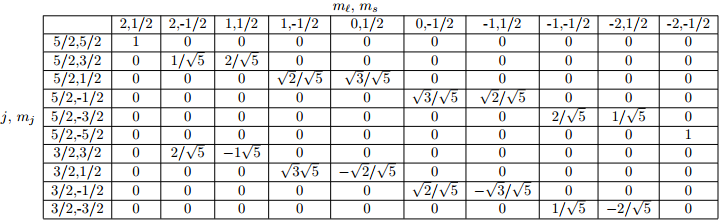
\includegraphics[width=0.7\textwidth]{figures/CG1}
			\caption{The Clebsch-Gordan coefficients for an electron with $l=2$.}
			\label{fig:CG}
		\end{figure}
		
		\item \emph{Summarize your result in terms of Clebsch-Gordan coefficients.}\newline
		
		The Clebsch-Gordan\index{Clebsch-Gordon coefficients} coefficients are the coefficients on the right hand side of $\ket{j,m}=..\ket{m_1,m_2}+...\ket{m_1,m_2}...$. These are given by
		\begin{equation}
			\begin{split}
				&\braket{m_1=2,m_2=\frac{1}{2}|j=\frac{5}{2},m=\frac{5}{2}}=1,\\
				&\braket{m_1=1,m_2=\frac{1}{2}|j=\frac{5}{2},m=\frac{3}{2}}=\sqrt{\frac{4}{5}},\\
				&\braket{m_1=2,m_2=-\frac{1}{2}|j=\frac{5}{2},m=\frac{3}{2}}=\sqrt{\frac{1}{5}},\\
				&\braket{m_1=1,m_2=\frac{1}{2}|j=\frac{3}{2},m=\frac{3}{2}}=-\sqrt{\frac{1}{5}},\\
				&\braket{m_1=2,m_2=-\frac{1}{2}|j=\frac{3}{2},m=\frac{3}{2}}=\sqrt{\frac{4}{5}}.\\
			\end{split}
		\end{equation} 
		
	\end{enumerate}
\end{example}


\chapter{Approximation methods}


\section{Perturbation theory in QM}
\label{chp:TDPT}
In the preceding chapters I have illustrated how to solve some simple quantum mechanical systems exactly. Most quantum mechanical systems, however, cannot be solved exactly, and so instead approximate methods are used. One such method is perturbation theory. In the words of Paul Dirac~\citep[p.167]{dirac} 

\begin{quote}
	“\textit{... Most quantum problems, however, cannot be solved exactly with the present resources of mathematics, as they lead to equations whose solutions cannot be expressed in finite terms with the help of the ordinary functions of analysis. For such problems one can often use a perturbation method. This consists in splitting up the Hamiltonian into two parts, one of which must be simple and the other small. The first part may then be considered as the Hamiltonian of a simplified or unperturbed system, which can be dealt with exactly, and the addition of the second will then require small corrections, of the nature of a perturbation, in the solution for the unperturbed system. The requirement that the first part shall be simple requires in practice that it shall not involve the time explicitly.}”
\end{quote} 

That is in perturbation theory one assume that the Hamiltonian of the system under consideration can be described by a known Hamiltonian plus a relatively small perturbative Hamiltonian. The method of procedure for determining the energy levels and eigenstates of the Hamiltonian depends on whether or not the energy levels of the Hamiltonian are degenerate and whether or not the perturbative Hamiltonian depends on time. In this chapter I will review how to deal with the different cases.

\subsection*{Non-degenerate, time-independent perturbation theory}
\index{TIPT, non-deg.}
Non-degenerate, time-independent perturbation theory deals with the case where the perturbative Hamiltonian is time-independent. Since the non-perturbative Hamiltonian always is considered time independent, this means that the total Hamiltonian is considered time independent in this case. The total Hamiltonian is taken to be on the form
\begin{equation}
	H=H_0+\lambda H',
	\label{ham13}
\end{equation} 
where $0\leq\lambda\leq1$ is a parameter, representing the strength of the perturbation, that is introduced for book-keeping purposes.  $H_0$ is the unperturbed Hamiltonian. It is assumed that the eigenstates and eigenvalues of the unperturbed Hamiltonian is known
\begin{equation}
	H_0\ket{n^0}=E_n^{(0)}\ket{n^0}.
\end{equation} 
Since the total Hamiltonian is time independent, separation of variables can be used to separate the Schroedinger equation into a time-dependent and time-independent equation. Since I have already solved the time-dependent one, I will focus on the time-independent one here. This will be on the form
\begin{equation}
	H\ket{n}=E_n\ket{n}.
	\label{ham12}
\end{equation} 
The perturbation changes $\ket{n^0}$ only slightly, and therefore the new eigenstate can be expanded in terms of $\ket{n^0}$. In mathematical terms; the perturbation does not change the Hilbert space, so the eigenvectors of the unperturbed Hamiltonian can be used to expand the eigenvectors of the total Hamiltonian. Since the perturbation is assumed only to change the state slightly I will describe a given eigenstate of the total Hamiltonian as the corresponding eigenstate of the unperturbed Hamiltonian plus some perturbative term
\begin{equation}
	\ket{n}=\ket{n^0}+\ket{\Delta n},
\end{equation} 
where the perturbative term can be expanded in terms of the eigenvectors of the unperturbed Hamiltonian (minus the eigenvector $\ket{n^0}$ since this is already used)
\begin{equation}
	\ket{\Delta n}=\sum_{k\neq n}^{}c_k\ket{k^0}.
\end{equation} 
Similarly the energy of a given eigenstate can be described as the energy of the corresponding eigenstate of the unperturbed Hamiltonian plus some perturbative term
\begin{equation}
	E_n=E_n^{(0)}+\Delta E_n.
\end{equation} 
The aim of perturbation theory is to determine $\Delta E_n$ and $\ket{\Delta n}$ so the eigenstates and eigenvalues of the total Hamiltonian is determined. To this end I insert the expression for $E_n$ and $\ket{n}$ into equation \eqref{ham12}. Thereby
\begin{equation}
	(H_0+\lambda H')(\ket{n^0}+\ket{\Delta n})=(E_n^{(0)}+\Delta E_n)(\ket{n^0}+\ket{\Delta n}).
	\label{eq19}
\end{equation} 
I let the first terms on the LHS and RHS\footnote{LHS=Left Hand Side, RHS=Righ Hand Side.} cancel and act from the left with the bra $\bra{n^0}$. Since $\braket{n^0|n'^0}=\delta_{n^0 n'^0}$, and $\ket{\Delta n}$ is expanded in terms of $\ket{k^0}$ where $k\neq n$, $\braket{n^0|\Delta n}=0$ and $\braket{n^0|n^0}=1$. For the third term on the LHS of equation \eqref{eq19} I use that $H_0$ is Hermitian and I can therefore let it operate to the left onto its eigenstate and obtain the eigenvalue. Since the eigenvalue is just a number the bra is allowed to operator onto the ket, but since $\braket{n^0|\Delta n}=0$ the term vanishes. On the RHS I can let the bra operate onto the kets immediately since the eigenvalues are just numbers and numbers commute with all operators. Therefore the two last terms cancel using again that $\braket{n^0|\Delta n}=0$. Thus I am left with
\begin{equation}
	\lambda\braket{n^0|H'|n}=\Delta E_n,
	\label{eq20}
\end{equation} 
where I have used that $\lambda\bra{n^0}H'\ket{n^0}+\lambda\bra{n^0}H'\ket{\Delta n}=\lambda\braket{n^0|H'|n}$. The effect of the perturbation is to shift the energy level (originally $E_n$) by an amount $\Delta E_n$ which can be determined by equation \eqref{eq20}. However, to calculate the shift in the energy the state $\ket{n}$ has to be determined. In reality it is expanded in powers of $\lambda$
\begin{equation}
	\begin{split}
		\ket{n}&=\sum_{i}\lambda^i\ket{n^i}\\
		&=\ket{n^0}+\lambda\ket{n^1}+\lambda^2\ket{n^2}+...\\
		&=\ket{n^0}+\lambda\sum_{k\neq n}^{}c_k^{(1)}\ket{k^0}+\lambda^2\sum_{k\neq n}^{}c_k^{(2)}\ket{k^0}+....
		\label{eig4}
	\end{split}
\end{equation} 
Each of the terms $\lambda^i\ket{n^i}$ are correction terms that add up to $\ket{\Delta n}$. Since the expansion of$\ket{\Delta n}$ on $\ket{k^0}$ was for a general vector that was not $n^0$ the same method applies for each of the vectors $\ket{n^i}$. 
By inserting this power series expansion into equation \eqref{eq20} the shift in energy can be written as
\begin{equation}
	\begin{split}
		\Delta E_n&=\lambda\braket{n^0|H'|n^0}+\lambda^2\braket{n^0|H'|n^1}+\lambda^3\braket{n^0|H'|n^2}+...\\
		&=\sum_{i}\lambda^i\braket{n^0|H'|n^{(i-1)}}\\
		&=\sum_{i}\lambda^iE_n^i,
	\end{split}
	\label{eq21}
\end{equation} 
where I have defined $\braket{n^0|H'|n^{(i-1)}}=E_n^i$. Therefore also the energy change can be described in terms of a power series in the energy\footnote{Note that the expansion of the energy can be written as $E_n=E_n^{(0)}+\lambda E_n^{(1)}+...$.}. By using the power series expansions of the energy and the state in equation \eqref{ham12} I find
\begin{equation}
	\begin{split}
		&\bigg(H_0+\lambda H'\bigg)\bigg(\ket{n^0}+\lambda\sum_{k\neq n}^{}c_k^{(1)}\ket{k^0}+\lambda^2\sum_{k\neq n}^{}c_k^{(2)}\ket{k^0}+...\bigg)\\&=\bigg(E_n^{(0)}+\lambda E_n^{(1)}+...\bigg)\bigg(\ket{n^0}+\lambda\sum_{k\neq n}^{}c_k^{(1)}\ket{k^0}+\lambda^2\sum_{k\neq n}^{}c_k^{(2)}\ket{k^0}+...\bigg).
	\end{split}
\end{equation} 
I then compare the terms of equal order of $\lambda$
\begin{equation}
	\begin{split}
		&\lambda^0:\qquad H_0\ket{n^0}=E_n^{(0)}\ket{n^0},\\
		&\lambda^1:\quad \sum_{k\neq n}^{}c_k^1H_0\ket{k^0}+H'\ket{n^0}=E_n^{(0)}\sum_{k\neq n}^{}c_k^{(1)}\ket{k^0}+E_n^{(1)}\ket{n^0},\\
		&\lambda^2:\quad \sum_{k\neq n}^{}c_k^{(2)}H_0\ket{k^0}+\sum_{k\neq n}^{}c_k^{(1)}H'\ket{k^0}=E_n^{(0)}\sum_{k\neq n}^{}c_k^{(2)}\ket{k^0}+E_n^{(1)}\sum_{k\neq n}^{}c_k^{(1)}\ket{k^0}+E_n^{(2)}\ket{n^0}.
	\end{split}
	\label{eq22}
\end{equation} 
The $0$'th order term just returns the unperturbed, TI Schroedinger equation - this is a good thing, as the system should to the $0$'th order not be perturbed! For the first order term I act with $\bra{n^0}$ from the left to find the first order correction to the energy
\begin{equation}
	\begin{split}
		\lambda^1:\qquad E_n^{(1)}&=\frac{\braket{n^0|H'|n^0}}{\braket{n^0|n^0}}\\
		&=\int\int\braket{n^0|x'}\braket{x'|H'|x''}\braket{x''|n^0}d^3x'd^3x''\\
		&=\int|\braket{n^0|x'}|^2\braket{x'|H'|x'}d^3x',
	\end{split}
\end{equation} 
where if the states are normalized $\braket{n^0|n^0}=1$. For the second order term I do the same from which I find
\begin{equation}
	\lambda^2:\qquad E_n^{(2)}=\sum_{k\neq n}c_k^{(1)}\frac{\braket{n^0|H'|k^0}}{\braket{n^0|n^0}}=\sum_{k\neq n}c_k^{(1)}\braket{n^0|H'|k^0},
\end{equation} 
where I have assumed the states are normalized in the above equality (i.e. that $\braket{n'|n}=\delta_{n'n}$). $c_k^1$ is determined by acting with $\bra{k'^0}$ from the left on equation \eqref{eq22}. Hereby
\begin{equation}
	\lambda^1:\qquad \braket{k'^0|H'|n^0}+c_{k'}^{(1)}E_{k'}^{(1)}=E_n^{(0)}c_{k'}^{(1)} \Rightarrow c_{k'}^{(1)}=\frac{\braket{k'^0|H'|n^0}}{E_n^{(0)}-E_{k'}^{(0)}}.
\end{equation} 
$k'$ is just a dummy index, so I let $k'\Rightarrow k$ and use the above in the second order correction to the energy. Thereby
\begin{equation}
	\lambda^2:\qquad E_n^{(2)}=\sum_{k\neq n}\frac{|\braket{k^0|H'|n^0}|^2}{E_n^{(0)}-E_k^{(0)}}.
\end{equation} 
Collecting the first and second order correction
\begin{equation}
	\Delta E_n=\sum_{i}\lambda^iE_n^i=\lambda \braket{n^0|H'|n^0}+\lambda^2\sum_{k\neq n}\frac{|\braket{k^0|H'|n^0}|^2}{E_n^{(0)}-E_k^{(0)}}+....
\end{equation} 
Likewise for the eigenstate
\begin{equation}
	\ket{n}=\sum_{i}\lambda^i\ket{n^i}=\ket{n^0}+\lambda\sum_{k\neq n}^{}\frac{\braket{k^0|H'|n^0}}{E_n^{(0)}-E_{k}^{(0)}}\ket{k^0}+....
\end{equation} 
In the end, which this is, the strength of the perturbation is set to unity (i.e. $\lambda=1$). Thereby
\begin{equation}
	\Delta E_n=\underbrace{\braket{n^0|H'|n^0}}_{\mathcal{O}(\lambda)}+\underbrace{\sum_{k\neq n}\frac{|\braket{k^0|H'|n^0}|^2}{E_n^{(0)}-E_k^{(0)}}}_{\mathcal{O}(\lambda^2)}+...,
	\label{correction energy}
\end{equation} 
\begin{equation}
	\ket{n}=\underbrace{\ket{n^0}}_{\mathcal{O}(\lambda^0)}+\underbrace{\sum_{k\neq n}^{}\frac{\braket{k^0|H'|n^0}}{E_n^{(0)}-E_{k}^{(0)}}\ket{k^0}}_{\mathcal{O}(\lambda)}+....
	\label{correction state}
\end{equation} 
Even through the $\lambda$'s are gone, one must remember where they were because they describe the order of the perturbative term! By collecting higher orders of lambda and sandwiching from the left with a bra higher order corrections to the energy and state vector can be found. However, the first corrections provides a very good approximation in most cases and so higher order terms are not needed\footnote{The expressions also gets increasingly more complicated. If the expressions were simpler perhaps they would have been incorporated. A funny side note: P. A. M. Dirac was almost religious in the belief that math describing physical phenomena should be beautiful". He would dismiss a physical theory on the basis of the mathematics being "not beautiful". This has frustrated many physicists pitching ideas to him.}\footnote{Dirac is the inventor of TDPT - this is perhaps why it is well explained!}.

\subsection*{Degenerate, time-independent perturbation theory}
\index{TIPT, deg.}
In the case of degenerate energy levels the same equations cannot be used since the denominators (in the $\lambda^2
$ and $\lambda$ term respectively) in equation \eqref{correction energy} and \eqref{correction state} blow up if $E_n^0=E_k^0$. An infinity hints that the physics are wrong, and indeed they are in this case. The error comes from the eigenstate. From equation \eqref{correction state} it is clear that the correction to a given eigenstate is taken as a perturbation with respect to a state that refers to the energy level. However, in the case of degeneracy several eigenstates can be $\ket{n^0}$. To fix this I use that a linear combination of the degenerate states is orthogonal to the non-degenerate states. I denote the set of degenerate states as $g$ and the individual degenerate eigenvectors as $\ket{m^0}$\footnote{So the different eigenvectors $\ket{m^0}$ are the elements in the set of degenerate eigenvectors; $g$.}. From these definitions I can write a degenerate version of equation \eqref{eig4} as follows
\begin{equation}
	\ket{n}=\sum_{m\in g}x_m\ket{m^0}+\lambda\sum_{k\not\in g}c_k^{(1)}\ket{k^0}+\lambda^2\sum_{k\not\in g}c_k^{(2)}\ket{k^0}+....
	\label{correction state1}
\end{equation} 
where $x_m$ is just the set of expansion coefficients amongst the degenerate eigenstates. I use the same procedure as in the non-degenerate case and so I must also represent the energy by an expansion in powers of $\lambda$. Since I have fixed the issue (the degeneracy of $\ket{n^0}$) I can use the same expansion as in the non-degenerate case
\begin{equation}
	E_n=E_n^{(0)}+\lambda E_n^{(1)}+\lambda^2E_n^{(2)}+....
\end{equation} 
By using these in the TI Schroedinger equation (equation \eqref{ham12}) alongside the definition of the Hamiltonian from equation \eqref{ham13}
\begin{equation}
	\begin{split}
		&\bigg(H_0+\lambda H'\bigg)\bigg(\sum_{m\in g}x_m\ket{m^0}+\lambda\sum_{k\not\in g}c_k^{(1)}\ket{k^0}+\lambda^2\sum_{k\not\in g}c_k^{(2)}\ket{k^0}+...\bigg)\\
		&=\bigg(E_n^{(0)}+\lambda E_n^{(1)}+\lambda^2E_n^{(2)}+...\bigg)\bigg(\sum_{m\in g}x_m\ket{m^0}+\lambda\sum_{k\not\in g}c_k^{(1)}\ket{k^0}+\lambda^2\sum_{k\not\in g}c_k^{(2)}\ket{k^0}+\dots\bigg).
	\end{split}
\end{equation} 
I compare the terms of the same order in $\lambda$
\begin{equation}
	\begin{split}
		&\lambda^0:\quad \sum_{m\in g}x_mH_0\ket{m^0}=E_n^{(0)}\sum_{m\in g}x_m\ket{m^0},\\
		&\lambda^1:\quad \sum_{m\in g}x_mH'\ket{m^0}+\sum_{k\not\in g}c_k^{(1)}E_k^{(0)}\ket{k^0}=E_n^{(0)}\sum_{k\not\in g}c_k^{(1)}\ket{k^0}+E_n^{(1)}\sum_{m\in g}x_m\ket{m^0},\\
		&\lambda^2:\quad \sum_{k\not\in g}c_k^{(1)}H'\ket{k^0}+\sum_{k\not\in g}c_k^{(2)}E_k^{(0)}\ket{k^0}
		=E_n^{(0)}\sum_{k\not\in g}c_k^{(2)}\ket{k^0}+E_n^{(1)}\sum_{k\not\in g}c_k^{(1)}\ket{k^0}+E_n^{(2)}\sum_{m\in g}x_m\ket{m^0},
	\end{split}
\end{equation} 
where $H_0\ket{m^0}=E_n^{(0)}\ket{m^0}$. By acting from the left with $\bra{m'^0}$ I find\footnote{Nothing exciting happens for the zeroth order term.}
\begin{equation}
	\lambda^1:\qquad \sum_{m\in g}x_m\bra{m'^0}H'\ket{m^0}=E_n^{(1)}x_{m'}.
\end{equation} 
This is a matrix equation on the same form as equation \eqref{matrixeig1}. Cf. Cramers rule there only exists non-trivial solutions if
\begin{equation}
	det(H'-E_n^{(1)}I)=0 \Rightarrow \{E_n^{(1)}\}, \{\ket{l}\}.
\end{equation} 
Diagonalizing the matrix $H'$\footnote{In practice the matrix to be diagonalized is the matrix containing the entire extra term, that is including $\lambda$.} results in $E_n^{(1)}$ and $x_m$.\footnote{The different sets of $x_m$ in turn results in the eigenvectors, $\ket{l}$, corresponding to the eigenvalues, $E_n^{(1)}$.} Since the number of eigenvalues match the dimensions of the matrix, there will be several, different, corrections to the degenerate energy level. This is to be understood as the degenerate energy level splitting into distinct energy levels; the perturbation splits the degenerate energy level into distinct energy levels.  
\begin{figure}[ht]
	\captionsetup{width=1\textwidth}
	\centering
	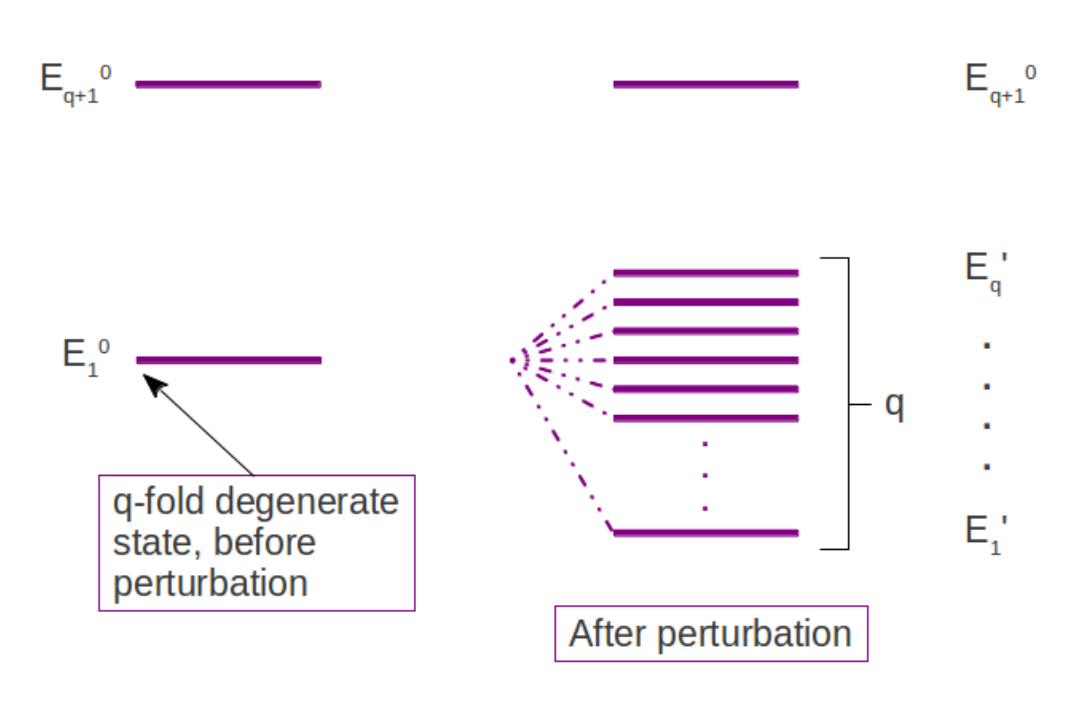
\includegraphics[width=0.6\textwidth]{figures/degpert}
	\caption{The splitting of the degenerate energy level.}
	\label{fig:degpert}
\end{figure}
Since there can be degeneracy in the energy levels when diagonalizing a matrix, the diagonalization does not guarantee a complete lifting of the degeneracy. I will however limit myself to the case where this is so. If I lift the degeneracy I can use the same formulas, with the correction that the sum is only over non-degenerate energy eigenstates, as in the non-degenerate case to determine the higher order correction. Thereby I in the end find
Collecting the first and second order correction
\begin{equation}
	\Delta E_n=\underbrace{E_n^{(1)}}_{\mathcal{O}(\lambda)}+\underbrace{\sum_{k\notin g}\frac{|\braket{k^0|H'|n^0}|^2}{E_n^{(0)}-E_k^{(0)}}+}_{\mathcal{O}(\lambda^2)}..., 
	\label{correction energy2}
\end{equation} 
where $E_n^{(1)}$ are the eigenvalues of the degenerate perturbation matrix and can take different values. The second order correction is the same for each of these different values of $E_n^{(1)}$. For the eigenstate
\begin{equation}
	\ket{n}=\underbrace{\ket{l}}_{\mathcal{O}(\lambda^0)}+\underbrace{\sum_{k \notin g}\frac{\bra{k^0}\mathcal{H}'\ket{l}}{E_l^{0}-E_k^{0}}\ket{k^{0}}}_{\mathcal{O(\lambda)}}+...,
	\label{correction state2}
\end{equation} 
where $\ket{l}$ are any of the eigenvectors obtained from diagonalizing the degenerate sub-matrix of the perturbative Hamiltonian. By comparison between equation \eqref{correction energy} versus \eqref{correction energy2} and equation \eqref{correction state} versus \eqref{correction state2} it is clear that the corrections in degenerate perturbation theory are reminiscent of the ones from non-degenerate perturbation theory. The procedure in degenerate perturbation theory is to find the basis in which the sub-matrix of the perturbative Hamiltonian that is degenerate is diagonal. If this basis lifts the degeneracy completely the non-degenerate perturbation theory can be applied to the eigenstates and eigenvalues of the degenerate perturbation matrix.  

\subsection*{Time-dependent perturbation theory}
\index{TDPT}
Time-dependent perturbation theory is an approximate method for solving the Schroedinger equation in the case where $\frac{\partial H}{\partial t}\neq0$ - that is in the case where separation of variables does not apply. The Hamiltonian is taken to consist of two additive parts; one simple part ($H_0$) for which the solution is known and one smaller part ($H'$). The simple part must contain any time dependency in order to be simple($\frac{\partial H_0}{\partial t}=0$), so the time dependency of the Hamiltonian must lie in the small part, i.e. $H'=H'(t)$. The Hamiltonian is therefore given by
\begin{equation}
	H=H_0+H'(t).
\end{equation} 
The system is taken to be in an eigenstate of $H_0$ at $t=0s$. In some finite interval of time the system is then perturbed, in this case the system is a nucleus, and the perturbation is scattering with the WIMP. After the perturbation, the system is again characterized by the simple Hamiltonian, and the system is possibly in the same or a different eigenstate of the simple Hamiltonian. The scenario is shown in figure \ref{fig:jj}.
\begin{figure}[ht]
	\captionsetup{width=1\textwidth}
	\centering
	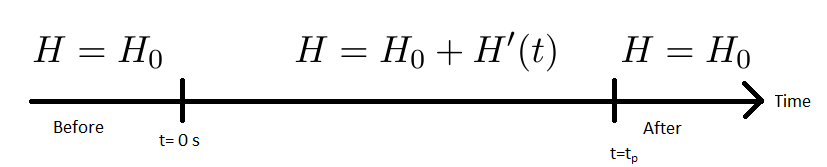
\includegraphics[width=1\textwidth]{figures/tipertub}
	\caption{The development of the Hamiltonian as a function of time.}
	\label{fig:jj}
\end{figure}
While the perturbation is turned on ($0\leq t\leq t_p$) the system is described by the Schroedinger equation on the form
\begin{equation}
	i\hbar\frac{\partial \ket{\alpha}}{\partial t}=(H_0+H'(t))\ket{\alpha},
	\label{sch4}
\end{equation} 
where $\ket{\alpha}$ is the state-vector. Equation \eqref{sch4} is solved by assuming that the eigenvectors and eigenvalues of the unperturbed system is known. Since the unperturbed Hamiltonian is time independent the Schroedinger equation can in this case be solved via separation of variables. The time-dependent Schroedinger equation is trivially solved while the time-independent Schroedinger equation is given by
\begin{equation}
	H_0\ket{n_0}=E_{n_0}\ket{n_0},
\end{equation}  
where $E_{n_0}$ and $\{\ket{n_0}\}$ is taken to be known. Since the eigenvectors of $H_0$ make up a complete set, spanning the desired vector space, they are used to develop the state-vector of the system
\begin{equation}
	\ket{\alpha}=\sum_{n_0}^{}c_{n_0}(t)e^{-\frac{iE_{n_0}}{\hbar}t}\ket{n_0},
	\label{expansion2}
\end{equation}  
where, compared to the case where the Hamiltonian is time-independent, the coefficients of the expansion are now time-dependent. The probability of the system ending up in a given state is given by the squared magnitude of the coefficients $c_{n_0}(t)$. To solve equation \eqref{sch4} equation \eqref{expansion2} is inserted
\begin{equation}
	\begin{split}
		&i\hbar\sum_{n_0}^{}\frac{\partial c_{n_0}(t)}{\partial t}e^{-\frac{iE_{n_0}}{\hbar}t}\ket{n_0}-i\hbar\sum_{n_0}^{}c_{n_0}(t)\frac{iE_{n_0}}{\hbar}e^{-\frac{iE_{n_0}}{\hbar}t}\ket{n_0}=\sum_{n_0}^{}(H_0+H'(t))\ket{n_0}c_{n_0}(t)e^{-\frac{iE_{n_0}}{\hbar}t}.
	\end{split}
	\label{sch5}
\end{equation} 
Equation \eqref{sch5} is multiplied from the left with a eigenbra of $H_0$; $\bra{m_{0}}$
\begin{equation}
	\begin{split}
		&	i\hbar\sum_{n_0}^{}\frac{\partial c_{n_0}(t)}{\partial t}e^{-\frac{iE_{n_0}}{\hbar}t}\braket{m_0|n_0}+\sum_{n_0}^{}c_{n_0}(t)E_{n_0}e^{-\frac{iE_{n_0}}{\hbar}t}\braket{m_0|n_0}\\
		&=\sum_{n_0}^{}\bra{m_0}(H_0+H'(t))\ket{n_0}c_{n_0}(t)e^{-\frac{iE_{n_0}}{\hbar}t}.
	\end{split}
	\label{sch6}
\end{equation} 
By using $\braket{m_0|n_0}=\delta_{m_0n_0}$ the sums on the left hand side vanishes. Furthermore $H_0$ operating to the right on $\ket{n_0}$  results in $E_{n_0}\ket{n_0}$ since $\ket{n_0}$ is an eigenstate of $H_0$. Since $E_{n_0}$ is just a number, it can be taken outside the inner product, and again the orthogonality property can be used to kill the sum. In the end
\begin{equation}
	\begin{split}
		&	i\hbar\frac{\partial c_{m_0}(t)}{\partial t}e^{-\frac{iE_{m_0}}{\hbar}t}+c_{m_0}(t)E_{m_0}e^{-\frac{iE_{m_0}}{\hbar}t}=c_{m_0}(t)E_{m_0}e^{-\frac{iE_{m_0}}{\hbar}t}+\sum_{n_0}^{}\bra{m_0}H'(t)\ket{n_0}c_{n_0}(t)e^{-\frac{iE_{n_0}}{\hbar}t}.
	\end{split}
	\label{sch7}
\end{equation} 
Two of the terms cancel out. By moving the exponential from the left hand side (LHS) to the right hand side (RHS)
\begin{equation}
	i\hbar\frac{\partial c_{m_0}(t)}{\partial t}=\sum_{n_0}^{}\bra{m_0}H'(t)\ket{n_0}c_{n_0}(t)e^{i\omega_{m_0n_0}t},
	\label{sch8}
\end{equation} 
where $\omega_{m_0n_0}=\frac{E_{m_0}-E_{n_0}}{\hbar}$. A general solution to equation \eqref{sch8} is difficult, but in the case where $H'\ll H_0$ perturbation theory is applicable, and an approximative solution can be found. A dimensionless, continuous, real parameter, $\lambda \in[0,1]$, representing the strength of the perturbation, is defined by
\begin{equation}
	H'(t)\Rightarrow\lambda H'(t).
\end{equation} 
$\lambda$ is "dialed" from $0$ to $1$ in a smooth, continuous way as the state of the system goes from $\ket{n_0}$ to $\ket{\alpha}$. The parameter makes sure that there is a continuous transition between the two states of the system. Next up the expansion coefficients, $c_{m_0}(t)$ and $c_{n_0}(t)$, are expanded in powers of $\lambda$
\begin{equation}
	c_{m_0}(t)=c^{(0)}_{m_0}(t)+\lambda c^{(1)}_{m_0}(t)+\lambda^2c^{(2)}_{m_0}(t)+...,
	\label{power1}
\end{equation} 
\begin{equation}
	c_{n_0}(t)=c^{(0)}_{n_0}(t)+\lambda c^{(1)}_{n_0}(t)+\lambda^2c^{(2)}_{n_0}(t)+...,
	\label{power2}
\end{equation} 
where the superscript "${(0)}$"denotes unperturbed quantities, and higher numbers identify corrections of higher orders. If the method is to be of practical interest, a good approximation must be obtained by taking only one or two terms into account. Equation \eqref{power1} and \eqref{power2} is inserted in equation \eqref{sch8}
\begin{equation}
	\begin{split}
		&i\hbar\bigg(\frac{\partial c^0_{m_0}(t)}{\partial t}+\lambda\frac{\partial c^1_{m_0}(t)}{\partial t}+\lambda^2\frac{\partial c^2_{m_0}(t)}{\partial t}+...\bigg)\\
		& =\sum_{n_0}^{}(c^0_{n_0}(t)+\lambda c^1_{n_0}(t)+\lambda^2c^2_{n_0}(t)+...)\lambda e^{i\omega_{m_0n_0}t}\bra{m_0}H'(t)\ket{n_0},
	\end{split}
	\label{sch9}
\end{equation} 
\normalsize
where the $\lambda$ outside the parenthesis on the right hand side stems from $H'(t)$. Comparing powers of $\lambda$
\begin{equation}
	\begin{split}
		&\lambda^0:\qquad \qquad \qquad \quad i\hbar\frac{\partial c^{(0)}_{m_0}(t)}{\partial t}=0\Rightarrow c^{(0)}_{m_0}(t)=const,\\
		&\lambda^1:\qquad i\hbar\frac{\partial c^{(1)}_{m_0}(t)}{\partial t}=\sum_{n_0}^{}c^{(0)}_{n_0}(t) e^{i\omega_{m_0n_0}t}\bra{m_0}H'(t)\ket{n_0},\\
		&\lambda^2:\qquad i\hbar\frac{\partial c^{(2)}_{m_0}(t)}{\partial t}=\sum_{n_0}^{}c^{(1)}_{n_0}(t) e^{i\omega_{m_0n_0}t}\bra{m_0}H'(t)\ket{n_0}.\\
	\end{split}	
	\label{c2}
\end{equation} 
It is clear that the coefficients on the LHS and RHS not are of the same power - there is a recursion relation. The coefficient $c^{(1)}_{m_0}(t)$ describes the process in which a single photon is absorbed or emitted by an atom. Higher order coefficients correspond to processes incorporating more photons (eg. $c^{(2)}_{m_0}(t)$ corresponds to a two photon process). Because the relation between the coefficients is recursive the lower order coefficients must be determined in order to determine a higher order coefficient. Therefore, to get started, $c^0_{m_0}(t)$ is determined from an analysis of the initial conditions. The system is taken to be in an eigenstate of $H_0$ denoted by $\ket{a_0}$ at $t=0$ - where $i$ is just a random label. Since the system at $t=0$ is in an eigenstate of $H_0$, the only non-zero coefficient must be the one corresponding to $\ket{a_0}$,  i.e.
\begin{equation}
	t=0: \qquad c_{a_0}=1 \quad \wedge \quad c_{i\neq a_0}=0.
	\label{initial condition}
\end{equation} 
The coefficients of 0'th order, $c^{(0)}_{n_0}(t)$, refers to the initial, unperturbed state. The only coefficient differing from 0 is $c^{(0)}_{a_0}(t)=1$. Thereby the sum in the expression for the first order coefficient can be removed and, by denoting the final state $\bra{b_0}$
\begin{equation}
	i\hbar\frac{\partial c^{(1)}_{b_0}(t)}{\partial t}=e^{i\omega_{b_0a_0}t}\bra{b_0}H'(t)\ket{a_0}.
\end{equation} 
Moving $i\hbar$ to the RHS, and integrating
\begin{equation}
	c^{(1)}_{b_0}(t)=\frac{1}{i\hbar}\int_{0}^{t}\bra{b_0}H'(t')\ket{a_0}e^{i\omega_{b_0a_0}t'}dt',
	\label{coef}
\end{equation} 
where often $t_p$ is denoted by $t$. Using equation \eqref{coef} in equation \eqref{c2}
\begin{equation}
	\begin{split}
		c^{(2)}_{b_0}(t)&=\frac{1}{i\hbar}\sum_{n_0}^{}\int_{0}^{t}c^{(1)}_{n_0}(t'') e^{i\omega_{b_0n_0}t''}\bra{b_0}H'(t'')\ket{n_0}dt'
		\\
		&=-\frac{1}{\hbar^2}\sum_{n_0}\int_{0}^{t}\bra{b_0}H'(t'')\ket{n_0}e^{i\omega_{b_0n_0}t''}\int_{0}^{t''}\bra{n_0}H'(t')\ket{a_0}e^{i\omega_{n_0a_0}t'}dt'dt''.
		\\
	\end{split}
	\label{second order}
\end{equation} 
The transition probability, via a general process, is given by
\begin{equation}
	\mbox{Transition probability from $\ket{a_0}$ to $\ket{b_0}$}=P_{a_0\Rightarrow b_0}=|c^{(1)}_{b_0}(t)+c^{(2)}_{b_0}(t)+...|^2.
	\label{trans prob}
\end{equation} 
The transition probability for an $i$-photon process, eg. single photon or tw-photon, is given by
\begin{equation}
	P^{(i)}_{a_0\Rightarrow b_0}=|c^{(i)}_{b_0}(t)|^2.
\end{equation} 
The transition probability depends on the nature of $H'(t)$. Calculating the transition probability concludes time-dependent perturbation theory(TDPT). Since the system state before perturbation is known, what is of interest is what happens to the system during the perturbation - whether or not the system jumps into another state. This probability depends on the size of the perturbation, and if the perturbation is small, the probability can be calculated from equation \eqref{trans prob}. 

\section{The WKB approximation}
The WKB method is a technique for obtaining approximate solutions to the time-independent Schroedinger equation ($\frac{\partial H}{\partial t}=0$) in one dimension\footnote{The same technique can be applied to many other differential equations.}. It is particularly useful in calculating bound state energies and tunneling rates through a potential barrier, and is for this reason used in astrophysics when dealing with the tunneling probability relevant for fusion processes. \newline
I begin with the one-dimensional Schroedinger equation in the position basis
\begin{equation}
	-\frac{\hbar^2}{2M}\frac{\partial^2\psi(x)}{\partial x^2}+V(x)\psi(x)=E\psi(x).
	\label{sch10}
\end{equation} 
This equation can be rewritten as
\begin{equation}
	\frac{\partial^2\psi(x)}{\partial x^2}=-\frac{2M(E-V(x))}{\hbar^2}\psi(x)=-\frac{p^2}{\hbar^2}\psi(x),
	\label{sch11}
\end{equation} 
where $p=\sqrt{2M(E-V(x))}$ is the classical momentum of a particle moving in a one-dimensional potential~\citep[p.346]{Griffiths}, $V(x),$ with energy $E$, provided that $E\geq V(x)$ for all $x$. where the wave function in general is a complex number, and therefore can be written as
\begin{equation}
	\psi(x)=A(x)e^{i\phi(x)},
\end{equation} 
where $\phi(x)$ is the phase of the complex number. By this notation equation \eqref{sch11} becomes
\begin{equation}
	\begin{split}
		&\bigg(\frac{\partial^2A(x)}{\partial x^2}+2i\frac{\partial A(x)}{\partial x}\frac{\partial \phi(x)}{\partial x}+iA(x)\frac{\partial^2\psi(x)}{\partial x^2}-A(x)\bigg(\frac{\partial \phi(x)}{\partial x}\bigg)^2\bigg)e^{i\phi(x)}\\
		&=-\frac{p^2}{\hbar^2}A(x)e^{i\phi(x)}.
	\end{split}
	\label{sch12}
\end{equation} 
This is equivalent to two real equations, one for the real part and one for the imaginary part. For the real part
\begin{equation}
	\frac{\partial^2A(x)}{\partial x^2}=A(x)\bigg(\bigg(\frac{\partial\phi(x)}{\partial x}\bigg)^2-\frac{p^2}{\hbar^2}\bigg).
	\label{sch13}
\end{equation} 
For the imaginary part
\begin{equation}
	\frac{\partial}{\partial x}\bigg(A(x)^2\frac{\partial \phi(x)}{\partial x}\bigg)=0.
	\label{sch14}
\end{equation} 
Equation \eqref{sch13} and \eqref{sch14} are equivalent to the time-independent Schroedinger equation. Equation \eqref{sch14} is solved by integration. Denoting the integration constant $C^2$, I find
\begin{equation}
	A(x)=\frac{C}{\sqrt{\frac{\partial \phi(x)}{\partial x}}},
	\label{A(x)}
\end{equation} 
where $C$ is a real constant. Equation \eqref{sch13} cannot be solved in general, so an approximation is introduced; \emph{it is assumed that the amplitude varies slowly, such that $\frac{\partial^2A(x)}{\partial x^2}\approx0$}, and $\frac{\frac{\partial^2A(x)}{\partial x^2}}{A(x)}\approx0$. Thus, from equation \eqref{sch13} I find
\begin{equation}
	\frac{\partial\phi(x)}{\partial x}\approx\pm\frac{p}{\hbar},
	\label{sch15}
\end{equation} 
which is solved by integration such that
\begin{equation}
	\phi(x)\approx\pm\frac{1}{\hbar}\int p(x)dx.
	\label{phi(x)}
\end{equation} 
Any constants from this integral may be absorbed into $C$, and $C$ may therefore be complex. Thus, I find the approximate solution
\begin{equation}
	\psi(x)\simeq\frac{C}{\sqrt{p(x)}}e^{\pm\frac{i}{\hbar}\int p(x)dx}.
	\label{sol}
\end{equation} 
The general, approximate solution will be a linear combination of the plus and minus solution. From equation \eqref{sol} it is clear that the probability of finding the particle at position $x$ is given by
\begin{equation}
	|\psi(x)|^2\simeq\frac{|C|^2}{p(x)}.
	\label{prob1}
\end{equation} 
Equation \eqref{prob1} reveals that the probability of finding the particle at position $x$ is inversely proportional to the classical momentum, and thereby the particle's velocity at that point. The makes sense since if the particle has a large velocity at one point, it will not spend as much time there, and the probability of finding the particle there will be smaller.

\begin{example}
	\index{TIPT, deg.}
	\index{TIPT, SHO}
	\emph{A simple harmonic oscillator (in one dimension) is subjected to a perturbation}
	\begin{equation}
		H'=bx,
	\end{equation}  
	\emph{where $b$ is a real constant.}\newline
	
	\begin{enumerate}
		\item \emph{Calculate the energy shift of the ground state to the lowest non-vanishing order.}\newline
		
		Since the energy levels of $H_0$ (the SHO) is \emph{not} degenerate, and the perturbation does not depend on time, I use TIPT in the non-degenerate version. I use equation \eqref{correction energy} and evaluate from the "bottom". The first order correction to the energy
		\begin{equation}
			\Delta E^{(1)}_0=b\braket{0^0|x|0^0}=b\int_{-\infty}^{\infty}|\psi_0(x)|^2xdx=0,
		\end{equation} 
		where I used that $\psi_n(x)=N_nH_n\big(\sqrt{\frac{\omega M}{\hbar}}x\big)e^{\frac{-\omega M x^2}{2\hbar}}$. The second order correction to the energy
		\begin{equation}
			\Delta E_0^{(2)}=b^2\sum_{k\neq 0}\frac{|\braket{k^0|x^2|0^0}|^2}{E_0^0-E_k^0}.
		\end{equation} 
		In this case it is not so straight forward since there is an infinite number of energy levels. However, by using that $\braket{n'|x|n}=\sqrt{\frac{\hbar}{2M\omega}}(\sqrt{n}\delta_{n',n-1}+\sqrt{n+1}\delta_{n',n+1})$ I take
		\begin{equation}
			\braket{k^0|x|0}=\sqrt{\frac{\hbar}{2M\omega}}(\sqrt{n}\delta_{k,0-1}+\sqrt{0+1}\delta_{k,0+1})=\sqrt{\frac{\hbar}{2M\omega}}\delta_{k,1}.
		\end{equation} 
		By using this the second order correction can be found to be
		\begin{equation}
			\Delta E_0^{(2)}=b^2\sum_{k\neq 0}\frac{|\braket{1^0|x^2|0^0}|^2}{E_0^0-E_1^0}=-\frac{b^2}{2M\omega^2},
		\end{equation} 
		where I used that $\Delta E^0=\hbar\omega=-(E_0^0-E_1^0)$. So, the energy shift to the lowest non-vanishing order (second) is given by
		\begin{equation}
			\begin{split}
				\Delta E_0&= \braket{0^0|H'|0^0}+\sum_{k\neq 0}\frac{|\braket{k^0|H'|0^0}|^2}{E_0^0-E_k^0}+...\\&=-\frac{b^2}{2M\omega^2}+....
			\end{split}
		\end{equation} 
		
		\item \emph{Solve this problem exactly and compare with your previous result.}\newline
		
		The TISE\footnote{TI= Time Independent, SE=Schroedinger Equation.} in this case is given by
		\begin{equation}
			-\frac{\hbar^2}{2M}\frac{\partial^2 \braket{x|\alpha}}{\partial x^2}+\frac{1}{2}M\omega^2x^2\braket{x|\alpha}+bx\braket{x|\alpha}=E\braket{x|\alpha}.
		\end{equation} 
		This is a second order, non-homogeneous, non-linear, partial differential equation, and as such not an easy equation to solve\footnote{If I were to solve it I would use a generalized power series approach.}. Therefore I search for a change of variables so that the equation takes a familiar form - preferably the form of the simple harmonic oscillator! Since we have a terms with $x^2$ and one with $x$ it looks factorisable. Indeed I find 
		\begin{equation}
			\frac{1}{2}M\omega^2x^2+bx=\frac{1}{2}M\omega^2\bigg(x+\frac{b}{M\omega^2}\bigg)^2-\bigg(\frac{b}{M\omega^2}\bigg)^2.
		\end{equation} 
		Inspired by this I defined $x'=x+\frac{b}{M\omega^2}$ as a new variable. Since the derivative of $x'$ with respect to $x$ is $1$ I can write the TISE in the new variable as
		\begin{equation}
			-\frac{\hbar^2}{2M}\frac{\partial^2 \braket{x|\alpha}}{\partial x'^2}+\frac{1}{2}M\omega^2\bigg(x'^2-\bigg(\frac{b}{M\omega^2}\bigg)^2\bigg)\braket{x|\alpha}=E\braket{x|\alpha},
		\end{equation} 
		which can be rewritten as
		\begin{equation}
			-\frac{\hbar^2}{2M}\frac{\partial^2 \braket{x|\alpha}}{\partial x'^2}+\frac{1}{2}M\omega^2x'^2\braket{x|\alpha}=\bigg(E+\frac{b^2}{2M\omega^2}\bigg)\braket{x|\alpha}.
		\end{equation} 
		This is the same form as the simple harmonic oscillator with the new eigenvalue
		\begin{equation}
			E'=E+\frac{b^2}{2M\omega^2}.
		\end{equation} 
		In comparison with before
		\begin{equation}
			\Delta E_0=E-E'=-\frac{b^2}{2M\omega^2},
		\end{equation} 
		which is exactly the same result as obtained from TI perturbation theory.	
	\end{enumerate}
\end{example}


\begin{example}
	\index{TIPT, SHO}
	\emph{Consider the Hamiltonian}
	\begin{equation}
		H_0=\frac{p_x^2}{2M}+\frac{1}{2}M\omega^2x^2.
	\end{equation} 
	\emph{This Hamiltonian is subjected to a perturbation on the form}
	\begin{equation}
		H'=\frac{1}{2}\varepsilon M\omega^2 x^2.
	\end{equation} 
	\emph{What is the correction to the GS energy to second order?}\newline
	
	Since the Harmonic oscillator (in 1D) is not degenerate I will use equation \eqref{correction energy}
	\begin{equation}
		\Delta E_0=\braket{0^0|H'|0^0}+\sum_{k\neq n}\frac{|\braket{k^0|H'|0^0}|^2}{E_0^{(0)}-E_k^{(0)}}+....
	\end{equation} 
	The first order correction
	\begin{equation}
		\begin{split}
			\Delta E_0^{(1)}&=\braket{0^0|H'|0^0}\\
			&=\frac{1}{2}\varepsilon M\omega^2\braket{0^0|x^2|0^0}\\
			&=\frac{1}{2}\varepsilon M\omega^2\frac{\hbar}{2M\omega}\braket{0^0|(a^\dagger+a)^2|0^0}\\
			&=\frac{\varepsilon\hbar\omega}{4}\bigg(\braket{0^0|a^\dagger a|0^0}+\braket{0^0|a^\dagger a^\dagger|0^0}+\braket{0^0|aa^\dagger|0^0}+\braket{0^0|aa|0^0}\bigg)\\
			&=\frac{\varepsilon\hbar\omega}{4}\braket{0^0|aa^\dagger|0^0}=\frac{\varepsilon\hbar\omega}{4}.
		\end{split}
	\end{equation} 
	The second order correction
	\begin{equation}
		\Delta E_0^{(2)}=\sum_{k\neq n}\frac{|\braket{k^0|H'|0^0}|^2}{E_0^{(0)}-E_k^{(0)}}.
	\end{equation} 
	To evaluate this the matrix elements need to be evaluated. In analog with the first order correction
	\begin{equation}
		\begin{split}
			\braket{k^0|H'|0^0}&=\frac{\varepsilon\hbar\omega}{4}\bigg(\braket{k^0|a^\dagger a|0^0}+\braket{k^0|a^\dagger a^\dagger|0^0}+\braket{k^0|aa^\dagger|0^0}+\braket{k^0|aa|0^0}\bigg)\\
			&=\frac{\varepsilon\hbar\omega}{4}\bigg(\braket{k^0|a^\dagger a^\dagger|0^0}\delta_{k,2}+\braket{k^0|aa^\dagger|0^0}\delta_{k,0}\bigg)\\
			&=\frac{\varepsilon\hbar\omega}{4}\bigg(\sqrt{2}\delta_{k,2}+\delta_{k,0}\bigg).\\
		\end{split}
		\label{shit}
	\end{equation} 
	Since the sum is only over $k\neq n$ the $k=0$ is not included in the second order correction
	\begin{equation}
		\Delta E_0^{(2)}=\bigg(\frac{\sqrt{2}\varepsilon\hbar\omega}{4}\bigg)^2\frac{1}{\frac{1}{2}\hbar\omega-\frac{5}{2}\hbar\omega}=-\frac{\varepsilon^2\hbar\omega}{16}.
	\end{equation} 
\end{example}

\begin{example}
	\index{TIPT, non-deg.}
	\index{TIPT, deg.}
	\index{TIPT, free particle in a box}
	\emph{Consider a particle in a two-dimensional potential}
	\begin{equation}
		V_0=\begin{cases} 0 &\mbox{for} \quad 0\leq x\leq L, 0\leq y \leq L \\ 
			\infty & \mbox{for} \quad \mbox{Else}  
		\end{cases}. 
	\end{equation} 
	\begin{enumerate}
		\item \emph{Find the eigenfunctions for the ground state and the first excited state.}\newline
		
		This is identical to the free particle in a box in two dimensions. Taking only the TI part of $\braket{x|\alpha}=\psi(x,y,z,t)_{n_xn_yn_z}=Bsin\big(\frac{n_x\pi}{L}x\big)sin\big(\frac{n_y\pi}{L}y\big)sin\big(\frac{n_z\pi}{L}z\big)e^{-\frac{iE_{n_xn_yn_z}}{\hbar}t}$ I find
		\begin{equation}
			\braket{\vec{x}|n}=\psi(x,y)_{n_x,n_y}=\frac{2}{L}sin\bigg(\frac{n_x\pi}{L}x\bigg)sin\bigg(\frac{n_y\pi}{L}y\bigg),
		\end{equation} 
		from which
		\begin{equation}
			\begin{split}
				\psi(x,y)_{1,1}&=\frac{2}{L}sin\bigg(\frac{\pi}{L}x\bigg)sin\bigg(\frac{\pi}{L}y\bigg),\\
				\psi(x,y)_{2,1}&=\frac{2}{L}sin\bigg(\frac{2\pi}{L}x\bigg)sin\bigg(\frac{\pi}{L}y\bigg),\\
				\psi(x,y)_{1,2}&=\frac{2}{L}sin\bigg(\frac{\pi}{L}x\bigg)sin\bigg(\frac{2\pi}{L}y\bigg).\\
			\end{split}
			\label{fe}
		\end{equation} 
		
		\item \emph{Now a perturbative term is added. The perturbative terms is given by}
		\begin{equation}
			H'=\begin{cases} \lambda xy &\mbox{for} \quad 0\leq x\leq L, 0\leq y \leq L \\ 
				0 & \mbox{for} \quad \mbox{Else}  \end{cases} .
		\end{equation} 
		\emph{Obtain the zeroth order energy eigenfunctions and the first order energy shifts for the ground state and the first excited state.}\newline
		
		The GS is non-degenerate so non-degenerate perturbation theory can be used here. The first excited states are degenerate so here degenerate perturbation theory must be used (the perturbative Hamiltonian does not depend on time so TDPT is not used here).\newline 
		For the GS the zeroth order energy eigenfunction is given by equation \eqref{fe}. The first order shift to the energy is given by
		\begin{equation}
			\begin{split}
				\Delta E_{1,1}^{(1)}&= \braket{1^0|H'|1^0}\\
				&=\frac{4\lambda}{L^2}\int_{0}^{L}\int_{0}^{L}sin\bigg(\frac{\pi}{L}x\bigg)^2sin\bigg(\frac{\pi}{L}y\bigg)^2xydxdy\\
				&=\frac{L^2\lambda}{4}.
			\end{split}
			\label{FPE1}
		\end{equation} 
		For the first excited state there is degeneracy, and so degenerate perturbation theory will be used instead of non-degenerate perturbation theory. I construct the matrix $\braket{n'|H'|n}$ where $n,n'=2,1;1,2$\footnote{That is a matrix of the degenerate eigenfunctions!}. That is
		\begin{equation}
			\begin{split}
				H'&\doteq\begin{bmatrix}
					\braket{1,2|H'|1,2} & \braket{1,2|H'|2,1}\\
					\braket{2,1|H'|1,2} & \braket{2,1|H'|2,1}\\
				\end{bmatrix}\\
				&=\begin{bmatrix}
					A& B\\
					C& D\\
				\end{bmatrix}\\
				&=\frac{\lambda L^2}{4}\begin{bmatrix}
					1& \frac{1024}{81\pi^4}\\
					\frac{1024}{81\pi^4} & 1\\
				\end{bmatrix},
			\end{split}
		\end{equation} 
		where
		\begin{equation}
			\begin{split}
				&A\equiv \frac{4\lambda}{L^2}\int_{0}^{L}\int_{0}^{L} sin(\frac{\pi}{L}x)^2sin(\frac{2\pi}{L}y)^2dxdy,\\
				&B\equiv \frac{4\lambda}{L^2}\int_{0}^{L}\int_{0}^{L} sin(\frac{\pi}{L}x)sin(\frac{2\pi}{L}y)sin(\frac{2\pi}{L}x)sin(\frac{\pi}{L}y)dxdy,\\
				&C\equiv \frac{4\lambda}{L^2}\int_{0}^{L}\int_{0}^{L} sin(\frac{\pi}{L}x)sin(\frac{2\pi}{L}y)sin(\frac{2\pi}{L}x)sin(\frac{\pi}{L}y)dxdy, \\
				&D\equiv \frac{4\lambda}{L^2}\int_{0}^{L}\int_{0}^{L} sin(\frac{2\pi}{L}x)^2sin(\frac{\pi}{L}y)^2dxdy.\\		
			\end{split}
		\end{equation}
		The eigenvalues of $H'$ are the first order corrections to the energy. That is
		\begin{equation}
			\Delta E_{2,1}^{(1)}=\frac{\lambda^2L^2}{324\pi^4}(81\pi^4\pm 1024).
			\label{FPE2}
		\end{equation} 
		As is apparent from the above; the energy level of the first excited state is, to first order, split into two distinct energy states. Hence the degeneracy is lifted! \newline
		The eigenvectors of $H'$ corresponds to the zeroth order energy eigenvectors. Denoting the two energy levels the first excited energy level has split into by $E_{2,i}$ where $i=1,2$, the corresponding eigenvectors can be found to be
		\begin{equation}
			\ket{E_{2,1}}=\frac{1}{\sqrt{2}}(\ket{1,2}-\ket{2,1}),
		\end{equation} 
		\begin{equation}
			\ket{E_{2,2}}=\frac{1}{\sqrt{2}}(\ket{1,2}+\ket{2,1}).
		\end{equation} 
		
	\end{enumerate}
\end{example}

\begin{example}
	\index{TIPT, free particle in a box}
	\emph{Consider a spin-less particle in a two-dimensional infinite square well}
	\begin{equation}
		V_0=\begin{cases} 0 &\mbox{for} \quad 0\leq x\leq a, 0\leq y \leq a \\ 
			\infty & \mbox{for} \quad \mbox{Else}  \end{cases}. 
	\end{equation} 
	
	\begin{enumerate}
		\item \emph{What are the energy eigenvalues for the three lowest states? Is there any degeneracy?}\newline
		
		Inside the box the particle is treated as a free particle in two dimensions. The energy is just the sum of two free particles in a 1D box
		\begin{equation}
			E_{n_x,n_y}^{(0)}=\frac{\hbar^2\pi^2}{2ML^2}(n_x^2+n_y^2),
		\end{equation} 
		where $n_i=1,2,3...$. Note that $n_i=0$ is\emph{not} a possibility since this value would make the wave-function, which is a product of the two wave-function of a 1D free particle in a box and $\psi\propto sin(n_x)sin(n_y)$, zero. Therefore the GS is given by
		\begin{equation}
			E_{1,1}^{(0)}=\frac{\hbar^2\pi^2}{ML^2}.
		\end{equation} 
		There is no degeneracy here. The following energy states
		\begin{equation}
			E_{2,1}^{(0)}=E_{1,2}^{(0)}=\frac{5\hbar^2\pi^2}{2ML^2},
		\end{equation} 
		where there is two-fold degeneracy. \newline
		
		\item \emph{Now a perturbative potential is added}
		\begin{equation}
			H'=\lambda xy.
		\end{equation} 
		\begin{enumerate}
			\item \emph{Is the energy shift due to the perturbation linear or quadratic in $\lambda$ for each of the three states?}\newline
			
			Cf. equation \eqref{FPE1} and \eqref{FPE2} $\Delta E_{1,1}^{(1)}\propto\lambda$ and $\Delta E_{2,1}^{(1)}\propto\lambda^2$.
			
			\item \emph{Draw an energy diagram representing before and after the perturbation.}\newline
			\begin{figure}[ht]
				\captionsetup{width=1\textwidth}
				\centering
				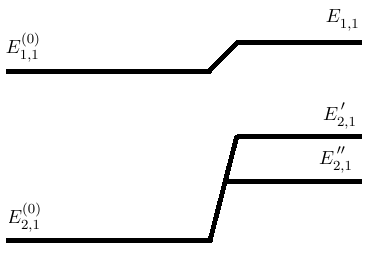
\includegraphics[width=0.4\textwidth]{figures/perturb}
				\caption{}
			\end{figure}
			
		\end{enumerate}
		
	\end{enumerate}
\end{example}


\begin{example}
	\index{TIPT, non-deg.}
	\index{TIPT, deg.}
	\index{TIPT, SHO}
	\emph{Consider an isotropic SHO in two dimensions. The Hamiltonian is}\newline
	\begin{equation}
		H=\frac{1}{2M}(p_x^2+p^2_y)+\frac{M\omega ^2}{2}(x^2+y^2).
	\end{equation} 
	\begin{enumerate}
		\item \emph{What are the energies of the three lowest-lying states? Is there any degeneracy?}\newline
		
		The energy is given by the sum of the two harmonic oscillators
		\begin{equation}
			E_{n_x,n_y}=\hbar\omega(\frac{1}{2}+n_x)+\hbar\omega(\frac{1}{2}+n_y)=\hbar \omega(1+n_x+n_y).
		\end{equation} 
		So, the lowest state
		\begin{equation}
			E_{0,0}=\hbar \omega.
		\end{equation} 
		There is no degeneracy. The next lowest level(s)
		\begin{equation}
			E_{1,0}=E_{0,1}=2\hbar \omega,
		\end{equation} 
		where there is twofold degeneracy.\newline
		
		\item \emph{Now apply the perturbation}
		\begin{equation}
			H'=\delta M\omega^2xy,
		\end{equation} 
		\emph{where $\delta\ll1$ is a real number. Find the zeroth order energy eigenket and first order corrections to the energy for each state.}\newline
		
		Since the GS is non-degenerate, the zeroth order energy eigenstate is given by
		\begin{equation}
			\ket{0}\otimes\ket{0}=\ket{0^{(0)}}\otimes\ket{0^{(0)}},
		\end{equation} 
		where "$\ket{x}\otimes\ket{y}$" is chosen, i.e. the first state corresponds to $x$ and the second state to $y$. For the first order correction to the energy
		\begin{equation}
			\begin{split}
				\Delta E_{0,0}&\simeq\bra{0^{(0)}}\otimes\bra{0^{(0)}}H'\ket{0^{(0)}}\otimes\ket{0^{(0)}}\\
				&=\delta m\omega^2\bra{0^{(0)}}x\ket{0^{(0)}}\bra{0^{(0)}}y\ket{0^{(0)}},
			\end{split}
		\end{equation} 
		since the operator only operates onto its corresponding state. Using $\braket{n'|x|n}=\sqrt{\frac{\hbar}{2M\omega}}(\sqrt{n}\delta_{n',n-1}+\sqrt{n+1}\delta_{n',n+1})$ the above can be evaluated to be zero. Ie. there is no correction to the energy after the perturbation is applied (to first order). \newline
		In the case of the degenerate states I need to set up the degenerate matrix, $H'$ and diagonalize it to find the eigenvalues and eigenvectors which are the first order correction(s) to the energy and the zeroth order correction to the eigenvector. In this case the basis is given by
		\begin{equation}
			\mbox{Basis }\quad \ket{0^{(0)}}\otimes\ket{1^{(0)}} \mbox{ and } \ket{1^{(0)}}\otimes\ket{0^{(0)}}.
		\end{equation} 
		The basis must be the degenerate states and these are the states of the unperturbed Hamiltonian! From this I set up the degenerate matrix
		\begin{equation}
			\begin{split}
				H'&=\begin{bmatrix}
					\bra{1^{(0)}}\otimes\bra{0^{(0)}}H'\ket{0^{(0)}}\otimes\ket{1^{(0)}} & \bra{0^{(0)}}\otimes\bra{1^{(0)}}H'\ket{0^{(0)}}\otimes\ket{1^{(0)}}\\
					\bra{1^{(0)}}\otimes\bra{0^{(0)}}H'\ket{1^{(0)}}\otimes\ket{0^{(0)}} & \bra{0^{(0)}}\otimes\bra{1^{(0)}}H'\ket{1^{(0)}}\otimes\ket{0^{(0)}}\\
				\end{bmatrix}\\
				&=\begin{bmatrix}
					0 & \delta m\omega^2\bra{1^{(0)}}x\ket{0^{(0)}}\bra{0^{(0)}}y\ket{1^{(0)}}\\
					\delta m\omega^2\bra{0^{(0)}}x\ket{1^{(0)}}\bra{1^{(0)}}y\ket{0^{(0)}} & 0\\
				\end{bmatrix}\\
				&=\frac{\delta\hbar\omega}{2}\begin{bmatrix}
					0 & 1\\
					1 & 0\\
				\end{bmatrix}.\\
			\end{split}
		\end{equation} 
		The eigenvalues and corresponding eigenvectors
		\begin{equation}
			\lambda_{1}=\frac{\delta\hbar\omega}{2}\Rightarrow \ket{\lambda_1}=\frac{1}{\sqrt{2}}(\ket{0^{(0)}}\otimes\ket{1^{(0)}} + \ket{1^{(0)}}\otimes\ket{0^{(0)}}),
		\end{equation} 
		\begin{equation}
			\lambda_{2}=-\frac{\delta\hbar\omega}{2}\Rightarrow \ket{\lambda_2}=\frac{1}{\sqrt{2}}(\ket{0^{(0)}}\otimes\ket{1^{(0)}} - \ket{1^{(0)}}\otimes\ket{0^{(0)}}),
		\end{equation} 
		where, as mentioned before, $\lambda_{1,2}=\Delta E_{1,0}^{(1)}=\Delta E_{0,1}^{(1)}$. So, to recap; after the perturbation the GS will remain the same while the energy levels $E_{1,0}$ and $E_{0,1}$ will split cf.
		\begin{equation}
			E_{0,0}=\hbar\omega \quad \mbox{and} \quad \ket{0,0},
		\end{equation} 
		\begin{equation}
			E_{0,1}=2\hbar\omega+\frac{\delta\hbar\omega}{2} \quad \mbox{and} \quad \ket{0,1}=\frac{1}{\sqrt{2}}(\ket{0^{(0)}}\otimes\ket{1^{(0)}} + \ket{1^{(0)}}\otimes\ket{0^{(0)}}),
		\end{equation}
		\begin{equation}
			E_{1,0}=2\hbar\omega-\frac{\delta\hbar\omega}{2} \quad \mbox{and} \quad \ket{1,0}=\frac{1}{\sqrt{2}}(\ket{0^{(0)}}\otimes\ket{1^{(0)}} - \ket{1^{(0)}}\otimes\ket{0^{(0)}}).
		\end{equation} 
		To first order in the energy and zeroth order in the eigenvectors.
		
	\end{enumerate}
\end{example}

\begin{example}
	\label{sec:hydrogenmat}
	\index{Tensor operator}
	\index{Vector operator}
	\index{Spherical tensor}
	\index{Hydrogen}
	\index{Two-electron system}
	\emph{Evaluate the matrix elements (or expectation values) given below. If any vanishes, explain why it vanishes using simple symmetry (or other) arguments.}\newline
	\begin{enumerate}
		\item $\braket{n=2,l=1,m=0|x|n=2,l=0,m=0}$. \newline
		
		This is zero. To show that I use that $x$ is a component of $\vec{r}$ which is a vector operator. A vector operator is again a rank 1 spherical tensor operator, and therefore $x$ must be a linear combination rank 1 spherical tensors of the form $T_q^{(k)}$ - where $k=1$ is the rank and $q\in[-1,0,1]$ is the magnetic number. In fact, $x$ can be written as\footnote{$T_{0}^{(1)}=z$}
		\begin{equation}
			x=\frac{T_{-1}^{(1)}-T_1^{(1)}}{\sqrt{2}},
		\end{equation} 
		where
		\begin{equation}
			T_{q}^{(k)}=\sqrt{\frac{4\pi}{3}}\vec{r}\cdot Y_k^q.
		\end{equation} 
		From this
		\begin{equation}
			\begin{split}
				\braket{n,l,m|x|n',l',m'}&=\braket{n,l,m|\frac{T_{-1}^{(1)}-T_1^{(1)}}{\sqrt{2}}|n',l',m'}\\
				&=\frac{1}{\sqrt{2}}\braket{n,l,m|T_{-1}^{(1)}|n',l',m'}\\
				&\quad -\frac{1}{\sqrt{2}}\braket{n,l,m|T_{1}^{(1)}|n',l',m'}.
			\end{split}
		\end{equation} 
		Hereafter I use that $\braket{n,l,m|T_{1}^{(1)}|n',l',m'}=0$ unless $m=q+m'$. Since in this case $q=\pm1$ and $m=m'=0$ the matrix element is zero! \newline
		
		\item $\braket{n=2,l=1,m=0|p_z|n=2,l=0,m=0}$. \newline
		
		\index{Commutator identities}
		In this case I use that the momentum can be described via the commutator of the position operator with the Hamiltonian operator via
		\begin{equation}
			[z,H]=\frac{i\hbar}{M}p_z,
		\end{equation} 
		where I have used that $[x_i,f(\vec{x},\vec{p})]=i\hbar\frac{\partial f(\vec{x},\vec{p})}{\partial p_i}$.\footnote{Likewise; $[p_i,f(\vec{x},\vec{p})]=-i\hbar\frac{\partial  f(\vec{x},\vec{p})}{\partial x_i}$.} By using this
		\begin{equation}
			\begin{split}
				\braket{n,l,m|p_z|n',l',m'}&=\frac{M}{i\hbar}\braket{n,l,m|[z,H]|n',l',m'}\\
				&=\frac{M}{i\hbar}\braket{n,l,m|zH|n',l',m'}-\frac{M}{i\hbar}\braket{n,l,m|Hz|n',l',m'}\\
				&=\frac{M}{i\hbar}\braket{n,l,m|z|n',l',m'}(E_{n',l',m'}-E_{n,l,m}),
			\end{split}
		\end{equation} 
		where $E_{n',l',m'}-E_{n,l,m}=E_{2,0,0}-E_{2,1,0}=0$ in this case because of degeneracy (see figure \ref{fig:hyd}).
		\begin{figure}[H]
			\captionsetup{width=1\textwidth}
			\centering
			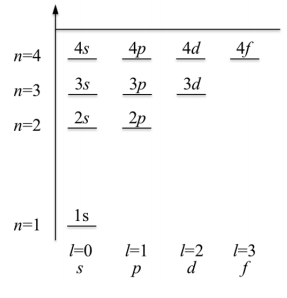
\includegraphics[width=0.3\textwidth]{figures/hyd}
			\caption{The lower energy levels of hydrogen. The degeneracy of $2s$ and $2p$ is evident.}
			\label{fig:hyd}
		\end{figure}
		
		\item \emph{$\braket{j=\frac{9}{2},m=\frac{7}{2},l=4|L_z|j=\frac{9}{2},m=\frac{7}{2},l=4}$ for an electron in a central force field.} \newline
		
		The above is not directly evaluate-able since $\ket{j,l,m}$ is not an eigenstate of $L_z$. Instead I use that
		\begin{equation}
			J_z=J_{1z}+J_{2z}=L_z+S_z.
		\end{equation} 
		In combination with
		\begin{equation}
			J_z\ket{j,l,m}=m\hbar\ket{j,l,m},
		\end{equation} 
		\begin{equation}
			\braket{j,m,l|S_z|j,m,l}|_{j=l\pm\frac{1}{2},m}=\pm\frac{m\hbar}{2l+1},
		\end{equation} 
		where I took the last identity from \citet{Sakurai}[p.338]. The result
		\begin{equation}
			\braket{j,m,l|L_z|j,m,l}=\frac{7}{2}\hbar-\frac{7\hbar}{2(24+1)}=\frac{28}{9}\hbar.
		\end{equation} 
		
		\item \emph{$\braket{singlet,m_s=0|S_z^{(e^-)}-S_z^{(e^+)}|triplet,m_s=0}$ for an $s$-state positronium.} \newline
		
		I use the definitions of the singlet and triplet states. The triplet state
		\begin{equation}
			\vec{S}^2: \quad\lambda_4^{(j=1,m=0)}=\frac{\hbar^2}{2}, \qquad \ket{\lambda_4}=\begin{bmatrix}
				\braket{+,+|\lambda_4} \\
				\braket{+,-|\lambda_4} \\
				\braket{-,+|\lambda_4} \\
				\braket{-,-|\lambda_4} \\
			\end{bmatrix}=\begin{bmatrix}
				0 \\
				1 \\
				1 \\
				0 \\
			\end{bmatrix}.
		\end{equation} 
		The above is also an eigenvector of $S_z$ since $[S_z,\vec{S}^2]=0$. Reformulated in a normalized way
		\begin{equation}
			\ket{j=1,m_s=0}=\frac{1}{\sqrt{2}}\bigg(\ket{+,-}+\ket{-,+}\bigg).
		\end{equation} 
		The singlet state
		\begin{equation}
			\vec{S}^2: \quad\lambda_1^{(j=0,m=0)}=0, \qquad \ket{\lambda_1}=\begin{bmatrix}
				\braket{+,+|\lambda_1} \\
				\braket{+,-|\lambda_1} \\
				\braket{-,+|\lambda_1} \\
				\braket{-,-|\lambda_1} \\
			\end{bmatrix}=\begin{bmatrix}
				0 \\
				1 \\
				-1 \\
				0 \\
			\end{bmatrix}.
		\end{equation} 
		Reformulated in a normalized way
		\begin{equation}
			\ket{j=0,m_s=0}=\frac{1}{\sqrt{2}}\bigg(\ket{+,-}-\ket{-,+}\bigg),
		\end{equation} 
		with the singlet and triplet states expressed in terms of the electron states I can now evaluate the matrix element. I let the operators act on the triplet state
		\begin{equation}
			\begin{split}
				\bigg(S_z^{(e^-)}-S_z^{(e^+)}\bigg)\ket{j=1,m_s=0}&=\bigg(S_z^{(e^-)}-S_z^{(e^+)}\bigg)\frac{1}{\sqrt{2}}\bigg(\ket{+,-}+\ket{-,+}\bigg)\\
				&=\frac{1}{\sqrt{2}}\bigg(\frac{\hbar}{2}+\frac{\hbar}{2}\bigg)\ket{+,-}+\frac{1}{\sqrt{2}}\bigg(-\frac{\hbar}{2}-\frac{\hbar}{2}\bigg)\ket{-,+}\\
				&=\frac{\hbar}{\sqrt{2}}\bigg(\ket{+,-}-\ket{-,+}\bigg)\\
				&=\hbar\ket{j=0,m_s=0}.
			\end{split}
		\end{equation} 
		So, the matrix element is found to be
		\begin{equation}
			\begin{split}
				\hbar&	\braket{j=0,m_s=0|S_z^{(e^-)}-S_z^{(e^+)}|j=1,m_s=0},\\
				&\hbar\braket{j=0,m_s=0|j=0,m_s=0}.
			\end{split}
		\end{equation} 
		
		\item \emph{$\braket{\vec{S}_{1}\cdot\vec{S}_{2}}$ for the ground state of a hydrogen molecule ($H_2$).} \newline
		
		I use that
		\begin{equation}
			\vec{S}_{1}\cdot\vec{S}_{2}=\frac{1}{2}(\vec{S}^2-\vec{S}_1^2-\vec{S}_2^2).
		\end{equation} 
		I take the lowest state to be a spin singlet with $m_s=0$. Thereby $\braket{\vec{S}}=0$ and $\braket{\vec{S}_1^2}=\braket{\vec{S}_2^2}=\frac{1}{2}(\frac{1}{2}+1)\hbar^2=\frac{3}{4}\hbar^2$. Thereby
		\begin{equation}
			\braket{\vec{S}_{1}\cdot\vec{S}_{2}}=\frac{1}{2}(\vec{S}^2-\vec{S}_1^2-\vec{S}_2^2)=\frac{1}{2}(0-\frac{3}{4}\hbar^2-\frac{3}{4}\hbar^2)=-\frac{3}{4}\hbar^2.
		\end{equation} 
	\end{enumerate}
\end{example}

\begin{example}
	\index{TIPT, uniform electric field}
	\index{Hydrogen}
	\emph{A one-electron atom whose GS is non-degenerate is placed in a uniform electric field i the $z$-direction. Obtain an approximate expression for the induced electric dipole moment of the GS by considering the expectation value of $ez$ with respect to the perturbed-state vector computed to first order. Show that the same expression can also be found from the energy shift of the GS computed to second order. Ignore spin.}\newline
	
	In this exercise the GS of a hydrogen-like atom is considered. That is the state $\ket{n,l,m}=\ket{1,0,0}$. Because the electric field is uniform, and in the $z$-direction, the perturbative Hamiltonian is given by
	\begin{equation}
		H'=-ez|\vec{E}|.
	\end{equation} 
	Since the GS is non-degenerate the state vector to first order is given by equation \eqref{correction state}
	\begin{equation}
		\ket{1,0,0}\simeq\ket{(1,0,0)^0}+\sum_{k\neq (1,0,0)^0}\frac{\braket{k^0|H'|(1,0,0)^0}}{E_{(1,0,0)^0}^{(0)}-E_{k}^{(0)}}\ket{k^0}.
	\end{equation} 
	So, the expectation value
	\begin{equation}
		\begin{split}
			\braket{H'}_{1,0,0}&=-e|\vec{E}|\bra{1,0,0}z\ket{1,0,0}\\
			&\simeq-e|\vec{E}|\bigg(-e|\vec{E}|\sum_{k\neq (1,0,0)^0}\frac{\braket{(1,0,0)^0|z|k^0}}{E_{(1,0,0)^0}^{(0)}-E_{k}^{(0)}}\bra{k^0}+\bra{(1,0,0)^0}\bigg)\\
			&\qquad\cdot z\bigg(\ket{(1,0,0)^0}-e|\vec{E}|\sum_{k\neq (1,0,0)^0}\frac{\braket{k^0|z|(1,0,0)^0}}{E_{(1,0,0)^0}^{(0)}-E_{k}^{(0)}}\ket{k^0}\bigg).
		\end{split}
	\end{equation} 	
	To evaluate this I use that $\braket{n',l',m'|z|n,l,m}=0$ unless $l'=l\pm1$ and $m=m'$. So, the element $\braket{(1,0,0)^0|z|(1,0,0)^0}=0$. So, the remainder
	\begin{equation}
		\begin{split}
			\braket{H'}_{1,0,0}&\simeq-e|\vec{E}|\bigg(-2e|\vec{E}|\sum_{k\neq (1,0,0)^0}\frac{|\braket{(1,0,0)^0|z|k^0}|^2}{E_{(1,0,0)^0}^{(0)}-E_{k}^{(0)}}\\
			&+e^2|\vec{E}|^2\sum_{k'\neq (1,0,0)^0}\sum_{k\neq (1,0,0)^0}\frac{\braket{k^0|z|(1,0,0)^0}}{E_{(1,0,0)^0}^{(0)}-E_{k}^{(0)}}\frac{\braket{(1,0,0)^0|z|k'^0}}{E_{(1,0,0)^0}^{(0)}-E_{k'}^{(0)}}\bra{k'^0}z\ket{k^0}\bigg).
		\end{split}
	\end{equation} 
	The last term vanishes since $0\neq \braket{k^0|z|(1,0,0)^0}$ if $k=n,1,0$ and likewise for $\braket{(1,0,0)^0|z|k'^0}$. However, $\bra{k'^0}z\ket{k^0}=0$ in these cases. Therefore
	\begin{equation}
		\braket{H'}_{1,0,0}\simeq 2e^2|\vec{E}|^2\sum_{k\neq (1,0,0)^0}\frac{|\braket{(1,0,0)^0|z|k^0}|^2}{E_{(1,0,0)^0}^{(0)}-E_{k}^{(0)}}.
	\end{equation} 
\end{example}

\begin{example}
	\index{TIPT, two-state system}
	\emph{The Hamiltonian for a two-state system can be written as}
	\begin{equation}
		H=H_0+H'\doteq\begin{bmatrix}
			E_1^{(0)} & 0 \\
			0 & E_2^{(0)}\\
		\end{bmatrix}+\lambda\begin{bmatrix}
			0 &  \Delta \\
			\Delta & 0\\
		\end{bmatrix}=\begin{bmatrix}
			E_1^{(0)} & \lambda \Delta \\
			\lambda \Delta & E_2^{(0)}\\
		\end{bmatrix}.
	\end{equation} 
	\emph{The energy eigenfunctions for the unperturbed problems ($\lambda=0$) are given by}
	\begin{equation}
		\ket{\phi_1^{(0)}}=\begin{bmatrix}
			1 \\
			0 \\
		\end{bmatrix} \quad \mbox{,} \quad \ket{\phi_2^{(0)}}=\begin{bmatrix}
			0 \\
			1 \\
		\end{bmatrix}.
	\end{equation} 
	
	\begin{enumerate}
		\item \emph{Solve this problem exactly to find the energy eigenvectors $\ket{E_{1,2}}$ and the energy eigenvalues $E_{1,2}$.}\newline
		
		The problem can be set up as a matrix equation on the form
		\begin{equation}
			H\vec{x}=E\vec{x}.
			\label{eq24}
		\end{equation} 
		Cf. Cramers rule (equation \eqref{cramer1}) this only has non-trivial solutions when
		\begin{equation}
			det(H-EI)=0.
		\end{equation} 
		From this I find the eigenvalues to be
		\begin{equation}
			E_{1,2}=\frac{E_1^{(0)}+E_2^{(0)}\mp\sqrt{(E_2^{(0)}-E_1^{(0)})^2+4\lambda^2\Delta^2}}{2}.
			\label{eq26}
		\end{equation} 
		By insertion of the eigenvalues into equation \eqref{eq24} the components of the eigenvectors can be found. This will result in two non-independent equations, and so one of the coefficients can be chosen to be 1 in order to determine the other. The unnormalized eigenvectors are therefore
		\begin{equation}
			\ket{E_{1}}=\begin{bmatrix}
				1 \\
				\frac{E_{1}-E_1^{(0)}}{\lambda\Delta} \\
			\end{bmatrix} \quad \mbox{;}\quad \ket{E_{2}}=\begin{bmatrix}
				\frac{E_{2}-E_2^{(0)}}{\lambda\Delta} \\
				1 \\
			\end{bmatrix}.
			\label{eq27}
		\end{equation} 
		The reason for the odd way to list the eigenvectors is to compare with the results from perturbation theory easily.\newline
		
		\item \emph{Assuming that $\lambda |\Delta|\ll |E_1^{(0)}-E_2^{(2)}|$, solve the same problem using time-independent perturbation theory up to first order in the energy eigenfunctions and up to second order in the energy eigenvalues. Compare with the exact results.}\newline
		
		From equation \eqref{correction energy}
		\begin{equation}
			\Delta E_n= \braket{n^0|H'|n^0}+\sum_{k\neq n}\frac{|\braket{k^0|H'|n^0}|^2}{E_n^0-E_k^0}+...,
		\end{equation} 
		where $\braket{n^0|H'|n^0}$ is the diagonal elements of the \emph{potential} matrix given by
		\begin{equation}
			H'\doteq\begin{bmatrix}
				0 & \lambda \Delta \\
				\lambda \Delta & 0\\
			\end{bmatrix}.
		\end{equation} 
		Hence the diagonal elements are zero, and so the first order correction to the energy (for both energy eigenvalues) is zero. For the second order correction
		\begin{equation}
			\begin{split}
				&\Delta E_1=\lambda \braket{1^0|H'|1^0}+\lambda^2\sum_{k\neq 1}\frac{|\braket{k^0|H'|1^0}|^2}{E_1^0-E_k^0}+...\\
				&\qquad=\lambda^2\frac{|\Delta|^2}{E_1^{(0)}-E_2^{(0)}},\\
				&\Delta E_2= \braket{2^0|H'|2^0}+\sum_{k\neq 1}\frac{|\braket{k^0|H'|2^0}|^2}{E_2^0-E_k^0}+...\\
				&\qquad=\lambda^2\frac{|\Delta|^2}{E_2^{(0)}-E_1^{(0)}}+....
			\end{split}
		\end{equation} 
		To compare with the exact result I consider $E_1$ as an example. I can rewrite it as\footnote{where I use $\lambda |\Delta|\ll |E_1^{(0)}-E_2^{(2)}|$ to Taylor expand the square root to second order; $\sqrt{1+x}=1+\frac{x}{2}+...$}
		\begin{equation}
			\begin{split}
				E_{1}&=\frac{E_1^{(0)}+E_2^{(0)}}{2}+\frac{E_2^{(0)}-E_1^{(0)}}{2}\sqrt{1+\frac{4\lambda^2\Delta^2}{(E_2^{(0)}-E_1^{(0)})^2}}\\
				&\simeq \frac{E_1^{(0)}+E_2^{(0)}}{2}+\frac{E_2^{(0)}-E_1^{(0)}}{2}\bigg(1+\frac{2\lambda^2\Delta^2}{(E_2^{(0)}-E_1^{(0)})^2}\bigg)\\
				&=E_1^{(0)}+\frac{\lambda^2\Delta^2}{E_1^{(0)}-E_2^{(0)}},
			\end{split}
		\end{equation} 
		which is the same as the exact case\footnote{A completely analogous procedure can be performed for $E_2$.}. For the eigenstates
		\begin{equation}
			\begin{split}
				&\ket{E_1}=\ket{E_1^{(0)}}+\lambda\sum_{k\neq 1}^{}\frac{\braket{k'^0|H'|E_1^{(0)}}}{E_1^{(0)}-E_{k'}^{(0)}}\ket{k^0}+\dots\\
				&\qquad=\ket{E_1^{(0)}}+\frac{\lambda\Delta}{E_1^{(0)}-E_{2}^{(0)}}\ket{E_2^{(0)}}+\dots,\\
				&\ket{E_2}=\ket{E_2^{(0)}}+\lambda\sum_{k\neq 1}^{}\frac{\braket{k'^0|H'|E_2^{(0)}}}{E_2^{(0)}-E_{k'}^{(0)}}\ket{k^0}+\dots\\
				&\qquad=\ket{E_2^{(0)}}+\frac{\lambda\Delta}{E_2^{(0)}-E_{1}^{(0)}}\ket{E_1^{(0)}}+\dots.
			\end{split}
			\label{eq25}
		\end{equation} 
		Inserting the eigenvalues in the exact results and Taylor expanding the square roots to second order will reveal the eigenvectors above found from perturbation theory
		\begin{equation}
			\begin{split}
				\ket{E_{1}}&\doteq\begin{bmatrix}
					1 \\
					\frac{E_{1}-E_1^{(0)}}{\lambda\Delta} \\
				\end{bmatrix}\\
				&=\begin{bmatrix}
					1 \\
					\frac{1}{\lambda\Delta}\bigg(\frac{E_1^{(0)}+E_2^{(0)}}{2}-\frac{(E_2^{(0)}-E_1^{(0)})}{2}\sqrt{1+\frac{4\lambda^2\Delta^2}{(E_2^{(0)}-E_1^{(0)})^2}}-E_1^{(0)}\bigg) \\
				\end{bmatrix}\\
				&\simeq\begin{bmatrix}
					1 \\
					\frac{1}{\lambda\Delta}\bigg(\frac{E_1^{(0)}+E_2^{(0)}}{2}-\frac{E_2^{(0)}-E_1^{(0)}}{2}(1+\frac{2\lambda^2\Delta^2}{(E_2^{(0)}-E_1^{(0)})^2})-E_1^{(0)}\bigg) \\
				\end{bmatrix}\\
				&=\begin{bmatrix}
					1 \\
					-\frac{1}{\lambda\Delta}\frac{E_2^{(0)}-E_1^{(0)}}{2}\frac{2\lambda^2\Delta^2}{(E_2^{(0)}-E_1^{(0)})^2} \\
				\end{bmatrix}=\begin{bmatrix}
					1 \\
					\frac{\lambda\Delta}{E_1^{(0)}-E_2^{(0)}} \\
				\end{bmatrix},
			\end{split}
		\end{equation} 
		which is identical to equation \eqref{eq25}.\newline
		
		\item \emph{Suppose the two unperturbed energy levels are "almost degenerate", i.e. $\lambda |\Delta|\gg |E_1^{(0)}-E_2^{(2)}|$. Show that the exact results obtained earlier closely resemble what you would expect by applying degenerate perturbation theory to this problem with $E_1^{(0)}=E_2^{(0)}=E^{(0)}$.}\newline
		
		In this case the Hamiltonian will be on the form
		\begin{equation}
			\begin{split}
				H&=H_0+H'\\
				&\doteq E^{(0)}\begin{bmatrix}
					1 & 0 \\
					0 & 1\\
				\end{bmatrix}+\lambda \Delta\begin{bmatrix}
					0 & 1 \\
					1 & 0\\
				\end{bmatrix}.
			\end{split}
		\end{equation} 
		I diagonalize $\lambda H'$. The eigenvalues are the first order correction to the energy whereas the eigenvectors are the eigenvectors of the energy levels. I find
		\begin{equation}
			E_1=E^{(0)}+\lambda\Delta \quad \mbox{and} \quad E_2=E^{(0)}-\lambda\Delta,
		\end{equation} 
		\begin{equation}
			\ket{E_1}=\begin{bmatrix}
				1 \\
				1 \\
			\end{bmatrix} \quad \mbox{and} \quad \ket{E_2}=\begin{bmatrix}
				-1 \\
				1 \\
			\end{bmatrix}.
		\end{equation} 
		Letting $E_1^{(0)}=E_2^{(0)}=E^{(0)}$ in equation \eqref{eq26} results in $E_i=E^{(0)}\pm\lambda\Delta$ just as above. Using $E_i=E^{(0)}\pm\lambda\Delta$ in equation \eqref{eq27} results in $\ket{E_i}=\begin{bmatrix}
			\pm1 \\
			1 \\
		\end{bmatrix}$ - just as above. Therefore, in the limit of almost degenerate energy levels, the exact method and the degenerate perturbation theory reveals the same result. 
		
	\end{enumerate}
\end{example}

\begin{example}
	\label{electric dipole}
	To illustrate the calculations required, I analyze the semi classical case of an electric dipole. I take $H'(t)$ to be on the form
	\begin{equation}
		H'(t)=-\vec{\mu}\cdot\vec{E}_0cos(\omega t),
		\label{semi clas}
	\end{equation} 
	where $\vec{E}_0$ is the magnitude of the electrical field, and unrelated to the energy, $E_n$. By using equation \eqref{semi clas} in \eqref{coef} I find the squared amplitude to be
	\begin{equation}
		|c^1_{b_0}(t_p)|^2=\bigg(\frac{E_0}{\hbar}\bigg)^2|\bra{b_0}\mu\ket{a_0}|^2\bigg|\int_{0}^{t_p}(-)e^{i\omega_{b_0a_0}t}cos(\omega t)dt\bigg|^2.
		\label{prob}
	\end{equation} 
	I define the integral as $I$ and evaluate it
	\begin{equation}
		\begin{split}
			I
			&=\int_{0}^{t_p}(-)e^{i\omega_{b_0a_0}t}cos(\omega t)dt\\
			&=\int_{0}^{t_p}(-)e^{i\omega_{b_0a_0}t}\bigg(\frac{e^{i\omega t}+e^{-i\omega t}}{2}\bigg)dt\\
			&=-\frac{1}{2}\int_{0}^{t_p}e^{i\omega_{b_0a_0}t}(e^{i\omega t}+e^{-i\omega t})dt\\
			&=-\frac{1}{2}\bigg(\int_{0}^{t_p}e^{i(\omega_{b_0a_0}+\omega)t}dt+\int_{0}^{t_p}e^{i(\omega_{b_0a_0}-\omega)t}dt\bigg)\\
			&=-\frac{1}{2}\bigg(\frac{e^{i(\omega_{b_0a_0}+\omega)t_p}-1}{i(\omega_{b_0a_0}+\omega)}+\frac{e^{i(\omega_{b_0a_0}-\omega)t_p}-1}{i(\omega_{b_0a_0}-\omega)}\bigg)\\
			&=\frac{1}{2i}\bigg(\frac{1-e^{i(\omega_{b_0a_0}+\omega)t_p}}{\omega_{b_0a_0}+\omega}+\frac{1-e^{i(\omega_{b_0a_0}-\omega)t_p}}{\omega_{b_0a_0}-\omega}\bigg).
		\end{split}
		\label{calc}
	\end{equation} 
	Using equation \eqref{calc} in \ref{prob} and letting the magnitude-operator absorb the imaginary unit, I find
	\begin{equation}
		|c^1_{b_0}(t_p)|^2=\bigg(\frac{E_0}{2\hbar}\bigg)^2|\bra{b_0}\mu\ket{a_0}|^2\bigg|\frac{1-e^{i(\omega_{b_0a_0}+\omega)t_p}}{\omega_{b_0a_0}+\omega}+\frac{1-e^{i(\omega_{b_0a_0}-\omega)t_p}}{\omega_{b_0a_0}-\omega}\bigg|^2.
	\end{equation} 
	To get considerable probability, the denominator needs to explode. This gives rise to the criterion for a large transition probability
	\begin{equation}
		\omega\simeq|\omega_{b_0a_0}|.
		\label{criterion}
	\end{equation} 
	Equation \eqref{criterion} causes the denominator in one of the fractions to "explode" -the other one does not explode, and can therefore be neglected. I find 
	\begin{equation}
		\begin{split}
			&\omega\simeq\omega_{b_0a_0} \quad |c^1_{b_0}(t_p)|^2\simeq\bigg(\frac{E_0}{2\hbar}\bigg)^2|\bra{b_0}\mu\ket{a_0}|^2\bigg|\frac{sin(\frac{\omega_{b_0a_0}-\omega}{2}t_p)}{\frac{\omega_{b_0a_0}-\omega}{2}}\bigg|^2,\\
			&\omega\simeq-\omega_{b_0a_0} \quad |c^1_{b_0}(t_p)|^2\simeq\bigg(\frac{E_0}{2\hbar}\bigg)^2|\bra{b_0}\mu\ket{a_0}|^2\bigg|\frac{sin(\frac{\omega_{b_0a_0}+\omega}{2}t_p)}{\frac{\omega_{b_0a_0}+\omega}{2}}\bigg|^2.
		\end{split}
		\label{trans1}
	\end{equation} 
	Using the definition of $\omega_{m_0n_0}=\frac{E_{m_0}-E_{n_0}}{\hbar}$
	\begin{equation}
		\begin{split}
			&\omega_{m_0n_0}>0:\quad\omega_{m_0n_0}=\frac{E_{b_0}-E_{a_0}}{\hbar}>0\\
			&\qquad \Rightarrow E_{b_0}>E_{a_0}\Rightarrow \mbox{Absorption of $1$ photon},\\
			&\omega_{m_0n_0}<0:\quad\omega_{m_0n_0}=\frac{E_{b_0}-E_{a_0}}{\hbar}<0\\
			&\qquad  \Rightarrow E_{b_0}<E_{a_0}\Rightarrow \mbox{Emission of $1$ photon}.
		\end{split}
	\end{equation} 
	In equation \eqref{trans1} $\omega_{b_0a_0}\pm\omega$ is raised to the second power and sine is an odd function to the second power\footnote{Meaning that $sin(-x)=-sin(x)$.}. This means that the probability for absorption and emission of $1$ photon is the same. The probability depends on the perturbation time and the frequency of the electromagnetic wave. The dependency of the perturbation time is shown in figure \ref{fig:pertub2}.
	\begin{figure}[ht]
		\captionsetup{width=1\textwidth}
		\centering
		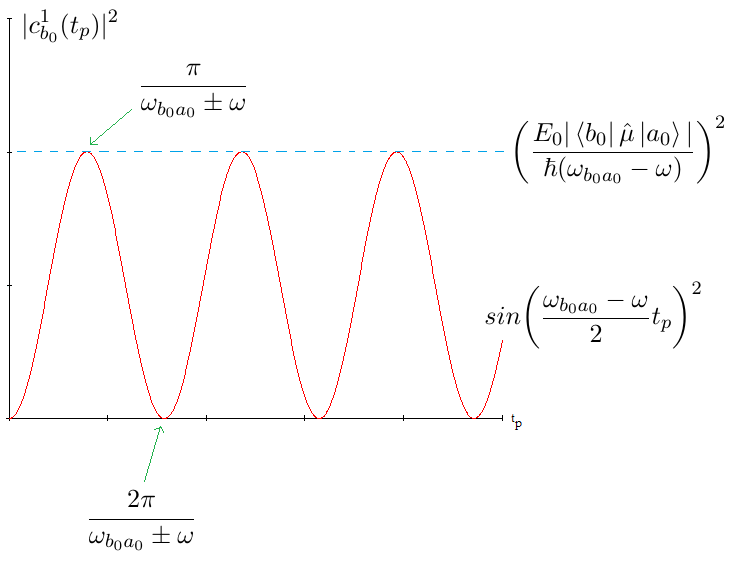
\includegraphics[width=0.6\textwidth]{figures/tipertub1}
		\caption{The transition probability as a function of perturbation time.}
		\label{fig:pertub2}
	\end{figure}
	As is evident from figure \ref{fig:pertub2}; the transition probability varies periodically with the perturbation time. To have greatest possibility of a transition, the perturbation time must be given by
	\begin{equation}
		t_p=\frac{(2k+1)\pi}{\omega_{b_0a_0}\pm\omega},
	\end{equation} 
	where $k=1,2,3,...$. The dependency of the transition probability on the angular frequency of the electromagnetic wave is shown in figure \ref{fig:pertub3}. Here equation \eqref{trans1} is rewritten to
	\begin{equation}
		\omega\simeq\omega_{b_0a_0} \quad |c^1_{b_0}(t_p)|^2\simeq\bigg(\frac{E_0|\bra{b_0}\mu\ket{a_0}|}{2\hbar}\bigg)^2t_p^2\bigg|sinc\bigg(\frac{\omega_{b_0a_0}-\omega}{2}t_p\bigg)\bigg|^2.
	\end{equation} 
	\begin{figure}[H]
		\captionsetup{width=1\textwidth}
		\centering
		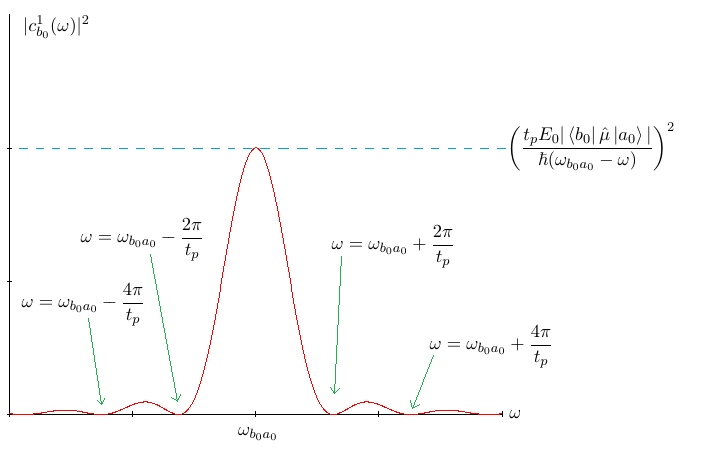
\includegraphics[width=0.6\textwidth]{figures/tipertub2}
		\caption{The transition probability as a function of the angular frequency of the electromagnetic wave.}
		\label{fig:pertub3}
	\end{figure}
	As is evident from figure \ref{fig:pertub3}; the transition probability peaks around $\omega_{b_0a_0}$. Thus, in order to maximize the transition probability, the time, $t_p$, and angular frequency, $\omega$, must have certain values.
\end{example}


\begin{example}
	\index{TDPT, SHO}
	\index{State vector in TDPT}
	\index{Expectation value in TDPT}
	\emph{Consider a one-dimensional simple harmonic oscillator whose classical angular frequency is $\omega_0$. For $t<0$ it is known to be in the ground state. For $t>0$ there is also a time-dependent potential given by}
	\begin{equation}
		H'(t)=F_0xcos(\omega t),
	\end{equation} 	
	\emph{where $F_0$ is constant in both space and time. Obtain an expression for the expectation value $\braket{x}$ as a function of time using time-dependent perturbation theory to lowest non-vanishing order. Is this procedure valid for $\omega\simeq \omega_0$?}\newline
	
	What is to be evaluated is
	\begin{equation}
		\braket{x}=\braket{0(t)|x|0(t)},
	\end{equation} 
	where
	\begin{equation}
		\ket{0(t)}=\sum_{n}c_n(t)e^{-i\frac{H_0t}{\hbar}}\ket{n}, \quad c_n(t)=c_n^{(0)}+c_n^{(1)}(t)+c_n^{(2)}(t)+\dots.
	\end{equation} 
	To first order; $c_0(t)=c_0^{(0)}$ since $\braket{0|x|0}$ from the first order term ($c_0^{(1)}$) is zero. For the first energy level;$c_1(t)=c_1^{(0)}+c_1^{(1)}(t)$ where $c_1^{0}=0$ cf. the initial condition that the state at $t=0$ is in the ground state. The rest of the coefficients, $c_n(t)$ ($n\geq2$) vanish since
	\begin{equation}
		\braket{n'|x|n}=\sqrt{\frac{\hbar}{2M\omega_0}}\bigg(\sqrt{n+1}\delta_{n',+1}+\sqrt{n}\delta_{n',n-1}\bigg).
		\label{hest}
	\end{equation} 
	Therefore
	\begin{equation}
		\ket{0(t)}=c_0^{(0)}e^{-\frac{1}{2}i\omega t}\ket{0}+c_1^{(1)}e^{-\frac{3}{2}i\omega t}\ket{1}.
	\end{equation} 
	Since at $t=0$ the state is in the ground state; $c_0^{0}\simeq1$. For the first excited state (from equation \eqref{coef})
	\begin{equation}
		\begin{split}
			c^1_{n}(t)&=\frac{1}{i\hbar}\int_{0}^{t}\bra{n}H'(t')\ket{0}e^{i\omega_{0}t'}dt'\\
			&=\frac{F_0\bra{n}x\ket{0}}{i\hbar}\int_{0}^{t}cos(\omega t')e^{i\omega_{0}t'}dt'\\
			&=\frac{F_0\bra{n}x\ket{0}}{i\hbar}\bigg(\int_{0}^{t}cos(\omega t')cos(\omega_0t')dt'+i\int_{0}^{t}cos(\omega t')sin(\omega_0t')dt'\bigg)\\
			&=\frac{F_0\bra{n}x\ket{0}}{2\hbar}\bigg(\frac{e^{-i(\omega-\omega_0)t}-1}{\omega-\omega_0}-\frac{e^{i(\omega+\omega_0)t}-1}{\omega+\omega_0}\bigg).\\
		\end{split}
	\end{equation} 
	So, to first order the expectation value can be written as
	\begin{equation}
		\begin{split}
			\braket{0(t)|x|0(t)}&=(\bra{1}e^{\frac{i3\hbar\omega_0t}{2}}c_1^{(1)*}+\bra{0}e^{\frac{i\hbar\omega_0t}{2}}c_0^{(0)})\\
			&\quad\cdot x(c_0^{(0)*}e^{\frac{-i\hbar\omega_0t}{2}}\ket{0}+c_1^{(1)}e^{\frac{-i3\hbar\omega_0t}{2}}\ket{1})\\
			&=\braket{1|x|0}e^{i\omega_0t}c_1^{(1)*}+\braket{0|x|1}e^{-i\omega_0t}c_1^{(1)},
		\end{split}
	\end{equation} 
	where equation \eqref{hest} has been used again to make the terms with $\braket{n|x|n}$ vanish. Thereby
	\begin{equation}
		\begin{split}
			\braket{x}&=\frac{F_0}{M}\frac{cos(\omega t)-cos(\omega_0t)}{\omega^2-\omega_0^2},
		\end{split}
	\end{equation} 
	where I have used that $\braket{1|x|0}=\sqrt{\frac{\hbar}{2M\omega_0}}$.
\end{example}

\begin{example}
	\index{TDPT, SHO}
	\index{Transition probability}
	\emph{A one-dimensional SHO is in its ground state for $t<0$. For $t\geq0$ it is subjected to a time.-dependent but spatially uniform force in the x-direction}
	\begin{equation}
		\vec{F}(t)=F_0e^{-\frac{t}{\tau}}\begin{bmatrix}
			1\\0\\0\\
		\end{bmatrix}.
	\end{equation} 
	
	\begin{enumerate}
		\item \emph{Using TDPT to first order, obtain the probability of finding the oscillator in its first excited state for $t>0$. Show that in the limit of $t\Rightarrow \infty$ the result is independent of time. Is this reasonable or surprising?} \newline
		
		First I convert the perturbative force into a perturbative potential which I can add to the Hamiltonian. I use that $\vec{F}=-\vec{\nabla}\cdot V(t)$. Hereby
		\begin{equation}
			V(t)=H'(t)=-F_0xe^{-\frac{t}{\tau}}.
		\end{equation} 
		The transition probability
		\begin{equation}
			P_{0\Rightarrow 1}(t)\simeq|c_1^{(1)}(t)|^2,
		\end{equation} 
		where
		\begin{equation}
			\begin{split}
				c_1^{(1)}(t)&=\frac{1}{i\hbar}\int_{0}^{t}\braket{1|H'(t')|0}e^{i\omega_{10}t'}dt'\\
				&=-\frac{\braket{1|x|0}F_0}{i\hbar}\int_{0}^{t}e^{t'(i\omega_{10}-\frac{1}{\tau})}dt'\\
				&=-\frac{\braket{1|x|0}F_0}{i\hbar}\frac{e^{t(i\omega_{10}-\frac{1}{\tau})}-1}{(i\omega_{10}-\frac{1}{\tau})}.\\
			\end{split}
		\end{equation} 
		By insertion
		\begin{equation}
			\begin{split}
				P_{0\Rightarrow 1}(t)&\simeq\bigg|-\frac{\braket{1|x|0}F_0}{i\hbar}\frac{e^{t(i\omega_{10}-\frac{1}{\tau})}-1}{(i\omega_{10}-\frac{1}{\tau})}\bigg|^2\\
				&=\frac{|\braket{1|x|0}|^2F_0^2}{\hbar^2}\bigg|\frac{e^{t(i\omega_{10}-\frac{1}{\tau})}-1}{(i\omega_{10}-\frac{1}{\tau})}\bigg|^2\\
				&=\frac{|\braket{1|x|0}|^2F_0^2}{\hbar^2}\frac{e^{t(i\omega_{10}-\frac{1}{\tau})}-1}{(i\omega_{10}-\frac{1}{\tau})}\frac{e^{t(-i\omega_{10}-\frac{1}{\tau})}-1}{(-i\omega_{10}-\frac{1}{\tau})}\\
				&=\frac{|\braket{1|x|0}|^2F_0^2}{\hbar^2}\frac{e^{-\frac{2t}{\tau}}-e^{-\frac{t}{\tau}}2cos(\omega_{10}t)+1}{\omega_{10}^2+\frac{1}{\tau^2}}.\\
			\end{split}
		\end{equation} 
		In the limit of $t\Rightarrow \infty$
		\begin{equation}
			\lim\limits_{t\Rightarrow\infty}(P_{0\Rightarrow 1}(t))\simeq\frac{|\braket{1|x|0}|^2F_0^2}{\hbar^2}\frac{1}{\omega_{10}^2+\frac{1}{\tau^2}}.
		\end{equation} 
		This makes sense since the perturbation will vanish in this limit. 
		
		\item \emph{Can higher states be the destination of the perturbation?}\newline
		
		Not to first order since $\braket{n'|x|0}=\sqrt{\frac{\hbar}{2M\omega}}\delta_{n',1}$. To second order (cf. equation \eqref{second order})
		\begin{equation}
			\begin{split}
				c^{(2)}_{b_0}(t)&=-\frac{1}{\hbar^2}\int_{0}^{t}\bra{b_0}H'(t'')\ket{1}e^{i\omega_{b_0,1}t''}\int_{0}^{t''}\bra{1}H'(t')\ket{0}e^{i\omega_{n_0,0}t'}dt'dt'',
				\\
			\end{split}
		\end{equation} 
		where I used that only $\bra{1}H'(t')\ket{0}\neq0$ which also requires $b_0=2$(!). This expression is in general non-zero, and so there is a finite transition probability to the second excited state.
	\end{enumerate}
\end{example}
\begin{example}
	\index{TDPT, SHO}
	\index{Transition probability}
	\emph{Consider a particle bound in a SHO potential. Initially ($t<0$) it is in the GS. At $t=0$ a perturbation is turned on. the perturbation is given by}
	\begin{equation}
		H'(x,t)=Ax^2e^{-\frac{t}{\tau}}.
	\end{equation} 
	\emph{calculate the probability that after a long time, $t\gg\tau$, the system will have made a transition to a given excited state. Consider all final states.}\newline
	
	Since $c_n^{(1)}\propto \braket{n^0|x^2|0^0}$ I consider these matrix elements. Cf. equation \eqref{shit}
	\begin{equation}
		\begin{split}
			\braket{n^0|x^2|0^0}&=\frac{\hbar}{2M\omega}\bigg(\braket{n^0|a^\dagger a|0^0}+\braket{n^0|a^\dagger a^\dagger|0^0}+\braket{n^0|aa^\dagger|0^0}+\braket{n^0|aa|0^0}\bigg)\\
			&=\frac{\hbar}{2M\omega}\bigg(\braket{n^0|a^\dagger a^\dagger|0^0}\delta_{n,2}+\braket{n^0|aa^\dagger|0^0}\delta_{n,0}\bigg).\\
		\end{split}
	\end{equation} 
	Here only the GS and the second excited state reveals any results. So, the relevant probability here is given by
	\begin{equation}
		P_{0\Rightarrow 2}(t)=|\braket{2|\alpha(t)}|^2=|c_2^{(1)}(t)|^2,
	\end{equation} 
	where
	\begin{equation}
		\begin{split}
			c_2^{(1)}(t)&=\frac{1}{i\hbar}\int_{0}^{t}\braket{2|H'(t')|0}e^{i\omega_{20}t'}dt'\\
			&=-\frac{\braket{2|x^2|0}A}{i\hbar}\int_{0}^{t}e^{t'(i\omega_{20}-\frac{1}{\tau})}dt'\\
			&=-\frac{\braket{2|x^2|0}A}{i\hbar}\frac{e^{t(i\omega_{20}-\frac{1}{\tau})}-1}{(i\omega_{20}-\frac{1}{\tau})}.\\
		\end{split}
	\end{equation} 
	By insertion
	\begin{equation}
		\begin{split}
			P_{0\Rightarrow 2}(t)&\simeq\bigg|-\frac{\braket{2|x^2|0}A}{i\hbar}\frac{e^{t(i\omega_{20}-\frac{1}{\tau})}-1}{(i\omega_{20}-\frac{1}{\tau})}\bigg|^2\\
			&=\frac{|\braket{2|x^2|0}|^2A^2}{\hbar^2}\bigg|\frac{e^{t(i\omega_{20}-\frac{1}{\tau})}-1}{(i\omega_{20}-\frac{1}{\tau})}\bigg|^2\\
			&=\frac{|\braket{2|x^2|0}|^2A^2}{\hbar^2}\frac{e^{t(i\omega_{20}-\frac{1}{\tau})}-1}{(i\omega_{20}-\frac{1}{\tau})}\frac{e^{t(-i\omega_{20}-\frac{1}{\tau})}-1}{(-i\omega_{20}-\frac{1}{\tau})}\\
			&=\frac{|\braket{2|x^2|0}|^2A^2}{\hbar^2}\frac{e^{-\frac{2t}{\tau}}-e^{-\frac{t}{\tau}}2cos(\omega_{20}t)+1}{\omega_{20}^2+\frac{1}{\tau^2}}.\\
		\end{split}
	\end{equation} 
	In the limit of $t\Rightarrow \infty$
	\begin{equation}
		\lim\limits_{t\Rightarrow\infty}(P_{0\Rightarrow 2}(t))\simeq\frac{|\braket{2|x^2|0}|^2A^2}{\hbar^2}\frac{1}{\omega_{20}^2+\frac{1}{\tau^2}}.
	\end{equation} 
	This makes sense since the perturbation will vanish in this limit.
\end{example}


\begin{example}
	\index{TDPT, two-state system}
	\emph{The unperturbed Hamiltonian of a two-state system is represented by}
	\begin{equation}
		H_0\doteq\begin{bmatrix}
			E_1^{(0)} & 0\\
			0 & E_2^{(0)} \\ 
		\end{bmatrix}.
	\end{equation} 
	\emph{The two state system is perturbed by}
	\begin{equation}
		H'(t)\doteq\begin{bmatrix}
			0 & \lambda cos(\omega t)\\
			\lambda cos(\omega t) & 0 \\ 
		\end{bmatrix},
	\end{equation} 
	\emph{where $\lambda$ is real.} \newline
	
	\begin{enumerate}
		\item \emph{At $t=0$ the system in known to be in the first state, represented by}
		\begin{equation}
			\ket{1}=\begin{bmatrix}
				1\\
				0 \\ 
			\end{bmatrix}.
		\end{equation} 
		\emph{Using TDPT and assuming that $E_1^{(0)}-E_2^{(0)}$ is not close to $\pm \hbar \omega$, derive an expression for the probability that the system is found in the second state represented by}
		\begin{equation}
			\ket{2}=\begin{bmatrix}
				0\\
				1 \\ 
			\end{bmatrix}
		\end{equation} 
		\emph{as a function of time.}\newline
		
		I use that
		\begin{equation}
			P_{1\Rightarrow 2}(t)=|\braket{2|\alpha(t)}|^2,
		\end{equation} 		
		where $\ket{\alpha(t)}$ is a general state vector described by
		\begin{equation}
			\ket{\alpha(t)}=c_1(t)e^{-\frac{iE_1^{(0)}t}{\hbar}}\ket{1}+c_2(t)e^{-\frac{iE_2^{(0)}t}{\hbar}}\ket{2}.
		\end{equation} 
		Since $\ket{1}$ and $\ket{2}$ are orthogonal the probability reduces to
		\begin{equation}
			P_{1\Rightarrow 2}(t)=|\braket{2|\alpha(t)}|^2=\big|c_2(t)e^{-\frac{iE_2^{(0)}t}{\hbar}}\big|^2=|c_2(t)|^2.
		\end{equation} 
		To first order
		\begin{equation}
			\begin{split}
				c_2^{(1)}(t)&=\frac{1}{i\hbar}\int_{0}^{t}\braket{2|H'(t')|1}e^{i\omega_{21}t'}dt'\\
				&=\frac{\lambda}{i\hbar}\int_{0}^{t}cos(\omega t)e^{i\omega_{21}t'}dt'.\\
			\end{split}
		\end{equation} 
		From this the probability can be found; use partial integration or see section \ref{electric dipole}.
		
	\end{enumerate}
\end{example}

\begin{example}
	\index{TDPT, two-state system}
	\emph{Consider a two-level system with $E_1<E_2$. There is a time-dependent potential that connects the two levels as follows}
	\begin{equation}
		H'\doteq\begin{bmatrix}
			0 & \gamma e^{i\omega t} \\
			\gamma e^{-i\omega t} & 0\\
		\end{bmatrix},
	\end{equation} 	
	\emph{where $\gamma$ is a real constant. At $t=0$, it is known that only the lower level is populated (i.e. $c_1(0)=1$, $c_2(0)=0$).}\newline
	
	\begin{enumerate}
		\item \emph{Find $|c_1(t)|^2$ and $|c_2(t)|^2$ for $t>0$ by exactly solving the coupled differential equation}
		\begin{equation}
			i\hbar\frac{\partial c_k}{\partial t}=\sum_{n=1}^{2}\braket{k|H'(t)|n}e^{i\omega_{kn}t}c_n,
		\end{equation}		
		\emph{where $k=1,2$.}\newline
		
		I use that
		\begin{equation}
			i\hbar\frac{\partial c_1}{\partial t}=\gamma e^{i(\omega+\omega_{12}) t}c_2,
		\end{equation} 
		\begin{equation}
			i\hbar\frac{\partial c_2}{\partial t}=\gamma e^{i(\omega_{21}-\omega) t}c_1.
			\label{eq28}
		\end{equation} 
		I isolate $c_1$ from the second equation, differentiate it and insert it in the first equation. I find
		\begin{equation}
			\frac{\partial^2 c_2}{\partial t^2}+i(\omega-\omega_{21}))\frac{\partial c_2}{\partial t}+\frac{\gamma^2}{\hbar^2} e^{i(\omega_{12}+\omega_{21})t}c_2=0.
		\end{equation} 
		Using now that $\omega_{12}=-\omega_{21}$
		\begin{equation}
			\frac{\partial^2 c_2}{\partial t^2}+i(\omega-\omega_{21})\frac{\partial c_2}{\partial t}+\frac{\gamma^2}{\hbar^2}c_2=0.
		\end{equation} 
		Using the auxiliary equation I identify
		\begin{equation}
			\begin{split}
				&a=1,\\
				&b=i(\omega-\omega_{21}),\\
				&c=\frac{\gamma^2}{\hbar^2}.\\
			\end{split}
		\end{equation} 
		Using then that
		\begin{equation}
			D=b^2-4ac=-(\omega-\omega_{21})^2-\frac{4\gamma^2}{\hbar^2}<0,
		\end{equation} 
		the solution is on the form
		\begin{equation}
			c_2(t)=Acos(\omega_0t)+Bsin(\omega_0t),
		\end{equation} 
		where from $c_2(0)=0\Rightarrow A=0$, and $\omega_0$ is found from
		\begin{equation}
			r=\frac{-b\pm\sqrt{b^2-4ac}}{2a}=k\pm i\omega_0.
		\end{equation} 
		Evaluating $r$
		\begin{equation}
			\begin{split}
				r&=0\pm\frac{i}{2}\bigg(\sqrt{(\omega-\omega_{21})^2+\frac{4\gamma^2}{\hbar^2}}-(\omega-\omega_{21})\bigg)\\
				&\Rightarrow \omega_0=\frac{1}{2}\bigg(\sqrt{(\omega-\omega_{21})^2+\frac{4\gamma^2}{\hbar^2}}-(\omega-\omega_{21})\bigg).
			\end{split}
		\end{equation} 
		So
		\begin{equation}
			c_2(t)=Bsin(\omega_0t).
		\end{equation} 
		From using this in equation \eqref{eq28}
		\begin{equation}
			c_1(t)=\frac{i\hbar}{\gamma e^{i(\omega_{21}-\omega)t}}\frac{\partial c_2(t)}{\partial t}=\frac{iB\omega_0\hbar}{\gamma}e^{i(\omega-\omega_{21})t}cos(\omega_0t),
		\end{equation} 
		since $c_1(0)=1\Rightarrow B=-\frac{i\gamma}{\omega_0\hbar}$. So
		\begin{equation}
			\begin{split}
				&c_1(t)=e^{-i(\omega+\omega_{21})t}cos(\omega_0t),\\
				&c_2(t)=-\frac{i\gamma}{\omega_0\hbar}sin(\omega_0t).\\
			\end{split}
		\end{equation} 
		The probabilities
		\begin{equation}
			\begin{split}
				&|c_1(t)|^2=cos(\omega_0t)^2,\\
				&|c_2(t)|^2=\frac{\gamma^2sin(\omega_0t)^2}{\hbar^2\omega_0^2}.\\
			\end{split}
		\end{equation} 
		From which certain restrictions on $\gamma$ can be made.
		
		\item \emph{Do the same problem using time-dependent perturbation theory to lowest non-vanishing order. Compare the two approaches for small values of $\gamma$. Treat the following two cases separately: (i) $\omega$ very different from $\omega_{21}$ and (ii) $\omega$ close to $\omega_{21}$.}\newline
		
		From equation \eqref{coef}
		\begin{equation}
			\begin{split}
				c^1_{2}(t)&=\frac{1}{i\hbar}\int_{0}^{t}\bra{2}H'(t')\ket{1}e^{i\omega_{21}t'}dt'\\
				&=\frac{\gamma}{i\hbar}\int_{0}^{t} e^{i(\omega_{21}-\omega )t'}dt'\\
				&=\frac{\gamma}{\hbar (\omega_{21}-\omega )}(1-e^{i(\omega_{21}-\omega )t}).\\
			\end{split}
		\end{equation} 
		The probability
		\begin{equation}
			\begin{split}
				|c^1_{2}(t)|^2&=\frac{\gamma^2}{\hbar^2 (\frac{\omega_{21}-\omega }{2})^2}sin\bigg(\frac{\omega_{21}-\omega}{2}t\bigg)^2.\\
			\end{split}
		\end{equation} 
		From the above $|c_2(t)|^2$ can be found from $|c_2(t)|^2=1-|c_2(t)|^2$. Comparing the perturbative result with the exact result it is clear that the condition is
		\begin{equation}
			\omega_0=\frac{1}{2}\bigg(\sqrt{(\omega-\omega_{21})^2+\frac{4\gamma^2}{\hbar^2}}-(\omega-\omega_{21})\bigg) \Rightarrow \frac{\omega_{21}-\omega}{2},
		\end{equation} 
		where the arrow indicates "should be equal to". This is satisfied only when
		\begin{equation}
			(\omega-\omega_{21})^2\gg\frac{4\gamma^2}{\hbar^2}.
		\end{equation} 
		In the case where $\omega\simeq\omega_{21}$ the exact and approximate probability reduces to
		\begin{equation}
			\omega\simeq\omega_{21}, \mbox{exact:} \qquad |c_2(t)|^2\simeq sin\bigg(\frac{\gamma}{\hbar}t\bigg)^2,
		\end{equation} 
		\begin{equation}
			\omega\simeq\omega_{21}, \mbox{approx:} \qquad |c^{(1)}_2(t)|^2\simeq \frac{\gamma^2t^2}{\hbar^2}.
		\end{equation} 
		As is apparent from above the approximate solution is not bound to below one, and as time goes it can go above 1 and become unphysical. The two are however equivalent at $t\sim 0$.\newline For $\omega$ very different from $\omega_{21}$ the relation $(\omega-\omega_{21})^2\gg\frac{4\gamma^2}{\hbar^2}$ is satisfied and the two results will be equal.
		
	\end{enumerate}
\end{example}

\begin{example}
	\index{Selection rules}
	\index{TDPT, hydrogen atom}
	\index{Transition probability}
	\index{First order TDPT}
	\emph{A hydrogen atom in its ground state [(n,l,m=(1,0,0))] is placed between the plates of a capacitor. A time-dependent but spatially uniform electric field (not potential!) is applied as follows}
	\begin{equation}
		\vec{E}=\begin{cases} 0 &\mbox{for} \quad t<0 \\ 
			\vec{E}_0e^{-\frac{t}{\tau}} & \mbox{for} \quad t\geq 0  \end{cases}. 
	\end{equation} 
	
	\emph{Using first-order time-dependent perturbation theory, compute the probability for the atom to be found at $t\gg \tau$ in each of the three $2p$ sates: $(n,l,m)=(2,1,\pm1 \mbox{or } 0)$. Repeat the problem for the 2s state: $(n,l,m)=(2,0,0)$. You need not attempts to evaluate radial integrals, but perform all other integrations (with respect to angles and time).}\newline
	
	Assuming the electric field is applied in the $z$-direction, the perturbative term added to the Hamiltonian is given from the linear Stark effect
	\begin{equation}
		H'(t)=-ez|\vec{E}_0|e^{-\frac{t}{\tau}}.
	\end{equation} 
	Thereby the first order correction
	\begin{equation}
		\begin{split}
			c^1_{f}(t)&=\frac{1}{i\hbar}\int_{0}^{t}\bra{f}H'(t')\ket{1,0,0}e^{i\omega_{0}t'}dt'\\
			&=\frac{-e|\vec{E}_0|}{i\hbar}\int_{0}^{t}\bra{f}z\ket{1,0,0}e^{(i\omega_{0}-\frac{1}{\tau})t'}dt',\\
		\end{split}
	\end{equation} 
	where $\ket{f}\in\{\ket{2,1,1}, \ket{2,1,-1}, \ket{2,1,0}\}$ for the $2p$ states. Cf. the arguments made in section \ref{sec:hydrogenmat}\footnote{Regarding the matrix element of angular momentum eigenstates with respect to $z$. Expressing $z$ as im terms of spherical tensors, and seeing that unless $m=m'\pm q$ the matrix element is zero. Now, since $T_{0}^{(1)}=z$ only $m=m'$ is non-zero.} the probability for the system to end up in $\ket{2,1,1}$ and $\ket{2,1,-1}$ is zero. Thereby on the case of $1s\Rightarrow 2p$ there is only one non-vanishing probability to end up in one of the given states. This is given as the following coefficient squared
	\begin{equation}
		\begin{split}
			c^1_{2,1,0}(t)&=\frac{-e|\vec{E}_0|}{i\hbar}\int_{0}^{t}\bra{2,1,0}z\ket{1,0,0}e^{(i\omega_{0}-\frac{1}{\tau})t'}dt'\\
			&=\frac{-e|\vec{E}_0|\braket{2,1,0|z|1,0,0}}{i\hbar}\int_{0}^{t}e^{(i\omega_{0}-\frac{1}{\tau})t'}dt'\\
			&=\frac{-e|\vec{E}_0|\braket{2,1,0|z|1,0,0}}{i\hbar(i\omega_{0}-\frac{1}{\tau})}\bigg(e^{(i\omega_{0}-\frac{1}{\tau})t}-1\bigg).
		\end{split}
	\end{equation} 
	So, the probability for a transition from $\ket{1,0,0}$ to $\ket{2,1,0}$ is given by
	\begin{equation}
		\begin{split}
			|c^1_{2,1,0}(t)|^2&=\frac{e^2|\vec{E}_0|^2|\braket{2,1,0|z|1,0,0}|^2}{\hbar^2\omega_{0}^2+\frac{\hbar^2}{\tau^2}}\bigg(e^{(i\omega_{0}-\frac{1}{\tau})t}-1\bigg)\bigg(e^{(-i\omega_{0}-\frac{1}{\tau})t}-1\bigg)\\
			&=\frac{e^2|\vec{E}_0|^2|\braket{2,1,0|z|1,0,0}|^2}{\hbar^2\omega_{0}^2+\frac{\hbar^2}{\tau^2}}\bigg(1+e^{-\frac{2t}{\tau}}-e^{-\frac{t}{\tau}}cos(\omega_0t)\bigg).\\
		\end{split}
	\end{equation} 
	In the limit of $t\gg\tau$ the exponential terms will go to zero. Therefore
	\begin{equation}
		\begin{split}
			t\gg\tau:\qquad|c^1_{2,1,0}(t)|^2\simeq=\frac{e^2|\vec{E}_0|^2|\braket{2,1,0|z|1,0,0}|^2}{\hbar^2\omega_{0}^2+\frac{\hbar^2}{\tau^2}}.\\
		\end{split}
	\end{equation} 
	The transition $\ket{1,0,0}\Rightarrow \ket{2,0,0}$ is also forbidden (probability is zero) since, cf.~\citep[p.322]{Sakurai}
	\begin{equation}
		\braket{n',l',m'|z|n,l,m}=0 \quad \mbox{unless} \begin{cases}
			l'=l\pm1 \\ m'=m
		\end{cases}.
	\end{equation} 
	The criterion $m=m'$ comes from the fact that $z$ can be written as a spherical tensor, $T_{0}^{(1)}=z$, and the matrix element of one such is zero unless $m=m'\pm q$ where $q=0$ in this case. The criterion $l'=l\pm1$ comes from parity. The above criterion are called \emph{selection rules}\index{Selection rules}. 
\end{example}

\begin{example}
	I consider a bumpy potential in the bottom of an infinitely deep potential well. The potential function is given by
	\begin{equation}
		V(x)=\begin{cases}
			&V(x) \qquad \mbox{for $0<x<a$} \\
			&\infty \qquad \quad \mbox{otherwise}
		\end{cases}.
	\end{equation} 
	
	The potential is shown in figure \ref{fig:wkb1}.
	\begin{figure}[H]
		\captionsetup{width=1\textwidth}
		\centering
		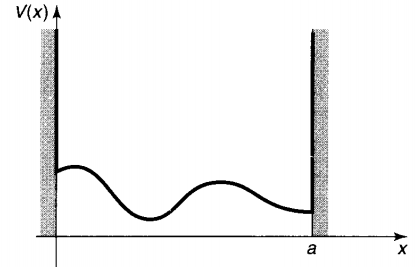
\includegraphics[width=0.4\textwidth]{figures/wkb1}
		\caption{The imagined potential in the bottom of an infinite well.}
		\label{fig:wkb1}
	\end{figure}
	
	I assume that $p(x)$ is real, the classical case, and thus $E>V(x)$ from equation \eqref{sch11}. From equation \eqref{sol} I find
	\begin{equation}
		\psi(x)\simeq\frac{1}{\sqrt{p(x)}}(C_+e^{i\phi(x)}+C_-e^{-i\phi(x)}),
		\label{sol4}
	\end{equation} 
	where
	\begin{equation}
		\phi(x)=\frac{1}{\hbar}\int_{0}^{x} p(x')dx'.
	\end{equation} 
	Using that $e^{\pm i x}=cos(x)\pm isin(x)$ I rewrite equation \eqref{sol4}
	\begin{equation}
		\psi(x)\simeq\frac{1}{\sqrt{p(x)}}((C_++C_-)cos(\phi(x))+(C_+-C_-)sin(\phi(x)).
		\label{sol5}
	\end{equation} 
	Since $\psi(x)\Rightarrow0$ at $x=0$ $C_++C_-=0$. Likewise, $\psi(x)\Rightarrow0$ at $x=a$, which results in $\phi(x)=n\pi$. Thus
	\begin{equation}
		\psi(x)\simeq\frac{1}{\sqrt{p(x)}}(C_+-C_-)sin(\phi(x)),
		\label{sol6}
	\end{equation} 
	where
	\begin{equation}
		\int_{0}^{a}p(x)dx=n\pi\hbar.
	\end{equation} 
	The quantization determines the approximate energy eigenvalues. They are determined by evaluating $p=\sqrt{2M(E-V(x))}$ and $\int_{0}^{a}p(x)dx=n\pi\hbar$ for $p(x)$ and equating the results. With $\phi(x)$ evaluated wave-function in equation \eqref{sol6} is also determined.
\end{example}

\begin{example}
	In this example I consider quantum tunneling, which corresponds to the non-classical case where $E<V$ and thereby $p(x)$ is imaginary. By setting $E<V$ I find from equation \eqref{sol}
	\begin{equation}
		\psi(x)\simeq\frac{C}{\sqrt{|p(x)|}}e^{\pm\frac{1}{\hbar}\int |p(x)|dx}.
		\label{sol7}
	\end{equation} 
	Quantum tunneling is non-classical because a particle of lower energy travels through a larger potential barrier. The probability of traveling through the barrier can be found by considering the wave function hitting the(a rectangular) barrier. I consider the scenario shown in figure \ref{fig:wkb2}.
	\begin{figure}[H]
		\captionsetup{width=1\textwidth}
		\centering
		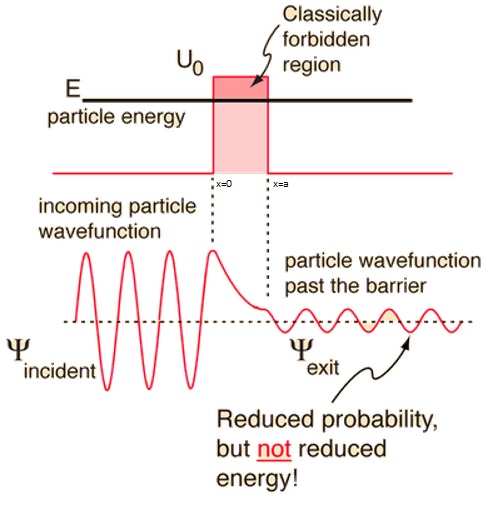
\includegraphics[width=0.5\textwidth]{figures/wkb2}
		\caption{Quantum tunneling.}
		\label{fig:wkb2}
	\end{figure}
	Analog to classical wave-physics, the involved waves will be an incident wave (I) a reflected wave(R) and a transmitted wave(T). I define $x=0$ where the wall starts, and $x=a$ where it ends. At $x<0$ the the incident and reflected wave is described by the wave function\footnote{The potential is constant, so the integral just evaluates to $x$.}
	\begin{equation}
		\psi_{x<0}(x)=Ie^{ik_1x}+Re^{-ik_1x},
	\end{equation} 
	where the subscript "$x<0$" denotes that this is the wave function for $x<0$, $I$ and $R$ are the amplitudes of the incident and reflected wave, respectively, and\footnote{At $x<0$ $V(x)=0$. I have used this in $p=\sqrt{2M(E-V(x))}$  along with $k=\frac{p}{\hbar}$.} $k_1=\frac{\sqrt{2ME}}{\hbar}$. I write the wave function in the tunneling region, $0<x<a$, as (with constant potential, $E_0$)
	\begin{equation}
		\psi_{0<x<a}(x)=C_1e^{ik_2x}+C_2e^{-ik_2x},
	\end{equation} 
	where $k_2=\frac{\sqrt{2M(E_0-E)}}{\hbar}$. I write the transmitted wave at $x>a$ as
	\begin{equation}
		\psi_{x>a}(x)=Te^{ik_1x}.
	\end{equation} 
	From my definitions the transmission probability is given by
	\begin{equation}
		P_{trans}=\frac{|T|^2}{|I|^2}.
	\end{equation} 
	I find $P_{trans}$ by evaluating the amplitudes $T$ and $I$ via imposing boundary conditions. I require continuity at the boundaries
	\begin{equation}
		\psi_{x<0}(0)=\psi_{0<x<a}(0),
	\end{equation} 
	\begin{equation}
		\frac{\partial \psi_{x<0}(0)}{\partial x}=\frac{\partial \psi_{0<x<a}(0)}{\partial x},
	\end{equation} 
	\begin{equation}
		\psi_{0<x<a}(a)=\psi_{x>0}(a),
	\end{equation} 
	\begin{equation}
		\frac{\partial \psi_{0<x<a}(a)}{\partial x}=\frac{\partial \psi_{x>0}(a)}{\partial x}.
	\end{equation} 
	From the BC I find
	\begin{equation}
		R=\frac{1}{2}\bigg(C_2(1-\frac{ik_2}{k_1})+C_1(1+\frac{ik_2}{k_1})\bigg),
	\end{equation} 
	\begin{equation}
		I=\frac{1}{2}\bigg(C_2(1+\frac{ik_2}{k_1})+C_1(1-\frac{ik_2}{k_1})\bigg),
	\end{equation} 
	\begin{equation}
		C_2=\frac{B_3}{2}(1-\frac{ik_1}{k_2})e^{-(ik_1+k_2)a},
	\end{equation} 
	\begin{equation}
		C_1=\frac{B_3}{2}(1+\frac{ik_1}{k_2})e^{(k_2-ik_1)a}.
	\end{equation} 
	Thus, I find the transmission probability ($P_{trans}$) as~\citep[p.340]{BR}
	\begin{equation}
		P_{trans}=\bigg|\frac{2k_1k_2e^{-k_1a}}{2k_1k_2cosh(k_2a)-i(k_1^2-k_2^2)sinh(k_2a)}\bigg|^2.
		\label{ptrans}
	\end{equation} 
	For large $k_2a$, which corresponds to small penetrations, I can make the small angle approximations
	\begin{equation}
		sinh(k_2a)\approx
		cosh(k_2a)\approx\frac{e^{k_2a}}{2}.
	\end{equation} 
	Thus, equation \eqref{ptrans} reduces to
	\begin{equation}
		P_{trans}\approx\bigg(\frac{4k_1k_2}{k_1^2+k_2^2}\bigg)^2e^{-2k_2a}.
		\label{ptrans2}
	\end{equation} 
	The first factor is down to reflection losses at the two boundaries ($x=0$ and $x=a$). The exponential describes the exponential decay of the amplitude of the wave function inside the barrier. The first factor varies slowly with energy and is therefore often neglected. Thus, the transmission probability is written as
	\begin{equation}
		P_{trans}\approx e^{-2k_2a}.
		\label{ptrans3}
	\end{equation} 
	Taking into account that the potential could be non-constant in the tunneling region, I find
	\begin{equation}
		P_{trans}\approx e^{-\frac{2}{\hbar}\int_{0}^{a}|p(x)|dx}=e^{-\frac{2}{\hbar}\int_{0}^{a}|\sqrt{2M(V(x)-E)}|dx},
		\label{ptrans4}
	\end{equation} 
	where $V(x)$ and $E$ has switched places because of the imaginary unit is "pulled out" and I consider the magnitude. From equation \eqref{ptrans4} it is clear that the incoming wave decays approximately exponentially inside the barrier, so the relationship between the incident and outgoing wave is the exponential decay. This squared gives the (approximate) transmission probability. The transmission probability is often used eg. in $\alpha$ particle decay or in nuclear fusion.
\end{example}
	
	\part{Relativistic Mechanics}
	\chapter*{Introduction}
		The subject of relativistic mechanics is the realm of classical fields in the relativistic limit. Classical because the theory describes macroscopic objects and fields because the laws of nature must be \emph{local}. The non-relativistic physical laws, of eg. Newton and Coulomb, employ "action at a distance". The principle of action at a distance approximates the speed of light to be infinite, and so information is mediated instantaneously between objects. This approximation is good when considering systems in the non-relativistic limit, but not in the relativistic limit. In the relativistic limit fields are needed to mediate the interactions, and besides that special relativity, or general relativity, is needed to describe the physics in a Lorentz covariant way. SR is closely related to group theory, and so the place to begin is really with an introduction to group theory ending with an introduction of the group used in special relativity; the Lorentz group. 
	
	\chapter{Group Theory and Special Relativity}
\label{chp:group theory}
Group theory concerns the classification of mathematical similarities between sets of elements and connects these to physical symmetries. 
\paragraph{Definition of a group: }
A set of elements, $a,b,c,...\in G$, is said to form a group if there, between two arbitrary elements of the group, exists a well defined product that satisfies:
\begin{enumerate}
	\item The product of two elements of the group is another element the group $a\cdot b=c$, $\forall a,b:\ni c:a,b,c\in G$.
	\item The group product between several elements is associative, i.e. $a\cdot(b\cdot c)=(a\cdot b)\cdot c$, $\forall a,b,c\in G$.
	\item The identity element exists within the group, i.e. $e\in G$. The identity is defined by the operation on other, generic elements via $a\cdot e=e\cdot a=a$, $\forall a\in G, e\in G$.
	\item There is an inverse to each group element, such that $a^{-1}\cdot a=a\cdot a^{-1}=e$, $\forall a\in G, e\in G$.
\end{enumerate}
\paragraph{An abelian group: }
A group is said to be abelian if the product of group elements is commutative, i.e. $a\cdot b=b\cdot a$, $\forall a,b\in G$.
\paragraph{Order of a group: }
The order of a group is the number of elements in the group.
\paragraph{Subgroup: }
If a subset, $H$, of a group, $G$, fulfill the requirements for a group, then the subset forms a subgroup.
\paragraph{Continuous group: }
If the group elements carry a label, which is a continuous parameter, the group is said to be continuous. A continuous group of special interest to physics is the Lie group\index{Lie group}. A Lie group is a group which is also a differentiable manifold\index{Manifold}. In mathematics, a manifold is a topological space that locally resembles Euclidean space near each point. This means that a geometrical structure can be associated with Lie groups and the group can be associated with such a structure in some abstract space. Further more, the elements of a Lie group must be parameterized smoothly and continuously.
\begin{example}
	\begin{enumerate}
		\item The general linear group, of dimension $n$, $GL(n)$, can be represented as the set of all invertible $n\times n$ matrices.
		\item The unitary group, of dimension $n$, $U(n)$, can be represented as the set of $n\times n$ unitary matrices. Ie. matrices satisfying $UU^\dagger=U^\dagger U=I$.
		\item The special unitary group, of dimension $n$, $SU(n)$, can be represented as the set of unitary matrices with unit determinant.
		\item The orthogonal group, of dimension $n$, $O(n)$, can be represented as the set of real, orthogonal matrices. Ie. matrices satisfying $M^T=M^{-1}$. The different groups are connected via the relation
		\begin{equation}
			SU(n)\wedge O(n)\in U(n)\in GL(n).
		\end{equation} 
		The relationship is also seen illustrated in figure \ref{fig:2}.
		\begin{figure}[h]
			\captionsetup{width=1\textwidth}
			\centering
			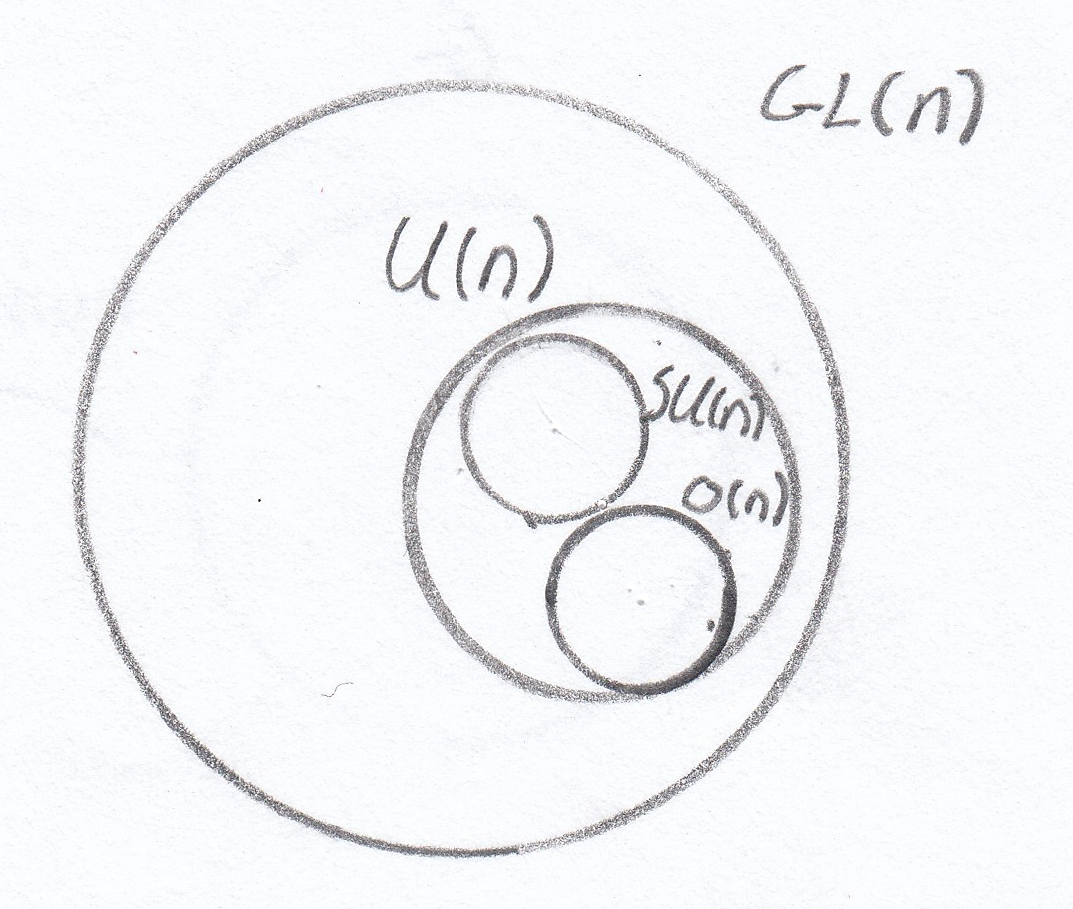
\includegraphics[width=0.4\textwidth]{figures//2}
			\caption{The relationship between the different groups mentioned above.}
			\label{fig:2}
		\end{figure}
	\end{enumerate}
\end{example}

\paragraph{Homomorphism: }
A homomorphism is a mapping between two groups, $G$ and $G'$, that conserve group multiplication. The map does not have to be one-to-one. An illustration of the mapping is seen in figure \ref{fig:3}.
\begin{figure}[h]
	\captionsetup{width=1\textwidth}
	\centering
	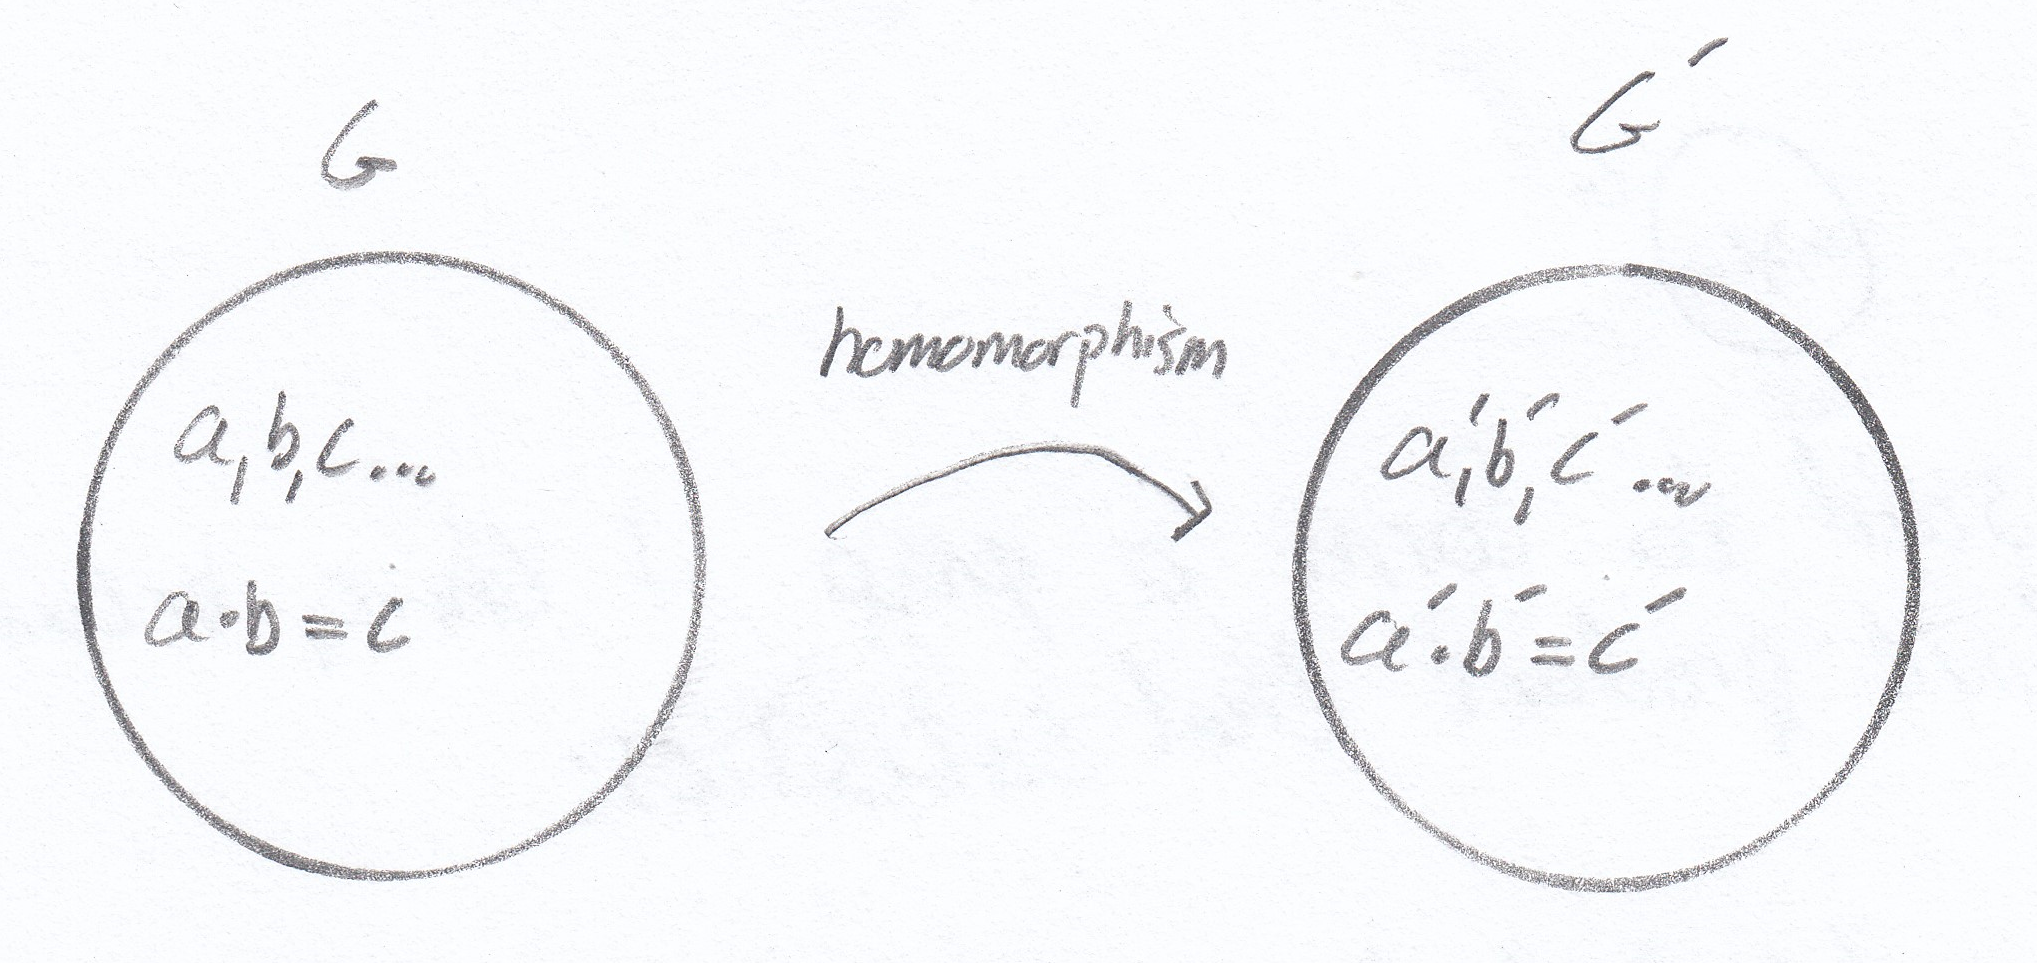
\includegraphics[width=0.5\textwidth]{figures//3}
	\caption{An illustration of a homomorphism between two groups.}
	\label{fig:3}
\end{figure}

\paragraph{Isomorphism: }
An isomorphism is a homomorphism between two groups, $G$ and $G'$, with a one-to-one correspondence. Hence, not only group multiplication is preserved, but also
\begin{equation}
	a \rightleftarrows a', \quad b \rightleftarrows b', \quad  c \rightleftarrows c',...
\end{equation}  
\paragraph{Conjugate elements of a group: }
Elements of a group, $G$, $a,b\in G$, is said to be conjugate to each other if there exist another element, $p\in G$, such that $b=pap^{-1}$.
\paragraph{Direct product group: }
Let $H_1$ and $H_2$ be subgroups of $G$ which satisfies:
\begin{enumerate}
	\item All elements of $H_1$ and $H_2$ commute, i.e. $h_1h_2=h_2h_1$, $\forall h\in H_1 \wedge h_2\in H_2$.
	\item All elements of $G$ can be described as the product of an element from $H_1$ and an element from $H_2$. Ie. $h_1h_2=g\in G, \forall g$. 
\end{enumerate}
In this case $G$ is said to be the direct product of $H_1$ and $H_2$. This is denoted by $G=H_1\otimes H_2$.
\paragraph{Group representation: }
If there is a homomorphism\footnote{A homomorphic representation is called unfaithful whereas an isomorphic representation is called faithful.} from a group, $G$, to a set of operators, $U(g)$ (where $g$ are the group elements of $G$), defined on a linear vector space, $V$, then $U(g)$ is a representation\footnote{Informally the representation of a group is a way of writing the group as matrices.} of $G$. The concept of a representation is shown in figure \ref{fig:4}.
\begin{figure}[h]
	\captionsetup{width=1\textwidth}
	\centering
	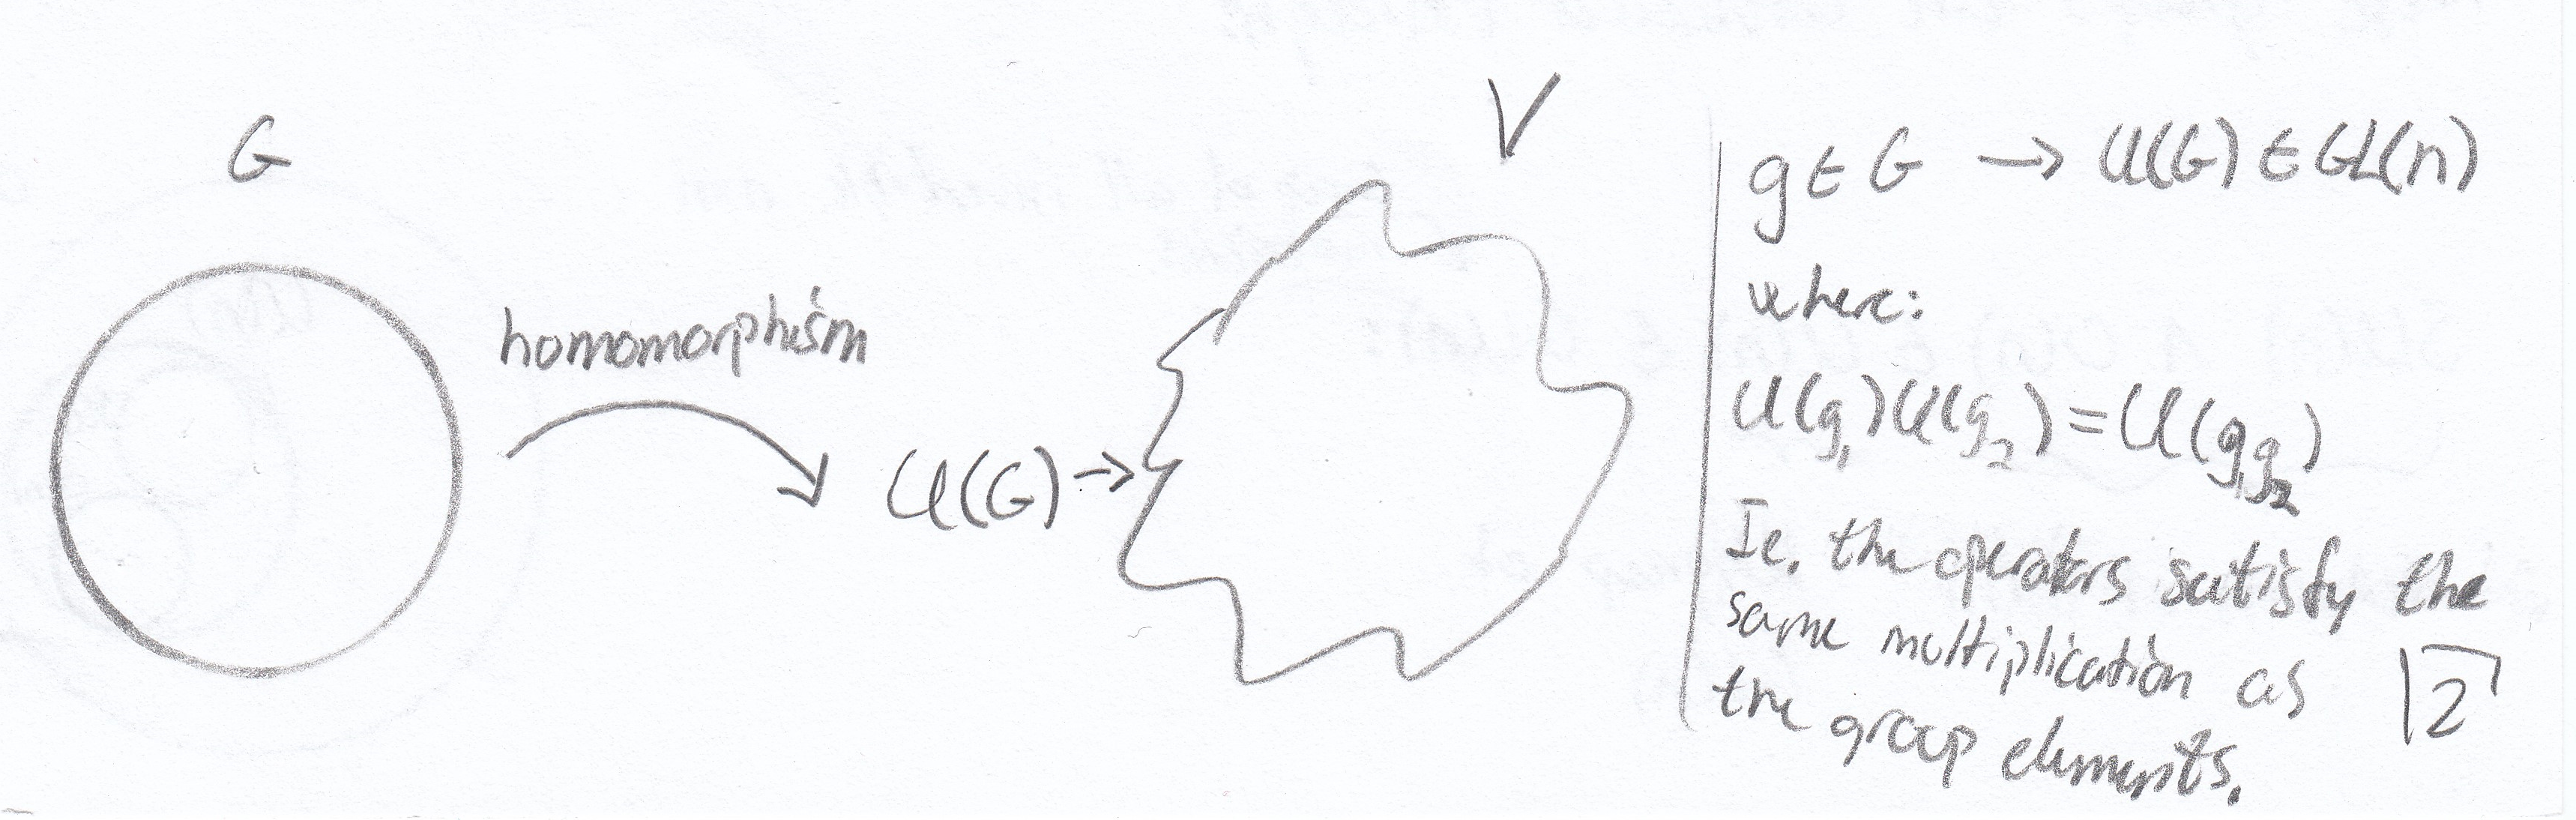
\includegraphics[width=0.6\textwidth]{figures//4}
	\caption{An illustration of a representation of a group.}
	\label{fig:4}
\end{figure} 
In terms of representations of Lie groups it is important to remember that a Lie group is defined in terms of the associated manifold. For this reason one can talk about different representations of groups made up by matrices\footnote{It is a confusing thought to think of representing matrices of a given dimension by other matrices with different dimensions. However, one should think of it like this; a given Lie group has an associated manifold. This manifold can have several representations. For example; $SU(2)$ is the group of $2\times 2$ unitary matrices with unit determinant. The manifold of this group is a circle. The manifold can be represented by either $2\times 2$ matrices or complex number (as is commonly done with the unit circle in complex space).} (eg. $SU(2)$). The representation of a Lie group is a representation of the associated manifold.

\paragraph{Invariant subspace:}\index{invariant subspace} Consider a representation, $U(g)$, of a group, $G$, defined on a linear vector space $V$. $V'\subseteq V$ is called an invariant subspace if for $v\in V'$; $U(g)v\in V'$, $\forall g\in G$. This means that if a vector in the invariant subspace $V'$ act on an arbitrary group element the transformed vector will always be again a part of the invariant subspace, $V'$. For an invariant subspace a representation $U'(g)$ of $G$ on $V'$, called a sub-representation of $U(g)$, can be defined viz
\begin{equation}
	U'(g)v=U(g)v,\quad \forall v\in V'.
\end{equation} 
This leads to the notion that the representation $U(g)$ is not a fundamental but instead composed of smaller building blocks. 

\paragraph{Irreducible representations:} An irreducible representation\index{Irreducible representation} is a representation of a group $G$ on a vector space $V$ that has no invariant subspaces besides $0$ and $V$ itself. Such representations can be thought of as truly fundamental since they are not made up of smaller representations. The irreducible representations of a group are the building blocks from which any other representation of the group can be built. A different approach to irreducible representations can be found by considering similarity transformations\index{Similarity transformation}. Given a matrix, $R$, and an invertible matrix, $S$, the similarity transformation is defined viz
\begin{equation}
	R\Rightarrow R'=S^{-1}RS.
\end{equation} 
If $R$ is a representation of the group $G$, then so is $R'$. An irreducible representation can be defined as a representation that cannot be transformed into block diagonal form via a similarity transformation.  

\paragraph{Generators of a discrete group: }
\index{Generators of a discrete group}
A collection, $c$, of elements of a discrete group, $G$, is said to be generators of the group if multiplication among the generators yield all elements of the group. 
\paragraph{Generators of a continuous group: }
\index{Generators of a continuous group}
In the case of a continuous group the generators are defined different, compared to the discrete group, since there are no single elements in a continuous group, but a continuum of elements. Consider a set of elements, $R$, that depends on some real, continuous parameters
\begin{equation}
	R=R(x,y,z,...).
\end{equation} 
These elements form a continuous group if $R$ fulfil the requirements for a group. If $R$ is differentiable, the group is a Lie group. Differentiability means that $R(dx)$ only differs infinitesimally from $R(0)=e$ by a term od order $dx$. Therefore $R(dx)$ can be parametrized as
\begin{equation}
	R(dx)=e-idxJ,
	\label{dj}
\end{equation} 
where $e$ is the identity element, the "$-i$" is included by convention (to make $J$ Hermitian) and $J$ is \emph{defined} as the generator of the group. By going from $dx\Rightarrow x$
\begin{equation}
	R(x)=\lim\limits_{N\Rightarrow \infty}\bigg(e-i\frac{dxJ}{N}\bigg)^N=e^{-ixJ}.
	\label{eq8}
\end{equation} 
In the considered case, used for illustrative purposes, there is only one parameter ($x$) and one corresponding generator ($J$). In general, a group can have several parameters ($\alpha_i$) and corresponding generators ($t_i$). The different generators make up a vector space. This vectors space is called a Lie algebra. 
\paragraph{Lie algebra:} A Lie algebra is a vector space, $\texttt{g}$, equipped with a binary operation (called the Lie bracket\footnote{The Lie bracket is often called the Lie algebra.}), $[,]: \texttt{g}\times \texttt{g}\Rightarrow \texttt{g}$. The binary operation satisfies the following axioms:
\begin{enumerate}
	\item Bilinearity:$[aX+bY,Z]=a[X,Z]+b[Y,Z]$ and $[Z,aX+bY]=a[Z,X]+b[Z,Y]$, for arbitrary numbers $a,b$ and $\forall X,Y,Z\in \texttt{g}$.
	
	\item Anticommutativity: $[X,Y]=-[Y,X]$ $\forall X,Y\in \texttt{g}$.
	
	\item The Jacobi identity: $[X,[Y,Z]]+[Z,[X,Y]]+[Y,[Z,X]]=0$ $\forall X,Y,Z \in \texttt{g}$. 
\end{enumerate}
The Lie algebra is therefore a vector space consisting of the generators of a Lie group. However, it is important to note that the definition of the Lie algebra makes no reference to any Lie group. Therefore the definition stands on its own and therefore one can talk about different Lie groups having the same Lie algebra. This leads to the definition of a distinguished Lie group.
\paragraph{Distinguished Lie group:} There is precisely one distinguished Lie group for each Lie algebra. The distinguished group has the property of being simply connected. This means that any closed curve on the manifold, corresponding to the Lie group, can be shrunk smoothly to a point. The simply connected group can be thought of as the "mother" of all those groups having the same Lie algebra, because there are maps to all other groups with the same Lie algebra from the simply connected group, but not vice versa. An intuitive name could be the "mother" group of a given Lie algebra. Formally the group is called the \emph{covering group}. All other groups with the same Lie algebra is said to be covered by the simply connected group.

\begin{example}
	Consider the group $SO(2)$. It is a one dimensional group describing rotations in $2$ dimensions. The group is one dimensional since only one continuous parameter, $\theta$, characterizes a rotation. The elements of the group can be represented by $2\times 2$ matrices which commute, and so the group is an abelian group. The group has one generator, $L$, which can be used to generate all elements of the group via
	\begin{equation}
		R(\theta)=e^{-i\theta L}.
	\end{equation} 
	Since the group is designated by $SO(2)$ each matrix is orthogonal an have unit determinant. 
\end{example}
\begin{example}
	This example will consider the isomorphism between $U(1)$ and $SO(2)$. As mentioned in example $4.2$ $SO(2)$ describes rotations in two dimensions and the group elements can be represented, in terms of the generator $L$, as
	\begin{equation}
		R(\theta)=e^{-i\theta L}.
	\end{equation} 
	$U(1)$ is the manifold of unitary $1\times 1$ matrices, i.e. unit complex numbers. The generator of the groups is the identity, $e$, and so the elements can be represented as
	\begin{equation}
		R(x)=e^{-ix}
	\end{equation} 
	There is an isomorphism between the two groups. This can be shown by considering
	\begin{equation}
		R(\theta_1)R(\theta_2)=e^{-i\theta_1 L}e^{-i\theta_2 L}=e^{-i(\theta_1+\theta_2) L}=R(\theta_1+\theta_2),
	\end{equation} 
	\begin{equation}
		f(x_1)f(x_2)=e^{-ix_1}e^{-ix_2}=e^{-i(x_1+x_2)}=f(x_1+x_2).
	\end{equation} 
	It is clear that there is a one-to-one correspondence between $x$ and $\theta$, and so $U(1)$ and $SO(2)$ are isomorphic to each other. The manifold associated with unit complex numbers is the unit circle in the complex plane. Since there is an isomorphism between $U(1)$ and $SO(2)$,the manifold of $SO(2)$ is likewise the unit circle in the complex plane. Hence, one can think of the Lie group as being the unit circle and the manifestation of the elements in complex numbers ($U(1)$) and matrices ($SU(2)$) as representations of the manifold. 
\end{example}


\section{$SO(3)$}
The group $SO(3)$ manifold corresponding to orthogonal $3\times 3$ matrices with unit determinant. The geometric shape of the manifold will be considered in the next section (on $SU(2)$). The reason for this is that $SU(2)$ is the simply connected group of the Lie algebra which it shares with $SO(3)$. Hence, the manifold of $SO(3)$ is a part of the manifold of $SU(2)$.\newline
The matrices describe rotations in $3d$ space. Formally; the $SO(3)$ group consists of all continuous, linear transformations in $3d$ Euclidean space which leave the length of coordinate vectors invariant. The elements of $SO(3)$ does not, in general, commute and so $SO(3)$ is, as opposed to eg. $U(1)$ or $SO(2)$, a non-abelian Lie group.\newline
A generic rotation in $3d$ is parametrized by $3$ rotations, by $3$ continuous angles, around the three coordinate axis. Corresponding to each continuous parameter is a generator, and so $SO(3)$ has $3$ basis generators. The rotations around a given axis form a subgroup of $SO(3)$ that is isomorphic to $SO(2)$. Since there are $3$ coordinate axis' there are $3$ basis generators, denoted by $J_i$. the Lie bracket of the generators is given by
\begin{equation}
	[J^i,J^j]=i\epsilon^{ijk}J^k.
\end{equation} 
From the basis generators a generic element of $SO(3)$ can be described as
\begin{equation}
	R(\alpha,\beta,\gamma)=R_3(\gamma)R_2(\beta)R_1(\alpha)=e^{-iJ_3\gamma}e^{-iJ_2\beta}e^{-iJ_1\alpha},
\end{equation} 
where $\alpha,\beta,\gamma$ are \emph{Euler angles} and the basis matrices $R_i$ are given by
\begin{equation}
	\begin{split}
		&R_1(\alpha)=\begin{bmatrix}
			1 & 0 & 0 \\
			0 & cos(\alpha) & sin(\alpha)\\
			0 & -sin(\alpha) & cos(\alpha)\\
		\end{bmatrix},\\
		& 
		R_2(\beta)=\begin{bmatrix}
			cos(\beta) & 0 & -sin(\beta) \\
			0 & 1 & 0\\
			sin(\beta) & 0 & cos(\beta)\\
		\end{bmatrix},\\
		& 
		R_3(\gamma)=\begin{bmatrix}
			cos(\gamma) & sin(\gamma) & 0 \\
			-sin(\gamma) & cos(\gamma) & 0\\
			0 & 0 & 1\\
		\end{bmatrix},
	\end{split}
	\label{rot}
\end{equation} 
where $R_i$ rotate the coordinate system, not the vector. It is a choice of convention. Rotating the vector is called an active transformation whereas rotating the coordinate system is called a passive transformation. Since the placement of a coordinate system is entirely up to the physicist, i.e. the coordinate system is not a physical thing, it makes more intuitive sense to alternate your definition than actually going in and rotating the physical vector. Hence, here the approach of passive transformations is used.

\section{$SU(2)$}
The group $SU(2)$ is manifold corresponding to unitary $2\times 2$ matrices with unit determinant. The manifold of $SU(2)$ is found by extending the method used to discover the manifold of $SO(2)$. In discovering the manifold of $SO(2)$ it was used that $SO(2)$ is isomorphic to $U(1)$, i.e. sharing manifold, and that $U(1)$ consists of two dimensional complex, unitary numbers which are defined on the unit circle in the complex plane. Extending this analogy the manifold of $SU(2)$ can be found as the manifold of 4 dimensional complex, unitary numbers; quaternions. To describe 4 dimensional complex numbers three imaginary units are needed - As opposed to one imaginary unit for two dimensional complex numbers ($i$). The three imaginary units are defined viz
\begin{equation}
	i^2=j^2=k^2=ijk=-1.
\end{equation} 
Then a 4 dimensional complex number, a quaternion, can be parametrized viz
\begin{equation}
	q=a+bi+cj+dk.
\end{equation} 
The set of unit quaternions are those that satisfy
\begin{equation}
	qq^\dagger=a^2+b^2+c^2+d^2=1.
\end{equation} 
Just as complex numbers can be represented as matrices by mapping the complex unit ($i$) to a matrix, so can quaternions. Specifically~\citep{Schwichtenberg2015}
\begin{equation}
	I=\begin{bmatrix}
		1 & 0\\
		0 & 1\\
	\end{bmatrix}, \quad \hat{i}=\begin{bmatrix}
		i & 0 \\
		0 & -i \\
	\end{bmatrix}, \quad \hat{j}=\begin{bmatrix}
		0 & 1\\
		-1 & 0 \\
	\end{bmatrix}, \quad \hat{k}=\begin{bmatrix}
		0 & i \\
		i & 0 \\
	\end{bmatrix}.
\end{equation} 
This means the generic quaternion can be parametrized viz
\begin{equation}
	q=aI+b\hat{i}+c\hat{j}+d\hat{k}=\begin{bmatrix}
		a+ib & c+id\\
		-c+id & a-ib\\
	\end{bmatrix}\Rightarrow det(q)=a^2+b^2+c^2+d^2.
	\label{as}
\end{equation} 
Comparing equation \eqref{as} to the definition of unit quaternions ($qq^\dagger=1$), it is clear that the matrices must be unitary and have unit determinant. That is the matrices make up the group $SU(2)$. Hence, unit quaternions are isomorphic to $SU(2)$ just like $U(1)$ is isomorphic to $SO(2)$. Hence, the manifold of $SU(2)$ can be described by the unit quaternions. The unit quaternions are characterized by $a^2+b^2+c^2+d^2=1$, analogous to how 2 dimensional unit complex numbers are characterized by $z=a+ib\Rightarrow a^2+b^2=1$. $a^2+b^2=1$ describes the unit circle, $S^1$. Hence, the manifold of two dimensional unit complex numbers is the unit circle in the complex plane. Likewise $a^2+b^2+c^2+d^2=1$ describes the unit three sphere, $S^3$. Hence, the manifold of four dimensional unit complex numbers is the unit three sphere. The unit three sphere is a simply connected manifold. Hence, $SU(2)$ is simply connected.

\subsection{Relationship between $SO(3)$ and $SU(2)$}
To relate the two groups it will be investigated how quaternions can be used to rotate a vector. Parametrizing a vector viz
\begin{equation}
	v=v_x\hat{i}+v_y\hat{j}+v_z\hat{k}=\begin{bmatrix}
		iv_x & v_y+iv_z\\
		-v_y+iv_z & -iv_x\\
	\end{bmatrix}\Rightarrow det(v)=x^2+y^2+z^2.
	\label{as4}
\end{equation} 
The determinant of $v$ is the length of the vector. Since the length of a vector is conserved during a rotation, the transformation must preserve determinants. This means restricting ourselves to unit quaternions as a means to transform the vector
\begin{equation}
	v\Rightarrow v'=q^{-1}vq,
	\label{as1}
\end{equation} 
where once again the approach of passive transformations has been applied. The inverse transformation, $qvq^{-1}$, is the corresponding active rotation\footnote{$qvq^{-1}$ is just a the inverse transformation of $q^{-1}vq$. This makes intuitively sense since rotating a vector in one direction is equivalent to rotating the coordinate system in the opposite direction. Hence, the definition of active and passive rotations is related to the definition of positive and negative angles also.}. In order to relate the transformation of equation \eqref{as1} to rotations the rotation angles must be introduced. In this regard it is convenient to parametrize the unit quaternion viz
\begin{equation}
	q=cos(\theta)+sin(\theta)||\vec{e}||,
\end{equation} 
where $||\vec{e}||$ is the normalized rotation axis. For transparency consider a rotation of $\frac{\vec{x}}{|\vec{x}|}\equiv \hat{x}$ around the $z$-axis. In this case
\begin{equation}
	q=cos(\theta)I+sin(\theta)k=\begin{bmatrix}
		cos(\theta) & isin(\theta)\\
		isin(\theta) & cos(\theta)\\
	\end{bmatrix}.
	\label{as2}
\end{equation} 
Using equation \eqref{as2}
\begin{equation}
	q^{-1}\hat{i}q=\begin{bmatrix}
		cos(\theta) & -isin(\theta)\\
		-isin(\theta) & cos(\theta)\\
	\end{bmatrix}\begin{bmatrix}
		i & 0\\
		0& -i\\
	\end{bmatrix}\begin{bmatrix}
		cos(\theta) & isin(\theta)\\
		isin(\theta) & cos(\theta)\\
	\end{bmatrix}=\begin{bmatrix}
		icos(2\gamma) & -sin(2\theta)\\
		sin(2\theta) & -icos(2\theta)\\
	\end{bmatrix}.
	\label{as3}
\end{equation} 
Comparing equation \eqref{as3} to equation \eqref{as4}
\begin{equation}
	\begin{split}
		&v_x\Rightarrow v'_x=cos(2\theta),\\
		&v_y\Rightarrow v'_y=-sin(2\theta),\\
		&v_z\Rightarrow v'_z=0.\\
	\end{split}
	\label{as5}
\end{equation} 
Rotating a vector in 3-space reveals, cf. equation \eqref{rot}
\begin{equation}
	R_3(\gamma)\hat{x}
	\begin{bmatrix}
		cos(\gamma) & sin(\gamma) & 0 \\
		-sin(\gamma) & cos(\gamma) & 0\\
		0 & 0 & 1\\
	\end{bmatrix}\begin{bmatrix}
		1\\0 \\0\\
	\end{bmatrix}=\begin{bmatrix}
		cos(\gamma)\\
		-sin(\gamma)\\
		0\\
	\end{bmatrix}.
	\label{as6}
\end{equation} 
By comparing equation \eqref{as5} and \eqref{as6} it is clear that $\gamma=2\theta$. That is, in rotating $\hat{x}$ by $\theta$ the vector is rotated by $2\gamma$ in 3-space. This means that there is a two-to-one map from the manifold of $SU(2)$ to the manifold of $SO(3)$, i.e. there are two elements in the manifold of $SU(2)$ that corresponds to the same element in the manifold of $SO(3)$. Hence given one element of the manifold of $SU(2)$ one can find the corresponding element in the manifold of $SO(3)$ but not vice versa. this confirms that the manifold of $SU(2)$ is indeed simply connected. Since there is a two-to-one correspondence between the manifolds of $SU(2)$ and $SO(3)$, and the manifold of $SU(2)$ is the unit three sphere, the manifold of $SO(3)$ must be half a unit three sphere. Since the manifold of $SU(2)$ covers the manifold of $SO(3)$ twice it is called the double cover of the manifold of $SO(3)$.

\section{The Lorentz group}
\label{sec:lor}
The Lorentz group\index{The Lorentz group}, denoted by\footnote{Three space-like dimensions and one time-like dimension.} $O(3,1)$, is the group representing the coordinate transformations of $SR$; boosts and rotations that is. Because the Lorentz group describes the transformations of SR, which are transformations of four vectors, the Lorentz groups is often analysed in a certain representation; the vector representation. In the vector representation an event in SR is described by a four vector on the form
\begin{equation}
	x^\mu\equiv \begin{bmatrix}
		t \\
		\vec{x}\\
	\end{bmatrix}.
\end{equation} 
This vector is called contravariant (index up) and it is defined by its transformation properties
\begin{equation}
	dx^\mu\Rightarrow d{x'}^\mu=\underbrace{\frac{\partial {x'}^\mu}{\partial x^\nu}}_{\Lambda^\mu_{\,\,\,\nu}}dx^\nu.
	\label{contra}
\end{equation} 
Any vector that transforms in this way is called a contravariant vector. Likewise, a covariant vector is defined by
\begin{equation}
	dx_\mu\Rightarrow d{x'}_\mu=\underbrace{\frac{\partial {x'}_\mu}{\partial x_\nu}}_{(\Lambda^{-1})^\nu_{\,\,\,\mu}=\Lambda_\mu^{\,\,\,\nu}}dx_\nu.
\end{equation} 
The contra-variant and covariant vectors are related by the metric via
\begin{equation}
	x^\mu=g^{\mu\nu}x_\nu.
\end{equation} 
During the coordinate transformations, the length of the vectors, $x^\mu x_\mu\equiv x\cdot x=x^2$, is invariant. The length of a vector can be expressed via the metric
\begin{equation}
	x^\mu x_\mu=g_{\mu\nu}x^\mu x^\nu=g_{\mu\nu}x'^\mu x'^\nu=g_{\mu\nu}\Lambda^\nu_{\,\,\,\,\alpha}\Lambda^\mu_{\,\,\,\,\beta}x^\alpha x^\beta.
\end{equation} 
Rearranging the dummy indices
\begin{equation}
	g_{\mu\nu}x^\mu x^\nu=g_{\alpha\beta}\Lambda^\alpha_{\,\,\,\nu}\Lambda^\beta_{\,\,\,\mu}x^\nu x^\mu\Rightarrow g_{\mu\nu}=g_{\alpha\beta}\Lambda^\alpha_{\,\,\,\nu}\Lambda^\beta_{\,\,\,\mu},
\end{equation} 
which can be written $g=\Lambda^Tg\Lambda$ in matrix notation. Taking the determinant, and using that $g_{\mu\nu}=\eta_{\mu\nu}=diag(1,-1,-1,-1)$ for Minkowski space
\begin{equation}
	det(\eta)=det(\Lambda^T)det(\eta)det(\Lambda)\Rightarrow det(\Lambda^T)det(\Lambda)=1.
\end{equation} 
Use now that $det(\Lambda^T)=det(\Lambda)$ to find $det(\Lambda)^2=1\Rightarrow det(\Lambda)=\pm 1$. Transformations for which $det(\Lambda)= 1$ are called proper. Transformations for which $det(\Lambda)= -1$ are called improper. Another classification comes from
\begin{equation}
	g_{00}=1=\Lambda^\alpha_{\,\,\,0}\Lambda^\beta_{\,\,\,0}g_{\alpha\beta}=(\Lambda^0_{\,\,\,0})^2-\sum_{i=1}^{3}(\Lambda^i_{\,\,\,0})^2\Rightarrow |\Lambda^0_{\,\,\,0}|>1.
\end{equation} 
This allows $\Lambda^0_{\,\,\,0}>1$ or $\Lambda^0_{\,\,\,0}<-1$. The transformations characterized by $\Lambda^0_{\,\,\,0}>1$ are called orthochronous whereas transformations characterized by $\Lambda^0_{\,\,\,0}<-1$ are called non-orthochronous. Hence, the Lorentz transformations can be grouped into $4$ categories\footnote{That this is correct can be seen by considering the $TP\Lambda^{po}$-term; the determinant must be positive since it is proper. The determinant of $\Lambda^{po}$ is defined as positive and since the determinant is distributive and negative for both $T,P$, the table must be as shown. The table is confirmed by \citet{Srednicki2027}.} shown in figure \ref{fig:5}.
\begin{figure}[H]
	\captionsetup{width=1\textwidth}
	\centering
	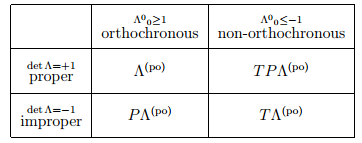
\includegraphics[width=0.4\textwidth]{figures//5}
	\caption{The different categories of Lorentz transformations.}
	\label{fig:5}
\end{figure} 
As shown in figure \ref{fig:5} the different elements of the categories can all be expressed in terms of proper, orthochronous transformations followed by a time-inversion and/or parity operation. Parity is called the "mirror-transformation". Until 1956 physicists believed all physical systems should be invariant under parity. However, in 1956 it was found that the weak interaction violates parity. Mathematically, parity is expressed viz
\begin{equation}
	\Lambda_P x=\begin{bmatrix}
		t\\
		-\vec{x}\\
	\end{bmatrix}, \quad \text{and} \quad  \Lambda_Pp=\begin{bmatrix}
		p^0\\
		-\vec{p}\\
	\end{bmatrix},
\end{equation} 
where $\Lambda_P=diag(1,-1,-1,-1)$ in the vector representation\footnote{Not in general, only in the vector representation.}. Similarly, time-inversion is given by
\begin{equation}
	\Lambda_T x=\begin{bmatrix}
		-t\\
		\vec{x}\\
	\end{bmatrix}, \quad \text{and} \quad  \Lambda_Tp=\begin{bmatrix}
		-p^0\\
		\vec{p}\\
	\end{bmatrix},
\end{equation} 
where $\Lambda_T=diag(-1,1,1,1)$ in the vector representation\footnote{Not in general, only in the vector representation.}. Since the subsets that are not elements of the proper orthochronous subgroup can be determined via applying parity and/or time-inversion, the elements of the proper, orthochronous subgroup is of special interest. Since all elements of the Lorentz group is enclosed in $O(3,1)$, and proper means $det(\Lambda)=1$, the proper, orthochronous transformations (indeed all proper transformations) are members of $SO(3,1)$- in this case a subgroup of $O(3,1)$. $SO(3,1)$ is also called the proper Lorentz group, but most often it is just referred to as the Lorentz group. $SO(3)$ consists of all boost, rotations and combinations of the two. A generic element of the proper, orthochronous subgroup of the Lorentz group can therefore be expressed as
\begin{equation}
	\Lambda^\mu_{\,\,\,\nu}=\Lambda(R')^\mu_{\,\,\,\alpha}\Lambda(\gamma)^\alpha_{\,\,\,\beta}\Lambda(R)^\beta_{\,\,\,\nu}.
\end{equation} 
The $\Lambda$-matrices form a representation of the Lorentz group.

\begin{example}
	\index{4-vector}
	\index{Current density}
	\index{Four current}	
	\emph{Prove that $J^\mu$ is a $4$-vector, where}\newline
	\begin{equation}
		J^\mu=\begin{bmatrix}
			\rho\\
			J_x\\
			J_y\\
			J_z\\
		\end{bmatrix}=\begin{bmatrix}
			\rho\\
			\rho v_x\\
			\rho v_y\\
			\rho v_z\\
		\end{bmatrix}=\begin{bmatrix}
			\rho\\
			\vec{J}\\
		\end{bmatrix}.
	\end{equation} 
	An $n$-dimensional vector is a physical object that can be represented as a $n\times1$ matrix. Because a vector can be represented as a matrix, it must obey the rules of linear algebra, including scalar multiplication, vector addition, dot product, scalar and vector projections. Further more a vector is a rank 1 tensor, which means that it must transform in a well defined way during a coordinate transformation; it must conserve its length during a coordinate transformation. This last definition will be used to verify that $J^\mu$ is in fact a 4-vector. For a $4$-vector the length is called the spacetime interval ($ds^2$). Consider a volume ($V_1$) of charge moving with a uniform velocity ($v_{1x}$) as observed from the reference frame $S_1$\footnote{I only consider movement along the $x$-axis to illustrate the principle. A general treatment is rather cumbersome.}. In this frame the spacetime interval will be given by
	\begin{equation}
		ds_1^2=\rho_1^2(v_{1x}^2-1),
	\end{equation} 
	where the $y$ and $z$ components of the velocity is zero and the subscript on $ds_1$ is introduced because current density has not been proven a $4$-vector yet (and therefore that $ds$ for different reference frames is the same). From $S_1$ the volume containing the charge is contracted via.
	\begin{equation}
		V_1=\gamma^{-1}(v_{1x})V_0,
	\end{equation} 
	where $\gamma=\gamma(v)=(1-v^2)^{-\frac{1}{2}}$. The volume is contracted in the direction parallel to the direction of motion, and hence the volume is diminished as seen from $S_1$. Considering the scenario from the reference frame of $S_2$, which moves with a uniform velocity $v$ with respect to $S_1$ and parallel to the $x$-axis of $S_1$, the volume is seen to be moving with $v_{2x}$. Here the volume is observed to be
	\begin{equation}
		V_2=\gamma^{-1}(v_{2x})V_0.
	\end{equation} 
	Using that
	\begin{equation}
		v_{2x}=\frac{v_{1x}-v}{1-vv_{1x}}.
	\end{equation} 
	The volumes in the two reference frames can be related in terms of the velocity in one reference frame. For example
	\begin{equation}
		\frac{V_1}{V_2}=\gamma(v)(1-vv_{1x}).
	\end{equation} 
	This relation can be used to determine how the charge density transforms. There must be conservation of charge ($Q=\rho_iV_i$) between reference frames. Therefore
	\begin{equation}
		V_1\rho_1=V_2\rho_2\Rightarrow \rho_2=\rho_1\frac{V_1}{V_2}=\rho_1\gamma(v)(1-vv_{1x}).
	\end{equation} 
	Using this to express $ds_2^2$
	\begin{equation}
		ds_2^2=\rho_2^2(v_{2x}^2-1)=\bigg(\rho_1\gamma(v)(1-vv_{1x})\bigg)^2\bigg(\bigg(\frac{v_{1x}-v}{1-vv_{1x}}\bigg)^2-1\bigg)=\rho_1^2(v_{1x}^2-1)=ds_1^2.
	\end{equation} 
	The space time interval is conserved ($ds_1=ds_2$), and $J^\mu$ is therefore a $4$-vector. One can also say that $\rho$, as has been shown for the $x$-component, transforms via the Lorentz-transformation and therefore the length of the $4$-vector transforms from reference frame to reference frame via
	\begin{equation}
		J'^\mu J_\mu'={\Lambda_x}(v)^\mu_\nu {\Lambda^{-1}_x}(v)^\nu_\mu J^\nu J_\nu=J^\nu J_\nu,
	\end{equation} 
	where $L$ is the Lorentz matrix
	\begin{equation}
		\Lambda_x(v)=\begin{bmatrix}
			\gamma & -v\gamma & 0 & 0\\
			-v \gamma & \gamma & 0 & 0\\
			0 & 0 & 1 & 0\\
			0 & 0 & 0 & 1
		\end{bmatrix}.
	\end{equation} 
	As is apparent the length of the vector is conserved as it should be in order for $J^{\mu}$ to be a vector.
\end{example}


\begin{example}
	\emph{A spaceship travels with a velocity, $\vec{v}^T=\frac{1}{2}\begin{bmatrix}
			1 & 1 & 1\\
		\end{bmatrix}$, when it is hit by a cosmic ray carrying a four momentum, $p^T=\begin{bmatrix}
			300 & 299 & 0& 0\\
		\end{bmatrix}\cdot10^{-27}kg$.}
	\begin{figure}[H]
		\captionsetup{width=1\textwidth}
		\centering
		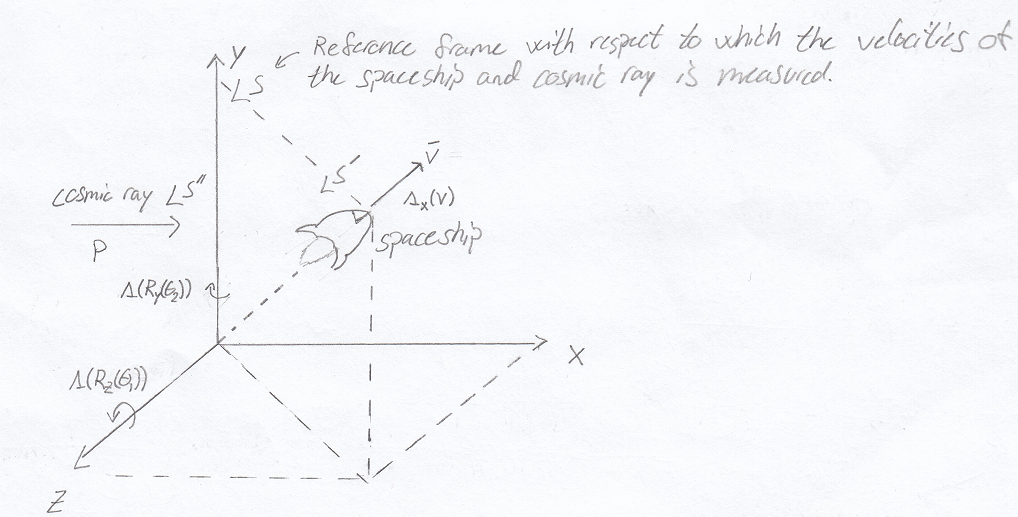
\includegraphics[width=0.6\textwidth]{figures//ss}
		\caption{The scenario with the three reference frames involved.}
		\label{fig:ss}
	\end{figure} 
	\begin{enumerate}
		\item \emph{Find the four velocity, $u$, of the spaceship.}
		
		From $S$
		\begin{equation}
			u=\gamma(v)\begin{bmatrix}
				1 \\
				\vec{v}\\
			\end{bmatrix}=\begin{bmatrix}
				2 \\
				2\vec{v}\\
			\end{bmatrix},
		\end{equation} 
		where $v=|\vec{v}|$.
		
		\item \emph{Find the energy of the cosmic ray in $S'$.}
		
		I know the energy in $S$ from $p$, so I will create a Lorentz transformation to transform $p$ from $S$ to $S'$. To this end I will use a general Lorentz transformation which will consist of two rotations, one boost and the inverse rotations. The idea is to rotate the coordinate-system so it aligns with the velocity of the space-ship, boost so the coordinate system, in rotated form, moved with the spaceships, and lastly rotate the coordinate system back. The result will be a boost of $S$ such that is follows the spaceship, i.e. $S\Rightarrow S'$. First, I will rotate (counter clockwise, i.e. positive angle) around the $z$-axis such that the $\vec{v}$lies in the $zx$ plane. Hereafter I will rotate (clockwise, i.e. negative angle) around the (new, since I have rotated around the $z$-axis) $y$-axis such that the $x$-axis is aligned with $\vec{v}$. Hereafter I will boost along the $x$-axis and rotate back. The Lorentz transformation
		\begin{equation}
			\Lambda_{tot}=\big(\Lambda(R_y(\theta_2))\Lambda(R_z(\theta_1))\big)^{-1}\Lambda_x(\gamma(v))\Lambda(R_y(\theta_2))\Lambda(R_z(\theta_1),
		\end{equation} 
		where
		\begin{equation}
			\Lambda(R_i(\theta_j))=\begin{bmatrix}
				1 & 0 & 0 & 0\\
				0 &   &   &   \\
				0 &   & R_i(\theta_j) & \\
				0 &   &   & \\
			\end{bmatrix}, \quad \Lambda_x(\gamma(v))=\begin{bmatrix}
				\gamma(v)&-v\gamma(v)&0&0\\
				-v\gamma(v)&\gamma(v)&0&0\\
				0&0&1&0\\
				0&0&0&1\\
			\end{bmatrix}.
		\end{equation} 
		Since I know $v$, all I need is the two rotation angles. I find these by considering the criterion for each rotation. After the first rotation the velocity should be in the $zx$-plane, and therefore the transformed velocity should have no $y$-component. Hence, I can find the first rotation angle from
		\begin{equation}
			\begin{split}
				R_z(\theta_1)\vec{v}&\propto\begin{bmatrix}
					cos(\theta_1) & sin(\theta_1) & 0 \\
					-sin(\theta_1) & cos(\theta) & 0 \\
					0 & 0 & 1 \\
				\end{bmatrix}\begin{bmatrix}
					1\\
					1\\
					1\\
				\end{bmatrix}\\
				&=\begin{bmatrix}
					cos(\theta_1)+sin(\theta_1)\\
					sin(\theta_1)-cos(\theta_1)\\
					1\\
				\end{bmatrix}\\
				&= \begin{bmatrix}
					\dots\\
					0\\
					1\\
				\end{bmatrix}.\\
			\end{split}
		\end{equation} 
		In order for the second component of the transformed velocity to vanish $sin(\theta_1)=cos(\theta_1)\Rightarrow \theta_1=\frac{\pi}{4}$. From the second rotation the $x$-axis is to align with $\vec{v}$, so the third component of the transformed velocity is to vanish. Hence, I can find the second rotation angle from
		\begin{equation}
			\begin{split}
				R_y(\theta_2)R_z(\theta_1)\vec{v}&\propto
				\begin{bmatrix}
					cos(\theta_2) & 0 & -sin(\theta_2) \\
					0 & 1 & 0 \\
					sin(\theta_2) & 0 & cos(\theta_2) \\
				\end{bmatrix}\begin{bmatrix}
					\sqrt{2}\\
					0\\
					1\\
				\end{bmatrix}\\
				&=\begin{bmatrix}
					\sqrt{2}cos(\theta_2)-sin(\theta_2)\\
					0\\
					cos(\theta_2)+\sqrt{2}sin(\theta_2)\\
				\end{bmatrix}\\
				&=\begin{bmatrix}
					|\vec{v}|\\
					0\\
					0\\
				\end{bmatrix}.\\
			\end{split}
		\end{equation} 
		In order for the third component of the transformed velocity to vanish; $cos(\theta_2)+\sqrt{2}sin(\theta_2)=0\Rightarrow \theta_2=-35.264 deg$. By using the two rotation angles I can now transform $p$ and find it in $S'$
		\begin{equation}
			p'=\Lambda_{tot}p=\begin{bmatrix}
				301 \\
				296/3\\
				-601/3\\
				-601/3\\
			\end{bmatrix}\cdot 10^{-27}kg.
		\end{equation} 
		Hence, the energy (now in SI units) as seen from $S'$ is $301\cdot 10^{-27}kg\cdot c^2\simeq 2.7\cdot 10^{-8}J$.
		
		\item \emph{Calculate the energy in $S'$ from $-g_{\mu\nu}u^\mu p^\nu$. Why does this work?}
		
		I can also calculate the energy from $-g_{\mu\nu}u^\mu p^\nu$. $-g_{\mu\nu}u^\mu p^\nu$ has all indices contracted and so is a Lorentz scalar. In the rest frame of the spaceship $u^T=\begin{bmatrix}
			1 \\\vec{0}\\
		\end{bmatrix}$ and so it works to pick out the zeroth component of the momentum vector; the energy. So, the quantity is the energy in $S'$ and it is invariant between reference frame. Hence, I can calculate it in $S$ and thereby obtain the energy in $S'$. I find
		\begin{equation}
			\begin{split}
				-g_{\mu\nu}u^\mu p^\nu&=u^0p^0-u^1p^1-u^2p^2-u^3p^3\\
				&=(2\cdot 300-299)\cdot 10^{-27}kg\cdot c^2\\
				&=301\cdot 10^{-27}kg\cdot c^2.
			\end{split}
		\end{equation} 
	\end{enumerate}
\end{example}

\section{The Poincare' group}
The Poincare' group, $ISO(1,3)$, is the group of Lorentz transformations and translations. The Poincare' group encompasses the transformations the physical theories, in the absence of general relativistic effects, should obey, i.e. the physical theory should be invariant under translation, rotation and boosts - Physical theories should be invariant under Poincare' transformations. A generic Poincare' transformation is on the form
\begin{equation}
	x^\mu\Rightarrow {x'}^\mu=\Lambda^{\mu}_{\,\,\, \nu}x^\nu+a^{\mu}.
\end{equation}  
where $a^\mu$ is a constant four vector. From which it is clear that the Poincare' group contains Lorentz transformations and translations. The generators of the Poincare' group are the generators of the Lorentz group, $J_i,K_i$ and the generator of translation in flat space-time (Minkowski space); $p^\mu$. In terms of the generators, the algebra reads
\begin{equation}
	\begin{split}
		&[J_i,J_j]=i\epsilon_{ijk}J_k, \quad [J_i,K_j]=i \epsilon_{ijk}K_k, \quad [K_i,K_j]=-i\epsilon_{ijk}J_k,\\
		&[J_i,p_j]=i\epsilon_{ijk}p_k,\quad [j_i,p_0]=0,\quad [k_i,p_j]=i\delta_{ij}p_0,\quad [k_i,p_0]=-ip_i.
	\end{split}
\end{equation} 


\chapter{Classical field theory}
Field theory is one of the cornerstones of classical physics. The most notable examples of classical fields are the force fields that one encounters in the description of gravitational and electromagnetic phenomena. These fields are caused by the presence of masses and electric charges, respectively. In this chapter I present a framework for classical field theory, which is known as the Lagrangian formulation, alongside a vital theorem relating mathematical symmetries of the Lagrangian to conserved quantities; Noethers theorem.

\section{The Lagrangian formulation of classical field theory}
The framework of classical field theory is the generalization of Lagrangian mechanics to fields. The formulation of Lagrangian mechanics made for classical mechanics was for a finite number of degrees of freedom - fields incorporate an infinite number of degrees of freedom and as such the Lagrangian formalism must be generalized to encompass this scenario. In order to do so the classical Lagrangian is expressed, not as a function of dynamical variables that are functions of time (i.e. $q_i(t)$), but as a function of functions (fields) of space-time\footnote{A function of a function is a functional. Hence, in generalizing the Lagrangian formalism from classical mechanics to classical field theory the Lagrangian goes from being a function to being a functional.}. For a local field theory, a generic Lagrangian ($L$) can be written in terms of the Lagrangian density ($\mathcal{L}$) which is a function of the generic fields ($\phi_a(x)$) and their derivatives ($\partial_\mu\phi_a(x)$),  i.e.
\begin{equation}
	L[\phi_a(x),t]=\int d^3x\mathcal{L}(\phi_a(x),\partial_\mu\phi_a(x)).
\end{equation} 
The Lagrangian density is related to the Hamiltonian density cf.
\begin{equation}
	\mathcal{H}=\sum_a\Pi_a\partial_0\phi_a-\mathcal{L},
	\label{h1}
\end{equation} 
which is in complete analogy with the definition of the Hamiltonian in classical mechanics (see equation \eqref{ham}). In both classical and quantum field theory the theories are formulated in terms of a Lagrangian density because the Lagrangian density is manifestly Lorentz invariant. In general the physical laws are required to be covariant under Poincare' transformations (translations, rotations and boosts). Poincare' covariance is a statement of the familiar principle from classical mechanics; physics should be the same in inertial reference frames. The fields in the action are inherently independent of translations\footnote{The action is invariant under a constant coordinate transformation since this can be absorbed by the integration measure. Take $S=\int d^4x\mathcal{L}(\phi(x),\dots)\Rightarrow S'=\int d^4x\mathcal{L}(\phi(x+a),\dots)=\int d^4y\mathcal{L}(\phi(y),\dots)=S$, where $y=x+a$. Hence, the action is inherently invariant under coordinate translations.}. Hence, the action is only "forced" to be covariant under Lorentz transformations. Since the action is a Lorentz scalar, the Lagrangian density is also the be Lorentz invariant. 

\paragraph{Lorentz covariance:} \emph{A quantity is called Lorentz covariant if the form of the equation does not change under a Lorentz  transformation\index{Lorentz covariance}. An object is Lorentz covariant if it transforms under an irreducible representation of the Lie algebra of the proper, orthochronous Lorentz group.} 

\paragraph{Lorentz invariance:} \emph{A term is Lorentz invariant if it does not change during a proper, orthochronous Lorentz transformation. An object that does not change under proper, orthochronous Lorentz transformations is called a Lorentz scalar.}\newline

To recap; Lorentz covariance is directly derived from the principle that physics should be the same in inertial reference frames. Enforcing Lorentz covariance means that the fields in the Lagrangian density should transform under irreducible representations of the Lie algebra of the proper, orthochronous Lorentz group. In the next section the representations will be derived. Subsequently these representations can be arranged such that the resulting objects are invariant under parity - Which must physical systems are observed to be\footnote{Specifically the spinors are not invariant under parity. Hence, they are arranged in the Dirac spinor which is.}! 

\section{Irreducible (finite) representations of the Lorentz group}
Here the irreducible representations of the Lie algebra of the proper, orthochronous Lorentz group (or equivalently; the irreducible representations of the covering group of the proper, orthochronous Lorentz group) will be determined. The proper, orthochronous Lorentz group is not a simply connected group and as such there is not a one-to-one correspondence between the irreducible representations of the Lie algebra and the the representations of the proper, orthochronous Lorentz group. Instead, there is a one-to-one correspondence between the irreducible representations of the Lie algebra and the covering group of the proper, orthochronous Lorentz group. Hence, when one talks about the irreducible (finite\footnote{"Finite" is used because there is also an infinite dimensional representation of the cover of the proper, orthochronous Lorentz group. These are the matrices responsible for Lorentz transforming $x$. When a field is transformed the field itself is transformed via a finite dimensional representation of the cover of the proper, orthochronous Lorentz group whereas the argument of the field is transformed via the infinite dimensional representation of the cover of the proper, orthochronous Lorentz group. However, how to transform the position four vector in special relativity has already been covered and as such the infinite dimensional representation will not be considered here.}) representations of the Lorentz group, one really talks about the irreducible representations of the covering group (double cover) of the proper, orthochronous Lorentz group. Recall that a covering group is a group which manifold is simply connected. For this reason, groups which have identical Lie algebra must have a manifold that is contained inside the manifold of the covering group. An example is $SU(2)$ and $SO(3)$ (the two groups have the same Lie algebra); the manifold of $SU(2)$ is the unit three sphere whereas the manifold of $SO(3)$ is half the unit three sphere. Since the unit three sphere is simply connected, $SU(2)$ is the simply connected group of this Lie algebra and the manifolds of groups having identical Lie algebra is contained/covered by the manifold of $SU(2)$. The covering group of the proper, orthochronous Lorentz group is $SL(2,\mathbb{C})$; the group of non-degenerate complex matrices with unit determinant. Hence the irreducible representations obtained from the Lie algebra of the proper, orthochronous Lorentz group are the irreducible representations\footnote{Only some of the irreducible representations of the Lie algebra of the proper, orthochronous Lorentz group will be irreducible representations of the proper orthochronous Lorentz group (eg. the spinor representations are not irreducible representations of the proper, orthochronous Lorentz group).} of $SL(2,\mathbb{C})$, and it is these representations that the objects in the Lagrangian density is required to transform under in order to be Lorentz covariant.\newline

To determine the irreducible representations of the covering group of the proper, orthochronous Lorentz group I will begin by considering a field (not necessarily hermitian) that carries a generic Lorentz index, $\phi_a(x)$. Under a Lorentz transformation on the form $x^\mu\Rightarrow {x'}^\mu=\Lambda^\mu_{\,\,\, \nu}x^\nu$ the generic field transforms viz
\begin{equation}
	\phi_a(x^\mu)\Rightarrow \phi'_a({x'}^\mu)=\phi'_a(\Lambda^\mu_{\,\,\, \nu}x^\nu)=D[\Lambda]_{a}^{\,\,\, b}\phi_b(x^\mu),
	\label{pas}
\end{equation} 
where\footnote{The last equality can be intuitively justified by the fact that a scalar field is invariant, i.e. $\phi'(x')=phi(x)$.} $D[\Lambda]_{a}^{\,\,\, b}$ are matrices responsible for the transformation of the field (for a vector field; $D[\Lambda]_{a}^{\,\,\, b}=\Lambda^\mu_{\,\,\, \nu}$). The matrices $D[\Lambda]_{a}^{\,\,\, b}$ form a representation of the covering group of the proper, orthochronous Lorentz group. The proper, orthochronous Lorentz group is a Lie group. Recall from the chapter on group theory: A group is a set of elements $\{g_i\}$ and a rule $g_i\otimes g_j\Rightarrow g_k$ which informs how each pair of elements is multiplied to get a third. A Lie group is a group which is also a differentiable manifold. The manifold of the group can be represented by several representations. A representation is a particular embedding of the group elements into matrices. In this case the transformation matrices, $D[\Lambda]_{a}^{\,\,\, b}$, form a representation of the covering group of the proper, orthochronous Lorentz group. Since $D[\Lambda]_{a}^{\,\,\, b}$ form a representation of the covering group of the proper, orthochronous Lorentz group, they must obey
\begin{equation}
	D[\Lambda_1]D[\Lambda_2]=D[\Lambda_1\Lambda_2],
\end{equation}  
where $D[\Lambda^{-1}]=D[\Lambda]^{-1}$ and $D[I]=I$. The generic transformation $\phi_a(x^\mu)\Rightarrow \phi'_a({x'}^\mu)$ transforms both the fields and coordinates. However, in both classical and quantum field theory \emph{active} coordinate transformations are consider. An active coordinate transformation is a transformation which shifts the field but not the coordinates. That is an active transformation is on the form $\phi_a(x^\mu)\Rightarrow \phi'_a({x}^\mu)$. In order to obtain an active transformation from equation \eqref{pas}, let  $x^\nu\Rightarrow (\Lambda^{-1})^\mu_{\,\,\,\nu}x^\nu$. Hereby
\begin{equation}
	\phi_a(x^\mu)\Rightarrow \phi'_a(x^\mu)=D[\Lambda]_{a}^{\,\,\, b}\phi_b(\Lambda^{-1}x).
	\label{act}
\end{equation} 
Equation \eqref{act} is the form of transformations (active) in both classical and quantum field theory. The covering group of the proper, orthochronous Lorentz group itself is a mathematical object (manifold) independent of any particular representation. To study the group, independent of the representations, a generic element of the group must be expressed in terms of the basis of generators of the group. The covering group of the proper, orthochronous Lorentz group (being a Lie group) has basis generators defined in terms of the deviation (of an infinitesimal, generic element of $SO(3,1)$) from the unity element (see equation \eqref{dj}). That is, the unitary operator must be on the (infinitesimal) form
\begin{equation}
	\Lambda\sim R(dx)=e-idxJ.
\end{equation} 
In the case of the covering group of the proper, orthochronous Lorentz group there are several continuous parameters (analogous to $dx$), eg. the continuous parameters representing the boosts and rotations. These parameters must be collected in some way. To determine the way to perform this (the collection of the parameters), consider an infinitesimal Lorentz transformation parametrized by
\begin{equation}
	\Lambda^\mu_{\,\,\,\nu}=\delta^\mu_{\,\,\,\nu}+\omega^\mu_{\,\,\,\nu}.
	\label{j8}
\end{equation}  
To gain information about $\omega^\mu_{\,\,\,\nu}$ use the parametrization of $\Lambda^\mu_{\,\,\,\nu}$ in the expression for the metric
\begin{equation}
	\begin{split}
		\eta_{\mu\nu}&=\eta_{\alpha\beta}\Lambda^\alpha_{\,\,\,\nu}\Lambda^\beta_{\,\,\,\mu}\\
		&\simeq\eta_{\alpha\beta}(\delta^\alpha_{\,\,\,\nu}+\omega^\alpha_{\,\,\,\nu})(\delta^\beta_{\,\,\,\mu}+\omega^\beta_{\,\,\,\mu})\\
		&=\eta_{\alpha\beta}(\delta^\alpha_{\,\,\,\,\nu}\delta^\beta_{\,\,\,\mu}+\delta^\alpha_{\,\,\,\nu}\omega^\beta_{\,\,\,\mu}+\delta^\beta_{\,\,\,\mu}\omega^\alpha_{\,\,\,\nu}+\omega^\alpha_{\,\,\,\nu}\omega^\beta_{\,\,\,\mu})\\
		&=\eta_{\mu\nu}+\eta_{\nu\beta}\omega^\beta_{\,\,\,\,\mu}+\eta_{\alpha\mu}\omega^\alpha_{\,\,\,\nu}+\omega_{\beta\nu}\omega^\beta_{\,\,\,\mu}\\
		&=\eta_{\mu\nu}+\omega_{\nu\mu}+\omega_{\mu\nu}+\mathcal{O}(\omega^2).
	\end{split}
\end{equation} 
For the above to hold to first order in $\omega$, $\omega$ must be anti-symmetric, i.e. $\omega_{\nu\mu}=-\omega_{\mu\nu}$. As an antisymmetric tensor $\omega_{\mu\nu}$ has six independent parameters, corresponding to $3$ rotational angles and $3$ boosts. To each of the six parameters corresponds a generator (analogous to $J$ in equation \eqref{dj}). These generators are listed in the antisymmetric tensor; $J_{\mu\nu}$. Hence, the usual product $dxJ$ takes the form $\omega^{\mu\nu}J_{\mu\nu}$ in this case. Because of the summation over two anti-symmetric tensors will lead to identical terms, a factor of $\frac{1}{2}$ is included, in the expression for a generic element, in order to account for this "over counting". Thereby a generic element of the covering group of the proper, orthochronous Lorentz group can be written in terms of the generators as
\begin{equation}
	\Lambda=e-\frac{i}{2}\omega^{\mu\nu}J_{\mu\nu}.
	\label{j7}
\end{equation} 
Compounding these infinitesimal transformations to a finite one
\begin{equation}
	\Lambda=e^{-\frac{i}{2}\omega^{\mu\nu}J_{\mu\nu}}.
\end{equation} 
The explicit form of the generators, $J^{\mu\nu}$, depends in the representation. However, since the generators are rank 2 tensors, the generators must transform viz
\begin{equation}
	J^{\mu\nu}\Rightarrow {J'}^{\mu\nu}=\Lambda^{-1}J^{\mu\nu}\Lambda=\Lambda^{\mu}_{\,\,\, \alpha}\Lambda^{\nu}_{\,\,\, \beta}J^{\alpha\beta}.
	\label{j6}
\end{equation} 
Next use equation \eqref{j7} and expand $\Lambda^{-1}J^{\mu\nu}\Lambda$ to first order in $\Omega$
\begin{equation}
	\begin{split}
		\Lambda^{-1}J^{\mu\nu}\Lambda&=\bigg(e-\frac{i}{2}\omega^{\alpha\beta}J_{\alpha\beta}\bigg)J^{\mu\nu}\bigg(e-\frac{i}{2}\omega^{\sigma\rho}J_{\sigma\rho}\bigg)\\
		&=J^{\mu\nu}+\frac{i}{2}\omega_{\alpha\beta}[J^{\mu\nu},J^{\alpha\beta}]+\mathcal{O}(\omega^2).
		\label{j9}
	\end{split}
\end{equation} 
Using equation \eqref{j8} to expand $\Lambda^{\mu}_{\,\,\, \alpha}\Lambda^{\nu}_{\,\,\, \beta}J^{\alpha\beta}$
\begin{equation}
	\begin{split}
		\Lambda^{\mu}_{\,\,\, \alpha}\Lambda^{\nu}_{\,\,\, \beta}J^{\alpha\beta}&=(\delta^\mu_{\,\,\,\nu}+\omega^\mu_{\,\,\,\alpha})(\delta^\mu_{\,\,\,\nu}+\omega^\mu_{\,\,\,\beta})J^{\alpha\beta}\\
		&=J^{\mu\nu}+\omega^\mu_{\,\,\,\alpha}J^{\alpha\nu}+\omega^\nu_{\,\,\,\beta}J^{\mu\beta}+\mathcal{O}(\omega^2)\\
		&=J^{\mu\nu}+\frac{1}{2}\bigg(\omega^\mu_{\,\,\,\alpha}J^{\alpha\nu}+\omega^\mu_{\,\,\,\beta}J^{\beta\nu}+
		\omega^\nu_{\,\,\,\beta}J^{\mu\beta}+\omega^\nu_{\,\,\,\alpha}J^{\mu\alpha}
		\bigg)+\mathcal{O}(\omega^2)\\
		&=J^{\mu\nu}+\frac{1}{2}\bigg(g^{\mu\beta}\omega_{\beta\alpha}J^{\alpha\nu}+g^{\mu\alpha}\omega_{\alpha\beta}J^{\beta\nu}+
		g^{\nu\alpha}\omega_{\alpha\beta}J^{\mu\beta}+g^{\nu\beta}\omega_{\beta\alpha}J^{\mu\alpha}
		\bigg)+\mathcal{O}(\omega^2)\\
		&=J^{\mu\nu}+\frac{1}{2}\omega_{\alpha\beta}\bigg(-g^{\nu\beta}J^{\mu\alpha}-g^{\mu\beta}J^{\alpha\nu}+
		g^{\nu\alpha}J^{\mu\beta}+g^{\mu\alpha}J^{\beta\nu}
		\bigg)+\mathcal{O}(\omega^2).\\
	\end{split}
	\label{j10}
\end{equation} 
Comparing equation \eqref{j9} and \eqref{j10} it is clear that all generators of the Lorentz group should obey the commutator relation
\begin{equation}
	[J^{\mu\nu},J^{\alpha\beta}]=i\bigg(g^{\nu\beta}J^{\mu\alpha}+g^{\mu\beta}J^{\alpha\nu}-
	g^{\nu\alpha}J^{\mu\beta}-g^{\mu\alpha}J^{\beta\nu}\bigg).
\end{equation} 
This is the Lie algebra of $SO(3,1)$. In order to analyse the representations of the covering group of the proper, orthochronous proper, orthochronous Lorentz group it is convenient to introduce the rotation generators, $J^{i}$, and the boost generators, $K^{j}$, viz
\begin{equation}
	J^i\equiv\frac{1}{2}\epsilon^{ijk}J^{jk}, \quad K^i\equiv J^{i0}.
\end{equation} 
In terms of these definitions, the Lie algebra is given by
\begin{equation}
	[J^i,J^j]=i\epsilon^{ijk}J^{k}, \quad [J^i,K^j]=i\epsilon^{ijk}K^{k}, \quad [K^i,K^j]=-i\epsilon^{ijk}J^{k}.
\end{equation} 
From the above it is clear $J^i$ obey the Lie algebra of $SU(2)$, however the $K^i$ does not. To simplify the Lie algebra further, make another redefinition viz
\begin{equation}
	M^i\equiv \frac{1}{2}(J^i+iK^i), \quad N^i\equiv \frac{1}{2}(J^i-iK^i)=(M^i)^\dagger.
\end{equation} 
The redefined generators obey the commutator relations given by
\begin{equation}
	[M^i,M^j]=i\epsilon^{ijk}M^{k}, \quad [N^i,N^j]=i\epsilon^{ijk}N^{k}, \quad [M^i,N^j]=0.
	\label{gen}
\end{equation} 
These are precisely the commutator relations for the Lie algebra of $SU(2)$. It is therefore clear that the Lie algebra of the proper, orthochronous Lorentz groups consists of two copies of $SU(2)$, i.e. $SU(2)\otimes SU(2)$. This is good news since the irreducible representations the Lie algebra of $SU(2)$ are well determined~\citep{Schwichtenberg2015}. Because the Lorentz group can be described as a $SU(2)\otimes SU(2)$, and the $SU(2)$ Lie algebra is the algebra of angular momentum, a particular representation can be specified by two quantum numbers of angular momentum; $j,j'$\footnote{To keep notation it would have to be $n,m$ but $j,j'$ is conventionally taken.}. In group theoretical terms, the representations are specified by the eigenvalues of Casimir operators. A Casimir operators is an operator built from generators that commute with all generators of the group. The eigenvalue of the Casimir operator has a constant value for each representation and is hence suited for labelling the representation. The Casimir operator of $SU(2)$ which eigenvalues label the representations is $J^2$. The eigenvalues are denoted by $j$. Hence, since the covering group of the proper, orthochronous Lorentz group is $SU(2)\otimes SU(2)$, this groups is labelled by the eigenvalues of two Casimir operators; $J_1^2, J_2^2$; $(j_1,j_2)$ and has $(2j+1)(2j'+1)$ degrees of freedom,  i.e.
\begin{equation}
	(j,j'), \quad \text{where: } j,j'=0,\frac{1}{2},1,....
\end{equation} 
The regular rotation generators are given by $\vec{J}=\vec{M}+\vec{N}$, and each representation contains particles of spin $J=j+j', j+j'-1,\dots |j-j'|$. This leads to the possible representations and the associated angular momentum:\newline
\begin{center}
	\begin{tabular}{ |l|l|l| }
		\hline
		Notation & Representation & Angular momentum \\ \hline
		Scalar & $\big(0,0\big)$ & $J=0$ \\
		Left handed spinor & $\big(\frac{1}{2},0\big)$ & $J=\frac{1}{2}$ \\
		Right handed spinor & $\big(0,\frac{1}{2}\big)$ & $J=\frac{1}{2}$ \\
		Vector & $\big(\frac{1}{2},\frac{1}{2}\big)$ & $J=\frac{1}{2},0$ \\
		\hline
	\end{tabular}
\end{center}
where the most used representations (scalar, spinor, vector,... ) have been listed. Hence, fields which transform under the above representations are allowed in Lagrangian densities that are to describe physical systems. 
\begin{example}
	The lowest order representation, $(0,0)$, called the scalar representation, is quite  trivial because the vector space is one dimensional for both copies of the Lie algebra of $SU(2)$. The generators must therefore be $1\times 1$ matrices. The only $1\times 1$ matrices that satisfy the commutator relations of the generators, i.e. equation \eqref{gen} are trivially $0$. Hereby
	\begin{equation}
		J_{\mu\nu}=0\Rightarrow \Lambda=e.
	\end{equation} 
	Therefore the scalar representation acts on objects that do not change under Lorentz transformations. Therefore, the scalar field transforms viz
	\begin{equation}
		\phi(x)\Rightarrow \phi'(x)=\phi(\Lambda^{-1}x).
	\end{equation} 
\end{example}

\begin{example}
	The $(\frac{1}{2},0)$ representation is called the left handed spinor representation. The left-handed spinor field transforms viz
	\begin{equation}
		\psi_a(x)\Rightarrow \psi'_a(x)=L[\Lambda]_a^{\,\,\, b}\psi_b(\Lambda^{-1}x),
	\end{equation} 
	where for an infinitesimal transformation
	\begin{equation}
		L[\Lambda]_a^{\,\,\, b}=\delta_a^{\,\,\, b}-\frac{i}{2}\omega^{\mu\nu}(S^{(L)}_{\mu\nu})_a^{\,\,\, b},
	\end{equation} 
	where $(S_{(L)}^{\mu\nu})_a^{\,\,\, b}=-(S_{(L)}^{\nu\mu})_a^{\,\,\, b}$ are the representation matrices which must obey the same algebra as the generators of the Lorentz group (i.e. the commutator relation of $J^{\mu\nu}$). Using the same $\omega^{\mu\nu}$ in $L[\Lambda]$ as in $\Lambda(\omega)$ ensures that $x,\psi$ are subject to the same Lorentz transformation.	
\end{example}
\begin{example}
	The $(0,\frac{1}{2})$ representation is called the right handed spinor representation. Taking the hermitian conjugate swaps the $SU(2)$ Lie algebras of the Lorentz group. Therefore, the hermitian conjugate of a left-handed spinor field should be a right-handed spinor field. Indices of right handed spinors are denoted, following the notation of \citet{Srednicki2027}, with a dot viz\footnote{This notation is called the Van der Waerden Notation~\citep{Schwichtenberg2015}.}
	\begin{equation}
		[\psi_a(x)]^\dagger=\psi_{\dot{a}}^\dagger(x).
	\end{equation} 
	Taking the hermitian conjugate of the transformation of a left-handed spinor
	\begin{equation}
		\psi^\dagger_{\dot{a}}(x)\Rightarrow {\psi'}^\dagger_a(x)=R[\Lambda]_{\dot{a}}^{\,\,\, \dot{b}}\psi^\dagger_{\dot{b}}(\Lambda^{-1}x),
	\end{equation} 
	where for an infinitesimal transformation
	\begin{equation}
		R[\Lambda]_{\dot{a}}^{\,\,\, \dot{b}}=\delta_{\dot{a}}^{\,\,\, \dot{b}}-\frac{i}{2}\omega^{\mu\nu}(S^{(R)}_{\mu\nu})_{\dot{a}}^{\,\,\, \dot{b}}.
	\end{equation} 
\end{example}
\begin{example}
	The $(\frac{1}{2},\frac{1}{2})$ representation is called the vector representation. This representation is the one familiar form special relativity\footnote{The generators can be found in~\citet{Peskin1995}[p. 39].}. A vector field transforms viz
	\begin{equation}
		A^{\mu}(x)\Rightarrow {A'}^{\mu}(x)=\Lambda^\mu_{\,\,\,\nu}A^\nu(\Lambda^{-1}x).
	\end{equation} 
\end{example}

\subsection{Construction a Lagrangian density}
At this point it has been established that in field theory the primary content of the Lagrangian density is fields. The allowed fields in the Lagrangian must transform under an irreducible representation of the cover group of the proper, orthochronous Lorentz group. whereas the scalar and vector fields are invariant under parity, the spinor fields are not. The easiest thing to do to build a parity invariant quantity from the spinors is to write them into a Dirac field. The Dirac field\index{Dirac field} is defined viz
\begin{equation}
	\Psi_D(x)=\psi_L(x)\oplus\psi_R(x)\doteq\begin{bmatrix}
		\psi_L(x)\\
		\psi_R(x)\\
	\end{bmatrix},
\end{equation} 
where $\psi_{L,R}(x)$ are left handed and right handed spinor fields, respectively. Usually only Dirac fields are considered, and as such the subscript $D$ is omitted. The left handed spinor transforms via $L[\Lambda]$ whereas the right handed spinor transforms via $R[\Lambda]$. Hence, the transformation of the Dirac field can be written viz
\begin{equation}
	\Lambda_D=\begin{bmatrix}
		L[\Lambda] & 0 \\
		0 & R[\Lambda]\\
	\end{bmatrix}.
\end{equation} 
That is
\begin{equation}
	\Psi(x)\Rightarrow \Psi'(x')=\Lambda_D\Psi(\Lambda^{-1}x).
\end{equation} 
By introducing the Dirac field, the fields available to build Lagrangians form are\footnote{There are higher representations available but these are the most fundamental and suffice to describe all known particles.}
\begin{equation}
	\begin{split}
		\text{Available fields:} \quad \{&\text{scalar } (\phi(x)), \quad \text{Dirac} (\Psi(x)), \quad \text{vector} (A^\mu(x))\dots\}.
	\end{split}
\end{equation} 
From these fields, Lorentz scalars can be constructed. In order for the Lagrangian density to be Lorentz invariant, it must be a Lorentz scalar. Hence, the terms in the Lagrangian must be Lorentz scalars, i.e.
\begin{equation}
	\mathcal{L}=\sum_i (\text{Lorentz scalars})_i.
\end{equation} 
Lorentz scalars terms that transform like a scalar under a Lorentz transformation.
\begin{example}
	An example of a Lorentz scalar is $\bar{\psi}(x)\psi(x)$, where both fields are Dirac spinors. $\bar{\psi}(x)\psi(x)$ transforms viz
	\begin{equation}
		\begin{split}
			\bar{\psi}(x)\psi(x)\Rightarrow \psi^\dagger(\Lambda ^{-1}x) \Lambda_D^\dagger\gamma^0\Lambda_D\psi(\Lambda^{-1}x)&=\psi^\dagger(\Lambda ^{-1}x) \gamma^0\psi(\Lambda^{-1}x)\\
			&=\bar{\psi}(\Lambda ^{-1}x)\psi(\Lambda^{-1}x).
		\end{split}
	\end{equation} 
\end{example}
In general, the terms of Lagrangian densities are arranged into two categories; kinetic terms and potential terms. In general, the kinetic terms contain the derivative of the field. The potential terms are more complicated to make broad statements about. For a spin half field, which most fields are, all potential terms (they must be Lorentz scalars) can be constructed from what is called bilinears. In relation to the standard model i quantum field theory all known particles of spin half are described by Dirac fields. The Dirac bilinears are on the form
\begin{equation}
	\text{Form of Dirac field bilinears: }\bar{\psi}(x)\Gamma\psi(x),
\end{equation} 
where $\Gamma$ is a $4\times 4$ constant matrix. The possible $\Gamma's$ are categorized into groups according to how they transform under the Lorentz group
\begin{equation}
	\begin{split}
		& \text{Scalar: } \,\,\qquad\qquad \Gamma=I,\\
		& \text{Vector: } \,\qquad\qquad \Gamma=\gamma^\mu,\\
		& \text{Tensor: } \,\qquad\qquad \Gamma=\sigma^{\mu\nu}=\frac{i}{2}[\gamma^\mu,\gamma^\nu],\\
		& \text{Pseudo-vector: } \quad \Gamma=\gamma^\mu\gamma^5,\\
		& \text{Pseudo-scalar: }\, \quad \Gamma=i\gamma^5,\\
	\end{split}
	\label{bilinears}
\end{equation} 
where the $i$'s are added to make the terms Hermitian. The terms involving "pseudo" transforms as vectors and scalars, respectively, under the continuous Lorentz group (proper, orthochronous transformations), but acquire a sign change under parity transformation. The non-scalar terms contain uncontracted Lorentz indices and as such they must be contracted with therms containing corresponding Lorentz indices in order to transform as a scalar under the Lorentz group. 
\begin{example}
	One common Lagrangian density is the Klein-Gordon (KG) Lagrangian density. The KG Lagrangian density comes in two versions; for a complex scalar field and for a real scalar field. Here the case of a complex scalar field will be considered. The KG equation consists of the simplest kinetic and potential terms
	\begin{equation}
		\text{KG:}\quad \mathcal{L}=(\partial_\mu \phi)^*\partial^\mu\phi-m^2\phi^*\phi.
	\end{equation} 
\end{example}
\begin{example}
	\index{Klein-Gordon equation}
	\index{Gauge invariance}
	\emph{Consider the following Lagrangian density (Klein-Gordon Lagrangian density)}
	\begin{equation}
		\mathcal{L}=(D_\mu\phi)^*D^\mu\phi-m^2\phi^*\phi,
		\label{KG}
	\end{equation} 
	\emph{where $D_\mu=\partial_\mu-igA_\mu$. Show that the KG Lagrangian density is invariant under the Gauge transformation given by}
	\begin{equation}
		\phi\Rightarrow \phi e^{i\alpha(x)} \qquad \mbox{and} \qquad A_\mu\Rightarrow A_\mu+\partial_\mu\Lambda(x).
	\end{equation} 
	\emph{Find also a relation between $\alpha(x)$ and $\Lambda(x)$.}\newline
	
	Begin by inserting the Gauge transformation and write the expression out
	\begin{equation}
		\begin{split}
			\mathcal{L}&=\underbrace{\bigg(\partial_\mu+ig(A_\mu+\partial_\mu\Lambda(x))\bigg)\phi^* e^{-i\alpha(x)}\bigg(\partial^\mu-ig(A^\mu+\partial^\mu\Lambda(x))\bigg)\phi e^{i\alpha(x)}}_{\mathcal{L}_1}\\
			&\qquad-\underbrace{m^2\phi^* e^{-i\alpha(x)}\phi e^{i\alpha(x)}}_{\mathcal{L}_2}.\\
		\end{split}
		\label{eq18}
	\end{equation} 
	In the last term ($\mathcal{L}_2$) the exponentials cancel each other out and the term reduces to the one before the transformation. Therefore it comes down to the first term
	\begin{equation}
		\begin{split}
			\mathcal{L}_1&=\bigg(\partial_\mu+ig(A_\mu+\partial_\mu\Lambda(x))\bigg)\phi^* e^{-i\alpha(x)}\bigg(\partial^\mu-ig(A^\mu+\partial^\mu\Lambda(x))\bigg)\phi e^{i\alpha(x)}\\
			&=\bigg(e^{-i\alpha(x)}\partial_\mu(\phi^*)-i\phi^*e^{-i\alpha(x)}\partial_\mu(\alpha(x))+igA_\mu\phi^*e^{-i\alpha(x)}+ig\partial_\mu(\Lambda(x))\phi^* e^{-i\alpha(x)}\bigg)\\
			&\qquad\cdot \bigg(e^{i\alpha(x)}\partial^\mu(\phi)+i\phi e^{i\alpha(x)}\partial^\mu(\alpha(x))-igA^\mu\phi e^{i\alpha(x)}-ig\partial^\mu(\Lambda(x))\phi e^{i\alpha(x)}\bigg).\\
		\end{split}
		\label{mother}
	\end{equation} 
	Pull out the exponentials from each term and let them cancel
	\begin{equation}
		\begin{split}
			\mathcal{L}_1&=\bigg(\partial_\mu\phi^*-i\phi^*\partial_\mu\alpha(x)+igA_\mu\phi^*+ig\partial_\mu\Lambda(x)\phi^* \bigg) \bigg(\partial^\mu\phi+i\phi \partial^\mu\alpha(x)-igA^\mu\phi -ig\partial^\mu\Lambda(x)\phi \bigg)\\
			&=\bigg(D_\mu\phi^*-i\phi^*\partial_\mu\alpha(x)+ig\partial_\mu\Lambda(x)\phi^* \bigg) \bigg(D^\mu\phi+i\phi \partial^\mu\alpha(x) -ig\partial^\mu\Lambda(x)\phi \bigg).
		\end{split}
	\end{equation} 
	If the last two terms in each parenthesis cancel the Lagrangian reduces to the Lagrangian before transformation and hence the Lagrangian is invariant to the gauge transformation. That is gauge invariance requires
	\begin{equation}
		-i\phi^*\partial_\mu\alpha(x)+ig\partial_\mu\Lambda(x)\phi^* =0,
	\end{equation} 
	\begin{equation}
		i\phi \partial^\mu\alpha(x)-ig\partial^\mu\Lambda(x)\phi =0.
	\end{equation} 
	Both equations are satisfied if $\alpha(x)=g\Lambda(x)$. Which when inserted in equation \ref{eq18} reduces it to 
\end{example}
\begin{example}
	The perhaps most used Lagrangian density in both classical and quantum field theory is the Dirac Lagrangian density. The Dirac Lagrangian density is a function of the Dirac field (made up of spinor fields). It contains a slightly more complicated kinetic term alongside the simplest potential term
	\begin{equation}
		\text{Dirac:}\quad \mathcal{L}=\bar{\psi}(i\gamma^\mu \partial_\mu-m)\psi.
	\end{equation}  
\end{example}
\begin{example}
	\index{Lagrangian in SR}
	\index{Lagrangian on covariant form}
	\index{Hamiltonian in SR}
	\index{Hamiltonian on covariant form}
	\index{Tensor notation in SR}
	\emph{Determine the Hamiltonian density given the Lagrangian density}
	\begin{equation}
		\mathcal{L}=-\frac{1}{4\mu_0}F^{\mu\nu}F_{\mu\nu}-A_{\mu}J^{\mu}.
	\end{equation} 
	Use that the Hamiltonian is found by performing a Legendre transformation of the Lagrangian. From equation \eqref{h1}
	\begin{equation}
		\mathcal{H}=\frac{\partial \mathcal{L}}{\partial(\partial_0 A_\alpha)}\partial_{0}A_\alpha-\mathcal{L}.
	\end{equation} 
	In order to evaluate the above the Lagrangian density must be expressed entirely in terms of $A_\mu$ (with the index down). by doing so and subsequently taking the derivative
	\begin{equation}
		\begin{split}
			\frac{\partial \mathcal{L}}{\partial(\partial_\beta A_\alpha)}&=\frac{\partial}{\partial(\partial_\beta A_\alpha)}\bigg(-\frac{1}{4\mu_0}F^{\mu\nu}F_{\mu\nu}-A_{\mu}J^{\mu}\bigg)=-\frac{1}{4\mu_0}\frac{\partial}{\partial(\partial_\beta A_\alpha)}\bigg(F^{\mu\nu}F_{\mu\nu}\bigg)\\
			&=-\frac{1}{4\mu_0}\frac{\partial}{\partial(\partial_\beta A_\alpha)}\bigg((\partial^\mu A^\nu-\partial^\nu A^\mu)(\partial_\mu A_\nu-\partial_\nu A_\mu)\bigg)\\
			&=-\frac{1}{4\mu_0}\frac{\partial}{\partial(\partial_\beta A_\alpha)}\bigg(\partial^\mu A^\nu\partial_\mu A_\nu-\partial^\mu A^\nu\partial_\nu A_\mu-\partial^\nu A^\mu\partial_\mu A_\nu+\partial^\nu A^\mu\partial_\nu A_\mu\bigg)\\
			&=-\frac{1}{2\mu_0}\frac{\partial}{\partial(\partial_\beta A_\alpha)}\bigg(\partial^\mu A^\nu\partial_\mu A_\nu-\partial^\mu A^\nu\partial_\nu A_\mu\bigg)\\
			&=-\frac{g^{\mu\lambda}g^{\nu\sigma}}{2\mu_0}\frac{\partial}{\partial(\partial_\beta A_\alpha)}\bigg(\partial_\lambda A_\sigma\partial_\mu A_\nu-\partial_\lambda A_\sigma\partial_\nu A_\mu\bigg)\\
			&=-\frac{g^{\mu\lambda}g^{\nu\sigma}}{2\mu_0}\bigg(\delta_\lambda^\beta\delta_\sigma^\alpha \partial_\mu A_\nu+\delta_\mu^\beta\delta_\nu^\alpha\partial_\lambda A_\sigma-\delta_\lambda^\beta\delta_\sigma^\alpha\partial_\nu A_\mu-\delta_\nu^\beta\delta_\mu^\alpha\partial_\lambda A_\sigma\bigg)\\
			&=-\frac{1}{2\mu_0}\bigg(g^{\mu\beta}g^{\nu\alpha}\partial_\mu A_\nu+g^{\beta\lambda}g^{\alpha\sigma}\partial_\lambda A_\sigma-g^{\mu\beta}g^{\nu\alpha}\partial_\nu A_\mu-g^{\beta\lambda}g^{\alpha\sigma}\partial_\lambda A_\sigma\bigg)\\
			&=-\frac{1}{2\mu_0}\bigg(g^{\mu\beta}g^{\nu\alpha}(\partial_\mu A_\nu-\partial_\nu A_\mu)+g^{\beta\lambda}g^{\alpha\sigma}(\partial_\lambda A_\sigma-\partial_\lambda A_\sigma)\bigg)\\
			&=-\frac{1}{2\mu_0}\bigg(g^{\mu\beta}g^{\nu\alpha}F_{\mu\nu}+g^{\beta\lambda}g^{\alpha\sigma}F_{\lambda\sigma}\bigg)=-\frac{F^{\beta\alpha}}{\mu_0}.\\
		\end{split}
	\end{equation} 
	Using this in the expression for the Hamiltonian density
	\begin{equation}
		\mathcal{H}=\frac{1}{4\mu_0}F^{\mu\nu}F_{\mu\nu}+A_{\mu}J^{\mu}-\frac{F^{0\alpha}}{\mu_0}\partial_{0}A_\alpha.
	\end{equation} 
\end{example}

\subsection{The Euler-Lagrange equation in field theory}
To obtain the equations of motion from the Lagrangian density in field theory a generalized version of the Euler-Lagrange equation from classical mechanics can be used. The generalized Euler-Lagrange equation is found by, just as in classical mechanics, varying the action. In field theory the action is given as follows (see equation \eqref{action} to compare with classical mechanics) 
\begin{equation}
	S[\phi_a(x)]=\int d^4x\mathcal{L}(\phi_a(x),\partial_\mu\phi_a(x)).
\end{equation} 
The action is a functional of the fields. Consider now the change in the action when the fields are changed (leaving the coordinates alone), i.e. consider the change in the action under
\begin{equation}
	\delta_0 \phi_a(x)=\phi'_a(x)-\phi_a(x),
\end{equation} 
where the subscript $0$ indicates that the space-time coordinate is fixed during the variation. The variation in the action
\begin{equation}
	\begin{split}
		\delta_0 S[\phi_a(x)]&=\int d^4x\delta_0\mathcal{L}(\phi_a(x),\partial_\mu\phi_a(x))\\
		&=\int d^4x\bigg(\frac{\partial \mathcal{L}(\phi_a(x),\partial_\mu\phi_a(x))}{\partial \phi_a(x)}\delta_0 \phi_a(x)+\frac{\partial \mathcal{L}(\phi_a(x),\partial_\mu\phi_a(x))}{\partial (\partial_\mu\phi_a(x))}\delta_0 (\partial_\mu\phi_a(x))\bigg)\\
		&=\int d^4x\bigg(\frac{\partial \mathcal{L}(\phi_a(x),\partial_\mu\phi_a(x))}{\partial \phi_a(x)}-\partial_\mu \frac{\partial \mathcal{L}(\phi_a(x),\partial_\mu\phi_a(x))}{\partial (\partial_\mu\phi_a(x))}\bigg)\delta_0 \phi_a(x)\\
		&=0,\\
	\end{split}
	\label{s1}
\end{equation} 
where it has been used that $\delta_0$ and $\partial_\mu$ commute, partial integration and that the boundary term vanishes\footnote{The boundary terms vanish because the endpoints of the path is fixed - just like in the case of classical mechanics.}. For equation \eqref{s1} to be valid for every $\delta_0 \phi_a(x)$
\begin{equation}
	\frac{\partial \mathcal{L}}{\partial \phi_a}-\partial_\mu\frac{\partial \mathcal{L}}{\partial (\partial_\mu\phi_a)}=0.
	\label{EL1}
\end{equation} 
This is the Euler-Lagrange equation generalized to field theory. From equation \eqref{EL1}, and the specified Lagrangian density, the EOM for the fields can be determined. 
\begin{example}
	\index{Dirac equation}
	\emph{Consider the Dirac equation}
	\begin{equation}
		(i\gamma^{\mu}\partial_\mu-m)\psi=0.
	\end{equation} 
	\emph{By defining $\bar{\psi}=\psi^\dagger\gamma^{(0)}$ the Dirac equation can be derived from the Lagrangian density}
	\begin{equation}
		L=\bar{\psi}(i\gamma^{\mu}\partial_\mu-m)\psi.
	\end{equation} 
	
	\begin{enumerate}
		\item \emph{Treating $\bar{\psi}$ and $\psi$ as independent fields, show that the Lagrangian results in the Dirac equation.}\newline
		
		The equation of motion, which the Dirac equation is, can be found by using the Lagrangian density in the Euler-Lagrange equation. Since there are two field there are two equations of motion. These equations of motion are equivalent in this case. Consider the equation of motion obtained from $\bar{\psi}$
		\begin{equation}
			\frac{\partial L}{\partial \bar{\psi}}-\partial_\mu\frac{\partial L }{\partial (\partial_\mu\bar{\psi})}=0\Rightarrow (i\gamma^{\mu}\partial_\mu-m)\psi=0.
		\end{equation} 
		Since the Lagrangian does not depend on the derivative of the $\bar{\psi}$-field. 
		
		\item \emph{Find the conjugate momentum densities $\pi_{\psi}$ and $\pi_{\bar{\psi}}$ and use these to construct the Hamiltonian density.}\newline
		
		The conjugate momenta is given by
		\begin{equation}
			\frac{\partial L }{\partial (\partial_0\phi_i)}=\pi_{i}.
		\end{equation} 
		If the field is a vector, so is the conjugate momentum. Immediately it is clear that the momentum conjugate to $\bar{\psi}$ is zero. For the $\psi$-field
		\begin{equation}
			\pi=\frac{\partial L }{\partial (\partial_0\psi)}=\bar{\psi}i\gamma^{0}\partial_0\psi=i\psi^\dagger \gamma^{0}\gamma^{0}=i\psi^\dagger I_{4\times 4}=i\psi^\dagger.
		\end{equation} 
		The Hamiltonian density operator
		\begin{equation}
			H=\partial_t\psi\cdot\pi-L=i\psi^\dagger\partial_t\psi -\bar{\psi}(i\gamma^{\mu}\partial_\mu-m)\psi.
		\end{equation} 
	\end{enumerate}
\end{example}
\begin{example}
	\emph{Derive Diracs equation for a classical field in the way Dirac did it.}\newline
	
	To derive the Dirac equation the basic idea used by Dirac was to factorize the relativistic expression for the energy ($E^2=\vec{p}\,^2+m^2$) into the form
	\begin{equation}
		\begin{split}
			H^2&=(\vec{\alpha}\cdot\vec{p}+\beta m)^2\\
			&=(\sum_{i} \alpha^{i}p_i+\beta m)(\sum_{j} \alpha^{j}p_j+ \beta m)\\
			&=\sum_{i,j} \alpha^{i}p_i \alpha^{j}p_j+\sum_{i} \alpha^{i}p_i\beta m+\sum_{j} \beta m \alpha^{j}p_j+ \beta^2m^2,
		\end{split}
		\label{bla5}
	\end{equation} 	
	where $\vec{\alpha}$ is a three component vector in which each component is a $4\times4$ matrix and $\beta$ is a $4\times4$ matrix. Because $H$ must have real eigenvalues (it is hermitian), and $p_i$ is hermitian, it follows that $\alpha^{i}$ and $\beta$ must be hermitian matrices\footnote{A hermitian matrix satisfies $A=(A^T)^*$.}. Note that $\vec{\alpha}$ and $\beta$ cannot simply be number if the equation is to have rotational invariance. By assuming that $[\alpha^{i},p_j]=0$, $[p_i,\beta]=0$ and utilizing the Einstein summation notation
	\begin{equation}
		\begin{split}
			E^2&=\alpha^{i}\alpha^{j}p_ip_j+(\alpha^{i}\beta+\beta\alpha^{i})p_im+\beta^2m^2\\
			&=\frac{1}{2}(\alpha^{i}\alpha^{j}+\alpha^{j}\alpha^{i})p_ip_j+(\alpha^{i}\beta+\beta\alpha^{i})p_im+\beta^2m^2.\\
		\end{split}
	\end{equation} 	
	This should correspond to $E^2=\vec{p}\,^2+m^2$. Therefore the prefactor in the term with $p_ip_j$ should equal $2\delta_{ij}$. Also the prefactor of the $p_im$-term should vanish and $\beta^2=I_{4\times 4}$. Explicitly written
	\begin{equation}
		\frac{1}{2}\sum_{i,j}(\alpha^{i}\alpha^{j}+\alpha^{j}\alpha^{i})=\delta^{ij}\Rightarrow \alpha^{i}\alpha^{j}+\alpha^{j}\alpha^{i}=\{\alpha^{i},\alpha^{j}\}=2I_{4\times 4},
	\end{equation} 
	\begin{equation}
		\alpha^{i}\beta+\beta\alpha^{i}=0\Rightarrow \{\alpha^{i},\beta\}=0,
		\label{bla6}
	\end{equation} 
	\begin{equation}
		\beta^2m^2=I_{4\times 4}m^2\Rightarrow \beta^2=I_{4\times 4}.
	\end{equation} 
	The specific form of the $\alpha$-and $\beta$-matrices can be found by taking the $\beta$-matrix to be diagonal. It must also be traceless, so therefore the diagonal is of an equal number of "ones" with different sign. That is
	\begin{equation}
		\beta=\begin{bmatrix}
			I_{2\times 2} & 0\\
			0 & -I_{2\times 2}  \\
		\end{bmatrix}.
	\end{equation} 
	From this $\beta$-matrix the $\alpha$-matrices can be found by expressing it (the $\alpha$-matrix) sa a general, hermitian matrix. Hereafter the general hermitian matrix can be made to obey equation \ref{bla6} in order to limit the components of the general matrix. It will be found that the remaining components, the off diagonal-ones in block form, must obey an anti-commutator relation to the Pauli matrices ($\{\sigma^{i},\sigma^{j}\}=2I_{2\times 2}$). Therefore the $\alpha$-matrices can be expressed in terms of the Pauli matrices.
	\begin{equation}
		\alpha^{i}=\begin{bmatrix}
			0 & \sigma^{i}\\
			\sigma^{i} & 0 \\
		\end{bmatrix}.
	\end{equation} 
	This set of $\alpha$- and $\beta$-matrices satisfy the factorization condition given in equation \ref{bla5}. This Hamiltonian is used in Schroedingers equation. However, in order to fulfill the dimensional requirements the wave-function must now be a $4\times1$  matrix. By insertion into the SE
	\begin{equation}
		i\partial_t\psi=-i\alpha^{i}\nabla_i\psi-m\beta\psi.
	\end{equation}  
	By acting with $\beta$ from the left
	\begin{equation}
		i\partial_t(\beta\psi)=-i\beta\alpha^{i}\nabla_i\psi-m\beta^2\psi.
	\end{equation}  
	Next up use that $\beta^2=I_{4\times 4}$ and define now the $\gamma$-matrices
	\begin{equation}
		\gamma^{i}=\beta\alpha^{i}=\begin{bmatrix}
			0 & \sigma^{i}\\
			-\sigma^{i} & 0\\
		\end{bmatrix} \qquad \mbox{and} \qquad \gamma^{0}=\beta=\begin{bmatrix}
			I & 0\\
			0 & -I\\
		\end{bmatrix}.
	\end{equation} 
	From these definitions the Schroedinger equation with the modified Hamiltonian can be written as\footnote{To be explicit; without Einstein notation and in SI units: $\sum_{\mu=0}^{3}(i\hbar\gamma^{\mu}\partial_\mu-mc)\psi=0$.}
	\begin{equation}
		(i\gamma^{\mu}\partial_\mu-m)\psi=0.
	\end{equation} 
\end{example}

\section{Noethers theorem}
The time has come for one of the most important theorems in modern physics; Noethers theorem. Noethers theorem can be stated as follows\index{Noethers theorem, classical field theory}
\paragraph{Noethers theorem:} \emph{If the Lagrangian density for a physical system is not affected by a continuous change (transformation) in the coordinate system used to describe it, then there will be a corresponding conservation law.}\newline

Noethers theorem has a special place in most theoretical physicists hearts. The reason for this is that it connects a mathematical symmetry of a Lagrangian density with a physical property (symmetry) of a physical system. For example, most physical systems are invariant with respect to a space-time translation. The Lagrangian density for such systems must have the same symmetry (the Lagrangian density is to describe the physical system after all, so it better have the same symmetries). Corresponding to the symmetry must be a conserved quantity. In the case of a Lagrangian density with a space-time symmetry (invariant with respect to translations in space and time), there are two conserved quantities; time $\Rightarrow$ energy and space $\Rightarrow$ momentum. Likewise other conserved quantities can be connected to the physical layout of the system. The theorem therefore invites an interpretation of conservation laws as a result of the physical layout of a system. This is a profound result and allows physicists to search for conserved quantities by searching for symmetries of the Lagrangian density. Conversely, if one is to construct a Lagrangian density for a system with a given set of symmetries, it is now clear how these are implemented (via making the Lagrangian density invariant under transformations). \newline  
Corresponding to the conserved quantity is a current with vanishing divergence. This can be determined from the symmetry by investigating the variation in the action carefully. It goes as follows; consider a Lagrangian density that is invariant under the generic transformations
\begin{equation}
	x^\mu\Rightarrow {x'}^{\mu}=x^\mu+\delta x^\mu, \quad \phi_a(x)\Rightarrow \phi'_a(x')=\phi_a(x)+\delta \phi_a(x).
\end{equation} 
Note that, in contrast to the derivation of the Euler-Lagrange equation for field theory, now the coordinates are varied as well as the fields. Take the transformations to be parameterized by some infinitesimal parameter, $\varepsilon^\nu$, such that
\begin{equation}
	{x'}^\mu|_{\varepsilon^\nu=0}=x^\mu, \quad \phi'_i(x')|_{\varepsilon^\nu=0}=\phi_i(x).
\end{equation} 
The change in the action is given by
\begin{equation}
	\begin{split}
		\delta S[\phi_a(x)]&= \int_{\Omega'} d^4x' \mathcal{L}(\partial_\mu\phi_a'(x'),\phi_a'(x'))-\int_{\Omega}d^4x\mathcal{L}(\partial_\mu\phi_a(x),\phi_a(x))=0\\
	\end{split},
	\label{k}
\end{equation} 
where $\Omega, \Omega'$ denotes the integration domains. In order to collect the integrals, use that~\citep{Goldstein}[p. 593]
\begin{equation}
	\begin{split}
		\delta S[\phi_a(x)]&=\int_\Omega d^4x [\mathcal{L}(\partial_\mu\phi_a'(x),\phi_a'(x))-\mathcal{L}(\partial_\mu\phi_a(x),\phi_a(x))]+\int_S dS_\mu\delta x^\mu\mathcal{L}(\partial_\mu\phi_a(x),\phi_a(x))\\
		&=\int_\Omega d^4x \delta_0\mathcal{L}(\partial_\mu\phi_a(x),\phi_a(x))+\int_S dS_\mu\delta x^\mu\mathcal{L}(\partial_\mu\phi_a(x),\phi_a(x))\\
	\end{split},
	\label{k1}
\end{equation} 
where it has been used that $x'$ is just a dummy variable in the first integral, so it can be relabeled to $x$. However, the domain in the first integral is still $\Omega'$ rather than $\Omega$. To change this, it has been used that $\int_{\Omega'} d^4x' \mathcal{L}(\phi'_a(x'))=\int_{\Omega} d^4x \mathcal{L}(\phi'_a(x))+\int_{S} dS_\mu \delta x^\mu \mathcal{L}(\phi_a(x))$, where $S$ is the three dimensional surface of the region $\Omega$. Next use the divergence theorem ($\int_S dS_\mu \delta x^\mu \mathcal{L}(\partial_\mu\phi_a(x),\phi_a(x))=\int_{\Omega} \partial_\mu[\mathcal{L}(\partial_\mu\phi_a(x),\phi_a(x))\delta x^\mu]$) to find
\begin{equation}
	\delta S[\phi_a(x)]=\int_\Omega d^4x \bigg[\delta_0\mathcal{L}(\partial_\mu\phi_a(x),\phi_a(x))+\partial_\mu[\mathcal{L}(\partial_\mu\phi_a(x),\phi_a(x))\delta x^\mu]\bigg].
	\label{k3}
\end{equation} 
The integrand in the first integral in equation \eqref{k1} is to first order the variation in the Lagrangian density due to a change in the field
\begin{equation}
	\begin{split}
		\delta_0\mathcal{L}(\partial_\mu\phi_a(x),\phi_a(x))&=\frac{\partial \mathcal{L}(\partial_\mu\phi_a(x),\phi_a(x))}{\partial \phi_a(x)}\delta_0 \phi_a(x)+\frac{\partial \mathcal{L}(\partial_\mu\phi_a(x),\phi_a(x))}{\partial (\partial_\mu \phi_a(x))}\delta_0 (\partial_\mu\phi_a(x))\\
		&= \frac{\partial \mathcal{L}(\partial_\mu\phi_a(x),\phi_a(x))}{\partial \phi_a(x)}\delta_0 \phi_a(x)+\bigg[\partial_\mu\bigg(\frac{\partial \mathcal{L}(\partial_\mu\phi_a(x),\phi_a(x))}{\partial (\partial_\mu \phi_a(x))}\delta_0\phi_a(x)\bigg)\\
		&\quad-\partial_\mu \bigg(\frac{\partial \mathcal{L}(\partial_\mu\phi_a(x),\phi_a(x))}{\partial (\partial_\mu \phi_a(x))}\bigg)\delta_0\phi_a(x)\bigg]\\
		&=\partial_\mu\bigg(\frac{\partial \mathcal{L}(\partial_\mu\phi_a(x),\phi_a(x))}{\partial (\partial_\mu \phi_a(x))}\delta_0\phi_a(x)\bigg)
	\end{split},
	\label{k2}
\end{equation} 
where the Euler-Lagrange equation was used to reach the last equality and the notation has been eased a bit. By using equation \eqref{k2} and \eqref{k3} together
\begin{equation}
	\delta S[\phi_a(x)]=\int_{\Omega}d^4x \partial_\mu\bigg[\frac{\partial \mathcal{L}(\partial_\mu\phi_a(x),\phi_a(x))}{\partial (\partial_\mu \phi_a(x))}\delta_0\phi_a(x)+\mathcal{L}(\partial_\mu\phi_a(x),\phi_a(x))\delta x^\mu\bigg].
	\label{k7}
\end{equation} 
The next step is to introduce the infinitesimal parameter. This is done by using that, from $\delta\phi_a(x)=\phi'_a(x')-\phi_a(x)$ and $\delta_0\phi_a(x)=\phi_a'(x)-\phi_a(x)$;
\begin{equation}
	\phi_a(x)=\phi'_a(x')-\delta\phi_a(x)=\phi'_a(x)-\delta_0\phi_a(x)\Rightarrow\delta_0\phi_a(x)=-[\phi'_a(x')-\phi_a'(x)]+\delta\phi_a(x).
	\label{k4}
\end{equation}  
Use now in equation \eqref{k4} that ${\phi'}_a(x')-\phi_a'(x)\simeq \delta x^\mu\partial_\mu{\phi'}_a(x)\simeq \delta x^\mu\partial_\mu\phi_a(x)$. where ${\phi'}_a(x)=\phi_a(x)+\delta_0\phi_a(x)$ has been used and $\delta x^\mu\partial_\mu\delta_0\phi_a$ has been neglected based on it being of order "small squared". By using this
\begin{equation}
	\delta_0\phi_a(x)=\delta\phi_a(x)-\delta x^\mu\partial_\mu\phi_a(x).
	\label{k5}
\end{equation}  
Lastly parameterize the change in the coordinates and fields via the infinitesimal parameter $\varepsilon^\nu$ viz\footnote{It is $x'$ in the expression for $\delta x^\mu$ because: ${x'}^\mu(\varepsilon^\nu)={x'}^\mu(\varepsilon^\nu)|_{\varepsilon^\nu=0}+\frac{\partial {x'}^\mu(\varepsilon^\nu)}{\partial \varepsilon^\nu}\big|_{\varepsilon^\nu=0}+\mathcal{O}(\varepsilon^2)={x}^\mu+\frac{\partial {x'}^\mu(\varepsilon^\nu)}{\partial \varepsilon^\nu}+\mathcal{O}(\varepsilon^2)$.}
\begin{equation}
	\delta x^\mu =\frac{\partial {x'}^\mu}{\partial \varepsilon^\nu}\varepsilon^\nu, \quad \delta \phi_a(x)=\frac{\partial \phi_a(x)}{\partial \varepsilon^\nu}\varepsilon^\nu,
	\label{k6}
\end{equation} 
where $\frac{\partial x^\mu}{\partial \varepsilon^\nu}$ denotes a generic function that describes the deviation from the infinitesimal quantity, $\varepsilon^\nu$. By using equation \eqref{k6} in \eqref{k5}
\begin{equation}
	\delta_0\phi_a(x)=\varepsilon^\nu\bigg[\frac{\partial \phi_a(x)}{\partial \varepsilon^\nu}-\frac{\partial x^\mu}{\partial \varepsilon^\nu} \frac{\partial \phi_a(x)}{\partial x^\mu}\bigg].
	\label{k8}
\end{equation} 
Using equation \eqref{k8} and \eqref{k6} in equation \eqref{k7} while cleaning up the notation
\begin{equation}
	\begin{split}
		\delta S&=\int_{\Omega}d^4x \varepsilon^\nu\partial_\mu\bigg[\mathcal{L}\frac{\partial x^\mu}{\partial \varepsilon^\nu}+\frac{\partial \mathcal{L}}{\partial (\partial_\mu \phi_a)}\bigg(\frac{\partial \phi_a}{\partial \varepsilon^\nu}-\frac{\partial x^\mu}{\partial \varepsilon^\nu} \frac{\partial \phi_a}{\partial x^\mu}\bigg)\bigg]\\
		&\equiv\int_{\Omega}d^4x \varepsilon^\nu\partial_\mu J^\mu_{\,\,\,\nu}=0.
	\end{split}
	\label{k9}
\end{equation} 
Since $\varepsilon^\nu \neq 0$ in general, and $\delta S=0$, $\partial_\mu J^\mu_{\,\,\,\nu}=0$ must be the case. $J^\mu$ is the conserved current corresponding to the symmetry of the Lagrangian. To be explicit
\begin{equation}
	J^\mu_{\,\,\,\nu}\equiv\mathcal{L}\frac{\partial x^\mu}{\partial \varepsilon^\nu}+\frac{\partial \mathcal{L}}{\partial (\partial_\mu \phi_a)}\bigg(\frac{\partial \phi_a}{\partial \varepsilon^\nu}-\frac{\partial x^\mu}{\partial \varepsilon^\nu} \frac{\partial \phi_a}{\partial x^\mu}\bigg).
\end{equation} 

\begin{example}
	\index{Energy-momentum tensor}
	One of the most prominent results of Noethers theorem is that of the energy-momentum tensor. The energy momentum-tensor is the conserved current related to a space-time symmetry og the Lagrangian density. To show this, take the Lagrangian density to be invariant under the coordinate transformation
	\begin{equation}
		x^\nu\Rightarrow {x'}^\nu=x^\nu+\varepsilon^\nu,
	\end{equation} 
	where $\varepsilon^\nu$ is a constant displacement in space-time. Since the field does not change under this coordinate transformation, the relevant quantities for equation \eqref{k9} is given by
	\begin{equation}
		\frac{\partial \phi_i(x)}{\partial \varepsilon}=0, \quad \frac{\partial x^\mu}{\partial \varepsilon^\nu}=\delta^\mu_{\,\,\, \nu}.
	\end{equation} 
	Hereby
	\begin{equation}
		J^\mu_{\,\,\,\nu}\equiv T^{\text{asym}, \, \mu}_{\,\,\,\,\,\,\,\,\,\,\,\,\,\,\,\,\nu}=\mathcal{L}\delta^\mu_{\,\,\,\nu}-\frac{\partial \mathcal{L}}{\partial (\partial_\mu\phi_i)}\partial_\nu\phi_i,
		\label{EM tensor}
	\end{equation} 
	where $T_{\text{asym}}$ is a symbol dedicated to the asymmetric energy-momentum tensor. One can also define a symmetric energy-momentum tensor - this is the one used in general relativity and the Einstein equation! The energy-momentum tensor can be used as an alternative means, as opposed to the Euler-Lagrange equation, to obtain the EOM's.
	
\end{example}

\begin{example}
	\index{Noether current}
	\index{Noethers theorem}
	\index{Dirac equation}
	\index{Klein-Gordon (KG) equation}
	\index{KG equation coupled to EM field}
	\emph{Consider different Lagrangians and find the conserved currents by using Noethers theorem. In this example only transformation in the fields, not coordinate transformations, are considered. Therefore, the conserved current is given by}
	\begin{equation}
		J^\alpha=\sum_{i}\frac{\partial \mathcal{L}}{\partial (\partial_\alpha \phi_i)}\delta\phi_i,
	\end{equation} 
	\emph{where $i$ runs over the different fields in the Lagrangian and $\delta\phi_i$ is found by considering the symmetry transformation as an infinitesimal transformation. Many different symmetries can exist for a Lagrangian, eg. symmetry under Lorentz boost, symmetry under rotation of the phase of the field, symmetry under spacetime translation and many more. Here I will focus on the easiest one; symmetry under a rotation of the phase of the field.}\newline
	
	\begin{enumerate}
		\item \emph{Find the conserved current for the lagrangian (Modified KG-Lagrangian)}
		\begin{equation}
			\mathcal{L}=-(\partial^{\mu}\varphi)^*\partial_{\mu}\varphi-m^2\varphi^*\varphi-\frac{\lambda}{4}(\varphi^*\varphi)^2.
		\end{equation} 
		\emph{This Lagrangian is invariant under the global symmetry transformation given by}
		\begin{equation}
			\varphi\Rightarrow \varphi e^{i\lambda} \qquad \mbox{and} \qquad \varphi^*\Rightarrow \varphi^* e^{-i\lambda}.
		\end{equation} 
		To find the conserved current use that the infinitesimal symmetry transformation is given by
		\begin{equation}
			\varphi\Rightarrow \varphi(1+i\lambda)=\varphi+\delta\varphi.
		\end{equation} 
		For the hermitian conjugate field
		\begin{equation}
			\varphi^*\Rightarrow \varphi^*(1-i\lambda)=\varphi^*+\delta\varphi^*.
		\end{equation} 
		Using this in Noethers theorem
		\begin{equation}
			\begin{split}
				J^\alpha&=\frac{\partial \mathcal{L}}{\partial (\partial_\alpha \phi)}\delta\phi+\frac{\partial \mathcal{L}}{\partial (\partial_\alpha \phi^*)}\delta\phi^*\\
				&=-g^{\mu\nu}\partial_{\nu}\varphi^*\delta_\mu^\alpha(i\lambda\varphi)+(g^{\mu\nu})\partial_{\nu}\varphi\delta_\mu^\alpha(-i\lambda\varphi^*)\\
				&=i\lambda\bigg(\varphi^*\partial^{\alpha}\varphi-\varphi\partial^{\alpha}\varphi^*\bigg).\\
			\end{split}
		\end{equation} 
		
		\item \emph{Find the conserved current for the Lagrangian (Dirac Lagrangian)}
		\begin{equation}
			\mathcal{L}=\bar{\psi}(i\gamma^{\mu}\partial_\mu-m)\psi.
		\end{equation} 
		\emph{This Lagrangian is invariant under the global symmetry transformation given by}
		\begin{equation}
			\psi\Rightarrow \psi e^{i\lambda} \qquad \mbox{and} \qquad \bar{\psi}\Rightarrow \bar{\psi} e^{-i\lambda}.
		\end{equation} 
		Since $\bar{\psi}=\psi^*\gamma^{(0)}$. The same infinitesimal transformations apply, so just go straight for the current
		\begin{equation}
			\begin{split}
				J^\alpha&=\frac{\partial \mathcal{L}}{\partial (\partial_\alpha\psi )}\delta\psi+\frac{\partial \mathcal{L}}{\partial (\partial_\alpha \bar{\psi})}\delta\bar{\psi}\\
				&=-\lambda\bar{\psi}\gamma^{\mu}\psi.\\
			\end{split}
		\end{equation} 
		
		\item \emph{Find the conserved current for the lagrangian (KG with EM interaction)}
		\begin{equation}
			\mathcal{L}=-\frac{1}{4}F_{\mu\nu}F^{\mu\nu}+[(\partial^{\mu}+ieA^{\mu})\varphi^*][(\partial_{\mu}-ieA_\mu)\varphi]-m^2\varphi^*\varphi.
		\end{equation} 
		\emph{This Lagrangian is invariant under the global symmetry transformation given by}
		\begin{equation}
			\varphi\Rightarrow \varphi e^{iq\theta} \qquad \mbox{and} \qquad \varphi^*\Rightarrow \varphi^* e^{-iq\theta}.
		\end{equation} 
		The infinitesimal transformations is then
		\begin{equation}
			\varphi\Rightarrow \varphi (1+iq\theta) \qquad \mbox{and} \qquad \varphi^*\Rightarrow \varphi^* (1-iq\theta).
		\end{equation} 
		Using this in Noethers theorem
		\begin{equation}
			\begin{split}
				J^\alpha&=\frac{\partial \mathcal{L}}{\partial (\partial_\alpha \varphi)}\delta\varphi+\frac{\partial \mathcal{L}}{\partial (\partial_\alpha \varphi^*)}\delta\varphi^*\\
				&=iq\theta g^{\mu\nu}[\varphi\delta_\mu^\alpha(\partial_{\nu}+ieA_{\nu})\varphi^*-\varphi^*\delta_{\nu}^\alpha(\partial_{\mu}-ieA_\mu)\varphi]\\
				&=iq\theta[\varphi(\partial^{\alpha}+ieA^{\alpha})\varphi^*-\varphi^*(\partial^{\alpha}-ieA^\alpha)\varphi]\\
				&=iq\theta[\varphi\partial^{\alpha}\varphi^*+ieA^{\alpha}\varphi\varphi^*-\varphi^*\partial^{\alpha}\varphi+ieA^\alpha\varphi^*\varphi]\\
				&=iq\theta[\varphi\partial^{\alpha}\varphi^*-\varphi^*\partial^{\alpha}\varphi+2ieA^\alpha\varphi^*\varphi]\\
				&=-iq\theta[\varphi^*\partial^{\alpha}\varphi-\varphi\partial^{\alpha}\varphi^*-2ieA^\alpha\varphi^*\varphi].
			\end{split}
			\label{bla7}
		\end{equation} 
		Noethers theorem is a very useful and fast way to derive the conserved currents. It is however not the only way. An alternative method will be used in the next section so as to illustrate the power of Noethers theorem.
	\end{enumerate}
\end{example}

\begin{example}
	\index{Klein-Gordon equation}
	\index{Conserved charge}
	\index{Conserved current}
	\emph{Derive the conserved current and charge for the KG equation with the minimal coupling.}\newline
	
	Begin by considering the KG equation with the minimal coupling
	\begin{equation}
		\bigg(g^{\mu\nu}(\partial_{\nu}-\frac{ie}{\hbar c}A_{\nu})(\partial_{\mu}-\frac{ie}{\hbar c}A_{\mu})+\frac{m^2c^2}{\hbar^2}\bigg)\psi=0,
		\label{bla}
	\end{equation} 
	where $\partial_\mu=(\frac{1}{c}\partial_t,\vec{\nabla})$, $A_\mu=(-\phi,\vec{A})$, $g^{\mu\nu}=g_{\mu\nu}=diag(-1,1,1,1)$. To derive the conserved current use
	\begin{equation}
		\psi^*(\mbox{equation})-\psi(\mbox{equation})^*=0,
		\label{bla1}
	\end{equation} 
	where "$(\mbox{equation})$" is the equation in question, could be KG or SE. This equation is then rewritten to be on the form of the continuity equation
	\begin{equation}
		\frac{\partial \rho}{\partial t}+\vec{\nabla}\cdot\vec{J}=\partial_\nu J^\nu=0.
		\label{continuity}
	\end{equation} 
	From this comparison the conserved charge and current can be found. By using equation \ref{bla} in equation \ref{bla1}
	\begin{equation}
		\psi^*\bigg(g^{\mu\nu}(\partial_{\nu}-\frac{ie}{\hbar c}A_{\nu})(\partial_{\mu}-\frac{ie}{\hbar c}A_{\mu})+\frac{m^2c^2}{\hbar^2}\bigg)\psi-\psi\bigg(g^{\mu\nu}(\partial_{\nu}+\frac{ie}{\hbar c}A_{\nu})(\partial_{\mu}+\frac{ie}{\hbar c}A_{\mu})+\frac{m^2c^2}{\hbar^2}\bigg)\psi^*=0.
	\end{equation} 
	It is immediately clear that the $m^2$-terms cancel out. The rest is written out
	\begin{equation}
		\begin{split}
			0=&g^{\mu\nu}\bigg(\psi^*\partial_\nu\partial_\mu(\psi)-\frac{ie}{\hbar c}\psi^*\partial_\nu(A_\mu\psi)-\frac{ie}{\hbar c}\psi^*A_\nu\partial_\mu(\psi)-\frac{e^2}{\hbar^2c^2}\psi^*A_{\nu}A_{\mu}\psi\bigg)\\
			&-g^{\mu\nu}\bigg(\psi\partial_\nu\partial_\mu(\psi^*)+\frac{ie}{\hbar c}\psi\partial_\nu(A_\mu\psi^*)+\frac{ie}{\hbar c}\psi A_\nu\partial_\mu(\psi^*)-\frac{e^2}{\hbar^2c^2}\psi A_{\nu}A_{\mu}\psi^*\bigg).
		\end{split}
	\end{equation} 
	The two last terms from each line cancels, and the Minkowski metric can be taken outside a parenthesis. Hereby
	\begin{equation}
		\begin{split}
			0&=g^{\mu\nu}\bigg(\psi^*\partial_\nu\partial_\mu(\psi)-\psi\partial_\nu\partial_\mu(\psi^*)-\frac{ie}{\hbar c}\bigg(\psi^*\partial_\nu(A_\mu\psi)+\psi^*A_\nu\partial_\mu(\psi)+\psi\partial_\nu(A_\mu\psi^*)+\psi A_\nu\partial_\mu(\psi^*)\bigg)\bigg)\\
			&=g^{\mu\nu}\bigg(\partial_\nu\bigg(\psi^*\partial_\mu(\psi)-\psi\partial_\mu(\psi^*)\bigg)-\frac{2ie}{\hbar c}\partial_\nu\bigg(\psi^*A_\mu\psi\bigg)\\
			&=g^{\mu\nu}\partial_\nu\bigg(\psi^*\partial_\mu(\psi)-\psi\partial_\mu(\psi^*)-\frac{2ie}{\hbar c}\psi^*A_\mu\psi\bigg).
		\end{split}
		\label{bla2}
	\end{equation} 
	So, by comparison between equation \ref{continuity} and equation \ref{bla2} it is clear that
	\begin{equation}
		J^\mu=g^{\mu\nu}J_{\nu}\propto g^{\mu\nu}\bigg(\psi^*\partial_\nu(\psi)-\psi\partial_\nu(\psi^*)-\frac{2ie}{\hbar c}\psi^*A_\nu\psi\bigg).
	\end{equation} 
	To compare with equation \ref{bla7} the current is taken in natural units
	\begin{equation}
		J^\nu\propto\psi^*\partial^\nu\psi-\psi\partial^\nu\psi^*-2ieA^\nu\psi^*\psi.
		\label{bla8}
	\end{equation} 
	It is clear by comparison between equation \ref{bla7} and \ref{bla8} that the results are in agreement and the Noethers theorem was easier to use! Continuing with the current density to find the conserved charge and current use that by definition
	\begin{equation}
		J_\mu=\frac{i\hbar e}{2m}\bigg(\psi^*\partial_\mu(\psi)-\psi\partial_\mu(\psi^*)-\frac{e^2}{2m}A_\mu\psi\psi^*\bigg).
	\end{equation} 
	From the definition of $j_\nu=(c\rho, -\vec{j})$
	\begin{equation}
		\rho=\frac{i\hbar e}{2mc^2}\bigg(\psi^*\partial_t(\psi)-\psi\partial_t(\psi^*)+\frac{e^2}{2m}\phi\psi\psi^*\bigg),
	\end{equation} 
	where the sign on the last term can vary from definition to definition.
	\begin{equation}
		\vec{J}=-\frac{i\hbar e}{2m}\bigg(\psi^*\vec{\nabla}(\psi)-\psi\vec{\nabla}(\psi^*)+\frac{e^2}{2m}\vec{A}\psi\psi^*\bigg).
	\end{equation} 
\end{example}

\chapter{General Relativity}
The theory that describes the distortion of space-time is general relativity (GR). GR describes the physics of accelerated reference frames (equivalent to reference frames with gravity), and introduces the notion of space-time as a merged entity\footnote{Space and time is merged into space-time.} which is distorted by mass (and energy). In the distorted space-time, particles follow the shortest distance between two points\footnote{Not necessarily a straight - contrary to intuition.}; the geodesic. The geodesic equation can be derived in three different ways, each introducing new, central principles to GR. The geodesic equation in turn depends on the gravitational field which can be determined from the Einstein equation.

\section{The geodesic equation via the principle of equivalence}
The first way to derive the geodesic equation is from the principle of equivalence. The principle of equivalence is the central principle upon which GR is built, and it informs how to relate SR to GR - i.e. how to map SR onto GR. Knowing the equations of SR, these can be generalized to GR via the principle of equivalence. The principle of equivalence is split into two; the weak principle of equivalence and the strong principle of equivalence. The weak principle of equivalence is the statement of the experimental fact that the gravitational mass is equal to the inertial mass. The equality of these masses mean that the effect of a homogeneous, static gravitational field can be transformed away by a coordinate transformation. To illustrate this, consider the resulting force on a particle in a homogeneous, static gravitational field in the Newtonian limit
\begin{equation}
	m_I\frac{d^2x}{dt^2}=m_Gg+\sum_iF_i.
\end{equation} 
The gravitational force can be transformed away by making a non-Galilean coordinate transformation on the form
\begin{equation}
	x'=x-\frac{1}{2}gt^2 \quad, \quad t=t'.
\end{equation} 
From this transformation
\begin{equation}
	m_I\bigg(\frac{d^2x'}{dt'^2}+g\bigg)=m_Gg+\sum_iF_i'.
\end{equation} 
Taking $m_I=M_G$ it is clear that the gravitational field-terms cancel and leaves
\begin{equation}
	m_I\frac{d^2x'}{dt'^2}=\sum_iF_i'.
\end{equation} 
Hence, the effect of the homogeneous, static gravitational field can be transformed away by an appropriate coordinate transformation. If the gravitational field is inhomogeneous and time-dependent the effects of the gravitational field cannot be transformed away in a macroscopic free falling elevator. The effect of the gravitational field can however be transformed away in a local reference frame; a reference frame which is confined to a sufficiently small region in space-time. This is the strong equivalence principle\index{Equivalence principle}. 
\paragraph{The strong equivalence principle:} \emph{In an inhomogeneous, time-dependent gravitational field, there exists a local inertial reference frame (LIRF), i.e. a reference frame confined to a sufficiently small region in space-time, in which the effect of the gravitational field is transformed away and the laws of SR are valid. }\newline

The strong equivalence principle intuitively makes especially much sense from a geometrical view point; in GR space-time is modeled as a four dimensional Lorentzian manifold. A manifold is a topological space that locally resembles Euclidean space. Another way to state this is to say that in GR energy and mass curves space-time and the curved space-time is what is called a four dimensional Lorentzian manifold. For an arbitrary curved geometry one can always confine oneself to a sufficiently small region in which the geometry is asymptotically flat. Flat space-time is Minkowski space; i.e. the space of SR. 

As mentioned; from the strong equivalence principle the equations of SR can be generalized to GR, and amongst those equations is the EOM for a particle in free fall in a gravitational field; the geodesic equation. Denoting the coordinates in the LIRF by $\xi^\alpha$, the relativistic force in the LIRF can be written as
\begin{equation}
	\frac{d^2\xi^\alpha}{d\tau^2}=0,
\end{equation} 
where $d\tau^2=-ds^2$ (natural units) is the proper time and $ds^2=g_{\mu\nu}(x)dx^\mu dx^\nu$ is the square of the infinitesimal length measure in curved space-time. This equation can be transformed to another reference frame by taking $\xi^\alpha=\xi^\alpha(x)$. Hereby
\begin{equation}
	\begin{split}
		0&=\frac{d^2\xi^\alpha}{d\tau^2}\\
		&=\frac{d}{d\tau}\bigg(\frac{\partial\xi^\alpha}{\partial x^\mu}\frac{dx^\mu}{d\tau}\bigg)\\
		&=\frac{\partial^2\xi^\alpha}{\partial x^\mu  \partial x^\nu}\frac{dx^\mu}{d\tau}\frac{dx^\nu}{d\tau}+\frac{\partial\xi^\alpha}{\partial x^\mu}\frac{d^2x^\mu}{d\tau^2}.\\
	\end{split}
\end{equation} 
To get rid of the $\frac{\partial\xi^\alpha}{\partial x^\mu}$-factor multiply with $\frac{\partial x^\lambda}{\partial \xi^\alpha}$ and use that $\frac{\partial x^\lambda}{\partial \xi^\alpha}\frac{\partial \xi^\alpha}{\partial x^\mu}=\delta^\lambda_\mu$. Hereby\index{Geodesic equation}
\begin{equation}
	\underbrace{\frac{\partial x^\lambda}{\partial \xi^\alpha}\frac{\partial^2\xi^\alpha}{\partial x^\mu  \partial x^\nu}}_{\equiv \Gamma^\lambda_{\mu\nu}}\frac{dx^\mu}{d\tau}\frac{dx^\nu}{d\tau}+\frac{d^2x^\lambda}{d\tau^2}=0.
	\label{geo}
\end{equation} 
$\Gamma^\lambda_{\mu\nu}$ (symmetric in the lower indices) is defined as the \emph{affine connection}, also called the Christoffel symbol. From equation \eqref{geo} it is clear that the last term is the term that appears in the LIRF and so the first term must be a result of the gravitational field. Therefore, the Christoffel symbol can be expressed in terms of the metric tensor - the metric tensor which represents the gravitational field. In the LIRF the EOM must reduce to the ordinary derivative, i.e. the first term must vanish, and so the Christoffel symbol must vanish here. Since the spacetime manifold is locally flat in the LIRF, and the metric of flat spacetime is the Minkowski metric, the metric in the LIRF can be expanded cf.
\begin{equation}
	g_{\mu\nu}=\eta_{\mu\nu}+\mathcal{O}(x^2),
\end{equation} 
where the first derivative vanish since the spacetime manifold is to be locally flat. Since the first derivatives vanish in the LIRF, and the Christoffel symbol should vanish here as well, it makes sense that the Christoffel symbol should be given in terms first derivatives of the metric tensor. That is
\begin{equation}
	\Gamma^\lambda_{\mu\nu}\sim\partial g_{\mu\nu}.
\end{equation} 
In particular it can be found that~\citep{Weinberg1972}
\begin{equation}
	\Gamma^\lambda_{\mu\nu}=\frac{1}{2}g^{\lambda\alpha}\bigg(\frac{\partial g_{\mu\alpha}}{\partial x^\nu}+\frac{\partial g_{\nu\alpha}}{\partial x^\mu}-\frac{\partial g_{\mu\nu}}{\partial x^\alpha}\bigg),
\end{equation} 

\section{The geodesic equation via the principle of general covariance}
The second way to derive the geodesic equation is from the principle of general covariance. The principle of general covariance states that an equation is valid in a generic gravitational field if two conditions are fulfilled\index{Principle of general covariance}
\begin{enumerate}
	\item The equation is valid in the LIRF, i.e. the equation is valid in SR. 
	\item The equation is generally covariant, that is it preserves its form under a coordinate transformation. 
\end{enumerate}
By using the principle of general covariance the equations of GR can be obtained by going to the LIRF, formulate the equations cf. SR, make them covariant and promote them to be valid in a generic reference frame. Making an equation covariant means expressing it in terms of scalars, vectors, tensors, covariant derivatives and introducing the invariant integration measure into integrals. In SR the equations are already expressed in terms of scalars, vectors and tensors, so what remains is to introduce the covariant derivative and the invariant integration measure. The covariant derivative is introduced because the ordinary differentiation of a tensor, in general, does not result in another tensor. This needs to be so if the equations are to be covariant. Therefore a new definition of the derivative is introduced. The expression for the covariant derivative can be deduced in many ways. The one I like the most is from the geodesic equation. The geodesic equation is obtained from the derivative of the velocity in the LIRF along the curve $\xi^\alpha(\tau)$. Making this covariant means that the derivative must go to a covariant derivative along the curve. Therefore\index{Geodesic equation}
\begin{equation}
	\begin{split}
		\frac{DU^\mu}{D\tau}&=\frac{d x^\beta}{d\tau}U^\mu_{\,\,\,;\beta}\\
		&=\frac{d x^\beta}{d\tau}\bigg(\frac{\partial U^\mu}{\partial x^\beta}+\Gamma^\mu_{\alpha\beta}U^\alpha\bigg).\\
	\end{split}
\end{equation} 
The covariant derivative along a curve is the GR-generalization of the material derivative known from fluid mechanics. From the covariant derivative along a curve the covariant derivative of a generic covariant vector is defined viz
\begin{equation}
	A^\mu_{\,\,\,;\beta}\equiv \frac{dA^\mu}{dx^\beta}+\Gamma^\mu_{\alpha\beta}A^\alpha.
\end{equation}
\begin{example}
	\index{Weak gravitational field limit}
	\index{Newtonian limit (GR)}
	\emph{Determine Newtons second law in the GR limit and take the NR limit.}\newline
	
	I use that the physical laws can be transformed from the SR regime to GR by replacing a time-derivative by the covariant derivative along a curve. Hereby\footnote{Note however that in GR gravity is the structure of space-time and not a forces. However, the structure of space-time effects the movement of particles freely falling and as such it appears (to us as naive observers) as a force.}
	\begin{equation}
		\vec{F}=m\vec{a}\Rightarrow F^\mu=m\frac{Du^\mu}{D\tau},
	\end{equation}\normalsize
	where $u^\mu\doteq\gamma(v)\begin{bmatrix}
		1 & \vec{v}
	\end{bmatrix}^T$ is the relativistic velocity and $v=|\vec{v}|$ is the relative velocity which makes the considered frame of reference relativistic. Non-relativistic velocities imply that $\frac{dx^i}{dt}\ll 1\Leftrightarrow dx^i\ll dt$ (natural units). This inequality implies that
	\begin{equation}
		\frac{dx^i}{d\tau}\ll \frac{dt}{d\tau}.
	\end{equation}\normalsize
	This means that in the the non-relativistic limit
	\begin{equation}
		\begin{split}
			\frac{Du^\mu}{D\tau}&=\frac{d x^\beta}{d\tau}\bigg(\frac{\partial u^i}{\partial x^\beta}+\Gamma^i_{\alpha\beta}u^\alpha\bigg)\\
			&=\frac{d^2x^\mu}{d\tau ^2}+\Gamma^\mu_{\alpha\beta}\frac{dx^\alpha}{d\tau}\frac{dx^\beta}{d\tau}\\
			&\simeq \frac{d^2x^\mu}{d\tau ^2}+\Gamma^\mu_{00}\frac{dx^0}{d\tau}\frac{dx^0}{d\tau}.
		\end{split}
	\end{equation}\normalsize
	Hence
	\begin{equation}
		\begin{split}
			\frac{Du^\mu}{D\tau}&=\frac{d x^\beta}{d\tau}\bigg(\frac{\partial u^i}{\partial x^\beta}+\Gamma^i_{\alpha\beta}u^\alpha\bigg)\\
			&=\frac{d^2x^\mu}{d\tau ^2}+\Gamma^\mu_{\alpha\beta}\frac{dx^\alpha}{d\tau}\frac{dx^\beta}{d\tau}\\
			&\simeq \frac{d^2x^\mu}{d\tau ^2}+\Gamma^\mu_{00}\frac{dx^0}{d\tau}\frac{dx^0}{d\tau}\\
			&\simeq \bigg(\frac{d^2x^\mu}{dt ^2}+\Gamma^\mu_{00}\bigg)\bigg(\frac{dx^0}{d\tau}\bigg)^2.
		\end{split}
	\end{equation}\normalsize
	Hereby, in the non-relativistic limit
	\begin{equation}
		\begin{split}
			F^i\simeq m\bigg(\frac{d^2x^i}{dt ^2}+\Gamma^i_{00}\bigg)\bigg(\frac{dx^0}{d\tau}\bigg)^2.
		\end{split}
	\end{equation}\normalsize
	The $\Gamma^i_{00}$-term is the force due to the gravitational field. In GR the gravity is the structure of space-time and not a force. Therefore gravity is not included in the force terms above. In the non-relativistic limit gravity is interpreted as a force and here $dt=\gamma d\tau \simeq d\tau$. Hence
	\begin{equation}
		\begin{split}
			F^i\simeq m a^i,
		\end{split}
	\end{equation}\normalsize
	where $a^i$ can be identified as follows
	\begin{equation}
		\begin{split}
			a^i=\frac{d^2x^i}{dt ^2}+\Gamma^i_{00}.
		\end{split}
	\end{equation}\normalsize
	In order to obtain the Newtonian limit from the non-relativistic limit the gravitational field is taken to be static, i.e. $\frac{\partial g_{\mu\nu }}{\partial x^0} = 0$, and weak, i.e. $g_{\mu\nu}\simeq\eta_{\mu\nu}+h_{\mu\nu}$. Hereby $\Gamma^0_{00}=0$ and $\Gamma^{i}_{00}=-\frac{1}{2}\frac{\partial h_{00}}{\partial x^i}$. Using the geodesic equation (i.e. setting the relativistic force to zero) and identifying with the Newtonian result the Newtonian expression for the gravitational field can be determined~\citep{Weinberg1972}[p.77].
\end{example}

The covariant derivative can also be derived from the transformation properties of the covariant derivative~\citep{Weinberg1972}. Such a derivation motivates the definition of the covariant derivative of a contra-variant vector. Since the contra-variant vector transforms, cf. equation \eqref{contra}, inversely as compared to the covariant vector, and the first order approximation to the inverse is a minus sign on the second term\footnote{To illustrate this, consider: $g_{\alpha\mu}g^{\mu\beta}=(\eta_{\alpha\mu}+h_{\alpha\mu})(\eta^{\mu\beta}+h^{\mu\beta})=\eta_{\alpha\mu}\eta^{\mu\beta}+\mathcal{O}(h^2)$.}, the covariant derivative of a contra-variant vector is give by
\begin{equation}
	A_{\mu;\nu}=\frac{\partial A_\mu}{\partial x^\nu}-\Gamma^{\alpha}_{\mu\nu}A_\alpha.
\end{equation} 
As for the integration measure, it transforms cf.
\begin{equation}
	d^4x\Rightarrow d^4x'=\bigg|det\bigg(\frac{\partial x'}{\partial x}\bigg)\bigg|d^4x,
\end{equation} 
where $det\big(\frac{\partial x'}{\partial x}\big)$ is the Jacobian of the transformation and $\big|det\big(\frac{\partial x'}{\partial x}\big)\big|$ is the magnitude of the Jacobian. Since then ordinary measure transforms we need to introduce something that will eliminate this transformation. Use now
\begin{equation}
	g_{\mu\nu}\Rightarrow g'_{\mu\nu}=\frac{\partial x^\alpha}{\partial x^{\mu'}}\frac{\partial x^\beta}{\partial x^{\nu'}}g_{\alpha\beta}.
\end{equation} 
Defining $-det(g_{\mu\nu})=g$ and taking the determinant of the above equation
\begin{equation}
	g\Rightarrow g'=det\bigg(\frac{\partial x}{\partial x'}\bigg)^2g.
\end{equation} 
This can be used to construct the invariant integration measure
\begin{equation}
	\sqrt{g}d^4x\Rightarrow \sqrt{g'}d^4x'=\sqrt{g}d^4x.
\end{equation} 

\section{The geodesic equation via the variational principle}
The third way to derive the geodesic equation is via the variational principle. In the distorted space-time of GR,
particles follow the shortest distance between
two points; the geodesic. The principle of the geodesic is similar to the principle of stationary action familiar from Lagrangian mechanics, and so the path of a particle can be determined from the same variational calculus. To determine the equations of motion (EOM's) for particles in curved space-time the variation of the infinitesimal length measure in curved space-time, $ds$, is considered. $ds$ can be described in terms of the metric tensor, a tensor describing the curvature of space-time, via\footnote{A notational note: $x$ is both used for the $4$-vector and the Cartesian coordinate. A rule of thumb is that whenever $y,z$ enters, $x$ is the Cartesian coordinate, otherwise the $4$-vector.}
\begin{equation}
	ds^2=g_{\mu\nu}(x)dx^\mu dx^\nu,
\end{equation} 
where Einstein summation has been employed and $dx^{\mu}, dx^{\nu}$ are the coordinates in some generic coordinate system - not in general an Euclidean coordinate system. In the case of a flat space-time, as is considered in SR, the metric tensor reduces to the Minkowski tensor\footnote{Note that there is a freedom in choosing the Minkowski metric to correspond to a time-inversion or parity operation. Since the physical theory under consideration should be invariant under both these operations, the definition of the metric has some freedom. In GR it is convention to use $\eta^{\mu\nu}\doteq diag(-1,1,1,1)$ where in QFT it is convention to use $\eta^{\mu\nu}\doteq diag(1,-1,-1,-1)$.}
\begin{equation}
	\eta^{\mu\nu}\doteq diag(-1,1,1,1).
\end{equation} 
In analogy with Lagrangian mechanics the infinitesimal length element, $ds$, which plays the role of the action in Lagrangian mechanics, is expressed in terms of a (by analogy) Lagrangian\footnote{Often in GR one needs to include a factor of $\sqrt{det(g)}$ in order to make the integral measure covariant. This is however not necessary in this case since the infinitesimal line elements is already covariant.}
\begin{equation}
	\begin{split}
		ds&=\sqrt{g_{\mu\nu}(x)dx^\mu dx^\nu}\\
		&=\int ds\\
		&=\int \frac{ds}{d\lambda}d\lambda\\
		&=\int L(x,\dot x) d\lambda,
	\end{split}
\end{equation} 
where $\lambda$ in general is some parameterization of the path of a particle through space-time, the position dependence of $L=L(x,\dot{x})$ comes from the metric and $\dot{x}=\frac{dx}{d\lambda}$. In most cases the path will be parameterized in terms of the proper time ($\tau$), defined as the time experienced by an observed in his rest frame. By identification
\begin{equation}
	L(x,\dot{x})=\sqrt{g_{\mu\nu}(x)\frac{dx^\mu}{d\lambda} \frac{dx^\nu}{d\lambda}}.
	\label{L}
\end{equation} 
However, since the EOM's obtained in the end are independent of the square root in equation \eqref{L}, the Lagrangian is conventionally defined as~\citep{Cheng}
\begin{equation}
	\begin{split}
		L(x,\dot{x})&\equiv\bigg(\frac{ds}{d\tau}\bigg)^2\\
		&=g_{\mu\nu}(x)\frac{dx^\mu}{d\tau} \frac{dx^\nu}{d\tau}\\
		&=g_{\mu\nu}(x)\dot{x}^\mu \dot{x}^\nu\\
		&=-1,
	\end{split}
	\label{L1}
\end{equation} 
where $\lambda\Rightarrow \tau$ has been employed and it has been used that $ds^2=-d\tau^2$ for the last equality. The last equality illustrates that the Lagrangian in GR is a constant of the motion. To determine the shortest path through the curved space-time the length element, expressed in terms of the Lagrangian of equation \eqref{L1}, is varied whilst keeping the end points fixed
\begin{equation}
	\begin{split}
		\delta s&=\int \delta L(x,\dot{x})d\tau\\
		&=\int_{\tau_1}^{\tau_2}\bigg(\frac{\partial L}{\partial x^\mu}dx^\mu+\frac{\partial L}{\partial \dot{x}^\mu}d\dot{x}^\mu\bigg)d\tau\\
		&=\int_{\tau_1}^{\tau_2}\bigg(\underbrace{\frac{\partial L}{\partial x^\mu}-\frac{d}{d\tau}\bigg(\frac{\partial L}{\partial \dot{x}^\mu}\bigg)}_{=0}\bigg)dx^\mu d\tau\\
		&=0,\\
	\end{split}
\end{equation} 
where integration by parts has been used alongside the fact that the boundary term vanishes when the endpoints of the path are kept fixed and the parenthesis that has been indicated to be zero has been done so in retrospect - since the entire expression is to be zero for arbitrary $dx^\mu$. The part of the integrand that has been required to vanish is the analogue to the Euler-Lagrange equation of classical mechanics. In GR these equations are coined the geodesic equations (GE's). To be explicit
\begin{equation}
	\text{The GE's:}\quad \frac{\partial L}{\partial x^\mu}-\frac{d}{d\tau}\bigg(\frac{\partial L}{\partial \dot{x}^\mu}\bigg)=0.
	\label{GE1}
\end{equation} 
The GE's describe the EOM's for an observer in free fall in a gravitational field. By using equation \eqref{L1} in equation \eqref{GE1} the GE's can be written out in terms of the metric tensor
\begin{equation}
	g_{\mu\alpha}\ddot{x}^\mu+\frac{\partial g_{\mu\alpha}}{\partial x^\beta}\dot{x}^\beta \dot{x}^\mu-\frac{1}{2}\frac{\partial g_{\mu\nu}}{\partial x^\alpha}\dot{x}^\mu\dot{x}^\nu=0.
	\label{GE2}
\end{equation} 
By introducing the Christoffel symbol ($\Gamma^\alpha_{\mu\nu}$) equation \eqref{GE2} can be written as\index{Geodesic equation}
\begin{equation}
	\ddot{x}^\alpha+\Gamma^\alpha_{\mu\nu}\dot{x}^\mu\dot{x}^\nu=0,
	\label{GE3}
\end{equation} 
where
\begin{equation}
	\Gamma^\alpha_{\mu\nu}=\frac{1}{2}g^{\alpha\beta}\bigg(\frac{\partial g_{\beta\nu}}{\partial x^\mu}+\frac{\partial g_{\beta\mu}}{\partial x^\nu}-\frac{\partial g_{\mu\nu}}{\partial x^\beta}\bigg).
	\label{christoffel}
\end{equation} 

\begin{example}
	\emph{Consider Alice and Bob near a black hole. Bob falls into the black hole and Alice observes from afar. How does Bob see experience his journey? How does Alice experience Bob's journey?}\newline
	
	I take Bob to be a particle in free-fall in a gravitational field. Hence, his EOM is determined from the geodesic equation. Bob will experience his journey as $r(\tau)$ (I take him to fall in radially) and Alice will experience Bobs journey as $r(t)$. 
	\begin{figure}[H]
		\captionsetup{width=1\textwidth}
		\centering
		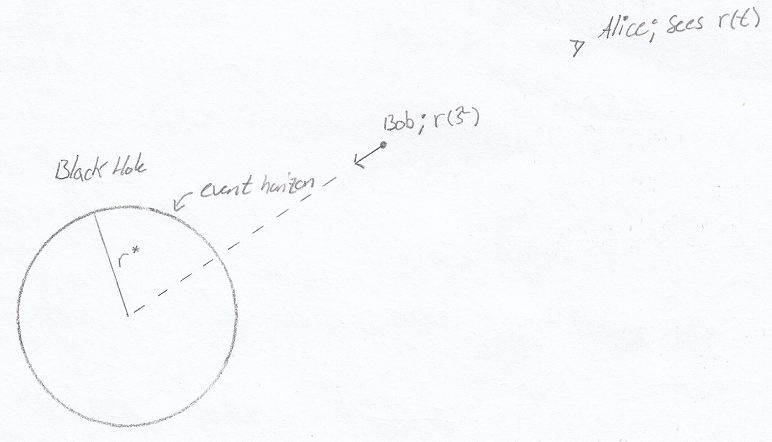
\includegraphics[width=0.8\textwidth]{figures//bh}
		\caption{The scenario with the black hole, Bob and Alice.}
		\label{fig:bh}
	\end{figure} 
	I can find $r(\tau)$ and $r(t)$ by using the variational principle. To this end I need the Lagrangian of the gravitational field. The Lagrangian is found from the metric, cf. equation \eqref{L1}, which is the Schwarzschild metric. The Schwarzschild metric describes the gravitational field from a spherically symmetric source, eg. a planet, star, black holes,.... It is given by
	\begin{equation}
		ds^2=-f(r)dt^2+f(r)^{-1}dr^2+r^2d\Omega^2,
	\end{equation} 
	where
	\begin{equation}
		f(r)=1-\frac{2MG}{r}.
	\end{equation}  
	Hereby the Lagrangian can be determined
	\begin{equation}
		L=-f(r)\dot{t}^2+f(r)^{-1}\dot{r}^2+r^2\dot{\theta}^2+r^2sin(\theta)^2\dot{\varphi}^2=-1.
	\end{equation} 
	Since I take Bob to fall in radially; $\dot{\varphi}=\dot{\theta}=0$. Hereby
	\begin{equation}
		L=-f(r)\dot{t}^2+f(r)^{-1}\dot{r}^2=-1.
	\end{equation} 
	From the Lagrangian I can determine the EOM of $t,r$ via the Euler-Lagrange equation. However, in this any most other cases, it is easier to combine the use of EOM's from the Euler-Lagrange equation and $L=-1$ - this last property is unique to GR. In this case it is (seen in hindsight) wise to begin with the EOM for the time-component
	\begin{equation}
		\frac{\partial L}{\partial t}-\frac{d}{d\tau}\bigg(\frac{\partial L}{\partial \dot{t}}\bigg)=0\Rightarrow \frac{d}{d\tau}\bigg(\underbrace{f(r)\dot{t}}_{\equiv \tilde{L}}\bigg)=0.
	\end{equation} 
	From the above I can determine $\dot{t}^2$ and insert it in $L$. Hereby
	\begin{equation}
		\tilde{L}^2-\dot{r}^2=f(r).
	\end{equation} 
	To solve this equation, I use that $L=const$ and that it can be evaluated in the limit of $r\Rightarrow\infty$. In this limit $f(r)\Rightarrow 1$ and $\dot{t}\Rightarrow1$, and so $\tilde{L}=1$. Hereby
	\begin{equation}
		\tilde{L}^2-\dot{r}^2=f(r)\Rightarrow \frac{dr}{d\tau}=-\sqrt{\frac{2MG}{r}},
	\end{equation} 
	where the minus sign comes from the fact that Bob is falling into the black hole - so it is directional. From the above I find via separation of variables
	\begin{equation}
		\sqrt{r}dr=-\sqrt{2MG}d\tau\Rightarrow r(\tau)\propto \tau^{\frac{2}{3}}.
	\end{equation} 
	The prefactor of $r(\tau)$ is not important in this case. What is important is the fact that there is no singularity at the event horizon. Bob experience himself falling through the event horizon without any changes. The question is now whether Alice will agree with Bob! To find $r(t)$ I use that
	\begin{equation}
		\frac{dr}{dt}=\frac{\dot{r}}{\dot{t}}=-\sqrt{\frac{2MG}{r}}\bigg(1-\frac{2MG}{r}\bigg).
	\end{equation} 
	In the limit of $r\Rightarrow 2MG$ the above differential equation has a solution on the form\footnote{Found by Taylor-expanding around $r=2MG$.}
	\begin{equation}
		r\approx 2MG+const\cdot e^{-\frac{t}{2MG}}.
	\end{equation} 
	What is noteworthy here is that as $t\Rightarrow \infty$ Alice will see Bob approach $r=2MG$, but never cross it! Hence, Bob and Alice will disagree on what transpires. This disagreement is due to time-dilation. 
\end{example}

\section{The Einstein equation}
The Einstein equation\index{Einstein equation} is the equation of motion for the metric, i.e. the gravitational field. The derivation of the Einstein equation revolves around the generalization of the classical equation that relates the gravitational field to the mass distribution; i.e. the Poisson equation
\begin{equation}
	\nabla^2\phi=4\pi G_N\rho.
\end{equation} 
In the relativistic limit the gravitational field and mass-energy is represented by the metric and energy-momentum tensor, respectively. Therefore, the starting point is an equation on the form
\begin{equation}
	f(g_{\mu\nu})=g(T_{\mu\nu}),
\end{equation} 
where $f$ and $g$ are \emph{some} functions of the metric and the (symmetric) energy-momentum tensor, respectively. Because $T^{00}=\rho$; $g\propto T_{\mu\nu}$. As for $f$; because of the classical limit it is expected that $f\supset \partial^2g^{\mu\nu}$. Further more, since the gravitational field can store energy, it is expected that field strength terms are included in $f$, i.e. $f\supset (\partial g_{\mu\nu})^2$. To be even more specific use that the mass-energy distribution curves space-time, so it is expected that $f$ is related to curvature. The curvature is measured by the Riemann curvature tensor that is defined in terms of the commutator of the covariant derivatives
\begin{equation}
	[D_\mu,D_\nu]V_\alpha\equiv R^\sigma_{\,\,\,\mu\beta\alpha}V_\sigma,
\end{equation} 
where
\begin{equation}
	R^{\sigma}_{\,\,\,\, \alpha \mu\beta}=\frac{\partial \Gamma^{\sigma}_{\alpha\mu}}{\partial x^{\beta}}-\frac{\partial \Gamma^{\sigma}_{\alpha\beta}}{\partial x^{\mu}}+\Gamma^{\eta}_{\alpha\mu}\Gamma^{\sigma}_{\beta\eta}-\Gamma^{\eta}_{\alpha\beta}\Gamma^{\sigma}_{\mu\eta}.
\end{equation} 
Because of Lorentz covariance $f$ cannot be directly proportional to $R^{\sigma}_{\,\,\,\, \alpha \mu\beta}$. Instead $f\sim g_{\sigma\mu}R^{\sigma}_{\,\,\,\, \alpha \mu\beta}=R^{\mu}_{\,\,\,\, \alpha \mu\beta}$ - where $R^{\mu}_{\,\,\,\, \alpha \mu\beta}=R_{\alpha\beta}$ is called the Ricci tensor. Therefore, a first guess about the form of the Einstein equation is
\begin{equation}
	R^{\mu}_{\,\,\,\, \alpha \mu\beta}\sim T_{\alpha\beta}.
\end{equation} 
However, as will be shown later on, the energy momentum tensor is the conserved Noether current associated with space-time translations in SR. This means\footnote{$,\mu$ denotes a partial derivative w.r.t. $\mu$. $;\mu$ denotes a covariant derivative w.r.t. $\mu$.}
\begin{equation}
	\text{SR:   }T^{\mu\nu}_{\,\,\,\,\,\,\, ,\mu}=0\Rightarrow \text{GR:   }T^{\mu\nu}_{\,\,\,\,\,\,\, ;\mu}=0.
\end{equation} 
This means that the covariant derivative of the Einstein equation should vanish. However, $R^{\mu\nu}_{\,\,\,\,\,\,\, ;\mu}\neq 0$, so $R^{\mu\nu}\propto T^{\mu\nu}$ is not the form of the Einstein equation. However, $f$ should still be related to the curvature in the form of the Ricci tensor. This conundrum is fixed by evaluating the covariant derivative of the Ricci tensor and subtracting the result - hence, a quantity related to the curvature will with a vanishing covariant derivative is obtained. The covariant derivative of the Ricci tensor can be evaluated by brute force, however this approach is a bit tedious since the Ricci tensor has four terms and the covariant derivative has three terms (an extra term since the covariant derivative is of a tensor with two indices). Instead use the Bianchi identity
\begin{equation}
	R_{\alpha\mu\nu\beta;\eta}+R_{\alpha\mu\eta\nu;\beta}+R_{\alpha\mu\beta\eta;\nu}=0.
\end{equation}  
Multiply this with $g^{\alpha\nu}$ and use that the covariant derivative of the metric vanishes. Hereby the metric can be pulled inside the covariant derivative to act on the Riemann curvature tensor. The result is given by
\begin{equation}
	R_{\mu\beta;\eta}-R_{\mu\eta;\beta}+R^\nu_{\,\,\,\mu\beta\eta;\nu}=0.
\end{equation}  
where the minus sign comes from permuting the outer indices of the Riemann curvature tensor. Multiplying once more with $g^{\mu\beta}$
\begin{equation}
	R_{;\eta}-R^ \beta_{\,\,\,\eta;\beta}-R^\nu_{\,\,\,\eta;\nu}=0.
\end{equation}  
Factorizing the covariant derivative and rewriting a bit
\begin{equation}
	\bigg(\frac{1}{2}\delta^\beta_{\,\,\,\eta}R-R^{\beta}_{\,\,\,\eta}\bigg)_;=0 \leftrightarrow \bigg(R^{\mu\nu}-\frac{1}{2}g^{\mu\nu}R\bigg)_;=0,
\end{equation}  
where $R$ is the Ricci scalar - the contracted version of the Ricci tensor. The last equality is what is needed for the Einstein equation! Therefore
\begin{equation}
	R^{\mu\nu}-\frac{1}{2}g^{\mu\nu}R\propto T^{\mu\nu},
\end{equation}  
where the LHS is defined as the Einstein tensor
\begin{equation}
	G^{\mu\nu}\equiv R^{\mu\nu}-\frac{1}{2}g^{\mu\nu}R.
	\label{ein1}
\end{equation} 
The proportionality constant can be found from the classical limit\footnote{Be careful here since there is a little conversion from $\phi$ to $g^{00}$ - As it turns out to be. See \citet{Cheng}.}. Hereby the Einstein equation is written as
\begin{equation}
	G^{\mu\nu}=-8\pi G_NT^{\mu\nu},
	\label{Einstein}
\end{equation} 
where the minus sign comes from the definition of the Ricci tensor. The Einstein equation, as it stands in equation \eqref{Einstein}, is however not completely generic, since the constraint that the LHS only contain second derivatives is a bit too strong. Higher derivatives would be suppressed too much, but a term proportional to the metric would be allowed as long as it vanishes in the classical limit. So, in the most generic form, to second order in the derivatives, the Einstein equation is given by
\begin{equation}
	G^{\mu\nu}+g^{\mu\nu}\Lambda=-8\pi G_NT^{\mu\nu}.
	\label{Einstein1}
\end{equation} 
$\Lambda$ is called the cosmological constant and it can be interpreted as a vacuum energy if it is moved to the RHS and taken as a contribution to the energy-momentum tensor. 
Equation \eqref{Einstein1} is the end product; it is the Einstein equation in its final form. The Einstein equation can be used to obtain the gravitational field from a given mass-energy distribution. The gravitational field can then be used in the geodesic equation to obtain the trajectories of particles in free fall in the gravitational field.  

\section{Standard Cosmology}
\label{SC}
\index{Standard cosmology}
The standard model of cosmology is built upon the FRW metric and the Friedmann equations derives therefrom. The FRW metric describes the gravitational field on cosmological scales, that is it describes the evolution of the universe as a whole. It is built from what is called the cosmological principle which approximates the universe as a perfect, spatially homogeneous, isotropic, fluid, as seen from the reference frame of a comoving observer\footnote{A comoving observer is one which is in free-fall in space-time, and for which the proper time is equal to the coordinate time, ie $g_{00}=-1$.}, on very large scales. The particles in the perfect fluid are taken to be the gravitationally bound objects in the universe. From these assumptions the metric is developed by writing down the most generic metric and then applying the physics of the cosmological principle to simplify the metric. \newline 
In general the metric depends on the choice of reference system. Taking the reference frame of the comoving observer the universe is approximated as isotropic. Since an isotropic universe has spherical symmetry the metric will be diagonal in these coordinates. Lastly, the homogeneous condition can be enforced in order to find~\citep{Weinberg1972}
\begin{equation}
	ds^2=-dt^2+R(t)^2\bigg[\frac{dr^2}{1-kr^2}+r^2d\Omega^2\bigg],
	\label{FRW}
\end{equation}  
where $d\Omega\equiv r^2d\theta^2+r^2sin(\theta)^2d\phi^2$, $r,\theta,\phi, t$ denotes radial coordinate, polar angle, azimuthal angle and time coordinate, respectively, $R(t)$ is a time-varying function called the scale factor and $k$ is a constant which sign is related to the curvature of the universe. To see how, consider different characteristics for $k, R(t)$:
\begin{enumerate}
	\item $k=0, R(t)=const\Rightarrow ds^2=-dt^2+R^2(dr^2+r^2d\Omega^2)$. Since $R=const$ it can be transformed away by a suitable coordinate transformation and the metric will thereby reduce to the Minkowski metric. The Minkowski metric results in a vanishing Riemann curvature tensor so, cf. Einsteins equation, the energy-momentum tensor will likewise vanish and there will be no matter in the universe. Hence, this is the case of an empty universe.
	
	\item $k=0, R(t)\neq const\Rightarrow ds^2=-dt^2+R^2(t)(dr^2+r^2d\Omega^2)$. Here $R(t)$ cannot be transformed away by a coordinate transformation, and even though the spatial part of the metric is flat, space-time is curved. Hence, the curvature tensor does not vanish, and the universe is not empty in this case. From observations $k\simeq 0$ and so this is a good approximation of the universe.
	
	\item $k>0, R(t)\neq const\Rightarrow ds^2=-dt^2+R(t)^2(\frac{dr^2}{1-|k|r^2}+r^2d\Omega^2)$. Once more $R(t)$ cannot be transformed away and space has a positive curvature. The spatial part of the metric resembles that of a 3D hypersphere. Since the hypersphere has a finite surface area, this universe is classified as a closed universe - referring to the finite size of the universe.
	
	\item $k<0, R(t)\neq const\Rightarrow ds^2=-dt^2+R(t)^2(\frac{dr^2}{1+|k|r^2}+r^2d\Omega^2)$. Here the spatial part of the metric resembles that of a 3D pseudo hypersphere. Since the pseudo hypersphere has infinite volume, the universe is classified as open - referring to the infinite size of the universe.
	
\end{enumerate}
By using the metric in the Einstein equation the Friedmann equations can be found. Neglecting the vacuum energy, equation \eqref{ein1} and \eqref{Einstein} can be combined to write the Einstein equation as follows
\begin{equation}
	R^{\mu\nu}-\frac{1}{2}g^{\mu\nu}R=-8\pi G_NT^{\mu\nu}.
	\label{E1}
\end{equation} 
Because the Ricci tensor includes a lot of terms the Einstein equation is often rewritten by eliminating Ricci scalar and instead introducing the trace of the energy-momentum tensor. This is done by taking the trace on both sides of equation \eqref{E1}. Hereby
\begin{equation}
	R^{\mu\nu}=-8\pi G_N(T^{\mu\nu}-\frac{1}{2}g^{\mu\nu}T^{\alpha}_{\,\,\,\alpha}).
	\label{E2}
\end{equation}  
To obtain the equations for $R(t)$ use equation \eqref{FRW} in equation \eqref{E2} to determine the Ricci tensor and use that the energy-momentum tensor for a perfect fluid is given by
\begin{equation}
	T^{\mu\nu}=Pg^{\mu\nu}+(P+\rho)u^\mu u^\nu,
\end{equation} 
where $P$ is the pressure of the fluid, $\rho$ is the energy density of the fluid and $u$ is the four-velocity. The energy-momentum tensor is the conserved Noether current associated with space-time translations in Sr. Therefore the relativistic divergence of the energy-momentum tensor must vanish in SR. Generalizing from SR to GR the derivative is generalized to th covariant derivative. Therefore
\begin{equation}
	T^{\mu\nu}_{\,\,\,\,\,\, ; \nu}=0.
	\label{T1}
\end{equation} 
The $\mu=0$ component of equation \eqref{T1} reveals
\begin{equation}
	d(\rho R^3)=-Pd(R^3)\rightleftarrows \dot{\rho}+3H(\rho +P)=0,
	\label{T2}
\end{equation}  
where $H\equiv \frac{\dot{R}}{R}$. Equation \eqref{T2} implies that the expansion of the universe can leads to local changes in the energy density. Note that the space-time geometry can hold energy and so energy can flow between it and matter - hence the energy of the space-time geometry has to be counted if one is to consider energy conservation. Taking $E=\rho V$ and $R^3\sim V$ equation \eqref{T2} can be rewritten as follows
\begin{equation}
	dE+pdV=0.
	\label{E3}
\end{equation} 
Equation \eqref{E3} is the first law of thermodynamics with no heat exchange ($dQ=0$). Hence, cf. equation \eqref{E3}, the FRW metric implies that the universe expands adiabatically ($dQ=0$). Approximating the processes that occur to be reversible means the expansion is also isentropic, i.e.$dQ_{rev}=TdS=0\Rightarrow dS=0$. The approximation of reversible processes is equivalent to the approximation of local thermal equilibrium in the universe. It is important to emphasize this approximation since it is key in the established formalism that treats DM.\newline
Using $P=w\rho$ with $w=const$ in equation \eqref{T2} reveals $\rho\propto R^{-3(1+w)}$. $w$ depends on which component dominates the universe. The popular considerations are radiation ($w=\frac{1}{3}$), matter ($w=0$) and vacuum energy ($w=-1$)
\begin{equation}
	\begin{split}
		\text{Radiation:} \quad &\rho\propto R^{-4},\\
		\text{Matter:} \quad &\rho\propto R^{-3},\\
		\text{Vacuum energy:} \quad &\rho=const.\\
	\end{split}
\end{equation}  
In this thesis the early universe, which was radiation dominated, will primarily be considered and so $\rho\propto R^{-3}$ will often be assumed. By evaluating the different components of equation \eqref{E2}; One from the $00$-component and one from the $ij$-components
\begin{equation}
	\bigg(\frac{\dot{R}}{R}\bigg)^2\equiv H^2=\frac{8\pi G_N}{3}\rho-\frac{k}{R^2}, \qquad \frac{\ddot{R}}{R}=-\frac{4\pi G_N}{3}(\rho+3P).
	\label{fried}
\end{equation} 
Equation \eqref{fried} defines the Friedmann equations (the first to the left) which describe the relationship between curvature, matter density, pressure and the expansion of the universe. The first Friedmann equation is often rewritten by defining $\rho_c\equiv \frac{3H^2}{8\pi G_N}$. Hereby
\begin{equation}
	H^2=\frac{8\pi G_N}{3}\rho-\frac{k}{R^2}\Rightarrow \frac{k}{H^2R^2}=\Omega-1,
	\label{f1}
\end{equation} 
where $\Omega\equiv \frac{\rho}{\rho_c}$. Since $k\simeq 0$ is observed it is clear from equation \eqref{f1} that $\Omega\simeq 1$.
	
	\part{Quantum Field Theory applied to particle physics}
	\chapter*{Introduction}
Elementary particle physics is the area of physics concerning the behavior of the elementary particles. An elementary particle is a particle that is assumed not to consist of any smaller particles. Hence, the proton (which consists of quarks) is not an elementary particle whereas the quarks are (since these are assumed not to be "separable"). Elementary particle physics are used in several ways and has several faces; one area of physics in which elementary particle physics are used is nuclear physics. Nuclear physics considers the interaction between particles that can be observed in the lab\footnote{Protons, neutrons, muons, electrons... The quarks go together to form particles and the leptons exist for themselves. Hence nuclear physics consider the interaction between such particles.} in the non-relativistic limit. In the non-relativistic limit the elementary particles are confined in larger particles, and so the work with elementary particles are only indirectly. To examine the elementary particles themselves the larger particles need to be split apart. This is done by smashing the particles together at high velocities. Hence, the real at which elementary particle are examined is the relativistic limit. Since the elementary particles are quantum particles the proper formalism to describe elementary particles is quantum field theory (QFT).
QFT is a versatile theoretical construct that can be used in several areas of physics. In this chapter I will focus on how it can be used to describe the elementary particles that appear in the standard model. 

\chapter{Lagrangian Density of the SM}
The SM is the theory that describes the physics of elementary particles. The elementary particles of the SM can be grouped as follows
\begin{equation}
	\left.
	\begin{cases}
		Quarks\\
		Leptons\\
	\end{cases}\right \}\Rightarrow \text{Fermions, spin}\frac{1}{2}\Rightarrow\text{Makes up the "matter".}
\end{equation} 
\begin{equation}
	\left.
	\begin{cases}
		g & \\
		W^{\pm}, Z^0 \\
		\gamma & \\
	\end{cases}\right \}\Rightarrow \text{Vector bosons, spin 1}\Rightarrow \text{Makes up "interactions".}
\end{equation} 
\begin{equation}
	\left.
	\begin{cases}
		Higgs\\
	\end{cases}\right \}\Rightarrow \text{Scalar, spin 0}\Rightarrow\text{Gives mass to the fermions and } W^{\pm}, Z^0 \text{bosons.}
\end{equation} 
where there are 8 gluons which mediates strong interaction and couples to quarks, the $W^{\pm}, Z^0$ bosons mediate the weak interaction and couples to quarks and leptons and the photon mediates EM interaction and couples to charged particles. These are the SM particles. The relevant theoretical construction used to describe the SM particles is QFT. In QFT particles are interpreted as excitations in fields, so to each particle corresponds one quantum field. The quantum fields are in turn described in terms of a Lagrangian density. Based on the particle content of the SM one therefore expects a Lagrangian density on the form
\begin{equation}
	\mathcal{L}_{sm}\sim \mathcal{L}_{fermions}+\mathcal{L}_{vb}+\mathcal{L}_{Higgs},
	\label{SM lag}
\end{equation} 
where vb abbreviates "vector bosons". Since one field is needed to describe each type of particle it is expected that three types of fields are needed; scalar fields, Dirac (spin $\frac{1}{2}$) fields and vector fields (spin $1$). This is however not completely correct; \emph{four} types of fields are actually needed, since the vector fields come in two forms: Abelian and non-abelian. Further more, it is expected that, since the particles can interact, the Lagrangian density will contain all sorts of interaction terms. These interaction terms can be deduced after introducing the free fields (scalar, Dirac and abelian gauge fields) and the non-abelian gauge fields. The free field theories are defined as the ones which are given in terms of classical Lagrangian density that can be quantized via \emph{canonical quantization}. 

\section{Canonical Quantization}
Canonical quantization is a method for turning a non-interacting, classical field into a free quantum field, and as such it defines what is meant by a "free quantum field". The free field theories considered are those relevant for the standard model of elementary particle physics (SM); the free scalar field, the free Dirac field and the free photon field.
So, the first questions one might ask is; what is the goal of quantization? When is the quantization process completed? Since free field theories are considered, the particles they represent cannot interact and all they do is propagate. Therefore, all the information from the free field theory is contained in the probability amplitude for a particle to be created at one point and annihilated at another point - this probability amplitude is defined as the propagator. In terms of fields it is given by
\begin{equation}
	G\equiv\braket{0|T\{\text{fields}\}|0},
	\label{prop def}
\end{equation} 
where $G$ denotes that the propagator is a two-point Greens function and $T\{\dots\}$ denotes the act of time ordering, i.e. the ordering of the fields with the "latest" time to the left. Since the propagator depends on the fields, there is a different propagator to each free field.

\subsection*{The free, real scalar field}
The first free field considered is the free, real scalar field\footnote{The field is specified to be real because the free, complex scalar field is another field.}. The real scalar field is the simplest field and so it works well to illustrate the procedure of canonical quantization. The procedure follows five steps:
\begin{enumerate}
	\item Write up the classical Lagrangian density in terms of the field in question:
	\begin{equation}
		\mathcal{L}=\frac{1}{2}\partial_\mu\phi\partial^\mu\phi-\frac{1}{2}m^2\phi^2.
		\label{Lagrange scalar}
	\end{equation} 
	From the Lagrangian density find the equation of motion (EOM) via using the Euler-Lagrange equation
	\begin{equation}
		\frac{\partial \mathcal{L}}{\partial \phi}-\partial_\mu\frac{\partial \mathcal{L}}{\partial (\partial_\mu\phi)}=0\Rightarrow (\square+m^2)\phi=0,
	\end{equation} 
	where $\square=\partial_\mu\partial^\mu$. This particular EOM is called the Klein-Gordon (KG) equation.
	
	\item The solution to the KG equation is on the form of a plane wave, i.e. $\phi(x)\sim e^{\pm ip\cdot x}$. After quantization is complete the solution with a plus sign represents a particle with negative energy, i.e. an anti-particle. However, for the real scalar field the particle is its own anti-particle, so this aspect does not come into play here - it will however do so for the Dirac field. Because the solution is on the form of a plane wave, the solution (field) can be expanded in what is called a plane wave expansion cf.
	\begin{equation}
		\phi(x)=\int \frac{d^3 p}{(2\pi)^3}\frac{1}{\sqrt{2E_{\vec{p}}}}\bigg(a_{\vec{p}}\,e^{-ip\cdot x}+a_{\vec{p}}^*\,e^{ip\cdot x}\bigg),
		\label{phi}
	\end{equation} 
	where the factor of $\frac{1}{\sqrt{2E_{\vec{p}}}}$ is there to ensure Lorentz invariance of the integration measure and $E_{\vec{p}}^2=\vec{p}\,^2+m^2$. The field in equation \eqref{phi} is still a classical field. Note that the field is a function of space-time and when quantized it will therefore be represented in the Heisenberg scheme - since the field is the dynamical variable in QFT, taking the place of position in QM, and time-dependent dynamical variables belong in the Heisenberg scheme. 
	
	\item Calculate the momentum conjugate to the field via
	\begin{equation}
		\begin{split}
			\Pi(x)&\equiv \frac{\partial \mathcal{L}}{\partial (\partial_0\phi)}\\
			&=\partial_0\phi\\
			&=\int \frac{d^3 p}{(2\pi)^3}\frac{(-iE_{\vec{p}})}{\sqrt{2E_{\vec{p}}}}(a_{\vec{p}}\,e^{ip\cdot x}-a_{\vec{p}}^*\,e^{-ip\cdot x}).
		\end{split}
	\end{equation} 
	
	\item Promote the classical fields ($\phi$ and $\Pi$) to operator valued quantum fields. This is done by promoting the expansion coefficients ($a_{\vec{p}}$ and $a_{\vec{p}}^*$) to ladder operators. Subsequently to the promotion, impose the canonical commutator relations
	\begin{equation}
		[\phi(\vec{x},t),\Pi(\vec{y},t)]=i\delta^{(3)}(\vec{x}-\vec{y}),\quad [\phi(\vec{x},t),\phi(\vec{y},t)]=[\Pi(\vec{x},t),\Pi(\vec{y},t)]=0.
	\end{equation} 
	These commutator relations are called equal time commutator relations. The commutator relations will impose commutator relations on the coefficients. If these can be imposed without violating any physical principles, then the theory is quantized. In the case of the real scalar field the commutator relations of the fields imposes on the coefficients
	\begin{equation}
		[a_{\vec{p}},a_{\vec{q}}^\dagger]=(2\pi)^3\delta^{(3)}(\vec{p-\vec{q}}), \quad [a_{\vec{p}},a_{\vec{q}}]=[a_{\vec{p}}^\dagger,a_{\vec{q}}^\dagger]=0.
	\end{equation} 
	These commutator relations are the relations of the ladder operators. The quantized field is to be understood in terms of its effect on the vacuum state
	\begin{equation}
		\begin{split}
			\phi(x)\ket{0}&=\int \frac{d^3p}{(2\pi)^3}\frac{1}{\sqrt{2E_{\vec{p}}}} e^{-ip\cdot x}\ket{\vec{p}}\\
			&=\text{Linear superposition of single particle states with well-defined momentum.}.\\
		\end{split}
	\end{equation} 
	The above is interpreted as follows $\phi(x)$ acting on the vacuum creates a particle at space-time point $x$. In general, $\phi(x)$ acting on a generic state, can create and/or annihilate particles at a given space-time position.
	\item Determine the propagator of the free theory. The propagator of the free theory can be found by using the definition
	\begin{equation}
		D_F(x-y)=\braket{0|T\{\phi(x)\phi(y)\}|0},
	\end{equation} 
	where $D_F(x-y)$ is used instead of $G$ to denote that it is the propagator for the real scalar field. The propagator is both defined in real space and momentum space. The real space representation is found by insertion of the field into the definition,  i.e.
	 \begin{equation}
		\begin{split}
			D_F(x-y)&=\braket{0|T\{\phi(x)\phi(y)\}|0}\\
			&=\braket{0|\int \frac{d^3 p}{(2\pi)^3}\frac{1}{\sqrt{2E_{\vec{p}}}}\bigg(a_{\vec{p}}\,e^{-ip\cdot x}+a_{\vec{p}}^\dagger\,e^{ip\cdot x}\bigg)\int \frac{d^3 q}{(2\pi)^3}\frac{1}{\sqrt{2E_{\vec{q}}}}\bigg(a_{\vec{q}}\,e^{-iq\cdot y}+a_{\vec{q}}^\dagger\,e^{iq\cdot y}\bigg)|0}.\\
		\end{split}
	\end{equation} 
	The above will have four different terms with ladder operators
	\begin{equation}
		\braket{0|a_{\vec{p}},a_{\vec{q}}|0}=\braket{0|a_{\vec{p}}^\dagger,a_{\vec{q}}|0}=\braket{0|a_{\vec{p}}^\dagger,a_{\vec{q}}^\dagger|0}=0,
	\end{equation} 
	\begin{equation}
		\begin{split}
			\braket{0|a_{\vec{p}},a_{\vec{q}}^\dagger|0}&=\braket{0|a_{\vec{q}}^\dagger,a_{\vec{p}}|0}+\braket{0|0}(2\pi)^3\delta^{(3)}(\vec{p}-\vec{q})\\
			&=(2\pi)^3\delta^{(3)}(\vec{p}-\vec{q}).
		\end{split}
	\end{equation} 
	Hereby
	\begin{equation}
		\begin{split}
			D_F(x-y)&=\int \frac{d^3 p}{(2\pi)^3}\int \frac{d^3 q}{(2\pi)^3}\frac{1}{\sqrt{2E_{\vec{p}}}}\frac{1}{\sqrt{2E_{\vec{q}}}}(2\pi)^3\delta^{(3)}(\vec{p}-\vec{q})e^{-i(p\cdot x-q\cdot y)}\\
			&=\int \frac{d^3 p}{(2\pi)^3}\frac{1}{2E_{\vec{p}}}e^{-i(p\cdot x-q\cdot y)}.
			\label{prop1}
		\end{split}
	\end{equation} 
	This is the propagator of the free, real scalar field in the position representation. Most often, however, the propagator is used in the momentum representation. This can be found by using that the free, real scalar field obeys the Klein-Gordon equation. Consequently the propagator is the Greens function of the the Klein-Gordon equation,  i.e.
	\begin{equation}
		(\square+m^2)D_F(x-y)=-i\delta^{(4)}(x-y).
		\label{prop}
	\end{equation} 
	Equation \eqref{prop} can be used to find the momentum, and position, representation of the propagator by expressing the propagator in terms of the inverse Fourier transform of the momentum representation
	\begin{equation}
		D_F(x-y)=\int \frac{d^4p}{(2\pi)^4}e^{-ip\cdot(x-y)}\tilde{D}_F(p).
		\label{fourier1}
	\end{equation} 
	By using this
	\begin{equation}
		\begin{split}
			(\square+m^2)D_F(x-y)&=\int\frac{d^4p}{(2\pi)^4}(-p^2+m^2)\tilde{D}_F(p)e^{-ip\cdot(x-y)}\\
			&=-i\delta^{(4)}(x-y).
		\end{split}
	\end{equation} 
	Now, since\index{Fourier transform, delta function} $\int \frac{d^4p}{(2\pi)^4}e^{-ip\cdot(x-y)}=\delta^{(4)}(x-y)$ the momentum representation of the propagator must be given by
	\begin{equation}
		\tilde{D}_F(p)=\frac{i}{p^2-m^2}.
	\end{equation} 
	Using this propagator in the Fourier expansion (equation \eqref{fourier1}) will result in an expression quite similar to equation \eqref{prop1}. However, note that there are small differences, among them the dimensionality of the integral.
\end{enumerate}

\subsection*{The Dirac field}
The next field subject to canonical quantization is the Dirac field. The five steps are repeated:
\begin{enumerate}
	\item The classical Lagrangian density in terms of the field(s) in question
	\begin{equation}
		\mathcal{L}=\bar{\psi}(i\slashed \partial-m)\psi,
	\end{equation} 
	where $\slashed \partial =\gamma^\mu\partial_\mu$ and $\gamma^\mu$ are $4\times 4$ matrices. From the Lagrangian density the EOM is found via using the Euler-Lagrange equation for $\bar{\psi}$
	\begin{equation}
		\frac{\partial \mathcal{L}}{\partial \bar{\psi}}-\partial_\alpha\frac{\partial \mathcal{L}}{\partial (\partial_\alpha \bar{\psi})}=0 \Rightarrow (i\slashed \partial -m)\psi=0.
	\end{equation} 
	This EOM is called the Dirac equation. 
	
	\item The solution to the Dirac equation is a somewhat more involved compared to the KG equation. Firstly, as indicated by the gamma-matrices which are $4\times 4$, the solutions to the Dirac equation are $4\times 1$ objects called spinors, or Dirac spinors. These can be written as
	\begin{equation}
		\psi=\begin{bmatrix}
			\psi_1\\
			\psi_2\\
			\psi_3\\
			\psi_4\\
		\end{bmatrix}=\begin{bmatrix}
		\psi_L\\
		\psi_R
	\end{bmatrix},
\end{equation} 
where $\psi_L$ and $\psi_R$ are called left-handed and right-handed Weyl spinors. A spinor differs from a vector in the way it transforms. Each component of the Dirac spinor must fulfill the KG equation, since
\begin{equation}
	(i\slashed \partial+m)(i\slashed \partial -m)\psi=-(\square+m^2)\psi=0.
\end{equation} 
Hence, the solution must once again be on the form of a plane wave, i.e. $\psi(x)\sim e^{\pm ip\cdot x}$. However, in the case of the Dirac field, which is not required to be real, the two sets of solutions will result in a particle and an anti-particle. Further more, since the solution must fulfill the Dirac equation, but have the position dependence such that it fulfills the KG equation, the solutions are parametrized cf.
\begin{equation}
	\psi(x)=u(\vec{p}\,)e^{-ip\cdot x}=\begin{bmatrix}
		u_L(\vec{p}\,) \\u_R(\vec{p}\,)\\
	\end{bmatrix}e^{-ip\cdot x}, \quad \psi(x)=v(\vec{p}\,)e^{ip\cdot x}=\begin{bmatrix}
	v_L(\vec{p}\,)\\
	v_R(\vec{p}\,)\\
\end{bmatrix}e^{ip\cdot x}.
\end{equation} 
The functions $u(\vec{p}\,)$ and $v(\vec{p}\,)$ satisfy the Dirac equations in momentum space. These are found by inserting the parametrized solutions into the Dirac equation
\begin{equation}
	(\slashed p-m)u(\vec{p}\,)=0, \quad (-\slashed p-m)v(\vec{p}\,)=0.
	\label{orse}
\end{equation} 
To determine the functions $u(\vec{p}\,)$, $v(\vec{p}\,)$ the solution is considered in the reference frame at which the particle is at rest, and thereafter the solution can be boosted to an arbitrary reference frame. In the rest frame; $\vec{p}_{rf}^T=\begin{bmatrix}
m &
\vec{0}\\
\end{bmatrix}$ and so
\begin{equation}
	\begin{split}
		(\gamma^0 m -m)u(\vec{p}_{rf})&=\begin{bmatrix}
			-m & m \\
			m & -m \\
		\end{bmatrix}\begin{bmatrix}
		u_L(\vec{p}_{rf})\\
		u_R(\vec{p}_{rf})\\
	\end{bmatrix}=\begin{bmatrix}
	0\\
	0\\
\end{bmatrix}\\
&\Rightarrow u_L(\vec{p}_{rf})=u_R(\vec{p}_{rf})\equiv\xi^s\\
&\Rightarrow u(\vec{p}_{rf})=\sqrt{m}\begin{bmatrix}
	\xi^s\\
	\xi^s\\
\end{bmatrix},
\end{split}
\end{equation} 
where $\sqrt{m}$ is included by convention, $\xi^s$ is a two component spinor that is normalized cf. $\xi\xi^\dagger=1$, and $s=1,2$ represents the spin states (along the $z$-axis) of the particle. Likewise for $v(\vec{p})$
\begin{equation}
	\begin{split}
		(-\gamma^0 m -m)v(\vec{p}_{rf})&=\begin{bmatrix}
			-m & -m \\
			-m & -m \\
		\end{bmatrix}\begin{bmatrix}
		v_L(\vec{p}_{rf})\\
		v_R(\vec{p}_{rf})\\
	\end{bmatrix}=\begin{bmatrix}
	0\\
	0\\
\end{bmatrix}\\
&\Rightarrow v_L(\vec{p}_{rf})=-v_R(\vec{p}_{rf})\equiv\eta^s\\
&\Rightarrow v(\vec{p}_{rf})=\sqrt{m}\begin{bmatrix}
	\eta^s\\
	-\eta^s\\
\end{bmatrix}.
\end{split}
\end{equation} 
It is clear that the solutions have two free components, the components of $\xi$ and $\eta$, this is what is expected since the Dirac field describes spin $\frac{1}{2}$ particles - and spin $\frac{1}{2}$ particles only have two physical states; spin up and down. From the solutions in the rest frame of the particle the solution in a generic reference frame can be found, as mentioned, by boosting to a generic reference frame. Hereby
\begin{equation}
	u^s(\vec{p}\,)=\begin{bmatrix}
		\sqrt{p\cdot \sigma} \xi^s\\
		\sqrt{p\cdot\bar{\sigma}}\xi^s\\
	\end{bmatrix}, \quad v^s(\vec{p}\,)=\begin{bmatrix}
	\sqrt{p\cdot \sigma} \eta^s\\
	-\sqrt{p\cdot\bar{\sigma}}\eta^s\\
\end{bmatrix},
\end{equation} 
where $\sigma^T=\begin{bmatrix}
1 & \vec{\sigma}\\
\end{bmatrix}$ and $\bar{\sigma}^T=\begin{bmatrix}
1 & -\vec{\sigma}\\
\end{bmatrix}$. 
With the solutions to the Dirac equation determined the fields can be expanded in a plane-wave expansion
\begin{equation}
	\psi(x)=\int \frac{d^3p}{(2\pi)^3}\frac{1}{\sqrt{2E_{\vec{p}}}}\sum_s\bigg(a_{\vec{p},s}u^s(\vec{p}\,)e^{-ip\cdot x}+b_{\vec{p},s}^\dagger v^s(\vec{p}\,)e^{ip\cdot x}\bigg),
\end{equation} 
\begin{equation}
	\begin{split}
		\bar{\psi}(x)&\equiv\psi^\dagger\gamma^0\\
		&=\int \frac{d^3p}{(2\pi)^3}\frac{1}{\sqrt{2E_{\vec{p}}}}\sum_s\bigg(b_{\vec{p},s}\bar{v}^s(\vec{p}\,)e^{-ip\cdot x}+a_{\vec{p},s}^\dagger \bar{u}^s(\vec{p}\,)e^{ip\cdot x}\bigg),
	\end{split}
\end{equation} 
where the expansion coefficients for $v$, i.e. $b^s$, denote what is to become the ladder operators of the anti-particle. Likewise for $u$, i.e. $a^s$, are to become the ladder operators of the particle.

\item In the case of the Dirac field there is only one conjugate momentum, namely the momentum conjugate to $\psi$. This is because the conjugate momentum is proportional, cf. the definition $\Pi_i\equiv \frac{\partial \mathcal{L}}{\partial (\partial_0 \phi_i)}$, to the time-derivative of the field. From the Dirac equation is it clear that only the time-derivative of $\psi$ appears, so there is only one conjugate momentum
\begin{equation}
	\Pi=\frac{\partial \mathcal{L}}{\partial (\partial_0\psi)}=i\bar{\psi}\gamma^0=i\psi^\dagger.
\end{equation} 
\item The classical fields are promoted to operator valued quantum fields by promoting the expansion coefficients to ladder operators. Note, however, that there are now two sets; one for the particle and one for the anti-particle. Subsequently, impose the canonical commutator relations on the fields. However, now that the particles are fermions, cf. the spin statistic theorem, the commutator relations that are to be imposed are \emph{anti-commutator relations}
\begin{equation}
	\{\psi_a(\vec{x},t),\Pi_b(\vec{y},t)\}=i\{\psi_a(\vec{x},t),\psi^\dagger_b(\vec{y},t)\}=i\delta^{(3)}(\vec{x}-\vec{y})\delta_{ab},
\end{equation} 
\begin{equation}
	\{\psi_a(\vec{x},t),\psi_b(\vec{y},t)\}=\{\psi_a^\dagger(\vec{x},t),\psi_b^\dagger(\vec{y},t)\}=0.
\end{equation} 
These commutator relations result in commutator relations for the ladder operators
\begin{equation}
	\{a_{\vec{p}}^r,a_{\vec{q}}^{s\dagger}\}=\{b_{\vec{p}}^r,b_{\vec{q}}^{s\dagger}\}=(2\pi)^3\delta^{(3)}(\vec{p}-\vec{q})\delta_{rs},
\end{equation} 
where all other anti-commutator-combinations of the ladder operators vanish. Analogous to the interpretation of the scalar field operator; $\psi$ creates an anti-particle or destroys a particle and $\bar{\psi}$ does the opposite.

\item Determine the propagator of the free theory. For the Dirac field
\begin{equation}
	S_F(x-y)=\braket{0|T\{\psi(x)\bar{\psi}(y)\}|0}.
\end{equation} 
Once again the definitions of the fields can be used to determine the form of the propagator in position space. To determine the momentum representation use that the Dirac propagator is the Greens function of the Dirac equation, i.e.
\begin{equation}
	(i\slashed \partial-m)S_f(x-y)=i\delta^{(4)}(x-y).
\end{equation} 
The same approach as for the scalar field is used; express the field in terms of the inverse Fourier transform of the momentum representation and use it in the equation for the Greens function. The inverse Fourier transform
\begin{equation}
	S_F(x-y)=\int \frac{d^4p}{(2\pi)^3}e^{-ip\cdot(x-y)}\tilde{S}_F(p).
\end{equation} 
Inserted into the equation for the Greens function
\begin{equation}
	\begin{split}
		(i\slashed \partial-m)S_f(x-y)&=\int \frac{d^4p}{(2\pi)^3}(i\slashed p-m)e^{-ip\cdot(x-y)}\tilde{S}_F(p)\\
		&=i\delta^{(4)}(x-y).
	\end{split}
\end{equation} 
Using once more that $\int \frac{d^4p}{(2\pi)^4}e^{-ip\cdot(x-y)}=\delta^{(4)}(x-y)$ results in the propagator in momentum space
\begin{equation}
	\tilde{S}_F(p)=\frac{i}{\slashed p-m}=\frac{i(\slashed p+m)}{p^2-m^2},
\end{equation} 
where the factor of $i\varepsilon$ often is added in the denominator for computational purposes. 
\end{enumerate}

\subsection*{The EM field}
The canonical quantization of the EM field is a bit tricky because EM is an abelian gauge theory. "Abelian" refers to the fact that the generators of the group commute - in practice it means that the theory is quantized via canonical quantization (i.e. it means that the theory is free). "Gauge theory" refers to the fact that the theory may admit different configurations resulting in the same physical observables. Hence, the theory contains some inherent vagueness and so one can choose one of the many equivalent formulations. The formulations are called gauges, transformations between different formulations are called gauge transformations and the invariance of the physical theory under a gauge transformation is called gauge invariance. 
The EM theory is gauge invariant and so gives a redundant description. The problem is that only two of the four components of the vector field, $A^\mu$, are physically independent, while the theory allows for all four to be independent. To solve this problem a certain formulation (gauge) is chosen to remove the redundancy. The common choice of gauge is one of two:
\begin{enumerate}
	\item The Coulomb gauge; $A^0=0$ and $\vec{\nabla}\cdot\vec{A}=0$.\newline
	Impose the Coulomb gauge from the start. This will remove the redundancy, but since this gauge differs between $A^0$ and $\vec{A}$, explicit Lorentz covariance is lost. This will have to be recovered in the end.
	
	\item Make a "soft" Lorentz gauge choice.\newline
	Add a term to the Lagrangian density and quantize this Lagrangian density via canonical quantization. In the end impose the soft Lorentz gauge - The word "soft" is used because the Lorentz gauge, i.e. $\partial_\mu A^\mu=0$, is not used directly, but only when applied to physical states. In quantizing the EM field in this way the explicit Lorentz covariance is not lost. 
\end{enumerate}

The second approach will be employed here, i.e. the soft Lorentz gauge.
\begin{enumerate}
	\item The classical Lagrangian density in terms of the fields in question
	\begin{equation}
		\mathcal{L}=-\frac{1}{4}F^{\mu\nu}F_{\mu\nu}-\underbrace{\frac{1}{2}(\partial_\mu A^\mu)^2}_{\text{Gauge fixing term}}.
		\label{lagrange em}
	\end{equation} 
	From the Lagrangian density the EOM is found via the Euler-Lagrange equation
	\begin{equation}
		\frac{\partial \mathcal{L}}{\partial A^{\alpha}}-\partial_\beta\frac{\partial \mathcal{L}}{\partial (\partial_\beta A^\alpha)}=0\Rightarrow \square A^\alpha=0.
	\end{equation} 
	
	\item The solution to $\square A^\alpha=0$ is on the form of a plane wave. Taking the polarization into account, the field can be expanded cf.
	\begin{equation}
		A^\mu(x)=\int\frac{d^3p}{(2\pi)^3}\frac{1}{\sqrt{2E_{\vec{p}}}}\sum_{\lambda=0}^{3}\bigg(\varepsilon^\mu(\vec{p},\lambda)a_{\vec{p},\lambda}e^{-ip\cdot x}+\varepsilon^{\mu*}(\vec{p},\lambda)a_{\vec{p},\lambda}^*e^{ip\cdot x}\bigg).
	\end{equation} 
	
	\item The momentum conjugate to the field is calculated via
	\begin{equation}
		\Pi^\mu(x)=\frac{\partial \mathcal{L}}{\partial (\partial_0 A_\mu)}.
	\end{equation} 
	
	\item Again the classical fields are promoted to operator valued quantum fields by promoting the expansion coefficients to ladder operators. Subsequently, impose the canonical commutator relations, however, multiply with the metric to conserve the indices
	\begin{equation}
		[A^\mu(\vec{x},t), \Pi^\nu(\vec{y},t)]=ig^{\mu\nu}\delta^{(3)}(\vec{x}-\vec{y}), \quad [A^\mu(\vec{x},t),A^\nu(\vec{y},t)]=[\Pi^\mu(\vec{x},t),\Pi^\nu(\vec{y},t)]=0.
	\end{equation} 
	These commutator relations impose commutator relations upon the ladder operators
	\begin{equation}
		[a_{\vec{p},\lambda},a_{\vec{q},\lambda'}^\dagger]=-(2\pi)^3\delta^{(3)}(\vec{p}-\vec{q}),
	\end{equation} 
	\begin{equation}
		[a_{\vec{p},\lambda},a_{\vec{q},\lambda'}]=[a_{\vec{p},\lambda}^\dagger,a_{\vec{q},\lambda'}^\dagger]=0.
	\end{equation} 
	This is where the previous quantization procedures would move on the the propagator. In this case there remains work to be done. The metric's appearance in the commutator poses a problem since it results in a negative norm of the one-particle states ($\ket{\vec{p},t}=\sqrt{2E_{\vec{p}}}a_{\vec{p},\lambda}^\dagger\ket{0}$)
	\begin{equation}
		\braket{\vec{p},\lambda|\vec{p},\lambda}=2E_{\vec{p}}\braket{0|a_{\vec{p},\lambda}a_{\vec{p},\lambda}^\dagger|0}=2E_{\vec{p}}\braket{0|[a_{\vec{p},\lambda},a_{\vec{p},\lambda}^\dagger]|0}=-2(2\pi)^3\delta^{(3)}(0)<0.
	\end{equation}  
	Because of the negative norm of the states the normal interpretation of the norm, i.e. as a probability density, is not possible. However, the soft Lorentz gauge is yet to be imposed, and this fixes the issue. So far the theory that has been considered is not that of EM, but a theory different from EM. This is because a term has been added to the EM Lagrangian density, to fix the gauge, and this term has not been constrained to vanish. The idea is now to pick out only the part of the Fock space that are of physical meaning to EM. This is done through requiring the soft Lorentz gauge
	\begin{equation}
		\braket{\text{phys'}|\partial_\mu A^\mu|\text{phys}}=0.
	\end{equation} 
	So, rather than requiring $\partial_\mu A^\mu=0$ in the Lagrangian density, the Lorentz gauge is imposed as an operator equation on physical states. To ensure the above, split $\partial_\mu A^\mu$ into its positive and negative energy parts
	\begin{equation}
		\partial_\mu A^\mu=(\partial_\mu A^\mu)^++(\partial_\mu A^\mu)^-,
	\end{equation} 
	where
	\begin{equation}
		(\partial_\mu A^\mu)^+=-i\int \frac{d^3p}{(2\pi)^3}\frac{1}{\sqrt{2E_{\vec{p}}}}\sum_{\lambda=0}^{\lambda}p_\mu\varepsilon^\mu(\vec{p},\lambda)a_{\vec{p},\lambda}e^{-ip\cdot x},
	\end{equation} 
	\begin{equation}
		(\partial_\mu A^\mu)^-=i\int \frac{d^3p}{(2\pi)^3}\frac{1}{\sqrt{2E_{\vec{p}}}}\sum_{\lambda=0}^{\lambda}p_\mu\varepsilon^{\mu*}(\vec{p},\lambda)a_{\vec{p},\lambda}^\dagger e^{ip\cdot x}.
	\end{equation} 
	From the definitions above it is clear that $(\partial_\mu A^\mu)^-=((\partial_\mu A^\mu)^+)^\dagger$. Therefore, $\braket{\dots|\partial_\mu A^\mu|\dots}$=0 is fulfilled if only
	\begin{equation}
		(\partial_\mu A^\mu)^+\ket{\text{phys}}=0.
	\end{equation} 
	This equation is taken to define the physical subspace of the Fock space. Hereby the EM field has been quantized.
	
	\item Determine the propagator of the free theory. Once more use that the propagator is the Greens function of the EOM,  i.e.
	\begin{equation}
		\square D_F^{\mu\nu}(x-y)=ig^{\mu\nu}\delta^{(4)}(x-y).
	\end{equation} 
	The propagator is then expressed in terms of the inverse Fourier transform of the momentum representation
	\begin{equation}
		D_F^{\mu\nu}(x-y)=\int \frac{d^4p}{(2\pi)^4}e^{-ip\cdot (x-y)}\tilde{D}_F^{\mu\nu}(p).
	\end{equation} 
	By using this in the equation for the Greens function
	\begin{equation}
		\begin{split}
			D_F^{\mu\nu}(x-y)&=\int \frac{d^4p}{(2\pi)^4}(-p^2)\tilde{D}_F^{\mu\nu}(p)e^{-ip\cdot (x-y)}\\
			&=ig^{\mu\nu}\delta^{(4)}(x-y).\\
		\end{split}
	\end{equation} 
	From the above the propagator in momentum space is found (in the Lorentz gauge) to be
	\begin{equation}
		\tilde{D}_F^{\mu\nu}(p)=\frac{-ig^{\mu\nu}}{p^2}.
	\end{equation} 
	
\end{enumerate}

\section{Path Integral Quantization}		
Path integral quantization is a method for determining the propagator of a free theory - However, the method can also be used to quantize non-free (non-abelian gauge theories) theories. Path integral quantization therefore do the same job as canonical quantization. The two methods complement each other and each method have relative strengths and weaknesses; canonical quantization has a very clear physical interpretation whereas path integral quantization is applicable to a wider range of theories. Path integral quantization also has a clear analogy with statistical mechanics, and the theory is in principle non-perturbative\footnote{As opposed to perturbative theories.}, which means that non-perturbative effects can be determined via this method.
Since path integral quantization is an alternative to canonical quantization, the goal of the quantization procedure is the same; the propagator (equation \eqref{prop def}). The propagator is obtained by generalizing the path integral scheme from QM (section \ref{sec:path scheme}). In the QM path integral scheme all possible trajectories, for a single particle traveling between two space-time points, are summed over. Going to QFT the functional integral now sums over all possible field configurations that exist between two space-time points. Besides this, the coordinates are replaced by the fields and the Lagrangian for the Lagrangian density. For  the real, free scalar field
\begin{equation}
	q\Rightarrow \phi, \quad \int Dq\Rightarrow \int D\phi, \quad L\Rightarrow \int d^3x \mathcal{L}.
\end{equation} 
Hereby, by analogy
\begin{equation}
	\braket{\phi_f(\vec{x}),t_f|T\{\phi(x_1)\phi(x_2)\dots\}|\phi_i(\vec{x}),t_i}=\int D\phi\, \phi(x_1)\phi(x_2)\dots e^{iS}.
\end{equation} 
The find the n-point functions, let the states go to the vacuum state and $t_{f,i}\Rightarrow\pm\infty$. Further more, since the contributions from the bubbling of the vacuum is not of interest (in diagrams these are called bubble diagrams) the above expression is divided by a normalizing factor. The bubbling of the vacuum is contributions with no external particles. By normalizing
\begin{equation}
	\braket{\Omega|T\{O(\phi)\}|\Omega}=\lim\limits_{T\Rightarrow \infty(1-i\varepsilon)}\bigg(\frac{\int D\phi\,O(\phi) e^{iS}}{\int D\phi e^{iS}}\bigg),
\end{equation} 
where $\ket{\Omega}$ is the vacuum state of the full (possibly interacting) theory, $O(\phi)$ denotes some number of scalar fields, the fields on the LHS are operators valued fields and the fields on the RHS are classical fields. The limit is taken over a complex time, $T$. This is just a mathematical trick. I will get back to this when I do perturbation theory. The generalization is just as straightforward for the Dirac field and the EM field, the only difference being the different fields
\begin{equation}
	\braket{\Omega|T\{O(\psi)O(\bar{\psi})\}|\Omega}=\lim\limits_{T\Rightarrow \infty(1-i\varepsilon)}\bigg(\frac{\int D\psi\int D\bar{\psi}\,O(\psi)O(\bar{\psi}) e^{iS}}{\int D\phi e^{iS}}\bigg),
\end{equation} 
\begin{equation}
	\braket{\Omega|T\{O(A)\}|\Omega}=\lim\limits_{T\Rightarrow \infty(1-i\varepsilon)}\bigg(\frac{\int DA\,O(A) e^{iS}}{\int D\phi e^{iS}}\bigg),
\end{equation} 
where $DA=DA^0DA^1DA^2DA^3$ and $\psi,\bar{\psi}$ on the RHS are classical, anti-commuting fields known as Grassmann fields - these will be introduced just below in the subsection on quantizing the Dirac field via the path integral formalism. The number of fields in the above equations can be taken to be two, and the theory taken to be free, in order to obtain the propagators of the free theories. However, the expressions for the propagators are still complicated and unlike the expressions for the propagators in the momentum space that was found in canonical quantization. These expressions can be found by evaluating the path integrals, however, a more \emph{neat} procedure to determine n-point functions, valid for free/non-free theories, is obtained by introducing the \emph{generating functional} \index{Generating functional}. The generating functional is the analogous object to the partition function form statistical mechanics and the n-point functions are found by differentiating the partition function. The partition function is defined as the amplitude for a vacuum to vacuum  transition in the presence of source fields. The number of source fields will match the number of fields, so in scalar field theory there is a single source field, in Dirac theory there are two source fields and in the EM theory there are four source fields.

\subsection*{The real, free scalar field}
For the real, free scalar field the generating functional is defined as (cf. the above definition)
\begin{equation}
	\begin{split}
		Z[J]&=\frac{z[J]}{z[0]}=\frac{1}{z[0]}\int D\phi \, e^{i\int d^4x(\mathcal{L}+J\phi)},
	\end{split}
\end{equation} 
where $J$ is the source field for the scalar field theory and the Lagrangian density for a real, free scalar field is given by equation \eqref{Lagrange scalar}. The n-point functions for the real, free scalar field theory is found from the generating functional by using
\begin{equation}
	\braket{0|T\{O(\phi)\}|0}=\frac{1}{i}\frac{\delta}{\delta J(x_1)}\frac{1}{i}\frac{\delta}{\delta J(x_2)}\dots \bigg(Z[J]\bigg)\bigg|_{J=0}.
\end{equation} 
Here I will consider the propagator of the free theory, and so I will consider the two point function. To obtain a useful expression for the propagator the procedure is to use a method called "completing the square". In this method $z[J]$ is rewritten so as to factorize $z[0]$ and leave a relatively simple expression, containing the propagator, for $Z[J]$. First, I define the generating functional in terms of the free scalar field
\begin{equation}
Z[J]=\frac{1}{z[0]}\int D\phi \, e^{i\int d^4x(\frac{1}{2}\partial_\mu\phi\partial^\mu\phi-\frac{1}{2}m^2\phi^2+J\phi)}\equiv\frac{1}{z[0]}\int D\phi \, e^{I}.
\end{equation} 
The integral defined as $I$ is what must be massaged so $z[0]$ can be factorized
\begin{equation}
	\begin{split}
		I&=i\int d^4x\bigg(\frac{1}{2}\partial_\mu\phi\partial^\mu\phi-\frac{1}{2}m^2\phi^2+J\phi\bigg)\\
		&=i\int d^4x\bigg(-\frac{1}{2}\phi(\square-m^2)\phi+J\phi\bigg),\\
	\end{split}
\end{equation} 
where partial integration has been used. To introduce perform the factorization and introduce the propagator make a linear shift in the field cf.
\begin{equation}
	\phi(x)=\phi'(x)+i\int d^4y D_F(x-y)J(y).
\end{equation} 
By shifting the fields
\begin{equation}
	\begin{split}
		I&=i\int d^4x\bigg(-\frac{1}{2}\bigg(\phi'+i\int d^4y D_F(x-y)J(y)\bigg)(\square-m^2)\bigg(\phi'+i\int d^4z D_F(x-z)J(z)\bigg)\\
		&+J\bigg(\phi'+i\int d^4y D_F(x-y)J(y))\bigg)\\
		&=i\int d^4x\bigg(-\frac{1}{2}\phi'(\square-m^2)\phi'+J\phi'+i\int d^4yJ(x) D_F(x-y)J(y)\\
		&-\frac{1}{2}i\int d^4y D_F(x-y)J(y)(\square-m^2)\phi'-\frac{1}{2}\phi'(\square-m^2)i\int d^4z D_F(x-z)J(z)\\
		&-\frac{1}{2}i\int d^4y D_F(x-y)J(y)(\square-m^2)i\int d^4z D_F(x-z)J(z)\bigg).\\
	\end{split}
\end{equation} 
To calculate this, use that
\begin{equation}
	(\square+m^2)D_F(x-y)=-i\delta^{(4)}(x-y).
\end{equation} 
Hereby
\begin{equation}
	\begin{split}
		I_4&\equiv -\frac{i}{2}\int d^4y D_F(x-y)J(y)(\square-m^2)\phi'\\
		&=-\frac{1}{2}\phi'(x)J(x),
	\end{split}
\end{equation} 
\begin{equation}
	\begin{split}
		I_5&\equiv -\frac{i}{2}\phi'\int d^4z (\square-m^2)D_F(x-z)J(z)\\
		&=-\frac{1}{2}\phi'(x)J(x),\\
	\end{split}
\end{equation} 
\begin{equation}
	\begin{split}
		I_6&\equiv \frac{1}{2}\int d^4y D_F(x-y)J(y)(\square-m^2)\int d^4z D_F(x-z)J(z)\\
		&=\frac{1}{2}\int d^4y\int d^4 D_F(x-y)J(y)(\square-m^2)z D_F(x-z)J(z)\\
		&=-\frac{i}{2}\int d^4y\int d^4 J(x)D_F(x-y)J(y),
	\end{split}
\end{equation}  
where partial integration has been used twice to evaluate $I_4$. $I_4$ and $I_5$ cancels $I_2$ and $I_6$ eats half of $I_3$. Hereby
\begin{equation}
		I=i\int d^4x\bigg(-\frac{1}{2}\phi'(\square-m^2)\phi'+\frac{i}{2}\int d^4yJ(x) D_F(x-y)J(y)\bigg),
\end{equation} 	
Since $\phi'$ is just a shift w.r.t. $\phi$ the Jacobian is unity and the generating functional is written as
\begin{equation}
	\begin{split}
		Z[J]&=\frac{1}{z[0]}\int D\phi \, e^{-\frac{i}{2}\int d^4x\phi'(\square-m^2)\phi'}e^{-\frac{1}{2}\int d^4x\int d^4yJ(x) D_F(x-y)J(y)}\\
		&=e^{-\frac{1}{2}\int d^4x\int d^4yJ(x) D_F(x-y)J(y)}.\\
	\end{split}
\end{equation} 		
Now that the generating functional has been reformulated in a simpler form containing the propagator the propagator of the free field theory can be determined
 \begin{equation}
	\begin{split}
		\braket{0|T\{\phi(x_1)\phi(x_2)\}|0}&=\frac{1}{i}\frac{\delta }{\delta J(x_1)}\frac{1}{i}\frac{\delta }{\delta J(x_2)}\bigg(Z[J]\bigg)\bigg|_{J=0}\\
		&=-\frac{\delta}{\delta J(x_1)}\bigg((-\frac{1}{2}\int d^4yD_F(x-y)J(y)-\frac{1}{2}\int d^4x J(x)D_F(x-y))Z[J]\bigg)\bigg|_{J=0}\\
		&=D(x_2-x_1),
	\end{split}
\end{equation} 
where it has been used that the derivative of $Z[J]$ contains $J$ to linear order, and such terms vanish when $J=0$ after all differentiations are completed. The propagator can be found in the momentum representation by using the Greens function approach presented in the section about canonical quantization. The above might seem a bit superficial, since I defined the derivative to be the propagator, and that is exactly what I found. The power of this formalism comes from the fact that the same procedure can be used to determine any n-point function and express it in terms of propagators. Further more, the formalism can accommodate non-free theories with minor adjustments.

\subsection*{The Dirac field} 	
To determine the free field propagator for the Dirac field the generating functional for the Dirac field must be formulated. This is however not completely straightforward. The reason for this (not being straightforward that is) is because fermion fields do not commute, in particular\footnote{This comes from the fact that $\{\psi_a(\vec{x},t),\psi_b(\vec{y},t)\}=\{\psi_a^\dagger(\vec{x},t),\psi_b^\dagger(\vec{y},t)\}=0$.}
\begin{equation}
	\psi(x)\psi(y)=-\psi(y)\psi(x).
\end{equation} 
That is the fermion fields anti-commute! Since the fields in the path integral formalism are classical fields (on the RHS), a new type of classical, anti-commuting fields must be introduced - This new class of fields are called Grassmann fields\index{Grassmann fields} and it is built upon the new class of numbers called Grassmann numbers. Take $\xi$ and $\eta$ to be two Grassmann numbers (called Grassmannians). These are then defined by the fact that they anti-commute, i.e.
\begin{equation}
	\xi\eta=-\eta\xi.
\end{equation} 
From the above it is clear that $\eta^2=\eta\eta=-\eta\eta=0$ - The square of a Grassmann number is zero! Because $\eta^2=0$ the Taylor expansion of an arbitrary function, in terms of Grassmann numbers\index{Grassmann numbers}, is very simple since it terminates at $\mathcal{O}(x)$. For this reason, a generic function of Grassmann numbers can be written as
\begin{equation}
	f(\eta)=a+b\eta,
\end{equation} 
where $a,b$ are real numbers. Differentiation and integration of Grassmann numbers is defined as follows
\begin{equation}
	\frac{\partial }{\partial \eta}(\eta)=1, \quad \frac{\partial }{\partial \eta}(a)=0, \quad \frac{\partial }{\partial \eta}(\eta\xi)=\xi, \quad \frac{\partial }{\partial \eta}(\xi\eta)=-\xi, \quad \frac{\partial }{\partial \eta}(f(\eta))=b,
\end{equation} 
\begin{equation}
	\int d\eta \,\eta =1, \quad \int d\eta =0, \quad \int d\eta f(\eta)=\int d\eta\, a+\int d\eta \, b\eta=b.
\end{equation} 	
With Grassmann numbers introduces the generating functional for the Dirac field can be defined in terms of the Grassmann fields $\psi(x),\bar{\psi}(x),\eta(x), \bar{\eta}(x)$
\begin{equation}
		Z[\eta,\bar{\eta}]=\frac{1}{z[0,0]}\int D\bar{\psi}\int D\psi e^{i\int d^4x(\bar{\psi}(i\slashed \partial -m)\psi+\bar{\eta}\psi+\bar{\psi}\eta)}\equiv\frac{1}{z[0,0]}\int D\bar{\psi}\int D\psi e^{I}.
\end{equation} 	
The next step is then to complete the square by rewriting $I$, and factorizing $z[0,0]$ from $z[\eta,\bar{\eta}]$, once again. I begin by shifting the two fields cf.
\begin{equation}
	\psi(x)=\psi'(x)+i\int d^4yS_F(x-y)\eta(y), \quad \bar{\psi}(x)=\bar{\psi}'(x)-i\int d^4z\bar{\eta}(z)S_F(x-z).
\end{equation} 
Hereby
\begin{equation}
	\begin{split}
		I&=i\int d^4x\bigg((\bar{\psi}'-i\int d^4z\bar{\eta}(z)S_F(x-z))(i\slashed \partial -m)(\psi'+i\int d^4yS_F(x-y)\eta(y))\\
		&\quad+\bar{\eta}(\psi'+i\int d^4yS_F(x-y)\eta(y))+(\bar{\psi}'-i\int d^4z\bar{\eta}(z)S_F(x-z))\eta\bigg)\\
		&=i\int d^4x\bigg(\bar{\psi}'(i\slashed \partial-m)\psi'+\bar{\psi}'(i\slashed \partial)i\int d^4yS_F(x-y)\eta(y)-i\int d^4z\bar{\eta}(z)S_F(x-z)(i\slashed \partial -m)\psi'\\
		&\quad-i\int d^4z\bar{\eta}(z)S_F(x-z)(i\slashed \partial-m)i\int d^4yS_F(x-y)\eta(y)+\bar{\eta}\psi'+i\bar{\eta}\int d^4yS_F(x-y)\eta(y)\\
		&\quad+\bar{\psi}'\eta-i\int d^4z\bar{\eta}(z)S_F(x-z)\eta(x)\bigg).\\
	\end{split}
\end{equation} 
Now use that
\begin{equation}
	(i\slashed \partial -m)S_F(x-y)=i\delta^{(4)}(x-y).
\end{equation} 	
Hereby
\begin{equation}
	I_2=-\bar{\psi}'\eta\Rightarrow \text{Cancels } I_7,
\end{equation} 	
\begin{equation}
	I_4=i\int d^4z\bar{\eta}(z)S_F(x-z)\eta(x)\Rightarrow \text{Cancels } I_8.
\end{equation} 
To evaluate $I_3$ some information is needed: $S_F$ is not a Grassmann number, $\psi(x)=\sum_i \psi_i\phi_i(x)$. where $\psi(x)$ is a Grassmann field, $\psi_i$ is a Grassmann number, $\psi_i(x)$ is a complex field and $\slashed \partial$ is an operator acting on complex valued fields. Hence
\begin{equation}
	S_F(x-y)m\psi'(x)=\psi'(x)mS_F(x-y),
\end{equation} 
\begin{equation}
	\int d^4z S_F(x-y)\partial_\mu\psi'(x)=-\int d^4z\psi'(x)\partial S_F(x-y).
\end{equation} 
Hereby
\begin{equation}
	I_3=-\bar{\eta}\psi'\Rightarrow \text{Cancels } I_5.
\end{equation} 
After the cancellations
\begin{equation}
	\begin{split}
		Z[\eta,\bar{\eta}]&=\frac{1}{z[0,0]}\int D\bar{\psi}\int D\psi e^{i\int d^4x \bar{\psi}(i\slashed \partial -m)\psi'}e^{-\int d^4x\int d^4y \bar{\eta}(x)S_F(x-y)\eta(x)}\\
		&=e^{-\int d^4x\int d^4y \bar{\eta}(x)S_F(x-y)\eta(x)}.\\
	\end{split}
\end{equation} 
The propagator is then obtained via.
\begin{equation}
	\begin{split}
		\braket{0|T\{\psi(x_1)\bar{\psi}(x_2)\}|0}&=\frac{1}{i}\frac{\delta}{\delta \bar{\eta}(x_1)}\frac{(-1)}{i}\frac{\delta}{\delta \eta(x_2)}\bigg(Z[\eta,\bar{\eta}]\bigg)\bigg|_{\eta=\bar{\eta}=0}\\
		&=\frac{\delta}{\delta \bar{\eta}(x_1)}\bigg(\int d^4x \bar{\eta}(x)S_F(x-x_2)Z[\eta,\bar{\eta}]\bigg)\bigg|_{\eta=\bar{\eta}=0}\\
		&=S_F(x_1-x_2).
	\end{split}
\end{equation}  
Again, the propagator in momentum representation can be found by using that $S_F$ is the Greens function of the Dirac equation. 

\subsection*{The EM field} 
To determine the free field propagator for the EM field I once again formulate the generating functional. However, since the EM field theory is a gauge theory it incorporates redundant degrees of freedom that will have to be removed by a gauge choice. I will use the soft Lorentz gauge - The gauge I also used for canonical quantization. Using the Lagrangian density of equation \eqref{lagrange em} the generating functional is given by
\begin{equation}
	\begin{split}
		Z[J^\mu]&=\frac{1}{z[0]}\int DAe^{i\int d^4x (-\frac{1}{4}F^{\mu\nu}F_{\mu\nu}-\frac{1}{2\xi}(\partial_\mu A^\mu)^2+J^\mu A_\mu)}\equiv\frac{1}{z[0]}\int DAe^I.
	\end{split}
\end{equation} 
I write out $I$ before completing the square
 \begin{equation}
	\begin{split}
		I&=i\int d^4x (-\frac{1}{4}(\partial^\mu A^\nu-\partial^\nu A^\mu)(\partial_\mu A_\nu-\partial_\nu A_\mu)-\frac{1}{2\xi}\partial_\mu A^\mu\partial_\nu A^\nu+J^\mu A_\mu)\\
		&=i\int d^4x (-\frac{1}{4}(\partial_\mu A_\nu\partial^\mu A^\nu-\partial_\mu A_\nu\partial^\nu A^\mu-\partial_\nu A_\mu\partial^\mu A^\nu+\partial_\nu A_\mu\partial^\nu A^\mu)-\frac{1}{2\xi}\partial_\mu A^\mu\partial_\nu A^\nu+J^\mu A_\mu)\\
		&=i\int d^4x (-\frac{1}{2}(\partial_\mu A_\nu\partial^\mu A^\nu-\partial_\mu A_\nu\partial^\nu A^\mu)-\frac{1}{2\xi}\partial_\mu A^\mu\partial_\nu A^\nu+J^\mu A_\mu)\\
		&=i\int d^4x (\frac{1}{2}(A_\nu\square A^\nu- A_\nu\partial_\mu\partial^\nu A^\mu)+\frac{1}{2\xi} A^\mu\partial_\mu\partial_\nu A^\nu+J^\mu A_\mu)\\
		&=i\int d^4x (\frac{1}{2}A_\nu(g^{\mu\nu}\square+(\frac{1}{\xi}-1)\partial^\mu\partial^\nu)A_\mu+J^\mu A_\mu)\\
		&\equiv i\int d^4x (\frac{1}{2}A_\nu f^{\mu\nu}A_\mu+J^\mu A_\mu).\\
	\end{split}
\end{equation} 
Now make the shift in the field
\begin{equation}
	A_\mu=A'_\mu+i\int d^4yG_{\mu\alpha}(x-y)J^\alpha(y).
\end{equation} 
Hereby
 \begin{equation}
	\begin{split}
		I&=i \int d^4x \bigg(\frac{1}{2}A'_\nu f^{\mu\nu}A'_\mu+\frac{1}{2}A'_\nu f^{\mu\nu}i\int d^4y G_{\mu\alpha}(x-y)J^\alpha(y)+\frac{1}{2}i\int d^4z G_{\nu\beta}(x-z)J^\beta(z)f^{\mu\nu}A'_\mu\\
		&\quad+\frac{1}{2}i\int d^4z G_{\nu\beta}(x-z)J^\beta(z)f^{\nu\mu}i\int d^4y G_{\mu\alpha}(x-y)J^\alpha(y)+J^\mu A'_\mu+J^\mu i\int d^4y G_{\mu\alpha}(x-y)J^\alpha(y)\bigg).\\
	\end{split}
\end{equation} 
Now use that
\begin{equation}
	f^{\mu\nu}G_{\mu\alpha}=i\delta^\nu_{\,\,\,\,\alpha}\delta^{(4)}(x-y).
\end{equation} 
By using this
\begin{equation}
	I_2=-\frac{1}{2}A'_\nu J^\nu,
\end{equation} 
\begin{equation}
	I_3=-\frac{1}{2}A'_\nu J^\nu,
\end{equation} 
\begin{equation}
	I_4=-\frac{i}{2}\int d^4z G_{\nu\beta}(x-z)J^\beta(z)J^\nu(x).
\end{equation} 
From the above $I2+I_3+I_5=0$ and $I_4$ is subtracted from $I_6$. Hereby
\begin{equation}
	\begin{split}
		Z[J^\mu]&=\frac{z[J^\mu]}{z[0]}\\
		&=\frac{1}{z[0]}\int DAe^{i\int d^4x\frac{1}{2}A'_\nu f^{\mu\nu}A'_\mu}e^{-\frac{1}{2}\int d^4x\int d^4y J^\mu(x)G_{\mu\alpha}(x-y)J^\alpha(y)}\\
		&=e^{-\frac{1}{2}\int d^4x\int d^4y J^\mu(x)G_{\mu\alpha}(x-y)J^\alpha(y)}.\\
	\end{split}
\end{equation} 
The propagator is then obtained via.
\begin{equation}
	\begin{split}
		\braket{0|T\{A_\sigma(x_1)A_\rho(x_2)\}|0}&=\frac{1}{i}\frac{\delta}{\delta J^\sigma(x_1)}\frac{1}{i}\frac{\delta}{\delta J^\rho(x_2)}\bigg(Z[J^\mu]\bigg)\bigg|_{J^\mu=0}\\
		&=G_{\rho\sigma}(x_2-x_1).
	\end{split}
\end{equation} 
Again, the propagator in momentum representation can be found by using that $G_{\rho\sigma}(x-y)$ is the Greens function of $\square A^\mu=0$. 


\section{Yang-Mills theory}
After having quantized the free field theories the time has come for the non-free field theories, in particular non-abelian gauge theories which are used to describe all the gauge bosons beside the photon. The non-abelian gauge theories are described by what is called Yang-mills theory. Yang-Mills theory is a gauge theory based in the $SU(n)$ group. The purpose of Yang-Mills theory is to construct a Lagrangian density from the requirement of a local $SU(n)$ gauge invariance and subsequently quantize this Lagrangian density via path integral quantization. Yang-Mills theory is used to describe both QCD ($SU(3)$) and the electroweak theory ($SU(2)\otimes U(1)$), so it is the foundation of the standard model of elementary particle physics. Yang-Mills theory is derived from the concept of gauge invariance. This concept will be introduced by reviewing how to derive the Lagrangian density of QED from requiring gauge invariance. Hereafter the same principle will be used to derive the Yang-Mills Lagrangian density. Subsequently the EM lagrangian density will be quantized via path integral quantization\footnote{Path integral quantization can be used for non-free fields. Even though the EM field is free, this will be quantized via path integral quantization in order to generalize to non-free fields.} and this method will be generalized to the Yang-Mills Lagrangian density.

\subsection*{EM Lagrangian density from gauge invariance}  
The Lagrangian density of EM can be constructed by requiring that the theory has a $U(1)$ symmetry. To construct the Lagrangian density a kinetic and mass term of the fermions and a kinetic term for the photon is needed. The kinetic and mass term of the fermions are given by the free theory - albeit with a covariant derivative instead of the ordinary derivative. The covariant derivative is a derivative associated with local gauge invariance. Take some theory with a global symmetry and promote the symmetry to be local. Hereby the kinetic terms of the Lagrangian density will change - Since the theory is not invariant to a local gauge transformation. Then define the covariant derivative to "mop" up the extra terms such that the Lagrangian density becomes invariant under a local gauge transformation - By construction. To construct a derivative invariant under a local $U(1)$ gauge transformation consider the definition of the derivative in some ($n^\mu$) direction
\begin{equation}
	n^\mu\partial_\mu \psi=\lim\limits_{\varepsilon\Rightarrow 0}\bigg(\frac{1}{\varepsilon}(\psi(x+n\varepsilon)-\psi(x))\bigg).
\end{equation} 
This is the ordinary, "old" derivative in a given ($n^\mu$) direction. To make the derivative covariant it should be invariant under the local $U(1)$ transformation given by
\begin{equation}
	\psi(x)\Rightarrow \psi(x)e^{i\alpha(x)},
\end{equation} 
where $\alpha(x)$ is some arbitrary function. The problem is now evident; the local transformation depends on space-time, and $\psi(x+n\varepsilon)$ and $\psi(x)$ are evaluated at different space-time points, so the terms must transform differently. To fix this a unitary operator ($U$), that makes the resulting term transform like $\psi(x+n\varepsilon)$, is applied to $\psi(x)$. The covariant derivative is then defined in terms of this unitary operator
\begin{equation}
	n^\mu D_\mu \psi=\lim\limits_{\varepsilon\Rightarrow 0}\bigg(\frac{1}{\varepsilon}(\psi(x+n\varepsilon)-U(x+n\varepsilon,x)\psi(x))\bigg),
	\label{cov}
\end{equation} 
where $U(x+n\varepsilon,x)$ must transform, in order to make $U(x+n\varepsilon,x)\psi(x)$ transform like $\psi(x+n\varepsilon)$, cf.
\begin{equation}
	U(x+n\varepsilon,x)\Rightarrow e^{i\alpha(x+n\varepsilon)}U(x+n\varepsilon,x)\psi(x)e^{-i\alpha(x)}.
\end{equation} 
Hereby
\begin{equation}
	U(x+n\varepsilon,x)\psi(x)\Rightarrow e^{i\alpha(x+n\varepsilon)}U(x+n\varepsilon,x)\psi(x)e^{-i\alpha(x)}e^{i\alpha(x)}\psi(x)=e^{i\alpha(x+n\varepsilon)}U(x+n\varepsilon,x)\psi(x),
\end{equation} 
where it is clear that $U(x+n\varepsilon,x)\psi(x)$ transforms like $\psi(x+n\varepsilon)$. If $U(x+n\varepsilon,x)$ is a continuous function of the two parameters ($x$ and $x+n\varepsilon$) it can be expanded cf.
\begin{equation}
	U(x+n\varepsilon,x)=1-ie\varepsilon n^\mu A_\mu(x)+\mathcal{O}(e^2),
\end{equation}   
where $A_\mu(x)$ is some vector field, called a gauge field, and $e$ is a constant extracted from $A_\mu$. Using the definition of $U$ in the covariant derivative
\begin{equation}
	n^\mu D_\mu \psi=\lim\limits_{\varepsilon\Rightarrow 0}\bigg(\frac{1}{\varepsilon}(\psi(x+n\varepsilon)-\psi(x)+ie\varepsilon n^\mu A_\mu(x)\psi(x))\bigg)=n^\mu \partial_\mu\psi+ien^\mu A_\mu\psi\Rightarrow D_\mu=\partial_\mu+ieA_\mu.
\end{equation} 
The transformation law for the gauge field can be found by using the expansion of $U$ in the transformation for $U$
\begin{equation}
	1-ie\varepsilon n^\mu A_\mu\Rightarrow (1-ie\varepsilon n^\mu A_\mu)(1-i(\alpha(x+n\varepsilon)-\alpha(x)))=1-ie\varepsilon n^\mu (A_\mu-\frac{1}{e}\partial_\mu\alpha(x)),
\end{equation}  
where $\alpha(x+n\varepsilon)$ has been Taylor-expanded for the second equal sign. From the above the familiar gauge transformation from EM is obtained
\begin{equation}
	A_\mu\Rightarrow A_\mu-\frac{1}{e}\partial_\mu\alpha(x).
\end{equation} 
From the above it is clear that the existence of the gauge field depends on the existence of a local $U(1)$ gauge symmetry. That is interesting since it links a mathematical property to a physical interpretation. The mass term for the fermions ($m\bar{\psi}\psi$) is already invariant under a local gauge transformation, so no further action is needed there. The last step is then to determine the kinetic term of the gauge boson. To this end use that the commutator of the covariant derivative is invariant under a local gauge transformation, so this can be used to construct a "legal term" - a term which will turn out to be the kinetic term for the gauge boson. The commutator of the covariant derivative
\begin{equation}
	\begin{split}
		[D_\mu,D_\nu]\psi&=[\partial_\mu+ieA_\mu,\partial_\nu+ieA_\nu]\psi\\
		&=\underbrace{[\partial_\mu,\partial_\nu]}_{=0}\psi+ie([\partial_\mu,A_\nu]-[\partial_\nu,A_\mu])\psi+e^2\underbrace{[A_\mu,A_\nu]}_{=0}\psi\\
		&=ie(\partial_\mu A_\nu-\partial_\nu A_\mu)\psi.\\
	\end{split}
\end{equation}  
The Lagrangian density can then be constructed by requiring Lorentz covariance, imposing $P,T$, using operators up to mass dimension $4$ and using Diracs equation. The result will be the Lagrangian familiar from QED
\begin{equation}
	\mathcal{L}=\bar{\psi}(i\slashed D-m)\psi-\frac{1}{4}F^{\mu\nu}F_{\mu\nu}.
\end{equation} 

\subsection*{Yang-Mills Lagrangian density}
The procedure of the previous section can be used to construct a new Lagrangian density; the Yang-Mills Lagrangian density. The procedure is completely analogous, however, in this case $\psi(x)$ is taken to be on the form
\begin{equation}
	\psi(x)=\begin{bmatrix}
		\psi_1(x)\\
		\psi_2(x)\\
		\vdots\\
		\psi_n(x)\\
	\end{bmatrix}.
\end{equation}  
These n-plets transform cf.
\begin{equation}
	\psi(x)\Rightarrow V(x)\psi(x),
\end{equation}  
where $V(x)$ is a $n\times n$ matrix. $V(x)$ can be expanded in infinitesimal form in terms of the generators of the group ($t^a$)
\begin{equation}
	V(x)=1+i\alpha^a(x)t^a+\mathcal{O}(\alpha^2).
\end{equation} 
Compared to EM, where the generator was $1$, the generators here are in general matrices. The covariant derivative is again defined by equation \eqref{cov}, however, now $U$ is required to transform cf.
\begin{equation}
	U(x+n\varepsilon)\Rightarrow V(x+n\varepsilon)U(x+n\varepsilon,x)V(x).
\end{equation} 
To determine the covariant derivative expand $U(x+n\varepsilon,x)$ in terms of generators of the group
\begin{equation}
	U(x+n\varepsilon,x)=1+ig\varepsilon n^\mu A_\mu^at^a+\mathcal{O}(\varepsilon^2).
\end{equation} 
By using this in the expression for the covariant derivative
\begin{equation}
	D_\mu=\partial_\mu-igA_\mu^at^a,
\end{equation} 
where $t^a$ are the generators (matrices) of the group. They obey the commutator relation
\begin{equation}
	[t^a,t^b]=if^{abc}t^c,
\end{equation} 
where $f^{abc}$ are called the structure constant. The transformation law for $A_\mu^a$
\begin{equation}
	A_\mu^at^a\Rightarrow V(x)(A_\mu^a(x)+\frac{i}{g}\partial_\mu)V^\dagger(x).
\end{equation} 
The kinetic term for the gauge boson
\begin{equation}
	\begin{split}
		[D_\mu,D_\nu]\psi&=[\partial_\mu-igA_\mu^at^a,\partial_\nu-igA_\nu^bt^b]\psi\\
		&=\underbrace{[\partial_\mu,\partial_\nu]}_{=0}\psi-ig[\partial_\mu,A_\nu^bt^b]\psi-ig[A_\mu^at^a,\partial\nu]\psi-g^2[A_\mu^at^a,A_\nu^bt^b]\psi\\
		&=-ig([\partial_\mu,A_\nu^b]t^b+A_\nu^b\underbrace{[\partial_\mu,t^b]}_{=0})\psi-ig(A_\mu^a\underbrace{[t^a,\partial_\nu]}_{=0}+[A_\mu^a,\partial_\nu]t^a)\psi\\
		&-g^2(A_\mu^a\underbrace{[t^a,A_\nu^b]}_{=0}+A_\mu^aA_\nu^b\underbrace{[t^a,t^b]}_{=if^{abc}t^c}+\underbrace{[A_\mu^a,A_\nu^b]}_{=0}t^bt^a+A_\nu^b\underbrace{[A_\mu^a,t^b]}_{=0}t^a)\psi\\
		&=-ig\underbrace{(\partial_\mu A_\nu^a-\partial_\nu A_\mu^a+gf^{abc}A_\mu^bA_\nu^c)}_{\equiv F_{\mu\nu}^a}t^a.\\
	\end{split}
\end{equation} 
Hereby, the Yang-Mills Lagrangian density can be written as
\begin{equation}
	\mathcal{L}=\bar{\psi}(i\slashed D-m)\psi-\frac{1}{4}(F^a)^{\mu\nu}F^a_{\mu\nu},
	\label{clas ym}
\end{equation} 
where
\begin{equation}
	F_{\mu\nu}^a=\partial_\mu A_\nu^a-\partial_\nu A_\mu^a+gf^{abc}A_\mu^bA_\nu^c, \qquad D_\mu=\partial_\mu-igA_\mu^at^a.
\end{equation} 

\subsection*{Quantization of Yang-Mills theory}
With the classical Yang-Mills Lagrangian density derived (equation \eqref{clas ym}) the time has come to quantize it. By using the definitions of $F_{\mu\nu}^a$ and $D_\mu$ in $\mathcal{L}$ the Feynman rules can be read of
\begin{equation}
	\mathcal{L}=\mathcal{L}_{free}+\underbrace{gA_\mu^a\bar{\psi}\gamma^\mu t^a\psi}_{\text{From }D_\mu}\underbrace{-gf^{abc}(\partial_\mu A_\nu^a)(A^b)^\mu(A^c)^\nu-\frac{g^2}{2}(f^{eab}A_\mu^aA_\nu^b)(f^{ecd}(A^c)^\mu(A^d)^\nu)}_{\text{From F-term}}
\end{equation} 

\begin{equation}
	gA_\mu^a\bar{\psi}\gamma^\mu t^a \psi\Rightarrow
	\feynmandiagram [small, baseline=(b.base), vertical=b to d] {
		a -- [anti fermion] b -- [anti fermion] c,
		b -- [boson] d [particle=\({a,\mu}\)],
	};
	\equiv i\mathcal{M}=ig\gamma^\mu t^a
\end{equation}


\begin{equation}
	-gf^{abc}(\partial_\mu A_\nu^a)(A^b)^\mu(A^c)^\nu\Rightarrow
	\feynmandiagram [baseline=(b.base), vertical=b to a] {
		a [particle=\({a, \mu}\)] --[boson, momentum'=\(k\)] b --[boson,rmomentum'=\(p\)] c [particle=\({b, \nu}\)],
		b--[boson,rmomentum=\(q\)] d [particle=\({c, \alpha}\)],
	}; \equiv i\mathcal{M}=-igf^{abc}(-ik^\nu)g^{\mu\alpha}
\end{equation} 
\begin{equation}
	-\frac{g^2}{2}(f^{eab}A_\mu^aA_\nu^b)(f^{ecd}(A^c)^\mu(A^d)^\nu)\Rightarrow
	\feynmandiagram [small, baseline=(b.base), vertical=b to a, rotate=22.5] {
		a [particle=\({d, \beta}\)] --[boson] b --[boson] c [particle=\({c, \alpha}\)],
		d [particle=\({a, \mu}\)] --[boson] b --[boson] e [particle=\({b, \nu}\)],
	}; \equiv i\mathcal{M}=-ig^2f^{eab}f^{ecd}g^{\mu\alpha}g^{\nu\beta}
\end{equation} 
The fermion field is free, so the propagator is found from canonical quantization or path integral quantization. The complications arise when considering the quantization of the gauge bosons - since these are inherently not free! The quantization procedure of the gauge bosons follow closely the path integral approach to quantizing the EM field. For this reason the path integral quantization of the photon field will be reviewed and generalized to non-abelian gauge theories.

\subsection*{Rigorous Path Integral Quantization of EM Field}
Consider an n-point function on the form
\begin{equation}
	\braket{\Omega|T\{O(A)\}|\Omega}=\lim\limits_{T\Rightarrow \infty(1-i\varepsilon)}\bigg(\frac{\int DA\,O(A) e^{iS}}{\int D\phi e^{iS}}\bigg).
	\label{valverde-show}
\end{equation} 
If no gauge fixing term is applied the functional integrals will run over the infinity of equivalent configurations and give a divergent result. It is sufficient to consider only the denominator since the same applies to the nominator; what is required is an additional term of the Lagrangian density - a gauge fixing term. To only integrate over the physical degrees of freedom the the generalized Lorentz gauge is used
\begin{equation}
	G(A)=\partial_\mu A^\mu+\omega(x),
\end{equation} 
where $\omega(x)$ is a scalar function that changes nothing. To remove the unphysical degrees of freedom from the integral $\delta (G(A))$ should be inserted into the functional integral. However, an "excuse" to insert it is needed. Use
\begin{equation}
	1=\int D\alpha \delta(G(A))det\bigg(\frac{\delta G(A)}{\delta \alpha}\bigg).
\end{equation} 
By using the gauge $(A^\alpha)^\mu=A^\mu+\frac{1}{e}\partial^\mu\alpha$ the determinant will be constant, that is $det\big(\frac{\delta G(A)}{\delta \alpha}\big)=const$. By using this and integrating over $\omega(x)$ with a Gaussian weight\footnote{The integrating over $\omega(x)$ with a Gaussian weight is an averaging operation over the arbitrary functions $\omega(x)$.}
\begin{equation}
	\int DA e^{iS}=det\bigg(\frac{\delta G(A)}{\delta \alpha}\bigg) \underbrace{\int D\alpha}_{\text{What diverges}} \int D\omega e^{-i\int d^4x \frac{\omega^2}{2\xi}}\int DA e^{iS}\propto \int DAe^{iS-i\int d^4x \frac{(\partial_\mu A^\mu)^2}{2\xi}}.
\end{equation} 
The above gives rise to the gauge fixing term in the Lagrangian. It is equivalent to evaluating the original integral with a gauge fixing term added to the Lagrangian density.

\subsection*{Path Integral Quantization for Non-Abelian Gauge Bosons}
In quantizing the non-abelian gauge bosons the procedure is the same, however the gauge is given by
\begin{equation}
	(A^\alpha)_\mu^a=A\mu^a+\frac{1}{g}D_\mu^{adj}\alpha^a.
\end{equation} 
This means
\begin{equation}
	det\bigg(\frac{\delta G(A^\alpha)}{\delta \alpha}\bigg)=det\bigg(\frac{1}{g}\partial^\mu D^{adj}_\mu\bigg)=\int Dc\int D\bar{c} e^{i\int d^4x \bar{c}(-\partial^\mu D^{adj}_\mu)c},
\end{equation} 
where the last equality is an identity valid for Grassmann numbers. The above comes about because the covariant derivative now contains $A$. For the EM field this was not the case, and so the determinant could be thrown into a normalization constant which cancels between nominator and denominator in equation \eqref{valverde-show}. Since the determinant now depend on $A$, this is no longer the case. The new fields ($c,\bar{c}$) introduced can be absorbed into the Lagrangian and be interpreted physically. The new fields are called ghosts, or Fadeev-Poppov ghosts. The ghosts are not physical fields, since they are anti-commuting but scalar. This is not physical since a scalar field is spin 0 and anti-commuting fields must, cf. the spin statistics theorem, be spin $\frac{1}{2}$. The ghosts are to be interpreted as negative degrees of freedom which cancel the  unphysical degrees of freedom in the gauge theory. The above adds to the Lagrangian density, so that an ordinary quantization can be performed with the Lagrangian density
\begin{equation}
	\mathcal{L}=-\frac{1}{4}(F^a_{\mu\nu})^2-\frac{1}{2\xi}(\partial_\mu A^\mu)^2+\bar{\psi}(i \slashed D-m)\psi+\underbrace{\bar{c}^a(-\partial^\mu D_\mu^{ac})c^c}_{=\mathcal{L}_{ghosts}}.
\end{equation} 
Since the ghosts appear in the Lagrangian density they also have their own Feynman rules. These can be found by rewriting the ghost term
\begin{equation}
	\mathcal{L}_{ghost}=\bar{c}^a(\underbrace{-\partial^2\delta^{ac}}_{\text{Propagator}}-\underbrace{g\partial^\mu f^{abc}A_\mu^b}_{\text{Interaction vertex}})c^c.
\end{equation} 
From this Lagrangian density the Feynman rules can be read of
\begin{equation}
	\partial^2\delta^{ac}\Rightarrow
	\feynmandiagram [baseline=(b.base), horizontal=a to b] { a [particle=\({a}\)]--[ghost] b [particle=\({b}\)] }; \equiv i\mathcal{M}=\frac{i\delta^{ab}}{p^2}
\end{equation} 
\begin{equation}
	\bar{c}Ac\Rightarrow
	\feynmandiagram [small,baseline=(b.base), vertical=b to a] {
		a [particle=\({b, \mu}\)] --[boson] b --[ghost, momentum=\(p\)] c [particle=\({a}\)],
		b--[ghost] d [particle=\({b}\)],
	}; \equiv i\mathcal{M}=-gf^{abc}p^\mu
\end{equation} 
The propagator of the gauge boson is given by\footnote{This propagator is the same as the EM propagator (obtained from the generating functional method) multiplied with a delta function.}
\begin{equation}
	\tilde{D}^{\mu\nu}(k)=\frac{-i}{k^2+i\varepsilon}\bigg(g^{\mu\nu}-(1-\xi)\frac{k^{\mu\nu}}{k^2}\bigg)\delta^{ab}.
\end{equation} 

\section{Construction of SM Lagrangian Density}
With all the fields of the SM quantized the Lagrangian density can now be constructed. To do so the different terms in the Lagrangian density of equation \eqref{SM lag} will be specified. These are constructed form physical arguments regarding the needed ingredients for the SM; the SM is described by the symmetry group
\begin{equation}
	SU(3)_{C}\otimes SU(2)_L\otimes U(1)_Y.
\end{equation} 
The $SU(3)_{C}$ part describes the strong interaction\footnote{The corresponding theory is called QCD.} whereas the $SU(2)_L\otimes U(1)_Y$ part describes the electromagnetic and weak interactions\footnote{The corresponding theory is called the electroweak theory, or Weinberg-Salam theory.}. Here "C" refers to color, "L" to left and "Y" to hypercharge.  As illustrated in deriving the covariant derivatives; the number of massless gauge bosons corresponds to the number of generators of the group. The number of generators are in turn, for a generic $SU(n)$ group, given by $n^2-1$. Hereby $U(1)_Y$ has one generator and the group has one massless gauge boson associated to it. $SU(2)_L$ has three generators and three massless gauge bosons whereas $SU(3)_{C}$ has eight generators and eight massless gauge bosons. The eight massless gauge bosons of $SU(3)_{C}$ are the eight gluons which mediate the strong interaction. One would then be tempted to say that the $U(1)_Y$ gauge boson is the photon and the $SU(2)_L$ bosons are the $W^{\pm},Z^0$ bosons - this would however be wrong since the $W^{\pm},Z^0$ bosons are massive.
Therefore, three of the gauge bosons must be given mass in order for the theory to describe the physical reality. This is where the Higgs boson comes in alongside the principle of spontaneous symmetry breaking (SSB). By introducing a scalar field with a non-vanishing vacuum expectation value the $SU(2)_L\otimes U(1)_Y$ symmetry can be broken to give mass to the gauge bosons (and fermions). However, the photons still needs to be massless, so the Higgs field must have a (new) $U(1)$-symmetry (denoted $U(1)_{em}$, the symmetry of EM). The Higgs field will mix all the gauge bosons of $SU(2)_L\otimes U(1)_Y$ and out of the mix will come three massive gauge bosons and one massless. The symmetry breaking process can be described by stating that the symmetry of $SU(3)_{C}\otimes SU(2)_L\otimes U(1)_Y$ is spontaneously broken down to $SU(3)_{C}\otimes U(1)_{EM}$,  i.e.
\begin{equation}
	SU(3)_{C}\otimes SU(2)_L\otimes U(1)_Y\Rightarrow SU(3)_{C}\otimes U(1)_{EM}.
\end{equation} 
Returning to the Lagrangian density of the SM a bit can now be specified; there should be three kinetic terms representing the gauge bosons of $SU(3)_{C}$, $SU(2)_L$ and $U(1)_Y$. Further more, as was illustrated in the quantization procedure of non-abelian gauge theories, gauge fixing terms and ghosts terms must be included as well. The Higgs field should also be included, and by interacting with the gauge bosons of $SU(2)_L$ and $U(1)_Y$ it must give three of the gauge bosons mass. Such mass terms come from the covariant derivative of the Higgs field, so
\begin{equation}
	\mathcal{L}_{vb}\supset -\frac{1}{4}G^c_{\mu\nu}(G^c)^{\mu\nu}-\frac{1}{4}A^a_{\mu\nu}(A^a)^{\mu\nu}-\frac{1}{4}B_{\mu\nu}B^{\mu\nu}+\mathcal{L}_{Ghost}+\mathcal{L}_{\text{gf}},
\end{equation} 
\begin{equation}
	\mathcal{L}_{Higgs}\supset |D_\mu\phi|^2=|(\partial_\mu-igA_\mu^a\tau^a-\frac{i}{2}g'B_\mu)\phi|^2,
\end{equation} 
where "gf" denotes "gauge fixing" and the definition of the covariant derivative comes from requiring invariance under the local gauge transformation
\begin{equation}
	\psi\Rightarrow e^{i\alpha^a\tau^a}a^{i\frac{\beta}{2}}\phi, \quad \tau^a=\frac{\sigma^a}{2}.
\end{equation}  
Even further; the Higgs field must have a potential with a non-vanishing vacuum expectation value (VEV) which is responsible of the SSB of the electroweak theory. The Higgs potential is the familiar "wine bottle" potential, i.e.
\begin{equation}
	\mathcal{L}_{Higgs}\supset V_{Higgs}=\mu^2\phi^\dagger\phi-\lambda(\phi^\dagger\phi)^2.
\end{equation} 
The minimum of the potential can be found by parameterizing the potential by
\begin{equation}
	\psi=\begin{bmatrix}
		\phi_a+i\phi_b\\
		\phi_c+i\phi_d\\
	\end{bmatrix}.
\end{equation} 
The minimum is then found from $\frac{\partial V}{\partial\phi_i}=0\Rightarrow \phi_i^2=\frac{\mu^2}{\lambda}$. Although this parametrization is well suited to determine the minimum of the potential, it is not the simplest parametrization. The simplest parametrization is found by expanding the field around the minimum. Since there is a continuum of equivalent vacuum values, corresponding to the bottom of the wine bottle, different vacuum values can be taken as the center of the expansion. The simplest choice is to parametrize the field by
\begin{equation}
	\phi(x)=\frac{1}{\sqrt{2}}\begin{bmatrix}
		0\\
		v+h(x)\\
	\end{bmatrix},
	\label{higgs}
\end{equation} 
where $v=\sqrt{\frac{\mu^2}{\lambda}}$ is the arbitrary, real valued VEV and $h(x)$, for which $\braket{h(x)}=0$, is the fluctuations around the vacuum. Writing out the Higgs potential
\begin{equation}
	V_{Higgs}=\frac{1}{4}\mu^2v^2-\mu^2h^2-\lambda v h^3-\frac{\lambda}{4}h^4.
\end{equation} 
From the Higgs potential it is clear that the Higgs field interacts with itself (cf. the $h^3$ and $h^4$ terms). This concludes the Higgs and gauge boson terms of the SM. The only thing that remains is to specify the fermion term; $\mathcal{L}_{fermion}$. Since the $W$-bosons only couple to left-handed fermions, the fermions need to be arranged in a particular way; the left-handed fermions are assigned to doublets of $SU(2)$ whereas the right-handed particles are assigned to singlets of $SU(2)$. That is
\begin{equation}
	\text{Doublets:}\quad E_L=\begin{bmatrix}
		\nu_e\\
		e^-\\
	\end{bmatrix}, \quad Q_L=\begin{bmatrix}
	u \\
	d \\
\end{bmatrix},
\end{equation} 
\begin{equation}
	\text{Singlets:}\quad e_R^-,u_R,d_R.
\end{equation} 
Note here that the color index is suppressed on the quarks. In fact each quark is a color triplet, which in turn is a Dirac Spinor\footnote{The Dirac spinor has four components, but can also be represented as a doublet with a left-handed and right-handed component.}. Therefore, written out
\begin{equation}
	Q_L=\begin{bmatrix}
		u \\
		d\\
	\end{bmatrix}=\begin{bmatrix}
	\begin{bmatrix}
		u_r\\
		u_b\\
		u_g\\
	\end{bmatrix} \\
	\begin{bmatrix}
		d_r\\
		d_b\\
		d_g\\
	\end{bmatrix}\\
\end{bmatrix}=\begin{bmatrix}
\begin{bmatrix}
	\begin{bmatrix}
		u_{r,1}\\
		u_{r,2}\\
	\end{bmatrix}\\
	\begin{bmatrix}
		u_{b,1}\\
		u_{b,2}\\
	\end{bmatrix}\\
	\begin{bmatrix}
		u_{g,1}\\
		u_{g,2}\\
	\end{bmatrix}\\
\end{bmatrix} \\
\begin{bmatrix}
	\begin{bmatrix}
		d_{r,1}\\
		d_{r,2}\\
	\end{bmatrix}\\
	\begin{bmatrix}
		d_{b,1}\\
		d_{b,2}\\
	\end{bmatrix}\\
	\begin{bmatrix}
		d_{g,1}\\
		d_{g,2}\\
	\end{bmatrix}\\
\end{bmatrix}\\
\end{bmatrix}.
\end{equation} 
The $\begin{bmatrix}
u &
d\\
\end{bmatrix}^T$ doublet enables the quarks (mathematically) to interact via the weak force - which is a part of the electroweak theory which is "$2\times 2$" since it is described by $SU(2)_L\otimes U(1)_Y$. The triplets enables the quarks to (again, mathematically) interact via the strong force - since QCD is a Yang-Mills theory built on $SU(3)_C$ it is "$3\times 3$". The 1/2-doublet are the two left-handed components of the 4-component Dirac spinor that is the fermionic field used to describe the quarks. For the lepton doublet
\begin{equation}
	E_L=\begin{bmatrix}
		\nu_e \\
		e^-\\
	\end{bmatrix}=\begin{bmatrix}
	\begin{bmatrix}
		\nu_{e,1}\\
		\nu_{e,2}\\
	\end{bmatrix} \\
	\begin{bmatrix}
		e^-_{1}\\
		e^-_{2}\\
	\end{bmatrix}
\end{bmatrix}.
\end{equation} 
The leptonic field does not couple to the strong interaction, so there are fewer components. Similarly, the quark and lepton doublets for the other families can be written out. From these definitions, and the Dirac equation, the kinetic terms of the fermions can be constructed
\begin{equation}
	\mathcal{L}_{fermion}\supset \sum_{generations}\bar{E}_L(i\slashed D)E_L+\bar{e}_R(i\slashed D)e_R+\bar{Q}_L(i \slashed D)Q_L+\bar{u}_R(i \slashed D)u_R+\bar{d}_R(i \slashed D)d_R,
\end{equation} 
where the covariant derivatives differ, depending on which particles couple to which gauge bosons. The general covariant derivative is given by
\begin{equation}
	D_\mu=\partial_\mu-ig_sG_\mu^cT_s^c-igA_\mu^aT^a-ig'YB_\mu.
\end{equation} 
As mentioned in the beginning of this chapter; besides giving mass to the massive gauge bosons, the Higgs also give mass to the fermions. From purely dimensional analysis it is clear that some doublet of $SU(2)$ is needed in the mass terms for fermions, since the left-handed fermions are in a doublet and the right-handed fermions are in a singlet. The doublet of $SU(2)$ is the Higgs field. From the Higgs field the mass terms can be constructed cf.
\begin{equation}
	\mathcal{L}_{fermion}\supset \sum_{generations}(-1)\lambda_e\bar{E}_L\phi e_R-\lambda_d\bar{Q}_L\phi d_R-\lambda_u\varepsilon^{ab}\bar{Q}_L^a\phi^{b\dagger}u_R+\text{h.c.},
\end{equation} 
where $\varepsilon^{ab}$ is the Levi-Civita tensor and "h.c." abbreviates hermitian conjugate. The $\phi$-fields provide terms proportional to $v$ and $h(x)$. Terms proportional to $v$ will, since $v$ is the constant VEV, be the mass terms of the fermions. Terms proportional to $h(x)$ will represent the interaction between the Higgs field and the fermions. It is clear that the terms involving $h(x)$, for both the covariant derivative and the fermion mass terms, will represent couplings between the Higgs field and other fields. It is the terms involving the non-vanishing VEV, i.e. $v$, that give rise to mass terms, that is terms on the form $\sim A^2,h^2,\dots$. This is the mathematical explanation/illustration of why the non-vanishing VEV is needed to give masses to the particles.

\subsection*{Recap of SM Lagrangian density}
The end result is given by
\begin{equation}
	\begin{split}
		\mathcal{L}_{sm}&=\mathcal{L}_{vb}+\mathcal{L}_{Higgs}+\mathcal{L}_{fermions}\\
		&=-\frac{1}{4}G^c_{\mu\nu}(G^c)^{\mu\nu}-\frac{1}{4}A^a_{\mu\nu}(A^a)^{\mu\nu}-\frac{1}{4}B_{\mu\nu}B^{\mu\nu}+\mathcal{L}_{Ghost}+\mathcal{L}_{\text{gf}}\\
		&\quad+|D_\mu\phi|^2+\mu^2\phi^\dagger\phi-\lambda(\phi^\dagger\phi)^2\\
		&\quad+\sum_{generations}\bar{E}_L(i\slashed D)E_L+\bar{e}_R(i\slashed D)e_R+\bar{Q}_L(i \slashed D)Q_L+\bar{u}_R(i \slashed D)u_R+\bar{d}_R(i \slashed D)d_R\\
		&\quad+\sum_{generations}(-1)\lambda_e\bar{E}_L\phi e_R-\lambda_d\bar{Q}_L\phi d_R-\lambda_u\varepsilon^{ab}\bar{Q}_L^a\phi^{b\dagger}u_R+\text{h.c.}.\\
	\end{split}
\end{equation} 


\chapter{Observables of Particle Physics}
\label{chp:obs}
The Lagrangian of the SM is used to obtain the Feynman rules which in turn are used to determine the observables of particle physics. There are two prominent observables; the scattering cross section ($\sigma$) and the decay rate ($\Gamma$). The differentials of the two are given by
\begin{equation}
	d\Gamma=\frac{S}{2E_{\vec{p}}}d\Phi^{(n)}\braket{|\mathcal{M}|^2}, \quad d\sigma=\frac{S}{4F}d\Phi^{(n)}\braket{|\mathcal{M}|^2},
	\label{obs}
\end{equation} 
where $S$ is a symmetry factor, $E_{\vec{p}}$ in $d\Gamma$ is the energy of the decaying particle, $F$ is called the flux factor\footnote{Most often $2\Rightarrow 2$ scattering is considered. In this case $F=E_AE_B|v_A-v_B|$ - where $A,B$ denotes the incoming particles.}, $\braket{|\mathcal{M}|^2}$ is the spin/polarization-averaged, squared invariant matrix element\footnote{The invariant matrix element depends on the process under consideration. If there are particles with spin or polarization, sums, and possibly "a counting factor", i.e. multiples of $\frac{1}{2}$, must be included.} and $d\Phi^{(n)}$ is the $n$-body phase space factor given by
\begin{equation}
	d\Phi^{(n)}=\prod_{i=1}^{n}\frac{d^3p'_i}{(2\pi)^3}\frac{1}{2E_i}(2\pi)^4
	\delta^{(4)}(\Sigma_{\text{im}}p-\Sigma_{fm}p'),
	\label{PS}
\end{equation} 
where "im" and "fm" denotes "initial momenta" and "final momenta", respectively. Even though the two expressions look very similar, they are in practice, due to the inherent differences in the physical processes, different to calculate; both the phase space factor and invariant matrix element will differ between the two. The matrix element is specific for the physical scenario whereas the phase space factor depends on the chosen reference frame. Usually, one of three reference frames is used;
\begin{enumerate}
	\item $2\Rightarrow 2$ scattering:
	\begin{enumerate}
		\item Massive scattering: If all four particles are massive the CM rest frame is often used.
		\item Massless scattering: If two of the particles are massless, eg. often the case in QED with the photon, the CM rest frame of the massive, initial particle is often used.
	\end{enumerate}
	\item $1\Rightarrow 2$ decay: In decays the rest frame of the decaying particle is used.
\end{enumerate}

\section{Massive scattering}
\index{Kinematics of massive scattering}
For a $2\Rightarrow 2$ scattering the phase space factor under consideration is given by
\begin{equation}
	\begin{split}
		\int d\Phi^{(2)}=\int\frac{d^3p_1'}{(2\pi)^3}\frac{1}{2E'_{1}}\int\frac{d^3p_2'}{(2\pi)^3}\frac{1}{2E'_{2}}(2\pi)^4\delta^{(4)}(p_1+p_2-p_1'-p_2'),\\
	\end{split}
	\label{kin1}
\end{equation} 
where $p_i$ denotes initial momenta and $p'_i$ denotes final momenta. Considering the scattering event from the CM rest frame, the respective coordinates can, cf. figure \ref{fig:shi}, be described as
\begin{figure}[H]
	\captionsetup{width=1\textwidth}
	\centering
	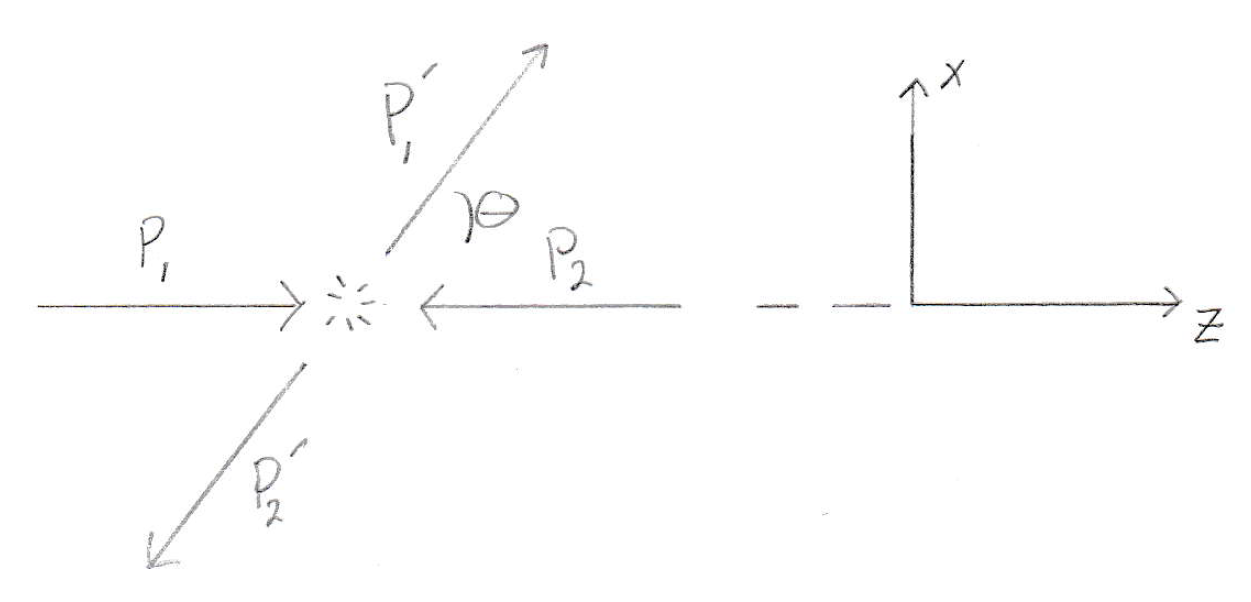
\includegraphics[width=0.8\textwidth]{figures/scat3}
	\caption{The kinematics of massive scattering.}
	\label{fig:shi}
\end{figure}
\begin{equation}
	p_1=\begin{bmatrix}
		E_1 \\ 0\\ 0 \\ p_{1z} \\
	\end{bmatrix} ,\quad
	p_2=\begin{bmatrix}
		E_2 \\ 0\\ 0\\ p_{2z}\\
	\end{bmatrix},\quad 
	p'_1=\begin{bmatrix}
		E'_1 \\ p'_{1x}\\ 0 \\ p'_{1z} \\
	\end{bmatrix} \quad \text{and}\quad
	p'_2=\begin{bmatrix}
		E'_2 \\ p'_{2x}\\ 0\\ p'_{2z}\\
	\end{bmatrix}.
\end{equation} 
In order to evaluate the three dimensional integrals in the phase space faction the delta function is split up as follows
\begin{equation}
	\delta^{(4)}(p_1+p_2-p'_1-p'_2)=\delta(E_1+E_2-E_1'-E'_2)\delta^{(3)}(\vec{p}_1+\vec{p}_2-\vec{p'}_1-\vec{p'}_2).
\end{equation} 
By using the three-dimensional delta-function the integral over $d^3p'_2$ becomes trivial and it is evaluated by setting $\vec{p'}_2=\vec{p}_1+\vec{p}_2-\vec{p'}_1=-\vec{p'}_1\Rightarrow E'_2=E'_2(p'_1)$. By using this
\begin{equation}
	\begin{split}
		\int d\Phi^{(2)}&=\int\frac{d^3p_1'}{(2\pi)^3}\frac{1}{2E_1 '}(2\pi)^4\delta(E_1+E_2-E_1'-E'_2)\int\frac{d^3p'_2}{(2\pi)^3}\frac{1}{2E'_2}\delta^{(3)}(\vec{p}_1+\vec{p}_2-\vec{p'}_1-\vec{p'}_2)\\
		&=\int\frac{d^3p_1'}{(2\pi)^3}\frac{(2\pi)\delta(E_1+E_2-E_1'-E'_2)}{4E'_1E_2'}.\\
	\end{split}
\end{equation} 
Next go to spherical coordinates such that $d^3p_1'\Rightarrow |\vec{p'}_1|^2d|\vec{p'}_1|d\Omega$. Hereby
\begin{equation}
	\begin{split}
		\int d\Phi^{(2)}&=\int\frac{d\Omega}{4(2\pi)^2}   \int\frac{|\vec{p'}_1|^2d|\vec{p'}_1|}{E'_1E'_2}\delta(E_1+E_2-E'-E_2').
	\end{split}
\end{equation} 
In order to evaluate the integral the delta function is rewritten by using that $\delta(f(x))=\frac{\delta(x-x_0)}{|\frac{df(x)}{dx}|}$, where $x_0$ is the zero\footnote{If there are more than one zero there should be a sum.} of $f(x)$. By using this identity
\begin{equation}
	\delta(E_1+E_2-E'_1-E_2')=\delta(|\vec{p'}_1|-p_0')\frac{1}{|\vec{p'}_1|\big(\frac{1}{E'_1}+\frac{1}{E'_2}\big)},
\end{equation} 
where is the value of $|\vec{p'}_1|$ that fulfills $E_1+E_2-E'_1(|\vec{p'}_1|)-E_2'(|\vec{p'}_1|)=0$. This defines the on-shell value of $|\vec{p'}_1|$. By using the delta function
\begin{equation}
	\begin{split}
		\int d\Phi^{(2)}&=\int\frac{d\Omega}{16\pi^2}   \frac{p_0'}{E'_1+E'_2}.
		\end{split}
	\label{eq2}
\end{equation} 
By using equation \eqref{eq2} and \eqref{obs} the differential cross section can, in the CM rest frame, be written as
\begin{equation}
	\frac{d\sigma}{d\Omega}=\frac{S}{4F}\frac{1}{16\pi^2}   \frac{p_0'}{E'_1+E'_2}\braket{|\mathcal{M}|^2}.
	\label{shiess}
\end{equation} 
For a $2\Rightarrow 2$ scattering in the CM rest frame the flux factor can be written as
\begin{equation}
	\begin{split}
		F&\equiv E_1E_2|\vec{v}_1-\vec{v}_2|\\
		&=\sqrt{(p_1\cdot p_2)^2-m_1^2m_2^2}\\
		&=\sqrt{E_1^2E_2^2+2E_1E_2|\vec{p}_1||\vec{p}_2|+|\vec{p}_1|^2|\vec{p}_2|^2-m_1^2m_2^2}\\
		&=|\vec{p}_1|\sqrt{\frac{(|\vec{p}_1|^2+m_1^2)(|\vec{p}_1|^2+m_2^2)}{|\vec{p}_1|^2}+2E_1E_2+|\vec{p}_1|^2-\frac{m_1^2m_2^2}{|\vec{p}_1|^2}}\\
		&=|\vec{p}_1|(E_1+E_2)\\
		&=|\vec{p}_1|(E'_1+E'_2),
	\end{split}
\end{equation} 
where both energy and momentum conservation for the CM rest frame has been used. By using the expression of the flux factor in the differential cross section
\begin{equation}
	\frac{d\sigma}{d\Omega}=\frac{S}{64\pi^2}   \frac{\braket{|\mathcal{M}|^2}}{(E'_1+E'_2)^2}\frac{|\vec{p'}_1|}{|\vec{p}_1|}.
	\label{diffcrossmass}
\end{equation} 
The total cross section is then found by integrating over the solid angle. To this end the invariant amplitude must however be known since it can depend on the solid angle.

\section{Massless scattering}
\index{Kinematics of massless scattering}
The phase space factor under consideration is given by equation \eqref{kin1}. Considering the scattering event from the reference frame in which the massive particle is initially at rest, the respective coordinates can, cf. figure \ref{fig:11}, be described as
\begin{figure}[H]
	\captionsetup{width=1\textwidth}
	\centering
	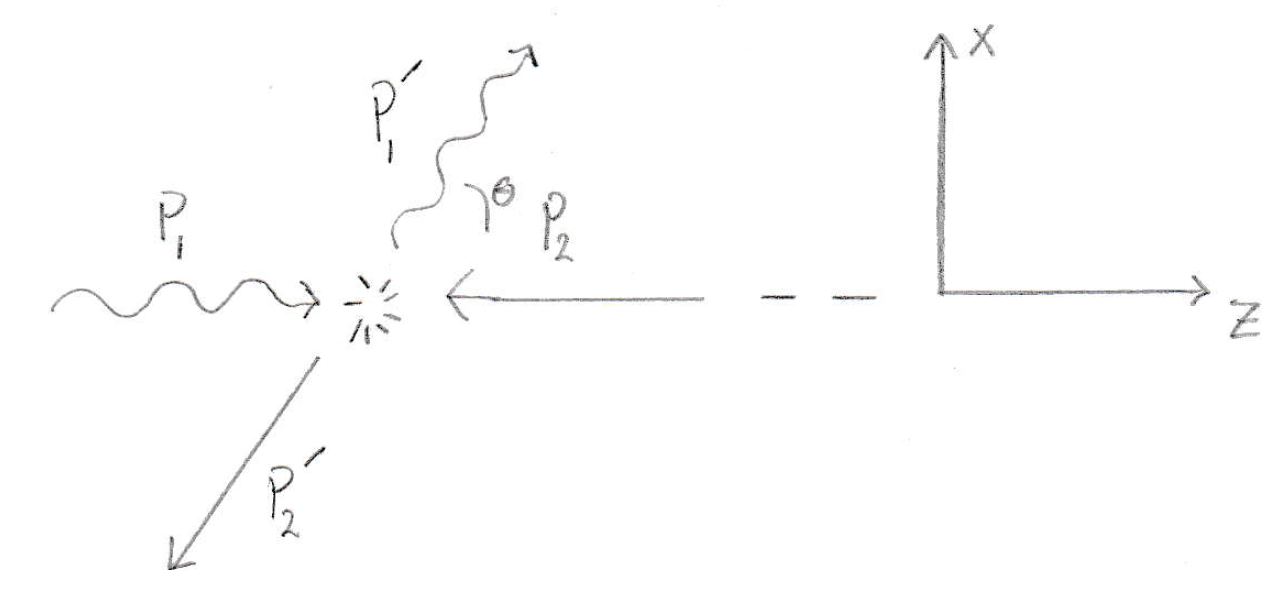
\includegraphics[width=0.8\textwidth]{figures/scat4}
	\caption{The kinematics of massless scattering.}
	\label{fig:11}
\end{figure}
\begin{equation}
	p_1=\begin{bmatrix}
		E_1 \\ 0\\ 0 \\ |\vec{p}_1| \\
	\end{bmatrix} ,\quad
	p_2=\begin{bmatrix}
		E_2 \\ -\vec{p}_1\\
	\end{bmatrix},\quad 
	p'_1=\begin{bmatrix}
		E'_1 \\ |\vec{p'}_1| \sin(\theta)\\ 0 \\ |\vec{p'}_1|\cos(\theta) \\
	\end{bmatrix} \quad \text{and}\quad
	p'_2=\begin{bmatrix}
		E'_2 \\ -\vec{p'}_1\\
	\end{bmatrix}, 
\end{equation} 
where $E_1=|\vec{p}_1|$ and $E'_1=|\vec{p'}_1|$.	As compared to the massive case, the massless case differs by the kinematics and the flux factor. The flux factor in the massless case is $F=\sqrt{(p_1\cdot p_2)^2-m_1^2m_2^2}=E_1 (E_2+E_1)=E_1E_{CM}=|\vec{p}_1|E_{CM}$ , where $E_{CM}\equiv E_1+E_2=E'_1+E'_2$. By using this in equation \eqref{shiess}
\begin{equation}
	\begin{split}
		\frac{d\sigma}{d\Omega}&=\frac{S}{4|\vec{p}_1| E_{CM}}\frac{1}{16\pi^2}   \frac{|\vec{p'}_1|}{E_{CM}}\braket{|\mathcal{M}|^2}\\
		&=\frac{S}{64\pi^2E_{CM}^2}   \frac{|\vec{p'}_1|}{|\vec{p}_1|}\braket{|\mathcal{M}|^2}.\\
	\end{split}
	\label{diffcrossmass1}
\end{equation} 

\section{$1\Rightarrow 2$ decay}
\index{Kinematics of $1\Rightarrow 2$ decay}
The phase space factor for $1\Rightarrow 2$ decay is given by
\begin{equation}
	\int d\Phi^{(2)}=\int\frac{d^3p'_1}{(2\pi)^3}\int\frac{d^3p'_2}{(2\pi)^3}\frac{(2\pi)^4\delta^{(4)}(p-p'_1-p_2')}{4E'_{1}E'_{2}}.
\end{equation} 
Considering the scattering event from the frame in which the initial particle is at rest, the respective coordinates can, cf. figure \ref{fig:21}, be described as
\begin{figure}[H]
	\captionsetup{width=1\textwidth}
	\centering
	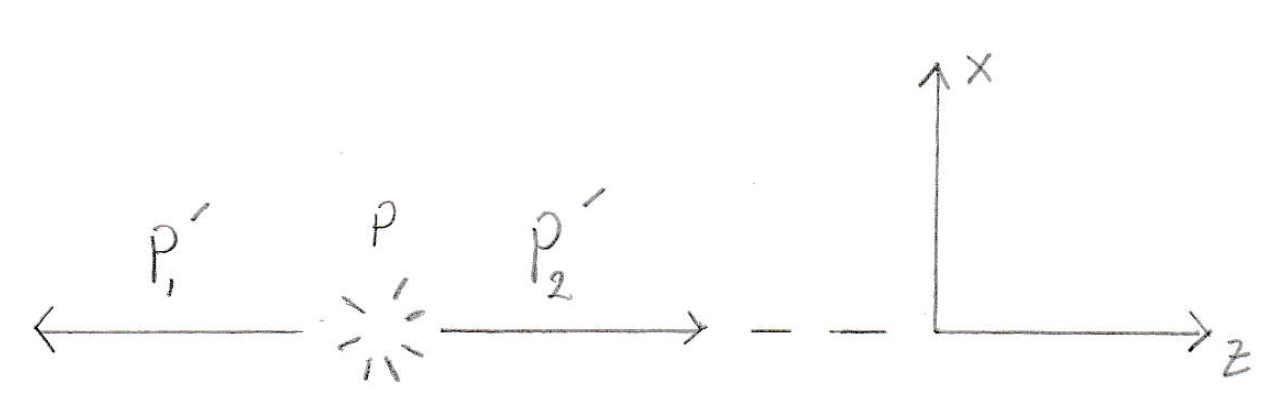
\includegraphics[width=0.8\textwidth]{figures/scat5}
	\caption{The kinematics of the decay.}
	\label{fig:21}
\end{figure}
\begin{equation}
	p=\begin{bmatrix}
		m \\ \vec{0}\\
	\end{bmatrix}, \quad 
	p_1'=\begin{bmatrix}
		E'_1 \\ \vec{p'}_1\\
	\end{bmatrix} \quad \text{and}\quad
	p_2'=\begin{bmatrix}
		E'_2 \\ \vec{p'}_2\\
	\end{bmatrix},
\end{equation}  
where from conservation of momentum, $k=q+p$
\begin{equation}
	\begin{bmatrix}
		m \\ \vec{0} \\
	\end{bmatrix}= \begin{bmatrix}
	E'_1+E'_2 \\ \vec{p'}_1+\vec{p'}_2\\
\end{bmatrix}.
\end{equation} 
Splitting the delta function
\begin{equation}
	\delta^{(4)}(p-p'_1-p'_2)=\delta(m-E'_1-E'_2)\delta^{(3)}(\vec{p'}_1+\vec{p'}_2).
\end{equation} 
From this the integration over $d^3p'_2$ can be eliminated, setting $\vec{p'}_1=-\vec{p'}_2$
\begin{equation}
	\begin{split}
		\int d\Phi^{(2)}&=\int\frac{d^3p'_1}{(2\pi)^3}\frac{(2\pi)\delta(m-E'_1-E'_2)}{4E'_{1}E'_{2}}\\
		&=\int \frac{d\Omega}{16\pi^2}\int \frac{|\vec{p'}_1|^2d|\vec{p'}_1|}{E'_{1}E'_{2}}\delta(m-E'_1-E'_2).\\
	\end{split}
	\label{int2}
\end{equation} 
To evaluate the integral the delta function must be rewritten in terms of the integration variable. Using that, because of the first integral, $E'_1=E_1'(|\vec{p'}_1|), E'_2=E_2'(|\vec{p'}_1|)$. By applying the same procedure as in the previous cases
\begin{equation}
	\delta(m-E'_1-E'_2)=\frac{E_1'}{|\vec{p'}_1|}\delta(|\vec{p'}_1|-p_0).
\end{equation} 
By using this in equation \ref{int2}
\begin{equation}
	\begin{split}
		\int d\Phi^{(2)}&=\int \frac{d\Omega}{16\pi^2}\int \frac{|\vec{p'}_1|d|\vec{p'}_1|}{E'_{2}}\delta(|\vec{p'}_1|-p_0)\\
		&=\int \frac{d\Omega}{16\pi^2}\frac{p_0}{E'_{2}}.\\
	\end{split}
	\label{int3}
\end{equation} 
By using equation \eqref{int3} alongside equation \eqref{obs}
\begin{equation}
	\frac{d\Gamma}{d\Omega}=\frac{S}{32\pi^2m}\frac{|\vec{p'}_1|}{E'_{2}}\braket{|\mathcal{M}|^2},
\end{equation} 
where it once more has been used that $p_0$ is the on-shell value of $|\vec{p'}_1|$ and so $p_0=|\vec{p'}_1|$ has been used in the end.

\section{The Invariant Matrix Element}
The invariant matrix element is defined in terms of the transition amplitude between two states. The amplitude is given by
\begin{equation}
	\mathcal{A}\equiv \braket{f|S|i},
	\label{S1}
\end{equation} 
where $S$ is the operator, called the scattering operator, evolving the initial state to the final state and
\begin{equation}
	\begin{split}
		&\ket{i}=\ket{\vec{p}_1}\otimes \ket{\vec{p}_2}\otimes \dots =\bigotimes_{i}\,\ket{\vec{p}_i}\\
		&\bra{f}=\dots \otimes \bra{\vec{p'}_2}\otimes \bra{\vec{p'}_1}=\bra{\vec{p'}_j}\bigotimes_j.
	\end{split}
\end{equation} 
For future reference I will use $p$ as initial momenta and $p'$ as final momenta. If $S=1$ there are no scattering between the particles and $\mathcal{A}$ is only non-vanishing if the initial and final state are equal. Motivated by this the $S$-operator is defined in terms of a non-interacting ($1$) and interacting ($T$) part cf.
\begin{equation}
	S\equiv 1+iT.
	\label{S2}
\end{equation} 
Using this definition in $\mathcal{A}$ leads to the definition of the invariant matrix element. $\mathcal{A}$ in terms of $T$ is given by
\begin{equation}
	\mathcal{A}=\braket{f|i}+\braket{f|iT|i}.
	\label{S3}
\end{equation} 
The $T$-part always carry a delta function securing momentum conservation at the vertexes. This is by convention factored from the last term alongside a factor of $(2\pi)^4$. Hereby
\begin{equation}
	\begin{split}
		\mathcal{A}&=\braket{f|i}+(2\pi)^4\delta^{(4)}(\Sigma p'-\Sigma p)\underbrace{\frac{\braket{f|iT|i}}{(2\pi)^4\delta^{(4)}(\Sigma p'-\Sigma p)}}_{\equiv i\mathcal{M}}\\
		&=\braket{f|i}+(2\pi)^4\delta^{(4)}(\Sigma p'-\Sigma p)i\mathcal{M}.
	\end{split}
	\label{S4}
\end{equation} 
So, the invariant matrix element is defined from the interactive part of a transition amplitude. The invariant matrix element is most often calculated from Feynman diagrams and Feynman rules.  However, it can also be done by a more rigorous procedure - the one used before Feynman diagrams; by relating $\mathcal{M}$ to the n-point functions of the theory. The relationship between the invariant matrix element and the n-point functions depend on the theory, and so in order to illustrate the relationship I have to pick a theory. To keep it simple I will consider an interactive scalar theory, eg. $\phi^4$-theory. The formula I am looking for, relation the invariant matrix element to the n-point functions of the theory, is called the LSZ reduction formula.

\subsection*{The LSZ Reduction Formula}
Consider the transition amplitude
\begin{equation}
	\mathcal{A}=\underbrace{\braket{f|S|i}}_{\text{Schroedinger scheme}}=\underbrace{\braket{f,t_f|S|i,t_i}}_{\text{Heisenberg scheme}}.
\end{equation} 
Since the goal is to relate the invariant matrix element to the n-point functions (which are on the form $\braket{\Omega|T\{\dots\}|\Omega}$), it is desired to somehow to "remove" the particles from the states and represent them by fields in between the states. Particles can be "pulled" from states by using that $\ket{\vec{p}}=\sqrt{2E_{\vec{p}}}a_{\vec{p}}^\dagger\ket{0}$. The ladder operators are then related to the fields, so intuitively the idea seems reasonable. For a \emph{free} theory the field can be expressed in terms of the mode expansion. This expression can be inverted to isolate the ladder operators to find
\begin{equation}
	\sqrt{2E_{\vec{p}}}\,a_{\vec{p}}=i\int d^3x e^{ip\cdot x}\overleftrightarrow{\partial}_0\phi_{free}, \quad \sqrt{2E_{\vec{p}}}\,a_{\vec{p}}^\dagger=-i\int d^3x e^{-ip\cdot x}\overleftrightarrow{\partial}_0\phi_{free},
\end{equation} 
where
\begin{equation}
	e^{ip\cdot x} \overleftrightarrow{\partial}_0\phi_{free}=e^{ip\cdot x}\partial_0\phi_{free}-\phi_{free}\partial_0e^{ip\cdot x}.
\end{equation} 
However, the fields under consideration are not free - they are interactive (recall the $\phi^4$-statement). However, interactive fields cannot be expanded in the mode expansion, so it is desired to relate the free fields to the interactive fields. To this end assume that infinitely far away in time, before and after the scattering, the fields are free. This assumption is reasonable for weakly interacting theories, but not in general - for example it is not reasonable for QCD. So, taking the theory under consideration to be weakly interacting
\begin{equation}
	\phi\xrightarrow{t\Rightarrow \pm\infty}\sqrt{Z}\phi_{out/in},
\end{equation} 
where $Z$ is the wave function renormalization factor and $\phi_{out/in}$ are free fields infinitely before and after in time. From these definitions
\begin{equation}
	\sqrt{2E_{\vec{p}}}\,a_{\vec{p}}^{in \dagger}=-iZ^{-\frac{1}{2}}\lim_{t\Rightarrow -\infty}\bigg(\int d^3x e^{-ip\cdot x}\overleftrightarrow{\partial}_0\phi\bigg),
\end{equation} 
where the field on the RHS is the field of the full theory, i.e. not the free field. From this definition one of the particles of the initial state can be "pulled" from the initial state via.
\begin{equation}
	\begin{split}
		\mathcal{A}&=\sqrt{2E_{\vec{p}_1}}\,\braket{\Sigma\vec{p'},t_f|a_{\vec{p}_1}^{in \dagger}|\Sigma\vec{p}-\vec{p}_1,t_i}\\
		&=-iZ^{-\frac{1}{2}}\lim_{t\Rightarrow -\infty}\bigg(\int d^3x e^{-ip_1\cdot x}\braket{\Sigma\vec{p'},t_f|\overleftrightarrow{\partial}_0\phi|\Sigma\vec{p}-\vec{p}_1,t_i}\bigg).\\
	\end{split}
\end{equation} 
It is desired to get rid of the limit in the above expression. In order to do this use the identity
\begin{equation}
	\bigg( \lim_{t\Rightarrow \infty} -\lim_{t\Rightarrow -\infty} \bigg)\int d^3x f(\vec{x},t)=\int_{-\infty}^{\infty}dt \frac{d}{dt}\bigg(\int d^3x f(\vec{x},t)\bigg).
\end{equation} 
To use this identity, the "subtracted limit" is needed. To get this, assume that there are no spectating particles - i.e. no particles that does not interact. If this is the case, then $\bra{\Sigma \vec{p'}}a_{\vec{p}}^{out\dagger}=0$. Since one can always add zero, the transition amplitude can be written as
\begin{equation}
	\mathcal{A}=\sqrt{2E_{\vec{p}_1}}\,\braket{\Sigma\vec{p'},t_f|(a_{\vec{p}_1}^{in \dagger}-a_{\vec{p_1}}^{out\dagger})|\Sigma\vec{p}-\vec{p}_1,t_i}.\\
\end{equation} 
By expressing $\sqrt{2E_{\vec{p}_1}}\,a_{\vec{p_1}}^{out\dagger}$ in terms of the field the identity can be used. Take $f(\vec{x},t)\rightleftarrows -iZ^{-\frac{1}{2}}e^{-ip_1\cdot x}\overleftrightarrow{\partial}_0\phi$. By using the identity, and swapping the time-derivative and integration over $d^3x$
\begin{equation}
	\sqrt{2E_{\vec{p}_1}}\,(a_{\vec{p}_1}^{in \dagger}-a_{\vec{p_1}}^{out\dagger})=iZ^{-\frac{1}{2}}\int d^4x \partial_0(e^{-ip_1\cdot x}\overleftrightarrow{\partial}_0\phi),
\end{equation} 
where the positive sign comes from the fact that $a_{\vec{p}_1}^{in \dagger}-a_{\vec{p_1}}^{out\dagger}\propto\lim_{t\Rightarrow -\infty} -\lim_{t\Rightarrow \infty}$. Applying the time derivatives and writing it out
 \begin{equation}
	\begin{split}
		\sqrt{2E_{\vec{p}_1}}\,(a_{\vec{p}_1}^{in \dagger}-a_{\vec{p_1}}^{out\dagger})&=iZ^{-\frac{1}{2}}\int d^4x \partial_0(e^{-ip_1\cdot x}\overleftrightarrow{\partial}_0\phi)\\
		&=iZ^{-\frac{1}{2}}\int d^4x \partial_0(e^{-ip_1\cdot x}\partial_0\phi+iE_{\vec{p}_1}e^{-ip_1\cdot x}\phi)\\
		&=iZ^{-\frac{1}{2}}\int d^4x (-iE_{\vec{p}_1}e^{-ip_1\cdot x}\phi+e^{-ip_1\cdot x}\partial_0^2\phi+E_{\vec{p}_1}^2e^{-ip_1\cdot x}\phi+iE_{\vec{p}_1}e^{-ip_1\cdot x}\phi) \\
		&=iZ^{-\frac{1}{2}}\int d^4x e^{-ip_1\cdot x}(\partial_0^2+E_{\vec{p}_1}^2)\phi \\
		&=iZ^{-\frac{1}{2}}\int d^4x e^{-ip_1\cdot x}(\partial_0^2+m_{\vec{p}_1}^2+(\vec{p}_1)^2)\phi \\
		&=iZ^{-\frac{1}{2}}\int d^4x (e^{-ip_1\cdot x}\partial_0^2\phi+\phi(m_{\vec{p}_1}^2-\nabla^2)e^{-ip_1\cdot x})\\
		&=iZ^{-\frac{1}{2}}\int d^4x (e^{-ip_1\cdot x}(\square_x+m_{\vec{p}_1}^2)\phi,\\
	\end{split}
\end{equation} 
where integration by parts has been used twice to shift $\nabla^2$ from the exponential to $\phi$. From using the above the transition amplitude is given by
\begin{equation}
	\mathcal{A}=iZ^{-\frac{1}{2}}\int d^4x e^{-ip_1\cdot x}(\square _x+m_{\vec{p}_1}^2)\braket{\Sigma\vec{p'},t_f|\phi(x)|\Sigma\vec{p}-\vec{p}_1,t_i}.
\end{equation} 
By continuing this way all particles from the initial and final states can be removed and represented by fields instead. Denoting the "position belonging to the final-state particles" by $y$ and the "position belonging to the initial-state particles" by $x$ the transition amplitude can therefore be written as
\begin{equation}
	\begin{split}
		\mathcal{A}&=\bigg(i\frac{1}{\sqrt{Z}}\bigg)^{n+m}\int\prod_{i=1}^m d^4x_i\int\prod_{j=1}^n d^4y_ie^{i(p'_j\cdot y_j-p_i\cdot x_i)}(\square _{x_i}+m_{\vec{p}_i}^2)(\square _{y_j}+m_{\vec{p'}_j}^2)\\
		&\quad\cdot\braket{\Omega|T\{\phi(x_1)\dots\phi(x_m)\phi(y_1)\dots \phi(y_n)\}|\Omega}.\\
	\end{split}
	\label{am}
\end{equation} 
However, since no spectating particles has been assumed, equation \eqref{am} only denotes the interactive part of the transition amplitude. Therefore
\begin{equation}
	\begin{split}
		\braket{f|iT|i}&=\bigg(i\frac{1}{\sqrt{Z}}\bigg)^{n+m}\int\prod_{i=1}^m d^4x_i\int\prod_{j=1}^n d^4y_ie^{i(p'_j\cdot y_j-p_i\cdot x_i)}(\square _{x_i}+m_{\vec{p}_i}^2)(\square _{y_j}+m_{\vec{p'}_j}^2)\\
		&\quad\cdot\braket{\Omega|T\{\phi(x_1)\dots\phi(x_m)\phi(y_1)\dots \phi(y_n)\}|\Omega}.\\
	\end{split}
	\label{am1}
\end{equation} 
Equation \eqref{am1} is a version of the so-called LSZ formula which relates the interactive part of the transition amplitude to the n-point functions of the interactive theory. Similar expressions can be obtained for fermion or boson fields by repeating a similar procedure. The result will be a similar expression with different fields, a possible minus sign (due to anti-commutation of fermion fields) and the Dirac operator instead of the KG operator. Note that $\phi(x)$ is not a free field, but a field of the entire field. This is the reason why $(\square +m^2)\phi\neq0$, i.e. the KG equation is only valid for free fields. 

\subsection*{Perturbation theory in QFT}
After having related the n-point functions for the interactive theory to the invariant matrix element it is time to determine the n-point functions themselves. Recall that an interactive theory is considered, so for example the two-point function is not the propagator. This is only the case for a free theory - i.e. a non-interactive theory. What is desired is to relate the n-point functions of the interactive theory to the n-point functions of the free theories, i.e. relate the interactive fields to the free fields and the interactive vacuum state to the free vacuum state. To this end use what is called the interaction scheme of QM. In this scheme both the states and operators are time-dependent cf.
\begin{equation}
	\ket{\psi_I(t)}\equiv e^{iH_0t}\ket{\psi_S(t)},\quad A_I(t)\equiv e^{iH_0t}A_Se^{-iH_0t},
\end{equation} 
where $I$ denotes the interaction scheme, $S$ denotes the Schroedinger scheme and $H_0$ is the free part of an interactive Hamiltonian. The interactive theory is characterized by a Lagrangian density on the form
\begin{equation}
	\mathcal{L}=\mathcal{L}_{0}+\mathcal{L}_{int},
	\label{lag}
\end{equation} 
where $\mathcal{L}_{0}=\mathcal{L}_{free}$. Equation \eqref{lag} is true for all theories, not only scalar field theories. The Lagrangian density corresponds to a Hamiltonian density on the form
\begin{equation}
	\mathcal{H}=\mathcal{H}_{0}+\mathcal{H}_{int}.
\end{equation} 
The solution to the EOM's for the interactive theory is in general very difficult (at best) to obtain. Since the theory is not free it is however clear that the field will not be given in terms of a simple mode expansions. However, the interactive field can bed related to the free field by using the interaction scheme. Since the free field in the mode expansion is represented in the Heisenberg scheme, and $A_H(t)=e^{iHt}A_Se^{-iHt}$, the interactive field can be related to the free field in the interactive scheme via.
\begin{equation}
	\phi(x)=U^\dagger(t,t_0)\phi_I(x)U(t,t_0),
\end{equation} 
where\footnote{Note that $[H_{0},H]\neq 0$ in general so the exponentials cannot be "collected".} $U(t,t_0)=e^{iH_0(t-t_0)}e^{-iH(t-t_0)}$ is the time-evolution operator and $\phi_I(x)$, the field in the interactive scheme, is a free field so it can be written in terms of the mode expansion,  i.e.
\begin{equation}
	\phi_I(x)=\int \frac{d^3 p}{(2\pi)^3}\frac{1}{\sqrt{2E_{\vec{p}}}}\bigg(a_{\vec{p}}\,e^{-ip\cdot x}+a_{\vec{p}}^*\,e^{ip\cdot x}\bigg)=\text{free field}.
\end{equation} 
The time-evolution operator, $U$, obeys the Schroedinger equation in the interaction picture. This can be seen by
\begin{equation}
	i\frac{\partial U(t,t_0)}{\partial t}=e^{iH_0(t-t_0)}(H-H_0)e^{-H(t-t_0)}=\underbrace{e^{iH_0(t-t_0)}H_{int}e^{-iH_0(t-t_0)}}_{\equiv H_I}U(t,t_0),
\end{equation} 
where $H_I=H_I(t)$ is the interaction Hamiltonian in the interaction picture. The Schroedinger equation can be solved to find
\begin{equation}
	U(t,t_0)=T\{e^{-i\int d^4x \mathcal{H}_I}\}\Rightarrow S\equiv T\{e^{-i\int_{-\infty}^{\infty} d^4x \mathcal{H}_I}\}.
	\label{S}
\end{equation} 
With the time-evolution operator in the interaction scheme expressed, and the interactive field expressed in terms of free fields and the time-evolution operator in the interaction scheme, I have related the interactive fields to the free fields - as I wanted. Next up is the relationship between the vacuum state of the interactive theory and the vacuum state of the free theory. In order to relate the two I consider
\begin{equation}
	\begin{split}
		e^{-iHt}\ket{0}&=\sum_n
		e^{-iHt}\ket{n}\braket{n|0}\\
		&=e^{-iE_0t}\ket{\Omega}\braket{\Omega|0}+\sum_{n\neq \Omega}e^{-iHt}\ket{n}\braket{n|0},\\
	\end{split}
\end{equation} 
where $\ket{n}$ are eigenstates of the full theory and $E_0<e_{n\neq 0}$. To get "rid" of the second term, employ a mathematical trick; let $t\Rightarrow T\Rightarrow \infty (1-i\varepsilon)$ - where $T$ just denotes complex time. Because $E_0<e_{n\neq 0}$ the $E_0$ term will die out last. Therefore, in the limit of $T\Rightarrow \infty (1-i\varepsilon)$
\begin{equation}
	\ket{\Omega}=\lim\limits_{T\Rightarrow \infty (1-i\varepsilon)}\bigg(\frac{e^{iHT}\ket{0}}{e^{-iE_0T}\braket{\Omega|0}}\bigg).
\end{equation} 
Since $T$ is taken in the limit of going to infinity, a small shift, $T\Rightarrow T+t_0$ makes no difference. Hereby
\begin{equation}
	\ket{\Omega}=\lim\limits_{T\Rightarrow \infty (1-i\varepsilon)}\bigg(\frac{e^{iH(T+t_0)}\ket{0}}{e^{-iE_0(T+t_0)}\braket{\Omega|0}}\bigg).
\end{equation} 
Use now that, since $H_0\ket{0}=0$
\begin{equation}
	e^{iH_0(T+t_0)}\ket{0}=(1-iH_0(T+t_0))\ket{0}=\ket{0}.
\end{equation} 
Hence, the vacuum state in the interactive theory can be written as
\begin{equation}
	\begin{split}
		\ket{\Omega}&=\lim\limits_{T\Rightarrow \infty (1-i\varepsilon)}\bigg(\frac{e^{iH(T+t_0)}e^{iH_0(T+t_0)}\ket{0}}{e^{-iE_0(T+t_0)}\braket{\Omega|0}}\bigg)\\
		&=\lim\limits_{T\Rightarrow \infty (1-i\varepsilon)}\bigg(\frac{U(t_0,T)\ket{0}}{e^{-iE_0(T+t_0)}\braket{\Omega|0}}\bigg).\\
	\end{split}
	\label{vacs}
\end{equation} 
By using equation \eqref{vacs} and the expression for $\phi$ in terms of $\phi_I$
\begin{equation}
	\braket{\Omega|T\{\phi(x_1)\dots \phi(x_N)\}|\Omega}=\lim\limits_{T\Rightarrow \infty (1-i\varepsilon)}\bigg(\frac{\braket{0|U^\dagger(t_0,T)[U(t_0,t)\phi_I(x_1)U(t,t_0)]\dots U(t_0,-T)|0}}{e^{-iE_0(2T)}|\braket{\Omega|0}|^2}\bigg).
\end{equation} 
To get rid of the denominator, I divide by
\begin{equation}
	1=\braket{\Omega|\Omega}=\frac{\braket{0|U(T,t_0)U(t_0,-T)|0}}{e^{-iE_0(2T)}|\braket{\Omega|0}|^2}.
\end{equation} 
Next collect the fields in the nominator under a time-ordering. By doing so the time-evolution operators can be collected to the exponential. Hereby the n-point function can be written as
\begin{equation}
	\braket{\Omega|T\{\phi(x_1)\dots \phi(x_N)\}|\Omega}=\lim\limits_{T\Rightarrow \infty (1-i\varepsilon)}\bigg(\frac{\braket{0|T\{\phi_I(x_1)\dots\phi_I(x_N)e^{-i\int d^4x \mathcal{H}_I}\}|0}}{\braket{0|T\{e^{-i\int d^4x \mathcal{H}_I}\}|0}}\bigg).
	\label{pert}
\end{equation} 
The last step is then to expand the exponential in a Taylor series and use $\mathcal{H}_I$ from th interactive theory. $\mathcal{H}_I$ can be found from
\begin{equation}
	\mathcal{H}_I=e^{iH_0(t-t_0)}\mathcal{H}_{int}e^{-iH_0(t-t_0)}=\mathcal{H}_{int}(\phi_I).
\end{equation} 
Hence, $\mathcal{H}_I$ is the interactive part of the Hamiltonian density with $\phi\Rightarrow \phi_I=\text{free field}$. Collecting the results of equation \eqref{S4}, \eqref{am1} and \eqref{pert}
\begin{equation}
	\begin{split}
		i\mathcal{M}&=\frac{\braket{f|iT|i}}{(2\pi)^4\delta^{(4)}(\Sigma p'-\Sigma p)}\\
		&=\frac{\big(i\frac{1}{\sqrt{Z}}\big)^{n+m}}{(2\pi)^4\delta^{(4)}(\Sigma p'-\Sigma p)}\int\prod_{i=1}^m d^4x_i\int\prod_{j=1}^n d^4y_ie^{i(p'_j\cdot y_j-p_i\cdot x_i)}(\square _{x_i}+m_{\vec{p}_i}^2)(\square _{y_j}+m_{\vec{p'}_j}^2)\\
		&\qquad \cdot\braket{\Omega|T\{\phi(x_1)\dots\phi(x_m)\phi(y_1)\dots \phi(y_n)\}|\Omega}\\
		&=\frac{\big(i\frac{1}{\sqrt{Z}}\big)^{n+m}}{(2\pi)^4\delta^{(4)}(\Sigma p'-\Sigma p)}\int\prod_{i=1}^m d^4x_i\int\prod_{j=1}^n d^4y_ie^{i(p'_j\cdot y_j-p_i\cdot x_i)}(\square _{x_i}+m_{\vec{p}_i}^2)(\square _{y_j}+m_{\vec{p'}_j}^2)\\
		&\qquad\cdot \lim\limits_{T\Rightarrow \infty (1-i\varepsilon)}\bigg(\frac{\braket{0|T\{\phi_I(x_1)\dots\phi_I(y_n)e^{-i\int d^4x \mathcal{H}_I}\}|0}}{\braket{0|T\{e^{-i\int d^4x \mathcal{H}_I}\}|0}}\bigg). 
	\end{split}
	\label{qw}
\end{equation} 
Equation \eqref{qw} is valid for a generic scalar theory.

\begin{example}
	\emph{Consider a scattering amplitude for a process with two initial particles, with momenta $\vec{p}_1$ and $\vec{p}_2$, into two final particles, with momenta $\vec{p'}_1$ and $\vec{p'}_2$, in $\phi^4$-theory. Take the interactive part of the Hamiltonian density to be on the form}
	\begin{equation}
		\mathcal{H}_I=\frac{\lambda}{4!}\phi^4,
	\end{equation} 
	\emph{where $\phi=\phi_I$ in this example. The coupling, $\lambda$, defines the strength of the interaction. }
	\begin{enumerate}
		\item \emph{Draw the Feynman diagrams in position space. Compute the amplitude in the case in which there is no interactions, i.e. for $\lambda=0$, and motivate why there is no contribution as expected.}
		
		I begin by writing writing explicitly the LSZ formula, with the KG operators taken to the LHS and represented in momentum space, for $\phi^4$-theory
		\begin{equation}
			\begin{split}
				&\bigg(\prod_{i=1}^{2}\frac{i\sqrt{Z}}{p'_i-m^2}\bigg)\bigg(\prod_{j=1}^{2}\frac{i\sqrt{Z}}{p_j-m^2}\bigg)\braket{\vec{p'}_1\vec{p'}_2|iT|\vec{p}_1\vec{p}_2}=\int d^4x_1\int d^4x_2\int d^4x_3\int d^4x_4\\
				&\cdot e^{i(p'_1\cdot x_1+p'_2\cdot x_2-p_1\cdot x_3-p_2\cdot x_4)}\frac{\braket{0|T\{\phi(x_1)\phi(x_2)\phi(x_3)\phi(x_4)e^{-i\frac{\lambda}{4!}\int d^4x\phi^4}\}|0}}{\braket{0|T\{e^{-i\frac{\lambda}{4!}\int d^4x \phi^4}\}|0}}.
			\end{split}
		\end{equation}  
		I take the lowest non-trivial order in perturbation theory - Ie. I will work to $\mathcal{O}(\lambda)$. In this theory
		\begin{equation}
			Z=1+\mathcal{O}(\lambda^2).
		\end{equation} 
		Therefore, I take $Z=1$. I also expand the exponential cf.
		\begin{equation}
			e^{-i\frac{\lambda}{4!}\int d^4x \phi^4}=1-i\frac{\lambda}{4!}\int d^4x\phi^4+\mathcal{O}(\lambda^2).
		\end{equation} 
		To $\mathcal{O}(\lambda^0)$, with $Z=1$, I find from the LSZ formula
		\begin{equation}
			\begin{split}
				&\frac{i}{p'_1-m^2}\frac{i}{p'_2-m^2}\frac{i}{p_1-m^2}\frac{i}{p_2-m^2}\braket{\vec{p'}_1\vec{p'}_2|iT|\vec{p}_1\vec{p}_2}=\int d^4x_1\int d^4x_2\int d^4x_3\int d^4x_4\\
				&\cdot e^{i(p'_1\cdot x_1+p'_2\cdot x_2-p_1\cdot x_3-p_2\cdot x_4)}\braket{0|T\{\phi(x_1)\phi(x_2)\phi(x_3)\phi(x_4)\}|0}.
			\end{split}
		\end{equation}  
		The VEV is computed by using Wicks theorem\index{Wicks theorem}. Wicks theorem states that a time-ordered series of field-operators is related to the normal-ordered series of field-operators, via.
		\begin{equation}
			T\{\phi_1\phi_2\dots\phi_n\}=N\{\phi_1\phi_2\dots\phi_n+\text{All contractions}\}.
		\end{equation} 
		Wicks theorem is extremely useful when considering a VEV, because the normal ordered product of free field operators vanish\footnote{Because the normal-ordering operator acts to put the annihilation operators to eh right, they will act on the vacuum and make the term vanish.}. The only terms that does not vanish are the ones which are fully contracted. For the VEV under consideration
		\begin{equation}
			\begin{split}
				VEV&=\braket{0|T\{\phi_1\phi_2\phi_3\phi_4\}|0}\\
				&
				\contraction{,,,,,,,,,,,,,,,,,,,,}{\phi_1}{.}{\phi_2}
				\contraction{,,,,,,,.,,,,,,,,,,,,,,,,,,,,,,,,,}{\phi_1}{,,}{\phi_2}
				\contraction{,,,,,,,,,,,,,,,,,,,,,,.,,,,,,,,,,,,,,,,,,,,,,}{\phi_1}{,,,,}{\phi_2}
				\contraction{,,,,,,,,,,,,,,,,,,,,,,,,.,,,,,,,,,,,,,,,,,,,,,,,,,,,,,,,,,,}{\phi_1}{.}{\phi_2}
				=\braket{0|N\{\phi_1\phi_2\phi_3\phi_4+\phi_1\phi_2\phi_3\phi_4+\phi_1\phi_2\phi_3\phi_4+\phi_1\phi_2\phi_3\phi_4+\phi_1\phi_2\phi_3\phi_4}\\
					&{
					\contraction{,,,,,}{\phi_1}{,,}{\phi_2}
					\contraction{,,,,,,,,,,,.,.,,,,,,}{\phi_1}{.}{\phi_2}
					\contraction{,,,,,,,,,,,,,,,,,,,,,,,,,,}{\phi_1}{.}{\phi_2}
					\contraction{,,,,,,,,,,,,,,,,,,,,,,,,,,,,,,,}{\phi_1}{.}{\phi_2}
					\contraction[2ex]{,,,,,,,,,,,,,,,,,,,,,,,,,,,,,,,,,,,,,,}{\phi_1}{,,,}{\phi_2}
					\contraction{,,,,,,.,,,,,,,,,,,,,,,,,,,,,,,,,,,,,,,,,,}{\phi_1}{.,,}{\phi_2}
					\contraction[2ex]{,,,,,,,,,,,,,,,,,,,,,,,,,,,,,,,,,,,,,,,,,,,,,,,,,,}{\phi_1}{,,,,.,}{\phi_2}
					\contraction{,,,,,,.,,,,,,,,,,,,,,,,,,,,,,,,,,,,,,,,,,,,,,,,,,,,,,}{\phi_1}{.}{\phi_2}
					+\phi_1\phi_2\phi_3\phi_4+\phi_1\phi_2\phi_3\phi_4+\phi_1\phi_2\phi_3\phi_4+\phi_1\phi_2\phi_3\phi_4+\phi_1\phi_2\phi_3\phi_4\}|0}.\\
			\end{split}
		\end{equation} 
		Now use that the contractions are complex numbers and as such they can be moved outside the Normal-ordering operator and bracket. Hence, what remains, besides the contraction, for fully contracted terms is $\braket{0|N\{1\}|0}=1$. Hereby
		\begin{equation}
			\contraction{,,,,,,,,,,,,,.,,,,,,.,}{\phi_1}{.}{\phi_2}
			\contraction{,,,,,,,,,,,,,,.,,,,,,,,,,,}{\phi_1}{.}{\phi_2}
			\contraction[2ex]{,,,,,,,,,,,,,,,,,,,,,,,,,,,,,,,,,}{\phi_1}{,,,}{\phi_2}
			\contraction{,,,,,,.,,,,,,,,..,,,,,,,,,,,,,,,,,,,,}{\phi_1}{..,}{\phi_2}
			\contraction[2ex]{,,,,,,,,,,,,,,.,,,,,,,,,,,,,,,,,,,,,,,,,,,,,,,}{\phi_1}{,,,,.}{\phi_2}
			\contraction{,,,,,,.,,,,,,,,,,,,,,,,,,,,,,,,,,,,,,,,,,,,,,,,,}{\phi_1}{.}{\phi_2}
			\braket{0|T\{\phi_1\phi_2\phi_3\phi_4\}|0}=\phi_1\phi_2\phi_3\phi_4+\phi_1\phi_2\phi_3\phi_4+\phi_1\phi_2\phi_3\phi_4.
		\end{equation} 
		Defining now
		\begin{equation}
			\contraction{}{\phi_1}{,,}{\phi_2}
			\phi(x_i)\phi(x_j)\equiv D(x_i-x_j)=D_{ij}.
		\end{equation} 
		The VEV becomes
		\begin{equation}
			\braket{0|T\{\phi_1\phi_2\phi_3\phi_4\}|0}=D_{12}D_{34}+D_{13}D_{24}+D_{14}D_{23}.
		\end{equation} 
		The VEV can be represented by Feynman diagrams
		\begin{figure}[H]
			\captionsetup{width=1\textwidth}
			\centering
			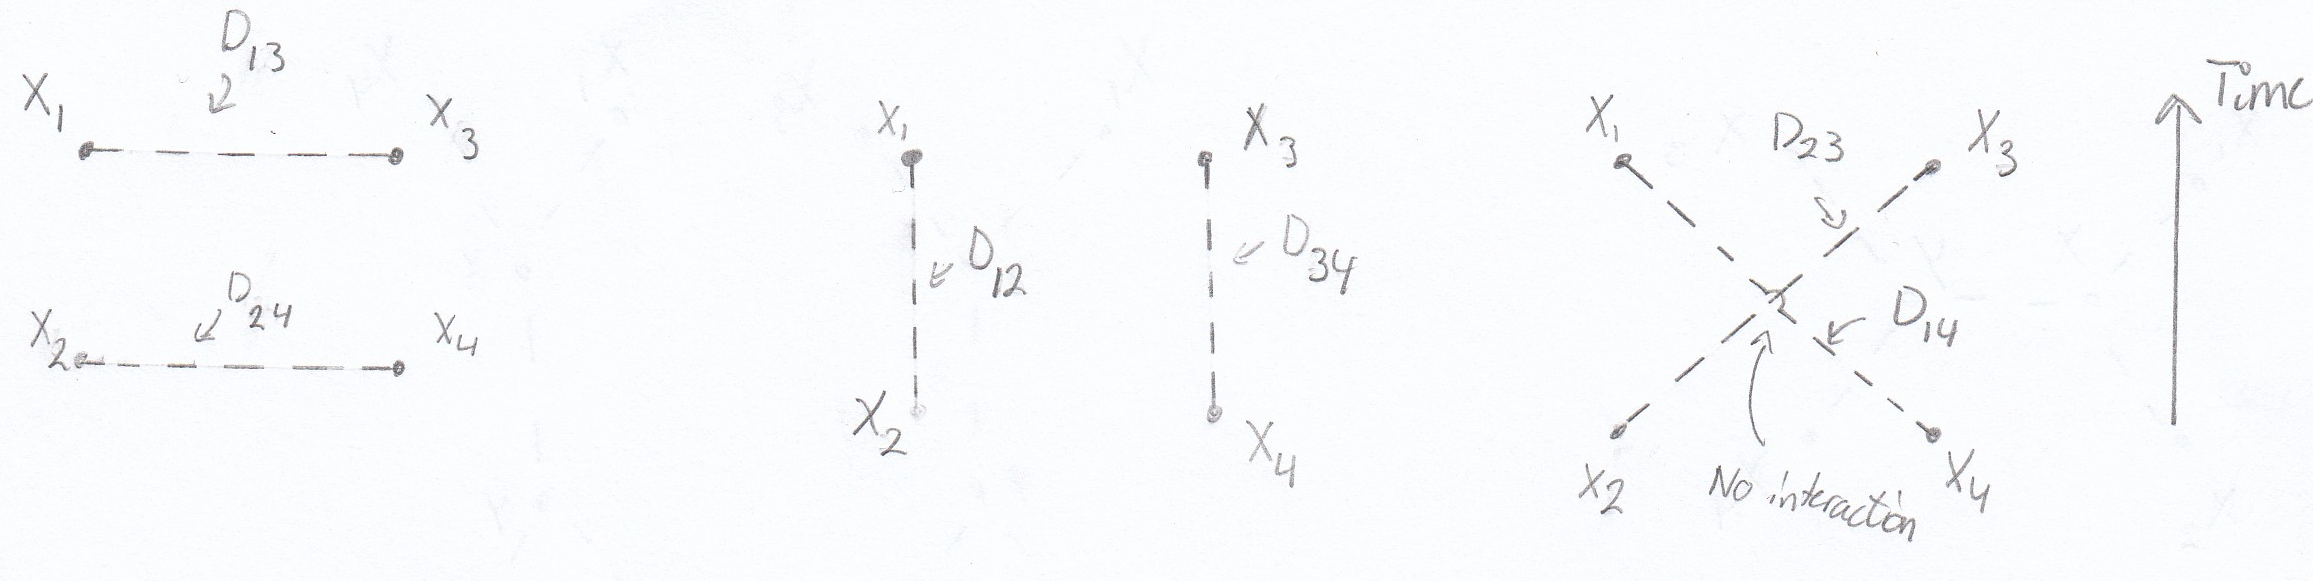
\includegraphics[width=0.9\textwidth]{figures/scal}
		\end{figure} 
		The diagrams show two particles traveling between two separate space-time-points without interacting. By using the expression for the VEV in the LSZ reduction formula to $\mathcal{O}(\lambda^0)$, with $z=1$, reveals
		\begin{equation}
			\begin{split}
				&\frac{i}{p'_1-m^2}\frac{i}{p'_2-m^2}\frac{i}{p_1-m^2}\frac{i}{p_2-m^2}\braket{\vec{p'}_1\vec{p'}_2|iT|\vec{p}_1\vec{p}_2}=\int d^4x_1\int d^4x_2\int d^4x_3\int d^4x_4\\
				&\cdot e^{i(p'_1\cdot x_1+p'_2\cdot x_2-p_1\cdot x_3-p_2\cdot x_4)}(D_{12}D_{34}+D_{13}D_{24}+D_{14}D_{23}).
			\end{split}
		\end{equation} 
		There are three integrals, of the propagators, to be evaluated. The first
		\begin{equation}
			I_1\equiv \int d^4x_1\int d^4x_2\int d^4x_3\int d^4x_4 e^{i(p'_1\cdot x_1+p'_2\cdot x_2-p_1\cdot x_3-p_2\cdot x_4)}D(x_1-x_2)D(x_3-x_4).
		\end{equation} 
		To evaluate $I_1$ I take $x'=x_1-x_2, x''=\frac{1}{2}(x_1+x_2),x'''=x_3-x_4,x''''=\frac{1}{2}(x_3+x_4)$. Hereby
		\begin{equation}
			\begin{split}
				I_1&\equiv \bigg(\underbrace{\int d^4x' \int d^4x''e^{i(p'_1+p'_2)x''}e^{\frac{i}{2}(p'_1-p'_2)x'}D(x')}_{\equiv I_4}\bigg)\\
				&\qquad\cdot\bigg(\underbrace{\int d^4x''' \int d^4x''''e^{-i(p_1+p_2)x''''}e^{-\frac{i}{2}(p_1-p_2)x'''}D(x''')}_{\equiv I_5}\bigg).\\
			\end{split}	
		\end{equation}  
		Now
		\begin{equation}
			\begin{split}
				I_4&=\int d^4x' \int d^4x''e^{i(p'_1+p'_2)x''}e^{\frac{i}{2}(p'_1-p'_2)x'}D(x')\\
				&=(2\pi)^4\delta^{(4)}(p'_1+p'_2)\int\frac{d^4p'}{(2\pi)^4}\frac{i}{p'^2-m^2}\underbrace{\int d^4x'e^{-i(p'-\frac{p'_1}{2}+\frac{p'_2}{2})\cdot x'}}_{=(2\pi)^4\delta^{(4)}(p'-\frac{p'_1}{2}+\frac{p'_2}{2})},
			\end{split}
		\end{equation} 
		where the propagator has been expressed in the momentum representation\footnote{Using $D(x_1-x_2)=\int\frac{d^4p'}{(2\pi)^4}\frac{i}{p'^2-m^2}e^{-ip'\cdot(x_1-x_2)}$.}. Now, use $\delta^{(4)}(p'_1+p'_2)\Rightarrow p_1'=-p_2'$ in $\delta^{(4)}(p'-\frac{p'_1}{2}+\frac{p'_2}{2})$. Hereby $\delta^{(4)}(p'-p_1')$. Hence, the integral can be killed off to reveal
		\begin{equation}
			I_4=\frac{(2\pi)^4}{p_1'^2-m^2}.
		\end{equation} 
		Likewise
		\begin{equation}
			\begin{split}
				I_5&=(2\pi)^4\delta^{(4)}(p_1+p_2)\int\frac{d^4p}{(2\pi)^4}\frac{i}{p^2-m^2}\underbrace{\int d^4x''''e^{-i(p+\frac{p_1}{2}-\frac{p_2}{2})\cdot x''''}}_{=(2\pi)^4\delta^{(4)}(p+\frac{p_1}{2}-\frac{p_2}{2})}.
			\end{split}
		\end{equation} 
		Repeating the procedure results in $k_1=-k_2\Rightarrow \delta^{(4)}(p+\frac{p_1}{2}-\frac{p_2}{2})=\delta^{(4)}(p+p_1)$. Hence, the integral will let $p=-p_1$. However, only $p^2$ is present in the integral, so $(-p_1)^2=p_1^2$. Hence
		\begin{equation}
			I_5=\frac{(2\pi)^4}{p_1^2-m^2}.
		\end{equation} 
		Putting $I_4$ and $I_5$ together
		\begin{equation}
			I_1=(2\pi)^8\frac{i}{p_1'^2-m^2}\frac{i}{p_1^2-m^2}.
		\end{equation}  
		For $I_2$ I define $x'=x_1-x_3, x''\frac{1}{2}(x_1+x_3), x'''=x_2-x_4, x''''=\frac{1}{2}(x_2+x_4)$. From these definitions $i(p'_1\cdot x_1+p'_2\cdot x_2-p_1\cdot x_3-p_2\cdot x_4)=\frac{i}{2}(p'_1+p_1)\cdot x'+i(p'_1-p_1)\cdot x''+\frac{i}{2}(p'_2+p_2)\cdot x'''+i(p'_2-p_2)\cdot x''''$. This enables me to write the integral as
		\begin{equation}
			\begin{split}
				I_2&\equiv \int d^4x_1\int d^4x_2\int d^4x_3\int d^4x_4 e^{i(p'_1\cdot x_1+p'_2\cdot x_2-p_1\cdot x_3-p_2\cdot x_4)}D(x_1-x_3)D(x_2-x_4)\\
				&=\bigg(\underbrace{\int d^4x' \int d^4x''e^{i(p'_1-p_1)x''}e^{\frac{i}{2}(p'_1+p_1)x'}D(x')}_{\equiv I_4'}\bigg)\\
				&\qquad\cdot\bigg(\underbrace{\int d^4x''' \int d^4x''''e^{i(p'_2-p_2)x''''}e^{\frac{i}{2}(p'_2+p_2)x'''}D(x''')}_{\equiv I_5'}\bigg).\\
			\end{split}
		\end{equation} 
		Now
		\begin{equation}
			\begin{split}
				I_4'&=\underbrace{\int d^4x''e^{i(p'_1-p_1)x''}}_{=(2\pi)^4\delta^{(4)}(p'_1-p_1)}\int d^4x'e^{\frac{i}{2}(p'_1+p_1)x'}D(x')\\
				&=(2\pi)^4\delta^{(4)}(p'_1-p_1)\int\frac{d^4p'}{(2\pi)^4}\frac{i}{p'^2-m^2}\underbrace{\int d^4x'e^{-i(p'-\frac{p'_1}{2}-\frac{p_1}{2})\cdot x'}}_{(2\pi)^4\delta^{(4)}(p'-\frac{p'_1}{2}-\frac{p_1}{2})}.
			\end{split}
		\end{equation} 
		Let again $\delta^{(4)}(p'_1-p_1)\Rightarrow p'_1=p_1$ and $\delta^{(4)}(p'-\frac{p'_1}{2}-\frac{p_1}{2})=\delta^{(4)}(p'-p'_1)$. So
		\begin{equation}
			I_4'=(2\pi)^4\frac{i}{p_1^{'2}-m^2}.
		\end{equation} 
		Likewise
		\begin{equation}
			I_5'=(2\pi)^4\frac{i}{p_2^{'2}-m^2}.
		\end{equation} 
		Hence
		\begin{equation}
			I_2=(2\pi)^8\frac{i}{p_1^{'2}-m^2}\frac{i}{p_2^{'2}-m^2}.
		\end{equation} 
		$I_3$ can be found in the same way. The result is that $I_3=I_2$. Hence, the LSZ formula
		\begin{equation}
			\begin{split}
				I_1+I_2+I_3&=\frac{i}{p'_1-m^2}\frac{i}{p'_2-m^2}\frac{i}{p_1-m^2}\frac{i}{p_2-m^2}\braket{\vec{p'}_1\vec{p'}_2|iT|\vec{p}_1\vec{p}_2}\\
				&=(2\pi)^8\frac{i}{p_1'^2-m^2}\frac{i}{p_1^2-m^2}+(2\pi)^8\frac{i}{p_1^{'2}-m^2}\frac{i}{p_2^{'2}-m^2}\\
				&\quad+(2\pi)^8\frac{i}{p_1^{'2}-m^2}\frac{i}{p_2^{'2}-m^2}.\\
			\end{split}
		\end{equation}  
		From the above I can isolate $\braket{\vec{p'}_1\vec{p'}_2|iT|\vec{p}_1\vec{p}_2}$. The result is that
		\begin{equation}
			\braket{\vec{p'}_1\vec{p'}_2|iT|\vec{p}_1\vec{p}_2}=-(2\pi)^8(p_2^{'2}-m^2)(p_2^2-m^2)-2(2\pi)^8(p_1^2-m^2)(p_2^2-m^2).
		\end{equation} 
		Now I go on mass shell, i.e. I enforce $p_i^{'2}=m^2$ and $p_i^2=m^2$, and so it is clear that $\braket{\vec{p'}_1\vec{p'}_2|iT|\vec{p}_1\vec{p}_2}=0$. This will be the case whenever the poles on both sides do not match/cancel each other out! I could have guessed this result since $\braket{\dots|iT|\dots}$ describes the interaction part of the S-matrix and to zeroth order the particles do no interact - As illustrated by the Feynman diagrams in position space. In terms of Feynman diagrams; all disconnected diagrams will result in zero contribution.  
		
		\item\emph{Compute the amplitude to $\mathcal{O}(\lambda)$.}
		
		The first non-vanishing contribution to $\braket{\vec{p'}_1\vec{p'}_2|iT|\vec{p}_1\vec{p}_2}$ comes from $\mathcal{O}(\lambda)$. A fast way to see this is the following; the first non-vanishing order is given as the first order above $\mathcal{O}(\lambda^0)$ in which the number of fields from $\mathcal{H}_I$ and the scattering process is even! The reason for this is Wicks theorem. If there is an uneven number of fields they cannot all be contracted on the same time, and so the time-ordered series vanish. At $\mathcal{O}(\lambda)$, and $Z=1$, the LSZ formula is given by
		\begin{equation}
			\begin{split}
				&\bigg(\prod_{i=1}^{2}\frac{i\sqrt{Z}}{p'_i-m^2}\bigg)\bigg(\prod_{j=1}^{2}\frac{i\sqrt{Z}}{p_j-m^2}\bigg)\braket{\vec{p'}_1\vec{p'}_2|iT|\vec{p}_1\vec{p}_2}=\int d^4x_1\int d^4x_2\int d^4x_3\int d^4x_4\\
				&\cdot e^{i(p'_1\cdot x_1+p'_2\cdot x_2-p_1\cdot x_3-p_2\cdot x_4)}\bigg(-\frac{i\lambda}{4!}\bigg)\int d^4x	\frac{\braket{0|T\{\phi(x_1)\phi(x_2)\phi(x_3)\phi(x_4)\phi^4(x)\}|0}}{\braket{0|T\{1-i\frac{\lambda}{4!}\int d^4x \phi^4\}|0}}.
			\end{split}
		\end{equation} 
		To evaluate the VEV I once again use Wicks theorem. The number of contractions fill a full page\footnote{See notes from 8. semester.}, so I will not do it here. Instead I will jump to the result
		\begin{equation}
			\braket{0|T\{\phi(x_1)\phi(x_2)\phi(x_3)\phi(x_4)\phi^2(x)\}|0}=4!D(x_1-x)D(x_2-x)D(x_3-x)D(x_4-x).
		\end{equation} 
		The Feynman diagram in position space is given by
		\begin{figure}[H]
			\captionsetup{width=1\textwidth}
			\centering
			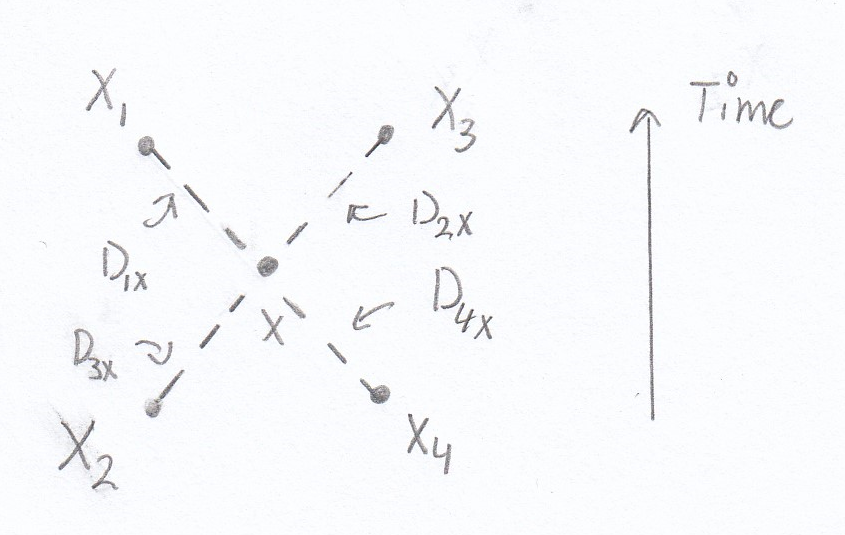
\includegraphics[width=0.5\textwidth]{figures/scal1}
		\end{figure}
		The factor of $4!$ cancels the factor of $\frac{1}{4!}$ from the Hamiltonian. Hereby, the I can write the LSZ reduction formula
		\begin{equation}
			\begin{split}
				&\frac{i}{p'_1-m^2}\frac{i}{p'_2-m^2}\frac{i}{p_1-m^2}\frac{i}{p_2-m^2}\braket{\vec{p'}_1\vec{p'}_2|iT|\vec{p}_1\vec{p}_2}=\int d^4x_1\int d^4x_2\int d^4x_3\int d^4x_4\\
				&\cdot e^{i(p'_1\cdot x_1+p'_2\cdot x_2-p_1\cdot x_3-p_2\cdot x_4)}(-i\lambda)\int d^4x\braket{0|T\{\phi(x_1)\phi(x_2)\phi(x_3)\phi(x_4)\phi^4(x)\}|0}\\
				&\cdot\frac{1}{\braket{0|T\{1-i\frac{\lambda}{4!}\int d^4x \phi^4\}|0}}.
			\end{split}
		\end{equation} 
		I consider
		\begin{equation}
			\begin{split}
				I&=\int d^4x_1\int d^4x_2\int d^4x_3\int d^4x_4e^{i(p'_1\cdot x_1+p'_2\cdot x_2-p_1\cdot x_3-p_2\cdot x_4)}\\
				&\qquad\cdot(-i\lambda)\int d^4x\braket{0|T\{\phi(x_1)\phi(x_2)\phi(x_3)\phi(x_4)\phi^4(x)\}|0}.
			\end{split}
		\end{equation}  
		To evaluate the integral I define $y_i=x_i-x$. Hereby $i(p'_1\cdot x_1+p'_2\cdot x_2-p_1\cdot x_3-p_2\cdot x_4)=i(p'_1pp'_2-p_1-p_2)\cdot x+i(p'_1\cdot y_1p'_2\cdot y_2-p_1\cdot y_3-p_2\cdot y_4)$. Using this
		\begin{equation}
			\begin{split}
				I&=-i\lambda\int d^4xe^{i(p'_1+p'_2-p_1-p_2)\cdot x}\int d^4y_1e^{ip'_1\cdot y_1}D(y_1)\int d^4y_2e^{ip'_2\cdot y_2}D(y_2)\\
				&\qquad\cdot \int d^4y_3e^{-ip_1\cdot y_3}D(y_3)\int d^4y_4e^{-ip_2\cdot y_4}D(y_4).
			\end{split}
		\end{equation}  
		Use now that $\int d^4y e^{op\cdot y}f(y)=\tilde{f}(p)$. Hereby
		\begin{equation}
			\begin{split}
				I&=-i\lambda \tilde{D}(p'_1)\tilde{D}(p'_2)\tilde{D}(p_1)\tilde{D}(p_2)\int d^4xe^{i(p'_1+p'_2-p_1-p_2)\cdot x}\\
				&=-i\lambda \tilde{D}(p'_1)\tilde{D}(p'_2)\tilde{D}(p_1)\tilde{D}(p_2)(2\pi)^4\delta^{(4)}(p'_1+p'_2-p_1-p_2)\\
				&=-i\lambda \frac{i}{p'_1-m^2}\frac{i}{p'_2-m^2}\frac{i}{p_1-m^2}\frac{i}{p_2-m^2}(2\pi)^4\delta^{(4)}(p'_1+p'_2-p_1-p_2).\\
			\end{split}
		\end{equation} 
		using $I$ in the LSZ formula the propagators now cancel, and so I find
		\begin{equation}
			\begin{split}
				\braket{\vec{p'}_1\vec{p'}_2|iT|\vec{p}_1\vec{p}_2}&=-i\lambda (2\pi)^4\delta^{(4)}(p'_1+p'_2-p_1-p_2)\frac{1}{\braket{0|T\{1-i\frac{\lambda}{4!}\int d^4x \phi^4\}|0}}.
			\end{split}
		\end{equation} 
		The denominator, ie $\braket{0|T\{1-i\frac{\lambda}{4!}\int d^4x \phi^4\}|0}$, only contribute with vacuum diagrams. this can be seen because no external fields enter. Hence, no particles will come out of this term, and only diagrams on the form shown below will enter - these are called vacuum diagrams, or bubble diagrams.
		\begin{figure}[H]
			\captionsetup{width=1\textwidth}
			\centering
			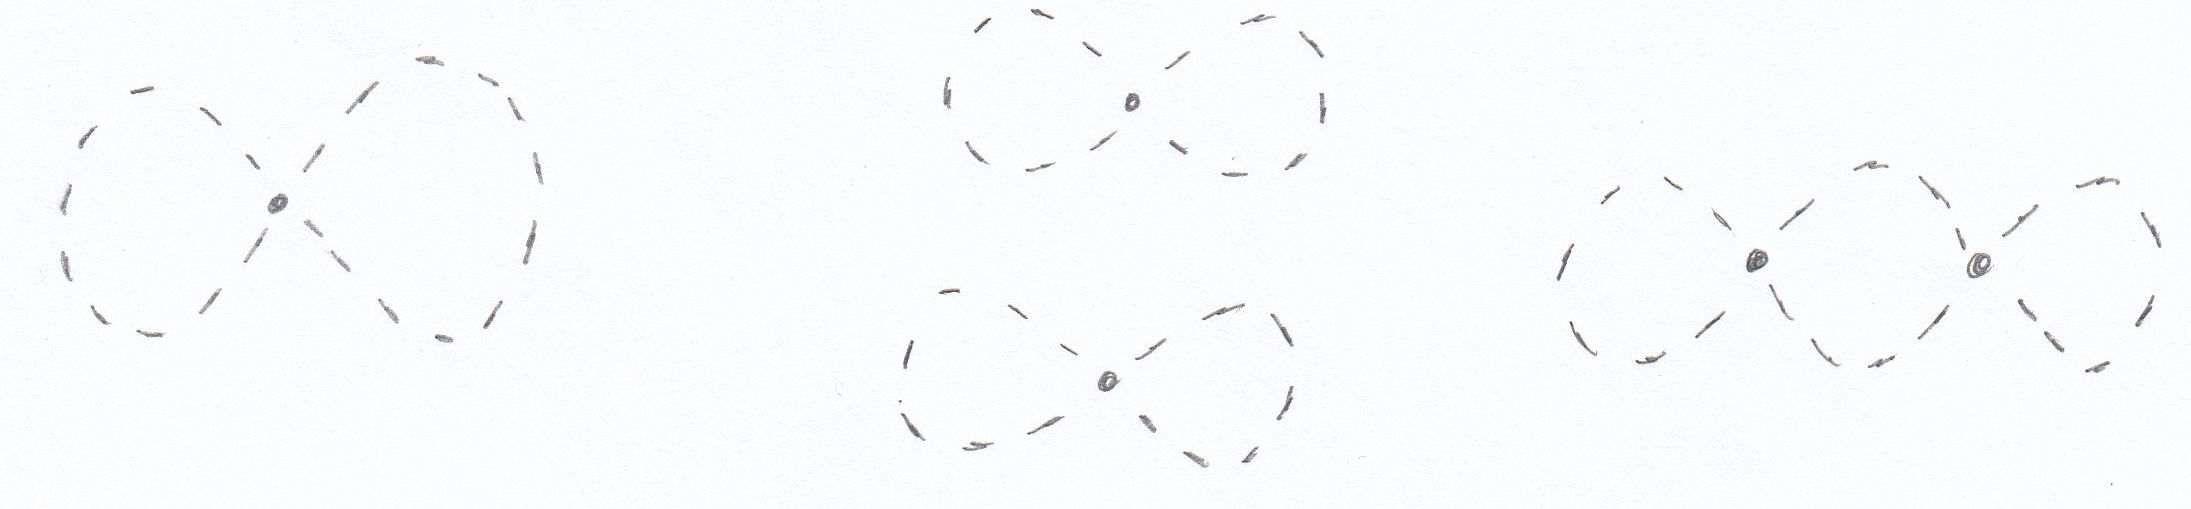
\includegraphics[width=0.6\textwidth]{figures/bub1}
		\end{figure}
		These diagrams do however also enter in the nominator, since what I have considered is only what can be measured. In practice all these vacuum diagrams can be added to the diagram describing the interaction cf.
		\begin{figure}[H]
			\captionsetup{width=1\textwidth}
			\centering
			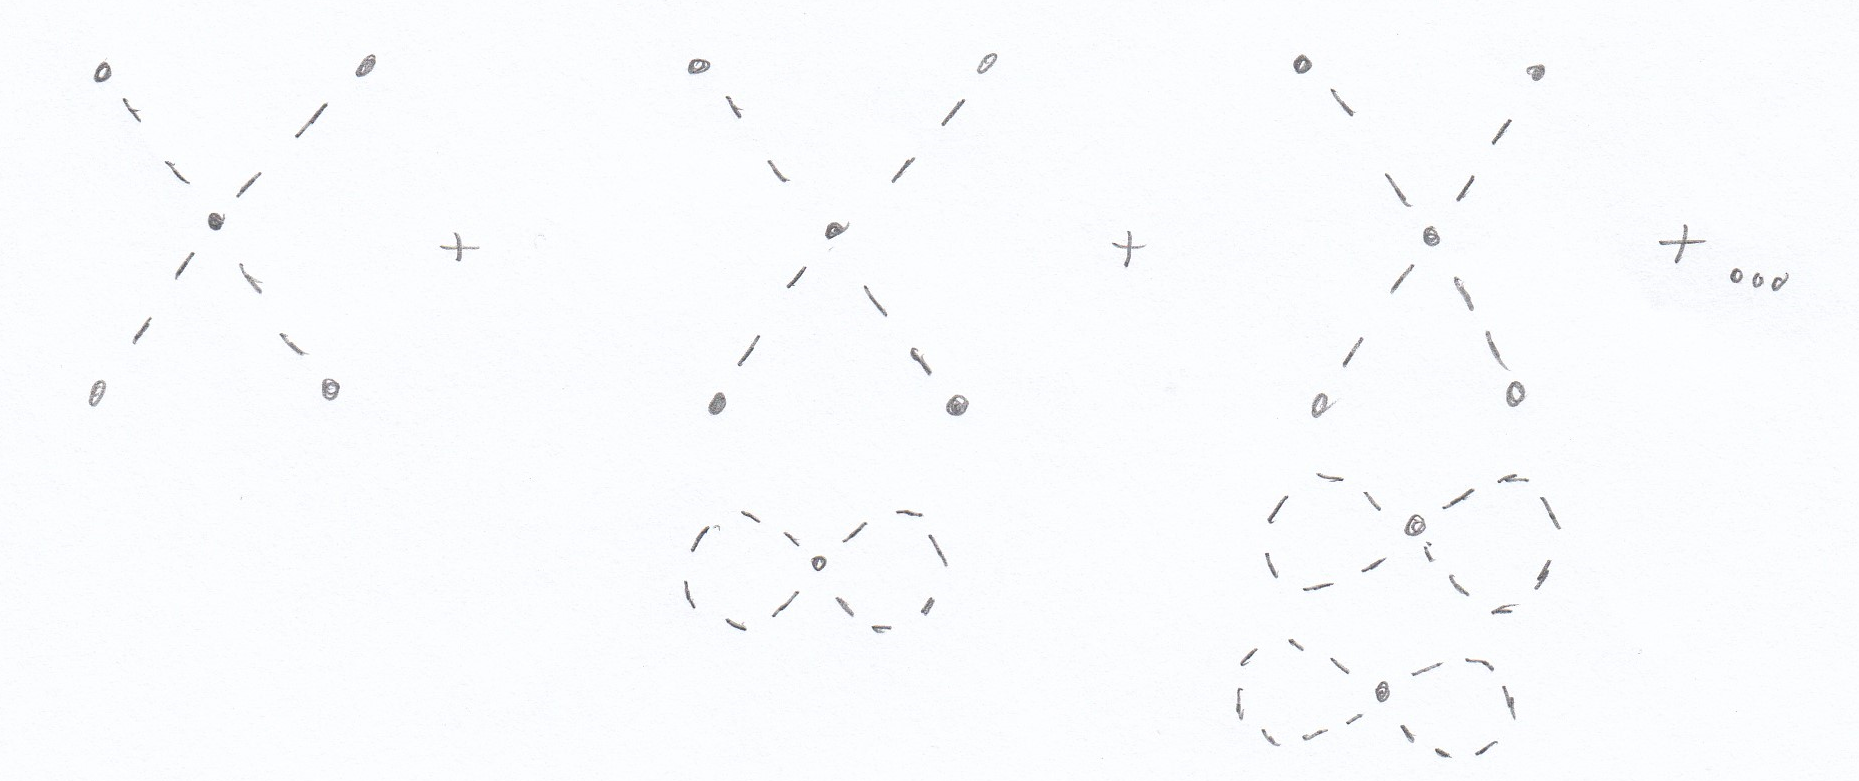
\includegraphics[width=0.6\textwidth]{figures/bub2}
		\end{figure}
		Hence, the fraction in the LSZ formula will be on the form
		\begin{figure}[H]
			\captionsetup{width=1\textwidth}
			\centering
			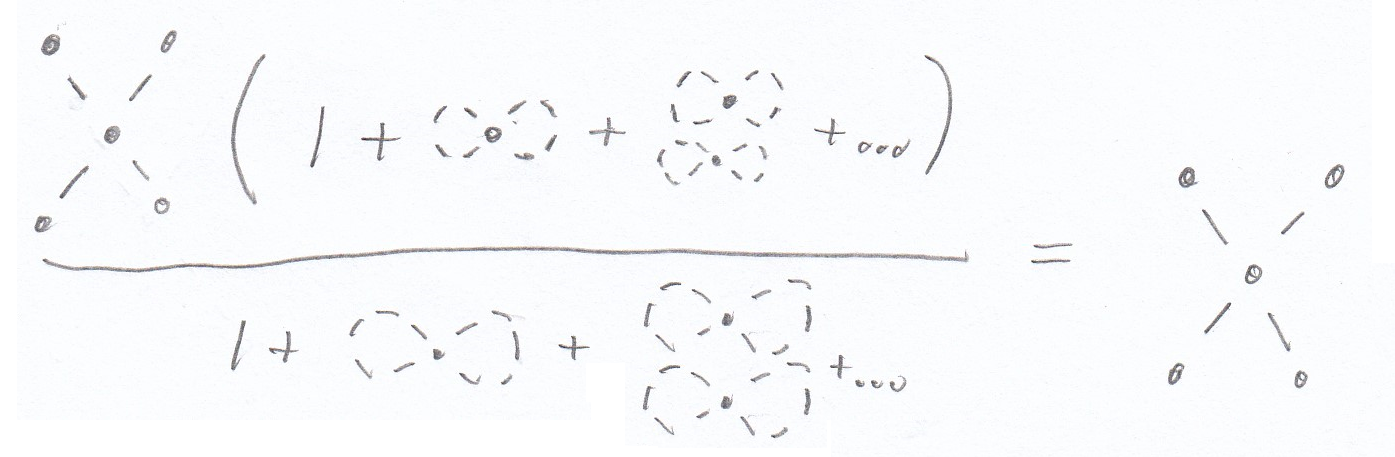
\includegraphics[width=0.6\textwidth]{figures/bub3}
		\end{figure}
		So, I can omit the vacuum diagrams in the denominator if I only consider diagrams with external particles. Hereby, I find
		\begin{equation}
			\braket{\vec{p'}_1\vec{p'}_2|iT|\vec{p}_1\vec{p}_2}=-i\lambda (2\pi)^4\delta^{(4)}(p'_1+p'_2-p_1-p_2).
		\end{equation} 
		From which it is clear that $i\mathcal{M}=-i\lambda$.
		
		\item \emph{Consider now a theory with $\mathcal{H}_I=\frac{\lambda}{3!}\phi^3$. What is the first non-vanishing term for this theory? Draw the relevant Feynman diagram.}
		
		The $\mathcal{O}(\lambda^0)$ term vanishes for the same reason that the $\mathcal{O}(\lambda^0)$ term for $\phi^4$-theory vanished; there is no interaction to zeroth order. The $\mathcal{O}(\lambda^1)$-term will however also vanish because the VEV will be on the form
		\begin{equation}
			VEV=\braket{0|T\{\phi(x_1)\phi(x_2)\phi(x_3)\phi(x_4)\phi^3(x)\}|0}.
		\end{equation} 
		Since the number of fields is uneven, not all fields can be contracted at the same time and so the VEV will be zero. Recall that this is because Wicks theorem is used to go from a time-ordered sequence of operators to a normal-ordered series. The normal-ordered terms will be zero if not all fields are contracted. Contracted fields make up a complex number that can go outside the VEV, but if there are uncontracted terms they will stay inside the VEV, and since the field is normal-ordered, the annihilation operator will be all the way to the right and annihilate onto the vacuum to make the terms vanish. Because of the previous arguments, the first non-vanishing order will be $\mathcal{O}(\lambda^2)$. Here, there will be connected terms and the number of fields will be $10$ (even), so all terms can be contracted at the same time. 
		Regarding the diagram; the previous procedure can be repeated to find the diagram, or alternatively the Feynman rules can be used. For each factor of $(-i\lambda)$ there is a vertex, where there, in this case, will be three joining lines. Hence
		\begin{figure}[H]
			\captionsetup{width=1\textwidth}
			\centering
			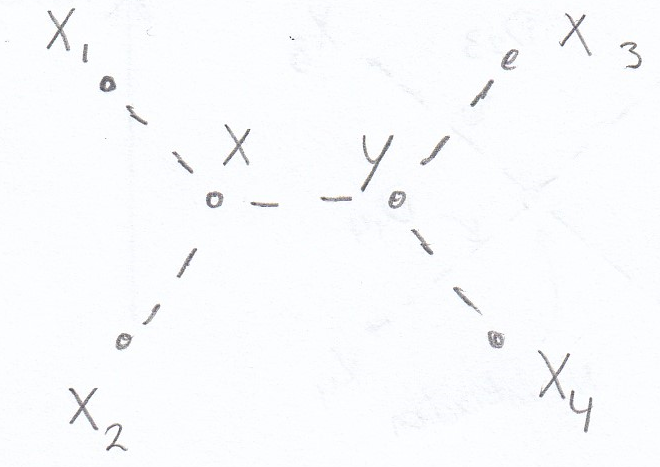
\includegraphics[width=0.4\textwidth]{figures/scal2}
		\end{figure}
		Again the vacuum diagrams will cancel. There are however other diagrams possible with two vertices:
		\begin{figure}[H]
			\captionsetup{width=1\textwidth}
			\centering
			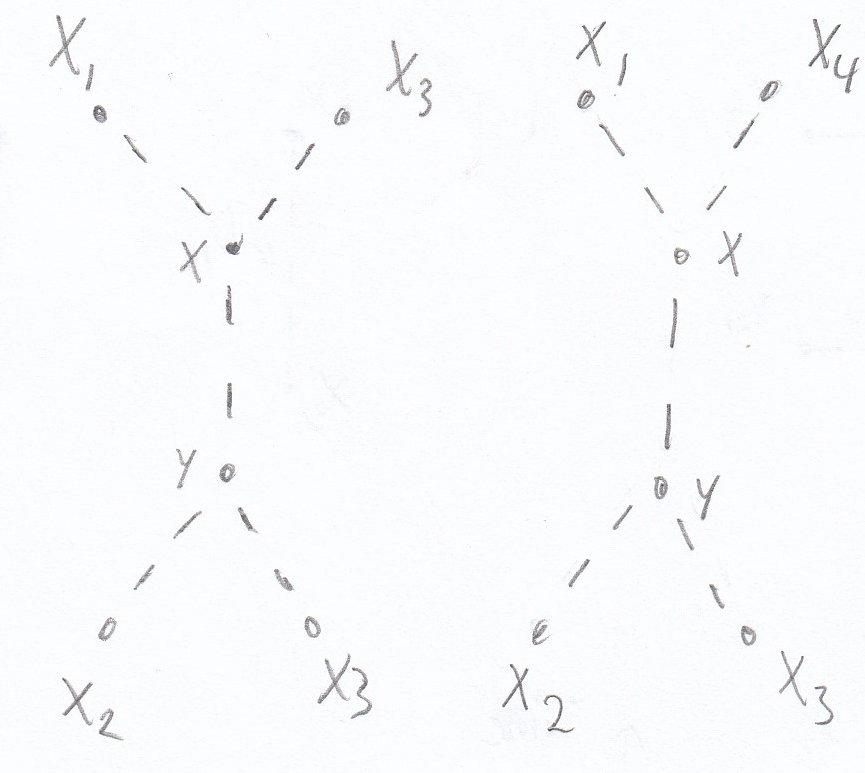
\includegraphics[width=0.3\textwidth]{figures/scal3}
		\end{figure}
		These are all the possible diagrams to leading order - Since $x_i$ has been connected to all $x_j's$. From the Feynman rules the matrix element can be found rather quickly.
		
	\end{enumerate}
	
\end{example}

\begin{example}
	\emph{Determine the lowest non-vanishing order of perturbation theory in Compton scattering.}\newline
	
	Compton scattering is an inelastic scattering between a photon and an electron,  i.e.
	\begin{equation}
		e^-(p_1)+\gamma(p_2)\Rightarrow e^-(p'_1)+\gamma(p'_2).
	\end{equation} 
	From equation \eqref{S4} the amplitude is given by
	\begin{equation}
		\begin{split}
			\mathcal{A}&=\braket{\vec{p'}_2,\vec{p'}_1|S|\vec{p}_2, \vec{p}_1}\\
			&=\braket{\vec{p'}_2,\vec{p'}_1|T\big\{1-i\int d^4x\mathcal{H}_I(x)+\frac{(-i)^2}{2!}\int d^4x_1\int d^4 x_2\mathcal{H}_I(x_2)\mathcal{H}_I(x_1)+...\big\}|\vec{p}_2, \vec{p}_1}.\\
		\end{split}
		\label{he}
	\end{equation} 
	The Hamiltonian density, $\mathcal{H}_I$, is given by
	\begin{equation}
		\mathcal{H}_{I}(x)=-|e|\bar{\psi}(x)\gamma^\mu\psi(x)A_\mu(x).
		\label{Hi}
	\end{equation} 
	The initial and final states are taken to be different and so $\braket{\vec{p'}_2,\vec{p'}_1|\vec{p}_2, \vec{p}_1}=0$. To evaluate the  time-ordered product use Wick's theorem. Wick's theorem relates the time-ordered product ($T\{...\}$) of a sequence of field operators to the normal-ordered product ($N\{...\}$). In mathematical form Wick's theorem\index{Wicks theorem} is given by
	\begin{equation}
		T\{...\}=N\{...+\text{All contractions}\}.
	\end{equation} 
	where "all contractions" refers to all contractions between the operators that the time ordering operator acts upon. The time ordering operator lists the contents with the latest entry farthest to the left whereas the normal ordering operator lists all the annihilation operators, belonging to the fields, to the right. Hence, the vacuum expectation value (VEV) of a normal ordered product is zero - since the annihilation operator acting on the vacuum is zero. Because the contraction between two field-operators is just a complex number, it can be moved outside the normal ordering operator. For this reason, only terms in which all field operators are contracted to another field operator contributes to the VEV. This leads to the important conclusion, that the number of fields must be an even number if there is to be any contribution from a given order of the perturbation theory. If the number of fields are uneven, it is not possible to contract all fields in a term, and the VEV will be zero. Because the number of fields vary with the order of the perturbation series, the leading order is the first order above zero which does not have an uneven number of fields. An important point here is that the number of fields is not the number of fields given in the interaction Hamiltonian density! There are extra fields stemming from the particle in the states involved (i.e. the initial and final states). These fields can be "pulled" out of the states (final and initial) by inserting the appropriate ladder operator, the vacuum state and a normalization factor. There are several different ways to explain, and do, this, but the point to remark here is that there appears an extra field for each final and initial particle involved in the process. Since there, for Compton scattering, are two particles, in both the initial and final state, the total number of fields is 4 plus what comes from the interaction Hamiltonian density. At $\mathcal{O}(i)$ there are three fields from the interaction Hamiltonian density, which results in seven fields in total, and so the contribution from this order vanishes. The leading order for Compton scattering is therefore $\mathcal{O}(i^2)$ (where there are 10 fields). 
	
\end{example}

\begin{example}
	\emph{Determine the invariant matrix element for Compton scattering via the Feynman rules.} \newline
	
	From considering the interaction Hamiltonian density of equation \eqref{Hi} it is clear that the vertices of QED will be of three particles; two fermions and one photon.	As seen in the previous example the leading order for Compton scattering, and QED scattering in general, is $\mathcal{O}(i^2)$. Since the number of vertices follow the order of perturbation theory there will be two vertices. Hence, the relevant diagrams will have two vertices to each of which two fermions and one photon will be attached. There are two diagrams fulfilling the requirements:
	\begin{center}
		\feynmandiagram [large, baseline=(b), vertical=a to b] {
			i1 [particle=\(\gamma\)] -- [photon, rmomentum'=\(p'_2\)] a -- [fermion, edge label'=\(p'_1\)] i2 [particle=\(e^{-}\)],
			a -- [anti fermion,edge label=\(p_1+p_2\)] b,
			f1 [particle=\(\gamma\)] -- [photon, momentum=\(p_2\)] b -- [anti fermion,edge label=\(p_1\)] f2 [particle=\(e^{-}\)],
		}; \qquad
		\feynmandiagram [large ,baseline=(b), horizontal=a to b] {
			i1 [particle=\(\gamma\)] -- [photon, momentum'=\(p_2\)] a -- [fermion,edge label'=\(p'_1\)] i2 [particle=\(e^{-}\)],
			a -- [anti fermion ,edge label=\(p_1-p'_2\)] b,
			f1 [particle=\(e^{-}\)] -- [fermion, edge label=\(p_1\)] b -- [photon,, momentum=\(p'_2\)] f2 [particle=\(\gamma\)],
		};
	\end{center}
	where the direction of time is upwards. In order to write down the invariant matrix element from the Feynman diagrams, use the following procedure; at each side of the propagator is go towards the fermion current and use the feynman rules, then insert the propagator and go towards the fermion current on the other side of the propagator. Naming the vertices in the process means
	\begin{equation}
		\begin{split}
			i\mathcal{M}_{vertical}&=\bar{u}^{s'}(\vec{p'}_1)(-iQ\gamma^\mu)\epsilon^{(\lambda')*}_{\mu}(\vec{p'}_2)\frac{i(\slashed p_1+\slashed p_2+m)}{(p_1+p_2)^2-m^2}\epsilon^{(\lambda)}_{\rho}(\vec{p}_2)(-iQ\gamma^\rho)
			u^s(\vec{p}_1)\\
			&=-i|e|^2\epsilon^{(\lambda')*}_{\mu}(\vec{p'}_2)\epsilon^{(\lambda)}_{\rho}(\vec{p}_2)\frac{\bar{u}^{s'}(\vec{p'}_1)\gamma^\mu(\slashed p_1+\slashed p_2+m)\gamma^\rho u^s(\vec{p}_1)}{(p_1+p_2)^2-m^2},
		\end{split}
		\label{M1}
	\end{equation} 
	\begin{equation}
		\begin{split}
			i\mathcal{M}_{horizontal}&=\bar{u}^{s'}(\vec{p'}_1)(-iQ\gamma^\mu)\epsilon^{(\lambda)}_{\mu}(\vec{p}_2)\frac{i(\slashed p_1-\slashed p'_2+m)}{(p_1-p'_2)^2-m^2}\epsilon^{(\lambda')*}_{\rho}(\vec{p'}_2)(-iQ\gamma^\rho)
			u^s(\vec{p}_1)\\
			&=-i|e|^2\epsilon^{(\lambda)}_{\mu}(\vec{p}_2)\epsilon^{(\lambda')*}_{\rho}(\vec{p'}_2)\frac{\bar{u}^{s'}(\vec{p'}_1)\gamma^\mu(\slashed p_1-\slashed p'_2+m)\gamma^\rho
				u^s(\vec{p}_1)}{(p_1-p'_2)^2-m^2}.
		\end{split}
		\label{M2}
	\end{equation} 
	
\end{example}


\begin{example}
	\emph{Determine the invariant matrix element for Compton scattering in position space.}\newline
	
	Position space refers to the analog of the LSZ formula. However, instead of re-deriving the LSZ formula for QED it is convenient to use a slightly different approach. Using that the lowest non-vanishing order for QED is $\mathcal{O}(i^2)$, alongside the fact that if the zeroth order is neglected in the expansion of the $S$-matrix; $\mathcal{A}\Rightarrow \braket{\dots'|iT|\dots}$, equation \eqref{he} can be written viz
	\begin{equation}
		\begin{split}
			\braket{\vec{p'}_2,\vec{p'}_1|iT|\vec{p}_2, \vec{p}_1}&=\frac{(i)^2|e|^2}{2!}\int d^4x_1\int d^4 x_2\braket{\vec{p'}_2,\vec{p'}_1|T\big\{\mathcal{H}_I(x_2)\mathcal{H}_I(x_1)\}|\vec{p}_2,\vec{p}_1},\\
		\end{split}
		\label{t1}
	\end{equation} 
	where
	\begin{equation}
		\mathcal{H}_I(x_2)\mathcal{H}_I(x_1)=\bar{\psi}(x_1)\gamma^\mu\psi(x_1)A_\mu(x_1)\bar{\psi}(x_2)\gamma^\nu\psi(x_2)A_\nu(x_2).
	\end{equation} 
	To evaluate equation \ref{t1} use Wick's theorem\index{Wicks theorem}. From Wick's theorem the time-ordering of a product of field operators, sandwiched between two states, can be written as the normal ordered product of all possible contractions between the field operators. To determine which terms should enter the sum, use the definitions of the different contractions
	\begin{equation}
		\begin{split}
			&\contraction{0}{\psi}{(x_1)}{\psi}
			\psi(x_1)\psi(x_2)=0 \\
			&\contraction{0}{\bar{\psi}}{(x_1)}{\bar{\psi}}
			\bar{\psi}(x_1)\bar{\psi}(x_2)=0\\
			&\contraction{0}{\psi}{(x_1)}{\bar{\psi}}
			\psi(x_1)\bar{\psi}(x_2)=iS_F(x_1-x_2)=\int\frac{d^4q}{(2\pi)^4}\frac{i(\slashed q+m)e^{-iq\cdot(x_1-x_2)}}{q^2-m^2}\\
			&\contraction{0}{\psi}{(x_i)}{\vec{p}_1}
			\psi(x_i)\ket{\vec{p}_1}\,\,=\int\frac{d^3q}{(2\pi)^3}\frac{1}{\sqrt{2E_{\vec{q}}}}\sum_{s'}\big(u^{s'}(\vec{q})e^{-iq\cdot x_i}a^{s'}_{\vec{q}}+v^{s'}(\vec{q})e^{iq\cdot x_i}b^{s'\dagger}_{\vec{q}}\big)\sqrt{2E_{\vec{p}_1}}\,a^{s\dagger}_{\vec{p}_1}\ket{0}\\
			&\qquad\qquad=\int\frac{d^3q}{(2\pi)^3}\frac{1}{\sqrt{2E_{\vec{q}}}}\sum_{s'}u^{s'}(\vec{q})e^{-iq\cdot x_i}a^{s'}_{\vec{q}}\sqrt{2E_{\vec{p}_1}}\,a^{s\dagger}_{\vec{p}_1}\ket{0}\\
			&\qquad\qquad=\int\frac{d^3q}{(2\pi)^3}\frac{\sqrt{2E_{\vec{p}_1}}}{\sqrt{2E_{\vec{q}}}}\sum_{s'}u^{s'}(\vec{q})e^{-iq\cdot x_i}\big(a^{s\dagger}_{\vec{p}_1}a^{s'}_{\vec{q}}+(2\pi)^3\delta^{(3)}(\vec{q}-\vec{p}_1)\delta_{s,s'}\big)\ket{0}\\
			&\qquad\qquad=u^{s}(\vec{p}_1)e^{-ip_1\cdot x_i}\ket{0}=\text{fermion, initial state}.
		\end{split}
	\end{equation} 
	From similar calculations
	\begin{equation}
		\contraction{0}{\psi}{(x_i)}{\vec{p}_1}
		\bar{\psi}(x_i)\ket{\vec{p}_1}=\bar{v}^s(p)e^{-ip\cdot x}\ket{0}=\text{anti fermion, initial state}.
	\end{equation} 
	In the case of the bra-contractions the other field operator is used
	\begin{equation}
		\begin{split}
			\contraction{0}{\vec{p'}_1}{\psi}{(x}
			\bra{\vec{p'}_1}\psi(x_i)&=\bra{0}b^{s}_{\vec{p'}_1}\sqrt{2E_{\vec{p'}_1}}\int\frac{d^3q}{(2\pi)^3}\frac{1}{\sqrt{2E_{\vec{q}}}}\sum_{s'}\big(u^{s'}(\vec{q})e^{-iq\cdot x_i}a^{s'}_{\vec{q}}+v^{s'}(\vec{q})e^{iq\cdot x_i}b^{s'\dagger}_{\vec{q}}\big)\\
			&=\int\frac{d^3q}{(2\pi)^3}\frac{\sqrt{2E_{\vec{p'}_1}}}{\sqrt{2E_{\vec{q}}}}\sum_{s'}\bra{0}b^{s}_{\vec{p'}}b^{s'\dagger}_{\vec{q}}v^{s'}(\vec{q})e^{iq\cdot x_i}\\
			&=\int\frac{d^3q}{(2\pi)^3}\frac{\sqrt{2E_{\vec{p'}_1}}}{\sqrt{2E_{\vec{q}}}}\sum_{s'}v^{s'}(\vec{q})e^{iq\cdot x_i}\bra{0}\big(b^{s'\dagger}_{\vec{q}}b^{s}_{\vec{p'}}+(2\pi)^3\delta^{(3)}(\vec{q}-\vec{p'}_1)\delta_{s,s'})\big)\\
			&=\bra{0}v^{s'}(\vec{p'}_1)e^{ip'_1\cdot x_i}=\text{anti fermion, final state}.
		\end{split}
	\end{equation} 
	Similarly
	\begin{equation}
		\contraction{0}{\vec{p'}_1}{\psi}{(x_i)}
		\bra{\vec{p'}_1}\bar{\psi}(x_i)=\bra{0}\bar{u}^{s'}(\vec{p'}_1)e^{ip'_1\cdot x_i}=\text{fermion, final state}.
	\end{equation} 
	Lastly, for the photons the possible contractions are
	\begin{equation}
		\begin{split}
			\contraction{0}{\psi}{(x_i),}{\vec{p}}
			A_\mu(x_i)\ket{\vec{p}_2}&=\int\frac{d^3q}{(2\pi)^3}\frac{1}{\sqrt{2E_{\vec{q}}}}\sum_{r}\big(\varepsilon^{r}_\mu(\vec{q})e^{-iq\cdot x_i}a^{r}_{\vec{q}}+\varepsilon^{r*}_\mu(\vec{q})e^{iq\cdot x_i}a^{r\dagger}_{\vec{q}}\big)\sqrt{2E_{\vec{p}_2}}\,a^{s\dagger}_{\vec{p}_2}\ket{0}\\
			&=\int\frac{d^3q}{(2\pi)^3}\frac{\sqrt{2E_{\vec{k}}}}{\sqrt{2E_{\vec{q}}}}\sum_{r}\varepsilon^{r}_\mu(\vec{q})e^{-iq\cdot x_i}a^{r}_{\vec{q}}\,a^{s\dagger}_{\vec{p}_2}\ket{0}\\
			&=\int\frac{d^3q}{(2\pi)^3}\frac{\sqrt{2E_{\vec{p}_2}}}{\sqrt{2E_{\vec{q}}}}\sum_{r}\varepsilon^{r}_\mu(\vec{q})e^{-iq\cdot x_i}\big(a^{s\dagger}_{\vec{k}}\,a^{r}_{\vec{q}}+(2\pi)^3\delta^{(3)}(\vec{q}-\vec{p}_2)\delta_{s,r}\big)\ket{0}\\
			&=\varepsilon_\mu^r(\vec{p}_2) e^{-ip_2\cdot x_i}\ket{0}.\\
		\end{split}
	\end{equation} 	
	Likewise
	\begin{equation}
		\begin{split}
			\contraction{0}{\vec{p'}}{\psi}{(x}
			\bra{\vec{p'_2}}A_\mu(x_i)=\bra{0}\varepsilon_\mu^{r'*}(\vec{p'}_2) e^{ip'_2\cdot x_i}.\\
		\end{split}
	\end{equation} 
	With the contractions defined as above Wick's theorem can be used to significantly simplify equation \ref{t1}. From Wick's theorem all terms must be contracted to contribute. Further more, contractions between $A$ an the other fields are zero, just as contractions among $\psi$'s and $\bar{\psi}$'s. Hence, to contribute there must be terms on the form
	\begin{equation}
		\contraction{0}{\psi}{,,,}{\bar{\psi}}
		\psi(x_1)\bar{\psi}(x_2), \quad \contraction{0}{\psi}{,,,}{\vec{p}}
		\psi(x_i)\ket{\vec{p}}, \quad \contraction{0}{\vec{p'}}{0}{(x_i)}
		\bra{\vec{p'}}\bar{\psi}(x_i), \quad 	\contraction{0}{\vec{p'}}{\psi}{(x}
		\bra{\vec{k'}}A_\mu(x_i), \quad \contraction{0}{\psi}{(x_i),}{\vec{p}}
		A_\mu(x_i)\ket{\vec{k}}.
	\end{equation} 
	There are four terms like this. Defining $I\equiv \braket{\vec{p'}_2,\vec{p'}_1|T\big\{\mathcal{H}_I(x_2)\mathcal{H}_I(x_1)\}|\vec{p}_2,\vec{p}_1}$
	\begin{equation}
		\begin{split}
			\contraction{I=N\big\{,}{\vec{p'}}{,,,\vec{k'}|}{\bar{\psi}}
			\contraction{,,,I=N\vec{p'},\vec{k'}|\bar{\psi}(x_1)\gamma^\mu}{,,\psi(x_1)}{A_\mu(x_1)}{\bar{\psi}(x_2)}
			\contraction{,,,,,,,,,,,,,,,,,,,,,,,,,,,,,,,,,,,,,,,,,,,}{\psi(x_2)}{,A_\nu(x_2)|}{\vec{p}}
			\contraction[2ex]{,,,,,,,,,,,,}{\vec{k'}}{,,,,,,,,,,,,,}{A_\mu(x_1)}
			\contraction[2ex]{,,,,.,,,,,,,,,,,,,,,,,,,,,,,,,,,,,,,,,,,,,,,,,,,}{A_\nu(x_2)}{,,,,,,}{\vec{k}}
			I&=N\big\{\braket{\vec{p'}_1,\vec{p'}_2|\bar{\psi}(x_1)\gamma^\mu\psi(x_1)A_\mu(x_1)\bar{\psi}(x_2)\gamma^\nu\psi(x_2)A_\nu(x_2)|\vec{p}_1,\vec{p}_2}\\
			&\qquad
			\contraction{,,,,}{\vec{p'}}{,,,\vec{k'}|}{\bar{\psi}}
			\contraction{,,,,,,,,,,,,,,,,,}{\psi(x_1)}{A_\mu(x_1)}{\bar{\psi}(x_2)}
			\contraction{,,,,,,,,,,,.,,,,,,,,,,,,,,,,,,,,,,,,,,}{\psi(x_2)}{,A_\nu(x_2)|}{\vec{p}}
			\contraction[3ex]{,,,,,.,}{\vec{k'}}{,,,,,,,,,,,,,,,,,,,,,,,,,,,,,,,,,}{A_\mu(x_2)}
			\contraction[2ex]{,,,,,,,,,,,,,,,,,,,,,,}{A_\nu(x_1)}{,,,,,,,,,,,,,,,,,,,,,,,,,}{\vec{k}}
			+\braket{\vec{p'}_1,\vec{p'}_2|\bar{\psi}(x_1)\gamma^\mu\psi(x_1)A_\mu(x_1)\bar{\psi}(x_2)\gamma^\nu\psi(x_2)A_\nu(x_2)|\vec{p}_1,\vec{p}_2}\\
			&\qquad
			\contraction{,,,,}{\vec{p'}}{,,,,,.,,,,,,,,,,,,,,,,,,}{\bar{\psi}(x_2)}
			\contraction[5ex]{,,,,,,,,,}{\bar{\psi}(x_1)}{,,,,,,,,,,,,,,,,,,,,,,,,}{\psi(x_2)}
			\contraction[4ex]{,,,,,,,,,,,,,,,,,}{\psi(x_1)}{,,,,,,,,,,,,,,,,,,,,,,,,,,,,,,}{\vec{p}}
			\contraction[3ex]{,,,,,.,,}{\vec{k'}}{,,,,,,,,,,,.,,,,,,,,,,,,,,,,,,,,,,}{A_\mu(x_2)}
			\contraction[2ex]{,,,,,.,,,,,,,,,,,,,,,,,}{A_\nu(x_1)}{,,,,,,,,,,,,,,,,,,,,,,,,,}{\vec{k}}
			+\braket{\vec{p'}_1,\vec{p'}_2|\bar{\psi}(x_1)\gamma^\mu\psi(x_1)A_\mu(x_1)\bar{\psi}(x_2)\gamma^\nu\psi(x_2)A_\nu(x_2)|\vec{p}_1,\vec{p}_2}\\	
			&\qquad
			\contraction{,,,,}{\vec{p'}}{,,,,.,,,,,,,,,,,,,,,,,,,}{\bar{\psi}(x_2)}
			\contraction[3ex]{,,,,,.,,,}{\bar{\psi}(x_1)}{,,,,,,,,,,,,,,,,,,,,,,,}{\psi(x_2)}
			\contraction[2ex]{,,,,,,,,,,,,,,,,,}{\psi(x_1)}{,,,,,,,,,,,,,,,,,,,,,,,,,,,,,}{\vec{p}}
			\contraction{,,,,,,,,,,,,,,,,,,,,,,,,,,,,,,,,,,,,,,,,,,,,}{\psi(x_2)}{,,,,,}{\vec{p}}
			\contraction[4ex]{,,,.,,,,}{\vec{k'}}{,,,,,,,,,,,,,}{A_\mu(x_1)}
			+\braket{\vec{p'}_1,\vec{p'}_2|\bar{\psi}(x_1)\gamma^\mu\psi(x_1)A_\mu(x_1)\bar{\psi}(x_2)\gamma^\nu\psi(x_2)A_\nu(x_2)|\vec{p}_1,\vec{p}_2}\big\}.\\
		\end{split}
		\label{I}
	\end{equation} 
	There are two different fermion terms and two different photon terms. The two different fermion terms are in fact identical. This can be seen as follows
	\begin{equation}
		\begin{split}
			\contraction{,,,,}{\vec{p'}}{,,,,,,,,,,,,,,,,,,,,,,,,,\vec{k'}|}{\bar{\psi}}
			\contraction{.,,,,,,,,.,,,,,,,,,,,,,,,,,,,,,,,,,,,,,,,,,,,,,,,,,,,,,,,,,,,,,,,}{\vec{p'}}{,..,\vec{k'}|}{\bar{\psi}}
			N\{[\bar{\psi}(x_1)\slashed A(x_1)\psi(x_1)][\bar{\psi}(x_2)\slashed A(x_2)\psi(x_2)]\}&=(-1)^4N\{[\bar{\psi}(x_2)\slashed A(x_2)\psi(x_2)][\bar{\psi}(x_1)\slashed A(x_1)\psi(x_1)]\}\\
			&\contraction{,,,,,,,,,,,,,,,,,,}{\vec{p'}}{,,,\vec{k'}|}{\bar{\psi}}
			=N\{[\bar{\psi}(x_1)\slashed A(x_1)\psi(x_1)][\bar{\psi}(x_2)\slashed A(x_2)\psi(x_2)]\}.
		\end{split}
	\end{equation} 	
	Hereby
	\begin{equation}
		\begin{split}
			I&=2\bar{u}^{s'}(\vec{p'}_1)\gamma^\mu iS_{F}(x_1-x_2)\gamma^\nu u^s(\vec{p}_1)e^{ip'_1\cdot x_1}e^{-ip_1\cdot x_2}N\{\braket{\vec{p'}_2|A_\mu(x_1)A_\nu(x_2)|\vec{p}_2}\}.
		\end{split}
	\end{equation} 
	The $A's$ can each couple to either the initial or final state, so
	\begin{equation}
		\begin{split}
			N\{\braket{\vec{p'}_2|A_\mu(x_1)A_\nu(x_2)|\vec{p}_2}\}=\varepsilon_\mu^{r'*}(\vec{p'}_2)\varepsilon_\nu^{r}(\vec{p}_2)e^{ip'_2\cdot x_1}e^{-ip_2\cdot x_2}+\varepsilon_\nu^{r'*}(\vec{p'}_2)\varepsilon_\mu^{r}(\vec{p}_2)e^{ip'_2\cdot x_2}e^{-ip_2\cdot x_1}.
		\end{split}
	\end{equation} 
	Hereby
	\begin{footnotesize}
	 \begin{equation}
		\begin{split}
			\braket{\vec{p'}_1,\vec{p'}_2|i\hat{T}|\vec{p}_1, \vec{p}_2}&=i(i)^2|e|^2\\
			&\quad \cdot\bigg(\int d^4x_1\int d^4x_2
			\bar{u}^{s'}(\vec{p'}_1)\gamma^\mu S_{F}(x_1-x_2)\gamma^\nu u^s(\vec{p}_1)e^{ip'_1 x_1}e^{-ip_1 x_2}\varepsilon_\mu^{r'*}(\vec{p'}_2)\varepsilon_\nu^{r}(\vec{p}_2)e^{ip'_2 x_1}e^{-ip_2 x_2}\\
			&\quad\quad\quad+\int d^4x_1\int d^4x_2
			\bar{u}^{s'}(\vec{p'}_1)\gamma^\mu S_{F}(x_1-x_2)\gamma^\nu u^s(\vec{p}_1)e^{ip'_1 x_1}e^{-ip_1x_2}
			\varepsilon_\nu^{r'*}(\vec{p'}_2)\varepsilon_\mu^{r}(\vec{p}_2)e^{ip'_2x_2}e^{-ip_2 x_1}\bigg)\\
			&\equiv-i|e|^2\sum_{i=1}^{2}T_i.
		\end{split}
		\label{t2}
	\end{equation} 
\end{footnotesize}	
	Considering each of the terms
	\begin{footnotesize}
	 \begin{equation}
		\begin{split}
			&T_1=\int d^4x_1\int d^4
			\bar{u}^{s'}(\vec{p'}_1)\gamma^\mu S_{F}(x_1-x_2)\gamma^\nu u^s(\vec{p}_1)e^{ip'_1 x_1}e^{-ip_1 x_2}\varepsilon_\mu^{r'*}(\vec{p'}_2)\varepsilon_\nu^{r}(\vec{p}_2)e^{ip'_2 x_1}e^{-ip_2 x_2}\\
			&\quad=\int \frac{d^4q}{(2\pi)^4}
			\bar{u}^{s'}(\vec{p'}_1)\gamma^\mu \frac{\slashed q+m}{q^2-m^2}\gamma^\nu u^s(\vec{p}_1)\varepsilon_\mu^{r'*}(\vec{p'}_2)\varepsilon_\nu^{r}(\vec{p}_2)
			\underbrace{\int d^4x_1
				e^{ip'_2\cdot x_1}e^{ip'_1 x_1}e^{-iq x_1}}_{(2\pi)^4\delta^{(4)}(p'_2+p'_1-q)}
			\underbrace{\int d^4x_2
				e^{-ip_2 x_2}
				e^{-ip_1x_2}e^{iq x_2}}_{(2\pi)^4\delta^{(4)}(p_2+p_1-q)}\\
			&\quad=(2\pi)^4\delta^{(4)}(p'_2+p'_1-p_1-p_2)\bar{u}^{s'}(\vec{p'}_1)\gamma^\mu \frac{\slashed p_1+\slashed p_2+m}{(p_1+p_2)^2-m^2}\gamma^\nu u^s(\vec{p}_1)\varepsilon_\mu^{r'*}(\vec{p'}_2)\varepsilon_\nu^{r}(\vec{p}_2),\\
			&T_2=\int d^4x_1\int d^4x_2
			\bar{u}^{s'}(\vec{p'}_1)\gamma^\mu S_{F}(x_1-x_2)\gamma^\nu u^s(\vec{p}_1)e^{ip'_1 x_1}e^{-ip_1 x_2}
			\varepsilon_\nu^{r'*}(\vec{p'}_2)\varepsilon_\mu^{r}(\vec{p}_2)e^{ip'_2 x_2}e^{-ip_2 x_1}\\
			&\quad=\int \frac{d^4q}{(2\pi)^4}
			\bar{u}^{s'}(\vec{p'}_1)\gamma^\mu \frac{\slashed q+m}{q^2-m^2}\gamma^\nu u^s(\vec{p}_1)
			\varepsilon_\nu^{r'*}(\vec{p'}_2)\varepsilon_\mu^{r}(\vec{p}_2)
			\underbrace{\int d^4x_1
				e^{ip'_1 x_1}e^{-ip_2 x_1}e^{-iqx_1}}_{(2\pi)^4\delta^{(4)}(p'_1-p_2-q)}\underbrace{\int d^4x_2e^{-ip_1 x_2}
				e^{ip'_2 x_2}e^{iq x_2}}_{(2\pi)^4\delta^{(4)}(p_1-p'_2-q)}\\
			&\quad=(2\pi)^4\delta^{(4)}(p'_2+p'_1-p_1-p_2)\bar{u}^{s'}(\vec{p'}_1)\gamma^\mu \frac{\slashed p_1-\slashed p'_2+m}{(p'_1-p'_2)^2-m^2}\gamma^\nu u^s(\vec{p}_1)
			\varepsilon_\nu^{r'*}(\vec{p'}_2)\varepsilon_\mu^{r}(\vec{p}_2).
		\end{split}
		\label{t3}
	\end{equation}
	\end{footnotesize} 
	By combining equations \eqref{t2} and \eqref{t3}
	\begin{footnotesize}
	 \begin{equation}
		\begin{split}
			\braket{\vec{p'}_1,\vec{p'}_2|i\hat{T}|\vec{p}_1, \vec{p}_2}&=-i(2\pi)^4\delta^{(4)}(p'_2+p'_1-p_1-p_2)|e|^2\varepsilon_\nu^{r'*}(\vec{p'}_2)\varepsilon_\mu^{r}(\vec{p}_2)\\
			&\quad\cdot\bigg(\bar{u}^{s'}(\vec{p'}_1)\gamma^\mu \frac{\slashed p_1+\slashed p_2+m}{(p_1+p_2)^2-m^2}\gamma^\nu u^s(\vec{p}_1)+\bar{u}^{s'}(\vec{p'}_1)\gamma^\nu \frac{\slashed p_1-\slashed p'_2+m}{(p_1-p'_2)^2-m^2}\gamma^\mu u^s(\vec{p}_1)\bigg),
		\end{split}
		\label{t4}
	\end{equation}
	\end{footnotesize} 
	where the dummy indices ($\mu,\nu$) have been relabeled on the $\gamma's$ on the second term in order to factorize the $\epsilon's$. From equation \eqref{t4}
	 \begin{equation}
		\begin{split}
			i\mathcal{M}&=-i|e|^2\varepsilon_\nu^{r'*}(\vec{p'}_2)\varepsilon_\mu^{r}(\vec{p}_2)\\
			&\qquad\cdot\bigg(\bar{u}^{s'}(\vec{p'}_1)\gamma^\mu \frac{\slashed p_1+\slashed p_2+m}{(p_1+p_2)^2-m^2}\gamma^\nu u^s(\vec{p}_1)+\bar{u}^{s'}(\vec{p'}_1)\gamma^\nu \frac{\slashed p_1-\slashed p'_2+m}{(p_1-p'_2)^2-m^2}\gamma^\mu u^s(\vec{p}_1)\bigg).
		\end{split}
		\label{M3}
	\end{equation} 
	By comparison between equation \eqref{M3}, \eqref{M2} and \eqref{M1} it is clear that the same result is obtained as in the previous example where the invariant matrix element was written directly from the Feynman rules of QED.
	
\end{example}

\section{Effective field theory}
\index{Scattering, meson}
\index{Scattering, hadron}
Particle physics often consider scattering events between hadrons and mesons. The issue with such composite particles is that the amplitude written in terms of the Feynman rules does not apply unless the particles considered are free. Quarks confined in hadrons and mesons are not free (the majority of the hadron mass is made up of the gluon field produced by the quark) and further more; the underlying theory describing the behavior of the quarks (QCD) is non-perturbative. In such cases the Feynman rules cannot be used and as such the position space approach is used. It goes as follows; the interaction (the states evolve via the interaction Hamiltonian density, $\mathcal{H}_I$, which in turn is read off from the interacting part of the interaction Lagrangian density, $\mathcal{L}_I$) Lagrangian density is related to the amplitude for a scattering by using the definition of $S$ from equation \eqref{S} alongside equation \eqref{S1} through \eqref{S4}. Taking the states to be more general, eg. $\ket{p_1, A}$ for a particle scattering of a nucleus. $p_1$ denotes the momentum of the scattered particle whereas $A$ denotes the more complex state of the nucleus (eg. with momentum, spin,...) and using equation \eqref{S} in equation \eqref{S1} (and expanding the exponential)
\begin{equation}
	\begin{split}
		\mathcal{A}&=\braket{f|S|i}\\
		&=\braket{f|i}-i\int d^4x\braket{f|\mathcal{H}_I(x)|i}+\mathcal{O}(i^2),
	\end{split}
	\label{S5}
\end{equation} 
where $i$ denotes the initial state, $f$ denotes the final state and $\mathcal{H}_I(x)$ is the interaction Hamiltonian in the interaction picture. From equation \eqref{S4}
\begin{equation}
	\begin{split}
		\mathcal{A}&=\braket{f|i}+(2\pi)^4\delta^{(4)}(\Sigma p'-\Sigma p)i\mathcal{M}.
	\end{split}
	\label{S6}
\end{equation} 
By equating equation \eqref{S5} and \eqref{S6}
\begin{equation}
	(2\pi)^4\delta^{(4)}(\Sigma p'-\Sigma p)i\mathcal{M}=-i\int d^4x\braket{f|\mathcal{H}_I(x)|i} +\mathcal{O}(i^2).
	\label{S7}
\end{equation} 
Taking $p^\mu$ to be the space-time translation operator, the interaction Hamiltonian density can be written as follows
\begin{equation}
	\mathcal{H}_I(x)=e^{ipx}\mathcal{H}_{I}(0)e^{-ipx}.
	\label{S8}
\end{equation} 
By applying equation \eqref{S8} in equation \eqref{S7}
\begin{equation}
	\begin{split}
		(2\pi)^4\delta^{(4)}(\Sigma p'-\Sigma p)\mathcal{M}&=-\int d^4x\braket{f|e^{ipx}\mathcal{H}_I(0)e^{-ipx}|i}+\mathcal{O}(i^2)\\
		&=-\int d^4xe^{-i(\Sigma p-\Sigma p')x} \braket{f|\mathcal{H}_I(0)|i}+\mathcal{O}(i^2)\\
		&=-(2\pi)^4\delta^{(4)}(\Sigma p'-\Sigma p) \braket{f|\mathcal{H}_I(0)|i}+\mathcal{O}(i^2).\\
	\end{split}
	\label{S9}
\end{equation} 
From equation \eqref{S9} it is clear that
\begin{equation}
	\mathcal{M}=-\braket{f|\mathcal{H}_I(0)|i}+\mathcal{O}(i^2).
\end{equation} 
If the interaction Lagrangian does not contain derivatives, then $-\mathcal{L}_I(0)=\mathcal{H}_I(0)$. Hereby
\begin{equation}
	\mathcal{M}=\braket{f|\mathcal{L}_I(0)|i}+\mathcal{O}(i^2).
	\label{S10}
\end{equation} 
$\mathcal{L}_I(0)$ can then be described by an effective Lagrangian density\index{Fermi Lagrangian}. An effective Lagrangian density is a Lagrangian density that is proportional to product of the two currents of the interaction. The effective Lagrangian density is valid only in the limit in which the momentum of the mediator squared goes to zero, i.e. $q^2\Rightarrow 0$. In the case of a massless mediator, eg. a photon, this would make the propagator diverge, so this approach is only valid in the case of a massive propagator, eg. the low energy limit of the electroweak theory. The usefulness of this approach is when scatterings between constituent particles is considered. 

\begin{example}
	For example WIMP-nucleus scattering. In this case the WIMP will scatter with the quarks inside the nucleons in the nucleus. Hence, the particle are not free and the usual Feynman rules do not apply. However, an effective Lagrangian density can be written viz
	\begin{equation}
		\mathcal{L}_I(0)\simeq \sum_{x,y}\sum_q \frac{C_q^{(xy)}}{\Lambda^2} [\bar{\chi}\Gamma_x\chi]\,[\bar{q}\Gamma_yq],
	\end{equation} 
	where $q$ denotes quarks, $\Lambda^2$ is the mediator mass squared, $\Gamma_i$ denote the possible objects that makes the term a Lorentz scalar and $C_q^{(xy)}\sim g^2$ is related to the square of the coupling. From this effective Lagrangian density, the invariant matrix element is given by
	\begin{equation}
		\mathcal{M}\simeq \sum_{x,y}\sum_q\frac{C_q^{(xy)}}{\Lambda^2} \braket{\chi_f|\bar{\chi}\Gamma_x\chi|\chi_i}\braket{A_f|\bar{q}\Gamma_yq|A_i},
	\end{equation} 
	where $A$ denotes the nucleus states. From this expression the matrix elements can, through a considerable amount of work, be determined.
	
\end{example}
\begin{example}
	As an illustrative example, consider the decay of a neutral kaon, $K^0$, into negative pion, $\pi^-$, a neutrino, $\nu_l$, and its corresponding lepton, $l^{+}$, i.e. $K^0\Rightarrow \pi^-+l^++\nu_l$ (see the Feynman diagram below).
	\begin{figure}[H]
		\captionsetup{width=1\textwidth}
		\centering
		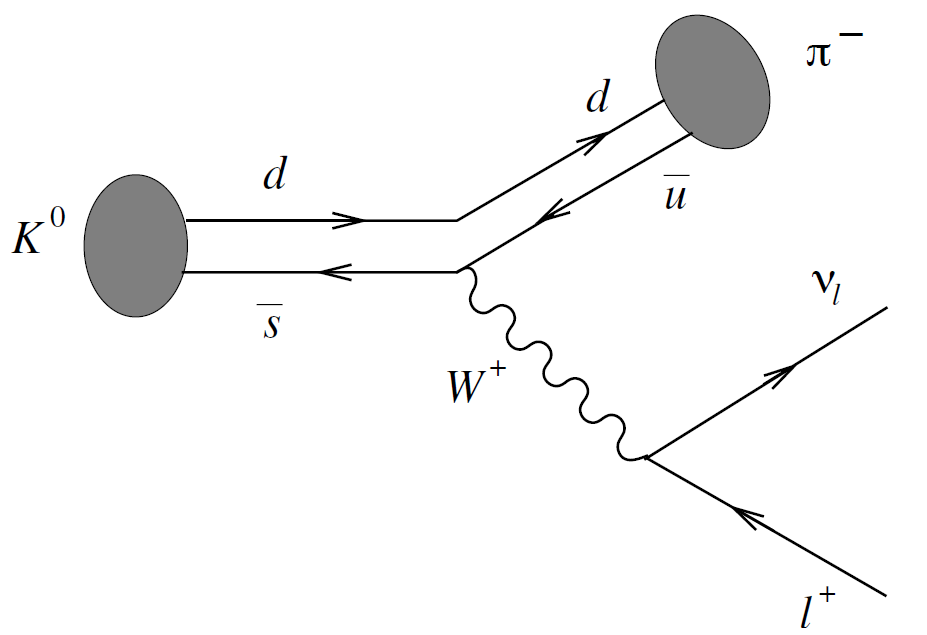
\includegraphics[width=0.4\textwidth]{figures/feyn1}
	\end{figure}
	In this case the states read $\ket{i}=\ket{\nu_l=0}\otimes \ket{l^{+}=0}\otimes\ket{K^0}$ and $\bra{f}=\bra{\pi^-}\otimes \bra{l^+}\otimes \bra{\nu_l}$. The effective Lagrangian density for the decay is given by
	\begin{equation}
		\mathcal{L}_I(0)=-\frac{G_fsin(\theta_C)}{\sqrt{2}}\bar{\nu}_l\gamma_\mu(1-\gamma^5)l\bar{s}\gamma^\mu(1-\gamma^5)u.
		\label{L2}
	\end{equation} 
	Equation \eqref{L2} is a Fermi Lagrangian density since the mediator is integrated out. It is however not an effective Lagrangian density since the coupling is specified. From equation \eqref{L2}
	\begin{equation}
		\begin{split}
			\mathcal{M}&=-\frac{G_fsin(\theta_C)}{\sqrt{2}}\bra{f}\bar{\nu}_l\gamma_\mu(1-\gamma^5)l\bar{s}\gamma^\mu(1-\gamma^5)u\ket{i}+\mathcal{O}(i^2)\\
			&=-\frac{G_fsin(\theta_C)}{\sqrt{2}}\bra{\nu_l}\bar{\nu}_l\ket{0}\gamma_\mu(1-\gamma^5)\bra{l^+}l\ket{0}\bra{\pi^-}\bar{s}\gamma^\mu(1-\gamma^5)u\ket{K^0}+\mathcal{O}(i^2)\\
			&=-\frac{G_fsin(\theta_C)}{\sqrt{2}}\bar{u}(\nu_l)\gamma_\mu(1-\gamma^5)v(l^+)\bra{\pi^-}\bar{s}\gamma^\mu(1-\gamma^5)u\ket{K^0}+\mathcal{O}(i^2),\\
		\end{split}
		\label{S12}
	\end{equation}   
	where it is understood that all matrix elements are evaluated at $x=0$. The matrix element of the quark current, i.e. the second operator, cannot be evaluated directly like the matrix element of the leptonic matrix element, i.e. the first operator. Instead the matrix element of the second operator can be parameterized in terms of form factors. The parameterization is determined by Lorentz invariance and depends in general on the specific process under consideration. The procedure to determine the amplitude in processes involving composite particles is however clear; use the Fermi Lagrangian and determine the quark-matrix elements via parameterization.
\end{example}

	
	\begin{appendices}
		\appendixpage
		\noappendicestocpagenum
		\addappheadtotoc
	
		\chapter{Code for Computational Fluid Dynamics}
\label{App:cfd}
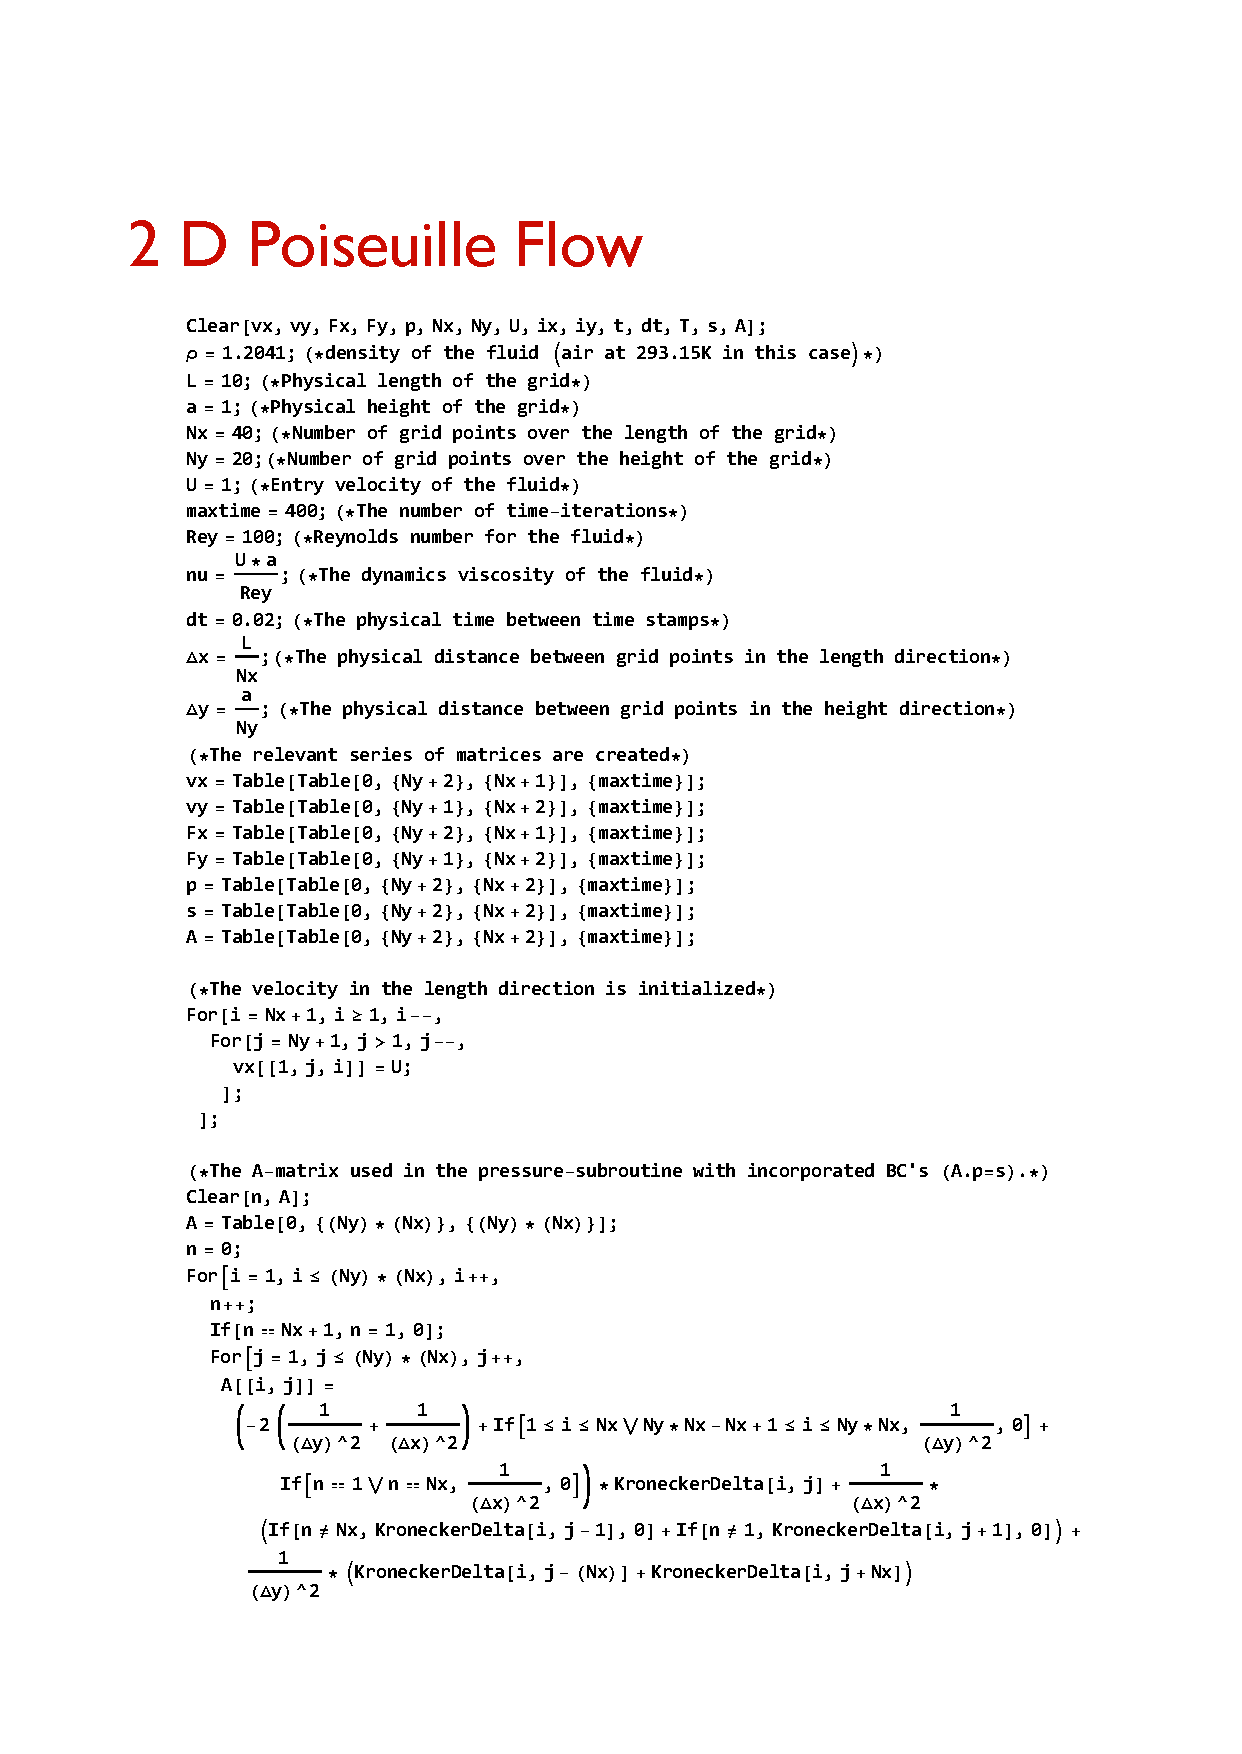
\includepdf[pages=-]{figures/2DPoiseuille.pdf}
\begin{frame}
	%	\frametitle{Forward Kinematics}	
	
	\begin{center}
		\includemedia[
		activate=onclick,
		width=0.75\textwidth
		]{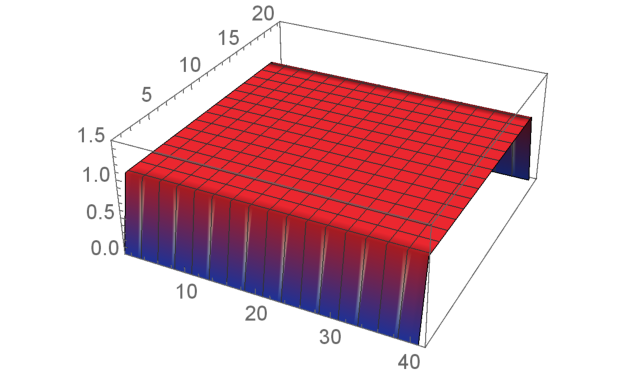
\includegraphics{figures/screensaver.pdf}}{figures/flow2.swf}
	\end{center}
\end{frame}

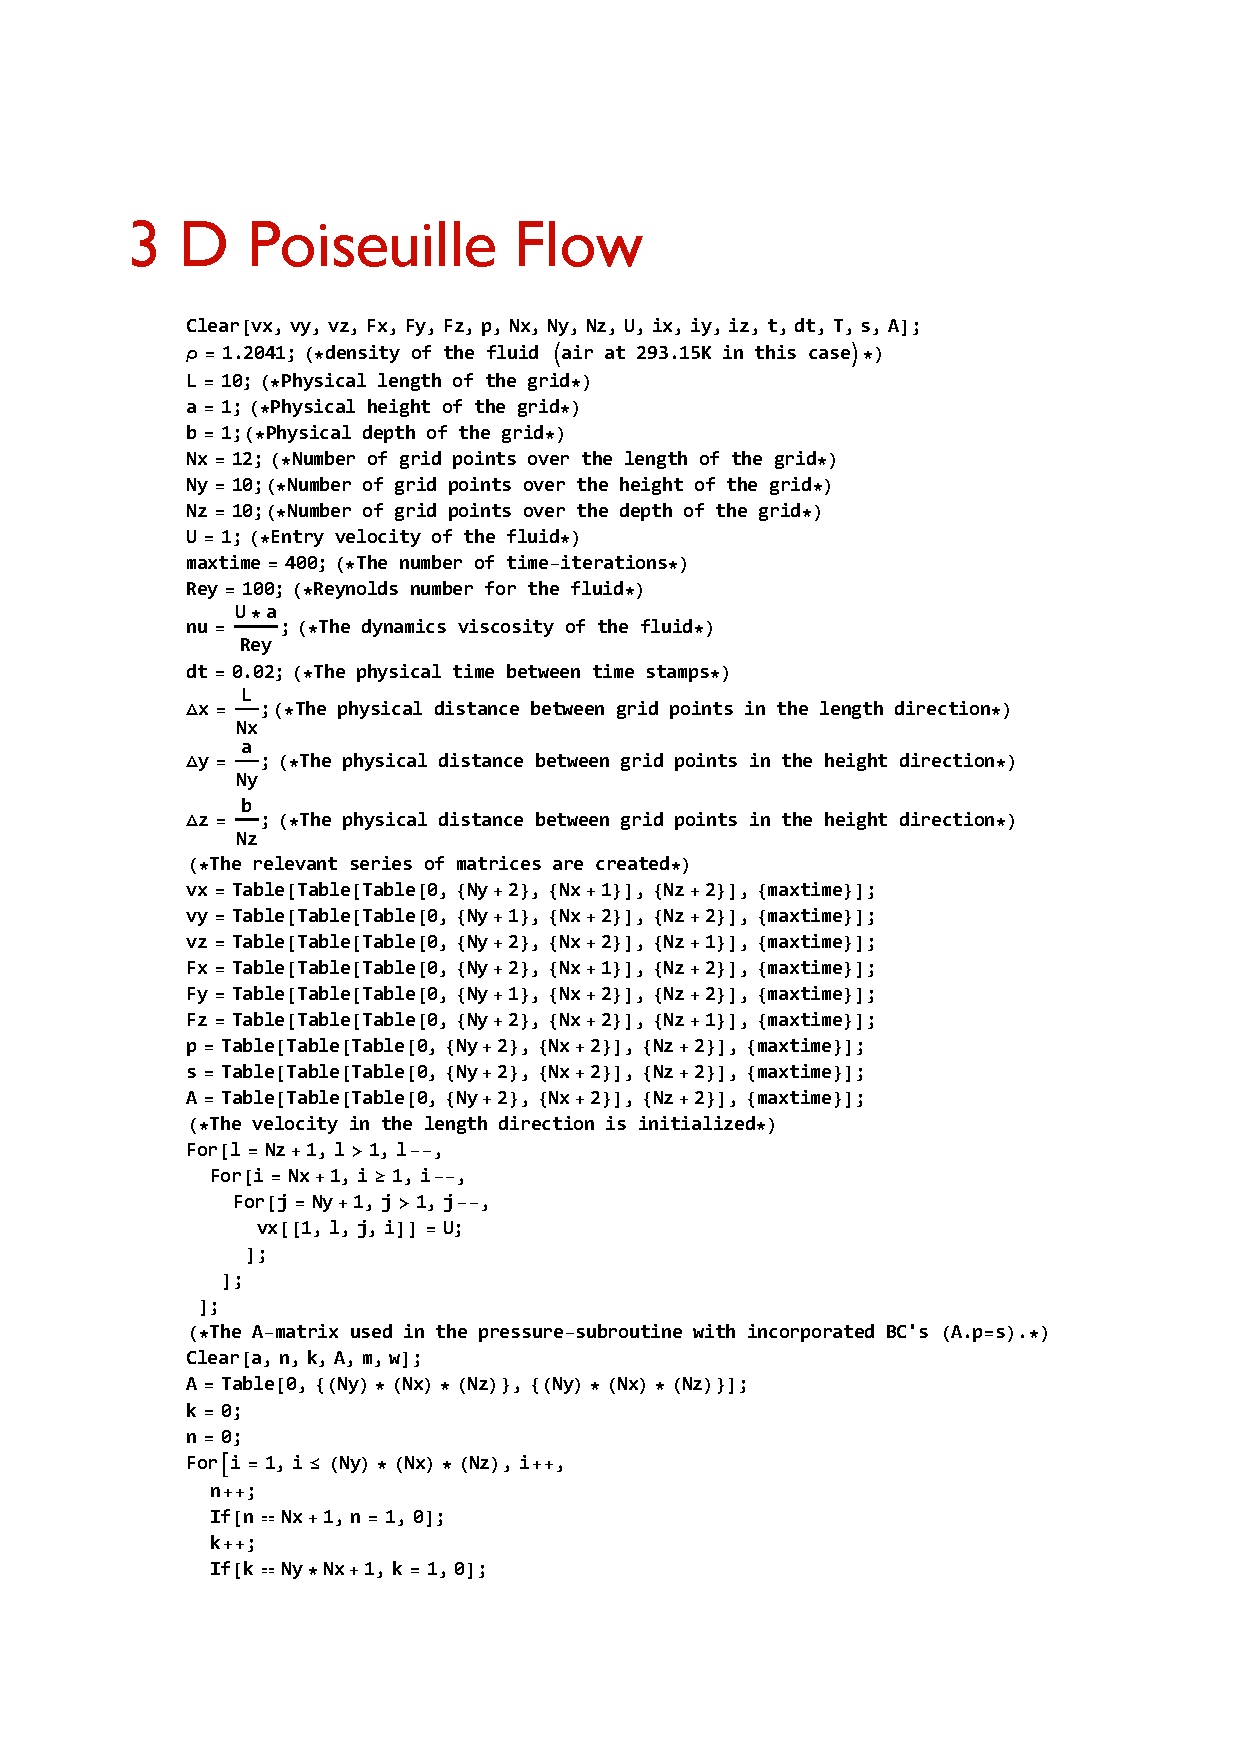
\includepdf[pages=-]{figures/3DPoiseuille.pdf}

\begin{figure}[H]
	\centering
	\captionsetup{width=1\textwidth}
	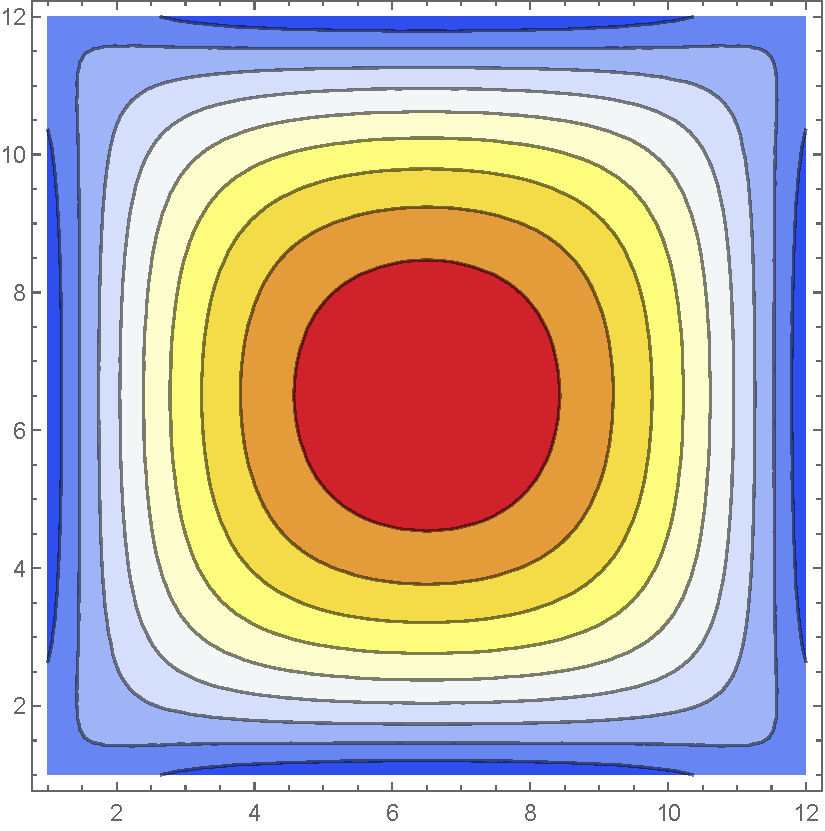
\includegraphics[width=0.3\textwidth]{figures/3D1.pdf}
	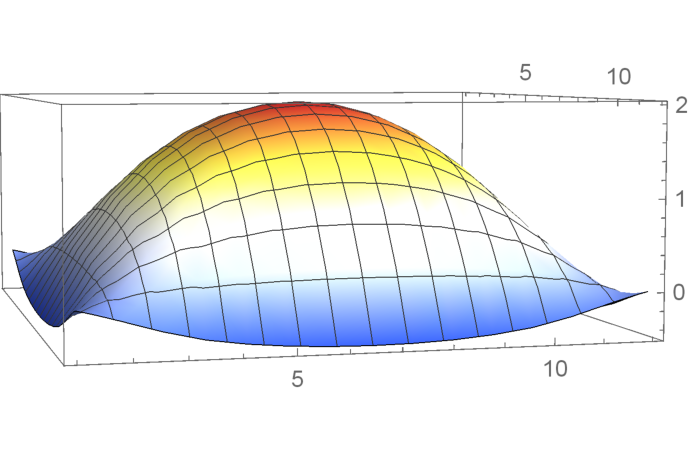
\includegraphics[width=0.3\textwidth]{figures/3D2.pdf}
	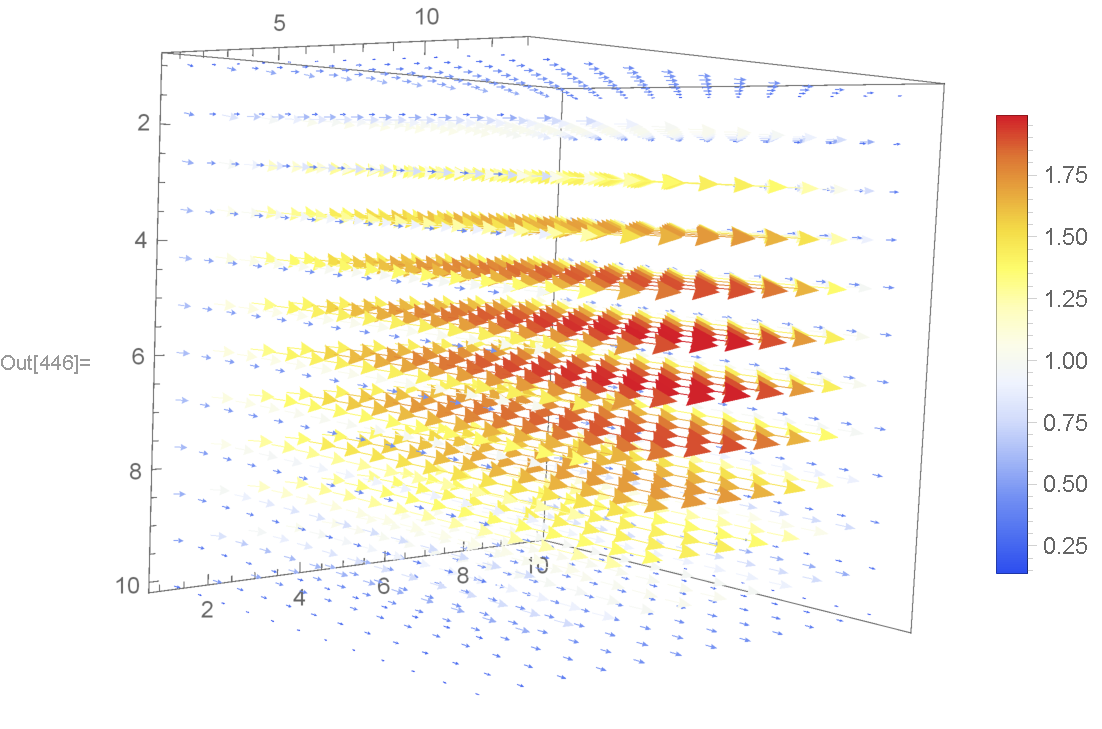
\includegraphics[width=0.3\textwidth]{figures/3D3.pdf}
	\caption
	{Left: A contour plot of the 2D slice of the flow velocity in the length direction at about halfway in the flow direction (the $x$-direction). Middle: A 3D plot of the 2D slice of the flow velocity in the length direction at the end of the channel. The height signify the value of the velocity field in the length direction. Right: A 3D vector plot of the velocity field in the channel.}
\end{figure}


\begin{frame}
	%	\frametitle{Forward Kinematics}	
	
	\begin{center}
		\includemedia[
		activate=onclick,
		width=0.75\textwidth
		]{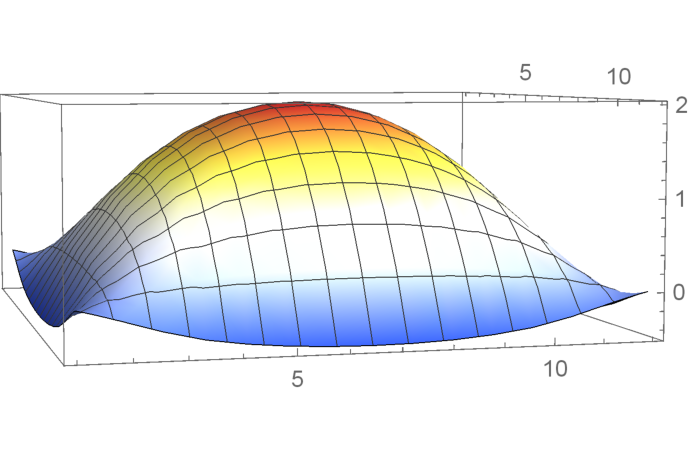
\includegraphics{figures/3D2.pdf}}{figures/flow3.swf}
	\end{center}
\end{frame}

The Navier-Stokes equations (equation \eqref{N6}) are not solve-able in the general case, and so approximations obtained from the physical scenario under consideration must be used in order to apply Navier-Stokes equations. 
		\chapter{Hamiltonian Monte Carlo}
\label{app:HMC}
This appendix is taken from \citet{petersen2020}. The Hamiltonian Monte Carlo Algorithm (HMC algorithm) is a Markov Chain Monte Carlo (MCMC) algorithm used to evaluate integrals on the form
\begin{equation}
	\begin{split}
		\mathbb{E}[f] &= \int f(\theta)g(\theta)d\theta\\
		& \approx \frac{1}{N}\sum_{j\in g}f(\theta_j),
	\end{split}
\end{equation}
with $f$ being a generic function and $N$ denoting the number of samples from the posterior distribution, $g$. The sample $\{j\}$ from $g$ can be generated via a MCMC algorithm that has $g$ as a stationary distribution. The Markov chain is defined by an initial distribution for the initial state of the chain, $\theta$, and a set of transition probabilities, $p(\theta'|\theta)$, determining the sequential evolution of the chain. A distribution of points in the Markov Chain are said to comprise a stationary distribution if they are drawn from the same distribution and that this distribution persist once established. Hence, if $g$ is the a stationary distribution of the Markov Chain defined by the initial point $\theta$ and the transition probability $p(\theta'|\theta)$, then~\citep{Neal:1996}
\begin{equation}
	g(\theta')=\int p(\theta'|\theta)g(\theta)d\theta.
	\label{ee1}
\end{equation}
Equation \eqref{ee1} is implied by the stronger condition of detailed balance, defined viz
\begin{equation}
	p(\theta'|\theta)g(\theta)=p(\theta|\theta')g(\theta').
\end{equation}
A Markov chain is ergodic if it has a unique stationary distribution, called the equilibrium distribution, to which it converge from any initial state. $\{i\}$ can be taken as a sequential subset (discarding the part of the chain before the equilibrium distribution) of a Markov chain that has $g(\theta)$ as its equilibrium distribution. \newline
The simplest MCMC algorithm is perhaps the Metropolis-Hastings (MH) algorithm ~\citep{Metropolis1953,hastings70}. The MH algorithm works by randomly initiating all coefficients for the distribution wanting to be sampled. Then, a loop runs a subjective number of times in which one coefficient at a time is perturbed by a symmetric proposal distribution. A common choice of proposal distribution is the normal distribution with the coefficient value as the mean and a subjectively chosen variance. If $g(\theta')\geq g(\theta)$ the perturbation of the coefficient is accepted, otherwise the perturbation is accepted with probability $\frac{g(\theta')}{g(\theta)}$.\newline
The greatest weaknesses of the MH algorithm is i) a slow approach to the equilibrium distribution, ii) relatively high correlation between samples from the equilibrium distribution and iii) a relatively high rejection rate of states. ii) can be rectified by only accepting every $n$'th accepted state, with $n$ being some subjective number. For $n\rightarrow \infty$ the correlation naturally disappears, so there is a trade off between efficiency and correlation. Hence, in the end the weaknesses of the MH algorithm can be boiled down to inefficiency. This weakness is remedied by the HCM algorithm~\citep{Duane:1987de} in which Hamiltonian dynamics are used to generate proposed states in the Markov chain and thus guide the journey in parameter space. Hamiltonian dynamics are useful for proposing states because~\citep{Neal2012} 1) the dynamics are reversible, implying that detailed balance is fulfilled and so there exist a stationary distribution, 2) the Hamiltonian ($H$) is conserved during the dynamics if there is no explicit time dependence in the Hamiltonian ($\frac{dH}{dt}=\frac{\partial H}{\partial t}$), resulting in all proposed states being accepted in the case the dynamics are exact and 3) Hamiltonian dynamics preserve the volume in phase space ($q_i,p_i$-space), which means that the Jacobian is unity (relevant for Metropolis updates that succeeds the Hamiltonian dynamics in the algorithm). By making sure the algorithm travel (in parameter space) a longer distance between proposed states, the proposed states can be ensured to have very low correlation, hence alleviating issues 1) and 2) of the MH algorithm. The price to pay for using the HMC algorithm relative to the MH algorithm is a) the HMC algorithm is gradient based meaning it requires the Hamiltonian to be continuous and b) the computation time can be long depending on the distribution being sampled (e.g. some recurrent ANNs are computationally heavy due to extensive gradient calculations).\newline
As previously stated, the HMC algorithm works by drawing a physical analogy and using Hamiltonian dynamics to generate proposed states and thus guide the journey in parameter space. The analogy consists in viewing $g$ as the canonical probability distribution describing the probability of a given configuration of parameters. In doing so, $g$ is related to the Hamiltonian, $H$, viz
\begin{equation}
	g=e^{\frac{F-H}{k_BT}}\Rightarrow H=F-k_BT\ln[g],
\end{equation}
where $F=-k_BTln[Z]$ denotes Helmholtz free energy of the (fictitious in this case) physical system and $Z$ is the partition function. $\ln[g(\theta)]$ contain the position (by analogy) variables of the Hamiltonian and so $Z$ must contain the momentum variables. Almost exclusively~\citep{Betancourt2013} $Z\sim \mathcal{N}(0,\sqrt{m_i})$ is taken yielding the Hamiltonian 
\begin{equation}
	H=-k_BT\bigg[\ln[g]-\sum_{i}\frac{p_i^2}{2m_i}\bigg]+const,
\end{equation}
where $i$ run over the number of variables and "const" is an additive constant (up to which the Hamiltonian is always defined). $T=k_b^{-1}$ is most often taken~\citep{Neal2012}, however, the temperature can be used to manipulate the range of states which can be accepted e.g. via simulated annealing~\citep{MacKay2002}. Here $T=k_b^{-1}$ will be adopted in accordance with \citep{Neal:1996,Neal2012} and as such
\begin{equation}
	H=\sum_{i}\frac{p_i^2}{2m_i}-\ln[g].
\end{equation}
The dynamics in parameter space are determined by Hamiltons equations
\begin{equation}
	\dot{\theta}_i=\frac{\partial H}{\partial p_i},\qquad \dot{p}_i=-\frac{\partial H}{\partial \theta_i},
\end{equation}
with $\theta_i$ denoting the different variables (coefficients). In order to implement Hamiltons equations, they are discretized via the leap frog method~\citep{Neal:1996,Neal2012} viz
\begin{equation}
	\begin{split}
		&p_i\left( t+\frac{\epsilon}{2}\right)=p_i(t)-\frac{\epsilon}{2}\frac{\partial H(\theta_i(t),p_i(t))}{\partial \theta_i},\\
		&\theta_i(t+\epsilon)=\theta_i(t)+\frac{\epsilon}{m_i}p_i\left(t+\frac{\epsilon}{2}\right),\\
		&p_i(t+\epsilon)=p_i\left(t+\frac{\epsilon}{2}\right)-\frac{\epsilon}{2}\frac{\partial H(\theta_i(t+\frac{\epsilon}{2}),p_i(t+\frac{\epsilon}{2}))}{\partial \theta_i},\\
	\end{split}
\end{equation}
with $\epsilon$ being an infinitesimal parameter. In the algorithm the initial state is defined by a random initialization of coordinates and momenta, yielding $H_{initial}$. Subsequently Hamiltonian dynamics are simulated a subjective ($L$ loops) amount of time resulting in a final state, $H_{final}$, the coordinates of which take the role of proposal state. The loop that performs $L$ steps of $\epsilon$ in time is here referred to as the dive. During the dive, the Hamiltonian remains constant, so ideally $H_{initial}=H_{final}$, however, imperfections in the discretization procedure of the dynamics can result in deviations from this equality (for larger values of $\epsilon$, as will be discussed further later on). For this reason, the proposed state is accepted as the next state in the Markov chain with probability
\begin{equation}
	\mathbb{P}(\rm transition)=\min\big[1,e^{H_{initial}-H_{final}}\big].
	\label{pro}
\end{equation}
Whether or not the proposed state is accepted, a new proposed state is next generated via Hamiltonian dynamics and so the loop goes on for a subjective amount of time. \newline
Most often, the HMC algorithm will be ergodic, meaning it will converge to its unique stationary distribution from any given initialization (i.e. the algorithm will not be trapped in some subspace of parameter space), however, this may not be so for a periodic Hamiltonian if $L\epsilon$ equal the periodicity. This potential problem can however be avoided by randomly choosing $L$ and $\epsilon$ from small intervals for each iteration. The intervals are in the end subjective, however, with some constraints and rules of thumb; the leap frog method has an error of $\mathcal{O}(\epsilon^2)$~\citep{Neal:1996} and so the error can be controlled by ensuring that $\epsilon\ll1$. A too small value of $\epsilon$ will waste computation time as a correspondingly larger number of iterations in the dive ($L$) must be used to obtain a large enough trajectory length $L\epsilon$. If the trajectory length is too short the parameter space will be slowly explored by a random walk instead of the otherwise approximately independent sampling (the advantage of non-random walks in HMC is a more uncorrelated Markov chain and better sampling of the parameter space). A rule of thumb for the choice of $\epsilon$ can be derived from a one dimensional Gaussian Hamiltonian
\begin{equation}
	H=\frac{q^2}{2\sigma^2}+\frac{p^2}{2}.
	\label{ghf}
\end{equation}
The leap frog step for this system is a linear map from $t\rightarrow t+\epsilon$. The mapping can be written
\begin{equation}
	\begin{split}
		\begin{bmatrix}
			q(t+\epsilon)\\
			p(t+\epsilon)
		\end{bmatrix}&=\begin{bmatrix}
			1-\frac{\epsilon^2}{2\sigma^2}& \epsilon\\
			\epsilon(\frac{1}{4}\epsilon^2\sigma^{-4}-\sigma^{-2}) & 1-\frac{1}{2}\epsilon^2\sigma^{-2}\\
		\end{bmatrix}\begin{bmatrix}
			q(t)\\
			p(t)
		\end{bmatrix}\\
	\end{split}
\end{equation}
The eigenvalues of the coefficient matrix represent the powers of the exponentials that are the solutions to the differential equation. They are given by
\begin{equation}
	\text{Eigenvalues}=1-\frac{1}{2}\epsilon^2\sigma^{-2}\pm \epsilon\sigma^{-1}\sqrt{\frac{1}{4}\epsilon^2\sigma^{-2}-1}.
\end{equation}
In order for the solutions to be bounded, the eigenvalues must be imaginary, meaning that
\begin{equation}
	\epsilon<2 \sigma.
	\label{gh}
\end{equation}
In higher dimensions a rule of thumb is to take $\epsilon\lesssim 2\sigma_x$, where $\sigma_x$ is the standard deviation in the most constrained direction, i.e. the square root of the smallest eigenvalue of the covariance matrix. In general~\citep{Betancourt2013} a stable solution with $\frac{1}{2}p^T\Sigma^{-1}p$ as the kinetic term in the Hamiltonian require 
\begin{equation}
	\epsilon_i<2 \lambda_i^{-\frac{1}{2}},
	\label{laa}
\end{equation}
for each eigenvalue $\lambda_i$ of the matrix
\begin{equation}
	M_{ij}=(\Sigma^{-1})_{ij}\frac{\partial^2 H}{\partial q_i\partial q_j},
\end{equation}
which means that in the case of $\Sigma^{-1}=diag(m_i^{-1})$;
\begin{equation}
	\epsilon_i<2\sqrt{\frac{m_i}{\frac{\partial^2H}{\partial q^2_i}}}.
	\label{heu}
\end{equation}
Setting $\epsilon$ according to equation \eqref{laa} can however introduce issues for hierarchical models (models including hyper parameters) since the reversibility property of Hamiltonian dynamics is broken if $\epsilon$ depend on any parameters. This issue can be alleviated by using the MH algorithm on a subgroup of parameters~\citep{Neal:1996,Neal2012} (which are then allowed in the expression for $\epsilon$) that is to be included in $\epsilon$. However, unless the MH algorithm is used for all parameters, some degree of approximation is required. The HMC algorithm is shown in algorithm \ref{alg:HMC}.
\vspace{5mm} %5mm vertical space

\begin{algorithm}
	\label{alg:HMC}
	\caption{Hamiltonian Monte Carlo Algorithm in pseudo code}
	\textbf{Save:} $q$ and $V(q)$, with $q$ randomly initialized\;
	\For{i<N+1}{
		$p =$ Sampled from standard normal distribution\;
		$H_{old} = H(q, p)$\;
		$p = p - \frac{\epsilon}{2}\frac{\partial H(q,p)}{\partial q}$\;
		$L=RandomInteger(L_{lower}, L_{upper})$\;
		\For{j<L+1}{
			$q = q + \epsilon \frac{p}{mass}$\;
			\If{$j\neq L$}{
				$p = p - \epsilon\frac{\partial H(q,p)}{\partial q}$\;
			}
		}
		$p = p - \frac{\epsilon}{2}\frac{\partial H(q,p)}{\partial q}$\;
		$H_{new}=H(q,p)$\;
		$u=$ Sample from uniform distribution\;
		\If{$u<\min(1, e^{-(H_{new}-H_{old})})$}{
			$H_{old}=H_{new}$\;
			{\bf Save:} $q$ and $V(q)$\;
		}
		
	}
\end{algorithm}
\vspace{5mm} %5mm vertical space
		\include{app_nested_sampling}
	
	\end{appendices}
	
	
	\bibliographystyle{plainnat}
	\bibliography{refs}
	
	\clearpage
	\printindex{}

\end{document}